\documentclass[a4paper, 11pt, english]{book} %, openright
% \usepackage[doublespacing]{setspace}
%mettere oneside dopo la lingua per stampare solo fronte
% \usepackage[toc,page]{appendix}
% \usepackage{array, afterpage, 
\usepackage{amsfonts, amsmath, amsthm, amssymb, accents}
% \usepackage{babel}
% \usepackage{bbm, bm, booktabs}
% \usepackage{caption}
% \usepackage{capt-of}
% \usepackage{chngcntr}
% \usepackage{commath}
\usepackage{booktabs}
\usepackage[sectionbib]{chapterbib}
\usepackage{cancel}
% \usepackage{datetime}
% \usepackage{epstopdf, enumitem}
% \usepackage{etoolbox}
% \usepackage{fancyvrb, floatrow}
\usepackage{notomath}
\usepackage[T1]{fontenc}
\usepackage[inner=2.5cm,outer=2.5cm,bottom=4cm,top=3cm]{geometry}
\usepackage{graphicx}
\usepackage{hyperref}
\usepackage[utf8]{inputenc}
% \usepackage{lipsum}
% \usepackage{lscape}
% \usepackage{lmodern, longtable}
% \usepackage{marginnote, mathrsfs}
% \usepackage{multirow}
\usepackage[square,numbers]{natbib}
\bibliographystyle{apalike}
\usepackage{pifont}
\newcommand{\cmark}{\ding{51}}
\newcommand{\xmark}{\ding{55}}
% \usepackage{rotating}
\usepackage{soul}
% \usepackage{subfigure}
% \usepackage{stmaryrd}
% \usepackage{titlesec}
\usepackage{tikz}
\tikzset{
	position label/.style={
		below = 3pt,
		text height = 1.5ex,
		text depth = 1ex
	},
	brace/.style={
		decoration={brace, mirror},
		decorate
	}
}
\usetikzlibrary{arrows,positioning,patterns,decorations.pathreplacing} 
\usepackage{url}
\usepackage{wrapfig}

\newcounter{appendix}[chapter]
\linespread{1.2} %interlinea 

\newtheorem{definition}{Definition}
\newtheorem{theorem}{Theorem}
\newtheorem{proposition}{Proposition}
\newtheorem{corollary}{Corollary}
\newtheorem{lem}{Lemma}
\newtheorem{example}{Example}
\newtheorem{remark}{Remark}
\newtheorem{defi}{Definition}[section]
\newtheorem{prop}{Proposition}[section]

% \author{}

%\input{Preamble}
\newcommand{\EE}{\mathbb{E}}
\newcommand{\dd}{\mathrm{d}}
\newcommand{\dbtilde}[1]{\accentset{\approx}{#1}}

\newenvironment{abstract}{%
\clearpage\thispagestyle{empty}\vspace*{3\baselineskip}
\begin{center}\textbf\abstractname\end{center}
\begin{quotation}
}{\end{quotation}\clearpage}

\begin{document}
%	\hypersetup{pageanchor=false}
%	\thispagestyle{empty}
%	\fontsize{3.76mm}{5mm}\selectfont
%	\input{Declaration}
%	\hypersetup{pageanchor=true}
\begin{titlepage}
	\Large
	\begin{center}
		{\LARGE \textsc{Università Commerciale ``Luigi Bocconi''} } \\
		{\LARGE \textsc{PhD School} }
		\vspace{1.5cm} \\
		\begin{raggedright}
			PhD program in: Statistics \\
			Cycle: XXXV \\
			Disciplinary Field (code): SECS-S/01\\
		\end{raggedright}
		\vfill
		
		{\Huge \bfseries Risk prediction and family history effect in survival models for disease onset, with a specific focus on breast cancer}
		\vfill
		
		\begin{raggedright}
			Advisor: Marco Bonetti \\
			%Co-Advisor (if any): \texttt{[coa\_name] [coa\_surname]} \\
		\end{raggedright}
		
		\vspace{1.5cm}
		
		\begin{raggedleft}
			PhD Thesis by \\
			Maria Veronica Vinattieri \\
			ID number: 3111885 \\
		\end{raggedleft}
		
		\vfill
		
		\textbf{Year: 2024}
	\end{center}
\end{titlepage}

\thispagestyle{empty}
%\fontsize{3.76mm}{5mm}\selectfont
\chapter*{Acknowledgements}
I would like to thank my supervisor Marco Bonetti for pushing me to always do my best, for his enthusiasm and meticulous attention to detail. 

I would like to thank Kamila Czene and Keith Humphreys for their precious advises, for inviting and hosting me in Karolinska Instituetet with the support of grant 2022-00584 with PI Kamila Czene. 

I would like also to thank the population dynamics and health unit of the Carlo F. Dondena research center at Bocconi University for its support. 

I would like to thank all the colleagues that I have met during the PhD in Bocconi, you have been my Milanese family. Especially, I would like to thank my colleagues from my year, it has been a pleasure to share this journey with you and I have learned so much from you. 

I would like to thank all my loved ones, I won't give names but you know exaclty who you are and how much I am grateful for your support, for listening to me and offering advice when things get tough, for making me laugh and always making me feel right at home. 
\chapter*{Abstract}
We are interested in a specific aspect related to modeling disease development, i.e. the study of family-specific risk. Generally, quantifying the family-specific risk of developing a disease is crucial to improve the patient’s survival, and healthcare data provide an essential tool to estimate such quantity. Specifically for breast cancer, early detection is particularly important to increase the chances of a successful treatment. In this setting, risk estimation allows for the identification of subjects at higher risk of developing breast cancer, so that they can be the target of tailored
and more intensive screening and prevention strategies. We take families as our statistical units of interest, and we assume that these units belong to different risk groups of developing the disease. We investigate models on the age at breast cancer onset, with a structure of familiar dependence among survival times through the risk.
In Chapter 1, we compare cure rate models with a continuous Gamma frailty to the conventional Cox model in terms of risk prediction accuracy. In Chapter 2, however, we focus exclusively on cure rate models using a binary frailty to model the age at onset. In Chapter 3 we move to the study of the heritability of longevity. Similarly to the previous chapters, we assume that families have different “risk” in terms of life expectancy. We carry out our analysis through simulation studies and apply the continuous frailty model from Chapter 1 to the available data sourced from the Multi-Generational Breast Cancer Swedish registry. We conclude with the exploration of most powerful tests on survival data with right censoring in Chapter 4.
\chapter*{Introduction}
We focus on a specific aspect of modeling the disease development, namely the investigation of family-specific risk. Generally, quantifying the family-specific risk of developing a disease is crucial to improve early detection of the disease and consequently the patient’s survival. Healthcare data provide an essential tool to estimate the family-specific risk, and thus we develop and employ specific methods to estimate this risk from the available data. We focus on breast cancer onset,  although the problem can be generalized to a wide range of diseases. In the context of breast cancer development, risk estimation plays a crucial role in identifying families, and thus individuals, who are at the highest risk of developing breast cancer. We assume that individuals who belong to the same family share a common risk of being diagnosed with breast cancer from birth. Thus, this family-specific risk is unchanged from birth and never observable. Because of the latent nature of the risk we call it the frailty risk. Once we identify the highest-risk families, that are those with highest values of the frailty risk, we can target family´s female members for tailored and more intensive screening and prevention strategies, which can improve their chances of a successful treatment and prognosis.

One common approach to split families into different risk groups of developing breast cancer is considering the strongest risk factors associated to breast cancer development. In our motivating data, one among the strongest risk factors is available: the breast cancer family history.  The breast cancer family history is defined as the indicator of observing at least one family member who has already experienced breast cancer diagnosis at a fixed time. Specifically, the family history indicator $FH(t)$ takes value one when, at time $t$, at least one family member has been diagnosed with invasive breast cancer, otherwise it takes value $0$. This indicator is based on the notion that individuals with a positive (i.e. $FH(t) = 1$) family history are at a higher risk of developing breast cancer itself. From one side it is convenient to involve this easy indicator into a model with the aim of splitting families into groups, that are in total two: the low-risk group and the high-risk group of developing breast cancer. Also, this approach motivates the categorization of families into two frailty risk groups, allowing the frailty risk to be binary with two levels $0/1$, for low and high-risk groups respectively, as we illustrate in Chapter \ref{chapter:2}. On the other side the family history, and consequently the binary frailty risk, cannot capture the complex nature of such a phenomenon as breast cancer development. This motivates our primary novel contribution of this thesis that is the extension of the frailty risk to be continuous with infinitely many values, as we illustrate in Chapter \ref{chapter:1}.  Specifically, the continuous frailty risk is assumed to be distributed according to a Gamma distribution with parameters $(shape=\theta, \ rate=\theta)$, where we call $\theta$ the frailty parameter. Once we assume a continuous frailty risk we carry out a comparative analysis to assess that our proposed model, namely the Multivariate frailty Cure-Rate model, outperforms among the other models under analysis in terms of inference precision, prediction accuracy, and explanability of the phenomenon. The multivariate part of our proposed model refers to jointly model the family female members time-to-events (where the event of interest is breast cancer onset in our case) in contrast to modelling only one subject per family, as the Univariate frailty Cure-Rate model or the Univariate FH Cure-Rate model do, as we develop and see in Chapter \ref{chapter:1}.  While, the Cure-Rate component refers to the peculiar structure that the survival function takes based on the assumption that not all the women will experience breast cancer onset eventually in their lifetime. The proportion of women that won´t experience the breast cancer onset is called the cured fraction. The cured fraction enters then the Cure-Rate survival function formula, making the survival function not proper anymore as we will see deeper into Chapter \ref{chapter:1}. Thus, through the Multivariate frailty Cure-Rate model our novel contribution consists of involving the Cure-Rate baseline survival function in a Lehmann structure that unites the different family-specific frailty risk survival functions. In other words, each family has a specific survival function that depends on the Cure-Rate baseline survival function and on its frailty risk values through the Lehmann structure. Moreover, we prove that also the family-specific frailty survival function follows a Cure-Rate structure itself.  

Hence, the Multivariate frailty Cure-Rate model allows us to estimate the survival distribution of  ``cases'', that are defined as those women that will eventually experience the breast cancer onset in their lifetime, and to capture a peculiar tail behaviour by estimating the cured fraction. These measures accurately contribute to explain the magnitude of breast cancer development into the population of interest. In contrast, for example, a more flexible model as the already known and developed Multivariate frailty Cox model would not allow us to estimate such quantities. Moreover, we show that Multivariate frailty Cure-Rate model achieves a level of prediction accuracy on par to the Multivariate frailty Cox model. This highlights the superior potential of our proposed model over the traditional Cox model, leaving no room for uncertainty that the Multivariate frailty Cure-Rate model strikes a balance among precision in inference and explainability of the phenomenon without losing points about prediction accuracy. 

% Our main assumption is that , and we must employ appropriate methods to deal with the problem of missing information due its latency. 

% To achieve this goal, we take families as our units of interest and assume that they have a value of the frailty risk among the infinitely many in Chapter \ref{chapter:1}. While in Chapter \ref{chapter:2} we assume that families can be categorized into two latent risk groups based on their risk of developing the disease, thus the risk $R$ is allowed to be binary with two levels $0/1$, for low and high-risk groups respectively.

% The main raw purpose here is to estimate the frailty parameter, that is necessary for computing the posterior family-specific risk of breast cancer occurrence. The estimation of the frailty parameter can occur through several implemented models. We explore a total of six models, with three of them that are semiparametric, and three of them that are parametric. Specifically, we implement a model that we call ``multivariate'', meaning that the complete family information from all the family members on breast cancer history is jointly model to accurately estimate the frailty. Two multivariate model are implemented: our frailty parametric model and the semiparametric Cox model. The other models are called ``univariate'' to indicate that only one subject per family is involved. One of the them is a univariate frailty model, while the other tree replace the unknown frailty quantity with a summary of the family history (FH) of breast cancer as a covariate.

% With the estimate of the frailty parameter we can estimate the poster family-specific risk distribution, and thus the risk can be estimated as the posterior mean, median, or mode. For ease of interpretation and better performances in prediction accuracy, we select the mean as frailty estimate. 

% From the analysis, we expect that the multivariate models perform better in terms of risk prediction accuracy compared to the other models, since they are jointly modelling all the familiar information. Moreover, we expect that the parametric multivariate model performs better than its semiparametric counterpart in terms of precision in inference, prediction accuracy, and interpretability of the phenomenon.

% Notably, let us say that all the parametric models that we implement follow a cure rate survival structure which assume that not all women will develop breast cancer in their lifetime, in contrast to the traditional survival model which assumes that all individuals will experience the event eventually. We believe that the cure rate structure is more realistic as a representation of breast cancer development, as it allows for the possibility of some individuals not to develop the disease. This is an additional reason why we believe the parametric multivariate model to be better then its semiparametric counterpart because it can estimate the cured fraction that accurately contributes to explain the magnitude of the phenomenon of worldwide interest that is the breast cancer development.

% After preliminary simulation studies, a real analysis has been carried out on an outstanding dataset, based on the Multi-generational Swedish Breast Cancer registry, that Kamila Czene from the Medical Epidemiology and Biostatistics (MEB) department of Karolinska Institutet in Stockholm, Sweden provided to us. 

Similarly we obtain in Chapter \ref{chapter:2} where, as already mentioned above, the family history approach motivates the use of a binary frailty risk to split families into two risk groups. Indeed here, the comparison between the Multivariate frailty Cure-Rate model and the Univariate frailty Cure-Rate to the Univariate FH Cure-Rate model is more meaningful than in the previous chapter thanks to the same binary nature of the frailty risk and the risk factor used as its replacement. Nevertheless, the Univariate FH Cure-Rate model may be not accurate in explaining the breast cancer development. And so may be the Univariate frailty Cure-Rate model. From results, the Multivariate frailty Cure-Rate model outperforms the other two models in terms of accuracy in risk prediction. 

Modelling a continuous frailty risk allows us to capture the complexity of the phenomenon of the breast cancer development and deal with this problem in a real dataset, beyond simulation studies. On the other side, modelling a binary frailty risk might seem simpler and more direct, but with the drawback of not capturing the real differences in risk among families, moreover in a large dataset as we have. Let us say that splitting families into two categories and identifying the higher-risk families remains clinically convenient. That is why we have included a section in Chapter  \ref{chapter:1} discussing the transition from infinitely many values of the risk among families to only two values of the risk (low and high) by splitting the families according to a fixed threshold. 

One strength of this thesis is the use of the Cure-Rate survival function in contrast to the traditional survival function that tends to 0 when the time-to-event tends to $+\infty$, meaning that all individuals will experience the event of interest eventually. For sake of completeness, we want to study also the use of a traditional survival function on the event death, as we firmly believe that with another event such as disease onset we should use a Cure-Rate survival function. On the other side, not to be too far from the study of the family-specific frailty risk of developing breast cancer, we move to the study of family-specific frailty risk of mortality in Chapter \ref{chapter:3} or, in more optimistic words, the heritability of longevity within families. Indeed, we believe that families belong to different groups of life expectancy according to their common genetics (internal factors) and life-habits (external factors). Similarly to the other two chapters, the focus in on posterior risk prediction through summarizing the posterior risk distribution. The novel contribution here is the development of a classification algorithm that operates to compute the posterior distribution of the risk of mortality. The algorithm implemented is applied to scenarios involving both discrete k-level risk or continuous risk. Additionally, we explore the binary splitting as an alternative approach to identify families into two risk groups, where one has higher life expectancy than the other. This also resembles the framework of Chapter \ref{chapter:1} and Chapter \ref{chapter:2}. Hence, it is of interest how, beyond contributing to the explanation of heritability of longevity, there is the chance to link mortality to disease onset by addressing families with the lowest life expectancy to strategies of clinical prevention of diseases and also improvement of their life habit routine.  

One notable aspect of this thesis lies in its expansion of the Lehmann family to the Cure-Rate models. While our primary focus has been on Cure-Rate models thus far, the concluding and most theoretically rich chapter in this thesis delves into the application of the Lehmann structure to proportional hazards models. Here, we delve into the traditional survival functions, and the prospect of extending our work to include Cure-Rate models emerges as a direct and intriguing extension. Thus, the exploration of most powerful tests for survival data with and without right censoring has been carried out in Chapter \ref{chapter:4}. Under the proportional hazards assumption we aim to evaluate whether an independently and identically distributed (i.i.d.) sample from a population exhibits survival times that are governed by a known survival function denoted as $S_0(t)$, rather than being governed by an unknown survival function denoted by $S_1(t)=[S_0(t)]^{\beta}$, with $\beta$ not equal to one. 

To better understand aims, findings and connections between the chapters of the thesis I proposed two tables (Tables \ref{table:1}, and \ref{table:2}) which briefly summarize all the work done.

\textcolor{blue}{\begin{center}
\begin{table*}[!h]%
\caption{Connection among the chapters.}
\begin{tabular*}{\textwidth}{@{\extracolsep\fill}lllll@{}}
    \toprule
    &Lehmann &Survival function &Event of interest &Frailty risk \\ \midrule 
    Chapter 1 &\cmark &Cure-Rate &Breast Cancer onset &Continuous \\
    Chapter 2 &\cmark &Cure-Rate &Breast Cancer onset &Binary \\
    Chapter 3 &\cmark &Traditional &Death &Discrete/Continuous \\
    Chapter 4 &\cmark &Traditional &Disease onset &\xmark \\ \bottomrule
    \end{tabular*}
\label{table:1}
\end{table*}
\end{center} }

\begin{center}
\begin{table*}[!h]%
\caption{Aims and findings.}
\begin{tabular*}{\textwidth}{@{\extracolsep\fill}ll@{}}
    \toprule
    &Aims and findings \\ \midrule 
    Chapter 1 &The Multivariate frailty Cure-Rate model outperforms the others. \\
    Chapter 2 &The Multivariate frailty Cure-Rate model outperforms the others. \\
    Chapter 3 &An algorithm for risk prediction has been developed. \\
    Chapter 4 &An application of the Lehmann family to PH models has been developed. \\ \bottomrule
    \end{tabular*}
\label{table:2}
\end{table*}
\end{center} 



% \include{Abstract/Abstract}
% \clearpage\setcounter{page}{1}
\tableofcontents %indice
\markboth{\textsc{Contents}}{\textsc{Contents}}

\chapter{An Application of risk prediction models to the Swedish Multi-Generational Breast Cancer Registry}{Joint work with Kamila Czene.\footnote{Department of Medical Epidemiology and Biostatistics, Karolinska Institutet, Solna, 171 77, Sweden, email: kamila.czene@ki.se.} In progress.}
\markboth{\textsc{Risk prediction models for breast cancer}}{\textsc{Risk prediction models for breast cancer}}\label{chapter:1}
% \author[1]{\fnm{Maria Veronica} \sur{Vinattieri}}\email{maria.vinattieri@phd.unibocconi.it}

% \author[2]{\fnm{Marco} \sur{Bonetti}}\email{marco.bonetti@unibocconi.it}
% % \equalcont{These authors contributed equally to this work.}

% \author[3]{\fnm{Kamila} \sur{Czene}}\email{kamila.czene@ki.se}
% % \equalcont{These authors contributed equally to this work.}

% \affil[1]{\orgdiv{Department of Decision Sciences}, \orgname{Bocconi University}, \orgaddress{\city{Milan}, \postcode{20136}, \state{Italy}}}

% \affil[2]{\orgdiv{Carlo F. Dondena Research Center, Bocconi Institute of Data Science and Analytics, Department of Social and Political Sciences}, \orgname{Bocconi University}, \orgaddress{\city{Milan}, \postcode{20136}, \state{Italy}}}

% \affil[3]{\orgdiv{Department of Medical Epidemiology and Biostatistics}, \orgname{Karolinska Institutet}, \orgaddress{\city{Solna}, \postcode{171 77}, \country{Sweden}}}

\begin{abstract}
We aim to study a specific aspect of the breast cancer development: the family-specific risk. We assume that the family-specific risk of developing breast cancer is latent and unchanged from birth. Our objective is to identify the highest-risk families, i.e. those with the highest values of family-specific risk, and target them towards more intensive screening and prevention strategies to enhance the probability of successful treatment. In contrast with the risk prediction models from the literature which include risk factors associated to breast cancer, we develop a parametric Multivariate frailty Cure-Rate survival model that takes into account the subjects as part of a family. This model incorporates a cure-rate component, allowing us to identify the fraction of the population not susceptible to breast cancer onset, the cured fraction, shedding light on the magnitude of the phenomenon of breast cancer development within the population. Simultaneously, our model maintains high accuracy in risk prediction on par of the semiparametric counterpart: the Multivariate frailty Cox model.

To assess the superior performance of our model, we conduct a comparative analysis with other models, including Cox models and models involving a strong risk factor associated to breast cancer: the family history indicator. Our comparison is illustrated using simulation studies and a real case dataset, namely the Multi-Generational Swedish Breast Cancer registry. Our assessment criteria include accuracy in risk prediction, measured by the area under the ROC curve (AUC) and the Harrell's Concordance index.

Our findings not only highlights the crucial role of incorporating complete family information in identifying high-risk families, in contrast to the limited utility of a family history indicator, but also demonstrates that the Multivariate frailty Cure-Rate model can elucidate the dynamics of breast cancer development within the population, by estimating the cured fraction and the distribution of breast cancer cases, without sacrificing accuracy in risk prediction, striking a balance between explanation and prediction.

\textbf{keywords}: breast cancer, family history, frailty models, risk prediction
\end{abstract}
%
\section{Introduction}\label{sec1}
Breast cancer risk prediction models have been extensively developed to tailor screening and prevention strategies. Several subject-specific risk factors associated to breast cancer have been involved to explain the variability of the breast cancer development and improve the predictive power of many predictive models. For example among three of the main references in the literature, there is Gail \cite{gail1989projecting} that uses the number of first-degree relatives who experienced breast cancer to predict the long-term probability of developing breast cancer. Rosner and Colditz that \cite{rosner2008risk} use, among the others, several reproductive covariates as the age at menarche, the age at menopause, and the age at childbirth to predict the incidence of breast cancer over a specified time period. And finally, Tyrer and Cuzick \cite{tyrer2004breast} have the same aim of predicting the subject-specific risk to develop breast cancer over a specific time period by accounting for risk factors, like reproductive covariates, family history, mammographic breast cancer density (MD) \cite{taroni2013optical}, body mass index (BMI), and life-style covariates. What we notice from the the aforementioned models is that they always model subject-specific time-to-event. The limitation here is that they include the hereditary component of breast cancer only through subject-specific covariates. For example, the number of first-degree breast cancer cases is a limited measure of the complete breast cancer history in a family, as it does not allow us to know the specific history of those cancers. 

% All of these models make use of subject-specific data, without account explicitly of the familiar pair-wise relationships between subjects that we retain an incredible additional source of information about breast cancer development. We aim to account for the familiar component and, both provide a better understanding of the phenomenon and increase the prediction accuracy of family-specific probability of occurring breast cancer diagnosis. 

Different from the others, the BOADICEA model \cite{antoniou2002comprehensive, antoniou2004boadicea, antoniou2008boadicea, thomas2004statistical} tried to directly incorporate the hereditary component of breast cancer, by inferring a  subject-specific genetic latent quantity, the polygenic component, that consists in the contribution of several genetics mutations with a singular small effect, on the disease development. They aim to estimate the familial risk of developing breast cancer for predicting cancer risk according to the family history of the disease and other risk factors. 
% The BOADICEA model is based on a subject-specific hazard, and it evaluates likelihood through a complex segregation analysis implemented in the Mendel software \cite{lee2019boadicea}. 
The BOADICEA is the most efficient tool for breast cancer risk prediction seen so far. Nevertheless, it is a complex tool that requires access to detailed subject-specific genetic and family history information. We aim to create a tool that is at the same time efficient but also easy to understand and use with accessible data.

Our novel contribution is found in retrieving the familiar relationship between subjects to jointly model subject-specific time-to-events within families. This allows us to know both the specific history of breast cancer cases and the family history. 

% In our dataset we simultaneously keep the subject-specific data and create a network structure all over the subjects to add the familial component in addressing the problem. Certainly, as subject-specific data are commonly available from a questionnaire or other similar and easily accessible sources, on the contrary a complete familiar network dataset is not easily available since the subject-specific dataset must be matched to a dataset containing the pair-wise relationships between subjects. To the best of our knowledge there is not a risk prediction model that combines subject-specific data with family network data as we do in this work. 

The available data allows us to jointly model the times-to-breast cancer onset under the conditional independence assumption given the family-specific frailty risk. We aim to ultimately infer the hereditary susceptibility to breast cancer by estimating the posterior distribution of the family-specific frailty risk and predicting the risk. This allows us to target high-risk families that are those with a higher value of the frailty risk. This aims to address the highest-risk families to specific screening and prevention strategies. Also, it is worth noting that we can infer the posterior distribution of the family-specific frailty risk also for women not included in the initial dataset. Therefore, it is crucial for new patients to provide familial breast cancer information to obtain a reliable estimate of the probability of belonging to one of the highest-risk families. 

We call our model the Multivariate frailty Cure-Rate model where ``multivariate'' refers to jointly modelling the times-to-event within families, in contrast to ``univariate'' where the subject-specific time-to-event is modelled; ``frailty'' refers to the frailty risk given its latent nature; and ``cure-rate'' to the peculiar structure that we give to the survival function as we assume that not all women will experience the breast cancer onset eventually.

A comparative analysis is conducted to evaluate the benefits of using the Multivariate frailty Cure-Rate model. We start from a model with includes a strong risk factor associated to breast cancer development: the first-degree family history indicator. This takes value one if at least one family member has experienced the breast cancer onset, or zero if none have, and it can be measured either at the end of the follow-up period or as time-varying during the follow-up. This model motivates the use of univariate models, such as also the Univariate frailty Cure-Rate model, that is the univariate counterpart of the Multivariate frailty Cure-Rate model. Lastly, also the known and widespread Cox model, in several of its forms, is included in the comparative analysis to assess that the predictive power of the Multivariate frailty Cure-Rate model reaches the same accuracy of the Multivariate frailty Cox model. Furthermore the Multivariate frailty Cure-Rate model, at contrary of the Multivariate frailty Cox model, reaches higher precision in inference and explanation of the phenomenon by estimating the cured fraction and the distribution of breast cancer cases. 

Section \ref{sec2} provides an overview of the background of the setting. In Section \ref{sec3} we describe the specific models employed in the analysis, and in Section \ref{sec4} we focus on the procedure of predicting the posterior risk. The simulation results are presented in Section \ref{sec5}, while the findings from the real case dataset, the Multi-Generational Swedish Breast Cancer registry, are discussed in Section \ref{sec:1.6}. 

\section{Background}\label{sec2}
We model the age (in years) $T$ of breast cancer onset, where the conditional hazard function is denoted by $\lambda(t\mid r)$, where $R = r$ indicates the frailty risk.  

The Univariate frailty model \cite{duchateau2008frailty} allows the hazard function to depend on the frailty quantity $R$ to capture the unobserved heterogeneity among subjects. The conditional hazard function at time $t$ is given by \[\lambda(t\mid r) = \alpha(r)\lambda_0(t),\] where $\alpha(r)$ can be any continuous function of the risk, and $\lambda_0(t)$ is the baseline hazard function corresponding to the value of the risk $r$ such that $\alpha(r)=1$. 

In presence of a vector of subject-specific covariates $x_j$ for the subject $j$, the frailty risk explains the unobserved heterogeneity that the covariates are not able to capture. The conditional hazard function at time $t$ for subject $j$, with frailty risk $r_j$, results \[\lambda_j(t\mid r_j) =\alpha(r_j)\lambda_0(t;x_j).\] 

In the Multivariate frailty model, the hazard function includes a frailty risk that is family-specific because subjects within the same family share the same frailty risk. The conditional hazard function at time $t$ for subject $j$ of family $i$ id given by \[ \lambda_j(t\mid r_i) = \alpha(r_i)\lambda_0(t;x_{ij}), \] with $x_{ij}$ the subject-specific vector of covariates and $r_i$ the risk of family $i$. 

One can choose several form of the function  $\alpha(r_i)$, as a polynomial form, an exponential form, or other (non-negative) forms. One may implement a hazard function for subject $j$ of family $i$ that is linearly dependent on the frailty, i.e.
\[
\lambda_j(t\mid r_i) = r_i\lambda_0(t; x_{ij})
\] \cite{duchateau2008frailty, ripatti2000estimation}. 
Notice that this readily coincides with the model specification, known also as Lehmann structure, given by \[\Lambda_j(t\mid r_i) = r_i\Lambda_0(t; x_{ij}), \qquad S_j(t\mid r_i) =  [S_0(t;x_{ij})]^{r_i}, \] where $\Lambda$ indicates the cumulative hazard function, and $S$ indicates the survival function. Notice that for proving the model identifiability, $\mathbb{E}(R) = 1$ is usually assumed and allows by the frailty risk distribution. 

In the Multivariate frailty model, the family-specific joint survival function is computed under the conditional independence assumption \cite{rodriguez2010multivariate}. Consider the case with only two women belonging to the same family. Let $T_1 = t_1$ and $T_2 = t_2$ be the times-to-event of the two women, with survival function $S_1$ and $S_2$ from family $i$, with $r_i$ be their  family-specific frailty risk. By the conditional independence assumption one has that the joint survival function factorizes conditional to the frailty risk: \[
S_{12}(t_1,t_2\mid r_i) \overset{T_1\perp T_2\mid R}{=} S_1(t_1\mid r_i)S_2(t_2\mid r_i).
\] 

And the unconditional joint survival function is equal to \begin{align*}
    S_{12}(t_1,t_2) = \int_{0}^{\infty} S_{12}(t_1,t_2\mid r)g(r)dr &= \int_{0}^{\infty} e^{-r(\Lambda_{01}(t_1)\Lambda_{02}(t_2))} g(r)dr \\
    &=\mathcal{L}_g(\Lambda_{01}(t_1)\Lambda_{02}(t_2))
\end{align*} where $\mathcal{L}_g(r)$ is the Laplace transform of the density function $g(r)$ of $R$ evaluated at $\Lambda_{01}(t_1)\Lambda_{02}(t_2)$. To obtain the explicit form of $S_{12}(t_1,t_2)$ one should specify $g(r)$, that is typically a Gamma or Lognormal distribution. This framework can be easily extended to more than two subjects \cite{hougaard2012analysis}.

% MB: explain how one can use a non-parametric frailty here. 
% MB: explain where the Cox models enter here.

% it counts for the correlation among survival times in a family but not for the covariate effect. A more general random effects model is the proportional hazard mixed-effects model \begin{align*}
%     &\lambda_{ij}(t) = \lambda_0(t)\text{exp}(\beta'x_{ij} + b'_i W_{ij}) \\
%     &b_i\overset{i.i.d.}{\sim} N(0, \sigma^2)
% \end{align*} where the $W_{ij}$ are covariates with random effects. The inference is made through the full likelihood! 

% While an other way to model a common effect given by clustered data is through the marginal approach (WLW) \begin{align*}
%     &\lambda_{ij}(t) = \lambda_0(t)\text{exp}(\beta_j'x_{ij}) \\
%     &\beta_j \text{ is the failure-specific effect}
% \end{align*} for each subject $i$ for failure type $j$. In our case we can consider $x_{ij}$ different treatments/groups, then high/low risk group. 

% The other aspect to consider is the multivariate setting of the problem. We rely on Multivariate Survival function \cite{hougaard2012analysis}. The name ``multivariate'' holds for referring to many outcomes (time-to-event), not just many explanatory variables \cite{rodriguez2010multivariate}. Taking into account the problem of family history in breast cancer, if two women have their time-to-event similar within the same family, then their time-to-event are dependent: we are facing a case of clustered survival data where the cluster is the family itself. Conditionally to the family their time-to-event are completely independent. Let's look at this issue in the scenario of the bivariate frailty models, denoting with $\theta$ the family membership parameter, where it represents a random effect (genetic or environmental effects) such that conditionally to it, the time-to-event, let's say $T_1$, $T_2$ are independent. This case can be readily generalized to more than two survival times. The assumption of \textbf{Conditional Independence} can be written as follows \begin{align*}
%     S_{12}(t_1,t_2\mid \theta) = S_1(t_1\mid \theta)S_2(t_2\mid \theta).
% \end{align*}

\section{Model Specification}\label{sec3}
Let $i=1,\dots,n$ identify the family and the main subject of a family, and $\{m,s_1\}$ to identify the two family members ``mother'' and ``first sister'', respectively. The generalization of this to families with more than three members is straightforward. The observed survival data is $\underline X=\left(\underline X_1,\dots,\underline X_n\right)^T$, where $\underline X_i=(\underline x_i, \underline{xs}_{1i}, \underline xm_i)^T$. 
For the generic subject $i$, $\underline x_i=(x_{i}=\text{min}(t_{i}, c_{i}),\delta_{i})^T$, $\delta_{i}=\mathbb{I}(t_{i} \le c_{i})$ following the usual notation where $t_i$ indicates the survival time, and $c_i$ indicates the administrative (independent) censoring time, both measured from the same origin, that in our case is the birth $b_i$. The notation for the other family members is obtained by having $x, \ t, \ c, \ b$, and $\delta$ be followed by $m$, and  $s_1$. If subject $i$ does not have a sister, then the sister birthday is set as $bs_{1i} = +\infty$ and consequently the time-to-event is $ts_{1i} = +\infty$. The distinction between mother and sister is not strictly needed here as we assume that their time-to-event distributions are equal but it will make the extension to more complex models easier.

We extend the Lehmann structure in terms of the survival functions $S_r(t)=[S_0(t)]^r$ to the Cure-Rate model. We call this model the  Lehmann Cure-Rate (LCR) model obtained by applying the Lehmann power transformation to a Cure-Rate (CR) survival function \[CR: \ S_0(t) = p + (1-p) \widetilde{S}(t)\] 
\[LCR: \ S_r(t) = \left[ p + (1-p) \widetilde{S}(t) \right]^r, \ \ r >0,  \] with $p$ the cured fraction, and $\widetilde{S}(t)$ a proper survival function which describes the time-to-event distribution of the cases, which are the subjects who will eventually experience the event, with some parameters $\underline\gamma$. Thus, the time-to-event of cases do not admit the value $+\infty$, and their survival function is proper, i.e. $\lim_{t\to+\infty}\widetilde S(t) = 0$. Note that for a fixed value $r$, the survival function $S_r(t)$ also defines a Cure-Rate model. Indeed, $\lim_{t \rightarrow +\infty} S_r(t) = p^r$, and $S_r(t)$ can thus be written as
\begin{eqnarray}
S_r(t) = p^r + \left( 1-p^r \right) \widetilde{S}_r(t),
\label{CR}
\end{eqnarray}
with proper conditional survival function for the cases equal to
\begin{eqnarray}
\widetilde{S}_r(t) = \dfrac{\left[ p + (1-p) \widetilde{S}(t) \right] ^r - p^r}{1-p^r},
\label{condsurv}
\end{eqnarray}
and proper conditional density function for the cases equal to
\begin{eqnarray}
\widetilde{f}_r (t) = - \dfrac{d}{d t} \widetilde{S}_r(t) = \dfrac{1-p}{1-p^r} r \left[ p + (1-p) \widetilde{S}(t) \right]^{\left(r -1 \right)} \widetilde{f}(t).  
\label{formula:1.conddens}
\end{eqnarray}

Recall that the cure-rate models as in \ref{CR} refers to survival random variable $T$ with improper cumulative distribution function. Indeed, we have that $P(T=+\infty)=p>0$, and also a proper density function does not exist. If $S_0(t) = p + (1-p)\widetilde S(t)$ follows a cure-rate structure, we have
\begin{align}
    \label{formula:lemma_1}
    \lim_{t\to+\infty}S_0(t)= \lim_{t\to+\infty}(p+(1-p)\widetilde{S}(t))=p>0.
\end{align}
Suppose that a proper density function $f(t)$ exists, so that $S_0(t)=\int_t^\infty f(u)\text{d}u$ and $\int_0^\infty f(u)\text{d}u=1$. 
\begin{align*}
    &\text{Since }\mathbb{I}(s\ge t)f(s) \le f(s) \ \forall s\ge 0 \text{ and } \int_0^{+\infty} f(s)\text{d}s=1, \text{ one has} \\
    &0 \le \int_0^{+\infty}\mathbb{I}(s\ge t)f(s) \le \int_0^{+\infty} f(s)\text{d}s = 1. \text{ Then by the DCT \cite{weir1973lebesgue},}\\
    &\lim_{t\to+\infty}S_0(t) = \lim_{t\to+\infty}{\int_{t}^{+\infty} f(s)\text{d}s} = \lim_{t\to+\infty}{\int_{0}^{+\infty}\mathbb{I}(s\ge t)f(s)\text{d}s}\overset{\overset{DCT}{\downarrow}}{=} \int_{0}^{+\infty}\lim_{t\to+\infty} [\mathbb{I}(s\ge t)f(s)]\text{d}s=0.
\end{align*}
Hence $\lim_{t \to+\infty}S_0(t) = 0$, which contradicts \ref{formula:lemma_1}. Additional comments on the cure-rate structure and PH assumption can be found in Appendix \ref{appendix:1.a}. 

We now specify the models and their likelihood that we will use later for the comparative analysis. 

\subsection{Models}\label{sec:1.3.1}
In the literature we can find the use of the family history indicator as a strong risk factor associated to breast cancer. We use the family history as an indicator of the risk of developing breast cancer within a family. The family history indicator  $FH$ has value zero until the first case of breast cancer is observed in the family, after which it takes the value one.  We thus develop a Univariate $FH$ Cure-Rate model which includes the covariate $FH$. Notice that the survival function depends on the baseline covariate $FH$, and it is given by  \begin{align*}
    &S_{FH}(t) = S_0(t)^{(1-fh)}S_0(t)^{fh\beta} = S_0(t)^{fh(\beta-1)+1} = [p+(1-p)\widetilde S(t)]^{fh(\beta-1)+1} \\
    &\text{or, } S_{FH}(t) = p^{fh(\beta-1)+1} + (1-p^{fh(\beta-1)+1})\widetilde S_{FH}(t) \\ 
    &\text{with }\widetilde S_{FH}(t) = \dfrac{[p+(1-p)\widetilde S(t)]^{fh(\beta-1)+1} - p^{fh(\beta-1)+1}}{(1-p^{fh(\beta-1)+1})}, \\
    &\text{and } f_{FH}(t) = (1-p^{fh(\beta-1)+1})\widetilde f_{FH}(t)= (fh(\beta-1)+1)(1-p)\widetilde f(t) [p+(1-p)\widetilde S(t)]^{fh(\beta-1)}, \\
    &\text{with } \widetilde f_{FH}(t) = -\dfrac{\partial \widetilde S_{FH}(t)}{\partial t} = \dfrac{(fh(\beta-1)+1)[p+(1-p)\widetilde S(t)]^{fh(\beta-1)} (1-p)\widetilde f(t)}{(1-p^{fh(\beta-1)+1})}, 
\end{align*} for $FH = fh$, and with $\widetilde S_{FH}(t)$ the survival function of cases . The parameter $\beta$ identifies the average risk difference between the group of families with a negative family history ($FH = 0$), and those families with a positive family history ($FH = 1$).  Notice that when $FH = 0$ the survival function reduces to the baseline survival function $S_{FH}(t;FH=0) = [p+(1-p)\widetilde S(t)]$, otherwise $S_{FH}(t;FH=1) = [p+(1-p)\widetilde S(t)]^\beta$, which allows for a cure-rate model as the previous case. 

The Univariate FH Cure-Rate model has a univariate likelihood on the parameter collection $\pi_{FH}=(\underline\gamma, p, \beta)^T$, that is given by \begin{align*}
    L(\pi_{FH})&=\prod_{i=1}^n f_{FH}(x_i)^{\delta_i} S_{FH}(x_i)^{1-\delta_i} \\
    &=\prod_{i=1}^n\left[(fh_i(\beta-1)+1)(1-p)\widetilde f(x_i)\right]^{\delta_i} \left[p+(1-p)\widetilde S(x_i)\right]^{fh_i(\beta-1)}.
\end{align*}

This model motivates the use of a binary risk of developing breast cancer, but we believe that a binary risk is too simplistic. For this reason we move to the development of models with a continuous frailty risk. Moreover, the frailty risk must be positive. We assume the frailty to follow a Gamma($shape = \theta$, $rate = \theta$) whose density function is given by \begin{align*}
    g_R(r) = \dfrac{\theta^\theta}{\Gamma(\theta)}r^{\theta-1}\text{e}^{-r\theta},
\end{align*}
where we $\theta$ the frailty parameter. An extension to other distributions, or with a number of parameters greater than one is straightforward.

We develop two models with the continuous frailty risk: the Multivariate frailty Cure-Rate model and the Univariate frailty Cure-Rate model. 

We can find the closed form of the multivariate likelihood $L(\underline\gamma, p, \theta)$ of the Multivariate frailty Cure-Rate model for $i = 1,\dots, n$ families of varying size $n_i$ by applying the following steps:
\begin{align*}
    &L(\underline\gamma, p, \theta) = \prod_{i=1}^n\prod_{j=1}^{n_i}\int_{\mathbb {R}^+}f_r(x_{ij})^{\delta_{ij}}S_r(x_{ij})^{1 - \delta_{ij}}g_R(r;\theta)\text{d}r \\
    &=\prod_{i=1}^n\int_{\mathbb{R}^+}\prod_{j=1}^{n_i}\left[\dfrac{(1-p)\widetilde f(x_{ij})}{p + (1-p)\widetilde S(x_{ij})}r\cancel{(p + (1-p)\widetilde S(x_{ij}))^r}\right]^{\delta_{ij}}[p + (1-p)\widetilde S(x_{ij})]^{r(1-\cancel{\delta_{ij}})}g_R(r;\theta)\text{d}r \\
    &=\prod_{i=1}^n\prod_{j=1}^{n_i}\left[\dfrac{(1-p)\widetilde f(x_{ij})}{p + (1-p)\widetilde S(x_{ij})}\right]^{\delta_{ij}}\int_{\mathbb R^+}\prod_{j=1}^{n_i} r^{\delta_{ij}}S_r(x_{ij})g_R(r;\theta)\text{d}r \\
    &=\prod_{i=1}^n\prod_{j=1}^{n_i}\left[\dfrac{(1-p)\widetilde f(x_{ij})}{p + (1-p)\widetilde S(x_{ij})}\right]^{\delta_{ij}}\int_{\mathbb R^+}r^{\sum_{j=1}^{n_i}\delta_{ij}}\prod_{j=1}^{n_i}S_r(x_{ij})g_R(r;\theta)\text{d}r
\end{align*} 
Thus, given the general distribution $R\sim$Gamma$(shape = \alpha, rate = \beta)$, the development of the internal component is given by 
\begin{align*}
    &\int_{\mathbb R^+}r^{\sum_{j=1}^{n_i}\delta_{ij}}\prod_{j=1}^{n_i}S_r(x_{ij})g_R(r;\theta)\text{d}r = \int_{\mathbb R^+}\prod_{j=1}^{n_i}S_r(x_{ij})r^{\sum_{j=1}^{n_i}\delta_{ij}}\dfrac{\beta^\alpha}{\Gamma(\alpha)}r^{\alpha-1}\text{e}^{-\beta r}\text{d}r \\ 
    &= \int_{\mathbb R^+}\prod_{j=1}^{n_i}S_r(x_{ij})\dfrac{\beta^{\alpha + \sum_{j=1}^{n_i}\delta_{ij}}}{\Gamma(\alpha + \sum_{j=1}^{n_i}\delta_{ij})}\dfrac{\Gamma(\alpha + \sum_{j=1}^{n_i}\delta_{ij})}{\Gamma(\alpha)\beta^{\sum_{j=1}^{n_i}\delta_{ij}}}r^{(\alpha+\sum_{j=1}^{n_i}\delta_{ij})-1}\text{e}^{-\beta r}\text{d}r \\ 
    &= \int_{\mathbb R^+}\prod_{j=1}^{n_i}S_r(x_{ij})\dfrac{\beta^{\alpha + \sum_{j=1}^{n_i}\delta_{ij}}}{\Gamma(\alpha + \sum_{j=1}^{n_i}\delta_{ij})}\dfrac{\Gamma(\alpha + \sum_{j=1}^{n_i}\delta_{ij})}{\Gamma(\alpha)\beta^{\sum_{j=1}^{n_i}\delta_{ij}}}r^{(\alpha+\sum_{j=1}^{n_i}\delta_{ij})-1}\text{e}^{-\beta r}\text{d}r \\ 
    &=\prod_{j=1}^{n_i}\dfrac{\Gamma(\alpha + \sum_{j=1}^{n_i}\delta_{ij})}{\Gamma(\alpha)\beta^{\sum_{j=1}^{n_i}\delta_{ij}}}\int_{\mathbb R^+}H(x_{ij};p,\underline\gamma)^rg_{R^*}(r;\alpha,\sum_{j=1}^{n_i}\delta_{ij},\beta)\text{d}r \\ 
    &=\prod_{j=1}^{n_i}\dfrac{\Gamma(\alpha + \sum_{j=1}^{n_i}\delta_{ij})}{\Gamma(\alpha)\beta^{\sum_{j=1}^{n_i}\delta_{ij}}} \int_{\mathbb R^+}
    \text{e}^{r\text{log}(H(x_{ij};p,\underline\gamma))}g_{R^*}(r;\alpha,\sum_{j=1}^{n_i}\delta_{ij},\beta)\text{d}r \\ 
    &=\prod_{j=1}^{n_i}\dfrac{\Gamma(\alpha + \sum_{j=1}^{n_i}\delta_{ij})}{\Gamma(\alpha)\beta^{\sum_{j=1}^{n_i}\delta_{ij}}} \mathbb{E}_{R^*}[\text{e}^{r\text{log}(H(x_{ij};p,\underline\gamma))}] =\prod_{j=1}^{n_i}\dfrac{\Gamma(\alpha + \sum_{j=1}^{n_i}\delta_{ij})}{\Gamma(\alpha)\beta^{\sum_{j=1}^{n_i}\delta_{ij}}}\text{MGF}(R^*;\text{log}(H(x_{ij};p,\underline\gamma))) \\
    &=\prod_{j=1}^{n_i}\dfrac{\Gamma(\alpha + \sum_{j=1}^{n_i}\delta_{ij})}{\Gamma(\alpha)\beta^{\sum_{j=1}^{n_i}\delta_{ij}}}\left(1 - \dfrac{\text{log}(H(x_{ij};p,\underline\gamma))}{\beta}\right)^{-(\alpha + \sum_{j=1}^{n_i}\delta_{ij})}
\end{align*}
where we define the quantity $H(x_{ij};p,\underline\gamma) = \prod_{j = 1}^{n_i}S(x_{ij}) = \prod_{j = 1}^{n_i}\left(p + (1-p)\widetilde S(x_{ij})\right)$ for ease of writing. Later we update the parameters of the frailty distribution to obtain the updated frailty risk random variable $R^*\sim$Gamma$(shape = \alpha+\sum_{j=1}^{n_i}\delta_{ij},rate=\beta)$, so that we make use of its moment generating function (MGF) in the point $\log(H(x_{ij};p,\underline\gamma))$. Recall that the definition of the MGF implies that \[
MGF(R;y) = \mathbb{E}_R[\text{e}^{ry}],
\] which is exactly what we have. Specifically, for a Gamma distributed random variable $R\sim\text{Gamma}(shape = \alpha, rate = \beta)$ the MGF is given by \[
MGF(R;y) = \left(1-\dfrac{y}{\beta}\right)^{-\alpha}.
\]
Thus, the multivariate likelihood with $\alpha=\beta=\theta$ is given by \begin{align*}
    &L(\underline\gamma, p, \theta)=\prod_{i=1}^n\prod_{j=1}^{n_i}\left[\dfrac{(1-p)\widetilde f(x_{ij})}{p + (1-p)\widetilde S(x_{ij})}\right]^{\delta_{ij}}\dfrac{\Gamma(\theta + \sum_{j=1}^{n_i}\delta_{ij})}{\Gamma(\theta)\theta^{\sum_{j=1}^{n_i}\delta_{ij}}}\left(1 - \dfrac{\log(H(x_{ij};p,\underline\gamma))}{\theta}\right)^{-(\theta + \sum_{j=1}^{n_i}\delta_{ij})}.
\end{align*} 
The likelihood, always in the case $\alpha=\beta=\theta$, reduces to the univariate form when there is one subject per family, so that its form is given by \begin{align*}
    &L(\underline\gamma, p, \theta)=\prod_{i=1}^n\left[\dfrac{(1-p)\widetilde f(x_i)}{p + (1-p)\widetilde S(x_i)}\right]^{\delta_{i}}\dfrac{\Gamma(\theta + \delta_{i})}{\Gamma(\theta)\theta^{\delta_{i}}}\left(1 - \dfrac{\text{log}(p + (1-p)\widetilde S(x_i))}{\theta}\right)^{-(\theta + \delta_i)}.
\end{align*}
Notice that, at this point, parameter estimation can be achieved through the maximization of the likelihood from the observed independently right-censored data. Once the estimated collection of parameters $\underline{\widehat\pi} = (\widehat p, \underline{\widehat\gamma}, \widehat\theta)^T$ is obtained, it can be consequently involved in the computation of quantities of interest.

If one is willing to ignore the Cure-Rate structure, one may think of a model that has a proper survival distribution, both conditionally on $R$ and marginally. In other words, we may assume that there exists some finite time $T_\text{max}$ (larger than all observed survival and censoring times) such that all conditional survival functions $S(t\mid r) = \left[S_0(t) \right]^r$ are proper, i.e. they tend to zero as $t\to+\infty$. 

The popular and widely developed Cox model may be suitable for our case. We include in the comparative analysis a Multivariate frailty Cox model, where the semiparametric estimation of the model is possible, for example using the \texttt{emfrail} function available in the software \texttt{R} \cite{balan2019frailtyem, balan2020tutorial}, while maintaining the multiplicative frailty structure. This Multivariate frailty Cox model is the exact counterpart of the Multivariate frailty Cure-Rate model, which we would like to prove they have an equal level of prediction accuracy. For sake of completeness of the analysis, we also develop a Univariate $FH$ Cox model, and a Univariate $FH(t)$ Cox model, with $FH(t)$ the time-varying version of the family history indicator.  The difference between these two is that the indicator $FH$ is measured at the end of the follow-up, while $FH(t)$ is measured over time and the time of the change-point from zero to one is tracked. Unfortunately it was not possible to include in the analysis the Univariate frailty Cox model because of its non-identifiability due to the combination of the absence of families and an unspecified hazard function. We prove the non-identifiability of the univariate Cox frailty model in the following lines.

Let us start from the multiplicative proportional hazards frailty model that has the observed data likelihood given by
\begin{align*}
    \label{}
    &L^*(\underline{\pi};\underline x) =\prod_{i=1}^n f_X(\underline{x}_i;\underline{\pi}) = \prod_{i=1}^n\int_{\mathbb{R}^+}f_X(\underline{x}_i\mid R;\underline{\pi})g_R(r)\text{d} r=\prod_{i=1}^n\int_{\mathbb{R}^+}f_r(x_i)^{\delta_i}S_r(x_i)^{1-\delta_i}g_R(r)\text{d} r,   
\end{align*} where recall $\underline\pi = (p,\underline\gamma,\theta)^T$ and $S_r(t) = S(t\mid r)$ and $f_r(t) = f(t\mid r)$ are the (proper) survival function and density function conditional on the cases, respectively.

We note that, however, the Univariate frailty model is not identifiable without some additional structure. We dig deeper into the issue with the following lemma.
\begin{lem} The Univariate frailty model is not identifiable if one does not specify the form of the baseline survival function $S_0(t)$. 
    \begin{proof}
Recall the Gamma density function:
\[
g_R(r;\alpha,\beta) = \dfrac{1}{\Gamma(\alpha)}\beta^\alpha r^{\alpha - 1}\text{e}^{-r\beta}, \ r\ge 0, \ \alpha, \ \beta\in\mathbb{R}^+
\]
Letting $\alpha=\beta=\theta > 0$ yields \[
g_R(r;\theta) = \dfrac{1}{\Gamma(\theta)}\theta^{\theta}r^{\theta-1}\text{e}^{-r\theta}
\]
Recall the moment generator function of the Gamma random variable: \begin{align*}
    &MGF_R(y) =\mathbb{E}[\text{e}^{yR}] = \left(1 - \dfrac{y}{\beta}\right)^{-\alpha}, \ y<\beta \ \text{or} \\
    &\left(1 - \dfrac{y}{\theta}\right)^{-\theta}\text{ when } \alpha=\beta=\theta>0, \text{ for } y < \theta, \text{ and in particular, } \forall \ y \le 0.
\end{align*} 
The Univariate frailty model has marginal survival function \begin{align*}
    S(t) &= \int_{\mathbb{R}^+}S(t\mid r)g_R(r;\theta)\text{d}r = \int_{\mathbb{R}^+}S(t)^rg_R(r;\theta)\text{d}r = \int_{\mathbb{R}^+}\text{e}^{\text{log}\left(S(t)^r\right)}g_R(r;\underline{\theta})\text{d}r \\
    &= \int_{\mathbb{R}^+}\text{e}^{r\text{log}\left(S(t)\right)}g_R(r;\theta)\text{d}r= \left(1 - \dfrac{\text{log}(S_0(t))}{\theta}\right)^{-\theta}. \text{ Note that, }\log(S_0(t)) < 0 \forall t\ge 0.
\end{align*}
Now, for any observed marginal survival function $S(t)$ one has \begin{align*}
    &S(t) = \int_{\mathbb{R}^+}S_0(t)^rg_R(r;\theta)\text{d}r = \left(1 - \dfrac{\log(S_0(t))}{\theta}\right)^{-\theta} \iff S(t)^{-1/\theta} = 1 - \dfrac{\log(S_0(t))}{\theta} \\
    &\iff S(t)^{-1/\theta} - 1 = -\dfrac{\log(S_0(t))}{\theta} \iff \theta\left[S(t)^{-1/\theta} - 1\right] = -\log(S_0(t)) \\
    &\iff \log(S_0(t)) = \theta\left(1 - S(t)^{-1/\theta} \right) \iff S_0(t) = \text{exp}\left(\theta\left(1 - S(t)^{-1/\theta} \right)\right),
\end{align*} 
for any observed $S(t)$, to each choice of $\theta$ there is a corresponding $S_0(t)$. Thus, it exists an infinite set of couple $(\theta, S_0(t))$ with $S_0(t) = \text{exp}\left(\theta\left(1 - S(t)^{-1/\theta} \right)\right)$ that yields to the same $S(t)$. This proves that the Univariate frailty model is not identifiable from the marginal survival function $S(t)$, unless additional constraints are introduced, such as for example on the distribution of $S_0(t)$.
    \end{proof}
\end{lem}
Thus, the Univariate frailty Cox model is not developed in the end and no results are reported from this model. 

Wrapping up, we explore six different models: the Multivariate frailty Cure-Rate model, the Univariate frailty Cure-Rate model, the Univariate $FH$ Cure-Rate model, the Multivariate frailty Cox model, the Univariate $FH$ Cox model, the Univariate $FH(t)$ Cox model. Our purpose is to observe their difference in inference precision and risk prediction accuracy. We expect the family history indicator to be a weaker indicator compared to the continuous frailty risk, in terms of explaining the phenomenon of breast cancer within a population. The Cox models can not infer some quantities as the cured fraction and the distribution of breast cancer cases, and this is certainly a disadvantage  for these models. Also, the univariate models do not use the complete familiar information of the subjects and for this reason we expect them to be worst than the multivariate models in terms of risk prediction accuracy. Summing up all of these thoughts, we expect the Multivariate frailty Cure-Rate model to be the best performing in inference precision to explain the phenomenon breast cancer development, and accuracy in risk prediction.

\section{Posterior risk prediction}\label{sec4}
The primary focus of this project is risk prediction. It is interesting to notice that the available data are used for fitting the models, the risk prediction can be applied also to women not included in the initial dataset. The risk prediction procedure is different according to whether the model is semiparametric or parametric. For this reason we make distinction in the following paragraphs. 

\subsection{Semiparametric scenario}
In the parameter estimation step, by maximizing the partial likelihood we obtain the estimated value of the frailty parameter $\widehat{\theta}$. 
% Through the already available \texttt{coxph} function in the \texttt{R} software, using an Empirical Bayes method implemented in the package to compute the posterior mean \cite{balan2020tutorial}, each family can be assigned to a risk value.

With the value of the frailty parameter we can obtain the estimated family-specific posterior frailty risk density. This step is important to quickly predict risk values without estimating parameters when a new family arises. The posterior distribution, for a family of three component, is given by \[
    \label{famspec-post-risk}
    g(r \mid \text{family data}; \widehat{\theta}) = 
    \dfrac{f(\text{family data}\mid R = r)g(r; \widehat{\theta})}{\int_{\mathbb{R}^+} f(\text{family data}\mid R=r)g(r; \widehat{\theta}) \text{d} r},
    \] 
where \[
f(\text{family data}\mid R=r) \overset{\overset{\perp\mid R}{\downarrow}}{=} f(\underline{x}\mid r)f(\underline{xm}\mid r)f(\underline{xs_1}\mid r), 
\] 
and \[f(\underline{x}\mid R = r) = f_r(x)^\delta S_r(x)^{1-\delta} = \left(\dfrac{f_r(x)}{S_r(x)}\right)^\delta S_r(x) = (r\lambda_0(x))^\delta S_0(x)^r.
\] 

A similar procedure is applied for the other family members, and also again, this is easily extendable to a higher number of female family members. At this point, an estimator for the baseline survival function $\widehat S_0(t)$ and for the baseline hazard function $\widehat\lambda_0(t)$ is needed such that one can estimate the subject-specific density function
\[
\widehat{f}(\underline{x}\mid R = r) = (r\widehat{\lambda}_0(x))^\delta\widehat{S}_0(x)^r.
\]

The baseline cumulative hazard function, and consequently the survival function $\widehat S_0(t) = \text{e}^{-\widehat\Lambda_0(t)}$, can be estimated by the Breslow estimator $\widehat\Lambda_0(t)$. 

In the following lines, we present the classical estimation of the Breslow estimator with covariates. We consider the expected number of events occurring at time $[\tau_j,\tau_{j+1}]$, given the $l$th subject ``at risk'' at time $\tau^-_j$, who belongs the risk group defined as $R(\tau_j)$. Thus, we have \begin{align*}
    &\underset{l\in R(\tau_j)}{\sum}(\tau_{j+1}-\tau_j)\lambda(\tau_j\mid \underline{x}_l) = \underset{l\in R(\tau_j)}{\sum}(\tau_{j+1}-\tau_j)e^{\underline{\beta}^{'}\underline{x}_l}\lambda_0(\tau_j).
\end{align*} 

When setting the aforementioned quantity equal to the observed number of events $d_j$ until time $\tau_{j+1}$, it yields \begin{align*}
    &d_j = \lambda_0(\tau_j)(\tau_{j+1}-\tau_j)\underset{l\in R(\tau_j)}{\sum}e^{\underline{\beta}^{'}\underline{x}_l} \\
    &\lambda_0(\tau_j)(\tau_{j+1}-\tau_j)\approx\int_{t_j}^{t_{j+1}}\lambda_0(u)\text{d}u = \dfrac{d_j}{\underset{l\in R(\tau_j)}{\sum}e^{\underline{\widehat{\beta}}^{'}\underline{x}_l}} \iff\widehat{\Lambda}_0(t)=\underset{\tau_j<t}{\sum}\left[\dfrac{d_j}{\underset{l\in R(\tau_j)}{\sum}e^{\underline{\widehat{\beta}}^{'}\underline{x}_l}}\right]
\end{align*} where $\underline{x}_l$ is the covariate vector for subject $l$, $\underline\beta$ is the parameter collection, and $\widehat{\Lambda}_0(t)$ is the Breslow estimator. 

The estimated value of the survival function, through Breslow estimator, is obtained through the available function \texttt{predictCox} in the package \texttt{riskRegression} \cite{ozenne2017riskregression} of the software \texttt{R}, which takes as input a Cox model, while the estimated hazard function can be obtained in the function \texttt{coxphHaz} of package \texttt{biostat3} \cite{biostat3} of the software \texttt{R}.

We need also to estimate the other component of formula \ref{famspec-post-risk}: the posterior distribution of the frailty risk $g(r;\widehat\theta)$. The computation of $g(r;\widehat\theta)$ is solved by relying on the conjugacy property of the Gamma prior for this model. Specifically, the posterior frailty risk distribution for a particular family is easily shown to be distributed as a Gamma distribution with shape parameter equal to $\theta + d_i$, with $d_i$ the number of observed events in family $i$, and rate parameter equal to $\theta + \sum_{j=1}^{n_i}\Lambda_0(x_j)$, where $\Lambda_0(\underline x_i) = \sum_{j=1}^{n_i}\Lambda_0(x_j)$, with $\underline x_i = (x_1, \dots, x_{n_i})^T$ for family size $n_i$, is the cumulative hazard function at time 0 evaluated at the observed times of the family's members. For a family of three members the posterior frailty risk distribution is given by \begin{align*}
    &g_R(r\mid \underline X) =  (r\widehat{\lambda}_0(x_i))^{\delta_i}\widehat{S}_0(x_i)^r(r\widehat{\lambda}_0(xm_i))^{\delta m_i}\widehat{S}_0(xm_i)^r(r\widehat{\lambda}_0(xs_{1i}))^{\delta s_{1i}}\widehat{S}_0(xs_{1i})^r g_R(r;\widehat{\theta}) \\
    &g_R(r\mid \underline X) = r^{\delta_i+\delta m_i+\delta s_{1i}}\left(\widehat{S}_0(x_i)\widehat{S}_0(xm_i)\widehat{S}_0(xs_{1i})\right)^r g_R(r;\widehat{\theta})\\
    &g_R(r\mid \underline X) \propto r^{\delta_i+\delta m_i+\delta s_{1i}}\text{e}^{r\left(-\widehat{\Lambda}_0(x_i)-\widehat{\Lambda}_0(xm_i)-\widehat{\Lambda}_0(xs_{1i})\right)}g_R(r;\widehat{\theta}) \iff
    % &g_R(r\mid \underline X) \propto r^{d_i}\text{e}^{r\left(-\widehat{\Lambda}_0(\underline X_i)-\widehat{\Lambda}_0(\underline Xm_i)-\widehat{\Lambda}_0(zs_{1i})\right)}r^{\theta-1}\text{e}^{-r\theta} \\
    g_R(r\mid \underline X) \propto r^{d_i+\theta-1}\text{e}^{-r\left(\theta + \sum_{j=1}^{n_i}\widehat{\Lambda}_0(x_j)\right)} \\
    &g_R(r\mid \underline X) = \dfrac{r^{d_i+\theta-1}\text{e}^{-r\left(\theta + \sum_{j=1}^{n_i}\widehat{\Lambda}_0(x_j)\right)}}{\int_{\mathbb{R}^+}r^{d_i+\theta-1}\text{e}^{-r\left(\theta + \sum_{j=1}^{n_i}\widehat{\Lambda}_0(x_j)\right)}\text{d} r} \\
    &g_R(r\mid \underline X) = \dfrac{r^{h_i(\theta)-1}\text{e}^{-r l_i(\theta) }}{\left(\dfrac{1}{l_i(\theta)}\right)^{h_i(\theta)}\Gamma(h_i(\theta))\int_{\mathbb{R}^+}\dfrac{1}{\left(\dfrac{1}{l_i(\theta)}\right)^{h_i(\theta)}\Gamma(h_i(\theta))}r^{h_i(\theta)-1}\text{e}^{-r l_i(\theta)}\text{d} r} \\
    &g_R(r\mid \underline X) = \dfrac{r^{h_i(\theta)-1}\text{e}^{-r l_i(\theta)}l_i(\theta)^{h_i(\theta)}}{\Gamma(h_i(\theta))},
\end{align*}
where $h_i(\theta) = d_i+\theta, \ l_i(\theta) = \theta + \sum_{j=1}^{n_i}\widehat{\Lambda}_0(x_j)$. The final formula is given by \begin{align*}
    g_R(r_i\mid \underline X) = \frac{r_i^{d_i+\theta-1}\text{exp}(-r_i(\theta+\widehat{\Lambda}_0(\underline x_i)))(\theta+\widehat{\Lambda}_0(\underline x_i))^{d_i+\theta}}{\Gamma(d_i+\theta)}.
\end{align*} 

This formula is also computed with a different parametrization of the Gamma distribution \cite{duchateau2008frailty}, for the maximization step of the EM algorithm in order to achieve parameter estimation. 

Notice that to obtain the posterior frailty distribution of each family we need to evaluate the cumulative hazard function at the observed times within each family. This means that, if the estimated cumulative hazard value is not available for that observed time, we use linear interpolation on the available data points \cite{meijering2002chronology}.

Typically, the raw posterior frailty risk distribution has a poor meaning to the end-user. We need to communicate to each family a meaningful summary of it as, for example, the mode, median or mean, whose equations are given by \begin{align*}
    &\text{Mode= }  \arg \max_r g_R(r\mid \underline X), \\ 
    &\text{Median= } r_m:\int_{0}^{r_m}g_R(r\mid \underline X)\text{d} r = 0.5, \\
    &\text{Mean= } \int_0^{+\infty}r g_R(r\mid \underline X)\text{d} r.
\end{align*}
The mode of a Gamma distribution is null when $\widehat{\theta}$ has a value lower than one. The mode will therefore not be a good indicator of the posterior frailty density because one may observe several zero values across the families. We therefore exclude it as a valid indicator. On the hand, from the formulas of the Gamma distribution, the mean is immediately obtained as \begin{align*}
    \widehat{r}_i = \frac{d_i + \widehat{\theta}}{\widehat{\theta} + \widehat{\Lambda}_0(\underline x_i)}
\end{align*} which, following \cite{balan2019frailtyem}, can be rewritten as \begin{align*}
    \widehat{r}_i = w_i\frac{d_i}{\widehat{\Lambda}_0(\underline x_i)} + (1-w_i),
\end{align*} where $w_i = \dfrac{\widehat{\Lambda}_0(\underline x_i)}{\widehat{\theta} + \widehat{\Lambda}_0(\underline x_i)}$ is the weight of the weighted average between the ratio of the observed events $d_i$ on the sum of the cumulative hazard by families $\widehat{\Lambda}_0(\underline x_i)$ 
% that can be interpreted as the expected number of events 
and one, the prior frailty mean. The median is instead computed numerically quite easily from the estimated family-specific posterior frailty risk distribution.

% One may consider as an alternative, the lower-bound of the highest posterior density \cite{hyndman1996computing}. This quantity, given a desired confidence level $(1-\alpha)\%$, is given by:  \[
% \widehat{r} = \underset{r}{argmin} \left(f(r)\ge f_\alpha\right).
% \] where $f_\alpha$ is the lower-bound of the density function such that the higher posterior density is the interval with area under the curve of (1-$\alpha$). However, this indicator is again not too useful because the lower-bound of each family interval is close to zero. As a consequence, one may not easily distinguish between the low and the high-risk families, which is the ultimate goal. 

Because the posterior mean does not really have a scale of reference, we introduce also another meaningful summary of the posterior frailty risk distribution< i.e. the posterior probability of belonging to the highest-risk group by computing the probability that the family-specific risk value is greater than a fixed value from the prior distribution. By setting a percentile value $\alpha$, the posterior probability of belonging to the highest-risk group is \begin{align*}
    P\left(R \ge F^{-1}_R\left(\alpha; \widehat{\theta}\right)\mid \text{family data}; \widehat{\theta}\right), 
    % = 1 - F_{R_\text{post}}(\widehat{r}\mid \text{family}; \widehat{\theta})
 \end{align*}
where $F^{-1}_R\left(\alpha; \widehat{\theta}\right)$ is the estimated prior quantile associated to a probability equal to $\alpha$ on the left side. In the real case study in Section \ref{sec:1.6} we choose an $\alpha = 0.05$, and we compute the corresponding quantile. Once we have the binary classification of families into two risk groups (low-risk and highest-risk group) based on their probability of belonging the the highest-risk group, we can validate it through the receiver operating characteristic (ROC) curve. We can extract the area under the curve (AUC), the positive predictive value (PPV) and the negative predictive value (NPV) from the ROC curve. These measures can assess the accuracy in binary splitting applied by the models. Notice that this validation procedure can be applied only in the case of simulation studies, since the true family-specific risk needs to be known.

\subsection{Parametric scenario}\label{sec:1.4.2}
On the contrary to the semiparametric scenario, in the parametric scenario we need to specify a distribution for the baseline survival function. The advantage is that the baseline survival function is directly available by estimating its distribution parameters. This allows one to obtain the posterior mean, mode, and median from the parametric distribution of the posterior risk frailty. Also, the extension to predict the posterior risk frailty for a new family in the dataset in straightforward. The family-specific posterior frailty risk distribution given the whole family data is given by \begin{align*}
    &g_R(r\mid \underline x) = \dfrac{f(\underline x\mid r)g_R(r)}{f(\underline x)} = \dfrac{f(x_1\mid r)\dots f(x_{n_i}\mid r)g_R(r)}{\int_{\mathbb{R}^+}f(x_1\mid r)\dots f(x_{n_i}\mid r)g_R(r)\text{d}r} \\
    &=\dfrac{\prod_{j=1}^{n_i}\left(f_r(x_j)^{\delta_j} S_r(x_j)^{1-\delta_j}\right)g_R(r)}{\int_{\mathbb{R}^+}\prod_{j=1}^{n_i}\left(f_r(x_j)^{\delta_j} S_r(x_j)^{1-\delta_j}\right)g_R(r)\text{d}r} = \\
    &=\dfrac{\prod_{j=1}^{n_i}\cancel{\left((1-p)\widetilde f(x_j)\right)^{\delta_j}}\left(p + (1-p)\widetilde S(x_j)\right)^{(\cancel{r-1)\delta_j}+r(1-\cancel{\delta_j})} r^{\sum_{j=1}^{n_i}\delta_j}g_R(r)}{\prod_{j=1}^{n_i}\cancel{\left(\dfrac{(1-p)\widetilde f(x_j)}{p + (1-p)\widetilde S(x_j)}\right)^{\delta_j}}\dfrac{\Gamma(\alpha + \sum_{j=1}^{n_i}\delta_j)}{\Gamma(\alpha)\beta^{\sum_{j=1}^{n_i}\delta_j}}}\left(1 - \dfrac{\text{log}(H(x_j;p,\underline\gamma))}{\beta}\right)^{\alpha + \sum_{j=1}^{n_i}\delta_j} \\
    &=\dfrac{\cancel{\Gamma(\alpha)}\beta^{\sum_{j=1}^{n_i}\delta_j}}{\Gamma(\alpha + \sum_{j=1}^{n_i}\delta_j)}\left(1 - \dfrac{\text{log}\prod_{j=1}^{n_i}(p + (1-p)\widetilde S(x_j))}{\beta}\right)^{\alpha + \sum_{j=1}^{n_i}\delta_j}\cdot \\
    &\cdot\prod_{j=1}^{n_i}\left(p + (1-p)\widetilde S(x_j)\right)^r
    r^{\sum_{j=1}^{n_i}\delta_j}\dfrac{\beta^\alpha}{\cancel{\Gamma(\alpha)}}r^{\alpha-1}\text{e}^{-\beta r} \\
    &=\left(1 - \dfrac{\text{log}\prod_{j=1}^{n_i}(p + (1-p)\widetilde S(x_j))}{\beta}\right)^{\alpha + \sum_{j=1}^{n_i}\delta_j}\prod_{j=1}^{n_i}\left(p + (1-p)\widetilde S(x_j)\right)^r\dfrac{\beta^{\alpha + \sum_{j=1}^{n_i}\delta_j}}{{\Gamma(\alpha + \sum_{j=1}^{n_i}\delta_j)}}r^{\alpha + \sum_{j=1}^{n_i}\delta_j-1}\text{e}^{-\beta r} \\
    &= \left(\dfrac{\beta-\log\prod_{j=1}^{n_i}(p + (1-p)\widetilde S(x_j))}{\cancel{\beta}}\right)^{\alpha + \sum_{j=1}^{n_i}\delta_j}\dfrac{\cancel{\beta^{\alpha + \sum_{j=1}^{n_i}\delta_j}}}{{\Gamma(\alpha + \sum_{j=1}^{n_i}\delta_j)}}r^{\alpha + \sum_{j=1}^{n_i}\delta_j-1}\text{e}^{-(\beta -\sum_{j=1}^{n_i}\log\left(p + (1-p)\widetilde S(x_j)\right))r} \\
    &\text{which is distributed as a Gamma}\left(shape = \alpha + \sum_{j=1}^{n_i}\delta_j, rate = \beta -\sum_{j=1}^{n_i}\log\left(p + (1-p)\widetilde S(x_j)\right)\right).
\end{align*} 

The density function, in the univariate case, reduces immediately to \begin{align*}
    &g_R(r\mid \underline x)=\left(1 - \dfrac{\text{log}(p + (1-p)\widetilde S(x))}{\beta}\right)^{\alpha + \delta}\left(p + (1-p)\widetilde S(x)\right)^r\dfrac{\beta^{\alpha + \delta}}{{\Gamma(\alpha + \delta)}}r^{\alpha + \delta-1}\text{e}^{-\beta r},
\end{align*} 
which is distributed as a Gamma$\left(shape = \alpha + \delta, rate =\beta - \log(p + (1-p)\widetilde S(x))\right)$.

The posterior mean and mode frailty are extracted from the formula associated to the Gamma distribution as \begin{align*}
    \text{mean} = \dfrac{\alpha + \sum_{j=1}^{n_i}\delta_j}{\beta - \sum_{j=1}^{n_i}\log\left(p + (1-p)\widetilde S(x_j)\right)}, \qquad
    \text{mode} = \dfrac{\alpha + \sum_{j=1}^{n_i}\delta_j - 1}{\beta - \sum_{j=1}^{n_i}\log\left(p + (1-p)\widetilde S(x_j)\right)}.
\end{align*} 

The univariate case is directly obtained by setting family size $n_i=1$. Note that when the shape parameter of the distribution is lower than one, the mode is not a reliable summary of the posterior frailty risk. Moreover, the posterior median of a Gamma distributed frailty risk requires numerical methods to be computed as there is not a formula in closed form. For these reasons the posterior mean appears to be the most reliable and easily to compute.  

To validate that the mean is the best performing as posterior risk, the mean, median, and mode are compared in terms of various indices. When the analysis in on simulated data, we can compare the true frailty risk from the data generating step $r_i$ to the predicted frailty risk $\widehat r_i$, for $n$ families. For example, we compute the estimated mean squared prediction error (MSPE), whose equation is given by \begin{align*}
    MSPE = \dfrac{1}{n}\sum_{i=1}^n(\widehat r_i - r_i)^2.
\end{align*}
Also, from the linear regression of the true frailty risk $r_i$ on the predicted frailty risk $\widehat r_i$, we report the estimated coefficient of determination $R^2$ as a measure of how much the predicted risk can explain the variability of the true risk. The coefficient of the predicted frailty risk, the linear correlation coefficient of Pearson and the rank correlation coefficient are also extracted and reported. 

Once we prove that the mean is the best performing posterior risk summary, also the models under analysis need to be validated in terms of prediction accuracy, depending on whether the analysis is on simulated studies or on the real case.

When the analysis is on simulated studies, we compute the AUC for the binary splitting and the Harrell's concordance index. We choose this index because it can be computed also in the real case application, as it is a measure of model performance for unknown outcomes \cite{rahman2017review, harrell1982evaluating, scheike2015estimating, tokatli2011developing}, and it makes the comparison between simulation study and real case much easier. This index estimates the probability that, among a randomly selected pair of subjects with different right-censored survival times and predicted risk values, the one with a lower risk score will outlive the other \cite{harrell1982evaluating}. This define this pair as ``concordant''. Notice that this is similar to what is done in the modified version of the Wilcoxon test on survival data with right censoring.

The estimate relies on the ratio of concordant pairs to all pairs, which includes discordant and tied pairs. The formula is given by \cite{schmid2016use}
\[
C = \dfrac{\sum_{i\ne j}\mathbb{I}(\widehat{r}_i < \widehat{r}_j)\mathbb{I}(x_i > x_j)\delta_j}{\sum_{i\ne j}\mathbb{I}(x_i > x_j)\delta_j},
\] where $\widehat{r}_i$ and $\widehat{r}_j$ denote the predicted risk for two subjects $i$ and $j$ who are not members of the same family. It is of interest to notice that from theoretical result the Harrell's concordance index does not depend on the baseline survival function, but only on a random variable $Y^*\sim\text{Beta}(\theta + 1,\theta)$, such that \[
C(\theta) = S_{Y^*}\left( \frac{1}{2} \right).
\]
An extended version of this result can be found in Appendix \ref{appendix:1.c}.

\section{Simulation study}\label{sec5}
We present results from the comparative analysis on the six models we developed or included from literature. In Table \ref{tab:models} we present the six models highlighting their commonalities and differences.

\begin{center}
\begin{table*}[!h]%
\begin{tabular*}{\textwidth}{@{\extracolsep\fill}lllll@{}}
    \toprule
    Name of the model &Likelihood &Frailty risk &FH &Survival  \\ \midrule
    Multivariate frailty Cure-Rate &multivariate &\cmark &\xmark &cure-rate \\
    Univariate frailty Cure-Rate &univariate &\cmark &\xmark &cure-rate \\ 
    Univariate $FH$ Cure-Rate &univariate &\xmark &constant &cure-rate \\
    Multivariate frailty Cox &multivariate &\cmark &\xmark &traditional \\
    Univariate $FH$ Cox &univariate &\xmark &constant &traditional \\
    Univariate $FH(t)$ Cox &univariate &\xmark &time-varying &traditional
    \\ \bottomrule
    \end{tabular*}
    \caption{Commonalities and differences among the six models compared.}
    \label{tab:models}
\end{table*}
\end{center}

Notice that the Cure-Rate models we develop, i.e. the Multivariate frailty Cure-Rate, the Univariate frailty Cure-Rate, and the Univariate $FH$ Cure-Rate model are parametric and thus in the analysis we explore several baseline survival distributions to be involved in the parametric models, including Weibull, Gamma, Lognormal, three-parameter Gamma, also known as the Pearson type III distribution (see, e.g., \cite{bobee1991risk}), and three-parameter Lognormal. These two last distributions are included to assess whether an increased flexibility in the distribution could benefit both inference precision and prediction accuracy. 

The section is organized starting with the data generating process, above all for the cure-rate structure, and then progressing to the fitting of semiparametric models and then parametric models. We need to make a distinction between them because only in the parametric scenario we analyse different time-to-event distributions. All over the section we compare the model goodness of fit, and their predictive accuracy through the AUC, PPV, NPV and Harrell's Concordance index.

\subsection{Data generating process from the Lehmann Cure-Rate model}

A critical aspect to consider when generating data from a cure-rate survival model \cite{mota2022new} is that one needs to employ distinct methods for generating survival times for cases and cured observations. 

Recall that the model takes the Lehmann form
\[ S(t; r) = \left[ S_0(t) \right]^r {\rm,\  with\ } S_0(t)=\left[ p_0+(1-p_0) \widetilde{S}(t) \right], \ i.e.\ \alpha(r)=r \ {\rm for}\  r >0. \]

To generate survival times from this model (with a set of parameter values with varying lenght), one may proceed as follows:
\begin{enumerate}
\item generate a family-specific (or subject-specific if the model is univariate) frailty risk term $r$ from the Gamma$(shape = \theta, rate = \theta)$ distribution;
\item generate a subject-specific value $u$ from the Unif$(0,1)$ distribution;
\item {\sf if} $u \leq p_0^r$
\begin{itemize}
\item[] {\sf then} set $t = + \infty$ (a cured observation);
\item[] {\sf else} solve $u = \left[ p_0 + (1-p_0) \widetilde{S}(t)  \right]^r$, which yields immediately
\[ t = \widetilde{S}^{-1} \left( \frac{u^{1/r} - p_0}{1-p_0} \right)=\widetilde{F}^{-1} \left( \frac{1-u^{1/r}}{1-p_0} \right), \]
 with $\widetilde{F}^{-1}( \cdot)$ the quantile function of the time-to-event distribution. Since we explore several distributions, we can easily find the two-parameter distributions in the basic \texttt{R} software, while the package \texttt{FAdist}, still from the \texttt{R} software, contains functions for the cumulative distribution function (CDF), density function, quantile function, and random sample function from the three-parameter Gamma and three-parameter Lognormal. 
\end{itemize}
\end{enumerate}
Independent (typically, administrative) right censoring of all observations can be applied to obtain the observed data. Censoring is the minimum between the date of death and the end year of the follow-up, set at 2020. For building the follow-up we need to fix a starting point for all the individuals, which is date of birth. We start from generating the mother date of birth from a Uniform between 1905 and 1945. The daughter dates of birth are generated summing up to their mother birth date a value from a Uniform between 25 and 35, which coincides to the age the mother gave birth. If one takes into account the fact that family members from different generations have different birth dates (hence in calendar time), follow-up is clearly longer for members born earlier. Date of death is generated similarly keeping a time coherence between mothers and daughters. 

In the multivariate scenario, the data generating follows easily from the conditional independence assumption within each family, assuming for all family members the same frailty risk $r$. Also, in this scenario is crucial to random generate the size of families included in the sample. To this end, we randomly generate family size as one plus the minimum of a fixed number ($n_F-1$) and a value generated from a Poisson random variable with parameter $\lambda_F$. To give an insight, one can see $n_F$ as the maximum family size all over the sample, and $\lambda_F$ the average number of first-degree female relatives a subject can have. 

The parameters involved in the models are set to $p = 0.85$, $shape = 8$, $scale = 6$, $threshold = 15$, $\theta = 0.2$ where, recall, $p$ is the cured fraction, $shape$, $scale$, $threshold$ are the three parameters of the baseline survival function on cases. The threshold parameter is only used for a three-parameter distribution. And, $\theta$ is the frailty risk parameter. Also, notice that when we employ the Lognormal distribution the parameters are called differently $\mu = 6$ and $\sigma^2 = 8$, replacing respectively $shape$ and $scale$.

On the other hand, if a traditional survival function is involved, the data generation would typically be simpler. For example, if $S_r(t)=[S_0(t)]^r$ with $S_0(t)$ the traditional survival function of the Weibull($k,\lambda$) random variable, it is immediate to check that $T\mid R = r\sim$Weibull$\left( k, \lambda\sqrt[k]{r}\right)$. Usually, a reparametrization dependent on the frailty risk is sufficient to obtain the updated distribution. 

\subsection{Semiparametric scenario}
Among the six models we compare, three of them are semiparametric: the Multivariate frailty Cox models, the Univariate $FH$ Cox model and the Univariate $FH(t)$ Cox model. 

In Table \ref{tab:1.1} we compare the models in terms of recovering the true parameter values set in the data generating process. We generate a sample of 100,000 families, with family size varying between 1 and $n_F=5$, with a mean of $\lambda_F = 0.8$ relatives. Our experience suggests that a sample size of 100,000 families is sufficient to ensure accurate results with reasonable computational speed. The simulation is repeated for 100 times. 

Parameter estimation is performed through an EM algorithm, that can be carried out using functions from the \texttt{R} package \texttt{frailtyEM} \cite{balan2019frailtyem, balan2020tutorial}. However, the functions of the \texttt{frailtyEM} package are time and memory-consuming for large datasets. In contrast to the approach commonly found in the literature, we speed up this process by utilizing the \texttt{cox} function in the \texttt{survival} package. This allows us to efficiently obtain all the necessary quantities within a reasonable time and without excessive memory usage. 
\begin{center}
\begin{table*}[!h]%
\begin{tabular*}{\textwidth}{@{\extracolsep\fill}lllll@{}}
\toprule
    &$\theta$ &mean($\widehat{\theta}$) (se) &mean($\widehat{\beta}_{FH}$) (se) &mean(C) (se) \\ \cmidrule{2-5} 
    Multivariate frailty Cox &0.2 &0.199 (0.004) &- &0.966 (<0.001) \\
    Univariate $FH$ Cox &&- &2.835 (0.081) &0.542 (0.002) \\ 
    Univariate $FH(t)$ Cox &&- &5.846 (0.166) &0.556 (0.002) \\ \midrule
    Multivariate frailty Cox &0.5 &0.499 (0.012) &- &0.949 (0.001) \\ 
    Univariate $FH$ Cox &&- &1.455 (0.040) &0.514 (0.001) \\
    Univariate $FH(t)$ Cox &&- &2.956 (0.083) &0.533 (0.001)  \\ \midrule
    Multivariate frailty Cox &0.8 &0.802 (0.029) &- &0.943 (0.001) \\ 
    Univariate $FH$ Cox &&- &1.102 (0.033) &0.503 (0.001) \\
    Univariate $FH(t)$ Cox &&- &2.227 (0.066) &0.523 (0.001) \\ \bottomrule
    \end{tabular*}
    \caption{Mean and standard error of the estimated parameters and Harrell's Concordance index (C) in the last column. The first column $\theta$ stands for the true value set at the data generating step and varying among (0.2, 0.5, 0.8).}
    \label{tab:1.1}
\end{table*}
\end{center}
% codice simulation-cox-contfrailty-multiFhCostantAndTimevar-MVV.R LOCAL COMPUTER

Results from Table \ref{tab:1.1} show that the Multivariate frailty Cox model can accurately estimate the value of $\theta$ from the given data, while the Univariate models only estimate the parameter $\beta_F$ and nothing can be said about parameter recovery. Even though the parameter $\beta_F$ has little meaning because is not part of the data generating process, it is interesting to notice is always estimated positive. This means that the family history is a valid and positive indicator for breast cancer development.

Also, in Table \ref{tab:1.1}, the Harrell's Concordance index is reported. Notice that the value of the Harrell's Concordance index depends on the discrete nature of the predicted risk: for example, if a model predicts only two levels of risk, then the numerator of the index will tend to be small, as all tied pairs $(i,j)$ for which $\widehat r_i = \widehat r_j$ are excluded. This may happen with the univariate models which include $FH$ and $FH(t)$. Results show that the Multivariate frailty Cox model is, not surprisingly, the best among the models, as it is used to generate the data. Given its benchmark Concordance index value of about 0.95, the Univariate models have a poor Concordance performance around only the 50\% of pairs $(i,j)$ to be concordant in terms of time-to-event and risk values. In Table \ref{tab:1.1} the best result by true value of $\theta$ is in bold, while the absolute best among all the scenario is highlighted). 

% \begin{table}[ht] 
%     \centering
%     \begin{tabular}{llll} 
%     \hline 
%     \multicolumn{4}{c}{Multivariate model} \\ 
%     Distribution & $\widehat{\theta}$ (sd) &$\widehat{\beta}_{FH}$ (sd) &Concordance (sd) \\ \hline
%     Weibull &0.2 (0.001) &- &0.9657 (0.0001) \\ 
%     Gamma &0.1997 (0.002) &- &0.9734 ($1\cdot 10^{-4}$) \\
%     LogNormal &0.2003 (2.6e-03) &- &\textbf{0.9844} (5.9$\cdot 10^{-5}$) \\ 
%     Gamma 3-pars &$0.2004 (1.6\cdot 10^{-3})$ &- &0.9775 ($1\cdot 10^{-4}$) \\
%     LogNormal 3-pars &0.204 (0.002) &- &0.9808 ($1\cdot 10^{-4}$) \\ \hline
%     \multicolumn{4}{c}{Univariate model} \\ \hline
%     Weibull &4645389 (5641495) &- &- \\ 
%     Gamma &19162269 (7440993) &- &- \\
%     LogNormal &23296416 (10564719) &- &- \\ 
%     Gamma 3-pars &28463849 (6068295)  &- &- \\
%     LogNormal 3-pars &21169218 (10640070) &- &- \\ \hline
%     \multicolumn{4}{c}{Observed family history model} \\ \hline
%     Weibull &- &3.8481 (0.0472) &0.5849 (0.0012) \\ 
%     Gamma &- &2.8470 (0.0249) &0.5497 (0.0006) \\
%     LogNormal &- &2.4601 (0.0565) &0.5283 (0.0011) \\ 
%     Gamma 3-pars &- &2.4999 (0.0295) &0.5381 ($5\cdot 10^{-4}$) \\
%     LogNormal 3-pars &- &2.7289 (0.0322) &0.5386 (0.0006) \\ \hline
%     \end{tabular}
%     \caption{Estimated parameters and concordance index from the analysed models.}
%     \label{tab:1}
% \end{table}

Our focus now shifts towards the core of the study, which is frailty prediction. In this regard, the algorithm developed in Section \ref{sec4} is employed to estimate the risk of developing breast cancer with the current dataset and to predict the risk for a new subject. The mean risk and median risk are predicted for each family. In terms of the Multivariate frailty Cox model, these two summary measures are compared in terms of MSPE, $R^2$ from the linear regression of the true risk on the predicted risk, the coefficient $\widehat{\beta}$ of the predicted risk, and both the Pearson's and the rank correlation coefficient. Clearly, this is not possible for the Univariate models since they compare the estimated family history to the true risk. The comparison is on a sample of 100,000 families and varying family size among $(n_{F}, \lambda_{F}) = ((2,0.8), (5,0.8), (10,5), (20,10))^T$, since differences emerge when family size increases. Average and standard error of the estimated measures are reported. Results in Table \ref{tab:1.2} show that higher is the average family size then higher are the performances of both mean and median risk, meaning that the family size affects in a positive way the risk prediction accuracy, as expected. 

Results show that the median performs poorly as a risk predictor, especially when family size is small. However notice that, as the family size decreases, the mean is known to exhibit a shrinkage problem due to the low number of events occurring within families. Figure \ref{fig:scatterquantile} illustrates this phenomenon, in which the predicted mean risk do not reach zero when the true risk is close to zero, and all values are shrunken towards the true (prior) mean of one. Notice that the second plot of Figure \ref{fig:scatterquantile}, resulting from the maximum family size equal to twenty, has a lower shrinkage compared to the first plot which has a maximum family size equal to five. This well-known phenomenon is due to the fact that a large family size is required to increase the sum of cumulative hazards on observed time and allow the mean to shrink towards zero \cite{balan2019frailtyem, balan2020tutorial}. One should keep in mind this limitation of the posterior frailty risk mean when running risk prediction. For large dataset, the shrinkage effect becomes smaller and smaller towards zero and thus we do not encounter this problem on the real case data because of its high dimension.

\begin{center}
\begin{table*}[!h]%
\begin{tabular*}{\textwidth}{@{\extracolsep\fill}lllll@{}}
\toprule
    &\multicolumn{4}{c}{($n_F, \lambda_F$)} \\\cmidrule{2-5} 
    % &(1, 0.8) 
    &(2, 0.8) &(5, 0.8) &(10, 5) &(20, 10) \\ \midrule % &(50, 10)
    Multivariate \\ 
    MSPE$_\text{mean}$ &3.78(<0.01) &3.68(<0.01) &\hl{\textbf{2.88(<0.01)}} &3.44(<0.01) \\ % &3.51(<0.01) \\
    MSPE$_\text{median}$ &5.77(<0.01) &5.85(<0.01) &4.88(<0.01) &\hl{\textbf{4.00(<0.01)}} \\ % &\textbf{3.92(<0.01)} \\ 
    $R^2_\text{mean}$ &0.23(<0.01) &0.25(<0.01) &0.51(<0.01) &\hl{\textbf{0.65(<0.01)}} \\ %&\textbf{0.65(<0.01)} \\
    $R^2_\text{median}$ &0.16(<0.01) &0.16(<0.01) &0.25(<0.01) &\hl{\textbf{0.29(<0.01)}} \\ %&\textbf{0.29(<0.01)} \\
    $\widehat{\beta}_{\text{mean}}$ &\hl{\textbf{0.94(<0.01)}} &0.91(<0.01) &0.72(<0.01) &0.61(<0.01) \\ % &0.60(<0.01) \\
    $\widehat{\beta}_{\text{median}}$ &11.81(0.01) &9.03(0.01) &2.99(<0.01) &\hl{\textbf{1.45(<0.01)}} \\ % &\textbf{1.44(<0.01)} \\ 
    $\rho_\text{mean}$ &0.49(<0.01) &0.54(<0.01) &0.74(<0.01) &\hl{\textbf{0.81(<0.01)}} \\ % &\textbf{0.82(<0.01)} \\
    $\rho_\text{median}$ &0.42(<0.01) &0.42(<0.01) &0.52(<0.01) &\hl{\textbf{0.55(<0.01)}} \\ % &\textbf{0.55(<0.01)}  \\
    Rank $\rho_\text{mean}$ &0.24(<0.01) &0.28(<0.01) &0.48(<0.01) &\hl{\textbf{0.58(<0.01)}} \\ % &\textbf{0.58(<0.01)} \\ 
    Rank $\rho_\text{median}$ &0.11(<0.01) &0.15(<0.01) &0.36(<0.01) &\hl{\textbf{0.49(<0.01)}} \\ % &0.49(<0.01) \\ 
    \midrule
    Univariate FH \\
    MSPE &5.87(<0.01) &5.97(<0.01) &5.47(<0.01) &\textbf{5.36(<0.01)} \\ % &5.27(<0.01)  \\
    $R^2$ &0.03(<0.01) &0.03(<0.01) &0.13(<0.01) &\textbf{0.16(<0.01)} \\ % &0.16(<0.01) \\
    $\widehat{\beta}_{\text{FH}}$ &3.48(<0.01) &3.29(<0.01) &2.99(<0.01) &\textbf{2.71(<0.01)} \\ % &2.71(<0.01) \\ 
    $\rho$ &0.17(<0.01) &0.19(<0.01) &0.36(<0.01) &\textbf{0.39(<0.01)} \\ % &0.39(<0.01)  \\ 
    Rank $\rho$ &0.14(<0.01) &0.16(<0.01) &0.35(<0.01) &\textbf{0.43(<0.01)} \\ % &0.43(<0.01) \\ 
    \midrule 
    Univariate FH(t) \\ 
    MSPE &2.32(0.0067) &2.3(0.0065) &\textbf{2.08(0.006)} &2.22(0.0064) \\ 
    $R^2$ &0.03(0.0004) &0.04(0.0003) &\textbf{0.05(0.0002)} &0.04(0.0001) \\ 
    $\widehat\beta_F$ &\textbf{0.91(0.0062)} &0.87(0.0049) &0.62(0.0017) &0.47(0.001) \\ 
    $\rho$ &0.18(0.0011) &0.19(0.0009) &\textbf{0.23(0.0004)} &0.19(0.0004) \\ 
    Rank $\rho$ &0.18(0.0008) &0.2(0.0006) &\textbf{0.28(0.0004)} &0.25(0.0004) \\ 
  \bottomrule
    \end{tabular*}
    \caption{Prediction accuracy measures for family size defined by the two parameters ($n_F, \lambda_F$) among the values (2, 0.8), (5, 0.8), (10, 5), (20, 10); $n_F$ indicates the largest number of family members, and $\lambda_F$ represents the parameter of the Poisson distribution used to generate the additional number of family members apart the main subject.}
    \label{tab:1.2}
\end{table*}
\end{center}
% Code from postPrediction3.R on SWEDISH COMPUTER. 
\newpage
\begin{figure}
    \centering
    \includegraphics[width = \linewidth]{plots/Rplot43.pdf}
    \includegraphics[width = \linewidth]{plots/Rplot47.pdf}
    \caption{True frailty risk versus predicted frailty risk mean with the bisector of the third quadrant (in red), the smoothed regression line (in green with confidence interval) and smoothed quantile regression line on the first, second and third quantile (in orange) for a smaller and higher family size, respectively starting from the top, equal to a maximum of 5 and 20.}
    \label{fig:scatterquantile}
\end{figure}
% Code from postPredBackup3.R in SWEDISH COMPUTER varying the sample size (in terms of families) and the internal family size parameters.

Also, another limitation of the posterior frailty risk mean is the variability in the prediction. The mean squared prediction error (MSPE) is quite high to provide an accurate estimate of the risk of breast cancer occurrence in a family. We explore the values of the root MSPE conditional on the value of the true frailty risk in Figure \ref{fig:cspe}. The MSPE increases as the true frailty risk increases too, regardless of the family size. We observe a possible flattening of the curve with a larger family size in the second plot of Figure \ref{fig:cspe}, but the prediction error remained high. This could lead to accurately identify the lower-risk families but not the higher-risk families. This means that we may encounter a large number of false negative cases. 

\begin{figure}
    \centering
    \includegraphics[width = \linewidth]{plots/Rplot44.pdf}
    \includegraphics[width = \linewidth]{plots/Rplot48.pdf}
    \caption{True frailty risk versus the conditional MSPE in squared root, for a lower and a higher family size, respectively starting from the top, equal to a maximum of 5 and 20.}
    \label{fig:cspe}
\end{figure}
% Code from postPredBackup3.R

Given the structural limitations of the posterior mean frailty that we report so far, we suggest an alternative approach. Specifically, we compute the family-specific posterior probability of belonging to the group of the highest-risk families as anticipated in Section \ref{sec4}. This is achieved by calculating the probability of the posterior frailty (mean, median, mode) exceeding the $(1-\alpha)$ percentile (say 95\% below) of the frailty population, or say prior, Gamma distribution. A plot of the the true prior versus the estimated posterior probability of belonging to the high-risk families is reported in Figure \ref{fig:1.3}, assessing that the relation between the true and the estimated probability of belonging to the highest-risk family is coherent, i.e. the posterior probability increases when the prior probability increases.

Following some calculation, we can use a classifier to identify the membership in the extreme cluster of families with the same threshold, where the indicator is equal to one whenever the family-specific probability is at least equal to 15\%, that is the $95$th quantile in the posterior distribution of the population probability. Also, notice from Figure \ref{fig:1.3} that we can distinguish two clouds of points, where the highest recall the highest-risk families. 

Therefore, after all the analysis run, we adopt the mean as the best posterior frailty risk summary and thus we perform final computations only with the Multivariate frailty Cox model.

The accuracy of the binary classification can be analyzed using the classical area under the ROC curve (AUC), the positive predictive value (PPV), and the negative predictive value (NPV), which are all measures associated with the binary diagnostic testing. The AUC, PPV, and NPV are presented in Table \ref{tab:1.3} and indicate that all measures improve as the family size increases, as expected. This can be appreciated also from the ROC curve in Figure \ref{fig:1.4}, where the case with the higher family size with a maximum of twenty correctly classifies the 97\% of families in the right group, the 15\% above the case with maximum five family members. However, all the results are promising as shown in Table \ref{tab:1.3}, since the AUC is in the range 0.7-0.85: this indicates that around the 70\%-85\% of families are correctly classified in the right category low-risk or high-risk also with small family sizes. Now, the negative predictive value (NPV) is always significantly higher than the positive predictive value, meaning that to the higher value of the AUC the NPV contributes more. 

Prediction accuracy is determined through an in-sample validation, without distinguishing between a training and a test set. 

Figure \ref{fig:1.3} displays a scatter-plot that depicts the relationship between the true frailty percentiles into the population (prior) distribution and the posterior probability of belonging to the highest-risk families, with the threshold set at 95$\%$. The threshold for splitting families into two groups can be easily changed and run again the split, but we chose 95$\%$ because we wanted to identify the highest 5$\%$ risk group. From this plot we can appreciate how increasing the family size in the sample the highest-risk families can be more identified by noting a more distinguished point cloud, and a more inclined smoothed line indicating the tendency of the entire cloud. It is interesting to notice that we can identify two risk groups. 
\begin{figure}[ht]
    \centering
    \includegraphics[width=\linewidth]{PhD_thesis_template/plots/Rplot104.pdf}
    \includegraphics[width=\linewidth]{PhD_thesis_template/plots/Rplot103.pdf}
    \caption{True frailty percentiles into the population (prior) distribution and the posterior probability of belonging to the highest-risk families, with a 95$\%$ threshold.}
    \label{fig:1.3}
\end{figure}
\newpage
\begin{center}
\begin{table*}[!h]%
\begin{tabular*}{\textwidth}{@{\extracolsep\fill}lllll@{}}
\toprule
    &\multicolumn{4}{c}{($n_F, \lambda_F$)} \\ \cmidrule{2-5}
    &(2, 0.8) &(5, 0.8) &(10, 5) &(20, 10) \\ \midrule % &(50, 10) \\ 
    Multivariate \\
    AUC &0.80 (0.0001) &0.83 (0.0001) &0.94 ($<$0.0001) &\hl{\textbf{0.97 ($<$0.001)}} \\ % &0.97($<$0.001) \\ 
    PPV &0.39 (0.0002) &0.41 (0.0002) &0.56 (0.0002) &\hl{\textbf{0.63 ($<$0.001)}} \\ %&0.63($<$0.001)  \\
    NPV &0.97 ($<$0.0001) &0.97 ($<$0.0001) &\textbf{0.98 ($<$0.0001)} &\textbf{0.98 ($<$0.001)} \\ % &0.98($<$0.001) \\ 
    Concordance \\
    \midrule
    Univariate $FH$ \\ 
    AUC  &0.53 (0.0001) &0.54 (0.0001) &0.66 (0.0001) &\textbf{0.70 ($<$0.001)} \\ % &0.70($<$0.001) \\ 
    PPV &\textbf{0.32 (0.0004)} &0.29 (0.0003) &0.25 (0.0001) &0.21 ($<$0.001) \\ % &0.21($<$0.001) \\
    NPV &\hl{\textbf{0.99 ($<$0.0001)}} &\hl{\textbf{0.99 ($<$0.0001)}} &0.94 ($<$0.0001) &0.90 ($<$0.001) \\ % &0.90($<$0.001) \\ 
    Concordance \\ 
    \midrule
    Univariate $FH(t)$ \\ 
    AUC &0.55 (0.0004) &0.56 (0.0004) &0.59 (0.0003) &0.57 (0.0002) \\ 
    PPV &0.27 (0.0013) &0.24 (0.0012) &0.16 (<0.0001) &0.14 (0.0001) \\ 
    NPV &0.91 (0.0004) &0.88 (0.0005) &0.52 (0.0006) &0.36 (0.0005) \\ 
    Concordance \\ 
    \bottomrule
    % \multicolumn{6}{l}{1000000 families} \\ \hline
    % AUC &0.7027 &0.7112 &0.7133 &\textbf{0.8257} &0.8233  \\
    % Positive Predictive Value &0.348 &0.3485 &0.3513 &\textbf{0.6126} &0.6120 \\
    % Negative Predictive Value &0.9704 &0.9713 &0.9717 &\textbf{0.9776} &\textbf{0.9776} \\ \hline
    \end{tabular*}
    \caption{AUC, PPV and NPV corresponding to the ROC curve on the binary frailty risk with threshold (1 - $\alpha) = 0.95$. Family size is varying with the values ($n_f, \lambda_F$), on 100 simulations on 100,000 families.}
    \label{tab:1.3}
\end{table*}
\end{center}
% Complete code from postPredBackup3.R or
% AUC for (5,0.8) - but anyway every change of parameters can be done - is in the code \texttt{simulation-cox-contfrailty-multFhConstAndTimevar-postprediction-MVV}. 
In conclusion, the Multivariate Shared Frailty Cox model appears to be an effective approach to the study of family history effects and risk prediction. Once the posterior frailty distribution is obtained for each family, we recommend to report the posterior frailty mean as well as the posterior probability and binary indicator of belonging to the highest-risk families based on a threshold from the population (prior) distribution (for example the top 5\% as above).

It should be noted that in the case of the Swedish multi-generational breast cancer dataset, or in general the available data, the binary indicator of belonging to the highest-risk families is not defined only in the case of a population threshold. Indeed, one may also classify a family in relative terms of the highest-risk group of families by a comparison to the empirical distribution of the family-specific posterior probabilities of belonging to that top risks group, across all families in the dataset.
\begin{figure}
% \begin{minipage}{0.5\linewidth}
    \centering
    % \includegraphics[width=\linewidth]{plots/Rplot77.pdf}
    \includegraphics[width=\linewidth]{plots/Rplot75.pdf}
    % \includegraphics[width=0.8\linewidth]{plots/Rplot73.pdf}
    \includegraphics[width=\linewidth]{plots/Rplot71.pdf}
    % \includegraphics[width=\linewidth]{plots/Rplot69.pdf}
    \caption{ROC curve of the predicted indicator of belonging to the highest-risk families versus the true membership to the group of the highest-risk families (top 5\%). Family size is varying with smaller and higher values, with the maximum members per family up to 5 or 20, respectively.}
    \label{fig:1.4}
% \end{minipage}%
% \begin{minipage}{0.5\linewidth}
%     \centering
%     \includegraphics[width=0.8\linewidth]{plots/Rplot86.pdf}
%     \includegraphics[width=0.8\linewidth]{plots/Rplot91.pdf}
%     \includegraphics[width=0.8\linewidth]{}
%     \includegraphics[width=0.8\linewidth]{}
%     \includegraphics[width=0.8\linewidth]{}
%     \caption{ROC curve on one million families of the predicted indicator of belonging to the highest-risk families versus the true membership to the highest-risk families. Family size is varying among the couples of maximum and expected value of the minimum: (2, 0.8), (5, 0.8), (10, 5), (20, 10), (50, 10).}
%     \label{fig:smoothregline}
% \end{minipage}
\end{figure}
% Code from postPredBackup3.R  
% \begin{figure}
% % \begin{minipage}{0.5\linewidth}
%     \centering
%     \includegraphics[width=\linewidth]{plots/Rplot78.pdf}
%     % \includegraphics[width=0.8\linewidth]{plots/Rplot76.pdf}
%     % \includegraphics[width=0.8\linewidth]{plots/Rplot74.pdf}
%     % \includegraphics[width=0.8\linewidth]{plots/Rplot72.pdf}
%     \includegraphics[width=\linewidth]{plots/Rplot70.pdf}
%     \caption{Scatter-plot on 10000 families of the true frailty percentile into the population distribution versus the posterior probability of belonging to the highest-risk families (top 5\%). Family size is varying with the values $(n_f,\lambda_F)$: (2, 0.8), (5, 0.8), (10, 5), (20, 10), (50, 10).}
%     \label{fig:smoothregline}
% % \end{minipage}%
% % \begin{minipage}{0.5\linewidth}
% %     \centering
% %     \includegraphics[width=0.8\linewidth]{plots/Rplot89.jpg}
% %     \includegraphics[width=0.8\linewidth]{plots/Rplot92.jpg}
% %     \includegraphics[width=0.8\linewidth]{}
% %     \includegraphics[width=0.8\linewidth]{}
% %     \includegraphics[width=0.8\linewidth]{}
% %     \caption{Scatter-plot on one million families of the true frailty percentile into the population distribution versus the posterior probability of belonging to the highest-risk families, fixed the percentile at $95\%$. Family size is varying among the couples of maximum and expected value of the minimum: (2, 0.8), (5, 0.8), (10, 5), (20, 10), (50, 10).}
% %     \label{fig:smoothregline}
% % \end{minipage}
% \end{figure}
% probably the code is in postPredBackup3.R SWEDISH COMPUTER but I am not that sure about this. 
\clearpage

\subsection{Parametric models}
Now we explore the Multivariate Shared Frailty parametric model, the Univariate Frailty parametric, and the Univariate model with the constant family history covariate in terms of parameter recovery and accuracy in risk prediction. As we can expect, the Univariate model with the family history covariate can not recover well the parameters because the family history coefficient is not part of the data generating process. Let us start with the analysis. 

Parameter estimation in the parametric case allows for a more detailed description compared to the case of semiparametric estimation, due to the inclusion of a parametric baseline survival function and of the fraction of ``non-cases'' assumed by the cure-rate structure incorporated in the models. We conduct this simulation study on $n=100,000$ families for 100 iterations to obtain average point estimates and their standard errors across repetitions. As above, to generate the family size we use the parameter to control the maximum of the family size $n_F$ and the frailty variance parameter of the Poisson distribution involved $\lambda_F$. For the parameter recovery we set the parameter at $(n_F, \lambda_F) = (5,0.8)$, and the other parameter values are fixed with values reported in the caption of the tables themselves, according to the baseline survival distributions. Indeed, we consider five different baseline survival functions, namely Weibull, Gamma, Lognormal, three-parameters Gamma, and three-parameters Lognormal. In Tables \ref{tab:1.4}, \ref{tab:1.5}, \ref{tab:1.6}, \ref{tab:1.7}, \ref{tab:1.8} we report the true value of the frailty parameters, varying among $(0.2,0.5,0.8)$ in the first column, followed by the baseline survival function parameters recovery, and the frailty parameter recovery in the last column. In bold there are the cases of a good recovery of the true parameter value. 
\begin{center}
\begin{table*}[!h]%
\begin{tabular*}{\textwidth}{@{\extracolsep\fill}llllll@{}}
\toprule
    &$\theta$ &$\widehat p_0$ &$\widehat shape_0$ &$\widehat scale_0$ &$\widehat\theta$ \\ \midrule
    % &0.85 &8 &6 &\textbf{0.2} \\
    Multivariate frailty Cure-Rate \\ 
    Mean &0.2 &0.8500 &7.9974 &5.9997 &\textbf{0.2004} \\
    Se &&0.0016 &0.0498 &0.0063 &0.0043 \\ 
    Mean &0.5 &0.8499 &8.0048 &6.0001 &\textbf{0.5005} \\
    Se &&0.0012 &0.0371 &0.0052 &0.0128 \\
    Mean &0.8 &0.8501 &8.0006 &6.0002 &\textbf{0.8053} \\
    Se &&0.0011 &0.0435 &0.0062 &0.0286 \\ \midrule
    Univariate frailty Cure-Rate \\
    % &0.85 &8 &6 &\textbf{0.2} \\
    Mean &0.2 &0.7914 &8.1218 &6.3699 &0.1109 \\
    Se &&0.0008 &0.0366 &0.0374 &0.0007 \\ 
    Mean &0.5 &0.8138 &8.5950 &6.0571 &0.3868 \\
    Se &&0.0011 &0.0241 &0.0030 &0.0170 \\ 
    Mean &0.8 &0.8145 &8.3576 &6.0688 &0.6187 \\
    Se &&0.0012 &0.0247 &0.0035 &0.0568 \\ \midrule
    &&&&&$\widehat\beta_F$ \\ \midrule
    Univariate FH Cure-Rate \\ 
    Mean &0.2 &0.8961 &5.0588 &6.1471 &2.8782 \\
    Se &&0.0014 &0.0653 &0.0837 &0.0587 \\ 
    Mean &0.5 &0.8852 &4.9684 &5.9038 &2.0227 \\
    Se &&0.0016 &0.0574 &0.0119 &0.0505 \\ 
    Mean &0.8 &0.8961 &4.7195 &5.8500 &1.8392 \\
    Se &&0.0013 &0.0633 &0.0146 &0.0385 \\ \hline
    \end{tabular*}
    \caption{Parameter recovery for the three parametric models, with \textbf{Weibull} baseline survival function. Simulations are based on the parameter values $(p_0,shape_0,scale_0)=(0.85,8,6)$ with 100 simulated samples of 100,000 families, with the true value of $\theta$ varying among (0.2, 0.5, 0.8).}
    \label{tab:1.4}
\end{table*}
\end{center}
% codice: simulation-par-contfraily-multivariate-MVV.R, simulation-par-contfrailty-univariate-MVV, simulation-par-univariateFh-MVV, simulation-par-contfrailty-multivariate-univariate-3pars-multidistribution-MVV.R    
\newpage
\begin{center}
\begin{table*}[!h]%
\begin{tabular*}{\textwidth}{@{\extracolsep\fill}llllll@{}}
\toprule
    &$\theta$ &$\widehat p_0$ &$\widehat shape_0$ &$\widehat scale_0$ &$\widehat\theta$ \\ \midrule
    Multivariate frailty Cure-Rate \\
    Mean &0.2 &0.8480 &8.2408 &5.9620 &\textbf{0.2252} \\
    Se &&1.1231 &1.0132 &0.0958 &0.0745 \\ 
    Mean &0.5 &0.8499 &8.0136 &5.9910 &\textbf{0.5001} \\
    Se &&0.0016 &0.0966 &0.0847 &0.0217 \\ 
    Mean &0.8 &0.8498 &7.9965 &6.0086 &\textbf{0.7985} \\
    Se &&0.0016 &0.0942 &0.0812 &0.0421 \\ \midrule
    Univariate frailty Cure-Rate \\
    Mean &0.2 &0.7897 &9.0371 &5.7925 &0.1283 \\
    Se &&0.0006 &0.0580 &0.0385 &0.0021 \\ 
    Mean &0.5 &0.7883 &8.4697 &6.0302 &0.1744 \\
    Se &&0.0009 &0.0384 &0.0335 &0.0039 \\ 
    Mean &0.8 &0.7762 &8.0837 &6.8830 &0.2169 \\
    Se &&0.0012 &0.0563 &0.0765 &0.0047 \\ \midrule
    &&&&&$\widehat\beta_F$ \\ \midrule
    Univariate FH Cure-Rate \\
    Mean &0.2 &0.6863 &4.5108 &53.5929 &2.5122 \\
    Se &&0.0103 &0.0776 &2.2848 &0.0662 \\ 
    Mean &0.5 &0.8278 &5.9820 &15.0471 &1.1020 \\
    Se &&0.0037 &0.0713 &0.6704 &0.0247 \\ 
    Mean &0.8 &0.8503 &6.7744 &8.9505 &0.7939 \\
    Se &&0.0012 &0.0737 &0.2033 &0.0247 \\ \bottomrule
    \end{tabular*}
    \caption{Parameter recovery for the three parametric models, with \textbf{Gamma} baseline survival function. Simulations are based on the parameter values $(p_0,shape_0,scale_0)=(0.85,8,6)$ with 100 simulated samples of 100,000 families, with the true value of $\theta$ varying among (0.2, 0.5, 0.8).}
    \label{tab:1.5}
\end{table*}
\end{center}
\newpage
\begin{center}
\begin{table*}[!h]%
\begin{tabular*}{\textwidth}{@{\extracolsep\fill}llllll@{}}
\toprule
    &$\theta$ &$\widehat{p}_0$ &$\widehat{\mu}_0$ &$\widehat{\sigma}_0$ &$\widehat\theta$ \\ \midrule
    Multivariate frailty Cure-Rate \\ 
    Mean &0.2 &0.8434 & 7.8914 & 5.9343 & \textbf{0.1975} \\ 
    Se && 0.0006 & 0.0192 & 0.0060 & 0.0004 \\ 
    Mean &0.5  & 0.8273 & 8.2779 & 6.0126 & \textbf{0.5495} \\ 
    Se & &0.0009 & 0.0238 & 0.0068 & 0.0017 \\ 
    Mean &0.8 & 0.8385 & 8.0476 & 6.0081 & 0.9485 \\ 
    Se & &0.0008 & 0.0227 & 0.0066 & 0.0039 \\  \midrule
    Univariate frailty Cure-Rate \\
    Mean &0.2 &0.8858 &6.0477 &5.4248 &0.3720 \\
    Se &&0.0001 &0.0015 &0.0015 &0.0036 \\ 
    Mean &0.5 &0.8872 &6.1642 &5.3674 &2.4196 \\
    Se &&0.0001 &0.0017 &0.0014 &0.0589 \\
    Mean &0.8 &0.8896 &6.0668 &5.3379 &0.6449 \\
    Se &&0.0001 &0.0028 &0.0021 &0.0052 \\ \midrule
    Univariate FH Cure-Rate &&&&&$\widehat\beta_F$ \\
    Mean &0.2 &0.9570 &0.3208 &3.7501 &0.1729 \\
    Se &&0.0004 &0.0465 &0.0472 & 0.0398 \\ 
    Mean &0.5 &0.9493 &0.8420 &3.8982 &-0.3137 \\
    Se &&0.0007 &0.0525 &0.0665 &0.0439 \\ 
    Mean &0.8 &0.9491 &1.0905 &3.6504 &-0.5317 \\
    Se &&0.0006 &0.0555 &0.0266 &0.0467 \\ \bottomrule
    \end{tabular*}
    \caption{Parameter recovery for the three parametric models, with \textbf{Lognormal} baseline survival function. Simulations are based on the parameter values $(p_0,\mu_0,\sigma_0)=(0.85,8,6)$ with 100 simulated samples of 100,000 families, with the true value of $\theta$ varying among (0.2, 0.5, 0.8).}
    \label{tab:1.6}
\end{table*}
\end{center}
\newpage
\begin{center}
\begin{table*}[!h]%
\begin{tabular*}{\textwidth}{@{\extracolsep\fill}lllllll@{}}
\toprule
    &$\theta$ &$\widehat p_0$ &$\widehat shape_0$ &$\widehat scale_0$ &$\widehat\gamma_0$ &$\widehat\theta$ \\ \midrule
    Multivariate frailty Cure-Rate \\ 
    Mean &0.2 &0.8408 & 9.3397 & 6.8492 & 13.4594 & \textbf{0.1956} \\ 
    Se &&0.0008 & 0.1751 & 0.0857 & 0.3991 & 0.0021 \\ 
    Mean &0.5 &0.8438 & 7.9902 & 7.6431 & 17.3172 & 0.6095 \\ 
    Se &&0.0004 & 0.1642 & 0.1154 & 0.3211 & 0.0121 \\ 
    Mean &0.8 &0.8651 &8.0636 &6.4814 &17.5597 &0.8833 \\
    Se &&0.0013 & 0.1817 & 0.2611 & 0.3511 & 0.0192 \\ \hline
    Univariate frailty Cure-Rate \\
    Mean &0.2 &0.7794 & 13.1800 & 4.5625 & 6.8431 & 102.8130 \\ 
    Se &&0.0069 & 0.1567 & 0.0368 & 0.3131 & 2.7683 \\ 
    Mean &0.5 &0.7648 & 13.1366 & 6.5679 & 9.1415 & 98.9017 \\ 
    Se &&0.0071 & 0.2535 & 0.1449 & 0.3799 & 2.6522 \\ 
    Mean &0.8 &0.7089 & 12.3406 & 7.7398 & 11.5973 & 68.9262 \\ 
    Se &&0.0079 & 0.2673 & 0.1807 & 0.4246 & 2.7657 \\  \hline
    Univariate FH Cure-Rate &&&&&&$\widehat\beta_F$ \\
    Mean &0.2 & 0.8991 & 8.6957 & 5.4870 & 14.3725 & 3.2352 \\ 
    Se &&$<$0.0001 & 0.0205 & 0.0084 & 0.0431 & 0.0048 \\ 
    Mean &0.5 & 0.8756 & 8.2294 & 5.9623 & 14.7768 & 1.6410 \\ 
    Se &&0.0001 & 0.0189 & 0.0110 & 0.0399 & 0.0022 \\ 
    Mean &0.8 &0.8729 & 6.8551 & 6.8521 & 18.3364 & 1.3828 \\ 
    Se &&0.0001 & 0.0208 & 0.0124 & 0.0413 & 0.0018 \\ \hline
    \end{tabular*}
    \caption{Parameter recovery for the three parametric models, with \textbf{3-parameters Gamma} baseline survival function. Simulations are based on the parameter values $(p_0,shape_0,scale_0,\gamma_0)=(0.85,8,6,15)$ with 100 simulated samples of 100,000 families.}
    \label{tab:1.7}
\end{table*}
\end{center}
% code in LOCAL: simulation-par-contfrailty-multivariate-univariate-3pars-gamma-MVV
\newpage 
\begin{table}
    \centering
    \begin{tabular}{l|cccccc}
    \hline
     Multivariate &$\theta$ &$\widehat p_0$ &$\widehat{\mu}_0$ &$\widehat{\sigma}_0$ &$\widehat\gamma_0$ &$\widehat\theta$ \\
    Mean &0.2 &0.4003 & 4.3076 & 9.8430 & 14.9639 & 1.1814 \\ 
    Se &&0.0006 & 0.0015 & 0.0055 & 0.0004 & 0.0019 \\ 
    Mean &0.5 & 0.4644 & 4.1581 & 9.2905 & 14.9893 & 1.1827 \\ 
    Se &&<0.0001 &<0.0001 &<0.0001 &<0.0001 &<0.0001 \\ 
    Mean &0.8 & 0.5811 & 3.3800 & 6.8228 & 14.9573 & 2.0971 \\ 
    Se &&0.0014 & 0.0037 & 0.0118 & 0.0003 & 0.0055 \\ \hline
    Univariate &$\theta$ &$\widehat p_0$ &$\widehat shape_0$ &$\widehat scale_0$ &$\widehat\gamma_0$ &$\widehat\theta$ \\
    Mean &0.2 & 0.3721 & 4.0631 & 9.3708 & 14.9097 & 2.5097 \\ 
    Se &&0.0012 & 0.0063 & 0.0147 & 0.0012 & 0.0173 \\ 
    Mean &0.5 &0.5613 & 3.4080 & 7.2050 & 14.9297 & 2.7473 \\ 
    Se &&0.0017 & 0.0046 & 0.0147 & 0.0010 & 0.0116 \\ 
    Mean &0.8 & 0.5885 & 3.4507 & 6.9386 & 14.9592 & 2.3564 \\ 
    Se &&0.0013 & 0.0046 & 0.0134 & 0.0004 & 0.0072 \\ \hline
    Univariate FH &$\theta$ &$\widehat p_0$ &$\widehat shape_0$ &$\widehat scale_0$ &$\widehat\gamma_0$ &$\widehat\beta_F$ \\
    Mean &0.2 & 0.9525 & 0.8947 & 3.1513 & 0.0911 & 0.1705 \\ 
    Se &&0.0007 & 0.0083 & 0.0081 & 0.0024 & 0.0045 \\  
    Mean &0.5 & 0.9358 & 0.8942 & 3.2681 & 0.1673 & 0.0895 \\ 
    Se &&0.0012 & 0.0060 & 0.0122 & 0.0051 & 0.0059 \\
    Mean &0.8 & 0.9302 & 0.9183 & 3.3025 & 0.1850 & 0.0618 \\ 
    Se &&0.0014 & 0.0062 & 0.0131 & 0.0059 & 0.0056 \\\hline
    \end{tabular}
    \caption{parameter recovery for the three parametric models, with \textbf{3-parameters Lognormal} baseline survival function. Simulations are based on the parameter values $(p_0,\mu_0,\sigma_0,\gamma_0)=(0.85,8,6,15)$ with 100 simulated samples of 100,000 families.}
    \label{tab:1.8}
\end{table}

\begin{figure}
    \centering
    \includegraphics[width = \linewidth]{PhD_thesis_template/plots/Rplot.pdf}
    \caption{Kaplan-Meier on main subjects with a Gamma baseline survival function for cases.}
    \label{fig:KM1}
\end{figure}
\begin{figure}
    \centering
    \includegraphics[width = \linewidth]{PhD_thesis_template/plots/Rplot01.pdf}
    \caption{Kaplan-Meier on main subjects with a Lognormal baseline survival function for cases.}
    \label{fig:KM2}
\end{figure}
\newpage
The findings presented in Tables \ref{tab:1.4}, \ref{tab:1.5}, \ref{tab:1.6}, \ref{tab:1.7}, and \ref{tab:1.8} align with our initial expectations, as the multivariate model was able to accurately identify and estimate the model parameters, given that the data was generated from a multivariate scenario, better than the univariate models. With the parameters identified, we can proceed to the risk prediction step by computing the posterior frailty mean, median, and mode using the parametric equations detailed in Section \ref{sec:1.4.2}. We still need to delve deeper into the analysis, explanation, and resolution of some identification issues, particularly regarding the three-parameters Lognormal distribution. 

Also, the cases Gamma distribution can almost accurately identify the true value of the parameters, used in the data generation process. Indeed, from the estimated Kaplan-Meier curve in Figure \ref{fig:KM1} we can appreciate how in these scenarios the survival curves remain constant before the time fixed as threshold, that in this case is set at 15, when censoring events and the event of interest begin to show up. At contrary, the cases Lognormal distribution shows some problems in correctly recovering the true values of the parameter. We can appreciate a particular behaviour of the estimated Kaplan-Meier curve in Figure \ref{fig:KM2}: the jump crossing the threshold is not smooth as in the Gamma scenario. We need to investigate more deeply about this issue. 
\begin{table}
    \centering
    \begin{tabular}{l|cccc} 
    \hline
    &\multicolumn{4}{c}{($n_f,\lambda_F$)} \\ 
    Multivariate &(2, 0.8) &(5, 0.8) &(10, 5) &(20, 10) \\ % &(50, 10) \\ 
MSPE(mean) &3.873(0.049) &4.800(0.074) &3.843(0.071) &\hl{\textbf{3.433(0.049)}} \\ % &4.084(0.053) \\ 
MSPE(median) &4.420(0.052) &5.401(0.078) &4.177(0.074) &\hl{\textbf{3.643(0.051)}} \\ % &4.319(0.055) \\ 
MSPE(mode) &11.348(0.061)&12.198(0.088)&6.009(0.082) &\hl{\textbf{4.430(0.052)}} \\ % &5.168(0.059) \\ 
$R^2$(mean) &0.202(0.002) &0.219(0.002)	&0.478(0.004) &\hl{\textbf{0.614(0.002)}}  \\ % &\hl{\textbf{0.624(0.003)}} \\ 
$R^2$(median) &0.207(0.002) &0.222(0.002) &0.485(0.004) &\hl{\textbf{0.619(0.002)}} \\ % &\hl{\textbf{0.624(0.003)}} \\ 
$R^2$(mode) &0.127(0.002) &0.115(0.002)	&0.383(0.003) &\hl{\textbf{0.583(0.002)}} \\ % &0.581(0.002) \\ 
$\widehat{\beta}_{\text{mean}}$ &\hl{\textbf{1.553(0.008)}} &1.705(0.011) &2.401(0.018)	&2.781(0.018) \\ % &2.948(0.008) \\ 
$\widehat{\beta}_{\text{median}}$ &\hl{\textbf{1.792(0.010)}} &1.975(0.013)	&2.608(0.019) &2.932(0.019) \\ % &3.099(0.009) \\ 
$\widehat{\beta}_{\text{mode}}$ &\hl{\textbf{0.957(0.007)}} &0.927(0.009) &1.929(0.015)	&2.645(0.017) \\ % &2.767(0.009) \\ 
$\rho$(mean) &0.447(0.002) &0.465(0.002) &0.689(0.007) &\hl{\textbf{0.783(0.001)}} \\ % &\hl{\textbf{0.787(0.002)}} \\ 
$\rho$(median) &0.452(0.002) &0.468(0.002) &0.694(0.003) &\hl{\textbf{0.786(0.001)}} \\ % &\hl{\textbf{0.789(0.002)}} \\ 
$\rho$(mode) &0.353(0.002) &0.335(0.003) &0.616(0.002) &\hl{\textbf{0.763(0.001)}} \\ % &0.761(0.002) \\ 
Rank $\rho$(mean) &0.181(0.002) &0.226(0.002) &0.438(0.002) &\hl{\textbf{0.539(0.001)}} \\ % &\hl{\textbf{0.559(0.002)}} \\ 
Rank $\rho$(median) &0.181(0.002) &0.226(0.002) &0.438(0.002) &\hl{\textbf{0.539(0.001)}} \\ % &\hl{\textbf{0.559(0.002)}} \\ 
Rank $\rho$(mode) &0.151(0.002) &0.146(0.002) &0.332(0.002) &\hl{\textbf{0.490(0.002)}} \\ % &\hl{\textbf{0.492(0.002)}} \\ 
\hline
Univariate \\
MSPE(mean) &\textbf{4.241(0.053)} &5.259(0.081)	&4.738(0.084) &4.507(0.059) \\ % &5.258(0.063) \\ 
MSPE(median) &\textbf{4.536(0.055)} &5.594(0.084) &5.040(0.088)	&4.798(0.062) \\ % &5.598(0.067) \\ 
MSPE(mode) &\textbf{6.511(0.060)} &7.666(0.091)	&7.019(0.098) &6.767(0.068) \\ % &7.685(0.076) \\ 
$R^2$(mean) &0.136(0.003) &0.157(0.003)	&\textbf{0.183(0.002)} &0.126(0.002) \\ % &0.153(0.002) \\ 
$R^2$(median) &0.138(0.003) &0.161(0.003)	&\textbf{0.191(0.003)}	&0.131(0.002) \\ % &0.157(0.002) \\ 
$R^2$(mode) &0.128(0.003) &0.149(0.002)	&\textbf{0.190(0.002)} &0.128(0.002) \\ % &0.147(0.002) \\ 
$\widehat{\beta}_{\text{mean}}$ &2.704(0.025) &3.158(0.021)	&3.326(0.037) &\textbf{2.685(0.023)} \\ % &3.175(0.027) \\ 
$\widehat{\beta}_{\text{median}}$ &2.893(0.028) &3.369(0.023) &3.588(0.038) &\textbf{2.887(0.025)} \\ % &3.393(0.028) \\ 
$\widehat{\beta}_{\text{mode}}$ &\textbf{2.621(0.028)} &3.032(0.022) &3.349(0.035) &2.658(0.022) \\ % &3.055(0.024) \\ 
$\rho$(mean) &0.356(0.004) &0.391(0.003)	&\textbf{0.422(0.003)} &0.351(0.003) \\ % &0.387(0.003) \\ 
$\rho$(median) &0.359(0.004) &0.395(0.003)	&\textbf{0.432(0.003)} &0.357(0.003) \\ % &0.392(0.003) \\ 
$\rho$(mode) &0.348(0.004) &0.381(0.003)	&\textbf{0.431(0.003)} &0.353(0.002) \\ % &0.379(0.002) \\ 
 Rank $\rho$(mean) &0.201(0.004) &\textbf{0.206(0.002)} &0.194(0.002) &0.183(0.002) \\ % &\textbf{0.210(0.002)} \\ 
 Rank $\rho$(median) &0.201(0.004) &\textbf{0.206(0.002)}	&0.194(0.002) &0.183(0.002) \\ % &\textbf{0.210(0.002)} \\ 
 Rank $\rho$(mode) &0.167(0.003) &0.190(0.002) &\textbf{0.203(0.002)} &0.192(0.001) \\ % &0.175(0.001) \\ 
 \hline
Univariate FH \\
MSPE &5.388(0.057) &6.573(0.089) &5.625(0.097) &\textbf{5.034(0.062)} \\ % &5.988(0.069) \\ 
$R^2$ &0.043(0.001) &0.043(0.001) &0.152(0.003) &\textbf{0.186(0.002)} \\ % &0.152(0.002) \\ 
$\widehat{\beta}_{\text{fh}}$ &3.584(0.077) &3.971(0.077) &3.222(0.039)	&\textbf{2.806(0.019)} \\ % &2.828(0.023) \\ 
$\rho$ &0.189(0.004) &0.195(0.003) &0.379(0.004) &\textbf{0.429(0.002)} \\ % &0.388(0.002) \\ 
Rank $\rho$(mean) &0.147(0.002) &0.159(0.002) &0.348(0.001)	&\textbf{0.435(0.001)} \\ % &0.426(0.001) \\ 
\hline
    \end{tabular}
    \caption{several prediction accuracy measures, for different family sizes with values of ($n_F, \lambda_F$). All the results are reported in average value over the 100 iterations and standard error in brackets.}
    \label{tab:1.9}
\end{table}
\newline

Once the parameter recovery is assessed for, above all, the multivariate model, we can move to the analysis of the posterior risk frailty from the posterior frailty distribution. We report for the family size parameters varying at $(n_f,\lambda_F)=((2,0.8),(5,0.8),(10,5),(20,10)^T$, the mean squared prediction error, the coefficient of determination, the coefficient of the predicted frailty covariate, the correlation coefficient, and the rank correlation coefficient. In the multivariate and univariate frailty scenario the predicted frailty is identified with the mean, the median, or the mode from the posterior frailty distribution. While in the univariate model with $FH$ the ``estimated frailty'' is the family history indicator itself. In bold are the best results by row, and in yellow are the best results by category across all the models. 

From Table \ref{tab:1.9} we can claim the following assessments: the mean square prediction error is not getting lower and lower as the family size increases, on the contrary of what we can expect. This can be due to the random generation of the samples every time. However, for the posterior mode frailty we can notice that with the increasing of the family size the mean square prediction error is halved. By comparing the multivariate model, the univariate model and the univariate FH model we can not notice a significative difference in terms of MSPE, with the best results by the multivariate model. The coefficient of determination is instead increasing when the family size tends to a bigger number, This is exactly what we expect from before the analysis: a sample with bigger families has a greater explainability power on the breast cancer development than a sample with families composed by few subjects. Moreover, here we can appreciate the higher power of the multivariate model in comparison to the other two because of the multivariate nature of itself. In the univariate models, the coefficient of determination is always computed on one subject per family. The best result is when the multivariate model with mean or median frailty as covariate, explains the 61.4\% of variability of the true frailty with the maximum values of family parameters. For what concerns the parameter of the frailty into the regression true frailty vs. predicted frailty, we would like a value that is as closest as possible to one. Here we notice that this value is increasing with the family size for the multivariate model, but for the univariate models we notice that it is around three independently to the parameters of the family size. This coefficient is not that meaningful. The correlation of Pearson and the rank correlation increase when the family size increases, as we expect before the analysis. Moreover, in the multivariate model these indices are higher than into the univariate models, but few rare cases. The best results are a Pearson correlation of 0.789 between the true frailty and the median frailty estimated through the multivariate likelihood, and the rank correlation with a value of 0.559 between the true frailty and both the mean and the median frailty, always estimated through the multivariate likelihood. Once again, the multivariate model outperforms the other, as expected and hoped.  
% you can apply C:/Users/Vinattieri/OneDrive - Università Commerciale Luigi Bocconi/Research/Familiarity/simulated data/simulation-par-contfrailty-multiUniFh-postprediction-MVV.R in LOCAL COMPUTER only for the part of mspe...
%%%%%%%%%%%%%%%%%%%%%%%%%%%%%%%%%%%
% \begin{table}[ht]
% \centering
% \begin{tabular}{rrr}
%   \hline
%  & ave & se \\ 
%   \hline
% CONCORDANCE\_multi & 0.9628 & 0.0000 \\ 
%   CONCORDANCE\_fh & 0.9250 & 0.0000 \\ 
%   CONCORDANCE\_uni & 1.0000 & 0.0000 \\ 
%   AUC & 0.6496 & 0.0001 \\ 
%   X & 0.5741 & 0.0001 \\ 
%   X.1 & 0.6288 & 0.0001 \\ 
%   PPV & 0.2642 & 0.0002 \\ 
%   X.2 & 0.1497 & 0.0001 \\ 
%   X.3 & 0.2022 & 0.0002 \\ 
%   NPV & 0.9613 & 0.0000 \\ 
%   X.4 & 0.9304 & 0.0000 \\ 
%   X.5 & 0.9580 & 0.0000 \\ 
%   MSPE\_multi\_mean & 1.7798 & 0.0007 \\ 
%   MSPE\_multi\_median & 1.6494 & 0.0005 \\ 
%   MSPE\_multi\_mode & 7.1650 & 0.0006 \\ 
%   MSPE\_fh & 2.0108 & 0.0005 \\ 
%   MSPE\_uni\_mean & 1.1015 & 0.0004 \\ 
%   MSPE\_uni\_median & 1.2816 & 0.0004 \\ 
%   MSPE\_uni\_mode & 3.0871 & 0.0006 \\ 
%   R2 & 0.2014 & 0.0001 \\ 
%   X.6 & 0.2014 & 0.0001 \\ 
%   X.7 & 0.1508 & 0.0001 \\ 
%   X.8 & 0.0525 & 0.0001 \\ 
%   X.9 & 0.1331 & 0.0001 \\ 
%   X.10 & 0.1335 & 0.0001 \\ 
%   X.11 & 0.1292 & 0.0001 \\ 
%   COEFF.pMeanMulti & 0.3587 & 0.0002 \\ 
%   pMedianMulti & 0.4156 & 0.0002 \\ 
%   pModeMulti & 0.3330 & 0.0001 \\ 
%   fh & 0.9468 & 0.0007 \\ 
%   pMeanUni & 0.6939 & 0.0003 \\ 
%   pMedianUni & 0.7586 & 0.0003 \\ 
%   pModeUni & 0.8076 & 0.0004 \\ 
%   CORR & 0.4486 & 0.0001 \\ 
%   X.12 & 0.4486 & 0.0001 \\ 
%   X.13 & 0.3881 & 0.0001 \\ 
%   X.14 & 0.2287 & 0.0002 \\ 
%   X.15 & 0.3646 & 0.0001 \\ 
%   X.16 & 0.3652 & 0.0001 \\ 
%   X.17 & 0.3591 & 0.0001 \\ 
%   RANKCORR & 0.3542 & 0.0001 \\ 
%   X.18 & 0.3544 & 0.0001 \\ 
%   X.19 & 0.2412 & 0.0001 \\ 
%   X.20 & 0.2272 & 0.0001 \\ 
%   X.21 & 0.2870 & 0.0001 \\ 
%   X.22 & 0.2870 & 0.0001 \\ 
%   X.23 & 0.2623 & 0.0001 \\ 
%    \hline
% \end{tabular}
% \end{table}
%%%%%%%%%%%%%%%%%%%%%%%%%%%%%%%%%%%

Also, we can compare the models by applying the binary splitting of the predicted frailty and reporting the AUC, the PPV, the NPV and the Harrell's concordance index C in Table \ref{tab:1.10}. The multivariate outperforms the other two univariate models, with an AUC in the range 70\%-95\%, increasing according to a higher family size, against an AUC around the 62\% for the univariate frailty, and in the range 50\%-70\%, more or less, for the univariate $FH$ model. These additional 20 percentile points in the multivariate model allows to reach a strong predictive power that is unmatched. Similarly to the semiparametric scenario, also here the positive predictive value is weaker than the negative predictive power, meaning that the low-risk families are better identified than the highest-risk families. This allows for a reduction of unnecessary costs, medical treatments and psychological stress for families who do not need to be under surveillance. 
\begin{table}[ht]
    \centering
    \begin{tabular}{l|cccc} 
    \hline
    &\multicolumn{4}{c}{($n_F, \lambda_F$)} \\ 
    Multivariate &(2, 0.8) &(5, 0.8) &(10, 5) &(20, 10) \\ % &(50, 10) \\
AUC &0.697(0.002) &0.714(0.002)	&0.891(0.002) &\hl{\textbf{0.948(0.001)}} \\ % &\hl{\textbf{0.953(0.001)}} \\ 
PPV &0.318(0.002) &0.352(0.003)	&0.532(0.003) &\hl{\textbf{0.624(0.003)}} \\ % &\hl{\textbf{0.589(0.003)}} \\ 
NPV &0.951(<0.001) &0.959(<0.001)	&0.975(<0.001) &\hl{\textbf{0.980(<0.001)}} \\ % &0.978(<0.001) \\ 
C &\hl{\textbf{0.960(<0.001)}} &0.959(<0.001) &0.943(0.001)	&0.929(0.001) \\ % &0.929(0.001) \\ 
\hline 
Univariate \\
AUC &0.627(0.002) &\textbf{0.637(0.002)	}&0.632(0.002) &0.621(0.001) \\ % &\textbf{0.639(0.001)} \\ 
PPV &0.286(0.004) &0.332(0.003)	&\textbf{0.373(0.004)}	&0.332(0.003) \\ % &0.319(0.003) \\ 
NPV &0.959(<0.001) &0.961(<0.001)	&\textbf{0.965(<0.001)}	&0.963(<0.001) \\ % &0.962(<0.001) \\ 
C &\textbf{0.952(<0.001)} &0.947(<0.001)	&0.951(<0.001)	&0.950(<0.001) \\ % &0.949(<0.001) \\ 
\hline
Univariate FH \\ 
AUC &0.535(0.001) &0.533(0.001)	&0.645(0.002)	&\textbf{0.712(0.001)} \\ % &0.690(0.001) \\ 
PPV &\textbf{0.314(0.009)} &0.299(0.009)	&0.288(0.003)	&0.223(0.001) \\ % &0.202(0.002) \\ 
NPV &\textbf{0.991(<0.001)} &0.989(<0.001)	&0.944(<0.001)	&0.897(<0.001) \\ % &0.899(0.001) \\ 
C &-&-&-&- \\ \hline
% C &\textbf{0.980(<0.001)} &0.976(<0.001)	&0.918(<0.001)	&0.908(0.001) &0.895 (0.001)\\ 
\end{tabular}
\caption{average AUC, PPV, NPV, and Harrell's concordance index, with standard errors, corresponding to the ROC curve on the binary highest-risk group indicator with threshold $1 - \alpha = 0.95$. Family size is varying with ($n_F, \lambda_F$).}
    \label{tab:1.10}
\end{table}

We refer to Figure \ref{fig:1.8} for an example of ROC curve where the mean frailty from the multivariate model has been taken as frailty prediction. The threshold is shifting automatically in the plot. We can appreciate how the AUC is significantly increasing as the family size grows in the sample from the 88\% with a maximum of five members, to 95\% with a maximum of twenty members per family.
\begin{figure}
    \centering
    \includegraphics[width=\linewidth]{plots/Rplot08.pdf}
    \includegraphics[width=\linewidth]{plots/Rplot11.pdf}
    \caption{ROC curve on 100,000 families of the mean frailty risk versus the true membership to the group of the highest-risk families (top 5\%). Family size is varying with the values of ($n_f, \lambda_F$): (5, 0.8), (20, 10).}
    \label{fig:1.8}
\end{figure}

% code is in C:/Users/Vinattieri/OneDrive - Università Commerciale Luigi Bocconi/Research/Familiarity/simulated data/simulation-par-contfrailty-multiUniFh-postprediction-MVV.R in LOCAL COMPUTER only for the part of auc, ppv, npv and concordance. 
% code for plot LOCAL: postPredictionPlots.R
Now, we can conclude by stating that the estimation of frailty mean through the maximization of the multivariate likelihood yields the most favorable results. Furthermore, the larger the family size in the sample, the better the performance of this index. Please refer to Figure \ref{fig:1.7} to observe the improved accuracy in prediction as the family size increases along with the mean frailty. The observed behavior in the plot with smaller family parameters is attributed to the aforementioned shrinkage issue of the mean frailty, which is effectively mitigated with a larger family size. 
\begin{figure}
    \centering
    \includegraphics[width=\linewidth]{plots/Rplot06.pdf}
    \includegraphics[width=\linewidth]{plots/Rplot09.pdf}
    \caption{scatter-plot on 100,000 families of true frailty value versus predicted mean frailty with the bisector of the third quadrant (in red), the smoothed regression line (in green with confidence interval) and smoothed quantile regression line on the first, second and third quantile (in orange).}
    \label{fig:1.7}
\end{figure}

No distinction can be observed in the conditional MSPE (mean squared prediction error), plotted against the true frailty value for 100,000 families in Figure \ref{fig:1.9}, between small family sizes and large family sizes. This observation highlights the need to explore alternative estimations for frailty risk in order to overcome the various challenges encountered with the mean estimation.
\begin{figure}
    \centering
    \includegraphics[width=\linewidth]{plots/Rplot07.pdf}
    \includegraphics[width=\linewidth]{plots/Rplot10.pdf}
    \caption{conditional MSPE for family size varying with the values $(n_F, \lambda_F)$: (5, 0.8), (20, 10).}
    \label{fig:1.9}
\end{figure}

In conclusion, the multivariate model has the highest predictive power also for the binary splitting in terms of area under the ROC curve, reaching the 95.3\% of accuracy in prediction, a positive predictive value, with the highest value of 58.9\% of families truly belonging to the highest-risk group. Moreover, the multivariate model gives the best result in terms of negative predictive power, with the 98\% of families truly not belonging to the highest-risk group. In the multivariate model, 96\% of the pairs exhibit concordance between the observed time of diagnosis and risk values. In comparison, the univariate model shows a slightly lower concordance rate of up to 95.2\%. It is worth noting that for the univariate model with the $FH$ variable, the concordance index cannot be calculated without adjusting for ties. This is due to the presence of ties caused by the $FH$ indicator, which trivially can only have values of 0 or 1.
\clearpage 

\section[Illustration to the Swedish Breast Cancer registry]{Illustration to the Swedish Multi-Generational Breast Cancer registry}\label{sec:1.6}
\subsection{Motivating framework}
Cancer is a prevalent global health concern, and breast cancer stands as the most prevalent form of cancer among females, comprising approximately 30$\%$ of all cancer diagnoses \cite{siegel2019cancer}. The presence of lesions in secondary locations is a significant risk factor for cancer, as these lesions are known to be highly fatal due to the process of metastasis. Metastasis is responsible for over 90$\%$ of cancer-related deaths \cite{riggio2021lingering}.

In recent decades, a lot has  been discovered in cancer research with the goal of improving the survival rates of patients. Despite these progresses, a significant amount of information regarding the development of cancer remains unknown, which presents an opportunity for further improvement. Specifically, areas in which there is potential for improvement include the detection and treatment of primary tumors and metastases. This section will provide an overview of the most recent literature on the etiology, diagnosis, and treatment of cancer. Of particular interest is the advancement of early detection methods, as early detection is crucial for increasing treatment options and the probability of a successful recovery.

Primary cancers have three distinct causes, namely genetic factors, individual lifestyle, and external environmental factors. In the context of breast cancer, several genes have been identified as crucial for its development. These include breast cancer genes (BRCA1, BRCA2), which are associated with the highest incidence of breast and ovarian cancers in families, as well as the tumor protein mutation (TP53), the single nucleotide polymorphisms (SNPs), and the polygenic risk scores (PRS) \citep{riskfactor, loibl2021breast}. BRCA1 and BRCA2 mutations are highly indicative of cancer detection; however, they only account for $20-25\%$ of familial cancer aggregation \cite{riggio2021lingering}. As a result, the remaining $75\%$ of cancer familial aggregation is unknown.

Other risk factors for breast cancer, not genetic, include mammography density (MD), age, oral contraceptives, parity and timing of births, breastfeeding, age at menarche and menopause, body mass index (BMI), physical exercise, alcohol and tobacco consumption, and family history \cite{eriksson2021risk}. Among these, family history is considered one of the strongest. The term family history refers to the incidence of breast cancer onset among family members. A positive family history is characterized by at least one family member that has experienced breast cancer onset at the time of the analysis. Furthermore, the magnitude of the family history effect depends on the number and grade of relatives who have experienced the disease. For example, a positive family history in first-degree relatives, such as the mother or sisters, has a greater impact compared to breast cancer cases in second or third-degree relatives, such as grandmothers and aunts \citep{colditz1996risk}.

Now that we have analysed the possible causes, we explore the three-step process of breast cancer diagnosis. The first step is the clinical analysis, which is the least invasive. If necessary, the process proceeds to the intermediate step of machine imaging. Digital mammography is the most commonly used imaging technique. The final and most invasive step involves a biopsy, where a fine needle is used for cytopathology diagnosis, which studies pathology at the cellular level. After the identification of a tumor, it has to be classified into one of the categories \cite{eriksson2021risk}.

Tumors can be categorized using different methods, such as primary origin and metastasis stage, histological grade, or molecular subtypes, which are determined by the phenotype, namely the visible expression, of the cells. There are five molecular subtypes of invasive breast cancer: luminal A, luminal B, luminal B-like, HER2-enriched, and triple negative. These categories are mainly determined by the expression of three receptors: estrogen receptor (ER), progesterone receptor (PR), and human epidermal growth factor receptor type 2 (HER2). Luminal cancers are the least dangerous as they need estrogen to grow, thus blocking the estrogen receptor is often sufficient to stop tumor growth. Luminal A is ER positive, PR positive, and HER2 negative, while luminal B cancer is ER positive and HER2 negative, with any result on PR. Luminal B-like cancer is ER positive, PR negative, and HER2 positive. The HER2-enriched is ER and PR negative, but HER2 positive. The triple negative (TN) tumor has ER, PR, and HER2 negative, and is often referred to as TN-negative and it is the most dangerous for patient's survival. These categories are also grouped as HR-positive for luminal tumors, HER2-positive, and TN-negative.

Once that the breast cancer has been categorized, the  treatment can be carried out according the the category. 

Luminal A cancer, which grows slowly and has a better prognosis, can be treated with hormonal therapy, which is the most basic and least invasive therapy. Luminal B and luminal B-like cancers grow faster and have a worse prognosis, but they can typically be treated with appropriate hormonal therapy. HER2-enriched cancer is worse than luminal tumors, and it may require chemotherapy  and targeted immunotherapy as primary treatments, followed by hormonal therapy. Triple negative cancer is the most dangerous subtype, often occurring in individuals with a BRCA1 mutation, young people, and black people. It can be managed through chemotherapy and adjuvant chemotherapy (see e.g. \cite{gelber1996adjuvant}), with surgery as a subsequent option if necessary. The research on the treatment of breast cancer based on molecular subtypes is currently the most advanced.

Breast cancer is a complex disease that can metastasize, or spread, to other parts of the body. According to recent studies, approximately $30\%$ of breast cancer patients develop metastasis \cite{metastisperc}. Therefore, understanding metastasis is crucial for improving patient survival outcomes. Metastasis is a process where cancer cells escape from the primary tumor, which is the original site of cancer, and disseminate to a secondary location. Metastasis can be categorized as regional or distant, depending on the distance the cancer cells have travelled. Regional metastasis occurs when the cancer cells invade the regional lymph nodes. Distant metastasis occurs when cancer cells enter the bloodstream or lymphatic vessels and disseminate to other organs in the body. The cancer cells must survive in circulation to proceed with metastasis, and then invade other organs, leading to the seeding process. The most common organs for distant metastasis are skeleton, lungs, liver, and brain, with the brain being the least frequent but the most harmful \cite{strandberg2022breast}.

It is still unclear when the metastasis process begins. Researchers have proposed two models of metastatic dissemination: the linear model and the parallel model \cite{riggio2021lingering}. The linear model suggests that the metastatic progression occurs after the primary tumor grows and becomes malignant. With the linear dissemination model, metastasis occurs only later in the tumor cell development. On the other hand, the parallel model suggests that metastatic progression happens simultaneously with primary tumor development. This hypothesis is supported by several phenomena, such as early-stage cancer patients found with secondary tumors and second cancer lesions discovered in patients with cancer of unknown origin. The parallel dissemination is much more dangerous than the linear progression. Notice that, both the linear and parallel dissemination can occur within the same patient. 

Also the treatment of metastasis depends on the molecular subtype of breast cancer. Currently, metastatic breast cancer is considered an incurable disease, and the focus is on prolonging patient survival and improving their quality of life. The treatment options include systemic therapies, such as chemotherapy, hormonal therapy, and targeted therapy. Surgical intervention and radiation therapy may also be used in specific cases. Regular monitoring and imaging tests are necessary to monitor the progression of metastatic breast cancer and adjust the treatment plan accordingly. 

After having explored all the details characterizing breast cancer, we can now turn the attention to our main purpose of analysis. As previously mentioned, a significant proportion, namely the $75\%$, of familial aggregation of cancer remains unexplained. It is our goal to investigate this phenomenon and contribute to increase the knowledge about the hereditary aspect of cancer. Most importantly, let us highlight that both the diagnosis and prognosis of breast cancer are influenced by familial factors. Indeed, individuals with breast cancer cases among first-degree relatives have twice the risk of developing breast cancer compared to individuals from families with no such cases \cite{antoniou2001evidence}.

Therefore, our focus is to investigate the role of a latent component $R$ in explaining the unexplained familial aggregation of breast cancer. We assume that the families can be characterized by $R$, which is the true genetic risk of developing breast cancer that remains constant from birth. Our aim is to perform risk classification or prediction according to the discrete or continuous nature of the risk. 

Accurately classifying women into the correct risk group has numerous benefits, some of which are mentioned below \citep{pepe2003statistical}: firstly, it enables families to be targeted towards different prevention paths. Secondly, it helps in modifying screening schedules according to the individual risk of developing breast cancer, which can either be more or less intensive. Thirdly, it facilitates the implementation of tailored preventive strategies for patients and raises awareness regarding the risk of developing breast cancer, leading to better medical surveillance and preventive care \citep{evans1996fictitious}. Lastly, it leads to a reduction of unnecessary medical treatments, costs, and psychological stress for women who do not require treatment. 

\subsection{The Data}
Sweden's centralized information storage process enables the creation of comprehensive and easily accessible registries. Notably, all the information is linked to the patient's unique identification number, known as the ``löpnummer'' in Swedish. This allows the demographic and medical information to be traced back to each patient and family. The primary focus of this study is on breast cancer data, death, and migration flux, which are available in separate dataset. By merging these dataset, comprehensive information on each woman within each family can be obtained. These exceptional registries not only allow us to identify the family members but also link them together. Specifically, the Multi-Generational Registry provides information on the relationships between family members. The process of constructing the clean dataset is detailed in Appendix \ref{appendix:1.d}.

The dataset concerns a cohort of $n = 1,603,920$ Swedish families, consisting of a total of 4,267,803 women.
% code in ParContinuousFrailty-multidistribution-multivariate-swemultireg-MVV SWEDEN
Among these families, $1,603,920$ women (one per family) were born between the 1947 January 1st, and 1976 December 31st, so that they age between 40 and 70 years old at the end of the follow-up (which coincides with 2016, December 30th), and they are what we call the ``main subject'' in the family, which are also the women included in the dataset as observations (on the rows), and not only as relatives of a main subject (on the columns). This age window has been chosen as it corresponds to the time when women have the highest chances to develop breast cancer. The reason why we identify a main subject in each family is for moving to the univariate counterpart of the models where each family is composed by only one subject. The other family components are the mother and the sisters of the main subject. The number of sisters can vary between zero and twelve. The main subject is chosen as follows: initially, one daughter is randomly selected for each mother. Subsequently, one between the mother and that one daughter is randomly chosen. This selection process ensures that the mother is chosen with a probability of $1/2$. If we randomly sample one subject per family without this two-steps selection process, the probability of selecting the mother would not reach 1/2 when there are two or more sisters in the family.

For each main subject and each relative of the main subject we need to obtain complete information. Thus, we move to merge the Multi-Generational Registry, the Swedish Cancer Registry, the Cause of Death Registry, and the Migration Registry together. Notice that we use these last two registries solely for building the censoring time variable. We select only those variables relevant to our problem and filter on the female subjects since the breast cancer incidence among males is negligible. Our analysis is based on the two-generations family history of breast cancer, i.e., to the value of the family history, computed on the main subject, contribute her mother and her sisters. We exclude the non-invasive DCIS (ductual carcinoma in-situ) diagnose as event of interest. Competing events to breast cancer diagnosis (which we treat as disease ``onset'') are death or emigration. The Death Registry provides information on the death date, while the Migration Registry provides the time of the last emigration, assuming no breast cancer onset occurred in other countries if the woman immigrated back to Sweden as her last movement, as we lack the information to confirm otherwise. 

All our analyses were conducted following the approval by the Bocconi Ethics Board.

\subsection{A preliminary Case-Control analysis} % qui 
We start by implementing a Nested Case-Control (NCC) study design to estimate the relative risk (RR) of developing breast cancer for women with a positive first-degree family history (mother or sisters) compared to those without a family history. We aim to obtain a value similar to the well-known estimated value from literature, which is RR = 1.8 \cite{collaborative2001familial}. To conduct the NCC study, we select subjects based on specific criteria from our initial dataset of 6,633,147 subjects. First, we select women with a birthday within the end of the follow-up and with their mother in the dataset, resulting in 3,798,079 subjects. We further narrow the dataset to women aged between 40 and 70 years old in the time window of 2010-2016, resulting in 1,131,499 subjects. Thus, we match subjects based on their year of birth and select 19,550 cases and 90,833 unique controls (five controls for each case) through a process of sampling with reintroduction. This results in a final dataset of 114,330 subjects, which we call the ``Nested Case-Control dataset'' (NCCD), whose consort plot \cite{moher2001consort} is in Figure \ref{fig:nccd} with all the passages from the initial dataset to the one obtained for a proper analysis. 

We carry out a survival Cox model with the time-varying family history covariate $FH(t)$ on the NCCD \cite{zhang2018time}, and the exponential of the estimated coefficient of family history is 1.8017, which is aligned with our expected value 1.8 \cite{collaborative2001familial, pharoah1997family}. This result validates the quality of our data. 
\begin{figure}[ht]
\centering
\tikzset{every picture/.style={line width=0.5pt}} %set default line width to 0.75pt     
\begin{tikzpicture}[x=0.75pt,y=0.75pt,yscale=-0.8,xscale=0.8]
%uncomment if require: \path (0,327); %set diagram left start at 0, and has height of 327

%Straight Lines [id:da09755630118978076] 
\draw    (252,252) -- (292.15,288.41) ;
\draw [shift={(293.63,289.75)}, rotate = 222.2] [color={rgb, 255:red, 0; green, 0; blue, 0 }  ][line width=0.75]    (10.93,-3.29) .. controls (6.95,-1.4) and (3.31,-0.3) .. (0,0) .. controls (3.31,0.3) and (6.95,1.4) .. (10.93,3.29)   ;
%Straight Lines [id:da44638779412348717] 
\draw    (152,250) -- (112.08,288.36) ;
\draw [shift={(110.63,289.75)}, rotate = 316.14] [color={rgb, 255:red, 0; green, 0; blue, 0 }  ][line width=0.75]    (10.93,-3.29) .. controls (6.95,-1.4) and (3.31,-0.3) .. (0,0) .. controls (3.31,0.3) and (6.95,1.4) .. (10.93,3.29)   ;
%Straight Lines [id:da8871200673466652] 
\draw    (203,141) -- (203.59,168.75) ;
\draw [shift={(203.63,170.75)}, rotate = 268.78] [color={rgb, 255:red, 0; green, 0; blue, 0 }  ][line width=0.75]    (10.93,-3.29) .. controls (6.95,-1.4) and (3.31,-0.3) .. (0,0) .. controls (3.31,0.3) and (6.95,1.4) .. (10.93,3.29)   ;
%Straight Lines [id:da1648623506457928] 
\draw    (203.32,155.88) -- (441.63,155.75) ;
\draw [shift={(443.63,155.75)}, rotate = 179.97] [color={rgb, 255:red, 0; green, 0; blue, 0 }  ][line width=0.75]    (10.93,-3.29) .. controls (6.95,-1.4) and (3.31,-0.3) .. (0,0) .. controls (3.31,0.3) and (6.95,1.4) .. (10.93,3.29)   ;
%Straight Lines [id:da768775166366618] 
\draw    (204,192) -- (204.59,219.75) ;
\draw [shift={(204.63,221.75)}, rotate = 268.78] [color={rgb, 255:red, 0; green, 0; blue, 0 }  ][line width=0.75]    (10.93,-3.29) .. controls (6.95,-1.4) and (3.31,-0.3) .. (0,0) .. controls (3.31,0.3) and (6.95,1.4) .. (10.93,3.29)   ;
%Straight Lines [id:da9792209051883168] 
\draw    (204.32,200.88) -- (442.63,200.75) ;
\draw [shift={(444.63,200.75)}, rotate = 179.97] [color={rgb, 255:red, 0; green, 0; blue, 0 }  ][line width=0.75]    (10.93,-3.29) .. controls (6.95,-1.4) and (3.31,-0.3) .. (0,0) .. controls (3.31,0.3) and (6.95,1.4) .. (10.93,3.29)   ;
%Straight Lines [id:da7032136969785114] 
\draw    (202,89) -- (202.59,116.75) ;
\draw [shift={(202.63,118.75)}, rotate = 268.78] [color={rgb, 255:red, 0; green, 0; blue, 0 }  ][line width=0.75]    (10.93,-3.29) .. controls (6.95,-1.4) and (3.31,-0.3) .. (0,0) .. controls (3.31,0.3) and (6.95,1.4) .. (10.93,3.29)   ;
%Straight Lines [id:da2824593510407103] 
\draw    (202.32,45.88) -- (434.63,44.76) ;
\draw [shift={(436.63,44.75)}, rotate = 179.72] [color={rgb, 255:red, 0; green, 0; blue, 0 }  ][line width=0.75]    (10.93,-3.29) .. controls (6.95,-1.4) and (3.31,-0.3) .. (0,0) .. controls (3.31,0.3) and (6.95,1.4) .. (10.93,3.29)   ;
%Straight Lines [id:da6294357350000164] 
\draw    (202,31) -- (202.59,58.75) ;
\draw [shift={(202.63,60.75)}, rotate = 268.78] [color={rgb, 255:red, 0; green, 0; blue, 0 }  ][line width=0.75]    (10.93,-3.29) .. controls (6.95,-1.4) and (3.31,-0.3) .. (0,0) .. controls (3.31,0.3) and (6.95,1.4) .. (10.93,3.29)   ;
%Straight Lines [id:da5602976120653284] 
\draw    (202.32,97.88) -- (440.63,97.75) ;
\draw [shift={(442.63,97.75)}, rotate = 179.97] [color={rgb, 255:red, 0; green, 0; blue, 0 }  ][line width=0.75]    (10.93,-3.29) .. controls (6.95,-1.4) and (3.31,-0.3) .. (0,0) .. controls (3.31,0.3) and (6.95,1.4) .. (10.93,3.29)   ;

% Text Node
\draw (102,120) node [anchor=north west][inner sep=0.75pt]   [align=left] {\footnotesize mother information (n = 3,798,079)};
% Text Node
\draw (102,171) node [anchor=north west][inner sep=0.75pt]   [align=left] {\footnotesize birth in [1947-01-01, 1976-12-31] (n = 1,131,499)};
% Text Node
\draw (90,290) node [anchor=north west][inner sep=0.75pt]   [align=left] {\footnotesize cases (n = 19,055) };
% Text Node
\draw (260,290) node [anchor=north west][inner sep=0.75pt]   [align=left] {\footnotesize controls (n = 90,833)};
% Text Node
\draw (451,138) node [anchor=north west][inner sep=0.75pt]   [align=left] {\footnotesize Excluded (n = 2,666,580) \\\footnotesize age between 40 and 70};
% Text Node
\draw (102,230) node [anchor=north west][inner sep=0.75pt]   [align=left] {\footnotesize matched subject sample (n = 114,330)};
% Text Node
\draw (453,192) node [anchor=north west][inner sep=0.75pt]   [align=left] {\footnotesize 5-1 matching on \\\footnotesize year of birth};
% Text Node
\draw (102,9) node [anchor=north west][inner sep=0.75pt]   [align=left] {\footnotesize initial sample (n = 6,633,147)};
% Text Node
\draw (451,27) node [anchor=north west][inner sep=0.75pt]   [align=left] {\footnotesize Excluded (n = 117,876) \\\footnotesize birthday after 30/12/2016};
% Text Node
\draw (102,68) node [anchor=north west][inner sep=0.75pt]   [align=left] {\footnotesize birth < 2016-12-30 (n = 6,515,271)};
% Text Node
\draw (451,80) node [anchor=north west][inner sep=0.75pt]   [align=left] {\footnotesize Excluded (n = 2,717,192)\\\footnotesize No mother info};
\end{tikzpicture}
\caption{consort flow chart for the construction of the Nested Case-Control dataset.}
\label{fig:nccd}
\end{figure}
\newpage
\normalsize

\subsection{Descriptive statistics}
Table \ref{tab:covsummaries} reports some descriptive statistics of the clean dataset. In particular, out of $n=1,603,920$ Swedish women, 47,934 (2.99\%) subjects have been diagnosed with invasive breast cancer, 147,914 (9.22\%) are censored due to death, emigration or DCIS before the end of the follow-up period, and 1,408,072 (87.79\%) are alive at the end of the follow-up without experiencing neither breast cancer onset nor any other censoring events, so that we can consider this percentage as our cured fractions. 

The median follow-up is 53.3 years obtained by the inversion of the censoring indicator when computing the estimates of the survival function. A majority of families (45.06\%) consist of two members, followed by three members (33.7\%) and four members (11.37\%). To provide complete information on family structure, we also report in Table \ref{tab:freqsis} the frequencies of sisters, as they play a critical role in our analysis.  

The first row of Table \ref{tab:freqsis} shows the percentage of families having a specific number of sisters for the ``main subjects'', where it can be observed that no main subject has precisely eleven sisters. The second row presents the cumulative percentage of sisters for the main subjects, which is equivalent to the non-missing information on the sister columns. For instance, the first row shows that 36$\%$ of main subjects have precisely one sister (``Freq.'' in the first column), while the 52\% have at least one sister (``Cum. Freq.'' in the second column).
\begin{table}[ht]
    \centering
    \begin{tabular}{l|cccccccccccc}
    \hline 
    N. of sisters &0 &1 &2 &3 &4 &5 &6 &7 &$\ge$8 \\ 
    Freq. &0.48 &0.36 &0.12 &0.03 &0.01 &3.1$\cdot10^{-3}$ &9$\cdot10^{-3}$ &0.0005 \\
    Cum. Freq.  &1 &0.52 &0.16 &0.04 &0.01 &0.005 &0.001 &0.0008 &0.0002 \\ 
    % Number of sisters & &9 &10 &11 &12 \\ 
    % Freq. &1$\cdot10^{-3}$ &3.8$\cdot10^{-4}$ &2.4$\cdot10^{-4}$ &- &0.06$\cdot10^{-4}$ \\
    % Cum. freq. &6.72$\cdot10^{-5}$ &2.92$\cdot10^{-5}$ &5.60$\cdot10^{-6}$ &5.60$\cdot10^{-6}$ \\ 
    \hline
    \end{tabular}
    \caption{frequency table of the number of sisters of the main subjects.}
    \label{tab:freqsis}
% \end{sidewaystable}
\end{table}
% Code from covariates.R in SWEDISH COMPUTER
% code in descriptiveStatistics.R from SWEDISH COMPUTER 

% \begin{center}
% \begin{verbatim}
%
% [1] "Sample size = 1606491"
% [1] "Distribution of family size:"
%      1      2      3      4      5      6      7      8 
% 0.0556 0.4502 0.3370 0.1136 0.0306 0.0087 0.0030 0.0009 
%      9     10     11     12     14 
% 0.0003 0.0001 0.0000 0.0000 0.0000 

% [1] "Fraction of censored main subjects (includes non-cases, if any):"
%      0      1 
% 0.9952 0.0048 

% [1] "Median follow-up (main subjects only):"
% Call: survfit(formula = Surv(registry$x, (1 - registry$delta)) ~ 1)

%            n  events median 0.95LCL 0.95UCL
% [1,] 1606491 1598858   53.4    53.4    53.4
%
% \end{verbatim}
% \end{center}

Returning to the primary dataset, it includes various covariates, including reproductive covariates such as the parity indicator, the number of children for each woman, the age at first child's birth, and the breast cancer family history, that is again defined as having at least a case of invasive breast cancer in the immediate family. All of these variables refer to the most recent follow-up time of each woman. Further details are provided in Table \ref{tab:covsummaries}.
In addition, the data include information on birth date, breast cancer diagnosis (including age at diagnosis), death, and emigration, both overall and only covering the age range of 40 to 70 years.
It is worth noting that the first recorded breast cancer diagnosis occurred in January 1958, with no specific day (we assume the onset date to be the 15th of that month). The final recorded case occurred on December 30th, 2016, providing a 58-year follow-up for analysis. We also consider this date as the end of the follow-up period.
Genetic factors and other details related to breast cancer are not available in the data, limiting the scope of our analysis to familial survival data provided by the women themselves during their visits. No medical tests or blood samples are available.
% \begin{sidewaystable}
\begin{table}
    \centering
    \begin{tabular}{{l|ccccccc}}
    \hline
    &Min. &Median %&Mean 
    &Max. \\ 
Birthday &1853-11-15 &1955-03-15 %&1954-01-15 
&2018-12-15 \\
Diagnosis &1958-01-15 &1994-02-25 %&1992-03-07 
&2016-12-30  \\
Death &1947-05-08 &1991-08-21 %&1991-01-18 
&2018-12-31  \\ 
Emigration &1948-01-01 &1999-09-30 %&1996-09-12 
&2018-12-31 \\
Age at diagnosis Red. &11.00 &50.00 %&50.2 
&69.00 \\
Diagnosis Red. &1961-09-15 &2008-08-13 %&2006-12-27 
&2016-12-30 \\
Death Red. &1948-10-25 &2006-12-26 %&2000-08-10 
&2018-12-31 \\
Emigration Red. &1951-05-01 &1992-08-24 %&1991-02-02 
&2018-12-31 \\ \hline
Observed follow-up &0 &53.2922 %&52.8118 
&69.9576 \\ \hline
BC diagnosis &Yes &No \\
&47,914(0.0299) &1,556,006(0.9701) \\ \hline
EFS &Alive &Dead/emigrated &Diagnosed \\ 
&1,408,072(0.8779) &147,914(0.0922) &47,934(0.0299) \\ \hline
& Yes & No \\
FH at end of FU &105,432(0.0657) &1,498,488(0.9343) \\ 
Parity &98,9422 (0.3831) &614,498 (0.6169)    \\ \hline
&Min. &Median &Mean &Max. \\ 
Number of children &1 &1 &1.5 &10 \\
Age at first child &13.08 &27.25 &27.67 &60.33 \\ \hline
    \end{tabular}
    \caption{summaries of the main variables obtained from the Multi-Generational Swedish Dataset, where ``Red.'' means the birthday range window between 1947-01-01 and 1976-12-31. Notice that the acronym of EFS is ``status at the end of the follow-up'', and ``FU'' is for ``follow-up''.}
    \label{tab:covsummaries}
\end{table}
% code in descriptiveStatistics.R from SWEDISH COMPUTER 
% \end{sidewaystable}

We now construct the survival information, comprising the observed time and the indicator of having observed invasive breast cancer. Once the dataset has been cleaned and merged across families and all necessary subject information is collected, the observed time for an individual is determined based on whether she has experienced breast cancer onset, death, or last emigration out of Sweden. If the individual has not experienced any of these events, her observed time is the day the follow-up ends. 

In Figure \ref{fig:kmall}, we present the Kaplan-Meier estimator of the survival function for all subjects in the dataset, whose family's size ranges from a minimum of one to a maximum of fourteen subjects. 
\begin{figure}
    \centering
    % \includegraphics[width=0.7\linewidth]{plots/Rplot84.pdf}
    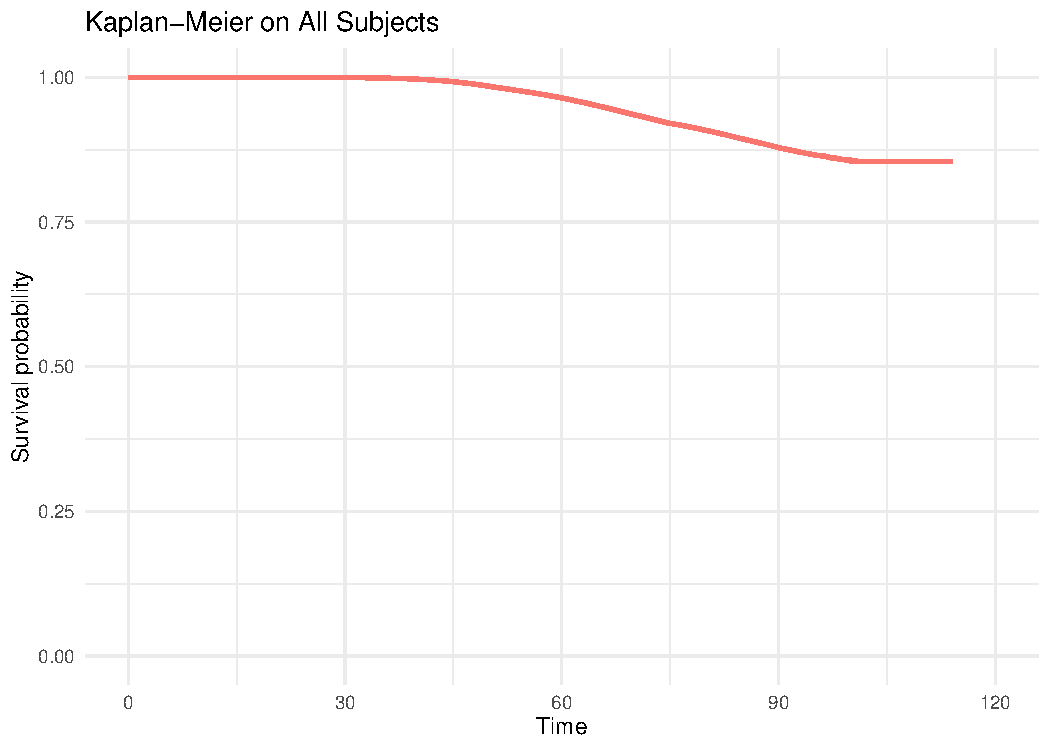
\includegraphics[width=\linewidth]{plots/Rplot100.pdf}
    \caption{Kaplan-Meier survival estimate of age at onset (all subjects).}
    \label{fig:kmall}
\end{figure}
% code in sisters.R SWEDEN COMPUTER  

Let us turn to the parameter estimation step.

Notice that in each family, the main subject may or may have not survival information on the mother. The analysis is conducted both on those main subjects that has a recorded mother in the Multi-Generational Dataset and on all main subjects (with or without recorded mother in the dataset). Additionally, a preliminary analysis is conducted on the semiparametric models with o without reproductive covariates such as the parity indicator, the number of children, and the age at first child in categories (with a category for those who have not yet had a child) in Table \ref{tab:14} without giving so different results from the covariate-free scenario. We conduct only this preliminary analysis because it is the easiest and fastest. We plan to extend the study on the covariates also to the other models, and first of all in a simulation study. 
\clearpage
\subsection{Semiparametric models}
In Section \ref{sec5} three semiparametric models have been studied in simulation studies, and then the analysis has moved to the parametric scenario. Not surprisingly, based on the simulation results, the Multivariate Shared Frailty Cox (MSFCox) outperforms all others in terms of predictive accuracy, and also does it in the available dataset, with a concordance index of 0.965, which is significantly higher than the Univariate FH Cox (UFHCox) model (0.5150) and Time-varying version with 0.5036 of concordance (as reported in Table \ref{tab:13}).
When we select only main subjects with the complete information on the mother, the concordance almost reaches the maximum value, up to a 99\% of concordant pairs. This result is outstanding, and the advantage of using the multivariate model instead of only the easier $FH$ model is immediately observed. Indeed, the Constant $FH$ and Time-varying $FH(t)$ models perform poorly, as their prediction concordance is comparable to that of a random flipping of a coin. Equally to the simulation study results, in bold is reported the best result by scenario, say by box, and the best across all scenario is highlighted.  
% The posterior frailty distributions of both the MSFCox and the UFCox models on the dataset without covariates are shown in Figure \ref{fig:postfraildens}. 

% \begin{figure}[ht]
%     \centering
%     \includegraphics[width=0.7\linewidth]{plots/Rplot85.pdf}
%     \caption{Posterior frailty density from the multivariate model (in red) versus the prior (in blue).}
%     \label{fig:postfraildens}
% \end{figure}
% \newline

% The key information obtained from the inference step is the estimated frailty parameter from the multivariate likelihood. The complete analysis output is presented in Table \ref{tab:13}, with standard errors of the estimated coefficients shown in parentheses. The family history variable is included as both an end-of-follow-up indicator and a time-varying covariate, resulting in two versions of the FHCox model. Parameter estimation is performed on the entire dataset, as well as on a subset of subjects with at least maternal information and born between 1946 and 1974. Additionally, the analysis is repeated with the inclusion of covariates such as parity, number of children, and age at first child. Results of the estimated parameter values can be found in Table \ref{tab:14}.

% \begin{table}[ht]
%     \centering
%     \begin{tabular}{l|ccc}
%     \hline
%     Model & Estimated $\widehat{\theta}$ &$\widehat{\beta}_{FH}$ & Concordance \\ \hline
%     MSFCOx &1.327 &- &\textbf{0.965} (se = 0) \\
%     UFCox &200 &- &- \\ 
%     UFHCox &- &1.449 (0.0173) &0.515 (se = 0.001) \\ \hline
%     \end{tabular}
%     \caption{Frailty parameter, family history coefficient and concordance estimated for three models: Multivariate Shared Frailty Cox (MSFCOx), Univariate Frailty Cox (UFCox) and Univariate FH Cox (UFHCox) model.}
%     \label{tab:ouputreal}
% \end{table}

\begin{table}[ht]
    \centering
    \begin{tabular}{l|cccc} \hline
    &Survival information mother &$\widehat\theta$ &$\widehat\beta_F$ &C \\
    Multivariate &yes &1.3624 &- &\hl{\textbf{0.9968}} \\
    Univariate FH &&- &1.5372 &0.5021 \\
    Univariate FH(t) &&- &1.8017 &0.5042 \\ \hline
    Multivariate &no &1.327 &- &\textbf{0.9650} \\
    Univariate FH &&- &1.449 &0.5150 \\ 
    Univariate FH(t) &&- &1.8405 &0.5036 \\ \hline
    \end{tabular}
    \caption{estimated parameters and Harrell's concordance index C (last column) for the three semiparametric models.}
    \label{tab:13}
\end{table}
% Code \texttt{finalEstimation-cox-swemultireg-MVV} in the Swedish VDI.

In Table \ref{tab:14} we report results from including the available reproductive covariates parity and number of children. No significant differences in terms of concordance index is noticed in comparison to the scenario without covariates.
\begin{table}[ht]
    \centering
    \begin{tabular}{l|cccc} 
    \hline
    &Survival information mother &$\widehat\theta$ &$\widehat\beta_F$ &C \\
    Multivariate &yes &2 &- &\textbf{0.9335} \\
    Univariate FH &&- &1.3922 &0.6209 \\
    Univariate FH(t) &&- &2.2254 &0.5350 \\ \hline
    Multivariate &no &2 &- &\hl{\textbf{0.9436}} \\
    Univariate FH &&- &1.3922 &0.5965 \\ 
    Univariate FH(t) &&- &1.8049 &0.5184 \\ \hline
    \end{tabular}
    \caption{estimated parameters and Harrell's concordance index for the three semiparametric models with parity, number of children, age at first child covariates.}
    \label{tab:14}
\end{table}
Also, we can not conclude anything about parameter recovery but the estimate of the frailty parameter $\widehat\theta$ in the second column of Table \ref{tab:13} has a reasonable value. Additionally, the estimated of the family history coefficient $\widehat\beta_F$ has a positive value (around 1.8) meaning that the family history has a positive effect on the breast cancer development, that is indeed coherent with this phenomenon.  
% Code \texttt{finalEstimationCovariates-cox-swemultireg-MVV} in the SWEDISH COMPUTER.
\newpage
% Code in ParContinuousFrailty-multivariate-swemultireg-MVV.R in the SWEDISH COMPUTER for the estimation of parameters and ParContinuousFrailty-multiunifh-postprediction-swemultireg-MVV.R for concordance with adjustement on the parameter values.  
We then use the estimated parameters to perform posterior prediction of familial frailty. Firstly, we apply the posterior prediction to the subjects in the initial dataset. Secondly, we perform an in-sample validation to assess the accuracy of the prediction. This involves defining a training and a validation set by conducting a in-sample validation. 
% Specifically, we remove one family at a time, fit the model on the remaining (n - 1) families, and predict only on the excluded family using the previously estimated parameters.

In other words, the algorithm takes as input the familial survival data of the female family members of a new woman. By providing information on her mother and sisters, the algorithm produces three quantities: the posterior mean frailty, the probability of belonging to the highest-risk group (top 5\%), and an indicator of whether the woman belongs to the highest-risk families compared to the population distribution of the probability of belonging to the highest-risk group, based on a fixed threshold. For example, from the semiparametric multivariate model we obtain that $\widehat{\theta} = 1.327$, and $\widehat{r}_{(1-\alpha)}$ is $0.1512$ for $\alpha = 0.05$. This means that if a woman has a probability of belonging to the highest-risk families over 15.12\%, then her indicator will take value one. We can determine whether the woman should be targeted, e.g., for a more careful treatment path with more intensive screening, surveillance, and other prevention strategies. This prediction can be made quickly and easily using the estimated frailty parameter, the (1-$\alpha$) percentile value, and the Breslow estimates of the cumulative hazard function obtained by fitting the multivariate model. These values can be stored for later use, enabling fast prediction without having to recompute the entire process for new women. This algorithm has been developed based on the model chosen in Section \ref{sec5}.

In Table \ref{tab:17}, a summary of the distribution of the cumulative hazard function is provided, specifically in the semiparametric scenario, and a plot of the cumulative hazard function is in Figure \ref{fig:8}, and its density from the entire population is reported in Figure \ref{fig:9}. Interestingly, we can notice how it can be split into two regions. It is worth noting that in the parametric scenario, the population parametric distribution provides more information and therefore there is no requirement for computing the nonparametric estimates of the cumulative hazard function and the quantile threshold. It is straightforward to extend this procedure to other percentile levels, although this necessitates refitting the model from the beginning, which can be time-consuming, nut we are certain that we can compute it for once and store it for later use. 
\begin{table}[ht]
    \centering
    \begin{tabular}{ccccccc}
    \hline
    Min. &1st Qu. &Median &Mean &3rd Qu. &Max. &NA's \\ 
    0.0000  &0.0000 &0.0324 &0.0752 &0.1389 &0.2583 &360 \\ \hline
    \end{tabular}
    \caption{estimated population Breslow cumulative hazard function summary on a grid of time values.}
    \label{tab:17}
\end{table}
\begin{figure}
    \centering
    \includegraphics[width=\linewidth]{PhD_thesis_template/plots/Rplot107.pdf}
    \caption{estimated Breslow cumulative hazard function.}
    \label{fig:8}
\end{figure}
\newpage
\begin{figure}
    \centering\includegraphics[width=\linewidth]{PhD_thesis_template/plots/Rplot102.pdf}
    \caption{density plot of the cumulative hazard function estimated from the entire population in object.}
    \label{fig:9}
\end{figure}
\newpage
An example is reported below for a woman with a family survival information as follows. Observed ages = (45, 90, 60) in years, and indicators of having observed the onset event = (0, 1, 0). Consider the first subject to be the woman who shows up at the hospital at 45 years of age, with the mother who had breast cancer onset at 90, and a sister who has not experienced the onset yet at age 60. The output from the algorithm is given by the following, which means that the woman does not belong to the highest-risk families: \\
\begin{verbatim}
    Posterior mean frailty = 1.5762
    Posterior median frailty = 2.7801
    Posterior high-risk probability = 0.1264
    Posterior high-risk membership = 0
\end{verbatim}
% Code with name \texttt{postPredictionReal1Family} and in Appendix \ref{appendix:b}. 
The significance of the observed times and breast cancer onset indicators on the probability of belonging to the highest-risk group is thus established. 

\subsection{Focus on the cure-rate}
The rich Swedish dataset also provides us with a precious opportunity to explore the debated issue of whether a cure-rate structure is reasonable in models for breast cancer onset. 

In order to evaluate the goodness of fit of the cure-rate structure for this dataset we now move to the parametric scenario and explore some parametric baseline survival function. Notice that this analysis gives some qualitative support to the hypothesis that a cure-rate exists, thus the frailty quantity here is not involved yet. We examine five distributions, namely Weibull, Gamma, Lognormal, three-parameters Gamma, and three-parameters Lognormal. We explore the multivariate and the univariate setting, fitting both the multivariate and the univariate multiplicative Lehmann frailty cure-rate and non-cure-rate models. Recall that in the univariate model, we only consider the survival information of the main subject per family, while in the multivariate model we consider all of the family survival information.

Results from the analysis are presented in Table \ref{tab:10}, where the models are compared using the Akaike Information Criterion (AIC) that is exactly \[
AIC = -2 n_{\pi} - \ln L(\pi),
\] with $n_\pi$ the dimension of the parameter collection, and $L(\pi)$ the likelihood on the parameters. It should be noted that the models are not nested. We compare the fit across models and between the cure-rate and non-cure-rate survival structure but always within the multivariate and the univariate cases (which also have very different sample sizes). The Multivariate Cure-Rate three-parameters Lognormal model yields the best result, with an AIC value of 1687555, while the regular Lognormal distribution provided the best performance for the Univariate Cure-Rate model with an AIC of 438368.4. 
\begin{table}[ht]
\centering
\begin{tabular}{l|cccc} 
\hline
% &\multicolumn{2}{c}{Multivariate model} &\multicolumn{2}{c}{Univariate model} \\
% \cline{2-5}
% &\multicolumn{2}{c}{AIC} &\multicolumn{2}{c}{AIC} \\
Multivariate &non-cure &cure \\ % &non-cure &cure \\ \hline
Weibull &1705353 &1692822 \\ 
Gamma &1698245 &1688066 \\ 
Lognormal &1693854 &2334626 \\ 
Gamma 3-parameters &1707589 &1687749 \\
Lognormal 3-parameters &1698257 &\textbf{1687555} \\ \hline
Univariate \\ 
Weibull &440685.6 &439053.4 \\ 
Gamma &439516 &438391.8 \\
Lognormal &438958.8 &\hl{\textbf{438368.4}} \\ 
Gamma 3-parameters &444890.7 &438386.2 \\
Lognormal 3-parameters &439460.9 &438369 \\ \hline
\end{tabular}
\caption{AIC comparison among different distributions, where in bold are the best results column-wise and according to the fitted model.}
\label{tab:10}
\end{table}
% Code in oneGroupGamma.R, oneGroupLogNormal.R, oneGroupWeibullNecessary.R in SWEDISH COMPUTER

All the curves shown in Figures \ref{fig:1.13}, \ref{fig:1.14}, and \ref{fig:1.15} support the hypothesis of a cure-rate model and show good closeness to the observed survival distribution better with the cure-rate estimated survival than the non-cure estimated survival function. Indeed, the cure-rate model seems to fit the data (until the end of the follow-up) better than the non-cure-rate models. From results, the cure-rate models are always preferred to the non-cure-rate models (except for the case of multivariate Lognormal model).

It is interesting to notice that support to the cure-rate structure is mainly given by the graphical analysis of the survival function of the mothers, due to their older ages: in Figure \ref{kmsisters}, the Kaplan-Meier curves by subjects (the main subject, the mother, and from the first sister to the last one) show that the tail of the Kaplan-Meier estimator and of the fitted cure-rate models (Figure \ref{fig:1.13}, \ref{fig:1.14}, \ref{fig:1.15}) is mostly attributable by the mothers (in black). A deepening about the reliability of the cure-rate structure and the heavy tail due to the presence of the oldest mothers is in Appendix \ref{appendix:1.e}. We do not find particular graphical differences in curves among the daughters, as it should be expected since the main subject is randomly sampled among all the sisters and so it is the ordering of the sisters. We do not consider in this graphical analysis the last sisters (the twelfth) because of the very limited number of subjects. We note here that one might extend the models to allow for a (say, polynomial) effect of birth cohort on the survival distribution and make distinction between the mother and the sisters.
\begin{figure}
    \centering
    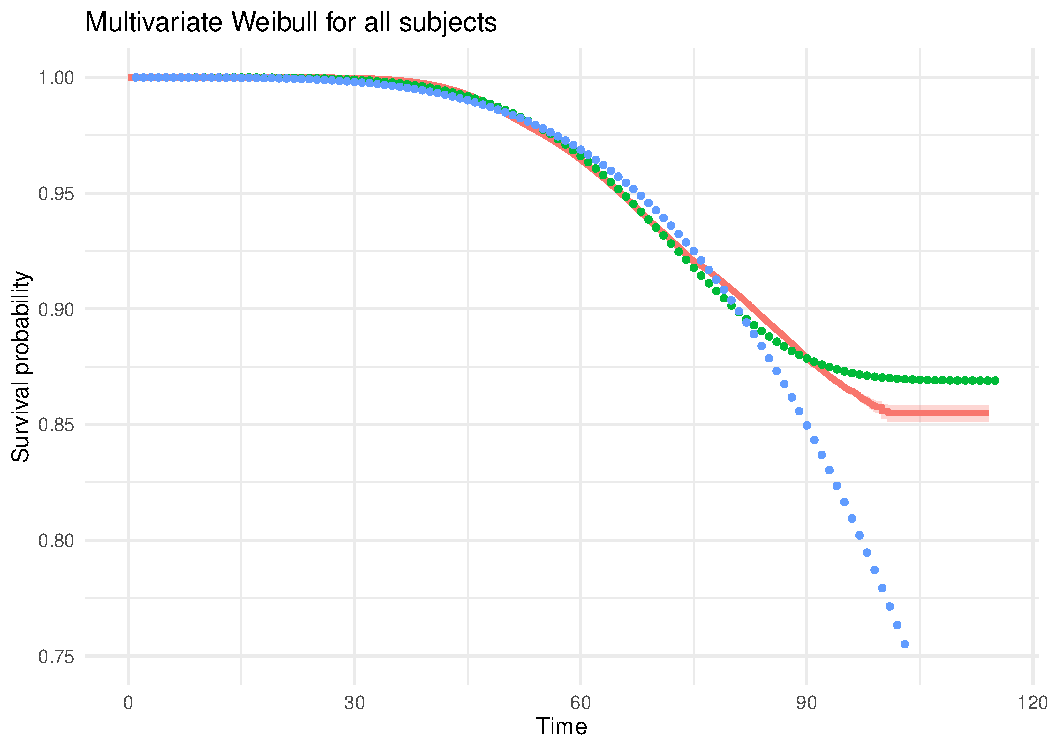
\includegraphics[width=\linewidth]{PhD_thesis_template/plots/Rplot108.pdf}
    \includegraphics[width=\linewidth]{PhD_thesis_template/plots/Rplot109.pdf}
   \caption{Kaplan-Meier for all subjects, in comparison to the estimated survival curves following the cure-rate (green) and the non-cure survival structure (blue) with Weibull and Gamma baseline survival function, on top and above, respectively.}
    \label{fig:1.13}
\end{figure}
\newline
\begin{figure}
    \centering
    \includegraphics[width=\linewidth]{plots/Rplot111.pdf}
        \includegraphics[width=\linewidth]{plots/Rplot112.pdf}
    \caption{Kaplan-Meier for all subjects, in comparison to the estimated survival curves following the cure-rate (green) and the non-cure survival structure (blue), with Lognormal and three-parameters Lognormal survival function, on top and above, respectively.}
    \label{fig:1.14}
\end{figure}
\newline
\begin{figure}
    \centering
    \includegraphics[width=\linewidth]{plots/Rplot110.pdf}
    \caption{Kaplan-Meier for all subjects, in comparison to the estimated survival curves following the cure-rate (green) and the non-cure survival structure (blue), with a three-parameters Gamma baseline survival function.}
    \label{fig:1.15}
\end{figure}
% Code for these plots is in: KMSubjectsMothers_Ultracentenary.R in the Swedish computer. 
\newline
\begin{figure}[ht]
    \centering
    \includegraphics[width=\linewidth]{plots/Rplot106.pdf}
    \caption{Kaplan-Meier of daughters, included the main subject, and mother (in black).}
    \label{kmsisters}
\end{figure}
% code in sisters.R SWEDEN COMPUTER 
\clearpage

However, on top of the AIC values, we are interested in the accuracy of the models to describe the observed cure-rate structure. 

We report the values of the estimated parameters in Table \ref{tab:1.17} and \ref{tab:1.18}. We run the analysis both on main subjects with reported survival information on the mother and on all main subjects (with the Weibull distribution fixed as the baseline survival distribution). In Table \ref{tab:1.18} we compare different baseline survival distribution on all the main subjects. Notice that we can not assess the model fitting accuracy by comparing the estimated parameters value with true values, because we are with a real dataset, but the estimated cured fraction value has a reasonable value for this specific application in the range, for example for $\widehat p$ in the first column of Table \ref{tab:1.17}, around 87\%-96\%. In Tables also the estimates of the baseline survival distribution parameters are reported, that are $\widehat shape_0$, and $\widehat scale_0$ for the Weibull and Gamma, with the addition of $\widehat\gamma_0$ for the threshold parameter in the three-parameters Gamma; $\widehat\mu_0$, and $\widehat\sigma^2_0$ for the Lognormal, with the addition of $\widehat\gamma_0$ for the threshold parameter in the three-parameters Lognormal. The frailty parameter $\widehat\theta$ and the $FH$ coefficient $\widehat\beta_F$ are reported in the same column for a matter of space, because also notice that each model estimates one or the other. 
\begin{table}[ht]
    \centering
    \begin{tabular}{l|cccccc} \hline
    &Survival info mother &$\widehat p$ &$\widehat{shape}_0$ &$\widehat{scale}_0$ &$\widehat\theta$/$\widehat\beta_F$ &C \\
    Multivariate &yes &0.8710  &6.2645 &73.2018  &4.9053 &\textbf{0.9592} \\
    Univariate &&0.9594 &0.1246 &0.1900 &1.2150 &0.3952 \\
    Univariate FH &&0.9635 &0.0926 &0.0394 &1.2174 &- \\ \hline
    Multivariate &no &0.8703  &6.1822 &72.9776  &4.3569 &\hl{\textbf{0.9663}} \\
    Univariate &&0.9750 &0.1176 &0.1193 &1.2614 &0.3963 \\  
    Univariate FH &&0.9658 &0.0965 &0.0362 &1.1982 &- \\ \hline
    \end{tabular}
    \caption{estimated parameters and concordance index for the three parametric models.}
    \label{tab:1.17}
\end{table}
% Code in ParContinuousFrailty-multidistribution-multivariate-swemultireg-MVV.R, ParContinuousFrailty-multidistribution-univariate-swemultireg-MVV.R, ParContinuousFrailty-multidistribution-univariate-fh-swemultireg-MVV.R in the SWEDISH COMPUTER for the estimation of parameters and ParContinuousFrailty-multiunifh-postprediction-swemultireg-MVV.R for concordance with adjustement on the parameter values.  
\begin{table}
    \centering
    \begin{tabular}{l|cccccc} \hline
    Multivariate &$\widehat p_0$ &$\widehat\mu_0 / \widehat{shape}_0$ &$\widehat\sigma^2_0 / \widehat{scale}_0$ &$\widehat\gamma_0$ &$\widehat\theta$/$\widehat\beta_F$ &C \\
    Weibull &0.8703  &6.1822 &72.9776 &- &4.3569 &\textbf{0.9663} \\ 
    Gamma &0.8552 &18.6981  &3.8617 &- &5.4790 &\textbf{0.9663} \\ 
    Lognormal &0.8419 &4.2911 &0.2604 &- &5.5265 &\textbf{0.9392} \\ 
    Gamma 3-pars &0.8529 &18.6685 &3.8172 &0.1546 &5.8116 &\hl{\textbf{0.9679}} \\
    Lognormal 3-pars &0.8408 &4.2746 &0.2590 &2.7922 &5.9126 &\textbf{0.9663} \\ \hline
    Univariate \\
    Weibull &0.9750 &0.1176 &0.1193 &- &1.2614 &0.3963 \\ 
    Gamma &0.8626 &5.9127 &11.5267 &- &-5.8713 &0.3963 \\ 
    Lognormal &0.6607 &4.5317 &0.3784 &- &1.4119 &0.5105 \\ 
    Gamma 3-pars &0.3250 &9.5974 &11.0534 &3.1358 &-1.4014 &0.4461 \\
    Lognormal 3-pars &0.2527 &4.8125 &0.4431 &11.5269 &2.0759 &0.49 \\ \hline
    Univariate FH \\
    Weibull &0.9635 &0.0926 &0.0394 &- &1.2174 &- \\ 
    Gamma &0.9590 &22.0724  &2.5169 &- &-1.1910 &- \\ 
    Lognormal &0.9774 &2.6356 &0.9717 &- &-3.0954 &- \\ 
    Gamma 3-pars &0.7076 &11.8656 &6.9557 &0.5153 &0.7802 &- \\
    Lognormal 3-pars &0.5237 &4.6639 &0.4117 &7.9716 &2.0892 &- \\ \hline
    \end{tabular}
    \caption{estimated parameters through the maximization of the multivariate, univariate likelihood or univariate likelihood with inclusion of family history as covariate, with baseline survival distribution varying.}
    \label{tab:1.18}
\end{table}
% codice su server meb: ParContinuousFrailty-multidistribution-multivariate-swemultireg-MVV.R, ParContinuousFrailty-multidistribution-univariate-swemultireg-MVV.R, ParContinuousFrailty-multidistribution-univariate-fh-swemultireg-MVV.R and ParContinuousFrailty-multiunifh-postprediction-swemultireg-MVV.R for concordance with adjustement on the parameter values. 
%  code for concordance multi-uni-unifh is in prova-concordance-2.R SWEDEN 

The conclusion coincides to the one in the semiparametric scenario. The multivariate model outperforms the other two univariate models compared in terms of prediction accuracy through the Harrell's concordance index C, reported in the last column of Tables \ref{tab:1.17}, and \ref{tab:1.18}. It has indeed around the 96\% of concordant pairs. Also, in comparison to the semiparametric scenario we can say that the estimated frailty parameter has a higher value in the multivariate parametric scenario bringing to assess that the frailty distribution here has a higher variance and thus this brings to an easier distinction among low-risk and higher-risk families, than the semiparametric scenario. 

Now we can predict the posterior family-specific frailty as shown in Section \ref{sec:1.6}. We compute the mean, median and mode of the posterior frailty distribution for each family. Later, we compute the posterior high-risk probability and the posterior high-risk membership indicator, fixed a frailty mean threshold. Here, too, we can also compute the whole estimated family-specific survival distribution, conditionally on the family survival information. For each woman we can compute thus, as in the semiparametric scenario, all the interesting quantities to assess whether to address her to prevention strategies targeted for highest-risk families. 
\newpage

\section{Discussion}\label{sec:1.7}
This study aims to contribute to the study of risk prediction models for breast cancer to better understand the nature and modeling of family-specific risk of onset. We consider the cure-rate structure as a realistic approach for the Swedish Multi-Generational Breast Cancer registry, where around the 85$\%$ of subjects have not experienced yet breast cancer onset within the observed follow-up. We thus extend the traditional proportional hazards assumption in this Lehmann family formulation to cure-rate models. We explore parametric (Gamma shared frailty) models in this cure-rate setting, as well as semiparametric models that do not assume the cure-rate structure. 

Although family information is crucial for risk prediction models for breast cancer, using only a summary of this information may not have enough predictive power, as it proved with the often used family history indicator (baseline covariate, or time-varying covariate). Our simulation-based comparison shows that a full multivariate framework induces much better performance in terms of accuracy in risk prediction, when only involving family membership without additional subject-specific covariates. A full assessment of the added value of the full multivariate model will clearly emerge when additional analyses can be conducted on other dataset. Including family-specific covariates can enhance precision in targeting and improve accuracy in identifying the frailty parameter, as well as classifying families into risk groups. Therefore, incorporating family-specific covariates is an intriguing extension worth exploring.

We believe that this work stands out among the others known in the literature as it improves several aspects of breast cancer risk prediction models. We report a deep comparison between our model and the BOADICEA model, that is one of the most powerful in this context. 

The BOADICEA model is based on a multiplicative hazard function that depends on a genetic frailty component. This approach consists of inferring a genetic latent quantity, the polygenic risk score (PRS), for predicting cancer risk based on the family history of the disease and other risk factors. The PRS is a weighted combination of single nucleotide polymorphisms (SNPs), which are genetic mutations, commonly spread into the population, that singularly give a small contribution to increase the risk of breast cancer, but that can be dangerous when combined all together.

The BOADICEA model is then univariate and based on the subject-specific hazard function \[ \lambda(t\mid r) = \lambda_0(t)exp(\beta(r)), \] as described in detail in several publications (\cite{antoniou2002comprehensive}, \cite{antoniou2004boadicea}, \cite{antoniou2008boadicea}, and \cite{thomas2004statistical}). It evaluates the likelihood function through a complex segregation analysis provided by the Mendel software \cite{lee2019boadicea}. 

In contrast, our proposed frailty model differs from the BOADICEA model (or other possible similar models) in several ways. While BOADICEA uses a subject-specific hazard within a univariate framework and infers a genetic latent quantity, our model works in a fully multivariate framework and we infer a generic risk latent quantity, i.e. the subject-specific polygenic score. We incorporate survival information in a family-specific hazard, while the BOADICEA hazard function is subject-specific and does not account explicitly for the family structure through the estimated genetic frailty component. Our model wins in the simplicity that it has involving only familial breast cancer information and no other factors such as genetic, as BOADICEA does. Nevertheless, it is not difficult to extend our work to the use of additional  covariates. The simplicity is also extended to the use of a full likelihood or partial likelihood maximization algorithm for parameter estimation, while BOADICEA relies on a complex segregation analysis to predict the PRS (specifically its variance).

Last but not least, at contrary to the BOADICEA model, we introduce the explicit cure-rate structure on the survival function, that is crucial when especially dealing with breast cancer risk prediction models.

Talking about possible extensions of our work, one could be the use of alternative frailty distributions, such as the Lognormal \cite{duchateau2008frailty}. Or, one could address the problem within the Bayesian framework \cite{karamoozian2021bayesian}. One could also compare the prediction accuracy between our multivariate -- semiparametric and parametric -- model and the BOADICEA model, but it would be necessary the access to the same complete dataset \cite{lee2017differences}.

% The method with the multivariate model is able to identify higher-risk families to address them to targeted screening surveillance and prevention paths.

% The family information has been proved to be crucial to gain more information on the risk of having breast cancer. The Univariate model has been proved to be not useful for this topic. The model is not identifiable so far, without the inclusion of valid familiar covariates. Of course this work can be readily extended to the use of covariates and compare again the multivariate model with the univariate to assess whether the available covariates could be useful for knowing the familiar risk to breast caner. The issue with this dataset is that we have not precise familiar information, but we can build some as the number of people in the family or the number of sons. 

% Unfortunately all the families are from Sweden and they are registered as Swedish citizen so we can not distinguish among countries. Also other information are equivalent over all the families and indeed not useful. Without covariates, the multivariate model not only performs better than the univariate model because it uses the survival family information but also it is more powerful than the family history indicator in terms of prediction accuracy. The family history indicator uses as well the family information but in a simplistic way, indeed we can appreciate, through this study, the huge advantage in using the extended family information instead of just a summary. 

% The adjusted mean results to be correlated to the real frailty in the simulation studies, but the summary error index related to the regular mean is always lower according the every family size maximum/minimum. This means that we prefer to use an index that is closer to the real frailty, and indeed the mean is used in the application. 

% There is shrinkage towards one when the expected number of events is very low. There a large amount of shrinkage in the cure-rate model when the families have few members within. It is interesting to study the behaviour of the posterior estimator of the frailty close to zero because the shrinkage is heavily towards the mean in our case. 

% compile first the main.tex, then run Bibtex on Chapter1.bib, Chapter2.bib and Chapter3.bib, finally compile main.tex again twice
\clearpage
\renewcommand{\bibname}{References}
\bibliographystyle{apalike}
\bibliography{biblio}

\chapter{A binary Frailty Cure-Rate model for age at disease onset}{In progress}
\markboth{\textsc{A binary Frailty CR model for age at disease onset}}{\textsc{A binary Frailty CR model for age at disease onset}}\label{chapter:2}

\begin{abstract}
We are interested on a specific aspect of survival modeling, namely the investigation of family-specific risk with a particular emphasis on the genetic component present from birth, as opposed to the environmental component. We assume that the true genetic family risk is latent and remains constant from birth, that we call ``frailty''. We focus on breast cancer development, even though this work can be extended to similar diseases. Our goal is to estimate this true family risk, as assessing the risk is crucial in improving individual survival chances by tailoring screening and prevention strategies to each individual's risk level. To achieve this goal, we employ a frailty model on the time to breast cancer onset, using a binary risk classification to split families into a low-risk group and a high-risk group. We compare this model to one that uses a strong risk factor, the family history indicator, to replace the latent binary risk. While the family history indicator solves the issue of latency, it is a weaker indicator of the complete detailed breast cancer familial history. 

\textbf{keywords}: breast cancer, family history, frailty models, survival analysis
\end{abstract}


\section{Introduction}
In 2020, female breast cancer overtook lung cancer as the most common cancer in the world. An estimated 2.3 million new cases of breast cancer were reported, constituting 12\% of all new cancer cases and 25\% of female cancer cases. Breast cancer ranked 5th in mortality, with 6.9\% among all cancer deaths, remaining the most common cause of cancer death in women (16\%). For example, in the USA the $12\%$ of women are estimated to experience breast cancer in their lifetime (see \cite{waks2019breast}), while in Sweden is the 9.4\% before age 75 \cite{strandberg2022breast}.

To tackle this problem, we want to use risk prediction models for breast cancer to identify families with the highest risk of developing breast cancer and provide them with targeted and more intensive screening and prevention strategies. Indeed, classifying subjects into risk groups allows for the modification of screening schedules (more/less intensive) depending on the risk of breast cancer for a given woman, for the implementation of additional prevention efforts, and for the reduction of unnecessary medical treatments, costs and psychological stress \cite{pepe2003statistical, skates2001screening}.

Remarkable contributions to the breast cancer risk modeling field include the Gail model (refer to \cite{gail1989projecting}), which employs logistic regression to integrate risk factors, such as the number of first-degree relatives with breast cancer, with the aim to compute the long-term probability of developing breast cancer. The Tyrer and Cuzick (TC) model, which (refer to \cite{tyrer2004breast}) integrates personal risk factors and complete genetic analysis (involving also BRCA1 and BRCA2 gene mutations) to model the risk of developing breast cancer by combining the genetic and familial components. The Rosner and Colditz model, which (refer to \cite{rosner2008risk}) is based on a logistic model for incidence that is affected by reproductive risk factors, including age at menarche, age at menopause, and age at childbirth. These models have been implemented in various studies, such as those described in \cite{darabi2012breast} and \cite{evans1996fictitious}. Models for disease onset also include the popular two-hit Moolgavkar-Venson-Knudson (MVK) cell-splitting model, which has all subjects eventually experience the disease, if right censoring does not intervene to end the observation of the time-to-event \cite{moolgavkar1979two}.

As we can observe from literature the inclusion of strong risk factors associated to breast cancer are commonly used into risk prediction models. One among the strongest risk factors (such as BRCA1, BRCA2, TP53, and SNPs, mammography density (MD) and body mass index (BMI) \cite{bravi2018risk}, \cite{lee2017differences}, \cite{strandberg2019statistical}, \cite{strandberg2022estimating}), the family history, is still involved in risk prediction models although we believe it is a weak indicator since it only provides a summary of the clinical history experienced by a family. Specifically, it is defined as the collection of breast cancer experiences within a family and is represented as a binary variable that takes a value of one when at least one family member has experienced breast cancer onset, and zero if none has. For comprehensive and complex data, family history may not fully capture the familial aggregation of breast cancer development.

On the other hand, the family history indicator motivates the binary nature of the breast cancer risk which leads to the split of families into a low-risk group and a highest-risk group. Thus, our objective is to develop a risk prediction model for age at breast cancer onset, say the beginning of the disease, which involves a family-specific risk assumed to be latent and unchanged from birth. Drawing inspiration from the family history indicator, we allow for this latent risk, namely the frailty risk, to be discrete and comprise two risk levels (low and high), which we denote as 0 and 1, respectively. In the following, we explore a Univariate $FH$ Cure-Rate model, a Univariate frailty Cure-Rate model and a Multivariate frailty Cure-Rate model, where frailty is referred to the latent risk of breast cancer development, ``Cure-Rate'' refers to the peculiar survival function which allows for a fraction of the population to not experience breast cancer onset eventually, and the difference between ``Multivariate'' and ``Univariate'' stands in jointly modelling all the time-to-events of a family, in opposition to model only the time-to-event of one subject per family. We refer to ``main subject'' the member that we randomly select when moving from the multivariate to the univariate scenario, and also the one we compute the family history on, since the family history is a subject-specific characteristic and the model that comprises it is univariate as well. 

We seek to illustrate and quantify how family data can be better used to learn about family-specific risk of developing diseases by using such a multivariate survival model for disease onset instead of summary-based methods, as usually is easier and used in the literature. For example, we may use as summary the family history. 

Lastly, to provide a comprehensive assessment, we also implement a Univariate Cure Rate Frailty model to determine the significant loss of information incurred when subjects are viewed as not part of a family sharing the same risk of BC development. 

We introduce the univariate background of the Frailty Cure Rate model in Section \ref{sec:2.1}, the methods about the Multivariate Shared Frailty Cure Rate model in Section \ref{sec:2.2}. A comparison between the the univariate and the multivariate framework is run in Section \ref{sec:2.3}, and we close with some discussion in Section \ref{sec:2.4}. 

\section{Univariate model for age at disease onset}\label{sec:2.1}
\subsection{Latent Cure Rate survival models}
The Univariate Frailty model \cite{duchateau2008frailty} on the time-to-event $T = t$ allows the hazard function $\lambda(t\mid r)$ to have a particular form including the frailty risk $R$ which captures the unobserved heterogeneity among subjects. The hazard is given by 
\[
\lambda(t\mid \alpha(r  )) = \alpha(r)\lambda_0(t),
\] 
where $\lambda_0(t)$ is the baseline hazard function that can assume a parametric distribution with parameter collection $\theta$ or a semiparametric form. The quantity $\alpha(r)$ is a general function of the risk, that we may use in the linear form $\lambda(t\mid R = r) = r\lambda_0(t)$. 

The model can be extended to the inclusion of subject-specific covariates. In this case the frailty quantity explains the unobserved heterogeneity that the covariates are not able to capture. The hazard function is given by: \[
\lambda_j(t\mid R = r) =r\lambda_0(t;x_j),
\] 
where $x_j$ are the covariates of the $j$th subject. The shared frailty hazard function allows to define the frailty as a family-specific quantity. Thus, this specification is used with clustered data, as it is our case, where the shared frailty hazard function is given by:
\[
\lambda_{ij}(t\mid R = r_i) = r_i\lambda_0(t;x_{ij}),
\] 
with $x_{ij}$ the $i$th subject-specific covariates in the $j$th family. 

In the binary case, the latent quantity can be represented as $R = (0, 1)$, where typically the relation between the hazard functions is $\lambda_1(t) = \alpha\lambda_0(t)$. This assumption allows the hazard and survival functions of group ``0'' to coincide with the baseline functions, while $\alpha<1$ ensures coherence with the assumption of a highest-risk group in the population and thus we can rely on the assumption of proportional hazard. Therefore, we obtain: \begin{align*}
    &\lambda_0(t) = \lambda(t\mid R=0) = \lambda_0(t;x_{ij}), \qquad S_0(t) = S(t\mid R=0) = S_0(t;x_{ij}), \\
    &\lambda_1(t) = \lambda(t\mid R=1) =  \alpha \lambda_0(t;x_{ij}), \qquad S_1(t) = S(t\mid R=1) = [S_0(t;x_{ij}) ]^\alpha.
\end{align*}

Now, recall the Multivariate Shared Frailty survival model \cite{hougaard2012analysis} to describe modeling jointly the time-to-events in a family \cite{rodriguez2010multivariate}. We handle multiple time-to-event data by leveraging the assumption of conditional independence. For instance, consider the case where two women belong to the same family, resulting in dependent time-to-events. However, assuming conditional independence given the family (i.e. given the shared frailty risk), and letting $T_1 = t_1$ and $T_2 = t_2$ be the time-to-events of the two women in the family, and let $r$ denote the frailty value, the joint survival function factorizes given the risk, so that \begin{align*}
    S_{12}(t_1,t_2\mid R) \overset{T_1\perp T_2\mid R}{=} S_1(t_1\mid R)S_2(t_2\mid R),
\end{align*} where one therefore assumes conditional independence given the frailty term $R$. Recall that, if $R = 0$, we have \[
    S_{12}(t_1,t_2) = S_0(t_1)S_0(t_2),
\] while, if $R = 1$, we have \[
    S_{12}(t_1,t_2) = S_1(t_1)S_1(t_2) = [S_0(t_1)S_0(t_2)]^\alpha.
\] 

It is important to notice that this case can be immediately extended to more than two survival times per cluster sharing the same risk $R$. More generally, the marginal survival function for $n_i$ subjects per family is given by: \[
S_{1\dots n_i}(t_1,\dots,t_{n_i}) = h\prod_{j=1}^{n_i}S_0(t_j) + (1-h)\prod_{j=1}^{n_i}\left[S_0(t_j)\right]^\alpha,
\] with $h$ the probability of belonging to the low-risk group of families. 
% If $S_0(t)$ is specified parametrically, inference can be performed through the traditional numerical methods to maximize the observed data likelihood.

Now, given the nature of the phenomenon, not all women will experience breast cancer onset, regardless of how long they will live. Therefore, we rely on the cure rate survival function \cite{mota2022new}, which can be considered as a mixture of a proper survival function, which models the fraction of individuals who will experience the event, that we call the ``cases'' and a degenerate distribution, which models the fraction of individuals who will not experience the event, that we call the ``non-cases''. We define a ``proper'' survival function, the one that tends to 0 when the time-to-events tends to $+\infty$, such as $\lim_{t \to+\infty}S(t) = 0$, and has probability equal to one that the time-to-event can not assumes value $+\infty$, such as $P(T<+\infty) = 1$. 

Let $T$ indicate a non-negative time-to-event random variable, the survival function that defines a cure rate model takes the form: \[
S_0(t) = p_0 + (1-p_0)\widetilde{S}_0(t)
\] (see, e.g., \cite{bondi2023approximate}) with $\widetilde{S}_0(t)$ the proper survival function. Indeed, let the survival random variable $T$ be such that, conditionally on being a case, it is absolutely continuous, and let $\widetilde{f}_0(t)$ indicate the conditional density function of the cases corresponding to the proper survival function $\widetilde{S}_0(t)$. In contrast, the fraction $p_0$ is defined the ``cured fraction'', i.e. the fraction of the subjects who will never experience the event of interest, so that $T= \infty$ with probability $p_0$. Figure \ref{fig:cure_rate} shows the difference between a traditional (in blue) and a cure rate (in red) survival model on randomly generated data. 
\begin{figure}[ht]
        \centering
        \includegraphics[width=\linewidth]{plots/Rplot04.pdf}
        \caption{traditional survival function (in blue) vs. a cure rate survival function (in red).}
  \label{fig:cure_rate}
\end{figure}
% code: KM_code_right-MVV.R from local problem

The question of whether a cure rate model is appropriate for a given phenomenon can be addressed by noting that a traditional proper survival function can be seen as a special case of a cure rate model with $p_0=0$. In other words, allowing for a cure rate simply enlarges the set of available models, within which traditional survival functions are nested through such constraint. We believe that implementing a cure rate model is the right way to address this problem. 

% \begin{lem}
% If $S(t)$ follows a cure rate structure, then it does not admit a density with respect to the Lebesgue measure. 
% \begin{proof}
% Note that we have \begin{align}
%     \label{formula:lemma_1}
%     \lim_{t\to\infty}S(t)= \lim_{t\to\infty}(p+(1-p)\widetilde{S}(t))=p>0
% \end{align}
% Suppose that a density function $f(t)$ exists so that $S(t)=\lim_{t\to\infty}\int_t^\infty f(u)\text{d}u$ and $\int_0^\infty f(u)\text{d}u=1$. Then, we will prove that \begin{align*}
%     &\lim_{t\to\infty}{\int_{t}^\infty f(u)\text{d}u}=0 \\
%     &\lim_{t\to\infty}{\int_{t}^\infty f(u)\text{d}u} = \lim_{t\to\infty}{\int_{0}^\infty \mathbbm{1}(s\ge t)f(s)\text{d}s} 
% \end{align*}
% We apply the dominated convergence \cite{weir1973lebesgue}: \begin{align*}
%     &\text{since }\mathbbm{1}(s\ge t)f(s) \le f(s) \ \forall s\ge 0 \text{ and } \int_0^\infty f(s)\text{d}s=1; \\
%     &\Rightarrow \int_0^\infty \mathbbm{1}(s\ge t)f(s) \le \int_0^\infty f(s)\text{d}s = 1. \\
%     &\text{Then, } \lim_{t\to\infty}S(t) = \lim_{t\to\infty}{\int_{t}^\infty f(s)\text{d}s} = \lim_{t\to\infty}{\int_{0}^\infty \mathbbm{1}(s\ge t)f(s)\text{d}s} \\
%     &\qquad\qquad\qquad\quad\overset{\overset{DCI}{\downarrow}}{=} \int_{0}^\infty\lim_{t\to\infty} (\mathbbm{1}(s\ge t)f(s))\text{d}s=0,
% \end{align*}
% \end{proof}
% \end{lem}

% which contradicts formula \ref{formula:lemma_1}. Thus, as expected, a proper density function associated with a cure rate survival function does not exist. Indeed, the density function conditionally to the uncured rate proportion $f(t) = (1-p)\widetilde{f}(t)$ is improper, as the cure rate marginal density function.

Thus, we assume that there exist two latent risk classes: low (or ``general'') risk (R=0) and high-risk (R=1). Let $h=P(R=1)$. For the two risk classes one has $S_r(t) = p_r + (1-p_r) \widetilde{S}_r(t)$, with $r \in \{0,1\}$ (see Figure \ref{fig:2.2} from a trivial simulation study in \texttt{R}), such that \begin{align*}
&S_0(t) = p_0 + (1-p_0)\widetilde{S}_0(t) \\
&S_1(t) = [p_0 + (1-p_0)\widetilde{S}_0(t)]^\alpha = p_1 + (1-p_1)\widetilde S_1(t)
\end{align*}
\begin{figure}[ht]
    \centering
    \includegraphics[width=\linewidth]{plots/Rplot02.pdf}
    \caption{cure rate model with two latent risk groups.}
\label{fig:2.2}
\end{figure}
\newline
%qui
Suppose for now that the two conditional distributions $\widetilde{S}_0(t)$ and $\widetilde{S}_1(t)$ can be chosen freely, and that to them correspond two given densities $\widetilde{f}_0(t)$ and $\widetilde{f}_1(t)$ with (possibly vector) parameters $\theta_0$ and $\theta_1$, respectively. Thus the complete (vector) parameter for the model is $\underline\theta = (p_0, p_1, \theta_0^T, \theta_1^T, h)^T$.

Recall that the observed data $(\underline x=(x_1, x_2, \ldots, x_n)^T, \ \underline\delta=(\delta_1, \delta_2, \ldots, \delta_n)^T)$ is an i.i.d. sample of independently right-censored observed survival times from the population, where for the generic subject $i$, $x_{i}=\text{min}(t_{i}, c_{i})$, and $\delta_{i}=\mathbb{I}(t_{i} \le c_{i})$ following the usual notation that has $t_i$ indicate the survival time, where in our case is the age in years at breast cancer onset, and $c_i$ indicate the independent censoring time, both measured from the same origin. Without additional constraints, from the observed data $(\underline{x},\underline\delta)$ one may not identify the parameter vector $\underline\theta$. 

\subsubsection*{A note on non-identifiability}
When we talk about inference, we also want to deepen the topic of parameter identifiability. This argument is very interesting and not easy to manage in the case of two risk groups. Due to the complicate nature of this phenomenon, we explore different scenarios in the following lines as: (I) identifiability of the classical survival function $S_0(t) = \widetilde{S}_0(t)$; (II) identifiability of the cure rate survival function $S_0(t) = p_0 + (1-p_0)\widetilde{S}_0(t)$, with $\widetilde{S}_0(t)$ a proper survival function; (III) identifiability of the Lehmann structure $S_1(t) = [S_0(t)]^{\alpha(z)}$; 
% (IV) identifiability of the cure rate survival model $S_0(t) = p_0 + (1-p_0)\widetilde{S}_0(t)$; 
(IV) identifiability of the cure rate Lehmann structure $S_1(t) = [p_0 + (1-p_0)\widetilde{S}_0(t)]^{\alpha(z)}$; (V) identifiability of the marginal cure rate survival function $S(t) = (1-h)S_0(t) + hS_1(t)$. Notice that we generalize the form of $\alpha(z)$ to be in function of covariates $z$, but it may be also a constant. 

Trivially cases (I), (II), and (III) can be proved. The proof of case (IV) follows. 
\begin{proof}
\begin{align*}
    &S_1(t) = [p_0 + (1-p_0)\widetilde{S}_0(t)]^{\alpha(z)} = p_0^{\alpha(z)} + \left(1-p_0^{\alpha(z)}\right)\widetilde{S}_1(t;\alpha(z)) \\
    &[p_0 + (1-p_0)\widetilde{S}_0(t;\theta)]^{\alpha(z)} = [p_0 + (1-p_0)\widetilde{S}_0(t;\theta')]^{\alpha'(z)} \quad \forall z \\ 
    &\alpha(z)\log[p_0 + (1-p_0)\widetilde{S}_0(t;\theta)] = \alpha'(z)\log[p_0 + (1-p_0)\widetilde{S}_0(t;\theta')] \\ 
    &\underbrace{\dfrac{\alpha(z)}{\alpha'(z)}}_\text{not in function of t} = \underbrace{\dfrac{\log[p_0 + (1-p_0)\widetilde{S}_0(t;\theta)]}{\log[p_0 + (1-p_0)\widetilde{S}_0(t;\theta')]}}_\text{not in function of z} = c. 
\end{align*}
Since, \begin{align*}
    &\lim_{t\to\infty}\widetilde{S}_0(t;\theta) = 0, \ \lim_{t\to\infty}\log(p_0+(1-p_0)\widetilde{S}_0(t;\theta)) = \log(p_0) \Rightarrow c = 1 \\
    &\Rightarrow \alpha(z) = \alpha'(z). 
\end{align*}
Then also, \begin{align*}
    &\log[p_0 + (1-p_0)\widetilde{S}_0(t;\theta)] = \log[p_0 + (1-p_0)\widetilde{S}_0(t;\theta')] \\
    &\Rightarrow p_0 + (1-p_0)\widetilde{S}_0(t;\theta) = p_0 + (1-p_0)\widetilde{S}_0(t;\theta') \\
    &\Rightarrow \widetilde{S}_0(t;\theta) = \widetilde{S}_0(t;\theta') \\
    &\Rightarrow \theta = \theta'
\end{align*}
\end{proof}
That proved the identifiability of the cure rate Lehmann survival function, in the case where the baseline survival function $S_0(t;\theta)$ has a parametric distribution. 

The case (V) seems trickier than the other cases. The marginal survival function $S(t)$ can be expressed in terms of both the baseline $S_0(t)$ and the distribution of the frailty risk $R$. This relationship is determined through the moment generating function (MGF) of $R$ evaluated at the argument $\log \left( S_0(t) \right)$. Thus, the marginal survival function is given by
\begin{eqnarray*}
S(t) &=&    \mathbb{E}_R \left[ S_0(t) ^R   \right] = \mathbb{E}_R \left[{\rm e}^{ R \, \log(S_0(t)) }  \right] = MGF_R \left(  \log \left(S_0(t) \right) \right).
\end{eqnarray*}

As long as the integral converges, this form applies to many multiplicative frailty models. Recall that if $P(R \geq 0)=1$, the MGF coincides with the Laplace transform of the random variable $R$, evaluated at minus the argument.

Again, we structure the two-latent-class frailty model that has $R \in  \{0,1\}$ as a binary multiplicative frailty model, since under proportional hazards assumption the two hazard functions $\lambda_0 (t) = \lambda(t \mid R=0)$ and $\lambda_1 (t) = \lambda(t \mid R=1)$ are such that $\lambda_1(t) = \alpha \, \lambda_0(t)$ for the constant $\alpha=\lambda_1(t) / \lambda_0(t)$ for any $t$. As a consequence, the survival time $T$ has the two conditional survival distributions $S_0(t)=P(T \leq t \mid R=0)$ and $S_1(t) = P(T \leq t \mid R=1)$, and its distribution can be described as a multiplicative frailty model with frailty random variable $R$ such that $R = 1$ w.p. $P(R=1)=1-h$ and $R=1 \iff \alpha=\lambda_1(t) / \lambda_0(t)$ w.p. $P(R=r)=h$. For such a random variable the MGF is
\[
MGF_R (u) = \mathbb{E}_R(e^{ur}) = {\rm e}^{u} (1-h) + {\rm e}^{u\alpha} h = {\rm e}^u
+ \left( {\rm e}^{u\alpha} -{\rm e}^u \right)  h = e^u(1-h) + e^{u\alpha}\]
and as a consequence the marginal survival distribution of $T$ is equal to
\[
S(t) = MGF_R \left( \log(S_0(t)) \right) = {\rm e}^{\log ( S_0(t))} (1-h) + {\rm e}^{\log(S_0(t)) \alpha} = S_0(t) (1-h) + S_1(t) h.
\] where, recall, the two survival functions follow a cure rate structure, such that $S_0(t) = p_0 + (1-p_0)\widetilde{S}_0(t)$ and $S_1(t) = p_1 + (1-p_1)\widetilde{S}_1(t)$. At this point we obtain the complete form of the marginal survival distribution of $T$, without specifying the baseline survival function that can be fixed later. The model, which may be seen as a double mixture of survival function, is not identifiable unless some constraint is set. The two conditional distributions $\widetilde{S}_0(t)$ and $\widetilde{S}_1(t)$ can in principle be chosen freely, and let us assume that they follow two given parametric distributions with densities $\widetilde f_0(t)$ and $\widetilde f_1(t)$ with (possibly vector) parameters $\theta_0$ and $\theta_1$, respectively. Thus the complete (vector) parameter for the model is $\underline\theta = (p_0, p_1, \theta_0^T, \theta_1^T, h)^T$, as already defined above.

Let us ignore the presence of administrative right censoring, and therefore assume that all censored observations are all (and the only) ``non-cases.'' This is a case in which more information is available on the model parameters, since additional right censoring would reduce the information available on the ``cases.'' The generic contribution $l_i$ to the likelihood function by subject $i$ with observed data $(x_i,\delta_i)$ is
\[
L_i(\underline\theta; (x_i,\delta_i)) = \left[ (1-h)(1-p_0) \widetilde{f}_0(x_i) + h(1-p_1) \widetilde{f}_1(x_i) \right]^{\delta_i} \left[ (1-h)\,p_0+h\, p_1 \right]^{1-\delta_i},
\]
so that the likelihood function is equal to
\begin{align*}
&L(\underline\theta; (\underline x,\underline\delta)) = \prod_{i=1}^n L_i(\underline\theta; (x_i,\delta_i)) \\
&=\prod_{i \in cases} \left[ (1-h)(1-p_0) \widetilde{f}_0(x_i) + h(1-p_1) \widetilde{f}_1(x_i) \right]   \prod_{i \in non-cases} \left[ (1-h)\,p_0+h\, p_1 \right]  \\
&= \left\{ \prod_{i \in cases} \left[ (1-h)(1-p_0) \widetilde{f}_0(x_i) + h(1-p_1) \widetilde{f}_1(x_i) \right] \right\}  \left[ (1-h)\,p_0+h\, p_1 \right]^{n_{\infty}} , 
\end{align*}
with $n_{\infty}$ the number of non-cases in the data (and $n-n_{\infty}$ the number of cases).

Now, let $\beta_1=(1-h)(1-p_0)$; $\beta_2=h (1-p_1)$, and $\beta_3=(1-h)\,p_0+h\, p_1$. The likelihood function can be re-written as
\[
L(\underline\theta; (\underline x,\underline\delta)) = \left\{ \prod_{i \in Cases} \left[ \beta_1 \widetilde{f}_0(x_i) + \beta_2 \widetilde{f}_1(x_i) \right] \right\}   \beta_3 ^{n_{\infty}},
\]
where one can easily check that $\beta_1 + \beta_2 + \beta_3 = 1$, with all three terms positive.

The proportion $n_{\infty}/n$ of non-cases can estimate non parametrically the parameter $\beta_3$, and from it the quantity $1-\beta_3=\beta_1+\beta_2$. As a consequence, the term $\beta_1 + \beta_2$ is identified. If one then multiplies and divides the likelihood by the term $(\beta_1+\beta_2)^{n-n_{\infty}}$, it seems clear that the quantity $\beta_1/(\beta_1+\beta_2)$ (and thus also the quantity $\beta_2/(\beta_1+\beta_2)$) is also identified from the mixture terms in the curly bracket, which is based on the cases, together with the parameters $\theta_0$ and $\theta_1$ of the two density functions  $\widetilde{f}_0$ and  $\widetilde{f}_1$.

Therefore, the two parameters $\theta_0$ and $\theta_1$, as well as the two quantities $\beta_1$ and $\beta_2$, are identified. On the other hand, in general the individual parameters $h, p_0, p_1$ are not identified from the observed data.

Given the constraints $p_0 \in (0,1)$ and $p_1 \in (0,1)$, and the assumption that $p_0 > p_1$ (which is without loss of generality given the freedom of deciding which group is ``0'' and which is ``1''), from knowledge of the values of $\beta_1$ and $\beta_2$ one may rule out some regions of $(0,1)$ as possible values for $h$. Indeed, since $(1-p_0)= \beta_1 / (1-h)$ and $(1-p_1)= \beta_2 / h$, and noting that $p_0>p_1 \iff 1-p_0 < 1-p_1$, simple algebra shows that $h$ must fall in the interval $[\beta_2, \beta_2/(\beta_1+\beta_2) ]$. This in turn restricts the possible values that the pair $(p_0, p_1)$ can take, since $p_0=1-\beta_1 / (1-h)$ and $p_1 = 1- \beta_2 / h$. \hspace*{\fill} $\square$

As a consequence of this fact, one may try to place some constraints on the parameters to create identifiability. One example is the following restriction, associated with the hazard functions $\widetilde{\lambda}_0(t)$ and $\widetilde{\lambda}_1(t)$ for the two time-to-event distributions for the cases in the two groups:
\begin{eqnarray}
\frac{\widetilde{\lambda}_1(t)}{\widetilde{\lambda}_0(t)} = \frac{p_0}{p_1} = \frac{1}{\alpha},   \label{CCR}  % For Constrained Cure Rate model
\end{eqnarray}
thus imposing the PH structure on the distributions of the cases in the two groups, plus the assumption that the factor $\alpha \in (0,1)$ that relates $\widetilde{\lambda}_0(t) = \alpha \, \widetilde{\lambda}_1(t)$ is the same that relates $p_0$ to $p_1 = \alpha \, p_0$.

We call such model the Proportional Hazards Constrained Cure Rate (PHCCR) model. Notably, in the PHCRR model the higher-risk group is associated with both a larger fraction of cases and earlier age at onset for their disease.

Note that to achieve identifiability one may also try to impose prior distributions on the parameters. Or, one may perform a sensitivity analysis that replaces this restriction with a fixed value for $p_1/p_0 = \rho$. 

\subsubsection*{Example 1.} 
Let the two conditional distributions of the survival times of the cases be distributed as Exp$(\lambda_0)$ and Exp$(\lambda_1)$ respectively for the two risk groups, with $\lambda_1 > \lambda_0$, i.e. such that $\lambda_0 = \alpha \, \lambda_1$ with $\alpha \in (0,1)$. Note that we also have $p_1 = \alpha \, p_0$. 

The following output illustrates the PHCCR model with two exponential CR survival sub-models. The simulations are based on 1,000 simulated dataset of size n=100,000 individuals each.
\begin{table}[ht]
    \centering
    \begin{tabular}{l|cccc} \hline
    &$p_0$ &$l_0$ &$\alpha$ &h \\
    True value &0.8 &0.1 &0.3333 &0.8 \\
    Mean &0.7995 &0.1001 &0.3335 &0.7994 \\
    Se &0.0005 &0.0002 &0.0004 &0.0002 \\
    $\sqrt{MSE}$ &0.0220 &0.0051 &0.0152 &0.0059 \\ 
    95\% C.I. Lower &0.7981 &0.0998 &0.3326 &0.7991 \\ 
    95\% C.I. Upper &0.8008 &0.1004 &0.3345 &0.7998 \\ \hline
    \end{tabular}
    \caption{results on the identifiability of a two risk groups CR model with Exponential survival functions.}
    \label{tab:2.1}
\end{table}
\newpage

In Table \ref{tab:2.1} is reported the parameter recovery in mean and standard error of the estimated parameter values across the 1,000 repetitions; the square root of the mean square error $\sqrt{MSE}$, that represents a measure of the absolute distance between the true value from the data generation process and the estimated value from observed data. The $MSE$ is given by \[
MSE = \dfrac{1}{n}\sum_{i=1}^n(\widehat r_i - r_i)^2.
\] 

Also, the lower-bound and the upper-bound of the 95\% confidence interval (C.I.) are reported. 

\subsubsection*{Example 2.}
Let the two conditional distributions of the survival times of the cases be Weibull$(shape_0$, $scale_0)$ and Weibull$(shape_1, scale_1)$ respectively for the two risk groups, with $shape_0=shape_1$. To implement the conditional proportional hazards model $\widetilde{\lambda}_0(t)=\alpha \, \widetilde{\lambda}_1(t)$ one simply sets $scale_1 = scale_0 \, ( \alpha^{1/shape_0})$. Again, $p_1=\alpha \, p_0$ (easy to check).

\begin{table}[ht]
    \centering
    \begin{tabular}{l|ccccc} \hline
    &$shape_0$ &$scale_0$ &$shape_1$ &$\alpha$ &h \\
    True value &20 &65 &20 &0.70 &0.80 \\
    Mean &20.2413 &64.9588 &20.1350 &0.7006 &0.8000 \\
    Se &0.0360 &0.0088 &0.0185 &0.0001 &0.0004 \\
    $\sqrt{MSE}$ &1.1626 &0.2814 &0.6014 &0.0032 &0.0131 \\ 
    95\% C.I. Lower &20.0184 &64.9042 &20.0201 &0.7000 &0.7974 \\ 
    95\% C.I. Upper &20.4642 &65.0133 &20.2498 &0.7013 &0.8025 \\ \hline
    \end{tabular}
    \caption{results on the identifiability of a two risk groups CR model with Exponential survival functions.}
    \label{tab:2.1}
\end{table}

These two small examples confirm that the parameter values that are used to generate the data are recovered correctly by the maximum likelihood estimators, with only small residual biases for the estimators.

\subsection{A two-latent-class Lehmann Cure Rate model}
As an alternative to the PHCCR model, we now extend the definition of the Lehmann family of distributions to the case of cure rate models, still within the latent class framework.

Recall the Lehmann family of distributions is equivalent to the definition of the proportional hazards (PH) structure for proper survival distributions:
\begin{equation*}
\left\{  S_{\alpha}(t) = \left[ S_0(t) \right]^{\alpha}, \ \ \alpha >0  \right\},   
\label{formula:2.PH}
\end{equation*}
where $S_0(t)$ is the (proper) baseline survival function and the parameter $\alpha$ modifies it to become the (also proper) survival function $S_{\alpha}(t)$. Let all random variables in the family be absolutely continuous random variables. It is then easy to check that $\lambda_{\alpha}(t) = \alpha \, \lambda_0(t)$ for any choice of (positive and finite) $\alpha$.
Indeed, when $\alpha$ is modelled through a regression structure one has the celebrated semiparametric Cox proportional hazards (PH) survival model \cite{cox1972regression}.

Here, we suggest extending the PH model to the model defined by the more general { Lehmann cure rate} family obtained by applying the Lehmann power transformation to a baseline cure rate model:
\begin{equation*}
    \left\{  S_{\alpha}(t) = \left[ p_0 + (1-p_0) \widetilde{S}_0(t) \right]^{\alpha}, \ \ \alpha >0  \right\}.   
    \label{formula:2.LehmannCR}
\end{equation*}
For a fixed value $\alpha$, the survival function $S_{\alpha}(t)$ also defines a cure rate model. Indeed, $\lim_{t \rightarrow \infty} S_{\alpha}(t) = p_0^{\alpha}$, and $S_{\alpha}(t)$ can be written as
\[
S_{\alpha}(t) = p_0^{\alpha} + \left( 1-p_0^{\alpha} \right) \widetilde{S}_{\alpha}(t)
\]
with conditional (proper) survival function for the cases equal to
\[
\widetilde{S}_{\alpha}(t) = \frac{\left[ p_0 + (1-p_0) \widetilde{S}_0(t) \right] ^{\alpha} - p_0^{\alpha}}{1-p_0^{\alpha}}
\]
and conditional density function
\begin{eqnarray*}
\widetilde{f}_{\alpha} (t) = - \frac{d}{d t} \widetilde{S}_{\alpha}(t) = \frac{1-p_0}{1-p_0^{\alpha}} \alpha \left[ p_0 + (1-p_0) \widetilde{S}_0(t) \right]^{\left(\alpha -1 \right)} \widetilde{f}_0(t).   \label{conddens}
\end{eqnarray*}

We note that here, too, a regression model with $\alpha=\alpha(z)$ can also be constructed for a vector $z$ of observed covariates if they are available.

A two (or indeed more) latent class parametric Lehmann Cure Rate model can now be easily
defined. Recall the Lehmann structure on the survival function characterizing the risk group $S_r(t) = [S_0(t)]^{\alpha(r)}$, such that we have: \begin{align*}
    &S_0(t) = p_0 + (1-p_0)\widetilde{S}_0(t), &S_1(t) = [p_0 + (1-p_0)\widetilde{S}_0(t)]^\alpha.
\end{align*} For a fixed $\alpha$, also the high-risk survival function $S_1(t)$ defines a cure rate model. % We identify the latent risk as a parameter $\alpha$ to be estimated. The proportional hazard (PH) structure allows the hazard function in a risk group to be written in function of the baseline hazard $\lambda_0(t)$, such that $\lambda_r(t) = \alpha(r) \lambda_0(t)$ (in particular $\lambda_0(t)$, and $\lambda_1(t) = \alpha \lambda_0(t)$), where $\lambda_0(t)$ is distributed according to a parametric distribution identified by the parameter collection $\underline{\theta}$, or a semiparametric distribution. Hence, it follows that the survival function is identified by a Lehmann structure, such that $S_r(t)=[S_0(t)]^{\alpha(r)}$. We thus have $S_0(t)$, and $S_1(t) = [S_0(t)]^{\alpha}$. Recall that the baseline survival function is defined by the more general Lehmann  family obtained by applying the Lehmann power transformation to a  survival function $S_r(t) = \left[p_0 + (1-p_0) \widetilde{S}(t) \right]^{\alpha(r)}$, with $\widetilde{S}(t)$ a proper survival function, so that we have $S_0(t) = p_0 + (1-p_0) \widetilde{S}(t)$, and $S_1(t) = [p_0 + (1-p_0) \widetilde{S}(t)]^\alpha$. For a fixed value $\alpha$, the aforementioned model is such that the survival function $S_1(t)$ also defines a  model. 
It is easy to check that $\lim_{t \rightarrow \infty} S_{1}(t) = p_0^\alpha = p_1$, and that $S_1(t)$ can be written as
\[
S_1(t) = p_1 + \left( 1-p_1\right) \widetilde{S}_1(t),
\]
with conditional (proper) survival function for the cases equal to:
\[
\widetilde{S}_1(t) = \dfrac{\left[p_0 + (1-p_0) \widetilde{S}_0(t) \right] ^\alpha - p_0^{\alpha}}{1-p_0^{\alpha}},
\]
and conditional density function: 
\[
\widetilde{f}_1(t) = - \dfrac{d}{d t} \widetilde{S}_1(t) = \dfrac{1-p_0}{1-p_0^{\alpha}} \alpha \left[p_0 + (1-p_0) \widetilde{S}_0(t) \right]^{\left(\alpha -1 \right)} \widetilde{f}_0(t).   
\]

Since the cure rate survival function is not proper, the density function associated with the cure rate model is also not proper. Note that, without loss of generality, for $\alpha> 1$ one has $S_1(t) < S_0(t) \ \forall t > 0$ and $p_1 < p_0$.
Indeed, we may reparametrize $\alpha_1 = 1/\alpha\in(0, 1)$ to impose $\alpha > 1$. 

For example, if one assumes a survival function distributed according to the Exponential distribution $\widetilde{S}_0(t) = {\rm e}^{- \lambda_0 t}$ for the distribution of $(T \mid R=0, case)$, then
\[
\widetilde{S}_1(t) = \frac{\left[ p_0 + (1-p_0) {\rm e}^{-\lambda_0 t} \right] ^{\alpha} - p_0^{\alpha}}{1-p_0^{\alpha}},
\]
and
\[
\widetilde{f}_1(t) = \frac{\alpha ( 1 - p_0) \lambda_0}{1- p_0^\alpha}  \left[ p_0 + (1-p_0 ) {\rm e}^{-\lambda_0 t} \right]^{\alpha -1}  {\rm e}^{-\lambda_0 t}. 
\]

Interesting comments about the two-latent-class Lehmann Cure Rate model are in Appendix \ref{appendix:2.l}.

% For simplicity, we have not included the term related to the risk thus far. To incorporate the risk group, we can rewrite the survival function $S_r(t) = [S_0(t)]^r$ as a function that depends on the risk group. Therefore, the generalized model is expressed as:
% \begin{align*}
%     % S(T=t\mid R=r) = 
%     S_r(t) = S(T=t\mid R=r) = [S_0(t)]^r, \ r \in \{r_0,r_1\}.
% \end{align*} 
% Note that if $T\sim S_0(t)$, then $P(T=+\infty)=p>0$, and a proper density function $f_T(t)$ does not exist. 

\subsubsection*{Data generation from the two-latent-class Lehmann Cure Rate model}\label{fastdatagen}
In simpler models (ex. the Exponential and Weibull seen above), the generation of observations from the high-risk group is easy by analytical inversion of $\widetilde{S}_1(t)$ (for cases), after having generated the case/non-case status.

Splitting subjects into two risk groups, we have the closed form of the survival function on the observed time for cases into the low-risk and high-risk group. For the Exponential baseline survival function $\widetilde{S}_0(t) = \text{e}^{- \lambda t}$, and the Weibull survival function $\widetilde{S}_0(t) = \text{e}^{-(t/ \lambda)^{ k}}$, with scale $\lambda$ and shape $ k$ inverting the survival function brings to generating the time-to-events from, respectively, 
\begin{align*}
    &t = -\dfrac{1}{\lambda}log(u), &t = \lambda\log\left(\dfrac{1}{u}\right)^{1/ k}.
\end{align*}
where $u\sim\text{Unif}[0,1]$. Similarly, we obtain for an observation from $\widetilde S_1(t)$, where the time-to-event generation formula for Exponential and Weibull distribution is given by, respectively,  \begin{equation*}
    t = -\dfrac{1}{\lambda} \log \left( \dfrac{ \left[ (1-p_0^{\alpha}) u + p_0^{\alpha} \right]^{1/{\alpha}}-p_0}{1-p_0} \right), \qquad t = -\lambda\left[\log\left(\dfrac{[(1-p_0^{\alpha})u+p_0^{\alpha}]^{1/{\alpha}}-p_0}{1-p_0}\right)\right]^{1/ k}.
\end{equation*}

While this model is clearly appealing in its interpretation, it is difficult to identify its parameters. Thus, fitting of such latent model requires that one has additional external information on the value of some of the parameters. 

When the distribution $\widetilde{S}_0(t)$ is not as trivial as the -- typically not very useful -- Exponential distribution, generation of observations from the high-risk group requires inversion of the survival function $\widetilde{S}_1(t)$ through numerical integration from $\widetilde{f}_1(t)$, the conditional density function of the cases in the high-risk group. This allows to produce samples from the distribution.

However, a much faster and precise algorithm exists from the form of the marginal survival function for the high-risk group. One may generate values $u$ from the $U(0,1)$ distribution and invert $S_1(t)=[S_0(t)]^{\alpha}$ directly to produce the value $t=S_1^{-1}(u)$. One should produce the value $T=\infty$ whenever $u< p_1=p_0^{\alpha}$, and solve $u=S_1(t)$ for $t$ when $u \geq p_1$. It is easy to check that this yields
\[
t= \widetilde{S}_0^{-1} \left( \frac{u-p_0}{1-p_0}  \right)=\widetilde{F}_0^{-1}\left( \frac{1-u}{1-p_0} \right), \ {\rm and}\ t= \widetilde{S}_0^{-1} \left( \frac{u^{1/\alpha}-p_0}{1-p_0}  \right) =\widetilde{F}_0^{-1}\left( \frac{1-u^{1/\alpha}}{1-p_0} \right) ,
\]
respectively for the low and high-risk groups. These can be easily computed from the quantile function available in most software packages for a large number of distributions (one just needs to make sure that the quantile function is never invoked for $u<p_0^{\alpha}$).
\newline
% As an example, the data generation from the high-risk group of a Lehmann CR model based on the Weibull distribution for the times to onset for the cases in the low-risk group may be implemented as
% %\begin{footnotesize}
% \begin{verbatim}
% genf1tildeFAST <- function(u, p0f, shapef, scalef, alphaf)
% return(ifelse(u<=p0f^alphaf,Inf,qweibull(pmin((1-u^(1/alphaf))/
%    (1-p0),0.9),shapef,scalef)))
% \end{verbatim}
% \ \newline
\section{Multivariate model for age at disease onset}\label{sec:2.2}
\subsection{Family data}
Consider the family cluster formed by main subject, sister, mother, and grandmother. 

Figure \ref{fig:2.3} shows a depiction of the calendar times of birth (b) and of the times to onset (t) for a group of four family members. Notice that in the figure all family members experience the onset event, so that the cure rate structure is not considered here. However, recall that the cure rate model also allows for one or more of the times $t$, $ts$, $tm$, or $tg$ to be equal to $+\infty$. 
\begin{figure}[ht]
    \centering
    \includegraphics[width=\linewidth]{plots/Rplot101.png}
    \caption{birth calendar times and times to disease onset for a family.}
    \label{fig:2.3}
\end{figure} 
\newline
The data generating process produces the family time-to-event data
        \begin{align*}
        (B,Bg,Bm,Bs,T,Tg,Tm,Ts)^T,
    \end{align*}
for families indexed by $i=1,\dots,n$. We observe a realization of the multivariate random variable $(B,Bg,Bm,Bs,X,Xg,Xm,Xs)^T$, where $\underline{X} = (min(T,C),\Delta)^T$, i.e. we observe the value $\underline{X}=\underline{x}=(x,\delta)^T$. Recall that $T$ indicate the survival time random variable, where in our case is the age in years at breast cancer onset, and $C$ indicate the independent censoring time random variable, both measured from the same origin, that in our case is birth. The notation for the other family members is obtained by having $x, \ t, \ c, \ b$ be followed by $g$, $m$, and $s$ (meaning respectively, ``granmother'', ``mother'', and ``sister''). The distinction between grandmother, mother and sister is not strictly needed here, it will make the extension to a more complex model easier. One may, for example, specify a relative-specific survival function to capture the generational differences among family members. 

\subsection{Multivariate Shared Frailty Cure Rate model}
Let us now finally extend the Lehmann Cure Rate model to a Multivariate Shared Frailty Lehmann Cure Rate model with two-latent-classes. The assumption we rely on to deal with the multivariate aspect of this model are the conditional independence among survival times within the same family and the assumption of shared frailty, or common risk class membership within families that allows the time-to-events to be i.i.d.. 

In this model, the observed data likelihood function incorporates common family memberships by grouping their contributions to the likelihood within each risk group. A deepening about the observed data likelihood is in Appendix \ref{appendix:2.e}. Indeed, let $\underline\theta = \{p_0, \underline\lambda^T, \alpha, h_0\}^T$ be the whole parameter vector of the model. The observed data likelihood is given by \begin{align*}
    L(\underline\theta;{\rm all \ data}) &=  \prod_{i=1}^n \left[ f_{\underline{\mathbf{X}}}(\underline{\textbf{x}}_i|R_i=0;\theta)(1-h)+f_{\underline{\mathbf{X}}}(\underline{\textbf{x}}_i|R_i=1;\theta) \,h \right],
\end{align*}
where ``all data'' is composed by the observed time and the indicator of having observed the event, respectively $\underline{\textbf{x}}=(\underline{x}=(x,\delta)^T, \underline{x}s=(xs,\delta s)^T, \underline{x}m = (xm, \delta m)^T, \underline{x}g=(xg, \delta g)^T)^T$, the proportion of cured fraction of individuals in the population $p_0$, the proportion of high-risk families in the population $P(R=1) = h$, and $\underline\lambda$ that represents the collection of baseline survival parameters (whose dimension changes according to the assumed distribution). Here, $\alpha$ is the target parameter for inference because of its crucial meaning. Indeed, it is the risk difference between the low-risk and the high-risk group of developing breast cancer in this special case of two risk groups, involved in the PH structure: $\lambda_1(t) = \alpha\lambda_0(t)$. 

Notice that if one know $R_i$ for each family, the integration over the distribution of $R$ is not necessary, clearly. This is in contrast to models that use an observable indicator replacing of the true risk indicator.

Let us compute the closed form of the likelihood. For ease of notation we drop writing the baseline survival parameter collection $\underline\lambda$ below. The first component is obtained, under the assumption of conditional independence of the survival times within each family, as
\begin{align*}
    &f_{\underline{X}}(\underline{x}_i\mid R_i=0) =  \left[f_T(x_i\mid R_i=0)S_C(x_i)\right]^{\delta_i} \left[S_T(x_i\mid R_i=0)f_C(x_i)\right]^{1-\delta_i} \\
    &\propto f_T(x_i\mid R_i=0)^{\delta_i}S_T(x_i\mid R_i=0)^{1-\delta_i}=\left[((1-p_0)\widetilde{f}_0(x_{i}))^{\delta_{i}}(p_0+(1-p_0)\widetilde{S}_0(x_i))^{(1-\delta_{i})}\right] \\
    &f_{\underline{X}}(\underline{xs}_i\mid R_i=0) = f_T(xs_i\mid R_i=0)^{\delta s_i}S_T(xs_i\mid R_i=0)^{1-\delta s_i} = \\
    &=\left[((1-p_0)\widetilde{f}_0(xs_i))^{\delta s_i}(p_0+(1-p_0)\widetilde{S}_0(xs_i))^{(1-\delta s_i)}\right] \\
    &f_{\underline{X}}(\underline{xm}_i\mid R_i=0) = f_T(xm_i\mid R_i=0)^{\delta m_i}S_T(xm_i\mid R_i=0)^{1-\delta m_i} = \\
    &=\left[((1-p_0)\widetilde{f}_0(xm_i))^{\delta m_i}(p_0+(1-p_0)\widetilde{S}_0(xm_i))^{(1-\delta m_i)}\right] \\
    &f_{\underline{X}}(\underline{xg}_i\mid R_i=0) = f_T(xg_i\mid R_i=0)^{\delta g_i}S_T(xg_i\mid R_i=0)^{1-\delta g_i} = \\
    &=\left[((1-p_0)\widetilde{f}_0(xg_i))^{\delta g_i}(p_0+(1-p_0)\widetilde{S}_0(xg_i))^{(1-\delta g_i)}\right] \\
    &f_{\underline{\textbf{X}}}(\underline{\textbf{x}}_i\mid R_i=0;\theta)\overset{\perp\mid R}{=} f_{\underline{X}}(\underline{x}_i\mid R_i=0)f_{\underline{X}}(\underline{xs}_i\mid R_i=0)f_{\underline{X}}(\underline{xm}_i\mid R_i=0)f_{\underline{X}}(\underline{xg}_i\mid R_i=0) \\ 
    &\qquad\qquad\qquad= \left[((1-p_0)\widetilde{f}_0(x_{i}))^{\delta_{i}}(p_0+(1-p_0)\widetilde{S}_0(x_i))^{(1-\delta_{i})}\right]\cdot \\
    &\qquad\qquad\qquad\cdot\left[((1-p_0)\widetilde{f}_0(xs_i))^{\delta s_i}(p_0+(1-p_0)\widetilde{S}_0(xs_i))^{(1-\delta s_i)}\right]\cdot \\
    &\qquad\qquad\qquad\cdot\left[((1-p_0)\widetilde{f}_0(xm_i))^{\delta m_i}(p_0+(1-p_0)\widetilde{S}_0(xm_i))^{(1-\delta m_i)}\right]\cdot \\
    &\qquad\qquad\qquad\cdot\left[((1-p_0)\widetilde{f}_0(xg_i))^{\delta g_i}(p_0+(1-p_0)\widetilde{S}_0(xg_i))^{(1-\delta g_i)}\right].
\end{align*}
Similarly for the second component, given the Lehmann survival function and density function for the high-risk group
\begin{align*}
    &S_1(t) = \left[ p_0 + (1-p_0) \widetilde{S}_0(t) \right]^{\alpha} = p_0^\alpha + (1-p_0^\alpha) \widetilde{S}_1(t), \\
    &\widetilde{S}_1(t) = \dfrac{\left[ p_0 + (1-p_0) \widetilde{S}_0(t) \right] ^{\alpha} - p_0^{\alpha}}{1-p_0^{\alpha}}, \\
    &f_1(t) = (1-p_0^\alpha)\widetilde{f}_1(t), \\
    &\widetilde{f}_1(t) = \dfrac{\alpha ( 1 - p_0)}{1- p_0^\alpha}  \left[ p_0 + (1-p_0 ) \widetilde{S}_0(t) \right]^{\alpha -1}  \widetilde{f}_0 (t),
\end{align*} we have
\begin{align*}
    % &S_1(z_i) = S_T(z_i\mid R_i=1) = [S_T(z_i\mid R_i=0)]^{r} = [S_0(z_i)]^{r} \\
    % &\qquad\=[p_0+(1-p_0)\widetilde{S}_0(z_i)]^{r} = p_1 + (1-p_1)\widetilde{S}_1(z_i) \\ 
    % &p_1 = p^{r}\text{ and, } \widetilde{S}_1(z_i)=\dfrac{(p_0+(1-p_0)\widetilde{S}_0(z_i))^{r}-p_1}{1-p_1} \\
    % &f_1(z_i) = (1-p_1)\left(\dfrac{1-p_0}{1-p_1}\right)r\widetilde{f}_0(t)\left(p_0+(1-p_0)\widetilde{S}_0(z_i)\right)^{r-1} \\
    &f_{\underline{X}}(\underline{x}_i\mid R_i=1) = \left[f_T(x_i\mid R_i=1)S_C(x_i)\right]^{\delta_i} \left[S_T(x_i\mid R_i=1)f_C(x_i)\right]^{1-\delta_i} \\
    &\propto f_T(x_i\mid R_i=1)^{\delta_i}S_T(x_i\mid R_i=1)^{1-\delta_i}=f_1(x_i)^{\delta_i}S_1(x_i)^{1-\delta_i} \\
    &=\left[\dfrac{r\widetilde{f}_0(x_i)}{(1-p_0)^{-1}}\left(p_0+(1-p_0)\widetilde{S}_0(x_i)\right)^{r-1} \right]^{\delta_i}\cdot\left[p_1 + (1-p_1)\widetilde{S}_1(x_i)\right]^{1-\delta_i} \\
    &f_{\underline{X}}(\underline{xs}_i\mid R_i=1) = f_1(xs_i)^{\delta s_i}S_1(xs_i)^{1-\delta s_i} = \\ &=\left[\dfrac{r\widetilde{f}_0(xs_i)}{(1-p_0)^{-1}}\left(p_0+(1-p_0)\widetilde{S}_0(xs_i)\right)^{r-1} \right]^{\delta s_i}
    \left[p_1 + (1-p_1)\widetilde{S}_1(xs_i)\right]^{1-\delta s_i} \\
    &f_{\underline{X}}(\underline{xm}_i\mid R_i=1) = f_1(xm_i)^{\delta m_i}S_1(xm_i)^{1-\delta m_i} = \\
    &=\left[\dfrac{r\widetilde{f}_0(xm_i)}{(1-p_0)^{-1}}\left(p_0+(1-p_0)\widetilde{S}_0(xm_i)\right)^{r-1} \right]^{\delta m_i}\left[p_1 + (1-p_1)\widetilde{S}_1(xm_i)\right]^{1-\delta m_i} \\
    &f_{\underline{X}}(\underline{xg}_i\mid R_i=1) = f_1(xg_i)^{\delta g_i}S_1(xg_i)^{1-\delta g_i} = \\
    &=\left[\dfrac{r\widetilde{f}_0(xg_i)}{(1-p_0)^{-1}}\left(p_0+(1-p_0)\widetilde{S}_0(xg_i)\right)^{r-1} \right]^{\delta g_i}\left[p_1 + (1-p_1)\widetilde{S}_1(xg_i)\right]^{1-\delta g_i} \\
    &f_{\underline{\textbf{X}}}(\underline{\textbf{x}}_i\mid R_i=1;\theta) \overset{\perp\mid R}{=} f_{\underline{X}}(\underline{x}_i\mid R_i=1)f_{\underline{X}}(\underline{xs}_i\mid R_i=1)f_{\underline{X}}(\underline{xm}_i\mid R_i=1)f_{\underline{X}}(\underline{xg}_i\mid R_i=1)
\end{align*}
% qui
The specific mathematical calculations for the most common baseline survival distributions, i.e., the Exponential and the Weibull distributions, are presented in Appendix \ref{appendix:2.c} and Appendix \ref{appendix:2.d}, respectively.

For simplicity we can see the expression as composed by the quantity
\begin{align*}
    f_{\underline{\mathbf{X}}}(\underline{\textbf{x}}|R=1) 
    \overset{\overset{\perp | R}{\downarrow}}{=} &f(\underline{x}|R=1)f(\underline{x}s|R=1)f(\underline{x}m|R=1)f(\underline{x}g|R=1)  \\
    =&
    \left[ f_1(x)^\delta S_1(x)^{(1-\delta)} \right] \left[ f_1(xs)^{\delta s} S_1(xs)^{(1-\delta s)} \right]\left[ f_1(x m)^{\delta m} S_1(x m)^{(1-\delta m)} \right] \left[ f_1(x g)^{\delta g} S_1(x g)^{(1-\delta g)} \right],
\end{align*}
 and similarly for the other family members, and for the $R=0$ terms.

\subsubsection*{Example 3.}
An example of implementation of the Multivariate Lehmann Cure Rate model based on a Weibull baseline distribution for the cases in the low-risk group produces the output in Table \ref{tab:2.2} (recall that we reparametrize $\alpha_1=1/\alpha \in (0,1)$ to force $\alpha > 1$).
\begin{table}
    \centering
    \begin{tabular}{l|ccccc} \hline
    &$p_0$ &$shape_0$ &$scale_0$ &$\alpha_1$ &$h$ \\
    True value &0.8 &10 &70 &0.4 &0.2 \\ 
    Mean &0.7902 &10.1515 &69.8595  &0.3678  &0.1373 \\
    Se &0.0002 &0.0004 &0.0004 &0.0004 &0.0006 \\ 
    $\sqrt{MSE}$ &0.0111 &0.1521 &0.1415 &0.0370 &0.0700 \\ 
    95\% C.I. Lower &0.7899 &10.1507 &69.8584 &0.3667 &0.1354 \\
    95\% C.I. Upper &0.7905 &10.1523 &69.8605 &0.3689 &0.1393 \\ \hline
    \end{tabular}
    \caption{parameter recovery for the Multivariate Lehmann Cure Rate model.}
    \label{tab:2.2}
\end{table}

Parameters value are perfectly recovered by the multivariate likelihood estimation process. 
\newpage

\subsection{Multivariate vs. univariate likelihood}
Detailed multivariate family data may be hard to have. However, the latent risk class cure rate model can also be implemented on just one subject from each family. In that case the observed data likelihood to maximise reduces to \begin{align*}
    L_u(\underline\theta;{\rm subject \ data}) &=  \prod_{i=1}^n \left[ f_X(\underline{x}_i|R_i=0)(1-h)+f_X(\underline{x}_i|R_i=1) \,h \right],
\end{align*}
where subscript ``u'' stays for univariate likelihood. Now, one has just $\underline{x}_i=(x_i,\delta_i)^T$ for $i=1, \ldots, n$, again with
\begin{align*}
    f(\underline{x}|R=1) =
    & f_1(x)^\delta S_1(x)^{(1-\delta)} = \left[ (1-p_1)\widetilde{f}_1(x) \right]^\delta\left[ p_1+(1-p_1)\widetilde{S}_1(x) \right]^{1-\delta}
\end{align*}
    
In this scenario only one subject per family contributes to the likelihood. As before, the goal of parameter estimation is to determine the risk difference $\alpha$ between the low and high-risk groups, so the parameter collection is still denoted by $\underline\theta=\{p_0, \underline\lambda^T, \alpha, h\}^T$. The extended likelihood function can be derived. Notice that the survival function and density function for the low and high-risk groups are given by
\begin{align*}
    &S_0(t) = p_0+(1-p_0)\widetilde{S}_0(t) \nonumber \\
    &f_0(t) = (1-p_0)\widetilde{f}_0(t) \nonumber \\
    &S_1(t) = [S_0(t)]^\alpha = [p_0+(1-p_0)\widetilde{S}_0(t)]^\alpha
    = p_1 + (1-p_1)\widetilde{S}_1(t) \nonumber \\ 
    &\widetilde{S}_1(t)=\dfrac{(p_0+(1-p_0)\widetilde{S}_0(t))^\alpha-p_1}{1-p_1} \nonumber \\ 
    &f_1(t) = (1-p_1)\widetilde f_1(t)\\ &\widetilde f_1(t) = \left(\dfrac{1-p_0}{1-p_1}\right)\alpha\widetilde{f}_0(t)\left(p_0+(1-p_0)\widetilde{S}_0(t)\right)^{\alpha-1}\nonumber \\
    &\text{with, }p_1 = p^\alpha.\nonumber 
\end{align*} Thus, the likelihood is given by \begin{align}
    L_u(\underline\theta;\text{subject data}) &=\prod_{i=1}^n f_X(\underline{x}_i;\underline\theta) = \prod_{i=1}^n[f_X(\underline{x}_i\mid R_i=0;\theta)P(R_i=0) \\
    &+f_X(\underline{x}_i\mid R_i=1;\underline\theta)P(R_i=1)] \nonumber \\
    &= \prod_{i=1}^n\left[f_0(x_i)^{\delta_i}S_0(x_i)^{1-\delta_i}\right](1-h)+\left[f_1(x_i)^{\delta_i}S_1(x_i)^{1-\delta_i}\right] h. \nonumber
\end{align} 

Given the latent nature of the risk quantity, it may be necessary to replace it with an observable indicator. In this setting, we replace the frailty with the indicator of an observed family history of breast cancer. Specifically, we consider one main subject $i$ per family, and define $FH(u)$ as the indicator function that takes value $1$ if one or more relatives of the subject have experienced the disease by the subject age $u$. For a family with four members (subject, sister, mother, and grandmother), we have for example $FH(u) = 1 - \mathbb{I}(bg+tg\ge b+t)\mathbb{I}(bm+tm\ge b+t)\mathbb{I}(bs_1+ts_1\ge b+t)=1 - \mathbb{I}(tg\ge t+60)\mathbb{I}(tm\ge t+30)\mathbb{I}(ts_1\ge t)$, assuming each generation is 30 years apart one from the other (so that the grandmother is 60 years old, and the mother 30 years old when the subject and sister are born). The general form of the survival function depending on $FH(u)$ is given by: \[
S_F(x_i) = [S_0(x_i)]^{\beta_F FH(x_i)}.
\]
Notice that, the same cure rate baseline survival function and conditional density function for the cases are involved for the low-risk group. Consequently, for the high-risk group we have\begin{align*}
    &S_1(x_i) = [S_0(x_i)]^{\beta_F} =[p_0+(1-p_0)\widetilde{S}_0(x_i)]^{\beta_F} =p_1 + (1-p_1)\widetilde{S}_1(x_i) \nonumber \\ 
    &f_1(x_i) = (1-p_1)\left(\dfrac{1-p_0}{1-p_1}\right)\beta_F\widetilde{f}_1(x_i)\left(p_0+(1-p_0)\widetilde{S}_0(x_i)\right)^{{\beta_F}-1} \nonumber \\
    &\text{with, }p_1 = p^{{\beta_F}}\text{ and, } \widetilde{S}_1(x_i)=\dfrac{(p_0+(1-p_0)\widetilde{S}_0(x_i))^{{\beta_F}}-p_1}{1-p_1} \nonumber
\end{align*}
The parameter $\beta_F$ is the observed family history risk modifier, and it is typically used to account for the increased family risk for subjects that have a positive family history of breast cancer. In other words, $FH(t)$ is meant to estimate the latent risk group $R$ from the observed onset histories at time of the analysis $t$. Importantly, in the trivial case of two risk groups, while $R$ takes value zero or one from birth and does not change over time, $FH(t)$ is a counting process that takes value one as soon as the first onset occurs among any of the other family members. Replacing the true unknown risk group $R$ with the proxy $FH(t)$ leads to measurement error in the unknown value of $R$ for the family. A detailed comparison of $FH$ vs. $R$ in terms of probability of agreement is illustrated in Appendix \ref{appendix:2.g}, and an alternative building of the $FH$ indicator is developed in \ref{appendix:2.i}.

We build the closed form of the family history likelihood, without frailty quantity involved. 
The parameter collection is $\underline\theta_{FH}=\{ p_0, \underline\lambda^T, \beta_F\}^T$. The univariate likelihood involving the family history indicator is given by  \begin{align}
    \label{model_FH}
    &L_{FH}(\underline\theta_{FH};\text{subject data}) = \prod_{i=1}^n f_X(\underline{FH}_i, \underline{x}_i;\underline\theta_{FH}) \\
    &\qquad\qquad=\prod_{i=1}^n f_X(\underline{x}_i\mid FH_i=0;\underline\theta_{FH})^{(1-FH_i)}f_X(\underline{x}_i\mid FH_i=1;\underline\theta_{FH})^{FH_i} \nonumber \\ 
    &\qquad\qquad= \prod_{i=1}^n\left[f_0(x_i)^{\delta_i}S_0(x_i)^{1-\delta_i}\right]^{(1-FH_i)}\left[f_1(x_i)^{\delta_i}S_1(x_i)^{1-\delta_i}\right]^{FH_i} \nonumber
\end{align} 

For all the three models shown above, the parameter estimation is achieved by maximizing the log-likelihood. A numerical method for likelihood maximization is chosen among the available ones. We choose to run a Nelder-Mead optimization. 

The estimated parameters can be used to generate posterior risk predictions, which are the focus of this project, as we see in Section \ref{sec:2.4.2}. The objective is to internally validate the model by accurately predicting the risk of breast cancer development for each woman that constitutes the available dataset. Furthermore, the goal is to predict the risk for a new woman whose family is not part of the available data.

Fitting the multivariate likelihood should hopefully allow for: (i) more accurate estimation of the model parameters; (ii) exploring of the dependence structure within families (goodness of fit); and (iii) more accurate risk prediction.
 
\section{Comparison of univariate vs. multivariate estimation}\label{sec:2.3}
\subsection{Data generation}
We examine and contrast the three models discussed earlier using generated data. Our aim is to confirm that these models are identifiable. Moreover, we want to assess which one has the best performance in terms of risk prediction, which, recall, is our ultimate goal.

According to the specific structure of the model, it is necessary to generate data separately for cases and non-cases belonging to the two risk groups. Recall that cases refer to subjects who have a non-zero probability of developing disease onset, while non-cases are individuals who will never develop disease onset, regardless of their lifespan. Notice that non-cases represent the cured fraction of the population. 

Families, composed by a subject, her sister, her mother, and her grandmother, are generated with uniformly distributed birth calendar times, with uniformly distributed distance between grandmothers, mother, and daughter (the sister of the main subject) between 25 and 35 years:
\begin{align*}
    &Bg \sim Unif(min=1880, max=1910), \\
    &Bm =  Bg + Unif(min=25, max=35), \\
    &Bs = Bm + Unif(min=25,max=35), \\
    &Bval = Bm + Unif(min=25,max=35),
\end{align*}
so that births are as late as 2000. 

We explore three different survival models for the cases: Exponential ($\lambda = 1/3$), Weibull ($shape = 10, scale = 70$), and Gamma ($shape = 10, scale = 2$), with fixed parameter for all the distributions $p_0 = 0.8$, $h = 0.2$, and $\alpha$ varying. Data are right-censored by the end of follow up or a the event of death, whose generation is given by
\begin{align*}
    &Deathg = Bg + Unif(min=60,max=105), \\
    &Deathm = Bm + Unif(min=60,max=105), \\
    &Deaths = Bs + Unif(min=60,max=105), \\ 
    &Death = Bval + Unif(min=60,max=105).
\end{align*}

We set the end of the study at the year 2020, so that the censored observation for each subject is
\begin{align*}
    &Censg = pmin(Deathg,2020), \\
    &Censm = pmin(Deathm,2020), \\
    &Censs = pmin(Deaths,2020), \\
    &Cens = pmin(Death,2020).
\end{align*}

Most importantly, the times-to-event is the crucial point of the data generation process. The faster algorithm steps (which in part has been described above in Paragraph \ref{fastdatagen}) are given by \begin{enumerate}
    \item Fixing a parametric distribution of the proper survival function $\widetilde S_0(t)$, so that $S_0(t) = p_0 + (1-p_0)\widetilde S_0(t)$ and $f_0(t) = (1-p_0)\widetilde f_0(t)$;
    \item generating the time-to-event $t\sim \widetilde f_0(t)$ for low-risk cases;
    \item generating the time-to-event $t = \widetilde S_0^{-1}\left(\dfrac{u^\alpha - p_0}{1 - p_0}\right)$, $u\sim \text{U}[0,1]$ for high-risk cases with the approximate method.
    % \item[4)] finally, the likelihood is evaluated using $S_0(t)$, $f_0(t)$, $S_1(t) = [S_0(t)]^{1/\alpha}$, and \[f_1(t) = \frac{1}{\alpha}[S_0(t)]^{1/\alpha - 1}(1-p_0)\widetilde S_0(t)\widetilde f_0(t)\] for the individual contribution. 
\end{enumerate}

% The code presented in Appendix \ref{AppPHCCRExp} demonstrates the retrieval of model parameters for the exponential model, with specific parameter values given in the output below.  
%The code is available in Appendix \ref{appendix:g}.

In the following scenario, we simulated $n = 100,000$ families, each consisting of 4 members, and repeated this simulation 100 times. Within the algorithm, a reparametrization process was implemented for the parameters to guarantee adherence to the non-negative constraint.

We aim to obtain the parameter value used in data generation by maximizing the likelihood. 
At each iteration, given $n_p$ number of parameters, we fix the $(n_p-1)$ parameters and vary the risk parameter $\alpha$ over a few values. The cured fraction and the proportion of high-risk families into the population are set at $p = 0.8, h = 0.3$. Results are presented in Table \ref{tab:2.3} for a baseline survival function distributed according to an Exponential($\lambda = 0.3$), Table \ref{tab:2.4} for the Weibull($shape = 10, scale = 70$) case, Tables \ref{tab:2.5} for the Gamma($shape = 10, scale = 2$) case, using the univariate vs. the multivariate likelihood from the Lehmann Cure Rate model, and the family history univariate likelihood. Specifically, in the first column in reported the true value of the risk difference $\alpha = (0.2,0.5,0.8)$, fixed at the data generation step. All the other columns report the mean, standard error (Se) and mean square error ($\sqrt{\text{MSE}}$) associated to the estimated parameter values across the repeated simulations. 
\begin{table}
    \centering
    \begin{tabular}{l|ccccc} \hline
    Multivariate &True value of $\alpha$ &$\widehat p_0$ &$\widehat\alpha$ &$\widehat\lambda_0$ &$\widehat h$ \\
    Mean &0.5 &0.8174 &0.4918 &0.0316 &0.3651 \\
    Se &&0.0168 &0.0223 &3e-04 &0.13 \\
    $\sqrt{\text{MSE}}$ &&0.7842 &0.309 &0.4684 &0.2101 \\ 
    Mean &0.25 &0.8 &0.2441 &0.0315 &0.212 \\
    Se &&0.0016 &0.0025 &2e-04 &0.0055 \\
    $\sqrt{\text{MSE}}$ &&0.7667 &0.5559 &0.2185 &0.0132 \\ 
    Mean &0.2 &0.7995 &0.1947 &0.0316 &0.2078 \\
    Se &&0.0014 &0.0016 &2e-04 &0.0039 \\
    $\sqrt{\text{MSE}}$ &&0.0018 &0.0186 &6e-04 &7e-04 \\ \hline
    Univariate &True value of $\alpha$ &$\widehat p_0$ &$\widehat\alpha$ &$\widehat\lambda_0$ &$\widehat h$ \\
    Mean &0.5 &0.8432 &0.3516 &0.0336 &0.2225 \\ 
    Se &&0.0875 &2.1274 &0.0021 &0.2227 \\  
    $\sqrt{\text{MSE}}$ &&0.0976 &2.2886 &0.0022 &0.2542 \\ 
    Mean &0.25 &0.8004 &0.2501 &0.0335 &0.0997 \\ 
    Se &&0.002 &0.0214 &7e-04 &0.0016 \\
    $\sqrt{\text{MSE}}$ &&0.002 &0.0214 &7e-04 &0.0017 \\
    Mean &0.2 &0.8004 &0.1999 &0.0335 &0.0999 \\ 
    Se &&0.0017 &0.0186 &6e-04 &7e-04 \\
    $\sqrt{\text{MSE}}$ &&0.0186 &0.0018 &6e-04 &7e-04 \\ \hline
    Univariate FH &True value of $\alpha$ &$\widehat p_0$ &$\widehat\beta_F$ &$\widehat\lambda_0$ \\
    Mean &0.5 &0.7860 &2.1491 &0.0388  \\ 
    Se &&0.0021 &0.0129 &5e-04 \\
    $\sqrt{\text{MSE}}$ &&0.0142 &1.5347 &0.0055 \\ 
    Mean &0.25 &0.828 &0.9928 &0.0655 \\ 
    Se &&0.002 &0.0136 &7e-04 \\
    $\sqrt{\text{MSE}}$ &&0.0281 &2.9928 &0.0321 \\ 
    Mean &0.2 &0.8342 &0.9314 &0.0731 \\ 
    Se &&0.0018 &0.0149 &9e-04 \\ 
   $\sqrt{\text{MSE}}$ &&0.0342 &3.9264 &0.0397 \\ \hline
    \end{tabular}
    \caption{parameter identifiability for $\alpha$ varying, with \textbf{Exponential} baseline survival function.}
    \label{tab:2.3}
\end{table}
\newpage
\begin{table}[ht]
    \centering
    \begin{tabular}{l|cccccc} \hline
    Multivariate &True value of $\alpha$ &$\widehat p_0$ &$\widehat\alpha$ &$\widehat{shape}_0$ &$\widehat{scale}_0$ &$\widehat h$ \\
    Mean &0.5 &0.8134 & 0.5369 & 10.1756 & 69.8799 & 0.3452 \\ 
    Se &&0.0003 & 0.0008 & 0.0012 & 0.0011 & 0.0017 \\ 
    $\sqrt{\text{MSE}}$ &&0.0256 & 0.1068 & 0.1907 & 0.1876 & 0.1745 \\ 
    Mean &0.25 &0.8014 & 0.2479 & 10.0886 & 69.8911 & 0.2008 \\ 
    Se &&0.0001 & 0.0001 & 0.0009 & 0.0011 & 0.0003 \\ 
    $\sqrt{\text{MSE}}$ &&0.0071 & 0.0150 & 0.1275 & 0.1575 & 0.0261 \\ 
    Mean &0.2 & 0.8015 & 0.1974 & 10.1489 & 69.9141 & 0.2031 \\ 
    Se &&0.0001 & 0.0001 & 0.0007 & 0.0008 & 0.0002 \\ 
    $\sqrt{\text{MSE}}$ &&0.0074 & 0.0064 & 0.1662 & 0.1177 & 0.0156 \\ \hline
    Univariate &True value of $\alpha$ &$\widehat p_0$ &$\widehat\alpha$ &$\widehat{shape}_0$ &$\widehat{scale}_0$ &$\widehat h$ \\
    Mean &0.5 & 0.8690 & 0.2230 & 10.2890 & 70.9132 & 0.3201 \\ 
    Se &&0.0007 & 0.0019 & 0.0021 & 0.0134 & 0.0031 \\ 
    $\sqrt{\text{MSE}}$ &&0.1011 & 0.3334 & 0.3553 & 1.6226 & 0.3304 \\
    Mean &0.25 & 0.7494 & 0.5183 & 9.7783 & 69.8134 & 0.1557 \\ 
    Se &&0.0002 & 0.0025 & 0.0025 & 0.0051 & 0.0008 \\ 
    $\sqrt{\text{MSE}}$ &&0.0541 & 0.3641 & 0.3337 & 0.5463 & 0.0884 \\
    Mean &0.2 & 0.7662 & 0.3012 & 9.9325 & 69.9320 & 0.1903 \\ 
    Se &&0.0003 & 0.0015 & 0.0030 & 0.0036 & 0.0007 \\ 
    $\sqrt{\text{MSE}}$ &&0.0476 & 0.1812 & 0.3090 & 0.3655 & 0.0723 \\ \hline 
    Univariate FH &True value of $\alpha$ &$\widehat p_0$ &$\widehat\beta_F$ &$\widehat{shape}_0$ &$\widehat{scale}_0$ \\
    Mean &0.5 &0.7895 &0.4855 &9.995 &69.9747 \\  
    Se &&0.0006 &0.0028 &0.0010 &0.0023 \\
    $\sqrt{\text{MSE}}$ &&0.0658 &0.2855 &0.1045 &0.235  \\ 
    Mean &0.25 &0.7827 &0.4218 &9.8695 &69.5787 \\ 
    Se &&0.0009 &0.0026 &0.0010 &0.0033 \\
    $\sqrt{\text{MSE}}$ &&0.0963 &0.3083  &0.1664 &0.5342 \\ 
    Mean &0.2 &0.7895  &0.3374 &9.7897 &69.3433 \\ 
    Se &&0.0012 &0.0019 &0.0010 &0.0036 \\ 
    $\sqrt{\text{MSE}}$ &&0.1169 &0.2419 &0.2347 &0.7512  \\ \hline
    \end{tabular}
    \caption{parameter identifiability for $\alpha$ varying, with \textbf{Weibull} baseline survival function.}
    \label{tab:2.4}
\end{table}
\newpage
\begin{table}[ht]
    \centering
    \begin{tabular}{l|ccccccc} \hline
    Multivariate &True value of $\alpha$ &$\widehat p_0$ &$\widehat\alpha$ &$\widehat{shape}_0$ &$\widehat{scale}_0$ &$\widehat h$ % &AUC 
    \\
    Mean &0.5 & 0.7875 & 0.5281 & 10.7928 & 1.8435 & 0.1333 % & 0.700 
    \\ 
    Se  && 0.0166 & 0.2010 & 0.3618 & 0.0560 & 0.0900 % & 0.0141 
    \\ 
    $\sqrt{\text{MSE}}$ && 0.0208 & 0.2029 & 0.8715 & 0.1662 & 0.1121 \\ 
    Mean &0.25 & 0.8030 & 0.2400 & 10.5283 & 1.8873 & 0.1992 % & 0.8841 
    \\ 
    Se && 0.0131 & 0.0189 & 0.4718 & 0.0952 & 0.0464 % & 0.0174 
    \\ 
    $\sqrt{\text{MSE}}$ && 0.0134 & 0.0214 & 0.7083 & 0.1475 & 0.0464 \\ 
    Mean &0.2 & 0.7977 & 0.1958 & 10.2873 & 1.9442 & 0.1967 % & 0.9302  
    \\ 
    Se && 0.0087 & 0.0189 & 0.4019 & 0.0913 & 0.0185 % & 0.0133 
    \\ 
    $\sqrt{\text{MSE}}$ && 0.0090 & 0.0194 & 0.4940 & 0.1070 & 0.0188 \\ 
   \hline
    Univariate &True value of $\alpha$ &$\widehat p_0$ &$\widehat\alpha$ &$\widehat{shape}_0$ &$\widehat{scale}_0$ &$\widehat h$ \\
    Mean &0.5 &0.7445 & 0.7568 & 10.3722 & 1.9144 & 0.0483 % & 0.6361 
    \\ 
    Se &&0.0130 & 0.2419 & 0.6032 & 0.1254 & 0.1205 % & 0.0250 
    \\ 
    $\sqrt{\text{MSE}}$ &&0.0570 & 0.4877 & 0.7088 & 0.1518 & 0.1938  \\  
    Mean &0.25 &0.6973 & 0.5938 & 10.1955 & 1.8798 & 0.0739 % & 0.8173 
    \\ 
    Se &&0.0396 & 0.2878 & 0.6771 & 0.1198 & 0.1000 % & 0.0193 
    \\ 
    $\sqrt{\text{MSE}}$ &&0.1101 & 0.5349 & 0.7048 & 0.1697 & 0.1610 \\ 
    Mean &0.2 &0.7459 & 0.1870 & 10.6457 & 1.8082 & 0.1833 % & 0.8770 
    \\ 
    Se &&0.1006 & 1.3575 & 0.1561 & 0.1845 & 0.2938 % & 0.0142 
    \\ 
    $\sqrt{\text{MSE}}$ &&0.1142 & 0.1787 & 1.5033 & 0.2662 & 0.2942 \\ \hline
    Univariate FH &True value of $\alpha$ &$\widehat p_0$ &$\widehat\beta_{FH}$ &$\widehat{shape}_0$ &$\widehat{scale}_0$ \\
    Mean &0.5 &0.9908 & 0.1124 & 52.5408 & 20.6369 \\ 
    Se &&$<$0.0001 & 0.0031 & 0.1846 & 0.0725 \\ 
    $\sqrt{\text{MSE}}$ &&0.1908 & 0.4975 & 46.3738 & 19.9978 \\
    Mean &0.25 &0.9949 & 0.5069 & 29.1894 & 11.4650 \\ 
    Se &&0.0001 & 0.0052 & 0.3077 & 0.1209 \\ 
    $\sqrt{\text{MSE}}$ &&0.1950 & 0.5798 & 36.2618 & 15.3504 \\ 
    Mean &0.2 &0.9939 & 0.4083 & 35.0272 & 13.7579 \\ 
    Se &&0.0001 & 0.0051 & 0.3015 & 0.1184 \\ 
    $\sqrt{\text{MSE}}$ &&0.1939 & 0.5502 & 39.1814 & 16.6870 \\ \hline
    \end{tabular}
    \caption{parameter identifiability for $\alpha$ varying, with \textbf{Gamma} baseline survival function.}
    \label{tab:2.5}
\end{table}

The slight discrepancies observed between the estimated and true values can be attributed to the approximation algorithm used for generating data. One way to overcome this issue is by increasing the sample size, particularly the average family size into the sample, as it would result in a more accurate estimate of the true value. Additionally, this would help in reducing the variance around the mean for sure. Nevertheless, contrary to the univariate models, the multivariate model is capable of accurately recovering the parameter values. 

We notice also that the estimators of the model parameters for the univariate likelihood have standard errors that are much larger than those of the estimators based on the multivariate likelihood. We take as example the first scenario with the Weibull baseline survival function from Table \ref{tab:2.4}. Specifically, their standard errors are between 1.75 and 12.18 times larger than their multivariate counterparts, as we can assess from Table \ref{tab:2.10}
\begin{table}
    \centering
    \begin{tabular}{l|ccccc}
    \hline
        &$\widehat p_0$ &$\widehat\alpha$ &$\widehat{shape}_0$ &$\widehat{scale}_0$ &$\widehat h$ \\
         Multivariate Se &0.0003 &0.0008 &0.0012 &0.0011 &0.0017 \\
         Univariate Se &0.0007 &0.0019 &0.0021 &0.0134 &0.0031 \\
         Univariate / Multivariate Se &2.3333 &2.3750 &1.7500 &12.1818 &1.8235 \\
         \hline
    \end{tabular}
    \caption{comparison between the SE from the Multivariate model vs. Univariate model.}
    \label{tab:2.10}
\end{table}

Such increase is noteworthy in particular because one may expect the effective sample size of the multivariate estimator to represent a four-fold increase from the univariate estimator, given the use of information from not one but four relatives for each family). Indeed, in Appendix \ref{appendix:2.a} we illustrate such aspect for the univariate model.

The comparison of the root MSE (RMSE) for the estimated parameters from the univariate vs. the multivariate likelihood yields, as we can assess from Table \ref{tab:2.11} showing that, except for the baseline shape parameter, the RMSEs of the univariate estimators are larger than those of the multivariate estimators.
\begin{table}[ht]
    \centering
    \begin{tabular}{l|ccccc}
        \hline
        &$\widehat p_0$ &$\widehat\alpha$ &$\widehat{shape}_0$ &$\widehat{scale}_0$ &$\widehat h$ \\
        Multivariate RMSE &0.1011 &0.3334 &0.3553 &1.6226 &0.3304 \\
        Univariate RMSE &0.0256 &0.1068 &0.1907 &0.1876 &0.1745 \\
        Univariate / Multivariate RMSE &3.9492 &3.1217 &1.8631 &8.6492 &1.8934 \\
        \hline
    \end{tabular}
    \caption{comparison between the RMSE from the Multivariate model vs. Univariate model.}
    \label{tab:2.11}
\end{table}

On the other hand, given the presence of bias in the estimators, such bias becomes more visible in the multivariate case, so that if one compares the standardized RMSE (SRMSE) obtained by dividing it by each estimator's estimated standard deviation, obtains the results in Table \ref{tab:2.12} which shows that, but the scale baseline parameter, the relative RMSE is larger for the univariate estimators.
\begin{table}[ht]
    \centering
    \begin{tabular}{l|ccccc}
        \hline
        &$\widehat p_0$ &$\widehat\alpha$ &$\widehat{shape}_0$ &$\widehat{scale}_0$ &$\widehat h$ \\
        Multivariate SRMSE &85.3333 &133.5000 &158.9167 &170.5454 &102.6471 \\
        Univariate SRMSE &144.4286 &175.4737 &169.1905 &121.0896 &106.5806 \\ 
        Univariate / Multivariate SRMSE &1.6925 &1.3144 &1.0646 &0.7100 &1.0383 \\
        \hline
    \end{tabular}
    \caption{comparison between the standardized RMSE from the Multivariate model vs. Univariate model.}
    \label{tab:2.12}
\end{table}

The increase in precision achieved by the estimators obtained from the multivariate likelihood is possibly due in part to the fact that the added relatives (grandmother and mother in particular), having been born earlier than the main subjects that appear in the univariate likelihood, are less likely to have their survival times be (administratively) censored.

However, the effect of the shared frailty component of the model is also possibly contributing to the increase in precision. Such effect is however not easy to quantify, as estimating the parameters of a model that does not include the shared frailty component would be such that either a different data generating model should be used, or a misspecified model is being used.

\subsection{Risk group prediction for univariate vs. multivariate models}\label{sec:2.4.2}
Our primary goal is to predict the risk for an woman whose family is not part of the data used to fit the model. Subsequently, risk prediction and related metrics are calculated and presented, followed by a final evaluation to determine the most informative and effective approach among the three studied.

We compute the posterior family-specific quantities in the parametric case of two-latent risk groups. We can obtain the complete shape of the low-risk and high-risk survival functions, which are: 
\begin{align*}
    &S_0(t)=\widehat{p}_0+(1-\widehat{p}_0)\widetilde{S}(t) \\
    &S_1(t)= \widehat{p}_0^{\widehat\alpha}+(1-\widehat{p}_0^{\widehat\alpha} )\widetilde{S}_1(t) \\
    &\widetilde{S}_1(t) =\dfrac{(\widehat{p}_0+(1-\widehat{p}_0)\widetilde{S}_0(t))^{\widehat\alpha}-\widehat{p}_0^{\widehat\alpha}}{1-\widehat{p}_0^{\widehat\alpha}}
\end{align*} where $\widetilde{S}_0(t)$ has a defined distribution, previously fixed. 

Risk prediction is achieved through calculation of the conditional probability for each family:
\begin{align*}
        P(R=1\mid \underline x;\widehat\theta) &= \dfrac{f(\underline x\mid R=1;\widehat\theta)P(R=1)}{f(\underline x)} = \dfrac{f(\underline x \mid R=1;\widehat\theta)P(R=1)}{f(\underline x \mid R=1;\widehat\theta)P(R=1)+f(\underline x \mid R=0;\widehat\theta)P(R=0)}.
    \end{align*} 
Recall from above that $\underline x= (x, \delta)$ indicate the univariate survival data couple. The vector collection $\underline{\textbf{x}}=((x,\delta)^T,(xs,\delta s_1)^T,(xm, \delta m)^T,(xg, \delta g)^T)^T$ represents the whole family data, always for a four members family. The purpose to define the family with at least three members, i.e. the grandmother, the mother, and the first sister is to cover at least the second-degree-generational heritability of the disease (see e.g. heritability of breast cancer). Notice again that this is easily extendable to a higher number of sisters, or other degree members of the family (see e.g. father's mother, aunts, female cousins). Hence, the full multivariate model is a generalization of the formula above, involving here all survival information from all family members and accounting for the conditional independence assumption. The multivariate posterior probability of belonging to the high-risk group is given by: \begin{align}
    \label{formula:2.3}
        % P(R=1\mid \text{family};\underline{\widehat{\zeta}}) &= \dfrac{f(\text{family}\mid R=1;\underline{\widehat{\zeta}})P(R=1)}{f(\text{family};\underline{\widehat{\zeta}})} 
        &P(R=1\mid \underline{\textbf{x}};\widehat{\theta}) % = \dfrac{f(\underline{\textbf{x}}\mid R=1;\widehat{\theta})P(R=1)}{f(\underline{\textbf{x}})} 
        = \dfrac{f(\underline{\textbf{x}}\mid R=1;\widehat{\theta})P(R=1)}{f(\underline{\textbf{x}}\mid R=1;\widehat{\theta})P(R=1)+f(\underline{\textbf{x}}\mid R=0;\widehat{\theta})P(R=0)}.
    \end{align} Where, recall that for the two risk groups the familial density function is given by:
    \begin{align*}
        &f(\underline{\textbf{x}}\mid R=1)  \overset{\overset{\perp\mid R}{\downarrow}}{=} f(\underline{x}\mid R=1)f(\underline{xg}\mid R=1)f(\underline{xm}\mid R=1)f(\underline{xs}\mid R=1), \\
        &f(\underline{\textbf{x}}\mid R=0)  \overset{\overset{\perp\mid R}{\downarrow}}{=} f(\underline{x}\mid R=0)f(\underline{xg}\mid R=0)f(\underline{xm}\mid R=0)f(\underline{xs}\mid R=0),
    \end{align*}
    where the univariate density function, split for the two risk groups, for the subject is given by: 
    \begin{align*}
        &f(\underline{x}\mid R=1)=f_1(x)^\delta S_1(x)^{(1-\delta)}, \\
        &f(\underline{x}\mid R=0)=f_0(x)^\delta S_0(x)^{(1-\delta)},
    \end{align*} with the following quantities of interest: 
    \begin{align*}
        &S_0(x) = \widehat{p}_0+(1-\widehat{p}_0)\widetilde{S}_0(x),  \\
        &f_0(x) = (1-\widehat{p}_0)\widetilde{f}_0(x),\nonumber \\
        &S_1(x) = [S_0(x)]^{\widehat\alpha} = [\widehat{p}_0+(1-\widehat{p}_0)\widetilde{S}_0(x)]^{\widehat\alpha} = \widehat{p}_0^{\widehat\alpha} + (1-\widehat{p}_0^{\widehat\alpha})\widetilde{S}_1(x),\nonumber \\ 
        &f_1(x) = (1-\widehat{p}_0^{\widehat\alpha})\left(\dfrac{1-\widehat{p}_0}{1-\widehat{p}_0^{\widehat\alpha}}\right)\widehat{\alpha}\widetilde{f}_0(x)\left(\widehat{p}_0+(1-\widehat{p}_0)\widetilde{S}_0(x)\right)^{\widehat\alpha-1}, \\
        &\text{with } \widetilde{S}_1(x)=\dfrac{(\widehat{p}_0+(1-\widehat{p}_0)\widetilde{S}_0(x))^{\widehat\alpha}-\widehat{p}_0^{\widehat\alpha}}{1-\widehat{p}_0^{\widehat\alpha}}.
    \end{align*}

Very useful is the probability of surviving within the next $k$ years, for those women who have not already experienced the onset. The probability is estimated as:
\begin{align*}
% \label{formula:4_2}
        % &S(z+k\mid \text{family};\underline{\widehat{\zeta}}) = S(z+k\mid R=1,\text{family};\underline{\widehat{\zeta}})P(R=1\mid \text{family};\underline{\widehat{\zeta}}) \\ 
        % &\qquad\qquad\qquad+S(z+k\mid R=0,\text{family};\underline{\widehat{\zeta}})P(R=0\mid \text{family};\underline{\widehat{\zeta}}). \nonumber \\ 
        &S(x+k\mid \underline{\textbf{x}};\widehat\theta) = S(x+k\mid R=1;\widehat\theta)P(R=1\mid \underline{\textbf{x}};\widehat\theta)+S(x+k\mid R=0;\widehat\theta)P(R=0\mid \underline{\textbf{x}};\widehat\theta), \nonumber \\
\end{align*}
with 
\begin{align}
    &S(x+k\mid R=1;\widehat\theta) = S_1(x+k;\widehat\theta), \nonumber \\
    &S(x+k\mid R=0;\widehat\theta) = S_0(x+k;\widehat\theta), \nonumber
\end{align}
where
% with ``family'' referring to complete observed data of breast cancer experience of all family members, and 
$P(R=1\mid \underline{\textbf{x}};\widehat\theta)$ is obtained in the previous step in Formula \ref{formula:2.3}. Notice that for such women, who have not experienced the disease onset yet, the observed time $x$ always corresponds to the censoring time $x = c$. Specifically, this is achieved for the univariate estimators through calculation, for each family, of the conditional probability \begin{align}
P(R_i=1\ | (x_i, \delta_i); \widehat{\theta})= \frac{h \, \widetilde{f}_1(x_i) ^{\delta_i} \,  \widetilde{S}_1(x_i)^{1-\delta_i}}{h \, \widetilde{f}_1(x_i) ^{\delta_i} \,  \widetilde{S}_1(x_i)^{1-\delta_i} + (1-h) \, \widetilde{f}_0(x_i) ^{\delta_i} \,  \widetilde{S}_0(x_i)^{1-\delta_i}},
\label{formula:2.4}
\end{align}
where $\widehat{\theta}$ is the vector of the estimated model parameters, such that in the aforementioned Formula \ref{formula:2.4} each survival and density function are of the type $f(x) = f(x;\widehat\theta)$.

The formula for the full multivariate model is similar, but it involves the survival information from all family members, taking into account the conditional independence assumption within each family:
\[
P(R_i=1\mid (\textbf{x}_i, \text{\boldmath$\delta$}_i); \widehat\theta)= \frac{h \, \widetilde{f}_1(\textbf{x}_i) ^{\text{\boldmath$\delta$}_i} \,  \widetilde{S}_1(\textbf{x}_i)^{1-\text{\boldmath$\delta$}_i}}{h \, \widetilde{f}_1(\textbf{x}_i) ^{\text{\boldmath$\delta$}_i} \,  \widetilde{S}_1(\textbf{x}_i)^{1-\text{\boldmath$\delta$}_i} + (1-h) \, \widetilde{f}_0(\textbf{x}_i) ^{\text{\boldmath$\delta$}_i} \,  \widetilde{S}_0(\textbf{x}_i)^{1-\text{\boldmath$\delta$}_i}}.
\]

To simplify the expressions, above we have used the notation
\[
\widetilde{f}_r(\textbf{x}_i)^{\text{\boldmath$\delta$}_i}= \widetilde{f}_r(xg_i) ^{{\delta}g_i}  \,  \widetilde{f}_r(xm_i) ^{{\delta}m_i}  \,  \widetilde{f}_r(xs_i) ^{{\delta}s_i}  \,  \widetilde{f}_r(x_i) ^{\delta_i}  \, 
\]
for $r=0,1$, and where the four terms refer to the grandmother, the mother, the sister, and the subject, respectively. The notation for $\widetilde{S}_r(\textbf{x}_i)^{1-\text{\boldmath$\delta$}_i}$ is analogous.

% qui 
\subsection{ROC and AUC: univariate vs. multivariate model}
The overall performance of the risk group classifier as a function of the cutoff for assignment to the groups can be assessed through the ROC curve \cite{pepe2003statistical}. The ROC shows the plot of the points (1-specificity, sensitivity) for all values of $p$ in $(0,1)$. Figure \ref{fig:Shinyapp} is an example of the output of a shiny-app that we developed to illustrate the functioning of the ROC curve and the AUC measure for the general setting of diagnostic tests. The shiny-app can be accessed at  (\href{https://marcobonetti.shinyapps.io/shinyapp}{https://marcobonetti.shinyapps.io/shinyapp}).
\begin{figure}[ht]
    \centering
    \includegraphics[width=\linewidth]{plots/Shinyapp.pdf}   
    \caption{sample output from shiny-app illustrating ROC curves.}
\label{fig:Shinyapp}
\end{figure}

% Figure \ref{fig:ROCUniv+MV} shows an example of ROC curves for risk class classification produced from fitting the univariate vs. the multivariate model.
From the ROC curve an overall measure of the performance of the classifier, the Area Under the Curve (AUC), can be computed \cite{pepe2003statistical}. The AUC estimates are constructed from 100 simulated multivariate samples by comparing the known true value $R$, which we generate at the data generation step,to its posterior family-specific expected value obtained through likelihood estimation, with either one subject in the univariate case or all family members in the multivariate case. We consider the baseline survival distribution and the family sample size, which is one in the univariate case and four in the multivariate case. The posterior expected value of the latent risk is given by \begin{align*}
    \mathbb E(R\mid \text{family data};\widehat\theta) = \frac{ P(R_i=1)f_\textbf{X}(\underline{\textbf{x}}_i\mid R_i=1;\widehat\theta)}{P(R_i=0)f_\textbf{X}(\underline{\textbf{x}}_i\mid R_i=0;\widehat\theta)+P(R_i=1)f_\textbf{X}(\underline{\textbf{x}}_i\mid R_i=1;\widehat\theta)}.
\end{align*} 

This quantity is thus compare to the real risk group. Straightforwardly, one can obtain the univariate counterpart of the posterior expected value of the latent risk. 

To obtain the AUC from the ROC curve and compare the univariate vs. the multivariate models, we run some simulation studies on three different baseline survival function distributed according to an Exponential, a Weibull, or a Gamma distribution. We fix the parameter values at $(p, r, h, \lambda_0) \ = \ (0.8, 0.5, 1/30, 0.2)$ for the Exponential distribution, while at $(p, r, shape_0, scale_0, h) = (0.8, 0.5, 10, 70, 0.2)$ for the Weibull distribution and $(p, r, shape_0, scale_0, h) = (0.8, 10, 2, 0.5, 0.2)$ for the Gamma distribution. Notice that these cases coincide with the first scenario of each simulation above.  
% For the Lognormal case we fix parameters at $(r, \ p, \ h, \mu_0, \ \sigma_0^2) \ = \ (0.8, \ 1 / 2, \ 0.1, \ 5, \ 1.5)$. When there are three parameters, the threshold $\gamma_0$ is set at $\gamma_0 = 40$. 

The results showing the average AUC over 100 simulated samples are in Table \ref{tab:2.6}. In this analysis, the sample size is allowed to vary over three values: $n = 10^2, \ 10^3, \ 10^4$ to appreciate possible change in increasing the sample size. It is noteworthy that, for each model, the variance of the AUC values decreases as the sample size increases, as expected. The models that perform the best are highlighted in bold. Notably, the multivariate model outperforms the other models for each sample size and distribution. Moving from the univariate to the multivariate likelihood shows an increase of 10\% and more in the AUC, and considering that 0.5 coincides with a classification procedure by following the flipping of a coin, such improvement in classification performance is indeed significant. Computing the AUC with $R$ vs. its expected value $\mathbb E(R)$ has no meaning with the observed family history model because the information of the frailty is not involved in this model. Due to this fact, a comparison between $FH$ and $R$ both obtained in the data simulation process is applied to replace $\mathbb E(R)$ (results always in Table \ref{tab:2.6}). Results are quite poor for the univariate $FH$ model because the AUC, in some cases ($\approx 0.4$), has a lower value than having accuracy in classification with the flipping of a coin.
\begin{table}[ht]
\centering
\begin{tabular}{l|ccc} \hline
&\multicolumn{3}{c}{Number of families} \\ 
Multivariate &$10^2$ &$10^3$ &$10^4$ \\ 
Exponential & {0.6917} (0.0062) & {0.6902} (0.0019) & {0.6907} (0.0006) \\
Weibull & {0.6564} (0.0070) & {0.6559} (0.0023) & {0.6558} (0.0007)      \\
Gamma &\textbf{0.6923(0.0046)} &\textbf{0.6988(0.0008)} &\textbf{0.6957($<$0.0001)} \\ 
% Lognormal \\
% 3-parameters Gamma \\
% 3-parameters Lognormal \\ 
\hline Univariate \\
Exponential & 0.5393 (0.0139) & 0.5379 (0.0101)  & 0.5409 (0.0008) \\
Weibull & 0.5492 (0.0068) & 0.5498 (0.0030) & 0.5503 (0.0007) \\
Gamma & \textbf{0.5927 (0.0079)} & \textbf{0.5798 (0.0010)} &\textbf{0.5816 (0.0001)} \\ 
% Lognormal \\
% 3-parameters Gamma \\
% 3-parameters Lognormal \\ 
\hline Univariate FH \\
Exponential &0.4492 (0.0905) &0.4137 (0.0231) &0.4137 (0.0079) \\ 
Weibull &\textbf{0.5183 (0.0143)} &\textbf{0.5213 (0.0026)} &\textbf{0.5211 (0.0007)} \\
Gamma &0.5140 (0.0892) &0.4969 (0.0892) &0.4698 (0.0008) \\ 
% Lognormal \\
% 3-parameters Gamma \\
% 3-parameters Lognormal \\
\hline  
\end{tabular}
\caption{AUC results for the multivariate and the univariate models.}
\label{tab:2.6}
\end{table}
% MVV-AUC-SAMEGENDATA-univariate-fh-exponential-RIGHT.R 

Notice that by increasing the sample size there is no significant change in the value of the AUC. ROC curves from one of the 100 dataset are reported in Figures \ref{fig:ROC2.1}, \ref{fig:ROC2.2}, \ref{fig:ROC2.3}, \ref{fig:ROC2.4}, and \ref{fig:ROC2.5} as a graphical example. We report the number of the families into the sample, but no the number of subjects involved. Consider that this last is greater or equal to the number of families.
\begin{figure}
    \centering
\begin{minipage}{0.5\linewidth}
    \includegraphics[width = \linewidth]{plots/roc-curve-uni-expo_100.pdf}
    \includegraphics[width = \linewidth]{plots/roc-curve-uni-expo_1000.pdf}
    \includegraphics[width = \linewidth]{plots/roc-curve-uni-expo_10000.pdf}
    \end{minipage}%
\begin{minipage}{0.5\linewidth}
    \includegraphics[width = \linewidth]{plots/roc-curve-uni-wei_100.pdf}
    \includegraphics[width = \linewidth]{plots/roc-curve-uni-wei_1000.pdf}
    \includegraphics[width = \linewidth]{plots/roc-curve-uni-wei_10000.pdf}
\end{minipage}
\caption{univariate -- Exponential (left), and Weibull (right) -- model ROC curves with number of families (sample size) varying among $10^2$ (top), $10^3$ (middle), and $10^4$ (bottom).}
\label{fig:ROC2.1}
\end{figure}
\newpage
\begin{figure}
    \centering
\begin{minipage}{0.5\linewidth}
    \includegraphics[width = \linewidth]{plots/roc-curve-multi-expo_100.pdf}
    \includegraphics[width = \linewidth]{plots/roc-curve-multi-expo_1000.pdf}
    \includegraphics[width = \linewidth]{plots/roc-curve-multi-expo_10000.pdf}
    \end{minipage}%
\begin{minipage}{0.5\linewidth}
    \includegraphics[width = \linewidth]{plots/roc-curve-multi-wei_100.pdf}
    \includegraphics[width = \linewidth]{plots/roc-curve-multi-wei_1000.pdf}
    \includegraphics[width = \linewidth]{plots/roc-curve-multi-wei_10000.pdf}
\end{minipage}
\caption{multivariate -- Exponential (left), and Weibull (right) -- model ROC curves with number of families (sample size) varying among $10^2$ (top), $10^3$ (middle), and $10^4$ (bottom).}
\label{fig:ROC2.2}
\end{figure}
\newpage
\begin{figure}
    \centering
\begin{minipage}{0.5\linewidth}
    \includegraphics[width = \linewidth]{plots/roc-curve-fh-expo_100.pdf}
    \includegraphics[width = \linewidth]{plots/roc-curve-fh-expo_1000.pdf}
    \includegraphics[width = \linewidth]{plots/roc-curve-fh-expo_10000.pdf}
    \end{minipage}%
\begin{minipage}{0.5\linewidth}
    \includegraphics[width = \linewidth]{plots/roc-curve-fh-wei_100.pdf}
    \includegraphics[width = \linewidth]{plots/roc-curve-fh-wei_1000.pdf}
    \includegraphics[width = \linewidth]{plots/roc-curve-fh-wei_10000.pdf}
\end{minipage}
\caption{observed FH -- Exponential (left), and Weibull (right) -- model ROC curves with number of families (sample size) varying among $10^2$ (top), $10^3$ (middle), and $10^4$ (bottom).}
\label{fig:ROC2.3}
\end{figure}
% Code always in stuff like MB-AUC-univariate-weibull.R from local computer. 
\newpage
\begin{figure}
    \centering
\begin{minipage}{0.5\linewidth}
    \includegraphics[width = \linewidth]{plots/roc-curve-fh-gamma_100.pdf}
    \includegraphics[width = \linewidth]{plots/roc-curve-fh-gamma_1000.pdf}
    \includegraphics[width = \linewidth]{plots/roc-curve-fh-gamma_10000.pdf}
    \end{minipage}%
\begin{minipage}{0.5\linewidth}
    \includegraphics[width = \linewidth]{plots/roc-curve-uni-gamma_100.pdf}
    \includegraphics[width = \linewidth]{plots/roc-curve-uni-gamma_1000.pdf}
    \includegraphics[width = \linewidth]{plots/roc-curve-uni-gamma_10000.pdf}
\end{minipage}
\caption{observed FH for Gamma distribution (left) and Univariate model (right) ROC curves with number of families (sample size) varying among $10^2$ (top), $10^3$ (middle), and $10^4$ (bottom). Consider that the subjects sample size coincides to the number of families.}
\label{fig:ROC2.4}
\end{figure}
\newpage
\begin{figure}
    \centering
    \includegraphics[width = .5\linewidth]{plots/roc-curve-multi-gamma_100.pdf}
    \includegraphics[width = .5\linewidth]{plots/roc-curve-multi-gamma_1000.pdf}
    \includegraphics[width = .5\linewidth]{plots/roc-curve-multi-gamma_10000.pdf}
    \caption{multivariate Gamma model ROC curves with number of families (sample size) varying among $10^2$ (top), $10^3$ (middle), and $10^4$ (bottom). Consider that the subjects sample size coincides to the number of families.}
    \label{fig:ROC2.5}
\end{figure}
\clearpage

We report some illustrative results based on one sample of varying number of families into the sample: n = 100, 1,000, 10,000, exploring the three baseline survival distributions, Exponential, Weibull and Gamma. Figures \ref{fig:ER1}, \ref{fig:ER2}, \ref{fig:ER3}, \ref{fig:ER4}, \ref{fig:ER5}, \ref{fig:ER6}, \ref{fig:ER7}, \ref{fig:ER8}, \ref{fig:ER9} show the histograms of the family-specific estimated $P(R_i \mid \underline{x}_i, \underline\delta_i; \widehat\theta)$ as estimated from the simulated dataset using the univariate likelihood and the multivariate likelihood with overlapping densities, for the two risk groups and divided by distributions. Consider that the lighter area with dashed borders is the results of the distribution from the multivariate case, while the darker area without borders is from the univariate case. We can generally notice from these figures that the multivariate distribution of the probability of belonging to the high-risk group is more distributed on all window [0,1], contrarily to the univariate distribution. This allows to better identify the highest-risk families in order to be more accurate in addressing families to more intensive prevention strategies or not.
\begin{figure}[ht]
    \centering\includegraphics[width = .8\linewidth]{plots/ER_hist_exp_100.pdf}
    \caption{family-specific estimated probability of belonging to the high-risk group through maximization of the Exponential univariate likelihood (in grey) vs. the Exponential multivariate likelihood (lighter with dashed borders) grouped by true risk $R=0/1$ for $n=100$.}
    \label{fig:ER1}
\end{figure}
\begin{figure}
    \centering\includegraphics[width = .8\linewidth]{plots/ER_hist_exp_1000.pdf}
    \caption{same as Figure \ref{fig:ER1} but with $n=1000$.}
    \label{fig:ER2}
\end{figure}
\begin{figure}
    \centering\includegraphics[width = .8\linewidth]{plots/ER_hist_exp_10000.pdf}
    \caption{same as Figure \ref{fig:ER1} but with $n=10000$.}
    \label{fig:ER3}
\end{figure}
\begin{figure}
    \centering\includegraphics[width = .8\linewidth]{plots/ER_hist_wei_100.pdf}
    \caption{family-specific estimated probability of belonging to the high-risk group through maximization of the Weibull  univariate likelihood (in grey) vs. the Weibull multivariate likelihood (lighter with dashed borders) grouped by true risk $R=0/1$ for $n=100$.}
    \label{fig:ER4}
\end{figure}
\begin{figure}
    \centering\includegraphics[width = .8\linewidth]{plots/ER_hist_wei_1000.pdf}
    \caption{same as Figure \ref{fig:ER4} but with $n=1000$.}
    \label{fig:ER5}
\end{figure}
\begin{figure}
    \centering\includegraphics[width = .8\linewidth]{plots/ER_hist_wei_10000.pdf}
    \caption{same as Figure \ref{fig:ER4} but with $n=10000$.}
    \label{fig:ER6}
\end{figure}
\begin{figure}
    \centering\includegraphics[width = .8\linewidth]{plots/ER_hist_gamma_100.pdf}
    \caption{family-specific estimated probability of belonging to the high-risk group through maximization of the Gamma univariate likelihood (in grey) vs. the Gamma multivariate likelihood (in grey with dashed borders) grouped by true risk $R=0/1$ for $n=100$.}
    \label{fig:ER7}
\end{figure}
\newpage
\begin{figure}
    \centering\includegraphics[width = .8\linewidth]{plots/ER_hist_gamma_1000.pdf}
    \caption{same as Figure \ref{fig:ER7} but with $n=1000$.}
    \label{fig:ER8}
\end{figure}
\newpage
\begin{figure}
    \centering\includegraphics[width = .8\linewidth]{plots/ER_hist_gamma_10000.pdf}
    \caption{same as Figure \ref{fig:ER7} but with $n=10000$.}
    \label{fig:ER9}
\end{figure}
% code in LOCAL post_prob_high-risk_group.R
\clearpage
% The estimated probabilities, computed on the same subjects, show a Spearman's rank correlation index of 0.3978 (0.4093 for the $R=0$ group and 0.3334 for the R=1 group).

% These estimated probabilities can be used to classify the families to the high-risk or the low-risk group. Marginally for the two estimation procedures, for one large sample, we can compare the classification errors as one chooses different percentiles $q_p$ ($p=0.75, 0.80, 0.85, 0.90, 0.90$) of the predicted probabilities $P(R_i=1\ | (x_i, \delta_i); \widehat{\theta})$ or $P(R_i=1\ | (\text{\boldmath$x$}_i, \text{\boldmath$\delta$}_i); \widehat{\theta})$ to classify subjects (i.e., families) to the high-risk (when $>q_p$) vs. the low-risk group (when $\leq q_p$).

% Indeed, for each estimation procedure the probabilities of the two classification errors are $P({\rm low} | R=1)$ (the { false negative rate}, or 1-sensitivity) and $P({\rm high} | R=0)$ (the { false positive rate}, or 1-specificity), and they can be estimated by the corresponding relative frequencies, for different choices of $p$.
% \begin{figure}[t!]
% 	\centering
% 	\includegraphics[width=6in]{plots/ER-Univ-vs-MV.pdf}
% 	\caption{Estimated probabilities of $R=1$ for individual families, from univariate (top) and multivariate (bottom) likelihood estimation. For each case, the two histograms refer to the two (known) groups of low-risk $(R=0, left)$ and high-risk $(R=1, right)$ families. Parameters were $(p_0, shape_0, scale_0, \alpha, h)=(0.8, 10.0, 70.0,  0.4,  0.2)$, for n=1E06 families.}
% \label{fig:ERUniv+MV}
% \end{figure}
%\begin{footnotesize}
% The following table shows the estimated probabilities of false negative (i.e. fraction classified as low-risk among the $R=1$ families) and of false positive (i.e. fraction classified as high-risk among the $R=0$ families) for a selection of values of the threshold $p$, separately for the two estimation procedures:
% \begin{verbatim}
% [1] "p0 = 0.8; shape0 = 10; scale0 = 70; alpha1 = 0.4; h = 0.2"

% [1] "Comparing classification errors for univariate vs. MV:"

% > print(errorsuni)
%                    0.8      0.85        0.9       0.95
%          FNR 0.7184863 0.7680744 0.81955663 0.90574953
%          FPR 0.1796771 0.1295744 0.07913437 0.03896751

% > print(errorsmv)
%                    0.8      0.85        0.9       0.95
%          FNR 0.5808513 0.6531839 0.73914133 0.85268886
%          FPR 0.1453620 0.1009300 0.05989486 0.02573847
% \end{verbatim}
%\end{footnotesize}
%\end{frame}

%\subsection{Cross-classification (wrong and correct) for univariate vs. MV estimation}
%%\begin{frame}[fragile]{Cross-Classification}
%XXX Code is (Family-History-Optim-SimpleGen-Uni-vs-MVar-AUC.r)
%\begin{footnotesize}
%\begin{verbatim}
%# Univariate estimation
%> # COMPUTE ROC and AUC
%> roc_objuni <- roc(R,ERuni)
%> auc(roc_objuni)
%Area under the curve: 0.5722
%> print(c(parsimsuni,AUCuni))
%[1]  0.75708587  9.93066615 69.93920043  0.22458970  0.01386504  0.57221375
%> # Now we compute the classification error rates for different percentiles
%> # used as cutoffs
%> pvals <- c(0.8, 0.85, 0.9, 0.95)
%> print(errorsuni)
%          0.8      0.85        0.9       0.95
%FNR 0.7184863 0.7680744 0.81955663 0.90574953
%FPR 0.1796771 0.1295744 0.07913437 0.03896751
%> # Extract values from ROC above to compare!
%> print(errorsrocuni)
%          0.8      0.85        0.9       0.95
%FNR 0.7184863 0.7680694 0.81620934 0.90574452
%FPR 0.1796783 0.1295744 0.07913437 0.03896751
%\end{verbatim}
%\end{footnotesize}
%%\end{frame}


%%\begin{frame}[fragile]
%\begin{footnotesize}
%\begin{verbatim}
%> # MV estimation    
%> roc_objmv <- roc(R,ERmv)
%> auc(roc_objmv)
%Area under the curve: 0.7142
%> print(c(parsimsmv,AUCmv))
%[1]  0.7987713 10.1607647 69.8634798  0.3902196  0.1860385  0.7141751
%> # Now we compute the classification error rates for different percentiles
%> # used as cutoffs
%> pvals <- c(0.8, 0.85, 0.9, 0.95)
%> print(errorsmv)
%          0.8      0.85        0.9       0.95
%FNR 0.5808513 0.6531839 0.73914133 0.85268886
%FPR 0.1453620 0.1009300 0.05989486 0.02573847
%> # Extract values from ROC above to compare!
%> print(errorsrocmv)
%          0.8      0.85        0.9       0.95
%FNR 0.5808513 0.6531839 0.73913632 0.85268385
%FPR 0.1453633 0.1009312 0.05989486 0.02573847
%> ####################################
%> print(paste("n =",n))
%[1] "n = 1e+06"
%> summary(ERuni)
%    Min.  1st Qu.   Median     Mean  3rd Qu.     Max. 
%0.005351 0.008468 0.011213 0.013863 0.013009 0.058915 
%> print(paste("AUC(uni) =",AUCuni))
%[1] "AUC(uni) = 0.572213750197479"
%> summary(ERmv)
%   Min. 1st Qu.  Median    Mean 3rd Qu.    Max. 
%0.05313 0.09346 0.12661 0.18604 0.23882 0.90432 
%> print(paste("AUC(MV) =",AUCmv))
%[1] "AUC(MV) = 0.714175116170144"
%\end{verbatim}
%\end{footnotesize}
%%\end{frame}

%%\begin{frame}[fragile]
%\begin{footnotesize}
%\begin{verbatim}
%[1] "true parameter values:"
%[1] "p0 = 0.8 shape0 = 10 ; scale0 = 70 ; alpha = 0.4 ; h =  0.2"
%[1] "Comparing parameter estimation for univariate vs. MV:"
%> print(rbind(truepars,parsimsuni,parsimsmv))
%                [,1]      [,2]     [,3]      [,4]       [,5]
%truepars   0.8000000 10.000000 70.00000 0.4000000 0.20000000
%parsimsuni 0.7570859  9.930666 69.93920 0.2245897 0.01386504
%parsimsmv  0.7987713 10.160765 69.86348 0.3902196 0.18603847
%[1] "Comparing classification errors for univariate vs. MV:"
%> print(errorsuni)
%          0.8      0.85        0.9       0.95
%FNR 0.7184863 0.7680744 0.81955663 0.90574953
%FPR 0.1796771 0.1295744 0.07913437 0.03896751
%> print(errorsmv)
%          0.8      0.85        0.9       0.95
%FNR 0.5808513 0.6531839 0.73914133 0.85268886
%FPR 0.1453620 0.1009300 0.05989486 0.02573847
%\end{verbatim}
%\end{footnotesize}
%%\end{frame}


%%\begin{frame}[fragile]
%\begin{footnotesize}
%\begin{verbatim}
%> print("Comparing predicted probabilities for univariate vs. MV:")
%[1] "Comparing predicted probabilities for univariate vs. MV:"
%> print(cor(ERuni,ERmv))
%[1] 0.4175759
%> print(cor(ERuni,ERmv,method="spearman"))
%[1] 0.3977754
%> print(cor(ERuni[R==0],ERmv[R==0],method="spearman"))
%[1] 0.409285
%> print(cor(ERuni[R==1],ERmv[R==1],method="spearman"))
%[1] 0.333372
%\end{verbatim}
%\end{footnotesize}
%%\end{frame}

% \subsection{Cross-classification for univariate vs. MV model}
% The cross-classification rates are estimated as follows:
% %\begin{footnotesize}
% \begin{verbatim}
% [1] "Cross-classification rates for R=0:"

%                  0.8       0.85        0.9        0.95
% lowlow0   0.72993593 0.80707389 0.88406943 0.940642350
% lowhigh0  0.09038699 0.06335172 0.03679620 0.020390137
% highlow0  0.12470204 0.09199611 0.05603571 0.033619178
% highhigh0 0.05497504 0.03757827 0.02309866 0.005348335

% [1] "Cross-classification rates for R=1:"

%                 0.8       0.85        0.9       0.95
% lowlow1   0.4782626 0.56632960 0.66682869 0.79399090
% lowhigh1  0.2402237 0.20174480 0.15272795 0.11175863
% highlow1  0.1025886 0.08685434 0.07231264 0.05869796
% highhigh1 0.1789251 0.14507126 0.10813072 0.03555250

% [1] "Wrong-Correct classification rates:"

%                    0.8     0.85      0.9     0.95
% wrongwrongall 0.139448 0.143098 0.151564 0.162733
% wrongcorrall  0.147756 0.113898 0.075332 0.049213
% corrwrongall  0.092822 0.068042 0.043884 0.028035
% corrcorrall   0.619974 0.674962 0.729220 0.760019
% \end{verbatim}

% \section{{$R$} vs. {$FH(t)$}}
% %\begin{frame}{R vs $FH(t)$ (very ongoing)}
% Recall Figure \ref{fig:Family_times}. One often uses the covariate
% $$FH(x)=1({\sc one \  or \ more \ cases \ among \ relatives \ by \ calendar \ time \ } b+x)$$
% (with $b$=calendar birth time of the main subject) to summarize the main subject's family history of the disease. Such variable is then used as a covariate in a univariate model for the age at onset of a subject observed at calender time $b+x$. Such a procedure, however, appears to suffer from several drawbacks:
% \begin{itemize}
% \item The potential for misclassification $FH(x)$ when it is used as a proxy for $R$. For example, the comparison with $FH(x)$, defined as above as having at least one observed case in the family at the time of the event of the subject or at the time of right censoring of the subject yields the following (XX NOTE: DETAILS MISSING HERE):
% \begin{verbatim}
% > # Comparison with misclassification rates of FH(x):

%                                     R
%                  FHx        0              1
%                    0    0.519689 0.069090
%                    1    0.280747 0.130474

% \end{verbatim}
% %> print(sum(FHt[R==0] == 0)/sum(R==0))
% %[1] 0.6492574
% %> print(sum(FHt[R==0] == 1)/sum(R==0))
% %[1] 0.3507426
% %> print(sum(FHt[R==1] == 0)/sum(R==1))
% %[1] 0.3462047
% %> print(sum(FHt[R==1] == 1)/sum(R==1))
% %[1] 0.6537953
% \item Indeed, $FH(x)$ is time-varying (and it can only increase), while $R$ is clearly not.
% \item $FH(x)$ depends on family size.
% \end{itemize}
% The question then is: what is $FH(x)$ truly estimating when used as a covariate in a univariate model?
%   (VERONICA: COMPLETE THIS SECTION AND ADD MORE FROM YOUR TEXT TO THIS PART)
\section{Discussion}\label{sec:2.4}
Breast cancer is a significant global health concern, and despite some progress in recent years, there is still wide room for improvement. Prior studies have explored conventional survival models and the use of family history indicator. However, we firmly believe in adopting a cure rate structure when analysing the breast cancer development, being aware that a portion of subjects may never experience the disease onset, no matter how long will be their lifespan. In the hypothetical scenario where every person develops breast cancer, the cure rate model relies on the usual survival model. Our research proves the efficacy of the cure rate structure in modeling breast cancer time-to-onset, specifically when considering a latent binary risk factor.

Additionally, family-related data plays a critical role in elucidating the clustering of breast cancer cases. Merely relying on a raw summary of familial information, such as a family history indicator, may prove inadequate in capturing the full complexity of the phenomenon.

A potential extension of our work is to increase the number of risk groups beyond two. We propose building models with k-class risk groups. Another interesting direction is to explore higher levels of heritability than the first-degree-generational level. This could involve the grandmother from both the maternal and paternal sides. Additionally, covariates may be incorporated to tailor the risk, including the family history indicator as a simple covariate. We talk about our preliminary analysis on the extension to covariates in Appendix \ref{appendix:2.b}. Moreover, moving to the analysis on available data would be a crucial point to validate our work in a real-world setting.
\clearpage
\renewcommand{\bibname}{References}
\bibliographystyle{apalike}
\bibliography{biblio}
% \chapter{A Binary Frailty model with a focus on Breast Cancer development}
\markboth{\textsc{A Binary Frailty model with a focus on Breast Cancer development}}{\textsc{A Binary Frailty model with a focus on Breast Cancer development}}\label{chapter:2}

% \author[1]{\fnm{Maria Veronica} \sur{Vinattieri}}\email{maria.vinattieri@phd.unibocconi.it}

% \author[2]{\fnm{Marco} \sur{Bonetti}}\email{marco.bonetti@unibocconi.it}
% % \equalcont{These authors contributed equally to this work.}

% \author[3]{\fnm{Kamila} \sur{Czene}}\email{kamila.czene@ki.se}
% % \equalcont{These authors contributed equally to this work.}

% \affil[1]{\orgdiv{Department of Decision Sciences}, \orgname{Bocconi University}, \orgaddress{\city{Milan}, \postcode{20136}, \state{Italy}}}

% \affil[2]{\orgdiv{Carlo F. Dondena Research Center, Bocconi Institute of Data Science and Analytics, Department of Social and Political Sciences}, \orgname{Bocconi University}, \orgaddress{\city{Milan}, \postcode{20136}, \state{Italy}}}

% \affil[3]{\orgdiv{Department of Medical Epidemiology and Biostatistics}, \orgname{Karolinska Institutet}, \orgaddress{\city{Solna}, \postcode{171 77}, \country{Sweden}}}

\begin{abstract}
We are interested on a specific aspect of survival modeling, namely the investigation of family-specific risk with a particular emphasis on the genetic component present from birth, as opposed to the environmental component. We assume that the true genetic family risk is latent and remains constant from birth. Our goal is to estimate this true family risk, as assessing the risk is crucial in improving individual survival rates by tailoring screening and prevention strategies to each individual's risk level. To achieve this goal, we employ a frailty model on the time to breast cancer onset, using a binary risk classification to divide families into low and high-risk groups. We compare this model to one that uses a strong risk factor, the family history indicator, to replace the latent risk indicator. While the family history indicator solves the issue of latency, it is a weaker indicator of the complete detailed breast cancer family history.
\textbf{keywords}: frailty models, family history of breast cancer, survival analysis
\end{abstract}

\section{Introduction}\label{sec1}
The objective of risk prediction models for breast cancer (BC) is to identify families with the highest risk of developing BC and provide them with targeted and more intensive screening and prevention approaches. These models have been extensively developed, and numerous risk factors have been incorporated to enhance their predictive power. Among the most potent risk factors for BC development is the family history indicator. Other risk factors may have a genetic nature, such as BRCA1, BRCA2, TP53, and SNPs, or a clinical and demographic nature, such as mammography density (MD) and BMI, respectively. 

Remarkable contributions to the breast cancer risk modeling field include the Gail model (refer to \cite{gail1989projecting}), which employs logistic regression to integrate risk factors, such as the number of first-degree relatives with breast cancer, and subsequently computes the long-term probability of developing breast cancer. The Tyrer and Cuzick (TC) model (refer to \cite{tyrer2004breast}) integrates personal risk factors and complete genetic analysis (involving BRCA1 and BRCA2) to model the risk of developing breast cancer by combining the genetic and familial components. The Rosner and Colditz model (refer to \cite{rosner2008risk}) is based on a log model for incidence that is affected by reproductive risk factors, including age at menarche, age at menopause, and age at childbirth. These models have been implemented in various studies, such as those described in \cite{darabi2012breast} and \cite{evans1996fictitious}.

Our objective is to develop a risk prediction model for breast cancer (BC) that considers the familial nature of the risk, which is assumed to be latent and unchanged from birth. We allow for this latent risk, also known as frailty, to be discrete and comprise two risk levels (low and high), which we denote as 0 and 1, respectively. We propose to utilize family information in a multivariate setting to more appropriately study this phenomenon. Specifically, we combine frailty theory with multivariate survival theory to develop a Cure rate Multivariate Shared Frailty model, which accommodates binary latent risk. In this model, families are treated as clusters, and individuals within a family share the same risk or frailty. Our ultimate objective is to demonstrate that this multivariate approach outperforms summary-based methods for incorporating family information  - as usually is easier and used in the literature - and it increases accuracy in risk classification. To provide a comprehensive assessment, we also implement a Cure rate Univariate Frailty model to determine the significant loss of information incurred when subjects are viewed as not part of a family sharing the risk of BC development. 

Alternatively, we compare our models to a cure rate model with the first-degree family history of breast cancer as baseline covariate. Here, family history is defined as the collection of the breast cancer experiences within a family and is represented as a binary variable that takes a value of one when at least one family member has or had breast cancer onset at the time of analysis, and zero if none did. While family history is a useful indicator of breast cancer risk, it is considered weak since it only provides a summary of the clinical history experienced by a family. For comprehensive and complex data, family history may not fully capture the familial aggregation of breast cancer development.

% One straightforward and classical choice could be working with the family history, the collection of breast cancer experiences in a family, as a time-varying covariate in a well-known model. This model specification cannot really capture the complexity that the problem is requiring. Due to this fact, we aim to compare model with the family history indicator as covariate to a Multivariate Shared Frailty model (and a derived Univariate Frailty model) to prove that performances from the first model are not even comparable to the Multivariate Frailty model performances. Notice that we also compare the Univariate frailty model to assess the crucial role that familiar information has when dealing with this problem. 

% For the Observed family history model we just replace the latent and unchanged from birth risk component $R$ with the known family history indicator. While, on the contrary, the Univariate and Multivariate model involves the unknown $R$. We allow this quantity to be discrete with two risk levels (0/1 for low/high risk of breast cancer development). Families are considered as clusters within which individuals share the same risk or frailty, where the name ``shared'' comes from.

% Our goal is to capture the complex structure that this type of data requires, but at the same time simplify the problem as much as possible to make also interpretability of results a strength point of this work. 

We introduce the methods in Section \ref{sec1}. In Section \ref{sec2} we explore the models on simulated data and we close with some discussion in Section \ref{sec6}. 

\section{Background and Model specification}\label{sec2}
% The Univariate Frailty model \cite{duchateau2008frailty} allows the hazard function to have a particular form including the frailty quantity $R$ which captures the unobserved heterogeneity among subjects. The form is given by: \[
% \lambda(t\mid R) = \lambda_0(t)R.
% \] A similar model is presented by the BOADICEA Research group. They define a multiplicative exponential hazard function that depends on a frailty component. This component, that explains the cancer family aggregation, is completely genetic and the form is given by \[
% \lambda(t\mid G = g) = \lambda_0(t)exp(\beta(g)),
% \] where $G$ is the frailty genetic quantity. The difference with out specification is that they allow $G$ to be continuous and with a genetic nature. While on the other hand we assume the risk $R$ to have not only a genetic nature, but always the explanation of the family aggregation of breast cancer. Second of all, we allow $R$ to be discrete with two ordered risk level (low risk and high risk). At the end of the day, the hazard specification is given by: \[
% \lambda_0(t) = \lambda_0(t) \qquad \lambda_1(t\mid R) = \lambda_0(t)\alpha(R) = \lambda_0(t)\alpha.
% \] where ``0'' refers to the low-risk hazard, and ``1'' refers to the high-risk hazard, and with $\alpha$ the frailty parameter. This last parameter $\alpha$ should be greater than one in order to keep valid that $\lambda_1$ is the hazard function of the highest risk group. Otherwise the order is flipped. 

% We rely on the Multivariate Survival model theory to involve all the survival information from the same family. For a family of two people the survival function is given by \cite{hougaard2012analysis, rodriguez2010multivariate}: \[
% S_{12}(t_1,t_2\mid \alpha) = S_1(t_1\mid \alpha)S_2(t_2\mid \alpha),
% \] due to the assumption of \textbf{Conditional Independence} in the frailty model. This result can be readily generalized to more than two members of a family, because of the multiplicative form of the survival function. Moreover, we can explicit the Lehmann structure of the survival function, starting from $\lambda(t) = \lambda_0(t)\alpha$, in the following way: \[
% S(t) = [S_0(t)]^\alpha \qquad S_{12}(t_1,t_2\mid \alpha) = [S_0(t_1)S_0(t_2)]^\alpha,
% \] where the generalized formula is then given by: \[
% S_{\text{family}}(\underline{t}\mid R) = \left[\prod_{j=1}^{n_i}S_0(t_j)\right]^\alpha
% \] where $\underline{t} = (t_1, \dots, t_{n_i})^T$, with $n_i$ the sample size of the $i$th family. 

% Hence, we introduce the frailty models in the multivariate setting \cite{hougaard2012analysis}. The name ``multivariate'' holds for referring to many outcomes (time-to-event), not just to many explanatory variables \cite{rodriguez2010multivariate}.Taking into account the problem of family history in breast cancer, if two women belong to the same family, their time-to-event are dependent. The assumption of conditional independence holds in this setting, conditional to the family. Let $T_1 = t_1$, and $T_2 = t_2$, be the time-to-events of two women in a family, and $r$ the frailty value, then the assumption of conditional independence allows the joint survival function to be \begin{align*}
%     S_{12}(t_1,t_2\mid r) \overset{T_1\perp T_2\mid R}{=} S_1(t_1\mid r)S_2(t_2\mid r).
% \end{align*} This case can be readily generalized to more than two survival times. 
The Univariate Frailty model \cite{duchateau2008frailty} on the time to event $T = t$ allows the hazard function $\lambda(t\mid r)$ to have a particular form including the frailty quantity $R$ which captures the unobserved heterogeneity among subjects. Tha hazard is given by 
\[
\lambda(t\mid R = r) = \alpha(r)\lambda_0(t),
\] 
where $\lambda_0(t)$ is the baseline hazard function that can assume a a parametric with parameter collection $\underline{\theta}$ or a semi-parametric form; and $\alpha(r)$ is a general function of the risk but we will use the linear form $\lambda(t\mid r) = r\lambda_0(t)$. The model can be extended to the inclusion of subject-specific covariates. In this case the frailty quantity explains the unobserved heterogeneity that the covariates are not able to capture. The hazard is given by: \[
\lambda_j(t\mid R = r) =r\lambda_0(t;x_j),
\] 
where $x_j$ are the covariates of the $j$th subject. The shared frailty hazard function allows to define the frailty as a family-specific quantity. Thus, this specification is used with clustered data, as it is our case, where the shared frailty hazard is given by:
\[
\lambda_{ij}(t\mid R = r_i) = r_i\lambda_0(t;x_{ij}),
\] 
with $x_{ij}$ the $i$th subject-specific covariates in the $j$th family. 

In the binary case, the latent quantity can be represented as $r = (r_0, r_1)$, where typically $r_0 = 1$. This assumption allows the hazard and survival functions of group ``0'' to coincide with the baseline functions, while $r_1 = r>1$ ensures coherence with the assumption of a highest-risk group in the population and thus with the assumption of proportional hazard. Therefore, we obtain: \begin{align*}
    &\lambda_0(t) = \lambda_0(t;x_{ij}), S_0(t) = S_0(t;x_{ij}), \\
    &\lambda_1(t) =  r \lambda_0(t;x_{ij}), S_1(t) = [S_0(t;x_{ij}) ]^r.
\end{align*}

Thus, we introduce frailty models in a multivariate setting \cite{hougaard2012analysis}. The term ``multivariate'' refers to the inclusion of multiple outcomes, i.e., time-to-event, within the same family \cite{rodriguez2010multivariate}. We handle multiple time-to-event data by leveraging the assumption of conditional independence. For instance, consider the case where two women belong to the same family, resulting in dependent time-to-events. However, assuming conditional independence given the family, let $T_1 = t_1$ and $T_2 = t_2$ be the time-to-events of the two women in the family, and let $r$ denote the frailty value, we can express the joint survival function as follows: \begin{align*}
    S_{12}(t_1,t_2\mid R = r) \overset{T_1\perp T_2\mid R}{=} S_1(t_1\mid R = r)S_2(t_2\mid R = r).
\end{align*} Hence, if $R = 1$, we have \[
    S_{12}(t_1,t_2) = S_0(t_1)S_0(t_2),
\] while, if $R = r>1$, we have \[
    S_{12}(t_1,t_2) = S_1(t_1)S_1(t_2) = [S_0(t_1)S_0(t_2)]^r.
\] It is important to note that this case can be easily extended to more than two survival times per cluster sharing the same risk $R$. The marginal survival function for $n_i$ subjects per family is given by: \[
S_{1\dots n_i}(t_1,\dots,t_{n_i}) = h\prod_{j=1}^{n_i}S_0(t_j) + (1-h)\prod_{j=1}^{n_i}\left[S_0(t_j)\right]^r
\] where $S_0(t_j) = p_0 + (1-p_0)\widetilde{S}_0(t_j)$ and $h$ the probability of belonging to a low-risk family in population.

Given the nature of the phenomenon, not all women will experience breast cancer, regardless of how long they live, as is the case with death. Therefore, we use the cure rate survival function \cite{mota2022new}, which can be considered as a mixture of a proper survival function, which models the fraction of individuals who will experience the event, and a degenerate distribution, which models the fraction of individuals who will not experience the event. The mixture survival function is given by: \[
S_0(t) = p_0 + (1-p_0)\widetilde{S}_0(t)
\] with $\widetilde{S}_0(t)$ the proper survival function, and $p_0$ the probability of being cured. Recall the Lehmann structure on the survival function characterizing the risk group $S_r(t) = [S_0(t)]^{\alpha(r)}$, such that in the end we have \begin{align*}
    &S_0(t) = p_0 + (1-p_0)\widetilde{S}_0(t) &S_1(t) = [p_0 + (1-p_0)\widetilde{S}_0(t)]^r
\end{align*} For a fixed $r$, also the high-risk survival function $S_1(t)$ defines a cure rate model. % We identify the latent risk as a parameter $\alpha$ to be estimated. The proportional hazard (PH) structure allows the hazard function in a risk group to be written in function of the baseline hazard $\lambda_0(t)$, such that $\lambda_r(t) = \alpha(r) \lambda_0(t)$ (in particular $\lambda_0(t)$, and $\lambda_1(t) = \alpha \lambda_0(t)$), where $\lambda_0(t)$ is distributed according to a parametric distribution identified by the parameter collection $\underline{\theta}$, or a semiparametric distribution. Hence, it follows that the survival function is identified by a Lehmann structure, such that $S_r(t)=[S_0(t)]^{\alpha(r)}$. We thus have $S_0(t)$, and $S_1(t) = [S_0(t)]^{\alpha}$. Recall that the baseline survival function is defined by the more general Lehmann cure-rate family obtained by applying the Lehmann power transformation to a cure-rate survival function $S_r(t) = \left[p_0 + (1-p_0) \widetilde{S}(t) \right]^{\alpha(r)}$, with $\widetilde{S}(t)$ a proper survival function, so that we have $S_0(t) = p_0 + (1-p_0) \widetilde{S}(t)$, and $S_1(t) = [p_0 + (1-p_0) \widetilde{S}(t)]^\alpha$. For a fixed value $\alpha$, the aforementioned model is such that the survival function $S_1(t)$ also defines a cure-rate model. 
It is easy to check that $\lim_{t \rightarrow \infty} S_{1}(t) = p_0^r = p_1$, and that $S_1(t)$ can be written as
\[
S_1(t) = p_1 + \left( 1-p_1\right) \widetilde{S}_1(t),
\]
with conditional (proper) survival function for the cases equal to:
\[
\widetilde{S}_1(t) = \dfrac{\left[p_0 + (1-p_0) \widetilde{S}_0(t) \right] ^r - p_0^{r}}{1-p_0^{r}},
\]
and conditional density function: 
\[
\widetilde{f}_1(t) = - \dfrac{d}{d t} \widetilde{S}_1(t) = \dfrac{1-p_0}{1-p_0^{r}} r \left[p_0 + (1-p_0) \widetilde{S}_0(t) \right]^{\left(r -1 \right)} \widetilde{f}_0(t).   
\]
Since the cure rate survival function is not proper, the density function associated with the cure rate model is also not proper. For simplicity, we have not included the term related to the risk thus far. To incorporate the risk group, we can rewrite the survival function $S_r(t) = [S_0(t)]^r$ as a function that depends on the risk group. Therefore, the generalized model is expressed as:
\begin{align*}
    % S(T=t\mid R=r) = 
    S_r(t) = S(T=t\mid R=r) = [S_0(t)]^r, \ r \in \{r_0,r_1\}.
\end{align*} 
Note that if $T\sim S_0(t)$, then $P(T=+\infty)=p>0$, and a proper density function $f_T(t)$ does not exist. 

\begin{lem}
If $S(t)$ follows a cure rate structure, then it does not admit a density with respect to the Lebesgue measure. 
\begin{proof}
Note that we have \begin{align}
    \label{formula:lemma_1}
    \lim_{t\to\infty}S(t)= \lim_{t\to\infty}(p+(1-p)\widetilde{S}(t))=p>0
\end{align}
Suppose that a density function $f(t)$ exists so that $S(t)=\lim_{t\to\infty}\int_t^\infty f(u)\text{d}u$ and $\int_0^\infty f(u)\text{d}u=1$. Then, we will prove that \begin{align*}
    &\lim_{t\to\infty}{\int_{t}^\infty f(u)\text{d}u}=0 \\
    &\lim_{t\to\infty}{\int_{t}^\infty f(u)\text{d}u} = \lim_{t\to\infty}{\int_{0}^\infty \mathbbm{1}(s\ge t)f(s)\text{d}s} 
\end{align*}
We apply the dominated convergence \cite{weir1973lebesgue}: \begin{align*}
    &\text{since }\mathbbm{1}(s\ge t)f(s) \le f(s) \ \forall s\ge 0 \text{ and } \int_0^\infty f(s)\text{d}s=1; \\
    &\Rightarrow \int_0^\infty \mathbbm{1}(s\ge t)f(s) \le \int_0^\infty f(s)\text{d}s = 1. \\
    &\text{Then, } \lim_{t\to\infty}S(t) = \lim_{t\to\infty}{\int_{t}^\infty f(s)\text{d}s} = \lim_{t\to\infty}{\int_{0}^\infty \mathbbm{1}(s\ge t)f(s)\text{d}s} \\
    &\qquad\qquad\qquad\quad\overset{\overset{DCI}{\downarrow}}{=} \int_{0}^\infty\lim_{t\to\infty} (\mathbbm{1}(s\ge t)f(s))\text{d}s=0,
\end{align*}
\end{proof}
\end{lem}

which contradicts formula \ref{formula:lemma_1}. Thus, as expected, a proper density function associated with a cure rate survival function does not exist. Indeed, the density function conditionally to the uncured rate proportion $f(t) = (1-p)\widetilde{f}(t)$ is improper, as the cure rate marginal density function.

Once the baseline function of the two risk groups are defined we can move to the building of the likelihood. 

% We want to prove that a Multivariate Survival model, with the information on the family risk $R$ not available, has better performance than the model where we replace the unknown frailty with a known parameter. Additionally, we will prove the crucial function that families have in assessing the role of the frailty, so we also show the Univariate version of the former model said.

% The vanilla version of a multivariate shared frailty survival model, since it only admits the existence of two risk groups, with conditionally independent survival times within each family. The extension to k-groups of infinite groups is straightforward and shown afterward. 

% Parameter estimation is achieved through the (probably numerical) maximization of the likelihood. The specification of the likelihood is explained in the following lines. 

Let us consider families with three members, but it should be noted that this can be extended to families with different numbers of members. In each of the $G$ families included in our sample, we identify one woman $i$ as the main subject, and use $\{m,s_1\}$ to denote the other two family members, the mother and the first sister, respectively. The observed data can be expressed as: $\underline{\textbf{Z}}=\left(\underline{\textbf{Z}}_1,\dots,\underline{\mathbf{Z}}_G\right)^T$, where $\underline{\textbf{Z}}_i=(\underline{\textbf{z}}_i, \underline{\textbf{zs}}_{1i}, \underline{\textbf{zm}}_i)^T$. 
For the generic subject $j$, $\underline{\textbf{z}}_{j}=(z_{j}=\text{min}(t_{j}, c_{j}),\delta_{j})^T$, $\delta_{j}=\mathbb{I}(t_{j} \le c_{j})$ following the usual notation that has $t_j$ indicate the survival time, where in our case is the age in years at breast cancer onset, and $c_j$ indicate the independent censoring time, both measured from the same origin. The notation for the other family members is obtained by having $z, \ t, \ c, \ b$ be followed by $s_1$ and $m$ as shown above. The distinction between mother and sister is not strictly needed here, it will make the extension to a more complex model easier.

We define the multivariate likelihood function as $L(\underline{\zeta};\underline{\mathbf{Z}})=\prod_{i=1}^G f_Z(\underline{\textbf{Z}}_i;\underline{\zeta})$, where $\underline{\zeta}=\{r, h, p_0, \underline{\theta}\}^T$ represents the parameter collection. Here, $r$ is the target parameter for inference: the risk difference between the low-risk and the high-risk group of developing breast cancer in this special case of two risk groups, involved in the hazard PH structure: $\lambda_1(t) = r\lambda_0(t)$. Then we have $p_0$ that represents the proportion of cured fraction of individuals in the population, $P(R=1) = h$ is the proportion of high risk families in the population, and $\underline{\theta}$ represents the collection of baseline survival parameters. The survival and density functions follow a Lehmann structure for the high risk group, as: \begin{align*}
    &S_1(t) = \left[ p_0 + (1-p_0) \widetilde{S}_0(t) \right]^{r} = p_0^r + (1-p_0^r) \widetilde{S}_1(t), \\
    &\widetilde{S}_1(t) = \dfrac{\left[ p_0 + (1-p_0) \widetilde{S}_0(t) \right] ^{r} - p_0^{r}}{1-p_0^{r}}, \\
    &f_1(t) = (1-p_0^r)\widetilde{f}_1(t), \\
    &\widetilde{f}_1(t) = \dfrac{r ( 1 - p_0)}{1- p_0^r}  \left[ p_0 + (1-p_0 ) \widetilde{S}_0(t) \right]^{r -1}  \widetilde{f}_0 (t).
\end{align*} Hence, we can obtain the likelihood function by: \begin{align}
    \label{share_frailty_model}
    L(\underline{\zeta};\underline{\mathbf{Z}})=\prod_{i=1}^G f_Z(\underline{\textbf{Z}}_i; \underline{\zeta}) = \prod_{i=1}^G & [P(R_i=0) f_Z(\underline{\textbf{Z}}_i \mid R_i=0;\underline{\zeta}) \\
    & +P(R_i=1)f_Z(\underline{\textbf{Z}}_i \mid R_i=1;\underline{\zeta})]. \nonumber
\end{align} 
To fix ideas, the family risk $R$ is treated as a latent variable and integrated out in the likelihood function. However, if $R$ was known for each family, then there would be no need to integrate over the distribution of $R$ in the likelihood. This is in contrast to models that use an observable indicator in place of the true risk indicator.
% A generalization of how to build the likelihood function in the censoring case is explained in Appendix \ref{appendix:b}.

For ease of notation we drop writing the baseline survival parameter collection $\underline{\theta}$ below. The first component is obtained, under the assumption of conditional independence of the survival times within each family, as:
\begin{align*}
    &f_Z(\underline{\textbf{z}}_i\mid R_i=0) =  \left[f_T(z_i\mid R_i=0)S_C(z_i)\right]^{\delta_i} \left[S_T(z_i\mid R_i=0)f_C(z_i)\right]^{1-\delta_i} \\
    &\qquad\qquad\qquad\propto f_T(z_i\mid R_i=0)^{\delta_i}S_T(z_i\mid R_i=0)^{1-\delta_i} \\
    &\qquad\qquad\qquad=\left[((1-p_0)\widetilde{f}_0(z_{i}))^{\delta_{i}}(p_0+(1-p_0)\widetilde{S}_0(z_i))^{(1-\delta_{i})}\right] \\
    &f_Z(\underline{\textbf{zs}}_i\mid R_i=0) = f_T(zs_i\mid R_i=0)^{\delta s_i}S_T(zs_i\mid R_i=0)^{1-\delta s_i} = \\
    &=\left[((1-p_0)\widetilde{f}_0(zs_i))^{\delta s_i}(p_0+(1-p_0)\widetilde{S}_0(zs_i))^{(1-\delta s_i)}\right] \\
    &f_Z(\underline{\textbf{zm}}_i\mid R_i=0) = f_T(zm_i\mid R_i=0)^{\delta m_i}S_T(zm_i\mid R_i=0)^{1-\delta m_i} = \\
    &=\left[((1-p_0)\widetilde{f}_0(zm_i))^{\delta m_i}(p_0+(1-p_0)\widetilde{S}_0(zm_i))^{(1-\delta m_i)}\right] \\
    &f_Z(\underline{\textbf{Z}}_i;\underline{\zeta}\mid R_i=0) \overset{\perp\mid R}{=} f_Z(\underline{\textbf{z}}_i\mid R_i=0)f_Z(\textbf{zs}_i\mid R_i=0)f_Z(\textbf{zm}_i\mid R_i=0) \\ 
    &\qquad\qquad\qquad= \left[((1-p_0)\widetilde{f}_0(z_{i}))^{\delta_{i}}(p_0+(1-p_0)\widetilde{S}_0(z_i))^{(1-\delta_{i})}\right]\cdot \\
    &\qquad\qquad\qquad\cdot\left[((1-p_0)\widetilde{f}_0(zs_i))^{\delta s_i}(p_0+(1-p_0)\widetilde{S}_0(zs_i))^{(1-\delta s_i)}\right]\cdot \\
    &\qquad\qquad\qquad\cdot\left[((1-p_0)\widetilde{f}_0(zm_i))^{\delta m_i}(p_0+(1-p_0)\widetilde{S}_0(zm_i))^{(1-\delta m_i)}\right].
\end{align*}
Similarly for the second component we have:
\begin{align*}
    &S_1(z_i) = S_T(z_i\mid R_i=1) = [S_T(z_i\mid R_i=0)]^{r} = [S_0(z_i)]^{r} \\
    &\qquad\=[p_0+(1-p_0)\widetilde{S}_0(z_i)]^{r} = p_1 + (1-p_1)\widetilde{S}_1(z_i) \\ 
    &p_1 = p^{r}\text{ and, } \widetilde{S}_1(z_i)=\dfrac{(p_0+(1-p_0)\widetilde{S}_0(z_i))^{r}-p_1}{1-p_1} \\
    &f_1(z_i) = (1-p_1)\left(\dfrac{1-p_0}{1-p_1}\right)r\widetilde{f}_0(t)\left(p_0+(1-p_0)\widetilde{S}_0(z_i)\right)^{r-1} \\
    &f_Z(\textbf{z}_i\mid R_i=1) = \left[f_T(z_i\mid R_i=1)S_C(z_i)\right]^{\delta_i} \left[S_T(z_i\mid R_i=1)f_C(z_i)\right]^{1-\delta_i} \\
    &\propto f_T(z_i\mid R_i=1)^{\delta_i}S_T(z_i\mid R_i=1)^{1-\delta_i}=f_1(z_i)^{\delta_i}S_1(z_i)^{1-\delta_i} \\
    &=\left[\dfrac{r\widetilde{f}_0(z_i)}{(1-p_0)^{-1}}\left(p_0+(1-p_0)\widetilde{S}_0(z_i)\right)^{r-1} \right]^{\delta_i}\cdot\left[p_1 + (1-p_1)\widetilde{S}_1(z_i)\right]^{1-\delta_i} \\
    % &\qquad\qquad\qquad= e^{r\delta_i}(1-p)^{\delta_i}\widetilde{f}(z_i)^{\delta_i}\left[p+(1-p)\widetilde{S}(z_i)\right]^{e^r-\delta_i} \\
    &f_Z(\textbf{zs}_i\mid R_i=1) = f_1(zs_i)^{\delta s_i}S_1(zs_i)^{1-\delta s_i} = \\ &=\left[\dfrac{r\widetilde{f}_0(zs_i)}{(1-p_0)^{-1}}\left(p_0+(1-p_0)\widetilde{S}_0(zs_i)\right)^{r-1} \right]^{\delta s_i}
    \left[p_1 + (1-p_1)\widetilde{S}_1(zs_i)\right]^{1-\delta s_i} \\
    % &f_Z(\textbf{z}_{m_i}\mid R_i=1) = f_1(zm_i)^{\delta m_i}S_1(zm_i)^{1-\delta m_i} = e^{r\delta m_i} (1-p)^{\delta m_i}\widetilde{f}(zm_i)^{\delta m_i}\left[p+(1-p)\widetilde{S}(zm_i)\right]^{e^r-\delta m_i} \\
    &f_Z(\textbf{zm}_i\mid R_i=1) = f_1(zm_i)^{\delta m_i}S_1(zm_i)^{1-\delta m_i} = \\
    &=\left[\dfrac{r\widetilde{f}_0(zm_i)}{(1-p_0)^{-1}}\left(p_0+(1-p_0)\widetilde{S}_0(zm_i)\right)^{r-1} \right]^{\delta m_i}\left[p_1 + (1-p_1)\widetilde{S}_1(zm_i)\right]^{1-\delta m_i} \\
    &f_Z(\underline{\textbf{Z}}_i;\underline{\zeta}\mid R_i=1) \overset{\perp\mid R}{=} f_Z(\textbf{z}_i\mid R_i=1)f_Z(\textbf{zs}_i\mid R_i=1)f_Z(\textbf{zm}_i\mid R_i=1)
\end{align*}
% qui
The specific mathematical calculations for the most common baseline survival distributions, i.e., the Exponential and the Weibull distributions, are presented in Appendix \ref{appendix:c} and Appendix \ref{appendix:d}, respectively.

In the case where not all familial breast cancer information is available, one may use the univariate likelihood instead of the multivariate likelihood. In this scenario only one subject per family contributes to the likelihood. As before, the goal of parameter estimation is to determine the risk difference $r$ between the low and high-risk groups, so the parameter collection is still denoted by $\underline{\zeta}=\{r, h, p_0, \underline{\theta}\}^T$. The likelihood function can be derived as follows. Note that the survival and density functions for the low and high-risk groups are given by: \begin{align*}
    % \label{unvariate_shared_frailty}
    &S_0(z_i) = p_0+(1-p_0)\widetilde{S}_0(z_i) \nonumber \\
    &f_0(z_i) = (1-p_0)\widetilde{f}_0(z_i) \nonumber \\
    &S_1(z_i) = [S_0(z_i)]^{r} = [p_0+(1-p_0)\widetilde{S}_0(z_i)]^{r} 
    = p_1 + (1-p_1)\widetilde{S}_1(z_i) \nonumber \\ 
    &f_1(z_i) = (1-p_1)\left(\dfrac{1-p_0}{1-p_1}\right)r\widetilde{f}_0(t)\left(p_0+(1-p_0)\widetilde{S}_0(z_i)\right)^{r-1}\nonumber \\
    &\text{with, }p_1 = p^{r}\text{ and, } \widetilde{S}_1(z_i)=\dfrac{(p_0+(1-p_0)\widetilde{S}_0(z_i))^{r}-p_1}{1-p_1}.\nonumber 
\end{align*} Thus, the likelihood is given by: \begin{align}
    L_u(\underline{\zeta};\underline{\mathbf{z}}) &=\prod_{i=1}^G f_Z(\underline{\textbf{z}}_i;\underline{\zeta}) = \prod_{i=1}^G[f_Z(\underline{\textbf{z}}_i\mid R_i=0;\underline{\zeta})P(R_i=0) \\
    &+f_Z(\underline{\textbf{z}}_i\mid R_i=1;\underline{\zeta})P(R_i=1)] \nonumber \\
    &= \prod_{i=1}^G\left[f_0(z_i)^{\delta_i}S_0(z_i)^{1-\delta_i}\right](1-h)+\left[f_1(z_i)^{\delta_i}S_1(z_i)^{1-\delta_i}\right] h. \nonumber
\end{align} where subscript ``u'' stays for univariate likelihood. 

Given the latent nature of the risk quantity, it may be necessary to replace it with an observable indicator. In this setting, we replace the frailty with the indicator of an observed family history of breast cancer. Specifically, we consider a subject $i$ and define $FH(u)$ as the indicator function that takes value $1$ if one or more relatives of the subject have experienced the disease by the subject age $u$. For a family with three members, we have for example $FH(u) = 1 - \mathbb{I}(bm+tm\ge b+t)\mathbb{I}(bs_1+ts_1\ge b+t)=1 - \mathbb{I}(tm\ge t+30)\mathbb{I}(ts_1\ge t)$. The general form of the survival function depending on $FH(u)$ is given by: \[
S_F(z_i) = [S_0(z_i)]^{\beta_F FH(z_i)}.
\]
Again, the baseline cure rate survival and density functions are given by 
\begin{align*}
    &S_0(z_i) = p_0+(1-p_0)\widetilde{S}_0(z_i) 
    &f_0(z_i) = (1-p_0)\widetilde{f}_0(z_i) \nonumber \\
    % &\widetilde{S}(z_i) = S(z_i \mid FH(t)=f) = [S_0(z_i)]^{{\beta_F}f}
\end{align*} Consequently, for the high-risk group we have
\begin{align*}
    &S_1(z_i) = [S_0(z_i)]^{\beta_F} =[p_0+(1-p_0)\widetilde{S}_0(z_i)]^{\beta_F} =p_1 + (1-p_1)\widetilde{S}_1(z_i) \nonumber \\ 
    &f_1(z_i) = (1-p_1)\left(\dfrac{1-p_0}{1-p_1}\right)\beta_F\widetilde{f}_1(t)\left(p_0+(1-p_0)\widetilde{S}_0(z_i)\right)^{{\beta_F}-1} \nonumber \\
    &\text{with, }p_1 = p^{{\beta_F}}\text{ and, } \widetilde{S}_1(z_i)=\dfrac{(p_0+(1-p_0)\widetilde{S}_0(z_i))^{{\beta_F}}-p_1}{1-p_1} \nonumber
\end{align*}
The parameter $\beta_F$ is the observed family history risk modifier, and it is typically used to account for the increased family risk for subjects that have a positive family history of breast cancer. In other words, $FH(t)$ is meant to estimate the latent risk group $R$ from the observed onset histories at time of the analysis $t$. Importantly, in the trivial case of two risk groups, while $R$ takes value zero or one from birth and does not change over time, $FH(t)$ is a counting process that takes value one as soon as the first onset occurs among any of the other family members. Replacing the true unknown risk group $R$ with the dummy $FH(t)$ makes us falling into a measurement error. A detailed section about measurement error is reported in Appendix \ref{appendix:e}. Moreover, a comparison of $FH$ vs. $R$ in terms of probability of agreement is run in Appendix \ref{appendix:f}.

The parameter collection is $\underline{\zeta}_{FH}=\{\beta_F, p_0, \underline{\theta}\}^T$. The univariate likelihood involving the family history indicator is given by  \begin{align}
    \label{model_FH}
    &L^*(\underline{\zeta}_{F};\underline{\mathbf{z}},\underline{FH}) = \prod_{i=1}^G f_Z(\underline{FH}, \underline{\textbf{z}}_i;\underline{\zeta}_F) \\
    &\qquad\qquad=\prod_{i=1}^Gf_Z(\underline{\textbf{z}}_i\mid FH_i=0;\underline{\zeta}_F)^{(1-FH_i)}f_Z(\underline{\textbf{z}}_i\mid FH_i=1;\underline{\zeta}_F)^{FH_i} \nonumber \\ 
    &\qquad\qquad= \prod_{i=1}^G\left[f_0(z_i)^{\delta_i}S_0(z_i)^{1-\delta_i}\right]^{(1-FH_i)}\left[f_1(z_i)^{\delta_i}S_1(z_i)^{1-\delta_i}\right]^{FH_i} \nonumber
\end{align} 
We need to fix the baseline distribution. Some common proposals are the Exponential, the Weibull, and the Gamma distribution. The parameter estimation is achieved then by maximizing the log-likelihood. A numerical method for likelihood maximization is chosen among the available ones. We chose to run a Nelder-Mead optimization. 

A note on parameter identifiability is reported in Appendix \ref{appendix:a}.

The estimated parameters can be used to generate posterior risk predictions, which are the focus of this project. The objective is to internally validate the model by accurately predicting the risk of breast cancer development for each woman the constitutes the dataset used for parameter estimation. Furthermore, the goal is to predict the risk for a new woman whose family is not represented in the data. The estimated parameters are used to construct the parametric forms of the survival functions for the low and high-risk groups, which are expressed as: \begin{align*}
    &S_0(t)=\widehat{p}_0+(1-\widehat{p}_0)\widetilde{S}(t) \\
    &S_1(t)= \widehat{p}_0^{{\widehat{r}}}+(1-\widehat{p}_0^{{\widehat{r}}} )\widetilde{S}_1(t) \\
    &\widetilde{S}_1(t) =\dfrac{(\widehat{p}_0+(1-\widehat{p}_0)\widetilde{S}_0(t))^{{\widehat{r}}}-\widehat{p}_0^{{\widehat{r}}}}{1-\widehat{p}_0^{{\widehat{r}}}}
\end{align*} where $\widetilde{S}_0(t)$ has a defined distribution, previously fixed. 

Perhaps most importantly, one should not forget that the ultimate objective of our work is to provide an individual-based prediction of the risk group of their family, which can be achieved for the univariate estimators by computing the conditional probability for each family as follows:
\begin{align*}
        P(R=1\mid \underline{z};\underline{\widehat{\zeta}}) &= \dfrac{f(\underline{z}\mid R=1;\underline{\widehat{\zeta}})P(R=1)}{f(\underline{z})} \\
        &= \dfrac{f(\underline{z}\mid R=1;\underline{\widehat{\zeta}})P(R=1)}{f(\underline{z}\mid R=1;\underline{\widehat{\zeta}})P(R=1)+f(\underline{z}\mid R=0;\underline{\widehat{\zeta}})P(R=0)}.
    \end{align*} 
To simplify the expressions we use $\underline{z} = (z, \delta)$ to indicate the univariate survival couple data. The vector collection $\underline{\textbf{z}}=((z,\delta)^T,(zs_1,\delta s_1)^T,(zm, \delta m)^T)^T$ represents the whole family data, always for a three members family. The purpose to define the family with at least two members, i.e. the mother and the first sister ($m$ and $s_1$ respectively) is to cover at least the first-degree-generational heritability of BC. Notice again that this is easily extendable to a higher number of sisters, or other degree members of the family (see e.g. grandmothers, aunts, cousins). Hence, the full multivariate model is a generalization of the formula above, involving here all survival information from all family members and accounting for the conditional independence assumption. The multivariate posterior probability of belonging to the high-risk group is given by: \begin{align}
    \label{formula:4_1}
        % P(R=1\mid \text{family};\underline{\widehat{\zeta}}) &= \dfrac{f(\text{family}\mid R=1;\underline{\widehat{\zeta}})P(R=1)}{f(\text{family};\underline{\widehat{\zeta}})} 
        &P(R=1\mid \underline{\textbf{z}};\underline{\widehat{\zeta}})= \dfrac{f(\underline{\textbf{z}}\mid R=1;\underline{\widehat{\zeta}})P(R=1)}{f(\underline{\textbf{z}})} \\
        &= \dfrac{f(\underline{\textbf{z}}\mid R=1;\underline{\widehat{\zeta}})P(R=1)}{f(\underline{\textbf{z}}\mid R=1;\underline{\widehat{\zeta}})P(R=1)+f(\underline{\textbf{z}}\mid R=0;\underline{\widehat{\zeta}})P(R=0)}. \nonumber
    \end{align} Where, recall that:
    \begin{align*}
        &f(\underline{\textbf{z}}\mid R=1)  \overset{\overset{\perp\mid R}{\downarrow}}{=} f(\underline{z}\mid R=1)f(\underline{zm}\mid R=1)f(\underline{zs}_1\mid R=1) \\
        &f(\underline{\textbf{z}}\mid R=0)  \overset{\overset{\perp\mid R}{\downarrow}}{=} f(\underline{z}\mid R=0)f(\underline{zm}\mid R=1)f(\underline{zs}_1\mid R=0),
    \end{align*}
    where the univariate density function is given by: 
    \begin{align*}
        &f(\underline{z}\mid R=1)=f_1(z)^\delta S_1(z)^{(1-\delta)} \\
        &f(\underline{z}\mid R=0)=f_0(z)^\delta S_0(z)^{(1-\delta)},
    \end{align*} and:
    \begin{align*}
        &S_0(z) = \widehat{p}_0+(1-\widehat{p}_0)\widetilde{S}_0(z)  \\
        &f_0(z) = (1-\widehat{p}_0)\widetilde{f}_0(z)\nonumber \\
        &S_1(z) = [S_0(z)]^{\widehat{r}} = [\widehat{p}_0+(1-\widehat{p}_0)\widetilde{S}_0(z)]^{\widehat{r}} = \widehat{p}_0^{\widehat{r}} + (1-\widehat{p}_0^{\widehat{r}})\widetilde{S}_1(z)\nonumber \\ 
        &f_1(z) = (1-\widehat{p}_0^{\widehat{r}})\left(\dfrac{1-\widehat{p}_0}{1-\widehat{p}_0^{\widehat{r}}}\right)\widehat{r}\widetilde{f}_0(z)\left(\widehat{p}_0+(1-\widehat{p}_0)\widetilde{S}_0(z)\right)^{\widehat{r}-1} \\
        &\text{with } \widetilde{S}_1(z)=\dfrac{(\widehat{p}_0+(1-\widehat{p}_0)\widetilde{S}_0(z))^{\widehat{r}}-\widehat{p}_0^{\widehat{r}}}{1-\widehat{p}_0^{\widehat{r}}}
    \end{align*}

Very interesting and useful in targeting the patients to tailor more intensive screening schedules is the probability of surviving within the next $k$ years, for those women who have not already experienced the breast cancer onset. The probability is identified through the survival function:  
\begin{align}
% \label{formula:4_2}
        % &S(z+k\mid \text{family};\underline{\widehat{\zeta}}) = S(z+k\mid R=1,\text{family};\underline{\widehat{\zeta}})P(R=1\mid \text{family};\underline{\widehat{\zeta}}) \\ 
        % &\qquad\qquad\qquad+S(z+k\mid R=0,\text{family};\underline{\widehat{\zeta}})P(R=0\mid \text{family};\underline{\widehat{\zeta}}). \nonumber \\ 
        &S(z+k\mid \underline{\textbf{z}};\underline{\widehat{\zeta}}) = S(z+k\mid R=1;\underline{\widehat{\zeta}})P(R=1\mid \underline{\textbf{z}};\underline{\widehat{\zeta}})  \nonumber \\
        &\qquad\qquad\qquad+S(z+k\mid R=0;\underline{\widehat{\zeta}})P(R=0\mid \underline{\textbf{z}};\underline{\widehat{\zeta}}) \nonumber \\
        &S(z+k\mid R=1;\underline{\widehat{\zeta}}) = S_1(z+k;\underline{\widehat{\zeta}})\nonumber \\
        &S(z+k\mid R=0;\underline{\widehat{\zeta}}) = S_0(z+k;\underline{\widehat{\zeta}})\nonumber
\end{align} where
% with ``family'' referring to complete observed data of breast cancer experience of all family members, and 
$P(R=1\mid \underline{\textbf{z}};\underline{\widehat{\zeta}})$ is obtained in the previous step in \ref{formula:4_1}. Due to the target sample of this probability, i.e. non-cases women, the observed time $z$ always corresponds to the censoring time. 

\section{Simulation study}\label{sec3}
We will examine and contrast the three models discussed earlier using generated data. Our aim is to confirm that these models are identifiable and to determine which one has the best performances in terms of risk prediction, which is our ultimate objective.

According to the specific structure of the model, it is necessary to generate data separately for cases and non-cases belonging to two risk groups. Cases refer to subjects who have a non-zero probability of developing breast cancer, while non-cases are individuals who will never develop breast cancer, regardless of their lifespan. Controls represent the cured fraction of the population. Therefore, it is essential to establish two distinct survival time distributions for cases and controls, which will serve as the basis for data sampling.

% YES In the end, we prioritize the three-parameters Gamma for its high goodness of fit and the flexibility we may gain with the additional parameter. This distribution on the cases, also called the Pearson type III distribution (see, e.g., \cite{bobee1991risk, singh2022generalized}) ADD JOHNSON AND KOTZ HERE IF YOU FIND THE DENSITY THERE!, allows for a continuous multiplicative gamma ($shape = 1/\theta$, $scale = \theta$) frailty $R$. And, in addition but not less importantly, the \texttt{R} package \texttt{FAdist} contains functions for the cdf, density function, quantile function, and random generation from the distribution. 

% For the model-generated data we assume that if the subject does not a sister, then the sister birthday is set as $bs_{1i} = \infty$ and consequently the time-to-event is $ts_{1i} = \infty$. The extension to multiple sisters easily follows the same structure.

% We rely on the well-known distribution of the main quantities we use to generate simulated data. Recall that, as any cumulative distribution function $F_T(t)$ of $T$ is distributed according to a Uniform $U=F_T(t)\sim U(0,1)$, the same result holds for any survival function $S_T(t)$ of $T$, $U=S_T(T) \sim U(0,1)$. Recall also that the survival function for the low and high-risk group is respectively of the form: $S_0(t) = p_0 + (1-p_0)\widetilde{S}(t)$, and $S_1(t)=p_1 + (1-p_1) \widetilde{S}_1(t)$. Easily the generation in the low-risk group consists in sampling a Bernoulli random variable with probability $p_0$ of not experiencing the event for the controls. Those who will have a positive value, will be assigned the time-to-event value $T = \infty$. While, for the cases, the time-to-event are generated from $t = S^{*-1}(u)$. We explore the Exponential and Weibull case. For the Exponential survival function $\widetilde{S}(t) = \text{e}^{-\lambda^* t}$ one has: 

For the Exponential survival function $\widetilde{S}_0(t) = \text{e}^{-\widetilde \lambda t}$, and the Weibull survival function $\widetilde{S}_0(t) = \text{e}^{-(t/\widetilde \lambda)^{\widetilde k}}$ we have a closed form for the time-to-event, respectively
\begin{align*}
    &t = -\dfrac{1}{\widetilde\lambda}log(u), &t = \widetilde\lambda\log\left(\dfrac{1}{u}\right)^{1/\widetilde k}.
\end{align*}
% And for the Weibull survival function $\widetilde{S}(t) = \text{e}^{-(t/\widetilde \lambda)^{\widetilde k}}$ one has: 
% \[
% t = \widetilde\lambda\log\left(\dfrac{1}{u}\right)^{1/\widetilde k}.
% \]
Similarly, we obtain for an observation from $\widetilde S_1(t)$, where the time-to-event generation formula for Exponential and Weibull distribution is given by, respectively,  \begin{align*}
    &t = -\dfrac{1}{\widetilde\lambda} \log \left( \dfrac{ \left[ (1-p_0^{r}) u + p_0^{r} \right]^{1/{r}}-p_0}{1-p_0} \right), \\
    &t = \widetilde\lambda\left[-\log\left(\dfrac{((1-p_0^{r})u+p_0^{r})^{1/{r}}-p_0}{1-p_0}\right)\right]^{1/\widetilde k}.
\end{align*}
% For each control the time-to-event is generated by sampling a Bernoulli random variable with probability $p_1 = p_0^{\alpha}$ of not experiencing the event. Those who has a positive value, will be assigned the time-to-event value $T = \infty$. On the other hand, for each case in the sample, the time-to-event is generated from a Uniform random variable $U$ simply by solving $S_1^*(t)=u$ for the random value $u$, yielding $t = S_1^{*-1} \left( \dfrac{ \left[ (1-p_0^{\alpha}) u + p_0^{\alpha} \right]^{1/{\alpha}}-p_0}{1-p_0}  \right)$. For the Exponential survival function $S_1^*(t) = {\rm e}^{- \lambda^*t}$ one can easily check that
% \[
% t = -\dfrac{1}{\lambda_0} \log \left( \dfrac{ \left[ (1-p_0^{\alpha}) u + p_0^{\alpha} \right]^{1/{\alpha}}-p_0}{1-p_0}  \right).
% \] 
% And for the Weibull survival function $\widetilde{S}(t) = \text{e}^{-(t/\lambda^*)^{k^*}}$ one has: 
% \[
% t = \lambda^*\left[-\text{log}\left(\dfrac{((1-p_0^{\alpha})u+p_0^{\alpha})^{1/{\alpha}}-p_0}{1-p_0}\right)\right]^{1/k^*}.
% \]

While this model is clearly appealing in its interpretation, it is difficult to identify its parameters. Thus, fitting of such latent model requires that one has additional external information on the value of some of the parameters. 

Let $\widetilde S(t)$ be the time distribution for cases. If $\widetilde S(t)$ is not a simple exponential distribution, observed time generation requires inverting the survival function $\widetilde S(t)$. This inversion process may not be analytically feasible and typically involves numerical integration using the conditional density function $\widetilde f(t)$ for cases. After numerical integration, inversion is then necessary to generate samples from the distribution.

A faster (and still precise) algorithm can be obtained by recalling the well known distribution of the main quantities we use: recall that since any cumulative distribution function $F_T(t)$ of $T$ is distributed according to a Uniform $U=F_T(t)\sim U(0,1)$, the same result holds for any survival function $S_T(t)$ of $T$, $U=S_T(T) \sim U(0,1)$. One may indeed generate values $u$ from the $U(0,1)$ distribution and invert $S_1(t)$, the high-risk survival function, directly to produce the value $t=S_1^{-1}(u)$. Given the nature of the random variable $T$, however, one should produce the value $T=\infty$, the time of the controls who will never experience the event, whenever $u< p_1=p_0^{1/r}$, with $p_0$ the probability of a non-case and $r\in[0,1]$, the risk difference between the low-risk and the high-risk group, and solve $u=S_1(t)=[S_0(t)]^{1/r}$ for $t$ in the case $u>p_1=p_0^{1/r}$. Recalling the shape of $S_0(t) = p_0 + (1-p_0)\widetilde S_0(t)$, with $\widetilde S_0(t)$ a proper survival function, it is easy to check that
\[
t= \widetilde S_0^{-1} \left( \dfrac{u^{r}-p_0}{1-p_0}  \right) = \widetilde F_0^{-1} \left( \dfrac{1-u^{r}}{1-p_0}  \right),
\]
which can be computed from the quantile function, available in most software packages for a large number of distributions (one just needs to make sure that the quantile function is never invoked for $u<p_0^{1/r}$). We explore six different distribution for the survival function $\widetilde S_0(t)$: Exponential, Weibull, Gamma, Lognormal, three-parameters Gamma and three-parameters Lognormal.  

For each of the explored distribution we need also to retrieve the density for the high risk group. Recall that $\widetilde{S}_0$ and $\widetilde f_0$ are the proper baseline survival and density function, respectively, and so the high risk density function is given by \[
f_1(t) = -\dfrac{\text{d}}{\text{d}t}[S_0(t)]^{1/r} = \dfrac{1}{r}(1-p_0)[p_0+(1-p_0)\widetilde S_0]^{1/r-1}\widetilde f_0. 
\]

\subsection{Parameter Identifiability}
We investigate the identifiability of parameters for the six distributions mentioned above.

To begin with, we examine the case of the Exponential distribution. In this case, we can generate data with closed-form distributions for both the low and high-risk groups. Let $\widetilde S_0(t)$ and $\widetilde S_1(t)$ be the conditional survival time distributions for the cases, distributed as Exp$(\lambda_0)$ and Exp$(\lambda_1)$, respectively, where $\lambda_1 > \lambda_0$. We set $\lambda_0 = r \lambda_1$ with $r \in (r_0,r_1)$, as in (\ref{CCR}), and note that $p_1 = r p_0$.

Consider the case where the baseline survival distribution follows a Weibull distribution for the two groups. In this case, the conditional survival distributions of the cases $\widetilde S_0(t)$ and $\widetilde S_1(t)$ can be modeled as Weibull$(shape_0, scale_0)$ and Weibull$(shape_1, scale_1)$ for the low and high risk groups, respectively. One can choose $shape_0=shape_1$ and assume proportional hazards (PH) such that $\lambda_0(t)=r \lambda_1(t)$, where $r>1$ denotes the hazard ratio. In this case, we can set $scale_1 = scale_0 r^{-1/shape_0}$, and we have again $p_1=r \, p_0$. However, if the baseline distribution is not exponential, we can generate data using the approximate algorithm described above. This procedure can also be applied to the Gamma, Lognormal, three-parameters Gamma, and three-parameters Lognormal distributions. The algorithm steps are given by:  \begin{itemize}
    \item[1)] Fix $S_0(t) = p_0 + (1-p_0)\widetilde S_0(t)$ and $f_0(t) = (1-p_0)\widetilde f_0(t)$;
    \item[2)] generate $t\sim \widetilde f_0(t)$ for low risk cases;
    \item[3)] generate $t = \widetilde S_0^{-1}\left(\dfrac{u^r - p_0}{1 - p_0}\right)$, $u\sim \text{U}[0,1]$ for high risk cases;
    \item[4)] the likelihood is evaluated using $S_0(t)$, $f_0(t)$, $S_1(t) = [S_0(t)]^{1/r}$, and \[f_1(t) = \frac{1}{r}[S_0(t)]^{1/r - 1}(1-p_0)\widetilde S_0(t)\widetilde f_0(t)\] for the individual contribution. 
\end{itemize}

We aim to obtain the parameter value used in data generation by maximizing the likelihood. The parameter collection $(p_0, r, \underline\theta_0, h)$ with $n_p$ parameters is considered. At each iteration, we fix $(n_p-1)$ parameters and vary one parameter over a few values. Results are presented in Tables \ref{tab:1} for Exponential baseline survival function, Tables \ref{tab:2} for Weibull, Tables \ref{tab:3} for Gamma, Tables \ref{tab:4} for Lognormal, Tables \ref{tab:5} for three-parameters Gamma, and Tables \ref{tab:6} for three-parameters Lognormal. % The code presented in Appendix \ref{AppPHCCRExp} demonstrates the retrieval of model parameters for the exponential model, with specific parameter values given in the output below. 
The simulations are based on 100 simulated dataset, each of size n = 100000. 
%The code is available in Appendix \ref{appendix:g}.

% \begin{footnotesize}
% \begin{verbatim}
% [1] "nsims = 1000"
% [1] "n = 1e+05"
% [1] "true parameter values:"
% [1] "p0 = 0.8 ; l0 = 0.1 ; alpha = 0.3333 ; h =  0.8"
% > round(apply(parsims,2,mean), digits=4)
% [1] 0.7995 0.1001 0.3335 0.7994
% > round(sqrt(apply(parsims,2,var)), digits=4)
% [1] 0.0220 0.0051 0.0152 0.0059
% > round(sqrt((apply(parsims,2,mean)-truepars)^2+
% apply(parsims,2,var)), digits=4)
% [1] 0.0220 0.0051 0.0152 0.0059
% [1] "95% C.I. Lower"
% > round(apply(parsims,2,mean)-qnorm(1-.05/2)*
% sqrt(apply(parsims,2,var)/nsims), digits=4)
% [1] 0.7981 0.0998 0.3326 0.7991
% [1] "95% C.I. Upper"
% > round(apply(parsims,2,mean)+qnorm(1-.05/2)*
% sqrt(apply(parsims,2,var)/nsims), digits=4)
% [1] 0.8008 0.1004 0.3345 0.7998
% \end{verbatim}
% \end{footnotesize}

% \begin{footnotesize}
% \begin{verbatim}
% [1] "n = 1e+05"
% [1] "nsims = 100"
% [1] "true parameter values:"
% [1] "shape0 = 20 ; scale0 = 65 ; shape1 = 20 ; k = 0.7 ; h =  0.2"
% [1] "Estimated parameters"
% > round(apply(parsims,2,mean), digits=4)
% [1] 20.0786 65.0118 19.6017  0.7028  0.2051
% > round(sqrt(apply(parsims,2,var)), digits=4)
% [1] 0.8258 0.1227 1.9971 0.0209 0.0283
% > round(sqrt((apply(parsims,2,mean)-truepars)^2+
% apply(parsims,2,var)), digits=4)
% [1] 0.8296 0.1232 2.0365 0.0211 0.0288
% [1] "95% C.I. Lower"
% > round(apply(parsims,2,mean)-qnorm(1-.05/2)*
% sqrt(apply(parsims,2,var)/nsims), digits=5)
% [1] 19.91671 64.98773 19.21025  0.69870  0.19950
% [1] "95% C.I. Upper"
% > round(apply(parsims,2,mean)+qnorm(1-.05/2)*
% sqrt(apply(parsims,2,var)/nsims), digits=5)
% [1] 20.24043 65.03582 19.99311  0.70688  0.21061
% \end{verbatim}
% \end{footnotesize}

In each distribution scenario, the analysis demonstrates that the maximum likelihood estimators effectively recover the parameter values utilized for data generation, with only a minor residual bias for the estimator of the parameter $h$. This bias is insignificant since the root mean squared error (RMSE) of the estimator is essentially identical, within precision, to the estimated standard deviation of the estimator.
% \begin{table}[ht]
%     \centering
%     \begin{tabular}{lcccc} \hline
%     &$p_0$ &$\lambda$ &$r$ &$h$ \\
%     &\textbf{0.2} &0.1 &0.3333 &0.2\\
%     Mean &0.2001 &0.0999 &0.3341 &0.2012 \\
%     Sd &0.0024 &0.0010 &0.0197 &0.0177 \\
%     $\sqrt{\text{MSE}}$ &0.0024 &0.0010 &0.0197 &0.0177 \\ \hline
%     &\textbf{0.5} \\
%     Mean &0.5004 &0.0999 &0.3325 &0.2004 \\
%     Sd &0.0041 &0.0012 &0.0105 &0.0123 \\
%     $\sqrt{\text{MSE}}$ &0.0042 &0.0012 &0.0105 &0.0123 \\ \hline
%     &\textbf{0.8} \\
%     Mean &0.8008 &0.0998 &0.3332 &0.2014\\
%     Sd &0.0056 &0.0018 &0.0073 &0.0102 \\
%     $\sqrt{\text{MSE}}$ &0.0057 &0.0018 &0.0073 &0.0103 \\ \hline
%     \end{tabular}
%     \caption{Parameter identifiability for $p_0$ varying, with Exponential baseline survival function.}
%     \label{tab:1}
% \end{table}

% \begin{table}[ht]
%     \centering
%     \begin{tabular}{lcccc} \hline
%     &$p_0$ &$\lambda$ &$r$ &$h$ \\
%     &0.2 &\textbf{0.3333} &0.3333 &0.2 \\
%     Mean &0.2482 &0.3120 &0.3315 &0.2674\\
%     Sd &0.1777 &0.0706 &0.0696 &0.1950 \\
%     $\sqrt{\text{MSE}}$ &0.1841 &0.0738 &0.0696 &0.2064 \\ \hline
%     & &\textbf{0.1428} \\
%     Mean &0.1999 &0.1428 &0.3330 &0.1999\\
%     Sd &0.0021 &0.0012 &0.0124 &0.0125 \\
%     $\sqrt{\text{MSE}}$ &0.0021 &0.0012 &0.0124 &0.0125 \\ \hline
%     % & &\textbf{1/10} \\
%     % Mean \\
%     % Sd \\
%     % $\sqrt{\text{MSE}}$ \\ \hline
%     \end{tabular}
%     \caption{Parameter identifiability for $\lambda$ varying, with Exponential baseline survival function.}
%     \label{tab:2}
% \end{table}

% \begin{table}[ht]
%     \centering
%     \begin{tabular}{lcccc} \hline
%     &$p_0$ &$\lambda$ &$r$ &$h$ \\
%     &0.2 &0.1 &\textbf{0.1428} &0.2 \\
%     Mean &0.2000 &0.1001 &0.1431 &0.1999 \\
%     Sd &0.0014 &0.0005 &0.0029 &0.0042\\
%     $\sqrt{\text{MSE}}$ &0.0014 &0.0005 &0.0029 &0.0042 \\ \hline
%     & & &\textbf{0.1} \\
%     Mean &0.2001 &0.1000 &0.0999 &0.1999 \\
%     Sd &0.0015 &0.0004 &0.0019 &0.0032 \\
%     $\sqrt{\text{MSE}}$ &0.0015 &0.0004 &0.0019 &0.0032 \\ \hline
%     % & & &\textbf{1/10} \\
%     % Mean \\
%     % Sd \\
%     % $\sqrt{\text{MSE}}$ \\ \hline
%     \end{tabular}
%     \caption{Parameter identifiability for $r$ varying, with Exponential baseline survival function.}
%     \label{tab:3}
% \end{table}

% \begin{table}[ht]
%     \centering
%     \begin{tabular}{lcccc} \hline
%     &$p_0$ &$r$ &$\lambda$ &$h$ \\
%     % & & & &\textbf{0.2} \\
%     % Mean \\
%     % Sd \\
%     % $\sqrt{\text{MSE}}$ \\ \hline
%     &0.2 &0.1 &0.3333 &\textbf{0.5} \\
%     Mean &0.2000 &0.1001 &0.3335 &0.5002 \\
%     Sd &0.0025 &0.0011 &0.0034 &0.0103 \\
%     $\sqrt{\text{MSE}}$ &0.0025 &0.0011 &0.0034 &0.0103 \\ \hline
%     & & & &\textbf{0.8} \\
%     Mean &0.1993 &0.1005 &0.3342 &0.7983 \\
%     Sd &0.0043 &0.0023 &0.0055 &0.0097 \\
%     $\sqrt{\text{MSE}}$ &0.0044 &0.0023 &0.0056 &0.0099 \\ \hline
%     \end{tabular}
%     \caption{Parameter identifiability for $h$ varying, with Exponential baseline survival function.}
%     \label{tab:4}
% \end{table}

% \begin{table}[ht]
%     \centering
%     \begin{tabular}{lccccc} \hline
%     &$p_0$ &$r$ &$shape$ &$scale$ &$h$ \\
%     &\textbf{0.2} &0.3333 &15 &50 &0.2 \\
%     Mean & 0.25 & 0.67 & 14.58 & 49.95 & 0.72 \\ 
%     Sd & 0.01 & 0.04 & 0.08 & 0.07 & 0.01 \\ 
%     $\sqrt{\text{MSE}}$  & 0.06 & 0.33 & 0.43 & 0.09 & 0.53 \\ \hline
%     &\textbf{0.5} \\
%     Mean & 0.57 & 0.52 & 14.92 & 49.99 & 0.63 \\ 
%     Sd & 0.03 & 0.08 & 0.14 & 0.09 & 0.02 \\ 
%     $\sqrt{\text{MSE}}$ & 0.08 & 0.20 & 0.16 & 0.09 & 0.43 \\ 
%    \hline
%     &\textbf{0.8} \\
%     Mean & 0.77 & 0.68 & 14.87 & 49.87 & 0.29 \\ 
%     Sd & 0.00 & 0.01 & 0.08 & 0.02 & 0.04 \\ 
%     $\sqrt{\text{MSE}}$  & 0.03 & 0.34 & 0.15 & 0.13 & 0.10 \\ \hline
%     \end{tabular}
%     \caption{Parameter identifiability for $p_0$ varying, with Weibull baseline survival function.}
%     \label{tab:my_label}
% \end{table}

% \begin{table}[ht]
%     \centering
%     \begin{tabular}{lccccc} \hline
%     &$p_0$ &$r$ &$shape$ &$scale$ &$h$ \\
%     &0.2 &\textbf{1/10} &15 &50 &0.2 \\
%     Mean & 0.16 & 1.00 & 12.07 & 48.84 & 0.63 \\ 
%     Sd & 0.00 & 0.01 & 0.03 & 0.01 & 0.38 \\ 
%     $\sqrt{\text{MSE}}$ & 0.04 & 0.90 & 2.93 & 1.16 & 0.57 \\ \hline
%     & &\textbf{1/7} \\
%     Mean & 0.19 & 0.82 & 12.92 & 49.24 & 0.70 \\ 
%     Sd & 0.02 & 0.17 & 0.42 & 0.19 & 0.21 \\ 
%     $\sqrt{\text{MSE}}$  & 0.02 & 0.70 & 2.12 & 0.78 & 0.55 \\ \hline
%     & &\textbf{1/3} \\
%     Mean & 0.25 & 0.66 & 14.58 & 49.96 & 0.72 \\ 
%     Sd & 0.01 & 0.04 & 0.09 & 0.07 & 0.02 \\ 
%     $\sqrt{\text{MSE}}$ & 0.06 & 0.33 & 0.42 & 0.08 & 0.52 \\ \hline
%     \end{tabular}
%     \caption{Parameter identifiability for $r$ varying, with Weibull baseline survival function.}
%     \label{tab:my_label}
% \end{table}

% \begin{table}[ht]
%     \centering
%     \begin{tabular}{lccccc} \hline
%     &$p_0$ &$r$ &$shape$ &$scale$ &$h$ \\
%     &0.2 &1/3 &\textbf{15} &50 &0.2 \\
%     Mean & 0.16 & 0.98 & 12.08 & 48.85 & 0.48 \\ 
%     Sd & 0.01 & 0.07 & 0.06 & 0.08 & 0.42 \\ 
%     $\sqrt{\text{MSE}}$ & 0.04 & 0.88 & 2.92 & 1.15 & 0.51 \\ \hline
%     & & &\textbf{20} \\
%     Mean & 0.17 & 0.96 & 16.21 & 49.17 & 0.74 \\ 
%     Sd & 0.08 & 0.18 & 0.59 & 0.22 & 0.32 \\ 
%     $\sqrt{\text{MSE}}$ & 0.09 & 0.88 & 3.83 & 0.86 & 0.63 \\ \hline
%     & & &\textbf{30} \\
%     Mean & 0.16 & 1.00 & 24.14 & 49.42 & 0.63 \\ 
%     Sd & 0.00 & 0.02 & 0.06 & 0.01 & 0.40 \\ 
%     $\sqrt{\text{MSE}}$ & 0.04 & 0.90 & 5.86 & 0.58 & 0.59 \\ \hline
%     \end{tabular}
%     \caption{Parameter identifiability for $shape$ varying, with Weibull baseline survival function.}
%     \label{tab:my_label}
% \end{table}

% \begin{table}[ht]
%     \centering
%     \begin{tabular}{lccccc} \hline
%     &$p_0$ &$r$ &$shape$ &$scale$ &$h$ \\
%     &0.2 &1/10 &15 &\textbf{50} &0.2 \\
%     Mean & 0.16 & 0.99 & 12.08 & 48.84 & 0.53 \\ 
%     Sd & 0.00 & 0.05 & 0.03 & 0.02 & 0.40 \\ 
%     $\sqrt{\text{MSE}}$ & 0.04 & 0.89 & 2.92 & 1.16 & 0.52 \\ \hline
%     & & & &\textbf{65} \\
%     Mean & 0.16 & 0.86 & 12.30 & 63.62 & 0.11 \\ 
%     Sd & 0.01 & 0.26 & 0.75 & 0.39 & 0.21 \\ 
%     $\sqrt{\text{MSE}}$ & 0.04 & 0.81 & 2.81 & 1.44 & 0.23 \\ \hline
%     & & &20 &\textbf{70} \\
%     Mean & 0.36 & 0.66 & 16.73 & 69.46 & 0.59 \\ 
%     Sd & 0.28 & 0.38 & 0.83 & 0.87 & 0.40 \\ 
%     $\sqrt{\text{MSE}}$ & 0.32 & 0.68 & 3.37 & 1.03 & 0.56 \\ \hline
%     \end{tabular}
%     \caption{Parameter identifiability for $scale$ varying, with Weibull baseline survival function.}
%     \label{tab:my_label}
% \end{table}

% \begin{table}[ht]
%     \centering
%     \begin{tabular}{lccccc} \hline
%     &$p_0$ &$r$ &$shape$ &$scale$ &$h$ \\
%     &0.2 &1/3 &15 &50 &\textbf{0.2} \\
%     Mean &0.2545 &0.6631 &14.5791 &49.9566 &0.7243 \\
%     Sd &0.0158 &0.0436 &0.0950 &0.0811 &0.0171 \\
%     $\sqrt{\text{MSE}}$  &0.0567 &0.3326 &0.4315 &0.0920 &0.5246 \\ \hline
%     & & & & &\textbf{0.5} \\
%     Mean &0.4631 &0.3222 &14.7598 &50.2090 &0.9534 \\
%     Sd &0.0930 &0.0616 &0.1449 &0.1281 &0.0594 \\
%     $\sqrt{\text{MSE}}$ &0.2790 &0.0626 &0.2805 &0.2451 &0.4573 \\ \hline
%     & & & & &\textbf{0.8} \\
%     Mean &0.8570 &0.0541 &15.6289 &50.7602 &0.9940 \\
%     Sd &0.1361 &0.0637 &0.1928 &0.2183 &0.0056 \\
%     $\sqrt{\text{MSE}}$ &0.6709 &0.2864 &0.6578 &0.7909 &0.1940 \\ \hline
%     \end{tabular}
%     \caption{Parameter identifiability for $h$ varying, with Weibull baseline survival function.}
%     \label{tab:my_label}
% \end{table}

% \begin{table}[ht]
%     \centering
%     \begin{tabular}{lccccc}
%     &$p_0$ &$r$ &$shape$ &$scale$ &$h$ \\
%     &\textbf{0.2} &1/3 &1.5 &5 &0.2 \\
%     Mean & 0.21 & 0.85 & 1.41 & 4.99 & 0.92 \\ 
%     Sd & 0.01 & 0.02 & 0.01 & 0.04 & 0.01 \\ 
%     $\sqrt{\text{MSE}}$ & 0.01 & 0.52 & 0.09 & 0.04 & 0.72 \\ \hline
%     &\textbf{0.5} \\
%     Mean & 0.44 & 0.97 & 1.45 & 4.72 & 0.96 \\ 
%     Sd & 0.01 & 0.03 & 0.01 & 0.03 & 0.02 \\ 
%     $\sqrt{\text{MSE}}$ & 0.06 & 0.64 & 0.05 & 0.28 & 0.76 \\ \hline
%     &\textbf{0.8} \\
%     Mean & 0.78 & 0.85 & 1.53 & 4.66 & 0.99 \\ 
%     Sd & 0.02 & 0.07 & 0.01 & 0.04 & 0.00 \\ 
%     $\sqrt{\text{MSE}}$ & 0.03 & 0.52 & 0.03 & 0.34 & 0.79 \\ \hline
%     \end{tabular}
%     \caption{Parameter identifiability for $p_0$ varying, with Gamma baseline survival function.}
%     \label{tab:my_label}
% \end{table}

% \begin{table}[ht]
%     \centering
%     \begin{tabular}{lccccc}
%     &$p_0$ &$r$ &$shape$ &$scale$ &$h$ \\
%     &0.2 &\textbf{1/7} &1.5 &5 &0.2 \\
%     Mean & 0.21 & 0.87 & 1.20 & 5.47 & 0.97 \\ 
%     Sd & 0.08 & 0.16 & 0.03 & 0.27 & 0.02 \\ 
%     $\sqrt{\text{MSE}}$ & 0.08 & 0.75 & 0.30 & 0.54 & 0.78 \\ \hline
%     & &\textbf{1/10} \\
%     Mean & 0.16 & 0.99 & 1.09 & 5.60 & 0.94 \\ 
%     Sd & 0.00 & 0.00 & 0.00 & 0.03 & 0.02 \\ 
%     $\sqrt{\text{MSE}}$ & 0.04 & 0.89 & 0.41 & 0.60 & 0.74 \\ \hline
%     \end{tabular}
%     \caption{Parameter identifiability for $r$ varying, with Gamma baseline survival function.}
%     \label{tab:my_label}
% \end{table}

% \begin{table}[ht]
%     \centering
%     \begin{tabular}{lccccc}
%     &$p_0$ &$r$ &$shape$ &$scale$ &$h$ \\
%     &0.2 &1/3 &\textbf{2} &5 &0.2 \\
%     Mean & 0.27 & 0.70 & 1.92 & 5.19 & 0.92 \\ 
%     Sd & 0.00 & 0.00 & 0.01 & 0.03 & 0.00 \\ 
%     $\sqrt{\text{MSE}}$ & 0.07 & 0.37 & 0.08 & 0.19 & 0.72 \\ \hline
%     & & &\textbf{3} \\
%     Mean & 0.29 & 0.64 & 2.89 & 5.26 & 0.89 \\ 
%     Sd & 0.06 & 0.09 & 0.02 & 0.15 & 0.10 \\ 
%     $\sqrt{\text{MSE}}$ & 0.11 & 0.32 & 0.12 & 0.29 & 0.70 \\ \hline
%     \end{tabular}
%     \caption{Parameter identifiability for $shape$ varying, with Gamma baseline survival function.}
%     \label{tab:my_label}
% \end{table}

% \begin{table}[ht]
%     \centering
%     \begin{tabular}{lccccc}
%     &$p_0$ &$r$ &$shape$ &$scale$ &$h$ \\
%     & & & &\textbf{6.5} \\
%     Mean & 0.24 & 0.77 & 1.43 & 6.63 & 0.91 \\ 
%     Sd & 0.02 & 0.04 & 0.01 & 0.08 & 0.02 \\ 
%     $\sqrt{\text{MSE}}$ & 0.04 & 0.44 & 0.08 & 0.15 & 0.71 \\ \hline
%     & & & &\textbf{8} \\
%     Mean & 0.23 & 0.80 & 1.42 & 8.10 & 0.91 \\ 
%     Sd & 0.03 & 0.08 & 0.01 & 0.18 & 0.06 \\ 
%     $\sqrt{\text{MSE}}$ & 0.04 & 0.47 & 0.08 & 0.20 & 0.72 \\ \hline
%     \end{tabular}
%     \caption{Parameter identifiability for $scale$ varying, with Gamma baseline survival function.}
%     \label{tab:my_label}
% \end{table}

% \begin{table}[ht]
%     \centering
%     \begin{tabular}{lccccc}
%     &$p_0$ &$\alpha$ &$shape$ &$scale$ &$h$ \\
%     &0.2 &1/3 &1.5 &5 &\textbf{0.2} \\
%     Mean &0.2068 &0.8536 &1.4111 &4.9848 &0.9200 \\
%     Sd &0.0023 &0.0058 &0.0057 &0.0290 &0.0153 \\
%     $\sqrt{\text{MSE}}$ &0.0072 &0.5203 &0.0891 &0.0327 &0.7201 \\ \hline
%     & & & & &\textbf{0.5} \\
%     Mean &0.1166 &0.9711 &1.3410 &4.1974 &0.9487 \\
%     Sd &0.0590 &0.1102 &0.0220 &0.1933 &0.0169 \\
%     $\sqrt{\text{MSE}}$ &0.1022 &0.6472 &0.1605 &0.8255 &0.4491 \\ \hline
%     & & & & &\textbf{0.8} \\
%     Mean &0.1860 &0.4542 &1.4867 &4.3382 &0.8491 \\ Sd &0.0518 &0.0895 &0.0218 &0.2262 &0.1114 \\
%     $\sqrt{\text{MSE}}$ &0.0537 &0.1504 &0.0255 &0.6994 &0.1217 \\ \hline
%     \end{tabular}
%     \caption{Parameter identifiability for $h$ varying, with Gamma baseline survival function.}
%     \label{tab:my_label}
% \end{table}

% \begin{table}[ht]
%     \centering
%     \begin{tabular}{lccccc}
%     &$p_0$ &$\alpha$ &$\mu$ &$\sigma^2$ &$h$ \\
%     &\textbf{0.2} &1/3 &5 &1.5 &0.2 \\
%     Mean & 0.34 & 0.64 & 5.26 & 1.67 & 0.75 \\ 
%     Sd & 0.32 & 0.39 & 0.38 & 0.16 & 0.40 \\ 
%     $\sqrt{\text{MSE}}$ & 0.35 & 0.50 & 0.46 & 0.23 & 0.68 \\ \hline
%     &\textbf{0.5} \\
%     Mean & 0.00 & 1.00 & 6.58 & 2.51 & 0.53 \\ 
%     Sd & 0.00 & 0.00 & 0.01 & 0.01 & 0.48 \\ 
%     $\sqrt{\text{MSE}}$ & 0.50 & 0.67 & 1.58 & 1.01 & 0.58 \\ \hline
%     &\textbf{0.8} \\
%     Mean & 0.50 & 0.85 & 6.59 & 2.24 & 0.94 \\ 
%     Sd & 0.39 & 0.29 & 2.16 & 0.98 & 0.24 \\ 
%     $\sqrt{\text{MSE}}$ & 0.49 & 0.59 & 2.68 & 1.22 & 0.77 \\ \hline
%     \end{tabular}
%     \caption{Parameter identifiability for $p_0$ varying, with Lognormal baseline survival function.}
%     \label{tab:my_label}
% \end{table}

% \begin{table}[ht]
%     \centering
%     \begin{tabular}{lccccc}
%     &$p_0$ &$\alpha$ &$\mu$ &$\sigma^2$ &$h$ \\
%     &0.2 &\textbf{1/7} &5 &1.5 &0.2 \\
%     Mean & 0.07 & 0.89 & 5.06 & 1.84 & 0.76 \\ 
%     Sd & 0.13 & 0.28 & 0.58 & 0.22 & 0.39 \\ 
%     $\sqrt{\text{MSE}}$ & 0.18 & 0.80 & 0.58 & 0.40 & 0.68 \\ \hline
%     & &\textbf{1/10} \\
%     Mean & 0.31 & 0.66 & 5.15 & 1.94 & 0.96 \\ 
%     Sd & 0.40 & 0.43 & 0.31 & 0.17 & 0.16 \\ 
%     $\sqrt{\text{MSE}}$ & 0.41 & 0.71 & 0.34 & 0.47 & 0.78 \\ \hline
%     \end{tabular}
%     \caption{Parameter identifiability for $\alpha$ varying, with Lognormal baseline survival function.}
%     \label{tab:my_label}
% \end{table}

% \begin{table}[ht]
%     \centering
%     \begin{tabular}{lccccc}
%     &$p_0$ &$\alpha$ &$\mu$ &$\sigma^2$ &$h$ \\
%     &0.2 &1/3 &\textbf{6.5} &1.5 &0.2 \\
%     Mean & 0.19 & 0.83 & 6.27 & 1.47 & 0.53 \\ 
%     Sd & 0.10 & 0.30 & 0.24 & 0.08 & 0.44 \\ 
%     $\sqrt{\text{MSE}}$ & 0.10 & 0.58 & 0.33 & 0.08 & 0.55 \\ \hline
%     & & &\textbf{8} \\
%     Mean & 0.22 & 0.06 & 69.40 & 8.40 & 0.98 \\ 
%     Sd & 0.37 & 0.18 & 114.36 & 13.44 & 0.09 \\ 
%     $\sqrt{\text{MSE}}$ & 0.37 & 0.33 & 129.80 & 15.11 & 0.79 \\ \hline
%     \end{tabular}
%     \caption{Parameter identifiability for $\mu$ varying, with Lognormal baseline survival function.}
%     \label{tab:my_label}
% \end{table}

% \begin{table}[ht]
%     \centering
%     \begin{tabular}{lccccc}
%     &$p_0$ &$\alpha$ &$\mu$ &$\sigma^2$ &$h$ \\
%     & & & &\textbf{2} \\
%     Mean & 0.00 & 0.99 & 6.67 & 2.19 & 0.60 \\ 
%     Sd & 0.00 & 0.01 & 0.02 & 0.01 & 0.46 \\ 
%     $\sqrt{\text{MSE}}$ & 0.20 & 0.65 & 0.17 & 0.19 & 0.61 \\ \hline
%     & & & &\textbf{3} \\
%     Mean \\
%     Sd \\
%     $\sqrt{\text{MSE}}$ \\ \hline
%     \end{tabular}
%     \caption{Parameter identifiability for $\sigma^2$ varying, with Lognormal baseline survival function.}
%     \label{tab:my_label}
% \end{table}

% \begin{table}[ht]
%     \centering
%     \begin{tabular}{lccccc}
%     &$p_0$ &$\alpha$ &$\mu$ &$\sigma^2$ &$h$ \\
%     &0.2 &1/3 &5 &1.5 &\textbf{0.2} \\
%     Mean &0.3590 &0.5921 &5.3577 &1.7145 &0.8462 \\
%     Sd &0.3447 &0.4068 &0.3331 &0.1494 &0.3187 \\
%     $\sqrt{\text{MSE}}$ &0.3796 &0.4821 &0.4888 &0.2613 &0.7205 \\ \hline
%     & & & & &\textbf{0.5} \\
%     Mean &0.8134 &0.1139 &7.3850 &2.0385 &0.9709 \\
%     Sd &0.3496 &0.3027 &5.0464 &0.9887 &0.0833 \\
%     $\sqrt{\text{MSE}}$ &0.7060 &0.3738 &5.5816 &1.1258 &0.4782 \\ \hline
%     & & & & &\textbf{0.8} \\
%     Mean &0.5060 &0.4913 &4.9099 &1.5481 &0.9867 \\
%     Sd &0.4988 &0.5012 &0.5653 &0.0445 &0.0970 \\
%     $\sqrt{\text{MSE}}$ &0.5852 &0.5255 &0.5724 &0.0655 &0.2104 \\ \hline
%     \end{tabular}
%     \caption{Parameter identifiability for $h$ varying, with Lognormal baseline survival function.}
%     \label{tab:my_label}
% \end{table}

% \begin{table}[ht]
%     \centering
%     \begin{tabular}{lcccccc}
%     &$p_0$ &$\alpha$ &$shape$ &$scale$ &$\gamma$ &$h$ \\
%     &\textbf{0.2} \\
%     Mean \\
%     Sd \\
%     $\sqrt{\text{MSE}}$ \\ \hline
%     &\textbf{0.5} \\
%     Mean \\
%     Sd \\
%     $\sqrt{\text{MSE}}$ \\ \hline
%     &\textbf{0.8} \\
%     Mean \\
%     Sd \\
%     $\sqrt{\text{MSE}}$ \\ \hline
%     \end{tabular}
%     \caption{Parameter identifiability for $p_0$ varying, with 3-pars Gamma baseline survival function.}
%     \label{tab:my_label}
% \end{table}

% \begin{table}[ht]
%     \centering
%     \begin{tabular}{lcccccc}
%     &$p_0$ &$\alpha$ &$shape$ &$scale$ &$\gamma$ &$h$ \\
%     &0.2 &\textbf{1/3} &1.5 &5 &40 &0.2 \\
%     Mean & 0.64 & 0.27 & 1.53 & 7.40 & 39.98 & 0.99 \\ 
%     Sd & 0.20 & 0.17 & 0.14 & 8.06 & 0.13 & 0.02 \\ 
%     $\sqrt{\text{MSE}}$ & 0.48 & 0.18 & 0.14 & 8.41 & 0.13 & 0.79 \\ \hline
%     & &\textbf{1/7} \\
%     Mean & 0.48 & 0.43 & 1.27 & 6.24 & 40.00 & 0.99 \\ 
%     Sd & 0.14 & 0.17 & 0.03 & 0.31 & 0.00 & 0.00 \\ 
%     $\sqrt{\text{MSE}}$ & 0.31 & 0.33 & 0.23 & 1.28 & 0.00 & 0.79 \\ \hline
%     & &\textbf{1/10} \\
%     Mean & 0.62 & 0.26 & 1.21 & 7.08 & 40.00 & 0.99 \\ 
%     Sd & 0.09 & 0.09 & 0.05 & 0.53 & 0.00 & 0.00 \\ 
%     $\sqrt{\text{MSE}}$ & 0.43 & 0.19 & 0.30 & 2.14 & 0.00 & 0.79 \\ \hline
%     \end{tabular}
%     \caption{Parameter identifiability for $\alpha$ varying, with 3-pars Gamma baseline survival function.}
%     \label{tab:my_label}
% \end{table}

% \begin{table}[ht]
%     \centering
%     \begin{tabular}{lcccccc}
%     &$p_0$ &$\alpha$ &$shape$ &$scale$ &$\gamma$ &$h$ \\
%     & & &\textbf{1} \\
%     Mean \\
%     Sd \\
%     $\sqrt{\text{MSE}}$ \\ \hline
%     & & &\textbf{2} \\
%     Mean \\
%     Sd \\
%     $\sqrt{\text{MSE}}$ \\ \hline
%     & & &\textbf{3} \\
%     Mean \\
%     Sd \\
%     $\sqrt{\text{MSE}}$ \\ \hline
%     \end{tabular}
%     \caption{Parameter identifiability for $\mu$ varying, with 3-pars Gamma baseline survival function.}
%     \label{tab:my_label}
% \end{table}

% \begin{table}[ht]
%     \centering
%     \begin{tabular}{lcccccc}
%     &$p_0$ &$\alpha$ &$shape$ &$scale$ &$\gamma$ &$h$ \\
%     & & & &\textbf{1} \\
%     Mean \\
%     Sd \\
%     $\sqrt{\text{MSE}}$ \\ \hline
%     & & & &\textbf{2} \\
%     Mean \\
%     Sd \\
%     $\sqrt{\text{MSE}}$ \\ \hline
%     & & & &\textbf{3} \\
%     Mean \\
%     Sd \\
%     $\sqrt{\text{MSE}}$ \\ \hline
%     \end{tabular}
%     \caption{Parameter identifiability for $\sigma^2$ varying, with 3-pars Gamma baseline survival function.}
%     \label{tab:my_label}
% \end{table}

% \begin{table}[ht]
%     \centering
%     \begin{tabular}{lcccccc}
%     &$p_0$ &$\alpha$ &$shape$ &$scale$ &$\gamma$ &$h$ \\
%     & & & & &\textbf{1} \\
%     Mean \\
%     Sd \\
%     $\sqrt{\text{MSE}}$ \\ \hline
%     & & & & &\textbf{2} \\
%     Mean \\
%     Sd \\
%     $\sqrt{\text{MSE}}$ \\ \hline
%     & & & & &\textbf{3} \\
%     Mean \\
%     Sd \\
%     $\sqrt{\text{MSE}}$ \\ \hline
%     \end{tabular}
%     \caption{Parameter identifiability for $\gamma$ varying, with 3-pars Gamma baseline survival function.}
%     \label{tab:my_label}
% \end{table}

% \begin{table}[ht]
%     \centering
%     \begin{tabular}{lcccccc}
%     &$p_0$ &$\alpha$ &$shape$ &$scale$ &$\gamma$ &$h$ \\
%     & & & & & &\textbf{0.2} \\
%     Mean \\
%     Sd \\
%     $\sqrt{\text{MSE}}$ \\ \hline
%     & & & & & &\textbf{0.5} \\
%     Mean \\
%     Sd \\
%     $\sqrt{\text{MSE}}$ \\ \hline
%     & & & & & &\textbf{0.8} \\
%     Mean \\
%     Sd \\
%     $\sqrt{\text{MSE}}$ \\ \hline
%     \end{tabular}
%     \caption{Parameter identifiability for $h$ varying, with 3-pars Gamma baseline survival function.}
%     \label{tab:my_label}
% \end{table}

% \begin{table}[ht]
%     \centering
%     \begin{tabular}{lcccccc}
%     &$p_0$ &$\alpha$ &$\mu$ &$\sigma^2$ &$\gamma$ &$h$ \\
%     &\textbf{0.2} \\
%     Mean \\
%     Sd \\
%     $\sqrt{\text{MSE}}$ \\ \hline
%     &\textbf{0.5} \\
%     Mean \\
%     Sd \\
%     $\sqrt{\text{MSE}}$ \\ \hline
%     &\textbf{0.8} \\
%     Mean \\
%     Sd \\
%     $\sqrt{\text{MSE}}$ \\ \hline
%     \end{tabular}
%     \caption{Parameter identifiability for $p_0$ varying, with 3-pars Lognormal baseline survival function.}
%     \label{tab:my_label}
% \end{table}

% \begin{table}[ht]
%     \centering
%     \begin{tabular}{lcccccc}
%     &$p_0$ &$\alpha$ &$\mu$ &$\sigma^2$ &$\gamma$ &$h$ \\
%     &0.2 &\textbf{1/3} &1.5 &5 &40 &0.2 \\
%     Mean & 0.60 & 0.27 & 1.63 & 5.42 & 40.13 & 0.97 \\ 
%     Sd & 0.11 & 0.11 & 0.03 & 0.14 & 0.06 & 0.05 \\ 
%     $\sqrt{\text{MSE}}$ & 0.41 & 0.12 & 0.13 & 0.44 & 0.14 & 0.77 \\ \hline
%     & &\textbf{1/7} \\
%     Mean & 0.60 & 0.24 & 1.73 & 5.29 & 40.16 & 0.92 \\ 
%     Sd & 0.08 & 0.06 & 0.02 & 0.09 & 0.06 & 0.04 \\ 
%     $\sqrt{\text{MSE}}$ & 0.41 & 0.11 & 0.23 & 0.30 & 0.18 & 0.72 \\ \hline
%     & &\textbf{1/10} \\
%     Mean & 0.21 & 0.87 & 1.67 & 4.56 & 40.17 & 0.72 \\ 
%     Sd & 0.10 & 0.19 & 0.07 & 0.23 & 0.09 & 0.07 \\ 
%     $\sqrt{\text{MSE}}$ & 0.10 & 0.79 & 0.18 & 0.50 & 0.19 & 0.53 \\ \hline
%     \end{tabular}
%     \caption{Parameter identifiability for $\alpha$ varying, with 3-pars Lognormal baseline survival function.}
%     \label{tab:my_label}
% \end{table}

% \begin{table}[ht]
%     \centering
%     \begin{tabular}{lcccccc}
%     &$p_0$ &$\alpha$ &$\mu$ &$\sigma^2$ &$\gamma$ &$h$ \\
%     & & &\textbf{1} \\
%     Mean \\
%     Sd \\
%     $\sqrt{\text{MSE}}$ \\ \hline
%     & & &\textbf{2} \\
%     Mean \\
%     Sd \\
%     $\sqrt{\text{MSE}}$ \\ \hline
%     & & &\textbf{3} \\
%     Mean \\
%     Sd \\
%     $\sqrt{\text{MSE}}$ \\ \hline
%     \end{tabular}
%     \caption{Parameter identifiability for $\mu$ varying, with 3-pars Lognormal baseline survival function.}
%     \label{tab:my_label}
% \end{table}

% \begin{table}[ht]
%     \centering
%     \begin{tabular}{lcccccc}
%     &$p_0$ &$\alpha$ &$\mu$ &$\sigma^2$ &$\gamma$ &$h$ \\
%     & & & &\textbf{1} \\
%     Mean \\
%     Sd \\
%     $\sqrt{\text{MSE}}$ \\ \hline
%     & & & &\textbf{2} \\
%     Mean \\
%     Sd \\
%     $\sqrt{\text{MSE}}$ \\ \hline
%     & & & &\textbf{3} \\
%     Mean \\
%     Sd \\
%     $\sqrt{\text{MSE}}$ \\ \hline
%     \end{tabular}
%     \caption{Parameter identifiability for $\sigma^2$ varying, with 3-pars Lognormal baseline survival function.}
%     \label{tab:my_label}
% \end{table}

% \begin{table}[ht]
%     \centering
%     \begin{tabular}{lcccccc}
%     &$p_0$ &$\alpha$ &$\mu$ &$\sigma^2$ &$\gamma$ &$h$ \\
%     & & & & &\textbf{1} \\
%     Mean \\
%     Sd \\
%     $\sqrt{\text{MSE}}$ \\ \hline
%     & & & & &\textbf{2} \\
%     Mean \\
%     Sd \\
%     $\sqrt{\text{MSE}}$ \\ \hline
%     & & & & &\textbf{3} \\
%     Mean \\
%     Sd \\
%     $\sqrt{\text{MSE}}$ \\ \hline
%     \end{tabular}
%     \caption{Parameter identifiability for $\gamma$ varying, with 3-pars Lognormal baseline survival function.}
%     \label{tab:my_label}
% \end{table}

% \begin{table}[ht]
%     \centering
%     \begin{tabular}{lcccccc}
%     &$p_0$ &$\alpha$ &$\mu$ &$\sigma^2$ &$\gamma$ &$h$ \\
%     & & & & & &\textbf{0.2} \\
%     Mean \\
%     Sd \\
%     $\sqrt{\text{MSE}}$ \\ \hline
%     & & & & & &\textbf{0.5} \\
%     Mean \\
%     Sd \\
%     $\sqrt{\text{MSE}}$ \\ \hline
%     & & & & & &\textbf{0.8} \\
%     Mean \\
%     Sd \\
%     $\sqrt{\text{MSE}}$ \\ \hline
%     \end{tabular}
%     \caption{Parameter identifiability for $h$ varying, with Lognormal baseline survival function.}
%     \label{tab:my_label}
% \end{table}
\clearpage

The simulation is based on 100 simulated dataset of G = 100000 families. Results are reported for the Multivariate Frailty model, the Univariate Frailty model, and the Observed Family History model with a baseline survival distribution varying among Exponential, Weibull, Gamma, Lognormal, three-parameters Gamma and three-parameters Lognormal. The parameter collection is fixed at $(p_0, \lambda_0, h) = (0.8, 0.03, 0.2)$ for Exponential distribution; $(p_0, shape_0, scale_0, h) = (0.8, 10, 70, 0.2)$ for the Weibull, with $scale_0 = 2$ for the Gamma distribution; $(p_0, \mu_0, \sigma^2_0, h) = (0.8, 10, 1, 0.2)$ for the Lognormal distribution; $(p_0, shape_0, scale_0, \gamma_0 h) = (0.8, 10, 70, 15, 0.2)$ for the 3-parameters Gamma distribution; $(p_0, \mu_0, \sigma^2_0, \gamma_0, h) = (0.8, 10, 1, 15, 0.2)$ for the 3-parameters Lognormal distribution; 
\begin{table}[ht]
    \centering
    \begin{tabular}{l|ccccc} \hline
    Multivariate &True value of $r$ &$\widehat p_0$ &$\widehat r$ &$\widehat\lambda_0$ &$\widehat h$ \\
    Mean &0.5 &0.8174 &0.4918 &0.0316 &0.3651 \\
    Sd &&0.0168 &0.0223 &3e-04 &0.13 \\
    $\sqrt{\text{MSE}}$ &&0.7842 &0.309 &0.4684 &0.2101 \\ \hline
    Mean &0.25 &0.8 &0.2441 &0.0315 &0.212 \\
    Sd &&0.0016 &0.0025 &2e-04 &0.0055 \\
    $\sqrt{\text{MSE}}$ &&0.7667 &0.5559 &0.2185 &0.0132 \\ \hline
    Mean &0.2 &0.7995 &0.1947 &0.0316 &0.2078 \\
    Sd &&0.0014 &0.0016 &2e-04 &0.0039 \\
    $\sqrt{\text{MSE}}$ &&0.0018 &0.0186 &6e-04 &7e-04 \\ \hline
    Univariate &True value of $r$ &$\widehat p_0$ &$\widehat r$ &$\widehat\lambda_0$ &$\widehat h$ \\
    Mean &0.5 &0.8432 &0.3516 &0.0336 &0.2225 \\ 
    Sd &&0.0875 &2.1274 &0.0021 &0.2227 \\  
    $\sqrt{\text{MSE}}$ &&0.0976 &2.2886 &0.0022 &0.2542 \\  \hline
    Mean &0.25 &0.8004 &0.2501 &0.0335 &0.0997 \\ 
    Sd &&0.002 &0.0214 &7e-04 &0.0016 \\
    $\sqrt{\text{MSE}}$ &&0.002 &0.0214 &7e-04 &0.0017 \\ \hline
    Mean &0.2 &0.8004 &0.1999 &0.0335 &0.0999 \\ 
    Sd &&0.0017 &0.0186 &6e-04 &7e-04 \\
    $\sqrt{\text{MSE}}$ &&0.0186 &0.0018 &6e-04 &7e-04 \\ \hline
    Univariate FH &True value of $r$ &$\widehat p_0$ &$\widehat\beta_F$ &$\widehat\lambda_0$ \\
    Mean &0.5 &0.7860 &2.1491 &0.0388  \\ 
    Sd &&0.0021 &0.0129 &5e-04 \\
    $\sqrt{\text{MSE}}$ &&0.0142 &1.5347 &0.0055 \\ \hline
    Mean &0.25 &0.828 &0.9928 &0.0655 \\ 
    Sd &&0.002 &0.0136 &7e-04 \\
    $\sqrt{\text{MSE}}$ &&0.0281 &2.9928 &0.0321 \\ \hline
    Mean &0.2 &0.8342 &0.9314 &0.0731 \\ 
    Sd &&0.0018 &0.0149 &9e-04 \\ 
   $\sqrt{\text{MSE}}$ &&0.0342 &3.9264 &0.0397 \\ \hline
    \end{tabular}
    \caption{Parameter identifiability for $r$ varying, with Exponential baseline survival function.}
    \label{tab:1}
\end{table}
\newpage

% \begin{sidewaystable}[ht]
% \begin{table}[ht]
% \centering
% \begin{tabular}{ll|cccc|cccc|cccc}
% \hline \multicolumn{14}{c}{Multivariate Frailty model} \\ \hline
% &  &$r$ &p &$\lambda^*$ &h &$r$ &p &$\lambda^*$ &h &$r$ &p &$\lambda^*$ &h \\ 
% G & &1/2 &0.8 &0.03 &0.2 &1/4 &0.8 &0.03 &0.2 &1/5 &0.8 &0.033 &0.2 \\ \hline
% $10^3$ &mean &0.4091 &0.8355 &0.0313 &0.4166 &0.2427 &0.8003 &0.0315 &0.2135 &0.1939 &0.8005 &0.0315 &0.2096 \\
% & sd &0.1155 &0.0557 &0.001 &0.2846 &0.008 &0.0057 &5e-04 &0.018 &0.0051 &0.0044 &5e-04 &0.0113 \\ 
% & $\sqrt{\text{MSE}}$ &0.4076 &0.8041 &0.4687 &0.3576 &0.5574 &0.767 &0.2185 &0.0225 &0.6061 &0.7672 &0.1685 &0.0149 \\ \hline
% $10^4$ & mean &0.4918 &0.8174 &0.0316 &0.3651 &0.2441 &0.8 &0.0315 &0.212 &0.1947 &0.7995 &0.0316 &0.2078 \\
% & sd &0.0223 &0.0168 &3e-04 &0.13 &0.0025 &0.0016 &2e-04 &0.0055 &0.0016 &0.0014 &2e-04 &0.0039 \\ 
% & $\sqrt{\text{MSE}}$ &0.309 &0.7842 &0.4684 &0.2101 &0.5559 &0.7667 &0.2185 &0.0132 &0.6053 &0.7662 &0.1684 &0.0088 \\ \hline
% $10^5$ &mean &0.506 &0.8128 &0.0316 &0.3371 &0.2435 &0.8001 &0.0316 &0.2114 &0.1947 &0.7996 &0.0316 &0.2079  \\
% & sd &0.0046 &0.0047 &1e-04 &0.0414 &7e-04 &5e-04 &1e-04 &0.0019 &5e-04 &4e-04 &1e-04 &0.0012 \\ 
% & $\sqrt{\text{MSE}}$ &0.2941 &0.7794 &0.4684 &0.1432 &0.5565 &0.7667 &0.2184 &0.0116 &0.6054 &0.7663 &0.1684 &0.008 \\ \hline 
% \multicolumn{14}{c}{Univariate Frailty model} \\ \hline
% & &2 &0.8 &0.03 &0.1 &4 &0.8 &0.03 &0.1 &5 &0.8 &0.033 &0.1 \\ \hline
% $10^3$ &mean &2.8805 &0.8118 &0.0328 &0.2691 &4.0030 &0.7994 &0.0333 &0.0998 &4.9985 &0.7996 &0.0333 &0.0999 \\
% & sd                    &2.0424 &0.1540 &0.0080 &0.2899 &0.0583 &0.0068 &0.0026 &0.0053 &0.0436 &0.0062 &0.0020 &0.0025 \\ 
% & $\sqrt{\text{MSE}}$              &2.2241 &0.1545 &0.0080 &0.3356 &0.0583 &0.0068 &0.0026 &0.0053 &0.0437 &0.0062 &0.0020 &0.0025 \\ \hline
% $10^4$ & mean       &2.8437 &0.8432 &0.0336 &0.2225 &3.9987 &0.8004 &0.0335 &0.0997 &5.0007 &0.8004 &0.0335 &0.0999 \\ 
% & sd                    &2.1274 &0.0875 &0.0021 &0.2227  &0.0214 &0.002 &7e-04 &0.0016 &0.0186 &0.0017 &6e-04 &7e-04 \\ 
% & $\sqrt{\text{MSE}}$             &2.2886 &0.0976 &0.0022 &0.2542 &0.0214 &0.002 &7e-04 &0.0017 &0.0186 &0.0018 &6e-04 &7e-04 \\ \hline
% $10^5$ &mean        &2.1861 &0.8111 &0.0332 &0.1269 &4.0001 &0.8001 &0.0333 &0.1001 &5.0007 &0.8 &0.0333 &0.1 \\
% & sd                    &1.2512 &0.0384 &9e-04 &0.0883 &0.0071 &8e-04 &2e-04 &7e-04 &0.0057 &7e-04 &2e-04 &3e-04 \\ 
% & $\sqrt{\text{MSE}}$              &1.265 &0.04 &0.001 &0.0923 &0.0071 &8e-04 &2e-04 &7e-04 &0.0058 &7e-04 &2e-04 &3e-04 \\ \hline
% \end{tabular}
% \caption{Parameter identification by a varying number of families involved, and a varying value of the parameter $r = 2, 4, 5$, for the Multivariate and Univariate Frailty model with time following the Exponential distribution.}
% \label{tab:}
% \end{sidewaystable}
% \end{table}

% \begin{sidewaystable}[ht]
% \begin{table}[ht]
% \centering
% \begin{tabular}{ll|ccc|ccc|ccc}
% \hline \multicolumn{11}{c}{Observed FH model} \\ \hline
%  &  &$r$ &p &$\lambda^*$ &$r$ &p &$\lambda^*$ &$r$ &p &$\lambda^*$ \\ 
% G & &2 &0.8 &0.03 &4 &0.8 &0.03 &5 &0.8 &0.033 \\ \hline
% $10^3$ &mean &0.4553 &0.7859 &0.0389 &0.9983 &0.8266 &0.0653 &1.0697 &0.8331 &0.0729 \\
% & sd   &0.0512 &0.0071 &0.0015 &0.0412 &0.0052 &0.0021 &0.0455 &0.0057 &0.0029 \\ 
% & $\sqrt{\text{MSE}}$  &1.5455 &0.0158 &0.0058 &3.002 &0.0271 &0.032 &3.9306 &0.0335 &0.0396 \\ \hline
% $10^4$ & mean &0.4653 &0.786 &0.0388 &1.0072 &0.828 &0.0655 &1.0737 &0.8342 &0.0731 \\ 
% & sd &0.0129 &0.0021 &5e-04 &0.0136 &0.002 &7e-04 &0.0149 &0.0018 &9e-04 \\ 
% & $\sqrt{\text{MSE}}$ &1.5347 &0.0142 &0.0055 &2.9928 &0.0281 &0.0321 &3.9264 &0.0342 &0.0397 \\ \hline
% $10^5$ &mean &0.4631 &0.7858 &0.0388 &1.0073 &0.8281 &0.0656 &1.0715 &0.8341 &0.0731 \\
% & sd &0.0048 &7e-04 &2e-04 &0.0049 &5e-04 &3e-04 &0.0041 &5e-04 &3e-04 \\ 
% & $\sqrt{\text{MSE}}$ &1.5369 &0.0142 &0.0054 &2.9927 &0.0281 &0.0322 &3.9285 &0.0341 &0.0397 \\ \hline
% \end{tabular}
% \caption{Parameter identification by a varying number of families involved, and a varying value of the parameter $r = 2, 4, 5$, for the Observed FH model with time following the Exponential distribution.}
% \label{tab:}
% % \end{sidewaystable}
% \end{table}
\clearpage

Similarly to the case of the Exponential distribution, we repeat the analysis for the Weibull distribution, that seems more proper for dealing with a Breast Cancer application. We see results in Table. 

\begin{table}[ht]
    \centering
    \begin{tabular}{l|cccccc} \hline
    Multivariate &True value of $r$ &$\widehat p_0$ &$\widehat r$ &$\widehat{shape}_0$ &$\widehat{scale}_0$ &$\widehat h$ \\
    Mean &0.5 &0.7894 &0.4376 &10.1429 &69.8727 &0.1051 \\
    Se &&0.0168 &0.0223 &3e-04 &0.13 \\
    $\sqrt{\text{MSE}}$ &&0.0001 &0.0043 &0.0214 &0.0176 &0.0103 \\ \hline
    Mean &0.25 &0.8011 &0.2499 &10.1706 &69.8774 &0.2038 \\
    Se &&0.0016 &0.0025 &2e-04 &0.0055 \\
    $\sqrt{\text{MSE}}$ &&2e-05 &2e-05 &0.0301 &0.0160 &0.0003 \\ \hline
    Mean &0.2 &0.8008 &0.1994 &10.1574 &69.8802 &0.2015 \\
    Sd &&0.0014 &0.0016 &2e-04 &0.0039 \\
    $\sqrt{\text{MSE}}$ &&1e-05 &1e-05 &0.0255 &0.0153 &0.0001 \\ \hline
    Univariate &True value of $r$ &$\widehat p_0$ &$\widehat r$ &$\widehat{shape}_0$ &$\widehat{scale}_0$ &$\widehat h$ \\
    Mean &0.5 &0.7984 &0.5236 &10.0089 &72.0854 &0.2189 \\
    Sd &&0.0427 &0.2863 &0.1186 &16.0647 &0.2314 \\ 
    $\sqrt{\text{MSE}}$ &&0.0018 &0.0825 &0.0141 &262.4235 &0.0539 \\  \hline
    Mean &0.25 &0.7573 &0.3845 &9.9123 &69.8389 &0.1215  \\ 
    Sd &&0.0476 &0.2304 &0.1379 &1.6741 &0.1418  \\
    $\sqrt{\text{MSE}}$ &&0.0041 &0.0712 &0.0267 &2.8286 &0.0263 \\ \hline
    Mean &0.2 &0.7854 &0.2889 &9.9154 &69.7871 &0.218 \\ 
    Sd &&0.0286 &0.0955 &0.1186 &0.3279 &0.0581 \\
    $\sqrt{\text{MSE}}$&&0.3009 &6.3876 &9.1172 &69.4554 &0.4592 \\ \hline
    Univariate FH &True value of $r$ &$\widehat p_0$ &$\widehat\beta_F$ &$\widehat{shape}_0$ &$\widehat{scale}_0$ \\
    Mean &0.5 &0.7895 &0.4855 &9.995 &69.9747 \\  
    Sd &&0.065 &0.2851 &0.1044 &0.2336 \\
    $\sqrt{\text{MSE}}$&&0.0658 &0.2855 &0.1045 &0.235  \\ \hline
    Mean &0.25 &0.7827 &0.4218 &9.8695 &69.5787 \\ 
    Sd &&0.0947 &0.256 &0.1033 &0.3283 \\
    $\sqrt{\text{MSE}}$ &&0.0963 &0.3083  &0.1664 &0.5342 \\ \hline
    Mean &0.2 &0.7895  &0.3374 &9.7897 &69.3433 \\ 
    Sd &&0.1164 &0.1991 &0.1043 &0.3648 \\ 
   $\sqrt{\text{MSE}}$ &&0.1169 &0.2419 &0.2347 &0.7512  \\ \hline
    \end{tabular}
    \caption{Parameter identifiability for $r$ varying, with \textbf{Weibull} baseline survival function.}
    \label{tab:2}
\end{table}
\newpage
% Code in MB-AUC-univariate-weibull.R in locale computer.

\begin{table}[ht]
    \centering
    \begin{tabular}{l|ccccccc} \hline
    Multivariate &True value of $r$ &$p_0$ &$shape_0$ &$scale_0$ &$\alpha$ &$h$ % &AUC 
    \\
    Mean &0.5 & 0.7875 & 10.7928 & 1.8435 & 0.5281 & 0.1333 % & 0.700 
    \\ 
    Sd  && 0.0166 & 0.3618 & 0.0560 & 0.2010 & 0.0900 % & 0.0141 
    \\ 
    $\sqrt{\text{MSE}}$ && 0.0208 & 0.8715 & 0.1662 & 0.2029 & 0.1121 \\ 
   \hline
    Mean &0.25 & 0.8030 & 10.5283 & 1.8873 & 0.2400 & 0.1992 % & 0.8841 
    \\ 
    Sd && 0.0131 & 0.4718 & 0.0952 & 0.0189 & 0.0464 % & 0.0174 
    \\ 
    $\sqrt{\text{MSE}}$ && 0.0134 & 0.7083 & 0.1475 & 0.0214 & 0.0464 \\ \hline
    Mean &0.2 & 0.7977 & 10.2873 & 1.9442 & 0.1958 & 0.1967 % & 0.9302  
    \\ 
    Sd && 0.0087 & 0.4019 & 0.0913 & 0.0189 & 0.0185 % & 0.0133 
    \\ 
    $\sqrt{\text{MSE}}$ && 0.0090 & 0.4940 & 0.1070 & 0.0194 & 0.0188 \\ 
   \hline
    Univariate &True value of $r$ &$p_0$ &$shape_0$ &$scale_0$ &$\alpha$ &$h$ \\
    Mean &0.5 &0.7445 & 10.3722 & 1.9144 & 0.7568 & 0.0483 % & 0.6361 
    \\ 
    Sd &&0.0130 & 0.6032 & 0.1254 & 0.2419 & 0.1205 % & 0.0250 
    \\ 
    $\sqrt{\text{MSE}}$ &&0.0570 & 0.7088 & 0.1518 & 0.4877 & 0.1938  \\  \hline
    Mean &0.25 &0.6973 & 10.1955 & 1.8798 & 0.5938 & 0.0739 % & 0.8173 
    \\ 
    Sd &&0.0396 & 0.6771 & 0.1198 & 0.2878 & 0.1000 % & 0.0193 
    \\ 
    $\sqrt{\text{MSE}}$ &&0.1101 & 0.7048 & 0.1697 & 0.5349 & 0.1610 \\ \hline
    Mean &0.2 &0.7459 & 10.6457 & 1.8082 & 0.1870 & 0.1833 % & 0.8770 
    \\ 
    Sd &&0.1006 & 1.3575 & 0.1845 & 0.1561 & 0.2938 % & 0.0142 
    \\ 
    $\sqrt{\text{MSE}}$ &&0.1142 & 1.5033 & 0.2662 & 0.1787 & 0.2942 \\ \hline
    Univariate FH &True value of $r$ &$p_0$ &$\beta_F$ &$shape_0$ &$scale_0$ \\
    Mean &0.5 &0.9918 & 0.2110 & 46.7030 & 18.3439 % & 0.4450 
    \\ 
    Sd &&0.0043 & 0.4158 & 24.6146 & 9.6680 % & 0.0763 
    \\ 
    $\sqrt{\text{MSE}}$ &&0.1919 & 0.4214 & 44.1926 & 18.9893 \\ \hline
    Mean &0.25 &0.9939 & 0.4083 & 35.0272 & 13.7579 % & 0.4797 
    \\ 
    Sd &&0.0053 & 0.5093 & 30.1466 & 11.8409 % & 0.0952 
    \\ 
    $\sqrt{\text{MSE}}$ &&0.1939 & 0.5953 & 39.1814 & 16.6870 \\ \hline
    Mean &0.2 &0.9949 & 0.5069 & 29.1894 & 11.4650 % & 0.5002 
    \\ 
    Sd &&0.0054 & 0.5198 & 30.7683 & 12.0851 % & 0.0985 
    \\ 
    $\sqrt{\text{MSE}}$  &&0.1950 & 0.5480 & 36.2618 & 15.3504 \\ \hline
    \end{tabular}
    \caption{Parameter identifiability for $\alpha$ varying, with \textbf{Gamma} baseline survival function.}
    \label{tab:3}
\end{table}
\newpage

\begin{table}[ht]
    \centering
    \begin{tabular}{l|ccccccc} \hline
    Multivariate &True value of $r$ &$p_0$ &$r$ &$\mu_0$ &$\sigma^2_0$ &$h$ &AUC \\
    Mean &0.5 &0.7508 & 8.8743 & 1.6702 & 0.5170 & 0.2711 & 0.5071 \\ 
    Se &&0.0031 & 0.0476 & 0.0073 & 0.0037 & 0.0033 & 0.0001 \\ 
    $\sqrt{\text{MSE}}$ &&0.3121 & 4.8874 & 0.7998 & 0.3726 & 0.3379 & \\ \hline
    Mean &0.25 & 0.7944 & 10.5922 & 1.7541 & 0.5791 & 0.2480 & 0.5032 \\ 
    Se &&0.0031 & 0.1005 & 0.0118 & 0.0042 & 0.0031 & 0.0001 \\ 
    $\sqrt{\text{MSE}}$ &&0.3096 & 10.0637 & 1.2057 & 0.5297 & 0.3114 &\\ \hline
    Mean &0.2 \\ 
    Se \\ 
    $\sqrt{\text{MSE}}$ \\  \hline
    Univariate &True value of $r$ &$p_0$ &$\alpha$ &$\mu_0$ &$\sigma^2_0$ &$h$ &AUC \\
    Mean &0.5 \\
    Sd  \\ 
    $\sqrt{\text{MSE}}$  \\  \hline
    Mean &0.25 \\ 
    Sd \\
    $\sqrt{\text{MSE}}$   \\ \hline
    Mean &0.2 \\ 
    Sd \\
    $\sqrt{\text{MSE}}$ \\ \hline
    Univariate FH &True value of $r$ &$p_0$ &$\beta_F$ &$\mu_0$ &$\sigma^2_0$ &AUC \\
    Mean &0.5 \\  
    Sd  \\
    $\sqrt{\text{MSE}}$   \\ \hline
    Mean &0.25 \\ 
    Sd \\
    $\sqrt{\text{MSE}}$ \\ \hline
    Mean &0.2 \\ 
    Sd  \\ 
   $\sqrt{\text{MSE}}$  \\ \hline
    \end{tabular}
    \caption{Parameter identifiability for $\alpha$ (or $\beta_{FH}$) varying, with \textbf{Lognormal} baseline survival function.}
    \label{tab:4}
\end{table}
\newpage

\begin{table}[ht]
    \centering
    \begin{tabular}{lcccccc} \hline
    &\multicolumn{5}{c}{Multivariate Frailty model} \\ 
    \cline{2-6}
    &$p_0$ &$\alpha$ &$shape$ &$scale$ &$\gamma$ &$h$ \\
    &0.2 &\textbf{0.3333} &1.5 &5 &40 &0.2 \\
    Mean & 0.64 & 0.27 & 1.53 & 7.40 & 39.98 & 0.99 \\ 
    Sd & 0.20 & 0.17 & 0.14 & 8.06 & 0.13 & 0.02 \\ 
    $\sqrt{\text{MSE}}$ & 0.48 & 0.18 & 0.14 & 8.41 & 0.13 & 0.79 \\ \hline
    & &\textbf{0.1428} \\
    Mean & 0.48 & 0.43 & 1.27 & 6.24 & 40.00 & 0.99 \\ 
    Sd & 0.14 & 0.17 & 0.03 & 0.31 & 0.00 & 0.00 \\ 
    $\sqrt{\text{MSE}}$ & 0.31 & 0.33 & 0.23 & 1.28 & 0.00 & 0.79 \\ \hline
    & &\textbf{0.1} \\
    Mean & 0.62 & 0.26 & 1.21 & 7.08 & 40.00 & 0.99 \\ 
    Sd & 0.09 & 0.09 & 0.05 & 0.53 & 0.00 & 0.00 \\ 
    $\sqrt{\text{MSE}}$ & 0.43 & 0.19 & 0.30 & 2.14 & 0.00 & 0.79 \\ \hline
    &\multicolumn{5}{c}{Univariate Family History model} \\ 
    \cline{2-6}
    &$p_0$ &$\beta_F$ &$shape_0$ &$scale_0$ &$\gamma$ \\
    &0.8 &\textbf{1/2} &10 &70 &30 \\
    Mean   \\  
    Sd   \\
    $\sqrt{\text{MSE}}$   \\ \hline
    &0.8 &\textbf{1/4} &10 &70 &30 \\
    Mean  \\ 
    Sd \\
    $\sqrt{\text{MSE}}$ \\ \hline
    &0.8 &\textbf{1/5} &10 &70 &30 \\
    Mean \\ 
    Sd  \\ 
   $\sqrt{\text{MSE}}$  \\ \hline
   &\multicolumn{5}{c}{Univariate Family History model} \\ 
    \cline{2-6}
    &$p_0$ &$\beta_F$ &$\mu_0$ &$\sigma^2_0$ &$\gamma$ \\
    &0.8 &\textbf{1/2} &5 &1 &30 \\
    Mean   \\  
    Sd   \\
    $\sqrt{\text{MSE}}$   \\ \hline
    &0.8 &\textbf{1/4} &5 &1 &30 \\
    Mean  \\ 
    Sd \\
    $\sqrt{\text{MSE}}$ \\ \hline
    &0.8 &\textbf{1/5} &5 &1 &30 \\
    Mean \\ 
    Sd  \\ 
   $\sqrt{\text{MSE}}$  \\ \hline
    \end{tabular}
    \caption{Parameter identifiability for $\alpha$ varying, with three parameters Gamma baseline survival function.}
    \label{tab:5}
\end{table}
\newpage

\begin{table}[ht]
    \centering
    \begin{tabular}{lcccccc} \hline
    &\multicolumn{5}{c}{Multivariate Frailty model} \\ 
    \cline{2-6}
    &$p_0$ &$\alpha$ &$\mu$ &$\sigma^2$ &$\gamma$ &$h$ \\
    &0.2 &\textbf{0.3333} &1.5 &5 &40 &0.2 \\
    Mean & 0.60 & 0.27 & 1.63 & 5.42 & 40.13 & 0.97 \\ 
    Sd & 0.11 & 0.11 & 0.03 & 0.14 & 0.06 & 0.05 \\ 
    $\sqrt{\text{MSE}}$ & 0.41 & 0.12 & 0.13 & 0.44 & 0.14 & 0.77 \\ \hline
    & &\textbf{0.1428} \\
    Mean & 0.60 & 0.24 & 1.73 & 5.29 & 40.16 & 0.92 \\ 
    Sd & 0.08 & 0.06 & 0.02 & 0.09 & 0.06 & 0.04 \\ 
    $\sqrt{\text{MSE}}$ & 0.41 & 0.11 & 0.23 & 0.30 & 0.18 & 0.72 \\ \hline
    & &\textbf{0.1} \\
    Mean & 0.21 & 0.87 & 1.67 & 4.56 & 40.17 & 0.72 \\ 
    Sd & 0.10 & 0.19 & 0.07 & 0.23 & 0.09 & 0.07 \\ 
    $\sqrt{\text{MSE}}$ & 0.10 & 0.79 & 0.18 & 0.50 & 0.19 & 0.53 \\ \hline
    &\multicolumn{5}{c}{Univariate Frailty model} \\ 
    \cline{2-6}
    &$p_0$ &$\alpha$ &$\mu_0$ &$\sigma^2_0$ &$\gamma$ &$h$ \\
    &0.8 &\textbf{1/2} &5 &1 &30 &0.2 \\
    Mean   \\
    Sd  \\ 
    $\sqrt{\text{MSE}}$  \\  \hline
    &0.8 &\textbf{1/4} &5 &1 &30 &0.2 \\
    Mean   \\ 
    Sd    \\
    $\sqrt{\text{MSE}}$   \\ \hline
    &0.8 &\textbf{1/5} &5 &1 &30 &0.2 \\
    Mean  \\ 
    Sd   \\
    $\sqrt{\text{MSE}}$ \\ \hline
    &\multicolumn{5}{c}{Univariate Family History model} \\ 
    \cline{2-6}
    &$p_0$ &$\beta_F$ &$\mu_0$ &$\sigma^2_0$ &$\gamma$ \\
    &0.8 &\textbf{1/2} &5 &1 &30 \\
    Mean   \\  
    Sd   \\
    $\sqrt{\text{MSE}}$   \\ \hline
    &0.8 &\textbf{1/4} &5 &1 &30 \\
    Mean  \\ 
    Sd \\
    $\sqrt{\text{MSE}}$ \\ \hline
    &0.8 &\textbf{1/5} &5 &1 &30 \\
    Mean \\ 
    Sd  \\ 
   $\sqrt{\text{MSE}}$  \\ \hline
    \end{tabular}
    \caption{Parameter identifiability for $\alpha$ varying, with three parameters Lognormal baseline survival function.}
    \label{tab:6}
\end{table}
\newpage

The slight discrepancies observed between the estimated and true values can be attributed to the approximation algorithm used for generating data. One way to overcome this issue is by increasing the sample size, particularly the family sizes, as it would result in a more accurate estimate of the true value. Additionally, this would help in reducing the variance around the mean. 

As anticipated, the multivariate and univariate models exhibit superior performance compared to the family history model when the data is generated using the multivariate shared frailty model. This is due to the fact that the family history indicator is not considered in the data generation process. Based on the poor performance of the family history model, we have excluded it from further analysis. As a result, we can proceed with the analysis of the multivariate and univariate models to evaluate the benefits of incorporating family data in addition to subject-specific information.
% \begin{sidewaystable}[ht]
% \centering
% \begin{tabular}{ll|ccccc|ccccc|ccccc}
% \hline \multicolumn{17}{c}{Multivariate Frailty model} \\ \hline
% &  &$\alpha$ &p &$sh^*$ &$sc^*$ &h &$\alpha$ &p &$sh^*$ &$sc^*$ &h &$\alpha$ &p &$sh^*$ &$sc^*$ &h \\ 
% G & &1/2 &0.8 &10 &70 &0.2 &1/4 &0.8 &10 &70 &0.2 &1/5 &0.8 &10 &70 &0.2 \\ \hline
% $10^3$ &mean &0.4443 &0.7929 &10.1385 &69.8734 &0.1338 &0.2483 &0.8022 &10.1653 &69.8701 &0.2061 &0.2 &0.8018 &10.1461 &69.8857 &0.2051 \\
% & sd &0.054 &0.0158 &0.1021 &0.1068 &0.1138 &0.011 &0.01 &0.098 &0.1143 &0.0335 &0.0073 &0.0077 &0.096 &0.1166 &0.0223 \\ 
% & $\sqrt{\text{MSE}}$ &0.0060 &0.0003 &0.0296 &0.0274 &0.0173 &0.0001 &0.0001 &0.0369 &0.0299 &0.0011 &0.0001 &0.0001 &0.0306 &0.0267 &0.0005 \\ \hline
% $10^4$ & mean &0.4376 &0.7894 &10.1429 &69.8727 &0.1051 &0.2499 &0.8011 &10.1706 &69.8774 &0.2038 &0.1994 &0.8008 &10.1574 &69.8802 &0.2015 \\
% & sd &0.0198 &0.0046 &0.0315 &0.038 &0.0354 &0.0049 &0.0046 &0.0319 &0.0312 &0.0166 &0.0025 &0.0035 &0.0261 &0.0315 &0.0106 \\ 
% & $\sqrt{\text{MSE}}$ &0.0043 &0.0001 &0.0214 &0.0176 &0.0103 &2e-05 &2e-05 &0.0301 &0.0160 &0.0003 &1e-05 &1e-05 &0.0255 &0.0153 &0.0001 \\ \hline
% $10^5$ &mean &0.4382 &0.7892 &10.1419 &69.8652 &0.1025 &0.251 &0.8021 &10.1644 &69.8788 &0.207 &0.1994 &0.801 &10.1575 &69.8816 &0.2019 \\
% & sd &0.0087 &0.0013 &0.0131 &0.0121 &0.0093 &0.0021 &0.0022 &0.0106 &0.0108 &0.0084 &0.0015 &0.0033 &0.0115 &0.0127 &0.0104 \\ 
% & $\sqrt{\text{MSE}}$ &0.0039 &0.0001 &0.0203 &0.0183 &0.00968 &1e-05 &1e-05 &0.0271 &0.0148 &0.0001 &3e-06 &1.2e-05 &0.0249 &0.0142 &0.0001 \\ \hline 
% \multicolumn{17}{c}{Univariate Frailty model} \\ \hline
% $10^3$ &mean &0.3973 &0.8441 &10.1277 &72.3216 &0.3368 &0.4388 &0.7642 &9.952 &71.6359 &0.1913 &0.3852 &0.7709 &9.9536 &69.8386 &0.2351 \\
% & sd &0.3713 &0.0814 &0.3225 &9.9777 &0.3289 &0.2956 &0.0683 &0.3346 &17.3523 &0.2294 &0.2657 &0.0556 &0.2763 &0.94 &0.1892 \\ 
% & $\sqrt{\text{MSE}}$ &0.1484 &0.0086 &0.1203 &104.9443 &0.1269 &0.1230 &0.0059 &0.1143 &303.7785 &0.0527 &0.1049 &0.0039 &0.0785 &0.9096 &0.0370 \\ \hline
% $10^4$ & mean &0.5236 &0.7984 &10.0089 &72.0854 &0.2189 &0.3845 &0.7573 &9.9123 &69.8389 &0.1215 &0.2889 &0.7854 &9.9154 &69.7871 &0.218 \\ 
% & sd &0.2863 &0.0427 &0.1186 &16.0647 &0.2314 &0.2304 &0.0476 &0.1379 &1.6741 &0.1418 &0.0955 &0.0286 &0.1186 &0.3279 &0.0581 \\ 
% & $\sqrt{\text{MSE}}$ &0.0825 &0.0018 &0.0141 &262.4235 &0.0539 &0.0712 &0.0041 &0.0267 &2.8286 &0.0263 &0.0170 &0.0010 &0.0212 &0.1528 &0.0037 \\ \hline
% $10^5$ &mean &0.5202 &0.7939 &10.0083 &70.0916 &0.1973 &0.3978 &0.7482 &9.8962 &70.887 &0.1077 &0.266 &0.7895 &9.9276 &69.8145 &0.226 \\
% & sd &0.2169 &0.0188 &0.058 &0.179 &0.1539 &0.1963 &0.0447 &0.0837 &12.2946 &0.0739 &0.0376 &0.0104 &0.0342 &0.1449 &0.0237 \\ 
% & $\sqrt{\text{MSE}}$ &0.0475 &0.0004 &0.0034 &0.0404 &0.0237 &0.0604 &0.0047 &0.0178 &151.9440 &0.0140 &0.0058 &0.0002 &0.0064 &0.0554 &0.0012 \\ \hline
% \end{tabular}
% \caption{Parameter identification by a varying number of families involved, and a varying value of the parameter $\alpha = 2, 4, 5$, for the Multivariate and Univariate Frailty model with time following the Exponential distribution.}
% \label{tab:}

% \end{sidewaystable}
% \newpage

% \begin{sidewaystable}[ht]
% \centering
% \begin{tabular}{ll|cccc|cccc|cccc}
% \hline \multicolumn{11}{c}{Observed FH model} \\ \hline
%  &  &$\beta_F$ &p &$sh^*$ &$sc^*$ &$\beta_F$ &p &$sh^*$ &$sc^*$ &$\beta_F$ &p &$sh^*$ &$sc^*$ \\ 
% G & &1/2 &0.8 &10 &70 &1/4 &0.8 &10 &70 &1/5 &0.8 &10 &70 \\ \hline
% $10^3$ &mean &0.4379 &0.7952 &10.041 &70.0168 &0.4 &0.8 &9.8763 &69.5998 &0.4047 &0.7825 &9.8152 &69.3397 \\
% & sd &0.3157 &0.0752 &0.2756 &0.5061 &0.3463 &0.1245 &0.3349 &0.7679 &0.2909 &0.1194 &0.2615 &0.5369 \\ 
% & $\sqrt{\text{MSE}}$ &0.3217 &0.0753 &0.2786 &0.5064 &0.3774 &0.1245 &0.357 &0.8659 &0.3557 &0.1207 &0.3203 &0.8511 \\ \hline
% $10^4$ & mean &0.4855 &0.7895 &9.995 &69.9747 &0.4218 &0.7827 &9.8695 &69.5787 &0.3374 &0.7895 &9.7897 &69.3433 \\ 
% & sd &0.2851 &0.065 &0.1044 &0.2336 &0.256 &0.0947 &0.1033 &0.3283 &0.1991 &0.1164 &0.1043 &0.3648 \\ 
% & $\sqrt{\text{MSE}}$ &0.2855 &0.0658 &0.1045 &0.235 &0.3083 &0.0963 &0.1664 &0.5342 &0.2419 &0.1169 &0.2347 &0.7512 \\ \hline
% $10^5$ &mean &0.6091 &0.7697 &9.9652 &69.9067 &0.3774 &0.771 &9.8561 &69.5483 &0.2309 &0.8244 &9.8245 &69.4412 \\ 
% & sd &0.2848 &0.0157 &0.0327 &0.0661 &0.1345 &0.0773 &0.0616 &0.2408 &0.157 &0.1369 &0.0986 &0.4135 \\ 
% & $\sqrt{\text{MSE}}$ &0.305 &0.0341 &0.0477 &0.1144 &0.1853 &0.0826 &0.1565 &0.5119 &0.16 &0.139 &0.2013 &0.6951 \\ \hline
% \end{tabular}
% \caption{Parameter identification by a varying number of families involved, and a varying value of the parameter $\alpha = 2, 4, 5$, for the Observed FH model with time following the Exponential distribution.}
% \label{tab:}
% \end{sidewaystable}
% \clearpage

To evaluate the classification performance of the models, we use the area under the ROC curve (AUC) \cite{pepe2003statistical}. We conduct simulation studies to compare the true value $R$, which we have generated previously, with its expected value obtained through likelihood estimation. We consider the baseline survival distribution and the family sample size, which is one in the univariate case and varies in the multivariate case.

The posterior expected value of the latent risk is given by \begin{align*}
    \mathbb E(R) = \frac{ P(R_i=1)f_Z(\underline{\textbf{Z}}_i\mid R_i=1;\underline{\zeta})}{(P(R_i=0)f_Z(\underline{\textbf{Z}}_i\mid R_i=0;\underline{\zeta})+P(R_i=1)f_Z(\underline{\textbf{Z}}_i\mid R_i=1;\underline{\zeta}))}.
\end{align*} 

We fix the parameter values at $(p, \ r, \ h, \lambda_0) \ = \ (0.8, \ 1 / 2,  \ 0.1, \ 1/30)$ for the Exponential case, while at $(r, \ p, \ h, shape_0, \ scale_0) \ = \ (0.8, \ 1 / 2, \ 0.1, \ 10, \ 70)$ for the Weibull case and $(r, \ p, shape_0, \ scale_0, h) \ = \ (1/2, \ 0.2, \ 10, \ 2, \ 0.2)$ for the Gamma case. For the Lognormal case we fix parameters at $(r, \ p, \ h, \mu_0, \ \sigma_0^2) \ = \ (0.8, \ 1 / 2, \ 0.1, \ 5, \ 1.5)$. When there are three parameters, the threshold $\gamma_0$ is set at $\gamma_0 = 40$. 

The table showing the average AUC over 100 simulated samples is presented in Table \ref{tab:}. In this analysis, the sample size is allowed to vary over three values: $G = 10^3, \ 10^4, \ 10^5$. It is noteworthy that, for each model, the variance of the AUC values decreases as the sample size increases, as expected. The models that perform the best are highlighted in bold. Notably, the multivariate model outperforms the other models for each sample size and distribution. Moving from the univariate to the multivariate likelihood results in an impressive increase of 10\% in the AUC, which is a promising finding. 
\begin{table}[ht]
\centering
\begin{tabular}{l|ccc} \hline
&\multicolumn{3}{c}{Number of families} \\ 
Multivariate &$10^2$ &$10^3$ &$10^4$ \\ 
Exponential & {0.6917} (0.0062) & {0.6902} (0.0019) & {0.6907} (0.0006) \\
Weibull & {0.6564} (0.0070) & {0.6559} (0.0023) & {0.6558} (0.0007)      \\
Gamma &0.6923(0.0046) &0.6988(0.0008) &0.6957($<$0.0001) \\ 
Lognormal \\
3-parameters Gamma \\
3-parameters Lognormal \\ \hline
Univariate \\
Exponential & 0.5393 (0.0139) & 0.5379 (0.0101)  & 0.5409 (0.0008) \\
Weibull & 0.5492 (0.0068) & 0.5498 (0.0030) & 0.5503 (0.0007) \\
Gamma & 0.5927 (0.0079) & 0.5798 (0.0010) &0.5816 (0.0001) \\ 
Lognormal \\
3-parameters Gamma \\
3-parameters Lognormal \\ \hline
Univariate FH \\
Exponential &0.4492 (0.0905) &0.4137 (0.0231) &0.4137 (0.0079) \\ 
Weibull &0.5183 (0.0143) &0.5213 (0.0026) &0.5211 (0.0007) \\
Gamma &0.5140 (0.0892) &0.4969 (0.0892) &0.4698 (0.0008) \\ 
Lognormal \\
3-parameters Gamma \\
3-parameters Lognormal \\
\hline  
\end{tabular}
\caption{AUC results for the multivariate and the univariate models.}
\label{tab:}
\end{table}
% MVV-AUC-SAMEGENDATA-univariate-fh-exponential-RIGHT.R 
\clearpage
Computing the AUC with $R$ vs. its expected value $\mathbb E(R)$ has no meaning with the observed family history model because the information of the frailty is not involved in this model. Due to this fact, a comparison between $FH$ and $R$ both obtained in the data simulation process is applied to replace $\mathbb E(R)$. Results are quite poor for the Exponential distribution case because the AUC ($\approx 0.4$) has a lower value than having accuracy in classification with the flipping of a coin.
\newpage

\textcolor{red}{TODOOOOOOOO COMMENT ON THE AUC AND ROC.}
% The results in terms of ROC curve for the observed family history model are quite good in the Weibull scenario, but they are still worst of around three percentage points than the Multivariate Shared Frailty model. Moreover, this comparison is not valid because the models are comparing different quantities: one compares $R$ to $FH$ and the other predict $R$ through its expected value.

ROC curves from one of the 100 datasets are reported in Figures \ref{fig:ROC1}, \ref{fig:ROC2}, \ref{fig:ROC3}, \ref{fig:ROC4}, \ref{fig:ROC5}, \ref{fig:ROC6} as a graphical example. We first find those f
\begin{figure}[ht]
    \centering
\begin{minipage}{0.5\linewidth}
    \includegraphics[width = \linewidth]{plots/roc-curve-uni-expo_100.pdf}
    \includegraphics[width = \linewidth]{plots/roc-curve-uni-expo_1000.pdf}
    \includegraphics[width = \linewidth]{plots/roc-curve-uni-expo_10000.pdf}
    \end{minipage}%
\begin{minipage}{0.5\linewidth}
    \includegraphics[width = \linewidth]{plots/roc-curve-uni-wei_100.pdf}
    \includegraphics[width = \linewidth]{plots/roc-curve-uni-wei_1000.pdf}
    \includegraphics[width = \linewidth]{plots/roc-curve-uni-wei_10000.pdf}
\end{minipage}
\caption{Univariate -- Exponential (left), and Weibull (right) -- model ROC curves with number of families (sample size) varying among $10^3$ (top), $10^4$ (middle), and $10^5$ (bottom). Consider that the subject sample size coincides to the number of families.}
\label{fig:ROC1}
\end{figure}
\newpage
\begin{figure}[ht]
    \centering
\begin{minipage}{0.5\linewidth}
    \includegraphics[width = \linewidth]{plots/roc-curve-multi-expo_100.pdf}
    \includegraphics[width = \linewidth]{plots/roc-curve-multi-expo_1000.pdf}
    \includegraphics[width = \linewidth]{plots/roc-curve-multi-expo_10000.pdf}
    \end{minipage}%
\begin{minipage}{0.5\linewidth}
    \includegraphics[width = \linewidth]{plots/roc-curve-multi-wei_100.pdf}
    \includegraphics[width = \linewidth]{plots/roc-curve-multi-wei_1000.pdf}
    \includegraphics[width = \linewidth]{plots/roc-curve-multi-wei_10000.pdf}
\end{minipage}
\caption{Multivariate -- Exponential (left), and Weibull (right) -- model ROC curves with number of families (sample size) varying among $10^2$ (top), $10^3$ (middle), and $10^4$ (bottom). Consider that the subjects sample size is at least equal to the number of families.}
\label{fig:ROC2}
\end{figure}
\newpage
\begin{figure}[ht]
    \centering
\begin{minipage}{0.5\linewidth}
    \includegraphics[width = \linewidth]{plots/roc-curve-fh-expo_100.pdf}
    \includegraphics[width = \linewidth]{plots/roc-curve-fh-expo_1000.pdf}
    \includegraphics[width = \linewidth]{plots/roc-curve-fh-expo_10000.pdf}
    \end{minipage}%
\begin{minipage}{0.5\linewidth}
    \includegraphics[width = \linewidth]{plots/roc-curve-fh-wei_100.pdf}
    \includegraphics[width = \linewidth]{plots/roc-curve-fh-wei_1000.pdf}
    \includegraphics[width = \linewidth]{plots/roc-curve-fh-wei_10000.pdf}
\end{minipage}
\caption{Observed FH -- Exponential (left), and Weibull (right) -- model ROC curves with number of families (sample size) varying among $10^3$ (top), $10^4$ (middle), and $10^5$ (bottom). Consider that the subjects sample size coincides to the number of families.}
\label{fig:ROC3}
\end{figure}
% Code always in stuff like MB-AUC-univariate-weibull.R from local computer. 
\newpage
\begin{figure}[ht]
    \centering
\begin{minipage}{0.5\linewidth}
    \includegraphics[width = \linewidth]{plots/roc-curve-fh-gamma_100.pdf}
    \includegraphics[width = \linewidth]{plots/roc-curve-fh-gamma_1000.pdf}
    \includegraphics[width = \linewidth]{plots/roc-curve-fh-gamma_10000.pdf}
    \end{minipage}%
\begin{minipage}{0.5\linewidth}
    \includegraphics[width = \linewidth]{plots/roc-curve-uni-gamma_100.pdf}
    \includegraphics[width = \linewidth]{plots/roc-curve-uni-gamma_1000.pdf}
    \includegraphics[width = \linewidth]{plots/roc-curve-uni-gamma_10000.pdf}
\end{minipage}
\caption{Observed FH for Gamma distribution (left) and Univariate model (right) ROC curves with number of families (sample size) varying among $10^2$ (top), $10^3$ (middle), and $10^4$ (bottom). Consider that the subjects sample size coincides to the number of families.}
\label{fig:ROC4}
\end{figure}
\begin{figure}
    \centering
    \includegraphics[width = .5\linewidth]{plots/roc-curve-multi-gamma_100.pdf}
    \includegraphics[width = .5\linewidth]{plots/roc-curve-multi-gamma_1000.pdf}
    \includegraphics[width = .5\linewidth]{plots/roc-curve-multi-gamma_10000.pdf}
    \caption{Multivariate Gamma model ROC curves with number of families (sample size) varying among $10^2$ (top), $10^3$ (middle), and $10^4$ (bottom). Consider that the subjects sample size coincides to the number of families.}
    \label{fig:ROC5}
\end{figure}

We present some preliminary results based on one sample of $G=10^6$ families for illustrative purposes. Figures \ref{} display the histograms of the family-specific estimated $P(R_i \mid (\text{\boldmath$x$}_i, \text{\boldmath$\delta$}_i); \widehat{\theta})$ obtained using the univariate likelihood (left) and the multivariate likelihood (right) from the simulated dataset for the two risk groups.

Once again, the Exponential, Weibull and Gamma distributions are explored, with the number of families -- the sample size -- varying (G = $10^2, \ 10^3, \ 10^4$). Figures \ref{fig:ER1}, \ref{fig:ER2}, \ref{fig:ER3}, \ref{fig:ER4}, \ref{fig:ER5}, \ref{fig:ER6}, \ref{fig:ER7}, \ref{fig:ER8}, \ref{fig:ER9},  show respectively the Exponential, with univariate and multivariate likelihood, the Weibull with overlapping density curves by univariate and multivariate likelihood, and Gamma with overlapping density by univariate and multivariate likelihood. 
\begin{figure}[ht]
    \centering\includegraphics[width = \linewidth]{plots/ER_hist_exp_100.pdf}
    \caption{}
    \label{fig:ER1}
\end{figure}
\begin{figure}[ht]
    \centering\includegraphics[width = \linewidth]{plots/ER_hist_exp_1000.pdf}
    \caption{}
    \label{fig:ER2}
\end{figure}
\begin{figure}[ht]
    \centering\includegraphics[width = \linewidth]{plots/ER_hist_exp_10000.pdf}
    \caption{}
    \label{fig:ER3}
\end{figure}
\begin{figure}[ht]
    \centering\includegraphics[width = \linewidth]{plots/ER_hist_wei_100.pdf}
    \caption{}
    \label{fig:ER4}
\end{figure}
\begin{figure}[ht]
    \centering\includegraphics[width = \linewidth]{plots/ER_hist_wei_1000.pdf}
    \caption{}
    \label{fig:ER5}
\end{figure}
\begin{figure}[ht]
    \centering\includegraphics[width = \linewidth]{plots/ER_hist_wei_10000.pdf}
    \caption{}
    \label{fig:ER6}
\end{figure}
\begin{figure}[ht]
    \centering\includegraphics[width = \linewidth]{plots/ER_hist_gamma_100.pdf}
    \caption{}
    \label{fig:ER7}
\end{figure}
\begin{figure}[ht]
    \centering\includegraphics[width = \linewidth]{plots/ER_hist_gamma_1000.pdf}
    \caption{}
    \label{fig:ER8}
\end{figure}
\begin{figure}[ht]
    \centering\includegraphics[width = \linewidth]{plots/ER_hist_gamma_10000.pdf}
    \caption{Frailty posterior density of belonging to the high-risk group given the family, estimated from the Gamma Univariate and Multivariate Likelihood, with sample size varying among $10^2$ (top), $10^3$ (middle), and $10^4$ (bottom).}
    \label{fig:ER9}
\end{figure}

% \begin{figure}[ht]
% \centering
% \begin{minipage}{0.5\textwidth}
%     \includegraphics[width = \linewidth]{plots/ER_hist_uni_exp_10000.pdf}
%     \includegraphics[width = \linewidth]{plots/ER_hist_uni_exp_1e+05.pdf}
%     \includegraphics[width = \linewidth]{plots/ER_hist_uni_exp_1e+06.pdf}
%     \caption{Frailty posterior density of belonging to the high-risk group given the family, estimated from the Exponential Univariate Likelihood, with sample size varying among $10^3$ (top), $10^4$ (middle), and $10^5$ (bottom).}
%     \label{fig:ER histogram 1}
% \end{minipage}%
% \begin{minipage}{0.5\textwidth}
%     \includegraphics[width = \textwidth]{plots/ER_hist_multi_exp_10000.pdf}
%     \includegraphics[width = \textwidth]{plots/ER_hist_multi_exp_1e+05.pdf}
%     \includegraphics[width = \textwidth]{plots/ER_hist_multi_exp_1e+06.pdf}
%     \caption{Frailty posterior density of belonging to the high-risk group given the family, estimated from the Exponential Multivariate Likelihood, with sample size varying among $10^3$ (top), $10^4$ (middle), and $10^5$ (bottom).}
%     \label{fig:ER histogram 2}
% \end{minipage}
% \end{figure}
% \begin{figure}[ht]
%     \centering
% \begin{minipage}{0.5\linewidth}    
%     \includegraphics[width=\textwidth]{plots/ER_hist_uni_wei_10000.pdf}
%     \includegraphics[width=\textwidth]{plots/ER_hist_uni_wei_1e+05.pdf}
%     \includegraphics[width=\textwidth]{plots/ER_hist_uni_wei_1e+06.pdf}
%     \caption{Frailty posterior density of belonging to the high-risk group given the family, estimated from the Weibull Univariate Likelihood, with sample size varying among $10^3$ (top), $10^4$ (middle), and $10^5$ (bottom).}
%     \label{fig:ER histogram 3}
%     \end{minipage}%
% \begin{minipage}{0.5\linewidth}  
%     \includegraphics[width=\textwidth]{plots/ER_hist_multi_wei_10000.pdf}
%     \includegraphics[width=\textwidth]{plots/ER_hist_multi_wei_1e+05.pdf}
%     \includegraphics[width=\textwidth]{plots/ER_hist_multi_wei_1e+06.pdf}
%     \caption{Frailty posterior density of belonging to the high-risk group given the family, estimated from the Weibull Multivariate Likelihood, with sample size varying among $10^3$ (top), $10^4$ (middle), and $10^5$ (bottom).}
%     \label{fig:ER histogram 4}
% \end{minipage}
% \end{figure}
% Code of Figures \ref{fig:ER histogram 1}, \ref{fig:ER histogram 2}, \ref{fig:ER histogram 3}, \ref{fig:ER histogram 4} in \texttt{post\_prob\_high-risk\_group.R} and in appendix \ref{appendix:a}.
\newpage
The Weibull Multivariate model is the one performing better as also the plots help us assessing this conclusion. The expected value of the latent risk tends to be lower for the low risk group in comparison to the high risk group. This is not happening with the evaluation of the univariate likelihood. This means that the individual information are not enough to capture the latent risk of developing the disease. 

Once the expected value of $R$ is computed, we can predict the group of each subject by following a binary splitting with a fixed threshold. According to the threshold the accuracy in classification varies, so that we can compute sensitivity and specificity at each threshold. We report the wrong-correct classification rate between the Univariate and the Multivariate model, as the threshold varies. In Table \ref{tab:} ``wrong'' is referred to a wrong classification (the subject belongs to the low risk group but it is classified in high risk group and viceversa). Similarly, ``corr'' stands for a correct classification. Moreover, the former wrong/corr is referred to the Univariate model, while the latter to the Multivariate one. Both the Exponential and Weibull survival functions scenarios are reported. 
\begin{table}[ht]
\centering
\begin{tabular}{l|cccc}
& \multicolumn{1}{c}{0.8}    & \multicolumn{1}{c}{0.85}   & \multicolumn{1}{c}{0.9}    & \multicolumn{1}{c}{0.95}   \\ \hline
wrongwrong expo &0.1740 &0.1578 &0.1336 &0.1150 \\ 
wrongcorr expo &0.1032 &0.0786 &0.0592 &0.0338 \\ 
corrwrong expo &0.1132 &0.0846 &0.0628 &0.0356 \\ 
corrcorr expo &0.6096 &0.6790 &0.7444 &0.8156 \\ \hline
wrongwrong wei &0.1431 &0.1448 &0.1512 &0.1615 \\
wrongcorr wei & 0.1446 & 0.1119 & 0.0759 & 0.0512 \\ 
corrwrong wei & 0.0958 & 0.0701 & 0.0447 & 0.0274 \\ 
corrcorr wei & 0.6165 & 0.6732 & 0.7282 & 0.7599 \\ \hline
\end{tabular}
\caption{Wrong-correct classification}
\label{tab:}
\end{table}
% Code in \texttt{MB-Family-History-Optim-SimpleGen-Expo-Uni-vs-MVar-AUC.R} and also in appendix \ref{appendix:i}.
Notice that moving from the univariate to the multivariate model increases the correct classification of subjects in the risk groups. 
\clearpage
\section{Discussion}\label{sec6}
Breast cancer is a significant global health concern, and despite some progress in recent years, there is still wide room for improvement. Prior studies have explored conventional survival models and the use of family history indicator. However, we firmly believe in adopting a cure rate structure when analysing the breast cancer development, being aware that a portion of subjects may never experience the disease onset, no matter how long will be their lifespan. In the hypothetical scenario where every person develops breast cancer, the cure rate model relies on the usual survival model. Our research proves the efficacy of the cure rate structure in modeling breast cancer time-to-onset, specifically when considering a latent binary risk factor.

Moreover, family-related data plays a crucial role in explaining the grouping of breast cancer cases. A raw summary of familial information, as the family history indicator, might be insufficient. 
% We want to focus also on the use of the binary true genetic risk. Many studies have been developed already with a continuous latent risk of developing cancer, and it is known that a binary splitting of the risk underestimates its effect. So, we know it is crucial to address the problem in a continuous latent setting. First, we want to deal with all the issues in a binary setting for ease of analysis. Later, we want to extend to the k-group discrete setting and a continuous setting.

% Moreover, it is fundamental to focus on the use of family history as a replacement for the true genetic risk in terms of the estimated parameters. The relationship between the interpretation of $\alpha$ and $\beta_F$ is clearly of great interest. For example, if $FH(t)$ predicts $R$ well, i.e. they coincide with high probability, then Model (\ref{model_FH}) is such that the estimation of its parameter $\beta_F$ is probably almost equivalent to the estimation of the parameter $\alpha$ from the true model. Indeed, the predictive power of  $FH(u)$ impacts how well $\beta_F$ can represent the real target of inference, $\alpha$. However, from previous simulation studies, the observed family history model is not performing well because $FH$ does not represent the total amount of familial aggregation captured by the latent risk $R$. We want to explore more the use of the family history and assess whether it can improve the risk classification. 

A potential extension of our work is to increase the number of risk groups beyond two. We propose building models with k-class risk groups and eventually moving towards a continuous frailty framework. However, models in the continuous framework require a more in-depth analysis in the step of marginalizing out the frailty term, which is trivial in our current framework. Another interesting direction is to explore higher levels of heritability than the first-degree-generational level. This could involve the grandmother from both the maternal and paternal sides. Additionally, covariates may be incorporated to tailor the risk, including the family history indicator as a simple covariate.
\begin{appendices}
\section{A note on parameter identifiability}\label{appendix:a}
When we talk about inference, we also want to deepen the topic of parameter identifiability. This argument is very interesting and not easy to manage in the case of two risk groups. Due to the complicate nature of this phenomenon, we explore different scenarios in the following lines as: (I) identifiability of the classical survival function $S_0(t) = \widetilde{S}_0(t)$ and (II) identifiability of the cure-rate survival function $S_0(t) = p_0 + (1-p_0)\widetilde{S}_0(t)$, with $\widetilde{S}_0(t)$ a proper survival function; (III) identifiability of the Lehmann structure $S_1(t) = [S_0(t)]^{\alpha(x)}$; 
% (IV) identifiability of the cure-rate survival model $S_0(t) = p_0 + (1-p_0)\widetilde{S}_0(t)$; 
(IV) identifiability of cure-rate Lehmann structure $S_1(t) = [p_0 + (1-p_0)\widetilde{S}_0(t)]^{\alpha(x)}$; (V) identifiability of the marginal cure-rate survival function $S(t) = (1-h)S_0(t) + hS_1(t)$. Notice that we generalize the form of $\alpha(x)$ to be in function of covariates $x$, but it may be also a constant. 

Trivially cases (I), (II), and (III) can be proved. The proof of case (IV) follows. 
\begin{proof}
\begin{align*}
    &S_1(t) = [p_0 + (1-p_0)\widetilde{S}_0(t)]^{\alpha(x)} = p_0^{\alpha(x)} + \left(1-p_0^{\alpha(x)}\right)\widetilde{S}_1(t;\alpha(x)) \\
    &[p_0 + (1-p_0)\widetilde{S}_0(t;\underline\theta)]^{\alpha(x)} = [p_0 + (1-p_0)\widetilde{S}_0(t;\underline\theta')]^{\alpha'(x)} \quad \forall x \\ 
    &\alpha(x)\log[p_0 + (1-p_0)\widetilde{S}_0(t;\underline\theta)] = \alpha'(x)\log[p_0 + (1-p_0)\widetilde{S}_0(t;\underline\theta')] \\ 
    &\underbrace{\dfrac{\alpha(x)}{\alpha'(x)}}_\text{not function of t} = \underbrace{\dfrac{\text{log}[p_0 + (1-p_0)\widetilde{S}_0(t;\underline\theta)]}{\text{log}[p_0 + (1-p_0)\widetilde{S}_0(t;\underline\theta')]}}_\text{not function of x} = c! \\
    &\text{Since } \lim_{t\to\infty}\widetilde{S}_0(t;\underline\theta) = 0, \ \lim_{t\to\infty}\log(p_0+(1-p_0)\widetilde{S}_0(t;\underline\theta)) = \log(p_0) \Rightarrow c = 1 \\
    &\Rightarrow \alpha(x) = \alpha'(x) \\
    &\text{Then, also, } \log[p_0 + (1-p_0)\widetilde{S}_0(t;\underline\theta)] = \text{log}[p_0 + (1-p_0)\widetilde{S}_0(t;\underline\theta')] \\
    &\Rightarrow p_0 + (1-p_0)\widetilde{S}_0(t;\underline\theta) = p_0 + (1-p_0)\widetilde{S}_0(t;\underline\theta') \\
    &\Rightarrow \widetilde{S}_0(t;\underline\theta) = \widetilde{S}_0(t;\underline\theta') \\
    &\Rightarrow \underline\theta = \underline\theta'!
\end{align*}
\end{proof}
That proved the identifiability of the cure-rate Lehmann survival function, in the case where the baseline survival function $S_0(t;\theta)$ has a parametric form. 
% Note that $\alpha(x)$ can be identifies without specifying the form of $S_0(t) = p_0 + (1-p_0)\widetilde{S}_0(t)$. RIGUARDARE QUESTA FRASE. 

The case (V) seems trickier than the other cases. In terms of both the baseline $S_0(t)$ and the distribution of the frailty $R$, through the moment generating function (mgf) $\psi_R$ of $R$ evaluated at the argument $\log \left( S_0(t) \right)$, the marginal survival function $S(t)$ is given by
\begin{eqnarray*}
S(t) &=&    \mathbb{E}_R \left[ \left( S_0(t) \right)^R   \right] = \mathbb{E}_R \left[{\rm e}^{ R \, \log(S_0(t)) }  \right] = \psi_R \left(  \log \left(S_0(t) \right) \right).
\end{eqnarray*}
As long as the integral converges, this form applies to many multiplicative frailty models. Recall that if $P(R \geq 0)=1$, the mgf coincides with the Laplace transform of the random variable $R$, evaluated at minus the argument.

Again, we structure the two-latent-class frailty model that has $R \in  \{0,1\}$ as a binary multiplicative frailty model, since under proportional hazards the two hazard functions $\lambda_0 (t) = \lambda(t \mid R=0)$ and $\lambda_1 (t) = \lambda(t \mid R=1)$ are such that $\lambda_1(t) = r \, \lambda_0(t)$ for the constant $r=\lambda_1(t) / \lambda_0(t)$ for any $t$. As a consequence, the survival time $T$ has the two conditional survival distributions $S_0(t)=P(T \leq t \mid R=0)$ and $S_1(t) = P(T \leq t \mid R=1)$, and its distribution can be described as a multiplicative frailty model with frailty random variable $R$ such that $R = 1$ w.p. $P(R=1)=1-h$ and $R=r=\lambda_1(t) / \lambda_0(t)$ w.p. $P(R=r)=h$. For such a random variable the mgf is
\[
\psi_R (u) = \mathbb{E}_R(e^{ur}) = {\rm e}^{u} (1-h) + {\rm e}^{u \, r} h = {\rm e}^u
+ \left( {\rm e}^{u \, r} -{\rm e}^u \right)  h,\]
and as a consequence the marginal survival distribution of $T$ is equal to
\[
S(t) = \psi_R \left( \log(S_0(t)) \right) = {\rm e}^{\log ( S_0(t))} (1-h) + {\rm e}^{\log(S_0(t)) r} = S_0(t) (1-h) + S_1(t) h.
\] where, recall, the two survival function follow a cure-rate structure as $S_0(t) = p_0 + (1-p_0)\widetilde{S}_0(t)$ and $S_1(t) = p_1 + (1-p_1)\widetilde{S}_1(t)$. At this point we obtained the complete form of the marginal survival distribution of $T$, without specifying the baseline survival function that can be fixed later. The model, which may be seen as a double mixture of survival function, is not identifiable unless some constraint is set. The two conditional distributions $\widetilde{S}_0(t)$ and $\widetilde{S}_1(t)$ can in principle be chosen freely, and let us assume that they follow two given parametric forms with densities $\widetilde f_0(t)$ and $\widetilde f_1(t)$ with (possibly vector) parameters $\underline\theta_0$ and $\underline\theta_1$, respectively. Thus the complete (vector) parameter for the model is $\text{\boldmath$\theta$} = (p_0, p_1, \underline\theta_0^T, \underline\theta_1^T, h)^T$.

Hence, we rewrite the likelihood function with coherent notation. The contribution by subject $i$ with observed data $(z_i,\delta_i)$ to the likelihood is now given by: 
% TODO: CHIEDERE QUESTO SEMBRA UN CASO SENZA CENSURE, QUINDI DI CHI OSSERVO L'EVENTO VUOL DIRE CHE E' UN CASO E DI CHI NON OSSERVO L'EVENTO ALLORA E' UN CONTROLLO. POSSIBILE? PERCHE' SENNO' IL CALCOLO MI VIENE DIVERSO. 
\begin{align*}
    l_i(\text{\boldmath$\theta$};(z_i,\delta_i)) = &\left[ (1-h)(1-p_0) \widetilde f_0(z_i) + h(1-p_1) \widetilde f_1(z_i) \right]^{\delta_i}\cdot \\
    &\cdot \left[(1-h)\,p_0+h\, p_1 \right]^{1-\delta_i},
\end{align*}
so that the likelihood function is equal to
\begin{align*}
&L(\text{\boldmath$\theta$}; \text{\boldmath$z$},\text{\boldmath$\delta$})) = \prod_{i=1}^n l_i(\text{\boldmath$\theta$}; (z_i,\delta_i))  \\
&= \prod_{i \in Cases} \left[ (1-h)(1-p_0) \widetilde{f}_0(z_i) + h(1-p_1) \widetilde{f}_1(z_i) \right]   \prod_{i \in Controls} \left[ (1-h)\,p_0+h\, p_1 \right]  \\
&= \left\{ \prod_{i \in Cases} \left[ (1-h)(1-p_0) \widetilde{f}_0(z_i) + h(1-p_1) \widetilde{f}_1(z_i) \right] \right\}  \left\{ \left[ (1-h)\,p_0+h\, p_1 \right]^{n_{\infty}}  \right\}, 
\end{align*}
with $n_{\infty}$ the number of controls (non-cases) in the data (and $n-n_{\infty}$ the number of cases). Now, let $\beta_1=(1-h)(1-p_0)$; $\beta_2=h (1-p_1)$, and $\beta_3=(1-h)\,p_0+h\, p_1$. The likelihood function can be re-written as
\[
L(\text{\boldmath$\theta$}; (\text{\boldmath$z$},\text{\boldmath$\delta$})) = \left\{ \prod_{i \in Cases} \left[ \beta_1 \widetilde{f}_0(z_i) + \beta_2 \widetilde{f}_1(z_i) \right] \right\} \beta_3 ^{n_{\infty}},
\]
where one can easily check that $\beta_1 + \beta_2 + \beta_3 = 1$, with all three terms positive. Now, the proportion $n_{\infty}/n$ of non-cases can estimate non parametrically the parameter $\beta_3$, and from it the quantity $1-\beta_3=\beta_1+\beta_2$. As a consequence, the term $\beta_1 + \beta_2$ is identified. If one then multiplies and divides the likelihood by the term $(\beta_1+\beta_2)^{n-n_{\infty}}$, it seems clear that the quantity $\beta_1/(\beta_1+\beta_2)$ (and thus also the quantity $\beta_2/(\beta_1+\beta_2)$) is also identified from the mixture terms in the curly bracket, which is based on the cases, together with the parameters $\theta_0$ and $\theta_1$ of the two density functions  $\widetilde f_0$ and  $\widetilde f_1$. Therefore, the two parameters $\underline\theta_0$ and $\underline\theta_1$, as well as the two quantities $\beta_1$ and $\beta_2$, are therefore identified. On the other hand, in general the individual parameters $h, p_0, p_1$ are not identified from the observed data.

Given the constraints $p_0 \in (0,1)$ and $p_1 \in (0,1)$, and the assumption that $p_0 > p_1$ (which is without loss of generality given the freedom of deciding which group is ``0'' and which is ``1''), from knowledge of the values of $\beta_1$ and $\beta_2$ one may rule out some regions of $(0,1)$ as possible values for $h$. Indeed, since $(1-p_0)= \beta_1 / (1-h)$ and $(1-p_1)= \beta_2 / h$, and noting that $p_0>p_1 \iff 1-p_0 < 1-p_1$, simple algebra shows that $h$ must fall in the interval $[\beta_2, \beta_2/(\beta_1+\beta_2) ]$. This in turn restricts the possible values that the pair $(p_0, p_1)$ can take, since $p_0=1-\beta_1 / (1-h)$ and $p_1 = 1- \beta_2 / h$.

As a consequence of this observation one should place additional hypotheses on the parameters to ensure identifiability of its parameters. This can for example be achieved by turning to a Bayesian model with a prior distribution on the parameters. Or, may impose some constraints on the model to allow identifiability. We suggest the following restriction, associated with the hazard functions $\widetilde{\lambda}_0(t)$ and $\widetilde{\lambda}_1(t)$ for the two time to event distributions for the cases in the two groups:
\begin{align}
\frac{\widetilde\lambda_1(t)}{\widetilde\lambda_0(t)} = \frac{p_0}{p_1} = \frac{1}{\alpha}, 
\label{CCR} % For Constrained Cure Rate model
\end{align}
thus imposing the PH structure on the distributions of the cases in the two groups, and the assumption that the factor $\alpha \in (0,1)$ that relates $\widetilde\lambda_1(t) = \alpha \, \widetilde\lambda_0(t)$ is the same that relates $p_0$ to $p_1 = \alpha \, p_0$. Notably, the higher risk group is therefore associated with both a larger fraction of cases and and earlier age at onset for their disease. We call such model the Proportional Hazards Constrained Cure Rate (PHCCR) model. One may also place a regression structure on the $\alpha$ parameter.

\section{Extension to subject-specific covariates}\label{appendix:b}
We have considered so far breast cancer onset behaving equally across generations. Due to the improvement of detection tools during the years, we may want to differ among the breast cancer onsets across generations. We generate a subject-specific covariate to indicate the calendar year of detection. This covariate may capture the generational difference among daughter, mother and grandmother. The weight of breast cancer in the likelihood contribution is less important farer is the onset in time. Moreover, we simulate a birthday time window to catch women of the same generation. Below, there is the implementation of the model with covariates. Recall that $R$ is the binary true genetic risk indicator, latent and unchanged from birth. The hazard and the survival functions are given by \begin{align*}
    \lambda_R(t) = \lambda_0(t)\text{e}^{\alpha R}\text{e}^{\beta_1 x_1+\dots+\beta_k x_k} \\
    S_R(t) = [S_b(t)]^{\text{e}^{\alpha R}\text{e}^{\beta_1 x_1+\dots+\beta_k x_k}}
\end{align*} with $S(t) = p + (1-p)\widetilde S(t)$. So, clearly, when $R=0$, the low-risk survival function is $S_0(t) = [S(t)]^{\text{e}^{\beta_1 x_1+\dots+\beta_k x_k}}$, while, with $R=1$, the high-risk survival function is $S_1(t) = [S(t)]^{\text{e}^{\alpha+\beta_1 x_1+\dots+\beta_k x_k}}$. The improper density function is obtained: \begin{align*}
    f_R(t) &= -\frac{\partial}{\partial t}[S_b(t)]^{\text{e}^{\alpha R+\beta'X}} \\
    &=\text{e}^{\alpha R+\beta'Z}[S(t)]^{\text{e}^{\alpha R+\beta'X}-1}f(t) \\
    f(t) &= -\frac{\partial}{\partial t}S(t) = -\frac{\partial}{\partial t}(p+(1-p)\widetilde S(t)) \\
    &=(1-p)-\frac{\partial}{\partial t}\widetilde S(t) = (1-p)\widetilde f(t)
\end{align*} with $X = (x_1,\dots,x_k)$ covariate vector, and $\beta'$ the parameter collection. Clearly, the improper density function will be $f_0(t) = \text{e}^{\beta'X}[p+(1-p)\widetilde S(t)]^{\text{e}^{\beta'X}-1}(1-p)\widetilde f(t)$, and $f_1(t) = \text{e}^{\alpha+\beta'X}[p+(1-p)\widetilde S(t)]^{\text{e}^{\alpha+\beta'X}-1}(1-p)\widetilde f(t)$ respectively for $R=0/1$. 

We can rewrite everything to have the survival function with the cure rate structure: \begin{align*}
    S_0(t) &= [p+(1-p)\widetilde S(t)]^{\text{e}^{\beta'X}} \\
    S_0(t) &= p^{\text{e}^{\beta'X}}+(1-p^{\text{e}^{\beta'X}})\widetilde{S}_0(t) \\
    \widetilde{S}_0(t) &= \frac{[p+(1-p)\widetilde S(t)]^{\text{e}^{\beta'X}} - p^{\text{e}^{\beta'X}}}{1-p^{\text{e}^{\beta'X}}}
\end{align*} Similarly, for the high-risk group: \begin{align*}
    S_1(t) &= [p+(1-p)\widetilde S(t)]^{\text{e}^{\alpha+\beta'X}} \\
    S_1(t) &= p^{\text{e}^{\alpha+\beta'X}}+(1-p^{\text{e}^{\alpha+\beta'X}})\widetilde S_1(t) \\
    \widetilde S_1(t) &= \frac{[p+(1-p)\widetilde S(t)]^{\text{e}^{\alpha +\beta'X}} - p^{\text{e}^{\alpha+\beta'X}}}{1-p^{\text{e}^{\alpha+\beta'X}}}
\end{align*} Then, also the density can be rewritten so that the new form coincides with a proper density function times a constant at most equal to one. \begin{align*}
    f_0(t) &= \frac{\partial}{\partial t}S_0(t) = \frac{\partial}{\partial t} \left(p^{\text{e}^{\beta'X}}+(1-p^{\text{e}^{\beta'X}})\widetilde{S}_0(t)\right) \\
    &=(1-p^{\text{e}^{\beta'X}})\left(-\frac{\partial}{\partial t}\widetilde{S}_0(t)\right) = (1-p^{\text{e}^{\beta'X}})\widetilde{f}_0(t) \\
    \widetilde{f}_0(t) &= -\frac{\partial}{\partial t}\widetilde{S}_0(t) = -\frac{\partial}{\partial t}\frac{[p+(1-p)\widetilde S(t)]^{\text{e}^{\beta'X}} - p^{\text{e}^{\beta'X}}}{1-p^{\text{e}^{\beta'X}}} \\
    &=\frac{\text{e}^{\beta'X}[p+(1-p)\widetilde S(t)]^{\text{e}^{\beta'X}-1}}{1-p^{\text{e}^{\beta'X}}}(1-p)\left(-\frac{\partial}{\partial t}\widetilde S(t)\right) \\
    &=\frac{\text{e}^{\beta'X}[p+(1-p)\widetilde S(t)]^{\text{e}^{\beta'X}-1}}{1-p^{\text{e}^{\beta'X}}}(1-p)\widetilde f(t) \\
    f_0(t) &= (1-p^{\text{e}^{\beta'X}})\left[\frac{\text{e}^{\beta'X}[p+(1-p)\widetilde S(t)]^{\text{e}^{\beta'X}-1}}{1-p^{\text{e}^{\beta'X}}}(1-p)\widetilde f(t)\right]
\end{align*} Similarly, for the high-risk group density function: \begin{align*}
    f_1(t) &= \frac{\partial}{\partial t}S_1(t) = \frac{\partial}{\partial t} \left(p^{\text{e}^{\alpha+\beta'X}}+(1-p^{\text{e}^{\alpha+\beta'X}})\widetilde S(t)_1\right) \\
    &=(1-p^{\text{e}^{\alpha+\beta'X}})\left(-\frac{\partial}{\partial t}\widetildeS_1(t)\right) = (1-p^{\text{e}^{\alpha+\beta'X}})\widetilde{f}_1(t) \\
    \widetilde{f}_1(t) &= -\frac{\partial}{\partial t}\widetilde{S}_1(t) = -\frac{\partial}{\partial t}\frac{[p+(1-p)\widetilde S(t)]^{\text{e}^{\alpha+\beta'X}} - p^{\text{e}^{\alpha+\beta'X}}}{1-p^{\text{e}^{\alpha+\beta'X}}} \\
    &=\frac{\text{e}^{\alpha+\beta'X}[p+(1-p)\widetilde S(t)]^{\text{e}^{\alpha+\beta'X}-1}}{1-p^{\text{e}^{\alpha+\beta'X}}}(1-p)\left(-\frac{\partial}{\partial t}\widetilde S(t)\right) \\
    &=\frac{\text{e}^{\alpha+\beta'X}[p+(1-p)\widetilde S(t)]^{\text{e}^{\alpha+\beta'X}-1}}{1-p^{\text{e}^{\alpha+\beta'X}}}(1-p)\widetilde f(t) \\
    f_1(t) &= (1-p^{\text{e}^{\alpha+\beta'X}})\left[\frac{\text{e}^{\alpha+\beta'X}[p+(1-p)\widetilde S(t)]^{\text{e}^{\alpha+\beta'X}-1}}{1-p^{\text{e}^{\alpha+\beta'X}}}(1-p)\widetilde f(t)\right]
\end{align*}

The closed formula to obtain $t$ accurately depends on the survival baseline distribution $\widetilde S(t)$. When moving from the trivial Exponential distribution, it is not easy to invert the survival distribution hence we do not use this method but the approximation through the the survival function. We first present the closed form of data generation, and later the approximated procedure.  

The data generation with covariates for times-to-event in the low risk group is given by the following procedure: \begin{itemize}
    \item the time-to-event takes value $T = \infty$ with probability $p^{\text{e}^{\beta'X}}$ following a Bernoulli distribution. 
    \item With probability $1-p^{\text{e}^{\beta'X}}$ the time-to-event is obtained from the inverse survival function, that is given by \begin{align*}
        &\widetilde{S}_0(t)=\frac{(p+(1-p)\widetilde S(t))^{\text{e}^{\beta'X}}-p^{\text{e}^{\beta'X}}}{1-p^{\text{e}^{\beta'X}}} = y \sim \text{U}[0,1] \\
        &t = \widetilde{S}_0(y)^{-1}
    \end{align*}
\end{itemize} Similarly, for the high risk group
\begin{itemize}
    \item the time-to-event takes value $T = \infty$ with probability $p^{\text{e}^{\alpha+\beta'X}}$, following a Bernoulli distribution.  
    \item With probability $1-p^{\text{e}^{\alpha+\beta'X}}$ the time-to-event is obtained from the inverse survival function, that is given by \begin{align*}
        &\dbtilde{S}_1(t)=\frac{(p+(1-p)\widetilde S(t))^{\text{e}^{\alpha+\beta'X}}-p^{\text{e}^{\alpha+\beta'X}}}{1-p^{\text{e}^{\alpha+\beta'X}}} = y \sim \text{U}[0,1] \\
        &t = \dbtilde{S}_1(y)^{-1}
    \end{align*}
\end{itemize} 

The approximated data generation for the low risk group is based on the generation and comparison of $u\sim U(0,1)$ to $p^{\text{e}^{\beta'X}}$: \begin{itemize}
    \item $u < p^{\text{e}^{\beta'X}} \Rightarrow T = +\infty$ 
    \item $u \ge p^{\text{e}^{\beta'X}} \Rightarrow$ \begin{align*}
        &u = [S(t)]^{\text{e}^{\beta'X}} \\
        &u^{1/\text{e}^{\beta'X}} = p+(1-p)\widetilde S(t) \\
        &t = {\widetilde S}^{-1}\left[\frac{u^{1/\text{e}^{\beta'X}}-p}{1-p}\right]
    \end{align*}
\end{itemize} Similarly, for the high risk groups $u\sim U(0,1)$ is compared to $p^{\text{e}^{\alpha+\beta'X}}$: \begin{itemize}
    \item $u < p^{\text{e}^{\alpha+\beta'X}} \Rightarrow T = +\infty$ 
    \item $u \ge p^{\text{e}^{\alpha+\beta'X}} \Rightarrow$ \begin{align*}
        &u =[S_1(t)]^{\text{e}^{\beta'Z}} = [S(t)]^{\text{e}^{\alpha+\beta'Z}} \\
        &u^{1/\text{e}^{\alpha+\beta'X}} = p+(1-p)\widetilde S(t) \\
        &t = {\widetilde S}^{-1}\left[\frac{u^{1/\text{e}^{\alpha+\beta'X}}-p}{1-p}\right]
\end{align*}
\end{itemize}

\section{Cure rate models in the Exponential case}
\label{appendix:c}
The high-risk group survival function with a Lehman structure follows a cure rate model as well as the low-risk survival function, that is: $S_0(t) = p + (1-p)\widetilde{S}(t)$, with $\widetilde{S}(t)$ a proper survival function that converges to zero over time. We can easily prove that $S_1(t)$ follows a cure rate structure with a different fraction of the population that will never experience the event: \begin{align*}
    &S_1(z_i) = S_T(z_i\mid R_i=1) = [S_T(z_i\mid R_i=0)]^{e^\alpha} = [S_0(z_i)]^{e^\alpha} = \\
    &= [p+(1-p)\widetilde{S}(z_i)]^{e^\alpha} = \widetilde{p} + (1-\widetilde{p})\widetilde{S}^*(z_i) = \widetilde{p} + (1-\widetilde{p})\text{e}^{-\lambda^* z_i}\\ 
    &\widetilde{S}^*(z_i)=\dfrac{(p+(1-p)\widetilde{S}(z_i))^{\text{e}^\alpha}-\widetilde{p}}{1-\widetilde{p}} = \dfrac{(p+(1-p)\text{e}^{-\lambda^* z_i})^{\text{e}^\alpha}-\widetilde{p}}{1-\widetilde{p}} \\
    &\tilde{p} = p^{\text{e}^\alpha}
    % &f_1(z_i) = -\dfrac{\partial S_1(z_i)}{\partial z_i} = -\dfrac{\partial [S_0(z_i)^{e^\alpha}]}{\partial z_i} = e^\alpha S_0(z_i)^{e^\alpha-1}\left(-\dfrac{\partial S_0(z_i)}{\partial z_i}\right) = e^\alpha S_0(z_i)^{e^\alpha-1}f_0(z_i) \\
    % &f_1(z_i) = (1-\widetilde{p})\left(\dfrac{f^*(t)\text{e}^\alpha}{1-\widetilde{p}}\right)\left(p+(1-p)\widetilde{S}(z_i)\right)^{\text{e}^\alpha-1}
\end{align*} Later, in the data generating process we will obtain the formulae for generating the time-to-event according to the group membership of the individuals. We start our generating data process with the most trivial example: the Exponential distribution of time-to-event. The generation in the low-risk group is easily the following: \begin{itemize}
    \item we sample a Bernoulli random variable with probability $p$ of not experiencing the event. Those who will have a positive value, will be assigned the time-to-event value $t = \infty$;
    \item the other individuals will be assigned a time-to-event value obtained from the inverse survival function: \begin{align*}
        &\widetilde{S}(t) = \text{e}^{-\lambda^* t} = y \sim \text{U}[0,1] \\
        &t = -\dfrac{1}{\lambda^*}\text{log}(y)
    \end{align*}
\end{itemize} Similarly, the generation for the high-risk group is: \begin{itemize}
    \item we sample a Bernoulli random variable with probability $\widetilde{p}$ of not experiencing the event. Those who will have a positive value, will be assigned the time-to-event value $t = \infty$;
    \item the other individuals will be assigned a time-to-event value obtained from the inverse survival function: \begin{align*}
        &\widetilde{S}^*(z_i)=\dfrac{(p+(1-p)\widetilde{S}(z_i))^{\text{e}^\alpha}-\widetilde{p}}{1-\widetilde{p}} = y \sim \text{U}[0,1] \\
        &t = -\dfrac{1}{\lambda^*}\text{log}\left(\dfrac{(y(1-\widetilde{p})+\widetilde{p})^{\text{e}^{-\alpha}}-p)}{1-p}\right)
    \end{align*}
\end{itemize}
However, a much faster (and more precise) algorithm can be obtained by recalling the form of the marginal survival function for the high-risk group. Indeed, one may generate values $u$ from the $U(0,1)$ distribution and invert $S_1(t)$ directly to produce the value $t=S_1^{-1}(u)$. Given the nature of the random variable $T$, however, one should produce the value $T=\infty$ whenever $u< \widetilde{p}=p^{\text{e}^\alpha}$, and solve $u=S_1(t)=[S_0(t) ]^{\text{e}^\alpha}$ for $t$.
\newline
It is easy to check that
\[
t= \widetilde{S}^{-1} \left( \dfrac{u^{1/{\text{e}^\alpha}}-p}{1-p}\right),
\]
which can be easily computed from the quantile function, available in most software packages for a large number of distributions. This method is indeed used in the comparison to the Weibull scenario in the simulation studies in Section \ref{sec:3 results}. 

\section{Cure rate models in the Weibull case}
\label{appendix:d}
We recall the equivalent setting of the Exponential case: the low and high-risk group survival function follow a cure rate structure ($S(t) = p + (1-p)\widetilde{S}(t)$, with $\widetilde{S}(t)$ a proper survival function) with different cured fraction $p$ and different form of the proper survival function $\widetilde{S}(t)$. The Lehman structure between the survival function holds: $S_1(t) = [S_0(t)]^{e^\alpha}$. We fix the distribution of $S_0(t)\sim\text{Weibull}(\text{shape}=k, \ \text{scale}=\lambda)$. We report the crucial formulae for this scenario: \begin{align*}
    &S_0(z_i) = p + (1-p)\widetilde{S}(z_i),\text{ with } \widetilde{S}(z_i) = e^{-\left(\dfrac{z_i}{\lambda}\right)^k} \\ 
    &f_0(z_i) = (1-p)f^*(t),\text{ with } f^*(t)=\dfrac{k}{\lambda}\left(\dfrac{z_i}{\lambda}\right)^{k-1}e^{-\left(\dfrac{z_i}{\lambda}\right)^k}, \ \forall t \ge 0 \\
    &S_1(z_i) = \widetilde{p} + (1-\widetilde{p})\widetilde{S}^*(z_i),\\
    &\text{ with }\widetilde{S}^*(z_i)=\dfrac{(p+(1-p)\widetilde{S}(z_i))^{\text{e}^\alpha}-\widetilde{p}}{1-\widetilde{p}}\text{ and }\tilde{p} = p^{\text{e}^\alpha} \\
    &f_1(z_i) = (1-\widetilde{p})\left(\dfrac{1-p}{1-\widetilde{p}}\right)\text{e}^\alpha\left(p+(1-p)e^{-\left(\dfrac{z_i}{\lambda}\right)^k} \right)^{\text{e}^\alpha-1}e^{-\left(\dfrac{z_i}{\lambda}\right)^k}\dfrac{k}{\lambda}\left(\dfrac{z_i}{\lambda}\right)^{k-1}
\end{align*}
The generation in the low-risk group is easily the following: \begin{itemize}
    \item we sample a Bernoulli random variable with probability $p$ of not experiencing the event. Those who will have a positive value, will be assigned the time-to-event value $t = \infty$;
    \item the other individuals will be assigned a time-to-event value obtained from the inverse survival function: \begin{equation*}
    \begin{aligned}
        &\widetilde{S}(t) = \text{e}^{-(t/\lambda^*)^{k^*}} = y \sim \text{U}[0,1] \\
        &t = \lambda^*\text{log}\left(\dfrac{1}{y}\right)^{1/k^*}
    \end{aligned}
    \end{equation*}
\end{itemize} Similarly, the generation for the high-risk group is: \begin{itemize}
    \item we sample a Bernoulli random variable with probability $\widetilde{p}$ of not experiencing the event. Those who will have a positive value, will be assigned the time-to-event value $t = \infty$;
    \item the other individuals will be assigned a time-to-event value obtained from the inverse survival function: \begin{align*}
        &\widetilde{S}^*(t)=\dfrac{(p+(1-p)\text{e}^{-(t/\lambda^*)^{k^*}})^{\text{e}^\alpha}-\widetilde{p}}{1-\widetilde{p}} = y \sim \text{U}[0,1] \\
        &t = \lambda^*\left[-\text{log}\left(\dfrac{(y(1-\widetilde{p})+\widetilde{p})^{\text{e}^{-\alpha}}-p}{1-p}\right)\right]^{1/k^*}
    \end{align*}
\end{itemize}
However, when the distribution of $S_0(t)$ is not as trivial as the, typically not useful, Exponential distribution, the generation of observations from the high-risk group requires the inversion of the survival function $S_1(t)$. This may not be easy to do analytically, and typically requires numerical integration from the conditional density function of the cases in the high-risk group $f_1(t)$. The numerical inversion would then be needed to produce samples from the distribution. However, a much faster (and more precise) algorithm can be obtained by recalling the form of the marginal survival function for the high-risk group. Indeed, one may generate values u from the $U(0, 1)$ distribution and invert $S_1(t)$ directly to produce the value $t = S_1^{-1}(u)$. Given the nature of the random variable $T$, however, one should produce the value $T = 1$ whenever $u < p_1 = p^\alpha$ , and solve $u = S_1(t) = [S_0(t)]^\alpha$ for t. It is easy to check that \begin{align*}
    t = \widehat{S}_0^{-1}\left(\dfrac{u^{1/\alpha} - p_0}{1-p_0}\right)
\end{align*}
which can be easily computed from the quantile function, available in most software packages for a large number of distributions (one just needs to make sure that the quantile function is never invoked for $u < p^\alpha$). As an example, the data generation from the high-risk group of a Lehmann CR model based on the Weibull distribution for the times to onset for the cases in the high-risk group may be implemented as \begin{itemize}
    \item $T = \infty$ if $u < p_0^\alpha$;
    \item $T = S_1^{-1}\left(\text{min}\left(0.9, \dfrac{1-u^{1/\alpha}}{1-p_0}\right)\right)$ if $u > p_0^\alpha$.
\end{itemize} This last version of the data generation is temporarily to solve the actual computational problems that we encountered. 

% \section{R code to illustrate the PHCCR model with two exponential conditional survival distributions for the cases (Test-Two-Exp-Cure-CONSTR-Optim-MB.r)}  \label{AppPHCCRExp}
% \begin{footnotesize}
% \begin{verbatim}
% # CAREFUL AS TIME TO ONSET HERE IS EXPONENTIAL!!
% # MB 13 JULY 2022
% # Univariate likelihood
% # FOR BINARY R
% rm(list = ls())
% set.seed <- 43262
% #### load packages ####
% library(survival)
% library(foreach)
% library(doParallel)

% ## ADDED CONSTRAINT: lambda1/lambda0 = p0/p1   (1/alpha)
% ## SENS. ANALYSIS WILL FIX p0/p1

% #### fix external parameter ####
% p0 <- 0.8  # Probability of "cured" NON-cases among low-risk group (so that (1-pt = P(cases)))
% #k <- 0.5   # defines p1 = k*p0 for k in (0,1)
% #   p1 = k*p0   # Probability of "cured" NON-cases among high-risk group (so that (1-pt = P(cases)))
% l0 <- 1/10
% alpha <- 1/3  # Defines l0 = l1*alpha con alpha in (0,1)
%    l1 <- (1/alpha)*l0
%    p1 = alpha*p0   # Probability of "cured" NON-cases among high-risk group (so that (1-pt = P(cases)))
% h <- 0.8  # Proportion of high-risk families
% truepars <- c(p0,l0,alpha,h)

% n <- 100000   # This is the number of families

% nsims <- 1000

% cl <- makeCluster(6, outfile="Temp.out")
% registerDoParallel(cl)

% #parsims <- matrix(NA,nrow=nsims,ncol=5)
% #parsims <- matrix(NA,nrow=nsims,ncol=4)

% parsims <- foreach(1:nsims, .combine=rbind) %dopar%
%   #for(i in 1:nsims)
%   {
% #print(paste("Sim.",i))
% #### generate data ####
% R <- rbinom(n,1,h)   # h is the probability of the high-risk group
% n1 <- sum(R)   # number of high-risk families
% n0 <- n-n1     # number of low-risk families

% #cured  <- R*rbernoulli(n,p1)+(1-R)*rbernoulli(n,p0)   # High vs. Low-risk
% cured <- rep(NA,n)
% cured[R==0] <- rbinom(n0,1,p0)
% cured[R==1] <- rbinom(n1,1,p1)

% Tval <- rep(NA,n)
% # These are the low-risk families
% Tval[R==0] <- ifelse(cured[R==0] == 1, Inf, rexp(n0, rate = l0))
% # These are the high-risk families
% Tval[R==1] <- ifelse(cured[R==1] == 1, Inf, rexp(n1, rate = l1))
% Xval <- pmin(Tval,1000)
% delta <- 1*(Tval < 1000)

% table(delta)/n

% # par(mfrow=c(1,1))  # SEEMS OK!
% # plot(survfit(Surv(Xval[R==0],delta[R==0])~1),col=1,xlim=c(0,80),ylim=c(0,1))
% # lines(survfit(Surv(Xval[R==1],delta[R==1])~1),col=2)

% # ##### Univariate (shared) frailty direct lilekihood maximization from subjects ####
% TrueDataLogLikallpars <- function(pars, zvals, dvals)
%  {
%  p0 <- exp(pars[1])/(1+exp(pars[1]))
%  l0 <- exp(pars[2])
%  alpha <- exp(pars[3])/(1+exp(pars[3]))
%       l1 <- (1/alpha)*l0
%       p1 <- alpha*p0
%  h <- exp(pars[4])/(1+exp(pars[4]))
% # print(c(p0,k,l0,alpha,h))
%   f_0 <- (1-p0)*dexp(zvals, rate=l0)
%   S_0 <- p0
%   term1 <- (1-h)*ifelse(dvals==1, f_0, S_0)
%   f_1 <- (1-p1)*dexp(zvals, rate=l1)
%   S_1 <- p1
%   term2 <- h*ifelse(dvals==1, f_1, S_1)
%   term12 <- term1 + term2
%   ret <- sum(log(term12))
%   return(-ret)
%  }

% initpars <- c(0.6, 1/15, 0.4, .5)
% initparstransf <- c(log(initpars[1]/(1-initpars[1])), log(initpars[2]),
%                     log(initpars[3]/(1-initpars[3])),log(initpars[4]/(1-initpars[4])))

% fitallpars <- optim(initparstransf, TrueDataLogLikallpars, zvals = Xval, dvals = delta,
%                     control=list(maxit=1000))
% parsims <- c(exp(fitallpars$par[1])/(1+exp(fitallpars$par[1])), 
%                 exp(fitallpars$par[2]), exp(fitallpars$par[3])/(1+exp(fitallpars$par[3])),
%                 exp(fitallpars$par[4])/(1+exp(fitallpars$par[4])))
% }


% write(t(parsims),paste("parsims-",n,"-",truepars[1],"-",truepars[2],"-",truepars[3],"-",
%                        truepars[4],".out",sep=""),ncolumns = dim(parsims)[2])
% stopCluster(cl)

% parsims <- matrix(scan(file=paste("parsims-",n,"-",truepars[1],"-",truepars[2],"-",truepars[3],
%                                   "-",truepars[4],".out",sep="")),byrow=T,ncol=length(truepars))

% print(paste("nsims =",nsims))
% print(paste("n =",n))

% print("true parameter values:")
% paste("p0 =",p0,"; l0 =",round(l0,digits=4),"; alpha =",round(alpha,digits=4),"; h = ",h)

% round(apply(parsims,2,mean), digits=4)
% round(sqrt(apply(parsims,2,var)), digits=4)
% round(sqrt((apply(parsims,2,mean)-truepars)^2+apply(parsims,2,var)), digits=4)
% print("95% C.I. Lower")
% round(apply(parsims,2,mean)-qnorm(1-.05/2)*sqrt(apply(parsims,2,var)/nsims), digits=4)
% print("95% C.I. Upper")
% round(apply(parsims,2,mean)+qnorm(1-.05/2)*sqrt(apply(parsims,2,var)/nsims), digits=4)
% \end{verbatim}
% \end{footnotesize}

% \newpage

% \section{R code for mixture of two Weibull distributions, without cure rate (Quick-check-Weibull-mixture.r)}  \label{AppWeibNoCR}
% \begin{footnotesize}
% \begin{verbatim}
% # CAREFUL AS TIME TO ONSET HERE IS WEIBULL!!
% # Univariate likelihood
% # FOR BINARY R
% rm(list = ls())
% set.seed <- 43262
% #### load packages ####
% library(survival)
% library(foreach)
% library(doParallel)

% #### fix external parameter ####
% shape0 <- 20
% scale0 <- 65
% #   shape1 <- shape0     # (unchanged by PH)
% #   scale1 <- scale0*(alpha^(1/shape0))  # i.e. scale1 < scale0!
% shape1 <- 20     # (unchanged by PH)
% k <- 0.7 
%    scale1 <- scale0*k  # Reduces expected value by factor k!
% h <- 0.20  # Proportion of high-risk families
% truepars <- c(shape0, scale0, shape1, k, h)
% print(truepars)

% # The Weibull distribution with shape parameter a and scale
% # parameter b has density given by
% # f(x) = (a/b) (x/b)^(a-1) exp(- (x/b)^a) and has
% # E(X) = b ?(1 + 1/a) and
% # Var(X) = b^2 * (?(1 + 2/a) - (?(1 + 1/a))^2).

% n <- 100000   # This is the number of families

% nsims <- 100

% cl <- makeCluster(100, outfile="Temp.out")
% registerDoParallel(cl)

% #parsims <- matrix(NA,nrow=nsims,ncol=5)
% parsims <- foreach(1:nsims, .combine=rbind) %dopar%
% #for(i in 1:nsims)
% {
% #print(paste("Sim.",i))
% #### generate data ####
% R <- rbinom(n,1,h)   # h is the probability of the high-risk group
% n1 <- sum(R)   # number of high-risk families
% n0 <- n-n1     # number of low-risk families

% Tval <- rep(NA,n)
% # These are the low-risk families
% Tval[R==0] <- rweibull(n0, shape=shape0, scale=scale0)
% # These are the high-risk families
% Tval[R==1] <- rweibull(n1, shape=shape1, scale=scale1)
% Xval <- pmin(Tval,1000)
% delta <- 1*(Tval < 1000)
% par(mfrow=c(2,1))
% hist(Xval[R==0],xlim=c(0,100))
% hist(Xval[R==1],xlim=c(0,100))
% summary(Xval[R==0])
% summary(Xval[R==1])

% #table(delta)/n

% # par(mfrow=c(1,1))  # SEEMS OK!
% # plot(survfit(Surv(Xval[R==0],delta[R==0])~1),col=1,xlim=c(0,80),ylim=c(0,1))
% # lines(survfit(Surv(Xval[R==1],delta[R==1])~1),col=2)

% # ##### Univariate (shared) frailty direct lilekihood maximization from subjects DOES NOT WORK ####
% # Only on cases, to estimate (shape0, scale0, shape1, k, gammap)
% PartialLogLik <- function(pars, zvals, dvals)
% {
% shape0 <- exp(pars[1])
% scale0 <- exp(pars[2])
% shape1 <- exp(pars[3])
% #scale1 <- exp(pars[4])
% k <- exp(pars[4])/(1+exp(pars[4]))
%   scale1 <- k*scale0  # to have scale1 < scale0
% #alpha <- exp(pars[3])/(1+exp(pars[3]))
% #  shape1 <- shape0
% #  scale1 <- scale0*(alpha^(1/shape0))
% gammap <- exp(pars[5])/(1+exp(pars[5]))
%   # print(c(l0,alpha,gammap))
% term12 <- (1-gammap)*dweibull(zvals, shape=shape0, scale=scale0) + gammap*dweibull(zvals, shape=shape1, scale=scale1)
% ret <- sum(log(term12))
% return(-ret)
% }

% # START OF FIRST STAGE
% initparsmix <- c(25, 60, 25, .8, .5)
% initparsmixtransf <- c(log(initparsmix[1]),log(initparsmix[2]),
%         log(initparsmix[3]),log(initparsmix[4]/(1-initparsmix[4])),
%         log(initparsmix[5]/(1-initparsmix[5])))

% fitallpars <- optim(initparsmixtransf, PartialLogLik, zvals = Xval[delta==1],
%                     dvals = delta[delta==1],control=list(maxit=1000))
% parsimsmix <- c(exp(fitallpars$par[1]),exp(fitallpars$par[2]),
%                 exp(fitallpars$par[3]),exp(fitallpars$par[4])/(1+exp(fitallpars$par[4])),
%                 exp(fitallpars$par[5])/(1+exp(fitallpars$par[5])))

% #parsims[i,] <- parsimsmix
% parsims <- parsimsmix
% print(parsims)
% }

% write(t(parsims),paste("parsims-",n,"-",truepars[1],"-",truepars[2],"-",truepars[3],
%            "-",truepars[4],"-",truepars[5],".out",sep=""),ncolumns = dim(parsims)[2])
% stopCluster(cl)

% parsims <- matrix(scan(file=paste("parsims-",n,"-",truepars[1],"-",truepars[2],"-",
%   truepars[3],"-",truepars[4],"-",truepars[5],".out",sep="")),byrow=T,ncol=length(truepars))

% print(paste("n =",n))
% print(paste("nsims =",nsims))

% print("true parameter values:")
% paste("shape0 =",round(shape0,digits=4),"; scale0 =",round(scale0,digits=4),
%       "; shape1 =",round(shape1,digits=4),"; k =",round(k,digits=4),"; h = ",h)

% print("Estimated parameters")
% round(apply(parsims,2,mean), digits=4)
% round(sqrt(apply(parsims,2,var)), digits=4)
% round(sqrt((apply(parsims,2,mean)-truepars)^2+apply(parsims,2,var)), digits=4)
% print("95% C.I. Lower")
% round(apply(parsims,2,mean)-qnorm(1-.05/2)*sqrt(apply(parsims,2,var)/nsims), digits=5)
% print("95% C.I. Upper")
% round(apply(parsims,2,mean)+qnorm(1-.05/2)*sqrt(apply(parsims,2,var)/nsims), digits=5)
% \end{verbatim}
% \end{footnotesize}
% \newpage
\section{The observed data likelihood for the Lehmann cure rate model}\label{appendix:b}
Recall the usual notation $X=\min(T,U)$ and $\Delta=1 (T \leq U)$ for the bivariate observed random variable arising from survival data $T$ independently right censored by the random variable $U$. It is easy to check that when $(T,U)$ has joint density function $f_{(T,U)}(t,u)=f_T(t) f_U(u)$, the distribution of $(X,\Delta)$ is proportional to $\left[f_T(x) \right]^\delta \left[S_T(x) \right]^{1-\delta}$. When the pairs $(T_i, U_i)$ are {\em i.i.d.} for $i=1, \ldots, n$, the product of such terms represents the observed data likelihood that can be maximized to learn about the distribution $F_T(t)$ ($F_U(u)$ is typically not of interest). In the following, $U$ is still assumed to be independent of $T$.
\newline
Now, consider the cure rate model $S(t)=p + (1-p) \widetilde{S}(t)$, with $\tilde{f}(t)$ the (proper) conditional density function of the time-to-event random variable for the ``cases,'' i.e. for those subjects who will eventually experience the event of interest. Note that $T$ has a positive probability $p$ of being equal to $+\infty$ (or to an extremely large number, as this model is sometimes also described). For ease of notation, below we write ``$\infty$'' for ``$+ \infty$.''
\newline \ \newline
{\bf Proposition A} \  For the cure rate model $S(t)=p + (1-p) \widetilde{S}(t)$, the contribution to the observed data likelihood by one observation $(X,\Delta)$ is proportional to the quantity $\left[ (1-p) \widetilde{f}(x) \right]^{\delta} \left[ p + (1-p) \widetilde{S}(x) \right]^{1-\delta}$.
\newline \ \newline
{\bf Proof} \ Consider the probability $P(X \in [x, x+\Delta x), \Delta=0)$ for a non-negative, finite $x$. Define the set $A_T(x) = \{ (t,u) \in \Re^+ \!\! \times \Re^+ : u \in [x, x+\Delta x), t \geq u \}$. We have
\begin{align*}
  &\MoveEqLeft P(X \in [x, x+\Delta x), \Delta=0) = P((T,U) \in A_T(x))   \\
  & = P((T,U) \in A_T(x) \mid T < \infty) P(T < \infty)  + P((T,U) \in A_T(x) \mid T = \infty) P(T = \infty).
 \end{align*}
It is easy to check that conditionally on $T < \infty$, $T$ and $U$ remain independent, with joint density function $f_{(T,U) \mid T<\infty}(t,u) = \widetilde{f}(t) f_U(u)$ on $\Re^+ \!\! \times \Re^+$. Therefore,
\begin{eqnarray*}
&P(X \in [x, x+\Delta x), \Delta=0) =  (1-p) \int_x^{x + \Delta x}   \int_u^{\infty} \widetilde{f} (t) f_U(u)  dt \, du + p \int_x^{x+\Delta x} f_U(u) du \\
 &= (1-p) \int_x^{x+\Delta x}f_U(u)  \widetilde{S}(u) du + p \int_x^{x+\Delta x} f_U(u) du \\
 & \approx  (1-p) (\Delta x) f_U(x) \widetilde{S}(x) + p \, (\Delta x) f_U(x) \\
 &= (\Delta x) \left[  f_U(x) \left( p + (1-p) \widetilde{S}(x) \right) \right].
\end{eqnarray*}
Now, define the set $A_U(x) = \{ (t,u) \in \Re^+ \!\! \times \Re^+ : t \in [x, x+\Delta x), u \geq t \}$. For $\Delta = 1$, slightly different steps yield
\begin{align*}
&\MoveEqLeft P(X \in [x, x+\Delta x), \Delta=1) = P((T,U) \in A_U(x)) \\
& =  P((T,U) \in A_U(x) \mid T < \infty) P(T < \infty)  + P((T,U) \in A_U(x) \mid T = \infty) P(T = \infty)  \\
& = (1-p) \int_x^{x+\Delta x} \int_t^{\infty} f_U(u) \widetilde{f}(t) du \, dt + 0 \\
& = (1-p) \int_x^{x+\Delta x} \widetilde{f}(t) S_U(t) dt \\
& \approx  (\Delta x) (1-p) \widetilde{f}(x) S_U(x).
\end{align*}
Dividing by $\Delta x$, letting $\Delta x \rightarrow 0$, and writing the two terms in compact form produces the contribution
\begin{eqnarray*}
&& \left[  f_U(x) \left( p + (1-p) \widetilde{S}(x) \right) \right]^\delta \left[ (1-p) \widetilde{f}(x) S_U(x) \right]^{1-\delta} \\
&&= \left( p + (1-p) \widetilde{S}(x) \right)^\delta \left[ (1-p) \widetilde{f}(x) \right]^{1-\delta}  \left[  f_U(x) \right]^\delta \left[ S_U(x) \right]^{1-\delta}  \\
&& \propto \left( p + (1-p) \widetilde{S}(x) \right)^\delta \left[ (1-p) \widetilde{f}(x) \right]^{1-\delta}.
\end{eqnarray*}
Let us now turn to the Lehmann cure rate model structure.
\newline \ \newline
{\bf Proposition B} If $S_r(t) = S(t \mid R=r) = \left[ p + (1-p) \widetilde{S}(t) \right]^r$ $(r > 0)$, the contribution to the observed data likelihood provided by one observation $(X,\Delta)$ is proportional to the quantity
\[
\left[\frac{(1-p) \widetilde{f}(x)}{p + (1-p) \widetilde{S}(x)}  \right]^\delta  S_r(x) \, r^\delta.
\]
\newline \ \newline
{\bf Proof} \ From earlier results, we can write $S_r(t) = \left[ p + (1-p) \widetilde{S}(t)  \right]^r = p^r + (1-p^r) \widetilde{S}_r(t)$, for
\[
\widetilde{S}_r(t) = \frac{\left[ p + (1-p) \widetilde{S}(t)  \right]^r - p^r}{1-p^r}
\]
and
\[
\widetilde{f}_r(t) = \frac{1-p}{1-p^r} r \left( p + (1-p) \widetilde{S}(t)  \right)^{r-1} \widetilde{f}(t).
\]
One can then use Proposition A for this new cure rate model, replacing $p$ by $p^r$, $S(t)$ by $S_r(t)$, and $\widetilde{f}(t)$ by $\widetilde{f}_r(t)$. Simple algebra then yields the result.

% \section{The observed data likelihood}
% \label{appendix:b}
% We compute the observed data likelihood in the presence of a cure rate structure, i.e. $P(T=\infty)=(1-p)>0$. Here we call $p$ the probability of experiencing the event of interest and, the survival function of the time-to-event is $S_T(t)=p\cdot S_0(t)+(1-p)$. We first compute $P(X\in[x,x+\Delta_x])=P((T,U)\in A_U)+P((T,U)\in A_T)$, i.e.: \begin{align*}
%     P((T,U)\in A_U) &= \int_x^{x+\Delta_x}\int_t^\infty f_U(u)p f_0(t)\text{d}u\text{d}t \\
%     &=p\int_x^{x+\Delta_x}f_0(t)\int_t^\infty f_U(u)\text{d}u\text{d}t \\
%     &=p\int_x^{x+\Delta_x}f_0(t)S_U(t)\text{d}t \\
%     &\simeq p(\Delta_x)f_0(x)S_U(x) 
% \end{align*}
% \begin{align*}
%     P((T,U)\in A_T) & \simeq(1-p)(\Delta_x)f_U(x)+p(\Delta_x)f_U(x)S_0(x)
% \end{align*} To prove this we need before to prove the conditional independence $T\perp U\mid T<\infty$. We generalize this problem with notation $X_1\perp X_2\mid X_2\in A$ and we assume that the joint distribution exists $f_{(X_1,X_2)}(x_1,x_2)=f_{X_1}(x_1)f_{X_2}(x_2)$. We prove the conditional independence in the aforementioned cases: \begin{align*}
%     &P((X_1,X_2)\in[(x_1,x_2)+(\Delta_x,\Delta_x)]\mid X_2\in A) = \\
%     &=\dfrac{P((X_1,X_2)\in A_{(x_1,x_2)}\cap \{X_2\in A\})}{P(X_2\in A)} \\
%     &=\begin{cases}
%     \dfrac{P((X_1,X_2)\in A_{(x_1,x_2)})}{P(X_2\in A)} &\text{ if } A_{(x_1,x_2)}\in A \\
%     0 &\text{ if } A_{(x_1,x_2)})\cancel{\in} A 
%     \end{cases} \\
%     &=\dfrac{f_{X_1,X_2}(x_1,x_2)(\Delta_x)^2}{P(X_2\in A)}\mathbb{I}((X_1,X_2)\in A) = \dfrac{f_{X_1,X_2}(x_1,x_2)(\Delta_x)^2}{P(X_2\in A)}\mathbb{I}(X_2\in A) \\
%     &=\dfrac{(\Delta_x)^2 f_{X_1}(x_1)f_{X_2}(x_2)\mathbb{I}(X_2\in A)}{P(X_2\in A)} \\
%     &=(\Delta_x)^2 f_{X_1\mid X_2 \in A}(x_1)f_{X_2\mid X_2 \in A}(x_2)\mathbb{I}(X_2\in A) \\
%     &\Rightarrow X_1\perp X_2\mid X_2\in A
% \end{align*} The independence is proved because the joint distribution can be factorized in marginal functions. We additionally prove the independence case $X_1\perp X_2\mid X_2>c$, i.e.: \begin{align*}
%     &P((X_1,X_2)\in A(x_1,x_2)\mid X_2 >c) = \dfrac{P((X_1,X_2)\in A(x_1,x_2) \cap X_2 >c)}{P(X_2 >c)} \\
%     &\qquad\qquad=\begin{cases}
%     \dfrac{P((X_1,X_2)\in A(x_1,x_2))}{P(X_2 >c)} &(x_1,x_2):x_2 >c \\
%     0 &(x_1,x_2):x_2 <c
%     \end{cases} \\
%     &\qquad\qquad=\dfrac{P((X_1,X_2)\in A(x_1,x_2))P(X_2\in [x_2,x_2+\Delta_x])}{P(X_2 >c)}\mathbb{I}(X_2 >c) \\
%     &\qquad\qquad=P(X_1\in[x_1,x_1+\Delta_x])\dfrac{P(X_2\in [x_2,x_2+\Delta_x])}{P(X_2 >c)}\mathbb{I}(X_2 >c) \\
%     &\qquad\qquad\Rightarrow X_1 \perp X_2\mid X_2 > c
% \end{align*} Hence, we know that $T \perp U\mid T<+\infty$, i.e. $f_0(t) f_U(u) =f_{T\mid T<+\infty}(t)f_U(u)$ and $f_{U\mid T<+\infty}(u\mid t)=f_U(u)$, and we can finally compute $P((T,U)\in A_t)$, i.e.: \begin{align}
%     \label{formula:1}
%     &P((T,U)\in A_t) = \int_x^{x+\Delta_x}\left[(1-p)+p\int_u^\infty f_0(t)\text{d}t\right] f_U(u)\text{d}u \\ 
%     &\qquad=P((T,U)\in A_T \cap \{T<+\infty\})+P((T,U)\in A_T \cap \{T=+\infty\}) \nonumber \\
%     &\qquad=P((T,U)\in A_T \mid \{T<+\infty\})P(\{T<+\infty\})+ \nonumber\\ 
%     &\qquad\qquad + P((T,U)\in A_T \mid \{T=+\infty\})P(\{T=+\infty\}) \nonumber \\
%     &\qquad=P(T<+\infty)\int_x^{x+\Delta_x}\int_u^{+\infty^-}f_{(T,U)}(t,u)\text{d}t\text{d}u +  \nonumber \\
%     &\qquad\qquad\qquad\qquad+P(T=+\infty)\cancel{P(T=+\infty\mid T=+\infty)}P(U\in[x,x+\Delta_x]) \nonumber  \\
%     &P(T<+\infty)\int_x^{x+\Delta_x}\int_u^{+\infty^-}f_{T\mid T<+\infty^-}(t)f_U(u)\text{d}t\text{d}u + P(T=+\infty) \cdot\\
%     &\cdot P(U\in[x,x+\Delta_x])\nonumber \simeq p\int_x^{x+\Delta_x}f_U(u)S_0(u)\text{d}u+(1-p)(\Delta_x)f_U(x) \nonumber \\
%     &\qquad\simeq p(\Delta_x)f_U(x)S_0(x)\text{d}u+(1-p)(\Delta_x)f_U(x) \nonumber \\
%     &\qquad=(\Delta_x)f_U(x)[p S_0(x)+(1-p)] = (\Delta_x)f_U(x)S_T(x) \nonumber
% \end{align} where indeed $A_T\cap\{T=+\infty\}=\{U\in[x,x+\Delta_x]\}\cap\{T=+\infty\}$ for \ref{formula:1}. Hence, we know that if $\delta=1$ then $f_{X,\Delta}(x,\delta)=p f_0(x)S_U(x)$, while if $\delta=0$ then $f_{X,\Delta}(x,\delta)=f_U(x)[p S_0(x)+(1-p)]$. Then, the observed data distribution is: \begin{align*}
%     f_{X,\Delta}(x,\delta) &= \left[p f_0(x)S_U(x)\right]^\delta+\left[f_U(x)[p S_0(x)+(1-p)]\right]^{(1-\delta)} \\
%     &=p^\delta f_0(x)^\delta S_U(x)^\delta+f_U(x)^{(1-\delta)}\left[p S_0(x)+(1-p)\right]^{(1-\delta)} \\
%     &=\left[p f_0(x)\right]^\delta\left[p S_0(x)+(1-p)\right]^{(1-\delta)}
% \end{align*} since we delete the part that contains the censoring parameters, which is not of our interest. Parameters are obtained through the maximization of the observed data likelihood.

% % \section{Cure rate models in the Exponential case}
% \label{appendix:c}
% The high-risk group survival function with a Lehman structure follows a cure rate model as well as the low-risk survival function, that is: $S_0(t) = p + (1-p)S^*(t)$, with $S^*(t)$ a proper survival function that converges to zero over time. We can easily prove that $S_1(t)$ follows a cure rate structure with a different fraction of the population that will never experience the event: \begin{align*}
%     &S_1(z_i) = S_T(z_i\mid R_i=1) = [S_T(z_i\mid R_i=0)]^{e^\alpha} = [S_0(z_i)]^{e^\alpha} = \\
%     &= [p+(1-p)S^*(z_i)]^{e^\alpha} = \widetilde{p} + (1-\widetilde{p})\widetilde{S}^*(z_i) = \widetilde{p} + (1-\widetilde{p})\text{e}^{-\lambda^* z_i}\\ 
%     &\widetilde{S}^*(z_i)=\dfrac{(p+(1-p)S^*(z_i))^{\text{e}^\alpha}-\widetilde{p}}{1-\widetilde{p}} = \dfrac{(p+(1-p)\text{e}^{-\lambda^* z_i})^{\text{e}^\alpha}-\widetilde{p}}{1-\widetilde{p}} \\
%     &\tilde{p} = p^{\text{e}^\alpha}
%     % &f_1(z_i) = -\dfrac{\partial S_1(z_i)}{\partial z_i} = -\dfrac{\partial [S_0(z_i)^{e^\alpha}]}{\partial z_i} = e^\alpha S_0(z_i)^{e^\alpha-1}\left(-\dfrac{\partial S_0(z_i)}{\partial z_i}\right) = e^\alpha S_0(z_i)^{e^\alpha-1}f_0(z_i) \\
%     % &f_1(z_i) = (1-\widetilde{p})\left(\dfrac{f^*(t)\text{e}^\alpha}{1-\widetilde{p}}\right)\left(p+(1-p)S^*(z_i)\right)^{\text{e}^\alpha-1}
% \end{align*} Later, in the data generating process we will obtain the formulas for generating the time-to-event according to the group membership of the individuals. We start our generating data process with the most trivial example: the Exponential distribution of time-to-event. The generation in the low-risk group is easily the following: \begin{itemize}
%     \item we sample a Bernoulli random variable with probability $p$ of not experiencing the event. Those who will have a positive value, will be assigned the time-to-event value $t = \infty$;
%     \item the other individuals will be assigned a time-to-event value obtained from the inverse survival function: \begin{align*}
%         &S^*(t) = \text{e}^{-\lambda^* t} = y \sim \text{U}[0,1] \\
%         &t = -\dfrac{1}{\lambda^*}\text{log}(y)
%     \end{align*}
% \end{itemize} Similarly, the generation for the high-risk group is: \begin{itemize}
%     \item we sample a Bernoulli random variable with probability $\widetilde{p}$ of not experiencing the event. Those who will have a positive value, will be assigned the time-to-event value $t = \infty$;
%     \item the other individuals will be assigned a time-to-event value obtained from the inverse survival function: \begin{align*}
%         &\widetilde{S}^*(z_i)=\dfrac{(p+(1-p)S^*(z_i))^{\text{e}^\alpha}-\widetilde{p}}{1-\widetilde{p}} = y \sim \text{U}[0,1] \\
%         &t = -\dfrac{1}{\lambda^*}\text{log}\left(\dfrac{(y(1-\widetilde{p})+\widetilde{p})^{\text{e}^{-\alpha}}-p)}{1-p}\right)
%     \end{align*}
% \end{itemize}
% However, a much faster (and more precise) algorithm can be obtained by recalling the form of the marginal survival function for the high-risk group. Indeed, one may generate values $u$ from the $U(0,1)$ distribution and invert $S_1(t)$ directly to produce the value $t=S_1^{-1}(u)$. Given the nature of the random variable $T$, however, one should produce the value $T=\infty$ whenever $u< \widetilde{p}=p^{\text{e}^\alpha}$, and solve $u=S_1(t)=[S_0(t) ]^{\text{e}^\alpha}$ for $t$.
% \newline
% It is easy to check that
% \[
% t= \widetilde{S}^{-1} \left( \dfrac{u^{1/{\text{e}^\alpha}}-p}{1-p}\right),
% \]
% which can be easily computed from the quantile function, available in most software packages for a large number of distributions. This method is indeed used in the comparison to the Weibull scenario in the simulation studies in Section \ref{sec:3 results}. 

% % \section{Cure rate models in the Weibull case}
% \label{appendix:d}
% We recall the equivalent setting of the Exponential case: the low and high-risk group survival function follow a cure rate structure ($S(t) = p + (1-p)S^*(t)$, with $S^*(t)$ a proper survival function) with different cured fraction $p$ and different form of the proper survival function $S^*(t)$. The Lehman structure between the survival function holds: $S_1(t) = [S_0(t)]^{e^\alpha}$. We fix the distribution of $S_0(t)\sim\text{Weibull}(\text{shape}=k, \ \text{scale}=\lambda)$. We report the crucial formulas for this scenario: \begin{align*}
%     &S_0(z_i) = p + (1-p)S^*(z_i),\text{ with } S^*(z_i) = e^{-\left(\dfrac{z_i}{\lambda}\right)^k} \\ 
%     &f_0(z_i) = (1-p)f^*(t),\text{ with } f^*(t)=\dfrac{k}{\lambda}\left(\dfrac{z_i}{\lambda}\right)^{k-1}e^{-\left(\dfrac{z_i}{\lambda}\right)^k}, \ \forall t \ge 0 \\
%     &S_1(z_i) = \widetilde{p} + (1-\widetilde{p})\widetilde{S}^*(z_i),\\
%     &\text{ with }\widetilde{S}^*(z_i)=\dfrac{(p+(1-p)S^*(z_i))^{\text{e}^\alpha}-\widetilde{p}}{1-\widetilde{p}}\text{ and }\tilde{p} = p^{\text{e}^\alpha} \\
%     &f_1(z_i) = (1-\widetilde{p})\left(\dfrac{1-p}{1-\widetilde{p}}\right)\text{e}^\alpha\left(p+(1-p)e^{-\left(\dfrac{z_i}{\lambda}\right)^k} \right)^{\text{e}^\alpha-1}e^{-\left(\dfrac{z_i}{\lambda}\right)^k}\dfrac{k}{\lambda}\left(\dfrac{z_i}{\lambda}\right)^{k-1}
% \end{align*}
% The generation in the low-risk group is easily the following: \begin{itemize}
%     \item we sample a Bernoulli random variable with probability $p$ of not experiencing the event. Those who will have a positive value, will be assigned the time-to-event value $t = \infty$;
%     \item the other individuals will be assigned a time-to-event value obtained from the inverse survival function: \begin{equation*}
%     \begin{aligned}
%         &S^*(t) = \text{e}^{-(t/\lambda^*)^{k^*}} = y \sim \text{U}[0,1] \\
%         &t = \lambda^*\text{log}\left(\dfrac{1}{y}\right)^{1/k^*}
%     \end{aligned}
%     \end{equation*}
% \end{itemize} Similarly, the generation for the high-risk group is: \begin{itemize}
%     \item we sample a Bernoulli random variable with probability $\widetilde{p}$ of not experiencing the event. Those who will have a positive value, will be assigned the time-to-event value $t = \infty$;
%     \item the other individuals will be assigned a time-to-event value obtained from the inverse survival function: \begin{align*}
%         &\widetilde{S}^*(t)=\dfrac{(p+(1-p)\text{e}^{-(t/\lambda^*)^{k^*}})^{\text{e}^\alpha}-\widetilde{p}}{1-\widetilde{p}} = y \sim \text{U}[0,1] \\
%         &t = \lambda^*\left[-\text{log}\left(\dfrac{(y(1-\widetilde{p})+\widetilde{p})^{\text{e}^{-\alpha}}-p}{1-p}\right)\right]^{1/k^*}
%     \end{align*}
% \end{itemize}
% However, when the distribution of $S_0(t)$ is not as trivial as the, typically not useful, Exponential distribution, the generation of observations from the high-risk group requires the inversion of the survival function $S_1(t)$. This may not be easy to do analytically, and typically requires numerical integration from the conditional density function of the cases in the high-risk group $f_1(t)$. The numerical inversion would then be needed to produce samples from the distribution. However, a much faster (and more precise) algorithm can be obtained by recalling the form of the marginal survival function for the high-risk group. Indeed, one may generate values u from the $U(0, 1)$ distribution and invert $S_1(t)$ directly to produce the value $t = S_1^{-1}(u)$. Given the nature of the random variable $T$, however, one should produce the value $T = 1$ whenever $u < p_1 = p^\alpha$ , and solve $u = S_1(t) = [S_0(t)]^\alpha$ for t. It is easy to check that \begin{align*}
%     t = \widehat{S}_0^{-1}\left(\dfrac{u^{1/\alpha} - p_0}{1-p_0}\right)
% \end{align*}
% which can be easily computed from the quantile function, available in most software packages for a large number of distributions (one just needs to make sure that the quantile function is never invoked for $u < p^\alpha$). As an example, the data generation from the high-risk group of a Lehmann CR model based on the Weibull distribution for the times to onset for the cases in the high-risk group may be implemented as \begin{itemize}
%     \item $T = \infty$ if $u < p_0^\alpha$;
%     \item $T = S_1^{-1}\left(\text{min}\left(0.9, \dfrac{1-u^{1/\alpha}}{1-p_0}\right)\right)$ if $u > p_0^\alpha$.
% \end{itemize} This last version of the data generation is temporarily to solve the actual computational problems that we encountered. 

\section{Measurement error}\label{appendix:e}
The alternative model for the survival function of subject $i$ can be built such that it is based on the use of $FH(u) = \mathbb{I}$(one or more relatives of the subject have experienced the disease by calendar time $u$) as a baseline covariate replacing the unknown $R$ in the model (Model \ref{model_FH}). Replacing the true unknown risk group $R$ with the dummy $FH(t)$ we incur a measurement error problem.  

We first introduce this problem in the linear model setting. We have two variables, the true latent unknown risk $R\in\{0,1\}$ and the known $FH\in \{0,1\}$, such that $FH=R+w$ with $w\sim N(0,\sigma_w^2)$. We call now $Y$ our output of interest, and the true model is \begin{align}
    Y = \beta^*_0 + \beta^*_1 R +\epsilon_R.
\end{align} If we fit the model \begin{align*}
    &Y = \beta_0 + \beta_1 FH + \epsilon_{FH} \\
    &Y = \beta_0+\beta_1(R-w)+\epsilon_{FH} \\
    &Y = \beta_0+\beta_1R + (\epsilon_{FH}-\beta_1 w)
\end{align*} instead of the true model, we incur a measurement error issue. Indeed, $\beta_0$ is correctly estimated, while $\beta_1$ is biased toward zero. The effect of the measurement error is seen through the estimate of $\beta_1$. 
% We focus on the normal distribution so that the likelihood of the complete data marginalized on R is (follows). 

Moving to the survival case, the measurement error incurs when we replace $R$ with $FH(t)$. The model with $FH(t)$ as baseline covariate instead of $R$ is as follows:
\begin{align}
    \label{Lehmann_FH}
    &S(T_i=t\mid FH_i(b_i+t)) = [S_0(t)]^{\text{e}^{\beta_F}\cdot FH_i(b_i+t)}
\end{align} with $FH_i(b_i + t)= 1 - \mathbb{I}(b_{g_i}+t_{g_i}\ge b_i+t)\mathbb{I}(b_{m_i}+t_{m_i}\ge b_i+t)\mathbb{I}(b_{s_i}+t_{s_i}\ge b_i+t)=1 - \mathbb{I}(t_{g_i}\ge t+60)\mathbb{I}(t_{m_i}\ge t+30)\mathbb{I}(t_{s_i}\ge t)$.
The parameter $\beta_F$ is the observed family history risk modifier, and it is typically used to account for the increased family risk for subjects that have a family history of the disease at the subject's age $t$, i.e. at calendar time $b_i+t$. In other words, $FH_i(b_i+t)$ is meant to estimate the latent genetic risk group $R$ from the observed onset histories at calendar time $b_i+t$. Importantly, while $R$ takes value zero or one from birth and does not change over time, $FH(t)$ is a counting process that takes value one as soon as the first onset occurs among any of the other family members. 

Notice that the observed family history model in \ref{model_FH} refers to the survival time of the subject, adjusted for the estimated (by $FH(u)$) family-specific frailty group $R$. This is opposite to the specification of the multivariate model in \ref{share_frailty_model} that requires all the birth dates and diagnosis dates for the family members, as required by the true model because the aforementioned information is involved in the data generating process. The observed family history can be seen as a summary of all the familial survival information and make the computation easier. The model that involves $FH$ instead of $R$ gain ease in analysis but loses a part of the information. Indeed, we face model misspecification when fitting the model $S_T(t)=[S_0(t)]^{e^{\beta_F}FH(t)}$ instead of the true data-generating model $S_T(t)=[S_0(t)]^{e^{\alpha}R}$. Notice that, the closer $FH(t)$ is to $R$, the less serious the effect of the misspecification, and the closer $\beta_F$ is to the true value of $\alpha$.

We study the possible four scenarios given by the combination of $R$ and $FH$:
\begin{center}
    \begin{tikzpicture}[scale=4, node distance={20mm}, thick, main/.style = {draw=none}] 
\node (1) {$S_1(t) = S_0(t)$ (1)}; 
\node (2) [left of=1, node distance=3in]
{$FH(t)=1\Rightarrow S_1(t)=[S_0(t)]^{\text{e}^\beta_F}$};
\node (3) [below of=1] {$S_1(t) = [S_0(t)]^{\text{e}^{\alpha}}$ (2)};
\node (4) [below of=3] {$S_1(t) = S_0(t)$ (3)}; 
\node (5) [left of=4, node distance=3in] {$FH(t)=0\Rightarrow S_1(t)=S_0(t)$};
\node (6) [below of=4] {$S_1(t) = [S_0(t)]^{\text{e}^{\alpha}}$ (4)}; 
%\node[main] (8) [right of (6)]{\textcolor{red}{misspefication}};
\draw[->] (2) -- node[above right, sloped, midway] {$R=0$} (1);
\draw[->] (2) -- node[above right, sloped, midway] {$R=1$} (3); 
\draw[->] (5) -- node[above right, sloped, midway] {$R=0$}(4);
\draw[->] (5) -- node[above right, sloped, midway] {$R=1$}(6); 
\end{tikzpicture}
\end{center}

We find model misspecification in scenarios (1) and (4). If we are in the case where all the high-risk women are well classified in the high-risk group then specifications (2) and (3) are well identified and in particular, in specification (2) the parameter estimation process of $\beta_F$ leads to correct identification of the true parameter $\alpha$. 
\section{Agreement probabilities}\label{appendix:f}
We compute the probabilities of agreement $P(FH=R\mid R=1), \ P(FH=R\mid R=0)$ and the more interesting probabilities of correct classification and misclassification: \begin{align*}
    &P(FH=1\mid R=1) = p_{11} \\
    &P(FH=0\mid R=0) = p_{00} \\
    &P(FH=1\mid R=0) = p_{10} \\
    &P(FH=0\mid R=1) = 1 - p_{11}
\end{align*}
First, we compute the probability that $FH(t) = 0$ so that we have a first measure of how well the indicator represents the true latent risk group membership: \begin{align*}
    P(FH_i(b_i+t) = 0) &\overset{\perp}{=} P(t_{i_g} \ge t + 60)P(t_{i_m} \ge t + 30)P(t_{i_s} \ge t) \\ 
    &= S_{T_{i_g}}(t+60)S_{T_{i_m}}(t+30)S_{T_{i_s}}(t).
\end{align*}
    \footnote{We leave distinct survival functions for family members $S_{T_{i_g}}$ $S_{T_{i_m}}$, $S_{T_{i_s}}$ so that we can involve the improved survival across generations or not. In the generational survival improvement case we obtain the probability $P(FH_i(b_i+t)=0)=[S_{T_i}(t+60)]^{\beta_m^2}[S_{T_i}(t+30)]^{\beta_m} [S_{T_i}(t)]$.}
For simplicity, we start computations from the trivial Exponential model and we recall that there is not a generational survival change so survival functions are $S_{T_{i_g}}=S_{T_{i_m}}=S_{T_{i_s}}=S_{T_i}$. The marginal probability of the indicator in the survival case is: \begin{align*}
    P(FH_i(b_i+t) = 0) =\text{e}^{-\lambda(3t+90)}=\text{e}^{-3\lambda(t+30)}.
\end{align*}
This probability in the cure rate case is: \begin{align*}
    P(FH_i(b_i+t) = 0) =&\left(p+(1-p)\text{e}^{-\lambda^*(t+60)}\right)\left(p+(1-p)\text{e}^{-\lambda^*(t+30)}\right)\cdot \\
    &\cdot\left(p+(1-p)\text{e}^{-\lambda^*t}\right)
\end{align*}
The plot is in Figure \ref{fig:disease 0}.
\begin{figure}[ht]
    \centering
    % \includegraphics{plots/plot_0_disease.png}
    \begin{tikzpicture}[x=1pt,y=1pt, scale=0.8]
\definecolor{fillColor}{RGB}{255,255,255}
\path[use as bounding box,fill=fillColor,fill opacity=0.00] (0,0) rectangle (433.62,216.81);
\begin{scope}
\path[clip] ( 34.16, 30.69) rectangle (352.17,211.31);
\definecolor{drawColor}{gray}{0.92}

\path[draw=drawColor,line width= 0.3pt,line join=round] ( 34.16, 74.85) --
	(352.17, 74.85);

\path[draw=drawColor,line width= 0.3pt,line join=round] ( 34.16,121.00) --
	(352.17,121.00);

\path[draw=drawColor,line width= 0.3pt,line join=round] ( 34.16,167.15) --
	(352.17,167.15);

\path[draw=drawColor,line width= 0.3pt,line join=round] ( 84.75, 30.69) --
	( 84.75,211.31);

\path[draw=drawColor,line width= 0.3pt,line join=round] (157.03, 30.69) --
	(157.03,211.31);

\path[draw=drawColor,line width= 0.3pt,line join=round] (229.30, 30.69) --
	(229.30,211.31);

\path[draw=drawColor,line width= 0.3pt,line join=round] (301.58, 30.69) --
	(301.58,211.31);

\path[draw=drawColor,line width= 0.6pt,line join=round] ( 34.16, 51.77) --
	(352.17, 51.77);

\path[draw=drawColor,line width= 0.6pt,line join=round] ( 34.16, 97.92) --
	(352.17, 97.92);

\path[draw=drawColor,line width= 0.6pt,line join=round] ( 34.16,144.07) --
	(352.17,144.07);

\path[draw=drawColor,line width= 0.6pt,line join=round] ( 34.16,190.23) --
	(352.17,190.23);

\path[draw=drawColor,line width= 0.6pt,line join=round] ( 48.61, 30.69) --
	( 48.61,211.31);

\path[draw=drawColor,line width= 0.6pt,line join=round] (120.89, 30.69) --
	(120.89,211.31);

\path[draw=drawColor,line width= 0.6pt,line join=round] (193.16, 30.69) --
	(193.16,211.31);

\path[draw=drawColor,line width= 0.6pt,line join=round] (265.44, 30.69) --
	(265.44,211.31);

\path[draw=drawColor,line width= 0.6pt,line join=round] (337.72, 30.69) --
	(337.72,211.31);
\definecolor{drawColor}{RGB}{0,0,0}

\path[draw=drawColor,line width= 1.1pt,line join=round] ( 48.61,203.10) --
	( 51.50,202.10) --
	( 54.39,201.14) --
	( 57.28,200.21) --
	( 60.18,199.32) --
	( 63.07,198.46) --
	( 65.96,197.62) --
	( 68.85,196.82) --
	( 71.74,196.04) --
	( 74.63,195.29) --
	( 77.52,194.57) --
	( 80.41,193.87) --
	( 83.30,193.20) --
	( 86.20,192.55) --
	( 89.09,191.92) --
	( 91.98,191.31) --
	( 94.87,190.72) --
	( 97.76,190.16) --
	(100.65,189.61) --
	(103.54,189.08) --
	(106.43,188.57) --
	(109.32,188.08) --
	(112.21,187.60) --
	(115.11,187.14) --
	(118.00,186.70) --
	(120.89,186.27) --
	(123.78,185.86) --
	(126.67,185.46) --
	(129.56,185.07) --
	(132.45,184.70) --
	(135.34,184.33) --
	(138.23,183.99) --
	(141.13,183.65) --
	(144.02,183.32) --
	(146.91,183.01) --
	(149.80,182.70) --
	(152.69,182.41) --
	(155.58,182.13) --
	(158.47,181.85) --
	(161.36,181.59) --
	(164.25,181.33) --
	(167.14,181.08) --
	(170.04,180.84) --
	(172.93,180.61) --
	(175.82,180.39) --
	(178.71,180.17) --
	(181.60,179.96) --
	(184.49,179.76) --
	(187.38,179.56) --
	(190.27,179.37) --
	(193.16,179.19) --
	(196.05,179.01) --
	(198.95,178.84) --
	(201.84,178.68) --
	(204.73,178.52) --
	(207.62,178.36) --
	(210.51,178.21) --
	(213.40,178.07) --
	(216.29,177.93) --
	(219.18,177.80) --
	(222.07,177.67) --
	(224.97,177.54) --
	(227.86,177.42) --
	(230.75,177.30) --
	(233.64,177.19) --
	(236.53,177.08) --
	(239.42,176.97) --
	(242.31,176.87) --
	(245.20,176.77) --
	(248.09,176.67) --
	(250.98,176.58) --
	(253.88,176.49) --
	(256.77,176.40) --
	(259.66,176.32) --
	(262.55,176.24) --
	(265.44,176.16) --
	(268.33,176.08) --
	(271.22,176.01) --
	(274.11,175.94) --
	(277.00,175.87) --
	(279.90,175.80) --
	(282.79,175.74) --
	(285.68,175.67) --
	(288.57,175.61) --
	(291.46,175.56) --
	(294.35,175.50) --
	(297.24,175.44) --
	(300.13,175.39) --
	(303.02,175.34) --
	(305.91,175.29) --
	(308.81,175.24) --
	(311.70,175.20) --
	(314.59,175.15) --
	(317.48,175.11) --
	(320.37,175.07) --
	(323.26,175.03) --
	(326.15,174.99) --
	(329.04,174.95) --
	(331.93,174.92) --
	(334.83,174.88) --
	(337.72,174.85);

\path[draw=drawColor,line width= 1.1pt,dash pattern=on 2pt off 2pt ,line join=round] ( 48.61, 38.90) --
	( 51.50, 39.89) --
	( 54.39, 40.85) --
	( 57.28, 41.78) --
	( 60.18, 42.68) --
	( 63.07, 43.54) --
	( 65.96, 44.37) --
	( 68.85, 45.18) --
	( 71.74, 45.95) --
	( 74.63, 46.70) --
	( 77.52, 47.43) --
	( 80.41, 48.13) --
	( 83.30, 48.80) --
	( 86.20, 49.45) --
	( 89.09, 50.08) --
	( 91.98, 50.69) --
	( 94.87, 51.27) --
	( 97.76, 51.84) --
	(100.65, 52.39) --
	(103.54, 52.91) --
	(106.43, 53.42) --
	(109.32, 53.92) --
	(112.21, 54.39) --
	(115.11, 54.85) --
	(118.00, 55.30) --
	(120.89, 55.72) --
	(123.78, 56.14) --
	(126.67, 56.54) --
	(129.56, 56.93) --
	(132.45, 57.30) --
	(135.34, 57.66) --
	(138.23, 58.01) --
	(141.13, 58.35) --
	(144.02, 58.67) --
	(146.91, 58.99) --
	(149.80, 59.29) --
	(152.69, 59.59) --
	(155.58, 59.87) --
	(158.47, 60.15) --
	(161.36, 60.41) --
	(164.25, 60.67) --
	(167.14, 60.92) --
	(170.04, 61.15) --
	(172.93, 61.39) --
	(175.82, 61.61) --
	(178.71, 61.83) --
	(181.60, 62.04) --
	(184.49, 62.24) --
	(187.38, 62.43) --
	(190.27, 62.62) --
	(193.16, 62.81) --
	(196.05, 62.98) --
	(198.95, 63.15) --
	(201.84, 63.32) --
	(204.73, 63.48) --
	(207.62, 63.63) --
	(210.51, 63.78) --
	(213.40, 63.93) --
	(216.29, 64.06) --
	(219.18, 64.20) --
	(222.07, 64.33) --
	(224.97, 64.46) --
	(227.86, 64.58) --
	(230.75, 64.70) --
	(233.64, 64.81) --
	(236.53, 64.92) --
	(239.42, 65.03) --
	(242.31, 65.13) --
	(245.20, 65.23) --
	(248.09, 65.32) --
	(250.98, 65.42) --
	(253.88, 65.51) --
	(256.77, 65.60) --
	(259.66, 65.68) --
	(262.55, 65.76) --
	(265.44, 65.84) --
	(268.33, 65.92) --
	(271.22, 65.99) --
	(274.11, 66.06) --
	(277.00, 66.13) --
	(279.90, 66.20) --
	(282.79, 66.26) --
	(285.68, 66.32) --
	(288.57, 66.38) --
	(291.46, 66.44) --
	(294.35, 66.50) --
	(297.24, 66.55) --
	(300.13, 66.60) --
	(303.02, 66.65) --
	(305.91, 66.70) --
	(308.81, 66.75) --
	(311.70, 66.80) --
	(314.59, 66.84) --
	(317.48, 66.89) --
	(320.37, 66.93) --
	(323.26, 66.97) --
	(326.15, 67.01) --
	(329.04, 67.04) --
	(331.93, 67.08) --
	(334.83, 67.12) --
	(337.72, 67.15);
\end{scope}
\begin{scope}
\path[clip] (  0.00,  0.00) rectangle (433.62,216.81);
\definecolor{drawColor}{gray}{0.30}

\node[text=drawColor,anchor=base east,inner sep=0pt, outer sep=0pt, scale=  0.88] at ( 29.21, 48.74) {0.2};

\node[text=drawColor,anchor=base east,inner sep=0pt, outer sep=0pt, scale=  0.88] at ( 29.21, 94.89) {0.4};

\node[text=drawColor,anchor=base east,inner sep=0pt, outer sep=0pt, scale=  0.88] at ( 29.21,141.04) {0.6};

\node[text=drawColor,anchor=base east,inner sep=0pt, outer sep=0pt, scale=  0.88] at ( 29.21,187.20) {0.8};
\end{scope}
\begin{scope}
\path[clip] (  0.00,  0.00) rectangle (433.62,216.81);
\definecolor{drawColor}{gray}{0.30}

\node[text=drawColor,anchor=base,inner sep=0pt, outer sep=0pt, scale=  0.88] at ( 48.61, 19.68) {0};

\node[text=drawColor,anchor=base,inner sep=0pt, outer sep=0pt, scale=  0.88] at (120.89, 19.68) {25};

\node[text=drawColor,anchor=base,inner sep=0pt, outer sep=0pt, scale=  0.88] at (193.16, 19.68) {50};

\node[text=drawColor,anchor=base,inner sep=0pt, outer sep=0pt, scale=  0.88] at (265.44, 19.68) {75};

\node[text=drawColor,anchor=base,inner sep=0pt, outer sep=0pt, scale=  0.88] at (337.72, 19.68) {100};
\end{scope}
\begin{scope}
\path[clip] (  0.00,  0.00) rectangle (433.62,216.81);
\definecolor{drawColor}{RGB}{0,0,0}

\node[text=drawColor,anchor=base,inner sep=0pt, outer sep=0pt, scale=  1.10] at (193.16,  7.64) {Time};
\end{scope}
\begin{scope}
\path[clip] (  0.00,  0.00) rectangle (433.62,216.81);
\definecolor{drawColor}{RGB}{0,0,0}

\node[text=drawColor,rotate= 90.00,anchor=base,inner sep=0pt, outer sep=0pt, scale=  1.10] at ( 13.08,121.00) {Probability(FH)};
\end{scope}
\begin{scope}
\path[clip] (  0.00,  0.00) rectangle (433.62,216.81);
\definecolor{drawColor}{RGB}{0,0,0}

\node[text=drawColor,anchor=base west,inner sep=0pt, outer sep=0pt, scale=  1.10] at (368.67,134.41) {Probability};
\end{scope}
\begin{scope}
\path[clip] (  0.00,  0.00) rectangle (433.62,216.81);
\definecolor{drawColor}{RGB}{0,0,0}

\path[draw=drawColor,line width= 1.1pt,line join=round] (370.12,120.62) -- (381.68,120.62);
\end{scope}
\begin{scope}
\path[clip] (  0.00,  0.00) rectangle (433.62,216.81);
\definecolor{drawColor}{RGB}{0,0,0}

\path[draw=drawColor,line width= 1.1pt,dash pattern=on 2pt off 2pt ,line join=round] (370.12,106.16) -- (381.68,106.16);
\end{scope}
\begin{scope}
\path[clip] (  0.00,  0.00) rectangle (433.62,216.81);
\definecolor{drawColor}{RGB}{0,0,0}

\node[text=drawColor,anchor=base west,inner sep=0pt, outer sep=0pt, scale=  0.88] at (388.63,117.59) {PFHt0};
\end{scope}
\begin{scope}
\path[clip] (  0.00,  0.00) rectangle (433.62,216.81);
\definecolor{drawColor}{RGB}{0,0,0}

\node[text=drawColor,anchor=base west,inner sep=0pt, outer sep=0pt, scale=  0.88] at (388.63,103.13) {PFHt1};
\end{scope}
\end{tikzpicture}
    \caption{Probability of FH = 0 (PFHt0) vs Probability of FH = 1 (PFHt1)}
    \label{fig:disease 0}
\end{figure}
The difference between the two indicators can assume the values: $(FH(t) - R) \in \left\{-1, 0, 1\right\}$. We would like to be as close as possible to the scenario with no difference between the indicators. Importantly, $R$ is fixed while $FH(t)$ depends on $t$. 

% We compute the probabilities of the agreement for low and high-risk group membership. The conditional probability of agreement in the low-risk group over the whole $\mathbb{R}^+$ time axis is:

We now compute the probabilities of the agreement for low and high-risk group membership. For the survival case we recall that the hazard function in the low (high) risk group is $\lambda_0(t)$ ($\lambda_1(t)=\alpha\cdot\lambda_0(t)$). keeping in mind that  $\lambda(t\mid R=0)=\lambda_0=\lambda$ and $\lambda(t\mid R=1)=\lambda_1(t)=\beta\lambda_0(t)=\beta\lambda$. But this does not hold in the disease development case. The probability of agreement in the low-risk group over the whole $\mathbb{R}^+$ time axis is: 
\begin{align*}
    %\label{prob_0}
    &P(FH_i(b_i+t) = R_i\mid R_i=0) =\int_0^{\infty}P(FH_i(b_i+t)=0)f_{0}(t)\text{d}t \nonumber \\
    &=\int_0^{\infty}\left(p+(1-p)\text{e}^{-\lambda^*(t+60)}\right)\left(p+(1-p)\text{e}^{-\lambda^*(t+30)}\right)\cdot\\ 
    &\cdot\left(p+(1-p)\text{e}^{-\lambda^*t}\right)(1-p)\lambda^* e^{-\lambda^* t}\text{d}t
\end{align*}
Similarly, we compute the probability of agreement for the high-risk group:
    \begin{align*}
    %\label{prob_1}
    &P(FH_i(b_i+t) = R_i\mid R_i=1) =\int_0^{\infty}P(FH_i(b_i+t)=1)f_{1}(t)\text{d}t \\
    &=\int_0^{\infty}(1 - P(FH_i(b_i+t)=0))f_1(t,\lambda^*)\text{d}t \nonumber \\
    &=\int_0^{\infty}f_1(t,\lambda^*) - P(FH_i(b_i+t)=0)f_1(t,\lambda^*)\text{d}t \nonumber \\
    &=\int_0^{\infty}f_1(t,\lambda^*)\text{d}t - \int_0^{\infty}P(FH_i(b_i+t)=0)f_1(t,\lambda^*)\text{d}t  \\
    &=1 - \int_0^{\infty}P(FH_i(b_i+t)=0)f_1(t,\lambda^*)\text{d}t\nonumber \\
    &=1 - \int_0^{\infty}P(FH_i(b_i+t)=0)(1-\widetilde{p})\left(\dfrac{f^*(t)e^{\alpha}}{1-\widetilde{p}}\right)(p+(1-p)S^*(t))^{e^\alpha-1}\text{d}t \nonumber
\end{align*} 
One would like both probabilities to be large. For the cure rate case, the conditional probability of agreement in the low-risk group over the whole $\mathbb{R}^+$ time axis is: 
\begin{align*}
    % \label{formula:1_2}
    P(FH_i(b_i+t) = R_i\mid R_i=0) &=\int_0^{\infty}P(FH_i(b_i+t)=0)f_0(t)\text{d}t 
\end{align*} Easily, we obtain the conditional probability of agreement for the high-risk group:
\begin{align*}
    % \label{formula:1_3}
    P(F H_i(b_i+t) = R_i\mid R_i=1)  &=\int_0^{\infty}P(F H_i(b_i+t)=1)f_1(t)\text{d}t
\end{align*} 
We can also analyse the misclassification probabilities (note that we implicitly assume that the proportion of high-risk families $P(R=1)=h$ is constant over time).
For the cure rate case the conditional correct classification probabilities are: \begin{align*}
    % \label{probs_final}
    &P(FH_i(t)=0\mid R_i=0)=S_0(t+60)S_0(t+30)S_0(t) \\
    &=(p+(1-p)S^*(t+60)) (p+(1-p)S^*(t+30)) (p+(1-p)S^*(t)) \\
    &=(p+(1-p)e^{-\lambda^*(t+60)}) (p+(1-p)e^{-\lambda^*(t+30)}) (p+(1-p)e^{-\lambda^*(t)}) \\
    &P(FH_i(t)=0\mid R_i=1) = S_1(t+60)S_1(t+30)S_1(t) \\
    &=(S_0(t+60)S_0(t+30)S_0(t))^{e^\alpha} \\
    &=((p+(1-p)e^{-\lambda^*(t+60)}) (p+(1-p)e^{-\lambda^*(t+30)}) (p+(1-p)e^{-\lambda^*(t)}))^{e^\alpha}
\end{align*} 
Clearly, \begin{align*}
    &S_0(t) = p+(1-p)e^{-\lambda^*(t)} \\
    &S_1(t) = (p+(1-p)e^{-\lambda^*(t)})^{e^\alpha}  \\
    &P(FH_i(t)=1\mid R_i=0) = 1 - S_0(t+60)S_0(t+30)S_0(t) \\
    &P(FH_i(t)=1\mid R_i=1) = 1 - S_1(t+60)S_1(t+30)S_1(t)
\end{align*} 
A graphical visualization of these probabilities is illustrated in Figure \ref{fig:disease 1}. 
\begin{figure}[ht]
    \centering
    % \includegraphics{plots/plot_1_disease.png}
    \begin{tikzpicture}[x=1pt,y=1pt,scale=0.8]
\definecolor{fillColor}{RGB}{255,255,255}
\path[use as bounding box,fill=fillColor,fill opacity=0.00] (0,0) rectangle (433.62,216.81);
\begin{scope}
\path[clip] ( 34.16, 30.69) rectangle (349.14,211.31);
\definecolor{drawColor}{gray}{0.92}

\path[draw=drawColor,line width= 0.3pt,line join=round] ( 34.16, 38.66) --
	(349.14, 38.66);

\path[draw=drawColor,line width= 0.3pt,line join=round] ( 34.16, 82.17) --
	(349.14, 82.17);

\path[draw=drawColor,line width= 0.3pt,line join=round] ( 34.16,125.69) --
	(349.14,125.69);

\path[draw=drawColor,line width= 0.3pt,line join=round] ( 34.16,169.20) --
	(349.14,169.20);

\path[draw=drawColor,line width= 0.3pt,line join=round] ( 84.27, 30.69) --
	( 84.27,211.31);

\path[draw=drawColor,line width= 0.3pt,line join=round] (155.86, 30.69) --
	(155.86,211.31);

\path[draw=drawColor,line width= 0.3pt,line join=round] (227.44, 30.69) --
	(227.44,211.31);

\path[draw=drawColor,line width= 0.3pt,line join=round] (299.03, 30.69) --
	(299.03,211.31);

\path[draw=drawColor,line width= 0.6pt,line join=round] ( 34.16, 60.41) --
	(349.14, 60.41);

\path[draw=drawColor,line width= 0.6pt,line join=round] ( 34.16,103.93) --
	(349.14,103.93);

\path[draw=drawColor,line width= 0.6pt,line join=round] ( 34.16,147.45) --
	(349.14,147.45);

\path[draw=drawColor,line width= 0.6pt,line join=round] ( 34.16,190.96) --
	(349.14,190.96);

\path[draw=drawColor,line width= 0.6pt,line join=round] ( 48.47, 30.69) --
	( 48.47,211.31);

\path[draw=drawColor,line width= 0.6pt,line join=round] (120.06, 30.69) --
	(120.06,211.31);

\path[draw=drawColor,line width= 0.6pt,line join=round] (191.65, 30.69) --
	(191.65,211.31);

\path[draw=drawColor,line width= 0.6pt,line join=round] (263.24, 30.69) --
	(263.24,211.31);

\path[draw=drawColor,line width= 0.6pt,line join=round] (334.82, 30.69) --
	(334.82,211.31);
\definecolor{drawColor}{RGB}{0,0,0}

\path[draw=drawColor,line width= 1.1pt,line join=round] ( 48.47,203.10) --
	( 51.34,202.16) --
	( 54.20,201.25) --
	( 57.06,200.38) --
	( 59.93,199.54) --
	( 62.79,198.72) --
	( 65.65,197.94) --
	( 68.52,197.18) --
	( 71.38,196.45) --
	( 74.25,195.74) --
	( 77.11,195.06) --
	( 79.97,194.40) --
	( 82.84,193.76) --
	( 85.70,193.15) --
	( 88.56,192.56) --
	( 91.43,191.98) --
	( 94.29,191.43) --
	( 97.15,190.90) --
	(100.02,190.38) --
	(102.88,189.88) --
	(105.74,189.40) --
	(108.61,188.94) --
	(111.47,188.49) --
	(114.33,188.06) --
	(117.20,187.64) --
	(120.06,187.23) --
	(122.92,186.84) --
	(125.79,186.46) --
	(128.65,186.10) --
	(131.52,185.75) --
	(134.38,185.41) --
	(137.24,185.08) --
	(140.11,184.76) --
	(142.97,184.45) --
	(145.83,184.16) --
	(148.70,183.87) --
	(151.56,183.59) --
	(154.42,183.32) --
	(157.29,183.06) --
	(160.15,182.81) --
	(163.01,182.57) --
	(165.88,182.34) --
	(168.74,182.11) --
	(171.60,181.89) --
	(174.47,181.68) --
	(177.33,181.48) --
	(180.19,181.28) --
	(183.06,181.09) --
	(185.92,180.91) --
	(188.79,180.73) --
	(191.65,180.56) --
	(194.51,180.39) --
	(197.38,180.23) --
	(200.24,180.07) --
	(203.10,179.92) --
	(205.97,179.78) --
	(208.83,179.64) --
	(211.69,179.50) --
	(214.56,179.37) --
	(217.42,179.24) --
	(220.28,179.12) --
	(223.15,179.00) --
	(226.01,178.88) --
	(228.87,178.77) --
	(231.74,178.67) --
	(234.60,178.56) --
	(237.46,178.46) --
	(240.33,178.37) --
	(243.19,178.27) --
	(246.06,178.18) --
	(248.92,178.09) --
	(251.78,178.01) --
	(254.65,177.93) --
	(257.51,177.85) --
	(260.37,177.77) --
	(263.24,177.70) --
	(266.10,177.62) --
	(268.96,177.55) --
	(271.83,177.49) --
	(274.69,177.42) --
	(277.55,177.36) --
	(280.42,177.30) --
	(283.28,177.24) --
	(286.14,177.18) --
	(289.01,177.13) --
	(291.87,177.08) --
	(294.73,177.02) --
	(297.60,176.97) --
	(300.46,176.93) --
	(303.33,176.88) --
	(306.19,176.84) --
	(309.05,176.79) --
	(311.92,176.75) --
	(314.78,176.71) --
	(317.64,176.67) --
	(320.51,176.63) --
	(323.37,176.60) --
	(326.23,176.56) --
	(329.10,176.53) --
	(331.96,176.49) --
	(334.82,176.46);

\path[draw=drawColor,line width= 1.1pt,dash pattern=on 2pt off 2pt ,line join=round] ( 48.47, 85.74) --
	( 51.34, 83.22) --
	( 54.20, 80.86) --
	( 57.06, 78.65) --
	( 59.93, 76.58) --
	( 62.79, 74.64) --
	( 65.65, 72.82) --
	( 68.52, 71.11) --
	( 71.38, 69.51) --
	( 74.25, 68.00) --
	( 77.11, 66.57) --
	( 79.97, 65.23) --
	( 82.84, 63.97) --
	( 85.70, 62.78) --
	( 88.56, 61.65) --
	( 91.43, 60.58) --
	( 94.29, 59.57) --
	( 97.15, 58.62) --
	(100.02, 57.71) --
	(102.88, 56.85) --
	(105.74, 56.04) --
	(108.61, 55.27) --
	(111.47, 54.54) --
	(114.33, 53.84) --
	(117.20, 53.18) --
	(120.06, 52.55) --
	(122.92, 51.95) --
	(125.79, 51.38) --
	(128.65, 50.83) --
	(131.52, 50.31) --
	(134.38, 49.82) --
	(137.24, 49.35) --
	(140.11, 48.90) --
	(142.97, 48.46) --
	(145.83, 48.05) --
	(148.70, 47.66) --
	(151.56, 47.29) --
	(154.42, 46.93) --
	(157.29, 46.58) --
	(160.15, 46.25) --
	(163.01, 45.94) --
	(165.88, 45.64) --
	(168.74, 45.35) --
	(171.60, 45.07) --
	(174.47, 44.81) --
	(177.33, 44.55) --
	(180.19, 44.31) --
	(183.06, 44.07) --
	(185.92, 43.85) --
	(188.79, 43.63) --
	(191.65, 43.43) --
	(194.51, 43.23) --
	(197.38, 43.04) --
	(200.24, 42.85) --
	(203.10, 42.68) --
	(205.97, 42.51) --
	(208.83, 42.34) --
	(211.69, 42.19) --
	(214.56, 42.04) --
	(217.42, 41.89) --
	(220.28, 41.75) --
	(223.15, 41.62) --
	(226.01, 41.49) --
	(228.87, 41.37) --
	(231.74, 41.25) --
	(234.60, 41.13) --
	(237.46, 41.02) --
	(240.33, 40.91) --
	(243.19, 40.81) --
	(246.06, 40.71) --
	(248.92, 40.61) --
	(251.78, 40.52) --
	(254.65, 40.43) --
	(257.51, 40.35) --
	(260.37, 40.27) --
	(263.24, 40.19) --
	(266.10, 40.11) --
	(268.96, 40.04) --
	(271.83, 39.96) --
	(274.69, 39.90) --
	(277.55, 39.83) --
	(280.42, 39.77) --
	(283.28, 39.70) --
	(286.14, 39.64) --
	(289.01, 39.59) --
	(291.87, 39.53) --
	(294.73, 39.48) --
	(297.60, 39.43) --
	(300.46, 39.38) --
	(303.33, 39.33) --
	(306.19, 39.28) --
	(309.05, 39.24) --
	(311.92, 39.19) --
	(314.78, 39.15) --
	(317.64, 39.11) --
	(320.51, 39.07) --
	(323.37, 39.03) --
	(326.23, 39.00) --
	(329.10, 38.96) --
	(331.96, 38.93) --
	(334.82, 38.90);
\end{scope}
\begin{scope}
\path[clip] (  0.00,  0.00) rectangle (433.62,216.81);
\definecolor{drawColor}{gray}{0.30}

\node[text=drawColor,anchor=base east,inner sep=0pt, outer sep=0pt, scale=  0.88] at ( 29.21, 57.38) {0.2};

\node[text=drawColor,anchor=base east,inner sep=0pt, outer sep=0pt, scale=  0.88] at ( 29.21,100.90) {0.4};

\node[text=drawColor,anchor=base east,inner sep=0pt, outer sep=0pt, scale=  0.88] at ( 29.21,144.42) {0.6};

\node[text=drawColor,anchor=base east,inner sep=0pt, outer sep=0pt, scale=  0.88] at ( 29.21,187.93) {0.8};
\end{scope}
\begin{scope}
\path[clip] (  0.00,  0.00) rectangle (433.62,216.81);
\definecolor{drawColor}{gray}{0.30}

\node[text=drawColor,anchor=base,inner sep=0pt, outer sep=0pt, scale=  0.88] at ( 48.47, 19.68) {0};

\node[text=drawColor,anchor=base,inner sep=0pt, outer sep=0pt, scale=  0.88] at (120.06, 19.68) {25};

\node[text=drawColor,anchor=base,inner sep=0pt, outer sep=0pt, scale=  0.88] at (191.65, 19.68) {50};

\node[text=drawColor,anchor=base,inner sep=0pt, outer sep=0pt, scale=  0.88] at (263.24, 19.68) {75};

\node[text=drawColor,anchor=base,inner sep=0pt, outer sep=0pt, scale=  0.88] at (334.82, 19.68) {100};
\end{scope}
\begin{scope}
\path[clip] (  0.00,  0.00) rectangle (433.62,216.81);
\definecolor{drawColor}{RGB}{0,0,0}

\node[text=drawColor,anchor=base,inner sep=0pt, outer sep=0pt, scale=  1.10] at (191.65,  7.64) {Time};
\end{scope}
\begin{scope}
\path[clip] (  0.00,  0.00) rectangle (433.62,216.81);
\definecolor{drawColor}{RGB}{0,0,0}

\node[text=drawColor,rotate= 90.00,anchor=base,inner sep=0pt, outer sep=0pt, scale=  1.10] at ( 13.08,121.00) {Probability($FH = R\mid R$)};
\end{scope}
\begin{scope}
\path[clip] (  0.00,  0.00) rectangle (433.62,216.81);
\definecolor{drawColor}{RGB}{0,0,0}

\node[text=drawColor,anchor=base west,inner sep=0pt, outer sep=0pt, scale=  1.10] at (365.64,134.41) {Probability};
\end{scope}
\begin{scope}
\path[clip] (  0.00,  0.00) rectangle (433.62,216.81);
\definecolor{drawColor}{RGB}{0,0,0}

\path[draw=drawColor,line width= 1.1pt,line join=round] (367.09,120.62) -- (378.65,120.62);
\end{scope}
\begin{scope}
\path[clip] (  0.00,  0.00) rectangle (433.62,216.81);
\definecolor{drawColor}{RGB}{0,0,0}

\path[draw=drawColor,line width= 1.1pt,dash pattern=on 2pt off 2pt ,line join=round] (367.09,106.16) -- (378.65,106.16);
\end{scope}
\begin{scope}
\path[clip] (  0.00,  0.00) rectangle (433.62,216.81);
\definecolor{drawColor}{RGB}{0,0,0}

\node[text=drawColor,anchor=base west,inner sep=0pt, outer sep=0pt, scale=  0.88] at (385.60,117.59) {PFHt0R0};
\end{scope}
\begin{scope}
\path[clip] (  0.00,  0.00) rectangle (433.62,216.81);
\definecolor{drawColor}{RGB}{0,0,0}

\node[text=drawColor,anchor=base west,inner sep=0pt, outer sep=0pt, scale=  0.88] at (385.60,103.13) {PFHt1R1};
\end{scope}
\end{tikzpicture}
    \caption{Probability of $FH = 0$ conditional to $R = 0$ (PFHt0R0) vs. Probability of $(FH = 1$ conditional to $R=1$ (PFHt1R1)}
    \label{fig:disease 1}
\end{figure}
We also compute the inverse probabilities of correct classification only for the survival case, i.e.: (i) $P(R_i=0\mid FH_i(t)=0)$ and (ii) $P(R_i=1\mid FH_i(t)=1)$. These are: \begin{align*}
    &(i) \ P(R_i = 0\mid FH_i(t)=0) = \dfrac{P(FH_i(t)=0\mid R_i=0)P(R_i=0)}{P(FH_i(t)=0)} \\
    &= \dfrac{P(FH_i(t)=0\mid R_i=0)(1-h)}{P(FH_i(t)=0\mid R_i=0)(1-h) +P(FH_i(t)=0\mid R_i=1)h} \\
    &= \dfrac{f(t,p,\lambda^*)(1-h)}{f(t,p,\lambda^*)(1-h)+\left(f(t,p,\lambda^*)^{e^\alpha} \right)h}
\end{align*} and \begin{align*}
    &(ii) \ P(R_i = 1\mid FH_i(t)=1) = \dfrac{P(FH_i(t)=1\mid R_i=1)P(R_i=1)}{P(FH_i(t)=1)}  \\
    &= \dfrac{P(FH_i(t)=1\mid R_i=1)h}{P(FH_i(t)=1\mid R_i=1)h +P(FH_i(t)=1\mid R_i=0)(1-h) } \\
    &=\dfrac{(1-f(t,p,\lambda^*)^{e^\alpha})h}{(1-f(t,p,\lambda^*)^{e^\alpha})h+\left(1-f(t,p,\lambda^*)\right)(1-h)}
\end{align*}
with $f(t,p,\lambda^*) = (p+(1-p)e^{-\lambda^*(t+60)}) (p+(1-p)e^{-\lambda^*(t+30)}) (p+(1-p)e^{-\lambda^*(t)})$
With these probabilities, we describe the distribution of the measurement error when using the observed $FH(t)$ instead of $R$ in the observed data model. A graphical representation of the trend of these probabilities for the fixed values $\lambda=1/90$, $\alpha=2$, $h=0.7$ is illustrated in figure \ref{fig:disease 2}. \begin{figure}[ht]
    \centering
    % \includegraphics{plots/plot_2_disease.png}
    \begin{tikzpicture}[x=1pt,y=1pt,scale=0.8]
\definecolor{fillColor}{RGB}{255,255,255}
\path[use as bounding box,fill=fillColor,fill opacity=0.00] (0,0) rectangle (433.62,216.81);
\begin{scope}
\path[clip] ( 34.16, 30.69) rectangle (349.14,211.31);
\definecolor{drawColor}{gray}{0.92}

\path[draw=drawColor,line width= 0.3pt,line join=round] ( 34.16, 66.34) --
	(349.14, 66.34);

\path[draw=drawColor,line width= 0.3pt,line join=round] ( 34.16,112.82) --
	(349.14,112.82);

\path[draw=drawColor,line width= 0.3pt,line join=round] ( 34.16,159.31) --
	(349.14,159.31);

\path[draw=drawColor,line width= 0.3pt,line join=round] ( 34.16,205.79) --
	(349.14,205.79);

\path[draw=drawColor,line width= 0.3pt,line join=round] ( 84.27, 30.69) --
	( 84.27,211.31);

\path[draw=drawColor,line width= 0.3pt,line join=round] (155.86, 30.69) --
	(155.86,211.31);

\path[draw=drawColor,line width= 0.3pt,line join=round] (227.44, 30.69) --
	(227.44,211.31);

\path[draw=drawColor,line width= 0.3pt,line join=round] (299.03, 30.69) --
	(299.03,211.31);

\path[draw=drawColor,line width= 0.6pt,line join=round] ( 34.16, 43.10) --
	(349.14, 43.10);

\path[draw=drawColor,line width= 0.6pt,line join=round] ( 34.16, 89.58) --
	(349.14, 89.58);

\path[draw=drawColor,line width= 0.6pt,line join=round] ( 34.16,136.07) --
	(349.14,136.07);

\path[draw=drawColor,line width= 0.6pt,line join=round] ( 34.16,182.55) --
	(349.14,182.55);

\path[draw=drawColor,line width= 0.6pt,line join=round] ( 48.47, 30.69) --
	( 48.47,211.31);

\path[draw=drawColor,line width= 0.6pt,line join=round] (120.06, 30.69) --
	(120.06,211.31);

\path[draw=drawColor,line width= 0.6pt,line join=round] (191.65, 30.69) --
	(191.65,211.31);

\path[draw=drawColor,line width= 0.6pt,line join=round] (263.24, 30.69) --
	(263.24,211.31);

\path[draw=drawColor,line width= 0.6pt,line join=round] (334.82, 30.69) --
	(334.82,211.31);
\definecolor{drawColor}{RGB}{0,0,0}

\path[draw=drawColor,line width= 1.1pt,line join=round] ( 48.47,165.45) --
	( 51.34,167.21) --
	( 54.20,168.87) --
	( 57.06,170.44) --
	( 59.93,171.93) --
	( 62.79,173.35) --
	( 65.65,174.69) --
	( 68.52,175.96) --
	( 71.38,177.17) --
	( 74.25,178.32) --
	( 77.11,179.41) --
	( 79.97,180.45) --
	( 82.84,181.44) --
	( 85.70,182.38) --
	( 88.56,183.28) --
	( 91.43,184.13) --
	( 94.29,184.94) --
	( 97.15,185.72) --
	(100.02,186.46) --
	(102.88,187.16) --
	(105.74,187.83) --
	(108.61,188.48) --
	(111.47,189.09) --
	(114.33,189.68) --
	(117.20,190.24) --
	(120.06,190.77) --
	(122.92,191.28) --
	(125.79,191.77) --
	(128.65,192.24) --
	(131.52,192.69) --
	(134.38,193.12) --
	(137.24,193.53) --
	(140.11,193.93) --
	(142.97,194.30) --
	(145.83,194.67) --
	(148.70,195.01) --
	(151.56,195.35) --
	(154.42,195.67) --
	(157.29,195.97) --
	(160.15,196.27) --
	(163.01,196.55) --
	(165.88,196.82) --
	(168.74,197.08) --
	(171.60,197.33) --
	(174.47,197.58) --
	(177.33,197.81) --
	(180.19,198.03) --
	(183.06,198.24) --
	(185.92,198.45) --
	(188.79,198.65) --
	(191.65,198.84) --
	(194.51,199.02) --
	(197.38,199.20) --
	(200.24,199.37) --
	(203.10,199.53) --
	(205.97,199.69) --
	(208.83,199.84) --
	(211.69,199.98) --
	(214.56,200.12) --
	(217.42,200.26) --
	(220.28,200.39) --
	(223.15,200.52) --
	(226.01,200.64) --
	(228.87,200.75) --
	(231.74,200.87) --
	(234.60,200.97) --
	(237.46,201.08) --
	(240.33,201.18) --
	(243.19,201.28) --
	(246.06,201.37) --
	(248.92,201.46) --
	(251.78,201.55) --
	(254.65,201.63) --
	(257.51,201.71) --
	(260.37,201.79) --
	(263.24,201.87) --
	(266.10,201.94) --
	(268.96,202.01) --
	(271.83,202.08) --
	(274.69,202.14) --
	(277.55,202.21) --
	(280.42,202.27) --
	(283.28,202.33) --
	(286.14,202.38) --
	(289.01,202.44) --
	(291.87,202.49) --
	(294.73,202.54) --
	(297.60,202.59) --
	(300.46,202.64) --
	(303.33,202.69) --
	(306.19,202.73) --
	(309.05,202.77) --
	(311.92,202.81) --
	(314.78,202.85) --
	(317.64,202.89) --
	(320.51,202.93) --
	(323.37,202.97) --
	(326.23,203.00) --
	(329.10,203.04) --
	(331.96,203.07) --
	(334.82,203.10);

\path[draw=drawColor,line width= 1.1pt,dash pattern=on 2pt off 2pt ,line join=round] ( 48.47, 75.70) --
	( 51.34, 74.39) --
	( 54.20, 73.13) --
	( 57.06, 71.92) --
	( 59.93, 70.75) --
	( 62.79, 69.61) --
	( 65.65, 68.52) --
	( 68.52, 67.46) --
	( 71.38, 66.44) --
	( 74.25, 65.46) --
	( 77.11, 64.51) --
	( 79.97, 63.59) --
	( 82.84, 62.71) --
	( 85.70, 61.85) --
	( 88.56, 61.03) --
	( 91.43, 60.23) --
	( 94.29, 59.47) --
	( 97.15, 58.72) --
	(100.02, 58.01) --
	(102.88, 57.32) --
	(105.74, 56.65) --
	(108.61, 56.01) --
	(111.47, 55.39) --
	(114.33, 54.78) --
	(117.20, 54.21) --
	(120.06, 53.65) --
	(122.92, 53.11) --
	(125.79, 52.58) --
	(128.65, 52.08) --
	(131.52, 51.59) --
	(134.38, 51.12) --
	(137.24, 50.67) --
	(140.11, 50.23) --
	(142.97, 49.81) --
	(145.83, 49.40) --
	(148.70, 49.00) --
	(151.56, 48.62) --
	(154.42, 48.25) --
	(157.29, 47.90) --
	(160.15, 47.56) --
	(163.01, 47.22) --
	(165.88, 46.90) --
	(168.74, 46.59) --
	(171.60, 46.29) --
	(174.47, 46.00) --
	(177.33, 45.72) --
	(180.19, 45.45) --
	(183.06, 45.19) --
	(185.92, 44.94) --
	(188.79, 44.70) --
	(191.65, 44.46) --
	(194.51, 44.24) --
	(197.38, 44.02) --
	(200.24, 43.80) --
	(203.10, 43.60) --
	(205.97, 43.40) --
	(208.83, 43.21) --
	(211.69, 43.02) --
	(214.56, 42.84) --
	(217.42, 42.67) --
	(220.28, 42.50) --
	(223.15, 42.34) --
	(226.01, 42.18) --
	(228.87, 42.03) --
	(231.74, 41.89) --
	(234.60, 41.75) --
	(237.46, 41.61) --
	(240.33, 41.48) --
	(243.19, 41.35) --
	(246.06, 41.23) --
	(248.92, 41.11) --
	(251.78, 40.99) --
	(254.65, 40.88) --
	(257.51, 40.77) --
	(260.37, 40.67) --
	(263.24, 40.57) --
	(266.10, 40.47) --
	(268.96, 40.38) --
	(271.83, 40.29) --
	(274.69, 40.20) --
	(277.55, 40.11) --
	(280.42, 40.03) --
	(283.28, 39.95) --
	(286.14, 39.87) --
	(289.01, 39.80) --
	(291.87, 39.73) --
	(294.73, 39.66) --
	(297.60, 39.59) --
	(300.46, 39.53) --
	(303.33, 39.46) --
	(306.19, 39.40) --
	(309.05, 39.34) --
	(311.92, 39.29) --
	(314.78, 39.23) --
	(317.64, 39.18) --
	(320.51, 39.13) --
	(323.37, 39.08) --
	(326.23, 39.03) --
	(329.10, 38.98) --
	(331.96, 38.94) --
	(334.82, 38.90);
\end{scope}
\begin{scope}
\path[clip] (  0.00,  0.00) rectangle (433.62,216.81);
\definecolor{drawColor}{gray}{0.30}

\node[text=drawColor,anchor=base east,inner sep=0pt, outer sep=0pt, scale=  0.88] at ( 29.21, 40.07) {0.6};

\node[text=drawColor,anchor=base east,inner sep=0pt, outer sep=0pt, scale=  0.88] at ( 29.21, 86.55) {0.7};

\node[text=drawColor,anchor=base east,inner sep=0pt, outer sep=0pt, scale=  0.88] at ( 29.21,133.04) {0.8};

\node[text=drawColor,anchor=base east,inner sep=0pt, outer sep=0pt, scale=  0.88] at ( 29.21,179.52) {0.9};
\end{scope}
\begin{scope}
\path[clip] (  0.00,  0.00) rectangle (433.62,216.81);
\definecolor{drawColor}{gray}{0.30}

\node[text=drawColor,anchor=base,inner sep=0pt, outer sep=0pt, scale=  0.88] at ( 48.47, 19.68) {0};

\node[text=drawColor,anchor=base,inner sep=0pt, outer sep=0pt, scale=  0.88] at (120.06, 19.68) {25};

\node[text=drawColor,anchor=base,inner sep=0pt, outer sep=0pt, scale=  0.88] at (191.65, 19.68) {50};

\node[text=drawColor,anchor=base,inner sep=0pt, outer sep=0pt, scale=  0.88] at (263.24, 19.68) {75};

\node[text=drawColor,anchor=base,inner sep=0pt, outer sep=0pt, scale=  0.88] at (334.82, 19.68) {100};
\end{scope}
\begin{scope}
\path[clip] (  0.00,  0.00) rectangle (433.62,216.81);
\definecolor{drawColor}{RGB}{0,0,0}

\node[text=drawColor,anchor=base,inner sep=0pt, outer sep=0pt, scale=  1.10] at (191.65,  7.64) {Time};
\end{scope}
\begin{scope}
\path[clip] (  0.00,  0.00) rectangle (433.62,216.81);
\definecolor{drawColor}{RGB}{0,0,0}

\node[text=drawColor,rotate= 90.00,anchor=base,inner sep=0pt, outer sep=0pt, scale=  1.10] at ( 13.08,121.00) {Probability($R\mid FH$)};
\end{scope}
\begin{scope}
\path[clip] (  0.00,  0.00) rectangle (433.62,216.81);
\definecolor{drawColor}{RGB}{0,0,0}

\node[text=drawColor,anchor=base west,inner sep=0pt, outer sep=0pt, scale=  1.10] at (365.64,134.41) {Probability};
\end{scope}
\begin{scope}
\path[clip] (  0.00,  0.00) rectangle (433.62,216.81);
\definecolor{drawColor}{RGB}{0,0,0}

\path[draw=drawColor,line width= 1.1pt,line join=round] (367.09,120.62) -- (378.65,120.62);
\end{scope}
\begin{scope}
\path[clip] (  0.00,  0.00) rectangle (433.62,216.81);
\definecolor{drawColor}{RGB}{0,0,0}

\path[draw=drawColor,line width= 1.1pt,dash pattern=on 2pt off 2pt ,line join=round] (367.09,106.16) -- (378.65,106.16);
\end{scope}
\begin{scope}
\path[clip] (  0.00,  0.00) rectangle (433.62,216.81);
\definecolor{drawColor}{RGB}{0,0,0}

\node[text=drawColor,anchor=base west,inner sep=0pt, outer sep=0pt, scale=  0.88] at (385.60,117.59) {PR0FHt0};
\end{scope}
\begin{scope}
\path[clip] (  0.00,  0.00) rectangle (433.62,216.81);
\definecolor{drawColor}{RGB}{0,0,0}

\node[text=drawColor,anchor=base west,inner sep=0pt, outer sep=0pt, scale=  0.88] at (385.60,103.13) {PR1FHt1};
\end{scope}
\end{tikzpicture}
    \caption{Probability of $R=0$ conditional to $FH=0$ (PR0FHt0) vs. Probability of $R=1$ conditional to $FH=1$ (PR1FHt1)}
    \label{fig:disease 2}
\end{figure}
\newpage
\section{Agreement probabilities}
\label{appendix:e}
We compute the probabilities of agreement $P(FH=R\mid R=1), \ P(FH=R\mid R=0)$ and the more interesting probabilities of correct classification and misclassification: \begin{align*}
    &P(FH=1\mid R=1) = p_{11} \\
    &P(FH=0\mid R=0) = p_{00} \\
    &P(FH=1\mid R=0) = p_{10} \\
    &P(FH=0\mid R=1) = 1 - p_{11}
\end{align*}
First, we compute the probability that $FH(t) = 0$ so that we have a first measure of how well the indicator represents the true latent risk group membership: \begin{align*}
    P(FH_i(b_i+t) = 0) &\overset{\perp}{=} P(t_{i_g} \ge t + 60)P(t_{i_m} \ge t + 30)P(t_{i_s} \ge t) \\ 
    &= S_{T_{i_g}}(t+60)S_{T_{i_m}}(t+30)S_{T_{i_s}}(t).
\end{align*}
    \footnote{We leave distinct survival functions for family members $S_{T_{i_g}}$ $S_{T_{i_m}}$, $S_{T_{i_s}}$ so that we can involve the improved survival across generations or not. In the generational survival improvement case we obtain the probability $P(FH_i(b_i+t)=0)=[S_{T_i}(t+60)]^{\beta_m^2}[S_{T_i}(t+30)]^{\beta_m} [S_{T_i}(t)]$.}
For simplicity, we start computations from the trivial Exponential model and we recall that there is not a generational survival change so survival functions are $S_{T_{i_g}}=S_{T_{i_m}}=S_{T_{i_s}}=S_{T_i}$. The marginal probability of the indicator in the survival case is: \begin{align*}
    P(FH_i(b_i+t) = 0) =\text{e}^{-\lambda(3t+90)}=\text{e}^{-3\lambda(t+30)}.
\end{align*}
This probability in the cure rate case is: \begin{align*}
    P(FH_i(b_i+t) = 0) =\left(p+(1-p)\text{e}^{-\lambda^*(t+60)}\right)\left(p+(1-p)\text{e}^{-\lambda^*(t+30)}\right)\left(p+(1-p)\text{e}^{-\lambda^*t}\right)
\end{align*}
The plot is in Figure \ref{fig:disease 0}.
\begin{figure}[ht]
    \centering
    % \includegraphics{plots/plot_0_disease.png}
    \begin{tikzpicture}[x=1pt,y=1pt]
\definecolor{fillColor}{RGB}{255,255,255}
\path[use as bounding box,fill=fillColor,fill opacity=0.00] (0,0) rectangle (433.62,216.81);
\begin{scope}
\path[clip] ( 34.16, 30.69) rectangle (352.17,211.31);
\definecolor{drawColor}{gray}{0.92}

\path[draw=drawColor,line width= 0.3pt,line join=round] ( 34.16, 74.85) --
    (352.17, 74.85);

\path[draw=drawColor,line width= 0.3pt,line join=round] ( 34.16,121.00) --
    (352.17,121.00);

\path[draw=drawColor,line width= 0.3pt,line join=round] ( 34.16,167.15) --
    (352.17,167.15);

\path[draw=drawColor,line width= 0.3pt,line join=round] ( 84.75, 30.69) --
    ( 84.75,211.31);

\path[draw=drawColor,line width= 0.3pt,line join=round] (157.03, 30.69) --
    (157.03,211.31);

\path[draw=drawColor,line width= 0.3pt,line join=round] (229.30, 30.69) --
    (229.30,211.31);

\path[draw=drawColor,line width= 0.3pt,line join=round] (301.58, 30.69) --
    (301.58,211.31);

\path[draw=drawColor,line width= 0.6pt,line join=round] ( 34.16, 51.77) --
    (352.17, 51.77);

\path[draw=drawColor,line width= 0.6pt,line join=round] ( 34.16, 97.92) --
    (352.17, 97.92);

\path[draw=drawColor,line width= 0.6pt,line join=round] ( 34.16,144.07) --
    (352.17,144.07);

\path[draw=drawColor,line width= 0.6pt,line join=round] ( 34.16,190.23) --
    (352.17,190.23);

\path[draw=drawColor,line width= 0.6pt,line join=round] ( 48.61, 30.69) --
    ( 48.61,211.31);

\path[draw=drawColor,line width= 0.6pt,line join=round] (120.89, 30.69) --
    (120.89,211.31);

\path[draw=drawColor,line width= 0.6pt,line join=round] (193.16, 30.69) --
    (193.16,211.31);

\path[draw=drawColor,line width= 0.6pt,line join=round] (265.44, 30.69) --
    (265.44,211.31);

\path[draw=drawColor,line width= 0.6pt,line join=round] (337.72, 30.69) --
    (337.72,211.31);
\definecolor{drawColor}{RGB}{0,0,0}

\path[draw=drawColor,line width= 1.1pt,line join=round] ( 48.61,203.10) --
    ( 51.50,202.10) --
    ( 54.39,201.14) --
    ( 57.28,200.21) --
    ( 60.18,199.32) --
    ( 63.07,198.46) --
    ( 65.96,197.62) --
    ( 68.85,196.82) --
    ( 71.74,196.04) --
    ( 74.63,195.29) --
    ( 77.52,194.57) --
    ( 80.41,193.87) --
    ( 83.30,193.20) --
    ( 86.20,192.55) --
    ( 89.09,191.92) --
    ( 91.98,191.31) --
    ( 94.87,190.72) --
    ( 97.76,190.16) --
    (100.65,189.61) --
    (103.54,189.08) --
    (106.43,188.57) --
    (109.32,188.08) --
    (112.21,187.60) --
    (115.11,187.14) --
    (118.00,186.70) --
    (120.89,186.27) --
    (123.78,185.86) --
    (126.67,185.46) --
    (129.56,185.07) --
    (132.45,184.70) --
    (135.34,184.33) --
    (138.23,183.99) --
    (141.13,183.65) --
    (144.02,183.32) --
    (146.91,183.01) --
    (149.80,182.70) --
    (152.69,182.41) --
    (155.58,182.13) --
    (158.47,181.85) --
    (161.36,181.59) --
    (164.25,181.33) --
    (167.14,181.08) --
    (170.04,180.84) --
    (172.93,180.61) --
    (175.82,180.39) --
    (178.71,180.17) --
    (181.60,179.96) --
    (184.49,179.76) --
    (187.38,179.56) --
    (190.27,179.37) --
    (193.16,179.19) --
    (196.05,179.01) --
    (198.95,178.84) --
    (201.84,178.68) --
    (204.73,178.52) --
    (207.62,178.36) --
    (210.51,178.21) --
    (213.40,178.07) --
    (216.29,177.93) --
    (219.18,177.80) --
    (222.07,177.67) --
    (224.97,177.54) --
    (227.86,177.42) --
    (230.75,177.30) --
    (233.64,177.19) --
    (236.53,177.08) --
    (239.42,176.97) --
    (242.31,176.87) --
    (245.20,176.77) --
    (248.09,176.67) --
    (250.98,176.58) --
    (253.88,176.49) --
    (256.77,176.40) --
    (259.66,176.32) --
    (262.55,176.24) --
    (265.44,176.16) --
    (268.33,176.08) --
    (271.22,176.01) --
    (274.11,175.94) --
    (277.00,175.87) --
    (279.90,175.80) --
    (282.79,175.74) --
    (285.68,175.67) --
    (288.57,175.61) --
    (291.46,175.56) --
    (294.35,175.50) --
    (297.24,175.44) --
    (300.13,175.39) --
    (303.02,175.34) --
    (305.91,175.29) --
    (308.81,175.24) --
    (311.70,175.20) --
    (314.59,175.15) --
    (317.48,175.11) --
    (320.37,175.07) --
    (323.26,175.03) --
    (326.15,174.99) --
    (329.04,174.95) --
    (331.93,174.92) --
    (334.83,174.88) --
    (337.72,174.85);

\path[draw=drawColor,line width= 1.1pt,dash pattern=on 2pt off 2pt ,line join=round] ( 48.61, 38.90) --
    ( 51.50, 39.89) --
    ( 54.39, 40.85) --
    ( 57.28, 41.78) --
    ( 60.18, 42.68) --
    ( 63.07, 43.54) --
    ( 65.96, 44.37) --
    ( 68.85, 45.18) --
    ( 71.74, 45.95) --
    ( 74.63, 46.70) --
    ( 77.52, 47.43) --
    ( 80.41, 48.13) --
    ( 83.30, 48.80) --
    ( 86.20, 49.45) --
    ( 89.09, 50.08) --
    ( 91.98, 50.69) --
    ( 94.87, 51.27) --
    ( 97.76, 51.84) --
    (100.65, 52.39) --
    (103.54, 52.91) --
    (106.43, 53.42) --
    (109.32, 53.92) --
    (112.21, 54.39) --
    (115.11, 54.85) --
    (118.00, 55.30) --
    (120.89, 55.72) --
    (123.78, 56.14) --
    (126.67, 56.54) --
    (129.56, 56.93) --
    (132.45, 57.30) --
    (135.34, 57.66) --
    (138.23, 58.01) --
    (141.13, 58.35) --
    (144.02, 58.67) --
    (146.91, 58.99) --
    (149.80, 59.29) --
    (152.69, 59.59) --
    (155.58, 59.87) --
    (158.47, 60.15) --
    (161.36, 60.41) --
    (164.25, 60.67) --
    (167.14, 60.92) --
    (170.04, 61.15) --
    (172.93, 61.39) --
    (175.82, 61.61) --
    (178.71, 61.83) --
    (181.60, 62.04) --
    (184.49, 62.24) --
    (187.38, 62.43) --
    (190.27, 62.62) --
    (193.16, 62.81) --
    (196.05, 62.98) --
    (198.95, 63.15) --
    (201.84, 63.32) --
    (204.73, 63.48) --
    (207.62, 63.63) --
    (210.51, 63.78) --
    (213.40, 63.93) --
    (216.29, 64.06) --
    (219.18, 64.20) --
    (222.07, 64.33) --
    (224.97, 64.46) --
    (227.86, 64.58) --
    (230.75, 64.70) --
    (233.64, 64.81) --
    (236.53, 64.92) --
    (239.42, 65.03) --
    (242.31, 65.13) --
    (245.20, 65.23) --
    (248.09, 65.32) --
    (250.98, 65.42) --
    (253.88, 65.51) --
    (256.77, 65.60) --
    (259.66, 65.68) --
    (262.55, 65.76) --
    (265.44, 65.84) --
    (268.33, 65.92) --
    (271.22, 65.99) --
    (274.11, 66.06) --
    (277.00, 66.13) --
    (279.90, 66.20) --
    (282.79, 66.26) --
    (285.68, 66.32) --
    (288.57, 66.38) --
    (291.46, 66.44) --
    (294.35, 66.50) --
    (297.24, 66.55) --
    (300.13, 66.60) --
    (303.02, 66.65) --
    (305.91, 66.70) --
    (308.81, 66.75) --
    (311.70, 66.80) --
    (314.59, 66.84) --
    (317.48, 66.89) --
    (320.37, 66.93) --
    (323.26, 66.97) --
    (326.15, 67.01) --
    (329.04, 67.04) --
    (331.93, 67.08) --
    (334.83, 67.12) --
    (337.72, 67.15);
\end{scope}
\begin{scope}
\path[clip] (  0.00,  0.00) rectangle (433.62,216.81);
\definecolor{drawColor}{gray}{0.30}

\node[text=drawColor,anchor=base east,inner sep=0pt, outer sep=0pt, scale=  0.88] at ( 29.21, 48.74) {0.2};

\node[text=drawColor,anchor=base east,inner sep=0pt, outer sep=0pt, scale=  0.88] at ( 29.21, 94.89) {0.4};

\node[text=drawColor,anchor=base east,inner sep=0pt, outer sep=0pt, scale=  0.88] at ( 29.21,141.04) {0.6};

\node[text=drawColor,anchor=base east,inner sep=0pt, outer sep=0pt, scale=  0.88] at ( 29.21,187.20) {0.8};
\end{scope}
\begin{scope}
\path[clip] (  0.00,  0.00) rectangle (433.62,216.81);
\definecolor{drawColor}{gray}{0.30}

\node[text=drawColor,anchor=base,inner sep=0pt, outer sep=0pt, scale=  0.88] at ( 48.61, 19.68) {0};

\node[text=drawColor,anchor=base,inner sep=0pt, outer sep=0pt, scale=  0.88] at (120.89, 19.68) {25};

\node[text=drawColor,anchor=base,inner sep=0pt, outer sep=0pt, scale=  0.88] at (193.16, 19.68) {50};

\node[text=drawColor,anchor=base,inner sep=0pt, outer sep=0pt, scale=  0.88] at (265.44, 19.68) {75};

\node[text=drawColor,anchor=base,inner sep=0pt, outer sep=0pt, scale=  0.88] at (337.72, 19.68) {100};
\end{scope}
\begin{scope}
\path[clip] (  0.00,  0.00) rectangle (433.62,216.81);
\definecolor{drawColor}{RGB}{0,0,0}

\node[text=drawColor,anchor=base,inner sep=0pt, outer sep=0pt, scale=  1.10] at (193.16,  7.64) {Time};
\end{scope}
\begin{scope}
\path[clip] (  0.00,  0.00) rectangle (433.62,216.81);
\definecolor{drawColor}{RGB}{0,0,0}

\node[text=drawColor,rotate= 90.00,anchor=base,inner sep=0pt, outer sep=0pt, scale=  1.10] at ( 13.08,121.00) {Probability(FH)};
\end{scope}
\begin{scope}
\path[clip] (  0.00,  0.00) rectangle (433.62,216.81);
\definecolor{drawColor}{RGB}{0,0,0}

\node[text=drawColor,anchor=base west,inner sep=0pt, outer sep=0pt, scale=  1.10] at (368.67,134.41) {Probability};
\end{scope}
\begin{scope}
\path[clip] (  0.00,  0.00) rectangle (433.62,216.81);
\definecolor{drawColor}{RGB}{0,0,0}

\path[draw=drawColor,line width= 1.1pt,line join=round] (370.12,120.62) -- (381.68,120.62);
\end{scope}
\begin{scope}
\path[clip] (  0.00,  0.00) rectangle (433.62,216.81);
\definecolor{drawColor}{RGB}{0,0,0}

\path[draw=drawColor,line width= 1.1pt,dash pattern=on 2pt off 2pt ,line join=round] (370.12,106.16) -- (381.68,106.16);
\end{scope}
\begin{scope}
\path[clip] (  0.00,  0.00) rectangle (433.62,216.81);
\definecolor{drawColor}{RGB}{0,0,0}

\node[text=drawColor,anchor=base west,inner sep=0pt, outer sep=0pt, scale=  0.88] at (388.63,117.59) {PFHt0};
\end{scope}
\begin{scope}
\path[clip] (  0.00,  0.00) rectangle (433.62,216.81);
\definecolor{drawColor}{RGB}{0,0,0}

\node[text=drawColor,anchor=base west,inner sep=0pt, outer sep=0pt, scale=  0.88] at (388.63,103.13) {PFHt1};
\end{scope}
\end{tikzpicture}
    \caption{Probability of FH = 0 (PFHt0) vs Probability of FH = 1 (PFHt1)}
    \label{fig:disease 0}
\end{figure}
The difference between the two indicators can assume the values: $(FH(t) - R) \in \left\{-1, 0, 1\right\}$. We would like to be as close as possible to the scenario with no difference between the indicators. Importantly, $R$ is fixed while $FH(t)$ depends on $t$. 

% We compute the probabilities of the agreement for low and high-risk group membership. The conditional probability of agreement in the low-risk group over the whole $\mathbb{R}^+$ time axis is:

We now compute the probabilities of the agreement for low and high-risk group membership. For the survival case we recall that the hazard function in the low (high) risk group is $\lambda_0(t)$ ($\lambda_1(t)=\alpha\cdot\lambda_0(t)$). keeping in mind that  $\lambda(t\mid R=0)=\lambda_0=\lambda$ and $\lambda(t\mid R=1)=\lambda_1(t)=\beta\lambda_0(t)=\beta\lambda$. But this does not hold in the disease development case. The probability of agreement in the low-risk group over the whole $\mathbb{R}^+$ time axis is: 
\begin{align*}
    %\label{prob_0}
    P(FH_i(b_i+t) = R_i\mid R_i=0) &=\int_0^{\infty}P(FH_i(b_i+t)=0)f_{0}(t)\text{d}t \nonumber \\
    &=\int_0^{\infty}\left(p+(1-p)\text{e}^{-\lambda^*(t+60)}\right)\left(p+(1-p)\text{e}^{-\lambda^*(t+30)}\right)\cdot\\ 
    &\cdot\left(p+(1-p)\text{e}^{-\lambda^*t}\right)(1-p)\lambda^* e^{-\lambda^* t}\text{d}t
\end{align*}
Similarly, we compute the probability of agreement for the high-risk group:
    \begin{align*}
    %\label{prob_1}
    &P(FH_i(b_i+t) = R_i\mid R_i=1) =\int_0^{\infty}P(FH_i(b_i+t)=1)f_{1}(t)\text{d}t \\
    &\quad=\int_0^{\infty}(1 - P(FH_i(b_i+t)=0))f_1(t,\lambda^*)\text{d}t \nonumber \\
    &\quad=\int_0^{\infty}f_1(t,\lambda^*) - P(FH_i(b_i+t)=0)f_1(t,\lambda^*)\text{d}t \nonumber \\
    &\quad=\int_0^{\infty}f_1(t,\lambda^*)\text{d}t - \int_0^{\infty}P(FH_i(b_i+t)=0)f_1(t,\lambda^*)\text{d}t  \\
    &\quad=1 - \int_0^{\infty}P(FH_i(b_i+t)=0)f_1(t,\lambda^*)\text{d}t\nonumber \\
    &\quad=1 - \int_0^{\infty}P(FH_i(b_i+t)=0)(1-\widetilde{p})\left(\frac{f^*(t)e^{\alpha}}{1-\widetilde{p}}\right)(p+(1-p)\widetilde{S}(t))^{e^\alpha-1}\text{d}t \nonumber
\end{align*} 
One would like both probabilities to be large. For the cure rate case, the conditional probability of agreement in the low-risk group over the whole $\mathbb{R}^+$ time axis is: 
\begin{align*}
    % \label{formula:1_2}
    P(FH_i(b_i+t) = R_i\mid R_i=0) &=\int_0^{\infty}P(FH_i(b_i+t)=0)f_0(t)\text{d}t 
\end{align*} Easily, we obtain the conditional probability of agreement for the high-risk group:
\begin{align*}
    % \label{formula:1_3}
    P(F H_i(b_i+t) = R_i\mid R_i=1)  &=\int_0^{\infty}P(F H_i(b_i+t)=1)f_1(t)\text{d}t
\end{align*} 
We can also analyse the misclassification probabilities (note that we implicitly assume that the proportion of high-risk families $P(R=1)=h$ is constant over time).
For the cure rate case the conditional correct classification probabilities are: \begin{align*}
    % \label{probs_final}
    &P(FH_i(t)=0\mid R_i=0)=S_0(t+60)S_0(t+30)S_0(t) \\
    &\qquad\qquad\qquad=(p+(1-p)\widetilde{S}(t+60)) (p+(1-p)\widetilde{S}(t+30)) (p+(1-p)\widetilde{S}(t)) \\
    &\qquad\qquad\qquad=(p+(1-p)e^{-\lambda^*(t+60)}) (p+(1-p)e^{-\lambda^*(t+30)}) (p+(1-p)e^{-\lambda^*(t)}) \\
    &P(FH_i(t)=0\mid R_i=1) = S_1(t+60)S_1(t+30)S_1(t) = (S_0(t+60)S_0(t+30)S_0(t))^{e^\alpha} \\
    &\qquad\qquad\qquad=((p+(1-p)e^{-\lambda^*(t+60)}) (p+(1-p)e^{-\lambda^*(t+30)}) (p+(1-p)e^{-\lambda^*(t)}))^{e^\alpha}
\end{align*} 
Clearly, \begin{align*}
    &S_0(t) = p+(1-p)e^{-\lambda^*(t)} \\
    &S_1(t) = (p+(1-p)e^{-\lambda^*(t)})^{e^\alpha}  \\
    &P(FH_i(t)=1\mid R_i=0) = 1 - S_0(t+60)S_0(t+30)S_0(t) \\
    &P(FH_i(t)=1\mid R_i=1) = 1 - S_1(t+60)S_1(t+30)S_1(t)
\end{align*} 
A graphical visualization of these probabilities is illustrated in Figure \ref{fig:disease 1}. 
\begin{figure}[ht]
    \centering
    % \includegraphics{plots/plot_1_disease.png}
    \begin{tikzpicture}[x=1pt,y=1pt]
\definecolor{fillColor}{RGB}{255,255,255}
\path[use as bounding box,fill=fillColor,fill opacity=0.00] (0,0) rectangle (433.62,216.81);
\begin{scope}
\path[clip] ( 34.16, 30.69) rectangle (349.14,211.31);
\definecolor{drawColor}{gray}{0.92}

\path[draw=drawColor,line width= 0.3pt,line join=round] ( 34.16, 38.66) --
    (349.14, 38.66);

\path[draw=drawColor,line width= 0.3pt,line join=round] ( 34.16, 82.17) --
    (349.14, 82.17);

\path[draw=drawColor,line width= 0.3pt,line join=round] ( 34.16,125.69) --
    (349.14,125.69);

\path[draw=drawColor,line width= 0.3pt,line join=round] ( 34.16,169.20) --
    (349.14,169.20);

\path[draw=drawColor,line width= 0.3pt,line join=round] ( 84.27, 30.69) --
    ( 84.27,211.31);

\path[draw=drawColor,line width= 0.3pt,line join=round] (155.86, 30.69) --
    (155.86,211.31);

\path[draw=drawColor,line width= 0.3pt,line join=round] (227.44, 30.69) --
    (227.44,211.31);

\path[draw=drawColor,line width= 0.3pt,line join=round] (299.03, 30.69) --
    (299.03,211.31);

\path[draw=drawColor,line width= 0.6pt,line join=round] ( 34.16, 60.41) --
    (349.14, 60.41);

\path[draw=drawColor,line width= 0.6pt,line join=round] ( 34.16,103.93) --
    (349.14,103.93);

\path[draw=drawColor,line width= 0.6pt,line join=round] ( 34.16,147.45) --
    (349.14,147.45);

\path[draw=drawColor,line width= 0.6pt,line join=round] ( 34.16,190.96) --
    (349.14,190.96);

\path[draw=drawColor,line width= 0.6pt,line join=round] ( 48.47, 30.69) --
    ( 48.47,211.31);

\path[draw=drawColor,line width= 0.6pt,line join=round] (120.06, 30.69) --
    (120.06,211.31);

\path[draw=drawColor,line width= 0.6pt,line join=round] (191.65, 30.69) --
    (191.65,211.31);

\path[draw=drawColor,line width= 0.6pt,line join=round] (263.24, 30.69) --
    (263.24,211.31);

\path[draw=drawColor,line width= 0.6pt,line join=round] (334.82, 30.69) --
    (334.82,211.31);
\definecolor{drawColor}{RGB}{0,0,0}

\path[draw=drawColor,line width= 1.1pt,line join=round] ( 48.47,203.10) --
    ( 51.34,202.16) --
    ( 54.20,201.25) --
    ( 57.06,200.38) --
    ( 59.93,199.54) --
    ( 62.79,198.72) --
    ( 65.65,197.94) --
    ( 68.52,197.18) --
    ( 71.38,196.45) --
    ( 74.25,195.74) --
    ( 77.11,195.06) --
    ( 79.97,194.40) --
    ( 82.84,193.76) --
    ( 85.70,193.15) --
    ( 88.56,192.56) --
    ( 91.43,191.98) --
    ( 94.29,191.43) --
    ( 97.15,190.90) --
    (100.02,190.38) --
    (102.88,189.88) --
    (105.74,189.40) --
    (108.61,188.94) --
    (111.47,188.49) --
    (114.33,188.06) --
    (117.20,187.64) --
    (120.06,187.23) --
    (122.92,186.84) --
    (125.79,186.46) --
    (128.65,186.10) --
    (131.52,185.75) --
    (134.38,185.41) --
    (137.24,185.08) --
    (140.11,184.76) --
    (142.97,184.45) --
    (145.83,184.16) --
    (148.70,183.87) --
    (151.56,183.59) --
    (154.42,183.32) --
    (157.29,183.06) --
    (160.15,182.81) --
    (163.01,182.57) --
    (165.88,182.34) --
    (168.74,182.11) --
    (171.60,181.89) --
    (174.47,181.68) --
    (177.33,181.48) --
    (180.19,181.28) --
    (183.06,181.09) --
    (185.92,180.91) --
    (188.79,180.73) --
    (191.65,180.56) --
    (194.51,180.39) --
    (197.38,180.23) --
    (200.24,180.07) --
    (203.10,179.92) --
    (205.97,179.78) --
    (208.83,179.64) --
    (211.69,179.50) --
    (214.56,179.37) --
    (217.42,179.24) --
    (220.28,179.12) --
    (223.15,179.00) --
    (226.01,178.88) --
    (228.87,178.77) --
    (231.74,178.67) --
    (234.60,178.56) --
    (237.46,178.46) --
    (240.33,178.37) --
    (243.19,178.27) --
    (246.06,178.18) --
    (248.92,178.09) --
    (251.78,178.01) --
    (254.65,177.93) --
    (257.51,177.85) --
    (260.37,177.77) --
    (263.24,177.70) --
    (266.10,177.62) --
    (268.96,177.55) --
    (271.83,177.49) --
    (274.69,177.42) --
    (277.55,177.36) --
    (280.42,177.30) --
    (283.28,177.24) --
    (286.14,177.18) --
    (289.01,177.13) --
    (291.87,177.08) --
    (294.73,177.02) --
    (297.60,176.97) --
    (300.46,176.93) --
    (303.33,176.88) --
    (306.19,176.84) --
    (309.05,176.79) --
    (311.92,176.75) --
    (314.78,176.71) --
    (317.64,176.67) --
    (320.51,176.63) --
    (323.37,176.60) --
    (326.23,176.56) --
    (329.10,176.53) --
    (331.96,176.49) --
    (334.82,176.46);

\path[draw=drawColor,line width= 1.1pt,dash pattern=on 2pt off 2pt ,line join=round] ( 48.47, 85.74) --
    ( 51.34, 83.22) --
    ( 54.20, 80.86) --
    ( 57.06, 78.65) --
    ( 59.93, 76.58) --
    ( 62.79, 74.64) --
    ( 65.65, 72.82) --
    ( 68.52, 71.11) --
    ( 71.38, 69.51) --
    ( 74.25, 68.00) --
    ( 77.11, 66.57) --
    ( 79.97, 65.23) --
    ( 82.84, 63.97) --
    ( 85.70, 62.78) --
    ( 88.56, 61.65) --
    ( 91.43, 60.58) --
    ( 94.29, 59.57) --
    ( 97.15, 58.62) --
    (100.02, 57.71) --
    (102.88, 56.85) --
    (105.74, 56.04) --
    (108.61, 55.27) --
    (111.47, 54.54) --
    (114.33, 53.84) --
    (117.20, 53.18) --
    (120.06, 52.55) --
    (122.92, 51.95) --
    (125.79, 51.38) --
    (128.65, 50.83) --
    (131.52, 50.31) --
    (134.38, 49.82) --
    (137.24, 49.35) --
    (140.11, 48.90) --
    (142.97, 48.46) --
    (145.83, 48.05) --
    (148.70, 47.66) --
    (151.56, 47.29) --
    (154.42, 46.93) --
    (157.29, 46.58) --
    (160.15, 46.25) --
    (163.01, 45.94) --
    (165.88, 45.64) --
    (168.74, 45.35) --
    (171.60, 45.07) --
    (174.47, 44.81) --
    (177.33, 44.55) --
    (180.19, 44.31) --
    (183.06, 44.07) --
    (185.92, 43.85) --
    (188.79, 43.63) --
    (191.65, 43.43) --
    (194.51, 43.23) --
    (197.38, 43.04) --
    (200.24, 42.85) --
    (203.10, 42.68) --
    (205.97, 42.51) --
    (208.83, 42.34) --
    (211.69, 42.19) --
    (214.56, 42.04) --
    (217.42, 41.89) --
    (220.28, 41.75) --
    (223.15, 41.62) --
    (226.01, 41.49) --
    (228.87, 41.37) --
    (231.74, 41.25) --
    (234.60, 41.13) --
    (237.46, 41.02) --
    (240.33, 40.91) --
    (243.19, 40.81) --
    (246.06, 40.71) --
    (248.92, 40.61) --
    (251.78, 40.52) --
    (254.65, 40.43) --
    (257.51, 40.35) --
    (260.37, 40.27) --
    (263.24, 40.19) --
    (266.10, 40.11) --
    (268.96, 40.04) --
    (271.83, 39.96) --
    (274.69, 39.90) --
    (277.55, 39.83) --
    (280.42, 39.77) --
    (283.28, 39.70) --
    (286.14, 39.64) --
    (289.01, 39.59) --
    (291.87, 39.53) --
    (294.73, 39.48) --
    (297.60, 39.43) --
    (300.46, 39.38) --
    (303.33, 39.33) --
    (306.19, 39.28) --
    (309.05, 39.24) --
    (311.92, 39.19) --
    (314.78, 39.15) --
    (317.64, 39.11) --
    (320.51, 39.07) --
    (323.37, 39.03) --
    (326.23, 39.00) --
    (329.10, 38.96) --
    (331.96, 38.93) --
    (334.82, 38.90);
\end{scope}
\begin{scope}
\path[clip] (  0.00,  0.00) rectangle (433.62,216.81);
\definecolor{drawColor}{gray}{0.30}

\node[text=drawColor,anchor=base east,inner sep=0pt, outer sep=0pt, scale=  0.88] at ( 29.21, 57.38) {0.2};

\node[text=drawColor,anchor=base east,inner sep=0pt, outer sep=0pt, scale=  0.88] at ( 29.21,100.90) {0.4};

\node[text=drawColor,anchor=base east,inner sep=0pt, outer sep=0pt, scale=  0.88] at ( 29.21,144.42) {0.6};

\node[text=drawColor,anchor=base east,inner sep=0pt, outer sep=0pt, scale=  0.88] at ( 29.21,187.93) {0.8};
\end{scope}
\begin{scope}
\path[clip] (  0.00,  0.00) rectangle (433.62,216.81);
\definecolor{drawColor}{gray}{0.30}

\node[text=drawColor,anchor=base,inner sep=0pt, outer sep=0pt, scale=  0.88] at ( 48.47, 19.68) {0};

\node[text=drawColor,anchor=base,inner sep=0pt, outer sep=0pt, scale=  0.88] at (120.06, 19.68) {25};

\node[text=drawColor,anchor=base,inner sep=0pt, outer sep=0pt, scale=  0.88] at (191.65, 19.68) {50};

\node[text=drawColor,anchor=base,inner sep=0pt, outer sep=0pt, scale=  0.88] at (263.24, 19.68) {75};

\node[text=drawColor,anchor=base,inner sep=0pt, outer sep=0pt, scale=  0.88] at (334.82, 19.68) {100};
\end{scope}
\begin{scope}
\path[clip] (  0.00,  0.00) rectangle (433.62,216.81);
\definecolor{drawColor}{RGB}{0,0,0}

\node[text=drawColor,anchor=base,inner sep=0pt, outer sep=0pt, scale=  1.10] at (191.65,  7.64) {Time};
\end{scope}
\begin{scope}
\path[clip] (  0.00,  0.00) rectangle (433.62,216.81);
\definecolor{drawColor}{RGB}{0,0,0}

\node[text=drawColor,rotate= 90.00,anchor=base,inner sep=0pt, outer sep=0pt, scale=  1.10] at ( 13.08,121.00) {Probability($FH = R\mid R$)};
\end{scope}
\begin{scope}
\path[clip] (  0.00,  0.00) rectangle (433.62,216.81);
\definecolor{drawColor}{RGB}{0,0,0}

\node[text=drawColor,anchor=base west,inner sep=0pt, outer sep=0pt, scale=  1.10] at (365.64,134.41) {Probability};
\end{scope}
\begin{scope}
\path[clip] (  0.00,  0.00) rectangle (433.62,216.81);
\definecolor{drawColor}{RGB}{0,0,0}

\path[draw=drawColor,line width= 1.1pt,line join=round] (367.09,120.62) -- (378.65,120.62);
\end{scope}
\begin{scope}
\path[clip] (  0.00,  0.00) rectangle (433.62,216.81);
\definecolor{drawColor}{RGB}{0,0,0}

\path[draw=drawColor,line width= 1.1pt,dash pattern=on 2pt off 2pt ,line join=round] (367.09,106.16) -- (378.65,106.16);
\end{scope}
\begin{scope}
\path[clip] (  0.00,  0.00) rectangle (433.62,216.81);
\definecolor{drawColor}{RGB}{0,0,0}

\node[text=drawColor,anchor=base west,inner sep=0pt, outer sep=0pt, scale=  0.88] at (385.60,117.59) {PFHt0R0};
\end{scope}
\begin{scope}
\path[clip] (  0.00,  0.00) rectangle (433.62,216.81);
\definecolor{drawColor}{RGB}{0,0,0}

\node[text=drawColor,anchor=base west,inner sep=0pt, outer sep=0pt, scale=  0.88] at (385.60,103.13) {PFHt1R1};
\end{scope}
\end{tikzpicture}
    \caption{Probability of $FH = 0$ conditional to $R = 0$ (PFHt0R0) vs. Probability of $(FH = 1$ conditional to $R=1$ (PFHt1R1)}
    \label{fig:disease 1}
\end{figure}
We also compute the inverse probabilities of correct classification only for the survival case, i.e.: (i) $P(R_i=0\mid FH_i(t)=0)$ and (ii) $P(R_i=1\mid FH_i(t)=1)$. These are: \begin{align*}
    &(i) \ P(R_i = 0\mid FH_i(t)=0) = \frac{P(FH_i(t)=0\mid R_i=0)P(R_i=0)}{P(FH_i(t)=0)} \\
    &= \frac{P(FH_i(t)=0\mid R_i=0)(1-h)}{P(FH_i(t)=0\mid R_i=0)(1-h) +P(FH_i(t)=0\mid R_i=1)h} \\
    &= \frac{\overbrace{((p+(1-p)e^{-\lambda^*(t+60)}) (p+(1-p)e^{-\lambda^*(t+30)}) (p+(1-p)e^{-\lambda^*(t)}))}^{(*)}(1-h)}{(*)(1-h)+\left(((p+(1-p)e^{-\lambda^*(t+60)}) (p+(1-p)e^{-\lambda^*(t+30)}) (p+(1-p)e^{-\lambda^*(t)}))^{e^\alpha} \right)h}
\end{align*} and \begin{align*}
    &(ii) \ P(R_i = 1\mid FH_i(t)=1) = \frac{P(FH_i(t)=1\mid R_i=1)P(R_i=1)}{P(FH_i(t)=1)}  \\
    &= \frac{P(FH_i(t)=1\mid R_i=1)h}{P(FH_i(t)=1\mid R_i=1)h +P(FH_i(t)=1\mid R_i=0)(1-h) } \\
    &=\frac{\overbrace{(1-((p+(1-p)e^{-\lambda^*(t+60)}) (p+(1-p)e^{-\lambda^*(t+30)}) (p+(1-p)e^{-\lambda^*(t)}))^{e^\alpha})}^{(*)}h}{(*)h+\left(1-(p+(1-p)e^{-\lambda^*(t+60)}) (p+(1-p)e^{-\lambda^*(t+30)}) (p+(1-p)e^{-\lambda^*(t)})\right)(1-h)}
\end{align*}
With these probabilities, we describe the distribution of the measurement error when using the observed $FH(t)$ instead of $R$ in the observed data model. A graphical representation of the trend of these probabilities for the fixed values $\lambda=1/90$, $\alpha=2$, $h=0.7$ is illustrated in figure \ref{fig:disease 2}. \begin{figure}[ht]
    \centering
    % \includegraphics{plots/plot_2_disease.png}
    \begin{tikzpicture}[x=1pt,y=1pt]
\definecolor{fillColor}{RGB}{255,255,255}
\path[use as bounding box,fill=fillColor,fill opacity=0.00] (0,0) rectangle (433.62,216.81);
\begin{scope}
\path[clip] ( 34.16, 30.69) rectangle (349.14,211.31);
\definecolor{drawColor}{gray}{0.92}

\path[draw=drawColor,line width= 0.3pt,line join=round] ( 34.16, 66.34) --
    (349.14, 66.34);

\path[draw=drawColor,line width= 0.3pt,line join=round] ( 34.16,112.82) --
    (349.14,112.82);

\path[draw=drawColor,line width= 0.3pt,line join=round] ( 34.16,159.31) --
    (349.14,159.31);

\path[draw=drawColor,line width= 0.3pt,line join=round] ( 34.16,205.79) --
    (349.14,205.79);

\path[draw=drawColor,line width= 0.3pt,line join=round] ( 84.27, 30.69) --
    ( 84.27,211.31);

\path[draw=drawColor,line width= 0.3pt,line join=round] (155.86, 30.69) --
    (155.86,211.31);

\path[draw=drawColor,line width= 0.3pt,line join=round] (227.44, 30.69) --
    (227.44,211.31);

\path[draw=drawColor,line width= 0.3pt,line join=round] (299.03, 30.69) --
    (299.03,211.31);

\path[draw=drawColor,line width= 0.6pt,line join=round] ( 34.16, 43.10) --
    (349.14, 43.10);

\path[draw=drawColor,line width= 0.6pt,line join=round] ( 34.16, 89.58) --
    (349.14, 89.58);

\path[draw=drawColor,line width= 0.6pt,line join=round] ( 34.16,136.07) --
    (349.14,136.07);

\path[draw=drawColor,line width= 0.6pt,line join=round] ( 34.16,182.55) --
    (349.14,182.55);

\path[draw=drawColor,line width= 0.6pt,line join=round] ( 48.47, 30.69) --
    ( 48.47,211.31);

\path[draw=drawColor,line width= 0.6pt,line join=round] (120.06, 30.69) --
    (120.06,211.31);

\path[draw=drawColor,line width= 0.6pt,line join=round] (191.65, 30.69) --
    (191.65,211.31);

\path[draw=drawColor,line width= 0.6pt,line join=round] (263.24, 30.69) --
    (263.24,211.31);

\path[draw=drawColor,line width= 0.6pt,line join=round] (334.82, 30.69) --
    (334.82,211.31);
\definecolor{drawColor}{RGB}{0,0,0}

\path[draw=drawColor,line width= 1.1pt,line join=round] ( 48.47,165.45) --
    ( 51.34,167.21) --
    ( 54.20,168.87) --
    ( 57.06,170.44) --
    ( 59.93,171.93) --
    ( 62.79,173.35) --
    ( 65.65,174.69) --
    ( 68.52,175.96) --
    ( 71.38,177.17) --
    ( 74.25,178.32) --
    ( 77.11,179.41) --
    ( 79.97,180.45) --
    ( 82.84,181.44) --
    ( 85.70,182.38) --
    ( 88.56,183.28) --
    ( 91.43,184.13) --
    ( 94.29,184.94) --
    ( 97.15,185.72) --
    (100.02,186.46) --
    (102.88,187.16) --
    (105.74,187.83) --
    (108.61,188.48) --
    (111.47,189.09) --
    (114.33,189.68) --
    (117.20,190.24) --
    (120.06,190.77) --
    (122.92,191.28) --
    (125.79,191.77) --
    (128.65,192.24) --
    (131.52,192.69) --
    (134.38,193.12) --
    (137.24,193.53) --
    (140.11,193.93) --
    (142.97,194.30) --
    (145.83,194.67) --
    (148.70,195.01) --
    (151.56,195.35) --
    (154.42,195.67) --
    (157.29,195.97) --
    (160.15,196.27) --
    (163.01,196.55) --
    (165.88,196.82) --
    (168.74,197.08) --
    (171.60,197.33) --
    (174.47,197.58) --
    (177.33,197.81) --
    (180.19,198.03) --
    (183.06,198.24) --
    (185.92,198.45) --
    (188.79,198.65) --
    (191.65,198.84) --
    (194.51,199.02) --
    (197.38,199.20) --
    (200.24,199.37) --
    (203.10,199.53) --
    (205.97,199.69) --
    (208.83,199.84) --
    (211.69,199.98) --
    (214.56,200.12) --
    (217.42,200.26) --
    (220.28,200.39) --
    (223.15,200.52) --
    (226.01,200.64) --
    (228.87,200.75) --
    (231.74,200.87) --
    (234.60,200.97) --
    (237.46,201.08) --
    (240.33,201.18) --
    (243.19,201.28) --
    (246.06,201.37) --
    (248.92,201.46) --
    (251.78,201.55) --
    (254.65,201.63) --
    (257.51,201.71) --
    (260.37,201.79) --
    (263.24,201.87) --
    (266.10,201.94) --
    (268.96,202.01) --
    (271.83,202.08) --
    (274.69,202.14) --
    (277.55,202.21) --
    (280.42,202.27) --
    (283.28,202.33) --
    (286.14,202.38) --
    (289.01,202.44) --
    (291.87,202.49) --
    (294.73,202.54) --
    (297.60,202.59) --
    (300.46,202.64) --
    (303.33,202.69) --
    (306.19,202.73) --
    (309.05,202.77) --
    (311.92,202.81) --
    (314.78,202.85) --
    (317.64,202.89) --
    (320.51,202.93) --
    (323.37,202.97) --
    (326.23,203.00) --
    (329.10,203.04) --
    (331.96,203.07) --
    (334.82,203.10);

\path[draw=drawColor,line width= 1.1pt,dash pattern=on 2pt off 2pt ,line join=round] ( 48.47, 75.70) --
    ( 51.34, 74.39) --
    ( 54.20, 73.13) --
    ( 57.06, 71.92) --
    ( 59.93, 70.75) --
    ( 62.79, 69.61) --
    ( 65.65, 68.52) --
    ( 68.52, 67.46) --
    ( 71.38, 66.44) --
    ( 74.25, 65.46) --
    ( 77.11, 64.51) --
    ( 79.97, 63.59) --
    ( 82.84, 62.71) --
    ( 85.70, 61.85) --
    ( 88.56, 61.03) --
    ( 91.43, 60.23) --
    ( 94.29, 59.47) --
    ( 97.15, 58.72) --
    (100.02, 58.01) --
    (102.88, 57.32) --
    (105.74, 56.65) --
    (108.61, 56.01) --
    (111.47, 55.39) --
    (114.33, 54.78) --
    (117.20, 54.21) --
    (120.06, 53.65) --
    (122.92, 53.11) --
    (125.79, 52.58) --
    (128.65, 52.08) --
    (131.52, 51.59) --
    (134.38, 51.12) --
    (137.24, 50.67) --
    (140.11, 50.23) --
    (142.97, 49.81) --
    (145.83, 49.40) --
    (148.70, 49.00) --
    (151.56, 48.62) --
    (154.42, 48.25) --
    (157.29, 47.90) --
    (160.15, 47.56) --
    (163.01, 47.22) --
    (165.88, 46.90) --
    (168.74, 46.59) --
    (171.60, 46.29) --
    (174.47, 46.00) --
    (177.33, 45.72) --
    (180.19, 45.45) --
    (183.06, 45.19) --
    (185.92, 44.94) --
    (188.79, 44.70) --
    (191.65, 44.46) --
    (194.51, 44.24) --
    (197.38, 44.02) --
    (200.24, 43.80) --
    (203.10, 43.60) --
    (205.97, 43.40) --
    (208.83, 43.21) --
    (211.69, 43.02) --
    (214.56, 42.84) --
    (217.42, 42.67) --
    (220.28, 42.50) --
    (223.15, 42.34) --
    (226.01, 42.18) --
    (228.87, 42.03) --
    (231.74, 41.89) --
    (234.60, 41.75) --
    (237.46, 41.61) --
    (240.33, 41.48) --
    (243.19, 41.35) --
    (246.06, 41.23) --
    (248.92, 41.11) --
    (251.78, 40.99) --
    (254.65, 40.88) --
    (257.51, 40.77) --
    (260.37, 40.67) --
    (263.24, 40.57) --
    (266.10, 40.47) --
    (268.96, 40.38) --
    (271.83, 40.29) --
    (274.69, 40.20) --
    (277.55, 40.11) --
    (280.42, 40.03) --
    (283.28, 39.95) --
    (286.14, 39.87) --
    (289.01, 39.80) --
    (291.87, 39.73) --
    (294.73, 39.66) --
    (297.60, 39.59) --
    (300.46, 39.53) --
    (303.33, 39.46) --
    (306.19, 39.40) --
    (309.05, 39.34) --
    (311.92, 39.29) --
    (314.78, 39.23) --
    (317.64, 39.18) --
    (320.51, 39.13) --
    (323.37, 39.08) --
    (326.23, 39.03) --
    (329.10, 38.98) --
    (331.96, 38.94) --
    (334.82, 38.90);
\end{scope}
\begin{scope}
\path[clip] (  0.00,  0.00) rectangle (433.62,216.81);
\definecolor{drawColor}{gray}{0.30}

\node[text=drawColor,anchor=base east,inner sep=0pt, outer sep=0pt, scale=  0.88] at ( 29.21, 40.07) {0.6};

\node[text=drawColor,anchor=base east,inner sep=0pt, outer sep=0pt, scale=  0.88] at ( 29.21, 86.55) {0.7};

\node[text=drawColor,anchor=base east,inner sep=0pt, outer sep=0pt, scale=  0.88] at ( 29.21,133.04) {0.8};

\node[text=drawColor,anchor=base east,inner sep=0pt, outer sep=0pt, scale=  0.88] at ( 29.21,179.52) {0.9};
\end{scope}
\begin{scope}
\path[clip] (  0.00,  0.00) rectangle (433.62,216.81);
\definecolor{drawColor}{gray}{0.30}

\node[text=drawColor,anchor=base,inner sep=0pt, outer sep=0pt, scale=  0.88] at ( 48.47, 19.68) {0};

\node[text=drawColor,anchor=base,inner sep=0pt, outer sep=0pt, scale=  0.88] at (120.06, 19.68) {25};

\node[text=drawColor,anchor=base,inner sep=0pt, outer sep=0pt, scale=  0.88] at (191.65, 19.68) {50};

\node[text=drawColor,anchor=base,inner sep=0pt, outer sep=0pt, scale=  0.88] at (263.24, 19.68) {75};

\node[text=drawColor,anchor=base,inner sep=0pt, outer sep=0pt, scale=  0.88] at (334.82, 19.68) {100};
\end{scope}
\begin{scope}
\path[clip] (  0.00,  0.00) rectangle (433.62,216.81);
\definecolor{drawColor}{RGB}{0,0,0}

\node[text=drawColor,anchor=base,inner sep=0pt, outer sep=0pt, scale=  1.10] at (191.65,  7.64) {Time};
\end{scope}
\begin{scope}
\path[clip] (  0.00,  0.00) rectangle (433.62,216.81);
\definecolor{drawColor}{RGB}{0,0,0}

\node[text=drawColor,rotate= 90.00,anchor=base,inner sep=0pt, outer sep=0pt, scale=  1.10] at ( 13.08,121.00) {Probability($R\mid FH$)};
\end{scope}
\begin{scope}
\path[clip] (  0.00,  0.00) rectangle (433.62,216.81);
\definecolor{drawColor}{RGB}{0,0,0}

\node[text=drawColor,anchor=base west,inner sep=0pt, outer sep=0pt, scale=  1.10] at (365.64,134.41) {Probability};
\end{scope}
\begin{scope}
\path[clip] (  0.00,  0.00) rectangle (433.62,216.81);
\definecolor{drawColor}{RGB}{0,0,0}

\path[draw=drawColor,line width= 1.1pt,line join=round] (367.09,120.62) -- (378.65,120.62);
\end{scope}
\begin{scope}
\path[clip] (  0.00,  0.00) rectangle (433.62,216.81);
\definecolor{drawColor}{RGB}{0,0,0}

\path[draw=drawColor,line width= 1.1pt,dash pattern=on 2pt off 2pt ,line join=round] (367.09,106.16) -- (378.65,106.16);
\end{scope}
\begin{scope}
\path[clip] (  0.00,  0.00) rectangle (433.62,216.81);
\definecolor{drawColor}{RGB}{0,0,0}

\node[text=drawColor,anchor=base west,inner sep=0pt, outer sep=0pt, scale=  0.88] at (385.60,117.59) {PR0FHt0};
\end{scope}
\begin{scope}
\path[clip] (  0.00,  0.00) rectangle (433.62,216.81);
\definecolor{drawColor}{RGB}{0,0,0}

\node[text=drawColor,anchor=base west,inner sep=0pt, outer sep=0pt, scale=  0.88] at (385.60,103.13) {PR1FHt1};
\end{scope}
\end{tikzpicture}
    \caption{Probability of $R=0$ conditional to $FH=0$ (PR0FHt0) vs. Probability of $R=1$ conditional to $FH=1$ (PR1FHt1)}
    \label{fig:disease 2}
\end{figure}
\newpage

\section[Missing data problem]{Address the problem as a missing data problem, using the auxiliary information given by $FH$}
\label{appendix:f}
We treat the problem as a missing data problem. Indeed, typically the joint distribution of $(FH, R)$ is unknown. If it is known the estimation of $\underline{\theta}$ should be based on the observed data distribution, i.e. by integrating out the unknown $R$ from the joint distribution $f(Z, FH, R)$ to then obtain the $f(Z, FH)$. This should be expected to be more precise than just using $f(Z) = \int_R f(Z,R)\text{d}r$. If $f(FH,R)$ is totally unknown the estimations from $f(Z,FH)$ is hard, while if $f(FH,R)$ has some structure, e.g. ... then the estimation becomes again feasible from $f(Z, FH)$, and if should be better than using just $f(Z)=\int_R f(Z,R)\text{d}r$. If $f(FH,R)$ contains $\underline{\theta}$,  then again estimation from $f(Z,FH)$ may be feasible and produce as improvement over using just $f(Z)=\int_R f(Z,R)\text{d}r$. 

We start our analysis from the univariate model to extend it then to the multivariate family survival aggregated. The complete data likelihood $L(\underline{\zeta};\underline{\mathbf{Z}},\underline{R})$ in the univariate case is: \begin{align*}
    L(\underline{\zeta};\underline{\mathbf{z}},\underline{R}) &= \prod_{i=1}^G  f_Z(\underline{\textbf{z}}_i,R_i;\underline{\zeta}) = \prod_{i=1}^G\left(P(R_i=0)f_0(z_i;\underline{\zeta})^{\delta_i}S_0(z_i;\underline{\zeta})^{(1-\delta_i)}\right)^{(1-R_i)}\cdot\\ 
    &\cdot\left(P(R_i=1)f_1(z_i;\underline{\zeta})^{\delta_i}S_1(z_i;\underline{\zeta})^{(1-\delta_i)}\right)^{R_i} \\
    \text{log}L(\underline{\zeta};\underline{\mathbf{z}},\underline{R}) &= \sum_{i=1}^G\text{log}f_Z(\underline{\textbf{z}}_i,R_i;\underline{\zeta})=\sum_{i=1}^G(1-R_i)\text{log}\left(p_0f_0(z_i;\underline{\zeta})^{\delta_i}S_0(z_i;\underline{\zeta})^{(1-\delta_i)}\right) \\
    &+R_i\text{log}\left(p_1f_1(z_i;\underline{\zeta})^{\delta_i}S_1(z_i;\underline{\zeta})^{(1-\delta_i)}\right) 
\end{align*} with $p_1 = P(R_i=1)$ and $p_0 = 1 - p_1$.
Parameter estimation is achieved by maximizing the likelihood through the EM algorithm. We need to obtain the form of $R_i$ in the expectation step, and consequently the MLE of the parameter in function of $\mathbb{E}(R_i)$ in the maximization step. 

The expectation step consists of: \begin{align*}
    Q(\underline{\zeta}\mid \underline{\zeta}^{(n)}) &= \mathbb{E}_{R\mid y,\underline{\zeta}^{(n)}}\sum_{i=1}^G(1-R_i)\text{log}\left(p_0f_0(z_i;\underline{\zeta})^{\delta_i}S_0(z_i;\underline{\zeta})^{(1-\delta_i)}\right) \\
    &+R_i\text{log}\left(p_1f_1(z_i;\underline{\zeta})^{\delta_i}S_1(z_i;\underline{\zeta})^{(1-\delta_i)}\right) \\ 
    &= \sum_{i=1}^G\mathbb{E}_{R\mid y,\underline{\zeta}^{(n)}}(1-R_i)\text{log}\left(p_0f_0(z_i;\underline{\zeta})^{\delta_i}S_0(z_i;\underline{\zeta})^{(1-\delta_i)}\right) \\
    &+ \mathbb{E}_{R\mid y,\underline{\zeta}^{(n)}}(R_i)\text{log}\left(p_1f_1(z_i;\underline{\zeta})^{\delta_i}S_1(z_i;\underline{\zeta})^{(1-\delta_i)}\right) \\
    &= \sum_{i=1}^G 1-\mathbb{E}_{R\mid y,\underline{\zeta}^{(n)}}(R_i)\text{log}\left(p_0f_0(z_i;\underline{\zeta})^{\delta_i}S_0(z_i;\underline{\zeta})^{(1-\delta_i)}\right) \\
    &+ \mathbb{E}_{R\mid y,\underline{\zeta}^{(n)}}(R_i)\text{log}\left(p_1f_1(z_i;\underline{\zeta})^{\delta_i}S_1(z_i;\underline{\zeta})^{(1-\delta_i)}\right) \\
    &=\sum_{i=1}^G 1-p_{\underline{\zeta}^{(n)}}(R_i=1\mid y)\text{log}\left(p_0f_0(z_i;\underline{\zeta})^{\delta_i}S_0(z_i;\underline{\zeta})^{(1-\delta_i)}\right) \\
    &+ p_{\underline{\zeta}^{(n)}}(R_i=1\mid y)\text{log}\left(p_1 f_1(z_i;\underline{\zeta})^{\delta_i}S_1(z_i;\underline{\zeta})^{(1-\delta_i)}\right)
\end{align*} with \begin{align*}
    &R_i^{(n)} = p_{\underline{\zeta}^{(n)}}(R_i=1\mid y) \\
    &p_{\underline{\zeta}^{(n)}}(R_i=1\mid y) = \frac{p_1f_1\left(z_i;\underline{\zeta}^{(n)}\right)^{\delta_i}S_1\left(z_i;\underline{\zeta}^{(n)}\right)^{(1-\delta_i)}}{p_1f_1\left(z_i;\underline{\zeta}^{(n)}\right)^{\delta_i}S_1\left(z_i;\underline{\zeta}^{(n)}\right)^{(1-\delta_i)}+p_0f_0\left(z_i;\underline{\zeta}^{(n)}\right)^{\delta_i}S_0\left(z_i;\underline{\zeta}^{(n)}\right)^{(1-\delta_i)}}
\end{align*}
The maximization step consists of finding the MLE of the following: \begin{align*}
    &p_1^{(n+1)} = \frac{\sum_i R_i^{(n)}}{G} \\
    &{\lambda^*}^{(n+1)} = \text{unknown analytical form}\\
    &p^{(n+1)} = \text{unknown analytical form}\\
    &\alpha^{(n+1)} = \text{ln}\left(\frac{\sum_i R^{(n)}_i\delta_i}{\sum_iR^{(n)}_i\text{ln}(p^{(n+1)}+(1-p^{(n+1)})\text{e}^{-{\lambda^*}^{(n+1)}z_i})}\right)
\end{align*} where we wrote the form of $p_1^{(n+1)}$ intuitively and we obtained $\alpha^{(n+1)}$ analytically in closed form. The proof is below: \begin{align*}
    &\frac{\partial }{\partial\alpha}\left[\sum_i\delta_iR^{(n)}_i\text{ln}(\lambda^*\text{e}^{-\lambda^*z_i}\text{e}^{\alpha})+\sum_i(\text{e}^\alpha-\delta_i)R^{(n)}_i\text{ln}\left(p+(1-p)\text{e}^{-\lambda^*z_i}\right)\right] = 0 \\
    &\frac{\partial}{\partial\alpha}\left[\alpha\sum_i\delta_iR^{(n)}_i+\text{e}^\alpha\sum_iR^{(n)}_i\text{ln}\left(p+(1-p)\text{e}^{-\lambda^*z_i}\right)\right] = 0 \\
    &\sum_i\delta_iR^{(n)}_i + \text{e}^\alpha\sum_iR^{(n)}_i\text{ln}\left(p+(1-p)\text{e}^{-\lambda^*z_i}\right) = 0 \\
    &\alpha^{(n+1)} = \text{ln}\left(\frac{\sum_i\delta_iR^{(n)}_i}{\sum_iR^{(n)}_i\text{ln}\left(p+(1-p)\text{e}^{-\lambda^*z_i}\right)}\right)
\end{align*}
We do not work anymore with the incomplete likelihood $L(\underline{\zeta};\underline{\mathbf{Z}})$ but with the complete data likelihood $L(\underline{\zeta};\underline{\mathbf{Z}},\underline{R})$, where $FH$ is not directly included because the additional information from it is redundant. Recall the form of the likelihood: \begin{align}
    \label{missingdata_model}
    L(\underline{\zeta};\underline{\mathbf{Z}},\underline{R}) &= \prod_{i=1}^G \nonumber f_Z(\underline{\textbf{Z}}_i,R_i;\underline{\zeta}) \\
    &= \prod_{i=1}^G\left(P(R_i=0)f_Z(\underline{\textbf{Z}}_i\mid R_i=0;\underline{\zeta})\right)^{(1-R_i)}\left(P(R_i=1)f_Z(\underline{\textbf{Z}}_i\mid R_i=1;\underline{\zeta})\right)^{R_i} 
    \end{align}
where, the first component is obtained, under the assumption of conditional independence of the survival times within each family, as:
\begin{align*}
    &f_Z(\underline{\textbf{z}}_i\mid R_i=0) =  \left[f_T(z_i\mid R_i=0)S_C(z_i)\right]^{\delta_i} \left[S_T(z_i\mid R_i=0)f_C(z_i)\right]^{1-\delta_i} \\
    &\qquad\qquad\qquad\propto f_T(z_i\mid R_i=0)^{\delta_i}S_T(z_i\mid R_i=0)^{1-\delta_i} \\
    &\qquad\qquad\qquad=\left[((1-p)f^*(z_{i}))^{\delta_{i}}(p+(1-p)\widetilde{S}(z_i))^{(1-\delta_{i})}\right] \\
    &f_Z(\underline{\textbf{zs}}_i\mid R_i=0) = f_T(zs_i\mid R_i=0)^{\delta s_i}S_T(zs_i\mid R_i=0)^{1-\delta s_i} = \\
    &=\left[((1-p)f^*(zs_i))^{\delta s_i}(p+(1-p)\widetilde{S}(zs_i))^{(1-\delta s_i)}\right] \\
    &f_Z(\underline{\textbf{zm}}_i\mid R_i=0) = f_T(zm_i\mid R_i=0)^{\delta m_i}S_T(zm_i\mid R_i=0)^{1-\delta m_i} = \\
    &=\left[((1-p)f^*(zm_i))^{\delta m_i}(p+(1-p)\widetilde{S}(zm_i))^{(1-\delta m_i)}\right] \\
    &f_Z(\underline{\textbf{zg}}_i\mid R_i=0) = f_T(zg_i\mid R_i=0)^{\delta g_i}S_T(zg_i\mid R_i=0)^{1-\delta g_i} = \\
    &=\left[((1-p)f^*(zg_i))^{\delta g_i}(p+(1-p)\widetilde{S}(zg_i))^{(1-\delta g_i)}\right] \\
    &f_Z(\underline{\textbf{Z}}_i;\underline{\zeta}\mid R_i=0) \overset{\perp\mid R}{=} f_Z(\underline{\textbf{z}}_i\mid R_i=0)f_Z(\textbf{zs}_i\mid R_i=0)f_Z(\textbf{zm}_i\mid R_i=0)f_Z(\textbf{zg}_i\mid R_i=0) \\ 
    &\qquad\qquad\qquad=\left[((1-p)f^*(z_{i}))^{\delta_{i}}(p+(1-p)\widetilde{S}(z_i))^{(1-\delta_{i})}\right] \cdot \\
    &\qquad\qquad\qquad\cdot\left[((1-p)f^*(zs_i))^{\delta s_i}(p+(1-p)\widetilde{S}(zs_i))^{(1-\delta s_i)}\right]\cdot \\
    &\qquad\qquad\qquad\cdot\left[((1-p)f^*(zm_i))^{\delta m_i}(p+(1-p)\widetilde{S}(zm_i))^{(1-\delta m_i)}\right] \cdot \\
    &\qquad\qquad\qquad\cdot \left[((1-p)f^*(zg_i))^{\delta g_i}(p+(1-p)\widetilde{S}(zg_i))^{(1-\delta g_i)}\right]
\end{align*}
\begin{align*}
    &\text{similarly for the second component we have:} \\
    &S_1(z_i) = S_T(z_i\mid R_i=1) = [S_T(z_i\mid R_i=0)]^{e^\alpha} = [S_0(z_i)]^{e^\alpha} = [p+(1-p)\widetilde{S}(z_i)]^{e^\alpha} \\
    &\qquad \ = \widetilde{p} + (1-\widetilde{p})\widetilde{S}^*(z_i) \\ 
    &\tilde{p} = p^{\text{e}^\alpha}\text{ and, } \widetilde{S}^*(z_i)=\frac{(p+(1-p)\widetilde{S}(z_i))^{\text{e}^\alpha}-\widetilde{p}}{1-\widetilde{p}} \\
    &f_1(z_i) = (1-\widetilde{p})\left(\frac{1-p}{1-\widetilde{p}}\right)f^*(t)\text{e}^\alpha\left(p+(1-p)\widetilde{S}(z_i)\right)^{\text{e}^\alpha-1} \\
    &f_Z(\textbf{z}_i\mid R_i=1) = \left[f_T(z_i\mid R_i=1)S_C(z_i)\right]^{\delta_i} \left[S_T(z_i\mid R_i=1)f_C(z_i)\right]^{1-\delta_i} \\
    &\qquad\qquad\qquad\propto f_T(z_i\mid R_i=1)^{\delta_i}S_T(z_i\mid R_i=1)^{1-\delta_i}=f_1(z_i)^{\delta_i}S_1(z_i)^{1-\delta_i} \\
    &\qquad\qquad\qquad=\left[ (1-\widetilde{p})\left(\frac{f^*(z_i)\text{e}^\alpha}{1-\widetilde{p}}\right)\left(p+(1-p)\widetilde{S}(z_i)\right)^{\text{e}^\alpha-1} \right]^{\delta_i}\cdot \\
    &\qquad\qquad\qquad\cdot\left[\widetilde{p} + (1-\widetilde{p})\widetilde{S}^*(z_i)\right]^{1-\delta_i} \\
    &f_Z(\textbf{zs}_i\mid R_i=1) = f_1(zs_i)^{\delta s_i}S_1(zs_i)^{1-\delta s_i} = \\ &=\left[ (1-\widetilde{p})\left(\frac{f^*(zs_i)\text{e}^\alpha}{1-\widetilde{p}}\right)\left(p+(1-p)\widetilde{S}(zs_i)\right)^{\text{e}^\alpha-1} \right]^{\delta s_i}
    \left[\widetilde{p} + (1-\widetilde{p})\widetilde{S}^*(zs_i)\right]^{1-\delta s_i} \\
    &f_Z(\textbf{zm}_i\mid R_i=1) = f_1(zm_i)^{\delta m_i}S_1(zm_i)^{1-\delta m_i} = \\
    &=\left[ (1-\widetilde{p})\left(\frac{f^*(zm_i)\text{e}^\alpha}{1-\widetilde{p}}\right)\left(p+(1-p)\widetilde{S}(zm_i)\right)^{\text{e}^\alpha-1} \right]^{\delta m_i}\left[\widetilde{p} + (1-\widetilde{p})\widetilde{S}^*(zm_i)\right]^{1-\delta m_i} \\
    &f_Z(\textbf{zg}_i\mid R_i=1) = f_1(zg_i)^{\delta g_i}S_1(zg_i)^{1-\delta g_i} = \\
    &=\left[ (1-\widetilde{p})\left(\frac{f^*(zg_i)\text{e}^\alpha}{1-\widetilde{p}}\right)\left(p+(1-p)\widetilde{S}(zg_i)\right)^{\text{e}^\alpha-1} \right]^{\delta g_i}\left[\widetilde{p} + (1-\widetilde{p})\widetilde{S}^*(zg_i)\right]^{1-\delta g_i} \\
    &f_Z(\underline{\textbf{Z}}_i;\underline{\zeta}\mid R_i=1) \overset{\perp\mid R}{=} f_Z(\textbf{z}_i\mid R_i=1)f_Z(\textbf{zs}_i\mid R_i=1)f_Z(\textbf{zm}_i\mid R_i=1)f_Z(\textbf{zg}_i\mid R_i=1) 
\end{align*}
The parameter estimation is obtained by maximizing the likelihood through the EM algorithm. This is due to the missing component of the likelihood, the true genetic risk $R$. The EM algorithm here is composed of the two steps: \begin{itemize}
    \item E-step: \begin{align*}
        Q(\underline{\zeta}\mid \underline{\zeta}^{(n)}) = \sum_{i=1}^G\text{log}&\left(P(R_i=0)f_Z(\underline{\textbf{Z}}_i\mid R_i=0;\underline{\zeta})\right)^{(1-R^{(n)}_i)}\cdot \\
        &\cdot\left(P(R_i=1)f_Z(\underline{\textbf{Z}}_i\mid R_i=1;\underline{\zeta})\right)^{R^{(n)}_i},
    \end{align*} where \begin{align*}
        R^{(n)}_i = \frac{p_1 f_Z(\underline{\textbf{Z}}_i\mid R_i=1;\underline{\zeta})}{p_1f_Z(\underline{\textbf{Z}}_i\mid R_i=1;\underline{\zeta})+(1-p_1)f_Z(\underline{\textbf{Z}}_i\mid R_i=0;\underline{\zeta})},
    \end{align*} with the probability of belonging in a high-risk family that is $p_1 = P(R_i=1)$; Notice that the prior probability of belonging to a high-risk family is the same for all the subjects in the population, independently to the family: $p_1 = P(R_i=1) = P(R=1)$.
    \item M-step: the quantity $Q$ is maximized to obtain the value of the parameters to estimate. \begin{align*}
       \underline{\zeta}^{(n+1)} = (p_1, \lambda^*, p, \alpha)^T = \underset{\underline{\zeta}}{\text{argmax}}\left(Q(\underline{\zeta}\mid\underline{\zeta}^{(n)})\right).
    \end{align*} The maximization method can be carried out numerically since there is not a closed form for the estimator in function of the expected value at the first step: $R^{(n)}_i$. For example, the estimates can be obtained by solving the Newton-Raphson equations for $\underline{\zeta}$ \cite{rodriguez2005multivariate}. 
    %I implemented some code in \texttt{accounting\_for\_R\_as\_missing-MVV} but with no desirable results so far.
\end{itemize}
We are interested in addressing this problem as a missing data problem because for the extension to $k$ ordered risk group or continuous frailty, this is crucial to implement and use. 
% \section{identifiability models}
% \begin{verbatim}
%     # CAREFUL AS TIME TO ONSET HERE IS EXPONENTIAL!!
% # MB 13 JULY 2022
% # Univariate likelihood
% # FOR BINARY R
% rm(list = ls())
% set.seed <- 43262
% #### load packages ####
% library(survival)
% library(foreach)
% library(doParallel)

% ## ADDED CONSTRAINT: lambda1/lambda0 = p0/p1   (1/alpha)
% ## SENS. ANALYSIS WILL FIX p0/p1

% #### fix external parameter ####
% n <- 1000 # This is the number of families
% nsims <- 100
% P0 <- c(0.2, 0.5, 0.8)
% L0 <- c(1 / 3, 1 / 7, 1 / 10)
% ALPHA <- c(1 / 3, 1 / 7, 1 / 10)
% H <- c(0.2, 0.5, 0.8)
% p0 <-
%   0.2  # Probability of "cured" NON-cases among low-risk group (so that (1-pt = P(cases)))
% #k <- 0.5   # defines p1 = k*p0 for k in (0,1)
% #   p1 = k*p0   # Probability of "cured" NON-cases among high-risk group (so that (1-pt = P(cases)))
% l0 <- 1 / 10
% alpha <- 1 / 3  # Defines l0 = l1*alpha con alpha in (0,1)
% h <- 0.8  # Proportion of high-risk families

% for (h in H) {
%   # for(alpha in ALPHA){
%   #   for(l0 in L0){
%   #     for(p0 in P0){
%   l1 <- (1 / alpha) * l0
%   p1 = alpha * p0   # Probability of "cured" NON-cases among high-risk group (so that (1-pt = P(cases)))
%   truepars <- c(p0, l0, alpha, h)
  
%   cl <- makeCluster(8, outfile = "Temp.out")
%   registerDoParallel(cl)
  
%   #parsims <- matrix(NA,nrow=nsims,ncol=5)
%   #parsims <- matrix(NA,nrow=nsims,ncol=4)
  
%   parsims <- foreach(1:nsims, .combine = rbind) %dopar%
%     #for(i in 1:nsims)
%     {
%       #print(paste("Sim.",i))
%       #### generate data ####
%       R <-
%         rbinom(n, 1, h)   # h is the probability of the high-risk group
%       n1 <- sum(R)   # number of high-risk families
%       n0 <- n - n1     # number of low-risk families
      
%       #cured  <- R*rbernoulli(n,p1)+(1-R)*rbernoulli(n,p0)   # High vs. Low-risk
%       cured <- rep(NA, n)
%       cured[R == 0] <- rbinom(n0, 1, p0)
%       cured[R == 1] <- rbinom(n1, 1, p1)
      
%       Tval <- rep(NA, n)
%       # These are the low-risk families
%       Tval[R == 0] <-
%         ifelse(cured[R == 0] == 1, Inf, rexp(n0, rate = l0))
%       # These are the high-risk families
%       Tval[R == 1] <-
%         ifelse(cured[R == 1] == 1, Inf, rexp(n1, rate = l1))
%       Xval <- pmin(Tval, 1000)
%       delta <- 1 * (Tval < 1000)
      
%       table(delta) / n
      
%       # par(mfrow=c(1,1))  # SEEMS OK!
%       # plot(survfit(Surv(Xval[R==0],delta[R==0])~1),col=1,xlim=c(0,80),ylim=c(0,1))
%       # lines(survfit(Surv(Xval[R==1],delta[R==1])~1),col=2)
      
%       # ##### Univariate (shared) frailty direct lilekihood maximization from subjects ####
%       TrueDataLogLikallpars <- function(pars, zvals, dvals)
%       {
%         p0 <- exp(pars[1]) / (1 + exp(pars[1]))
%         l0 <- exp(pars[2])
%         alpha <- exp(pars[3]) / (1 + exp(pars[3]))
%         l1 <- (1 / alpha) * l0
%         p1 <- alpha * p0
%         h <- exp(pars[4]) / (1 + exp(pars[4]))
%         # print(c(p0,k,l0,alpha,h))
%         f_0 <- (1 - p0) * dexp(zvals, rate = l0)
%         S_0 <- p0
%         term1 <- (1 - h) * ifelse(dvals == 1, f_0, S_0)
%         f_1 <- (1 - p1) * dexp(zvals, rate = l1)
%         S_1 <- p1
%         term2 <- h * ifelse(dvals == 1, f_1, S_1)
%         term12 <- term1 + term2
%         ret <- sum(log(term12))
%         return(-ret)
%       }
      
%       initpars <- c(0.6, 1 / 15, 0.4, .5)
%       initparstransf <-
%         c(log(initpars[1] / (1 - initpars[1])),
%           log(initpars[2]),
%           log(initpars[3] / (1 - initpars[3])),
%           log(initpars[4] / (1 - initpars[4])))
      
%       fitallpars <-
%         optim(
%           initparstransf,
%           TrueDataLogLikallpars,
%           zvals = Xval,
%           dvals = delta,
%           control = list(maxit = 1000)
%         )
%       parsims <-
%         c(
%           exp(fitallpars$par[1]) / (1 + exp(fitallpars$par[1])),
%           exp(fitallpars$par[2]),
%           exp(fitallpars$par[3]) / (1 + exp(fitallpars$par[3])),
%           exp(fitallpars$par[4]) / (1 + exp(fitallpars$par[4]))
%         )
%     }
  
  
%   write(
%     t(parsims),
%     paste(
%       "parsims-",
%       n,
%       "-",
%       truepars[1],
%       "-",
%       truepars[2],
%       "-",
%       truepars[3],
%       "-",
%       truepars[4],
%       ".out",
%       sep = ""
%     ),
%     ncolumns = dim(parsims)[2]
%   )
%   stopCluster(cl)
  
%   parsims <-
%     matrix(scan(
%       file = paste(
%         "parsims-",
%         n,
%         "-",
%         truepars[1],
%         "-",
%         truepars[2],
%         "-",
%         truepars[3],
%         "-",
%         truepars[4],
%         ".out",
%         sep = ""
%       )
%     ),
%     byrow = T,
%     ncol = length(truepars))
  
%   print(paste("nsims =", nsims))
%   print(paste("n =", n))
  
%   print("true parameter values:")
%   print(paste(
%     "p0 =",
%     p0,
%     "; l0 =",
%     round(l0, digits = 4),
%     "; alpha =",
%     round(alpha, digits = 4),
%     "; h = ",
%     h
%   ))
  
%   # print('Mean:')
%   # print(round(apply(parsims, 2, mean), digits = 4))
%   # print('Sd:')
%   # print(round(sqrt(apply(parsims, 2, var)), digits = 4))
%   # print('sqrt(MSE):')
%   # print(round(sqrt((apply(parsims, 2, mean) - truepars) ^ 2 + apply(parsims, 2, var)
%   # ), digits = 4))
%   # print("95% C.I. Lower")
%   # print(round(
%   #   apply(parsims, 2, mean) - qnorm(1 - .05 / 2) * sqrt(apply(parsims, 2, var) /
%   #                                                         nsims),
%   #   digits = 4
%   # ))
%   # print("95% C.I. Upper")
%   # print(round(
%   #   apply(parsims, 2, mean) + qnorm(1 - .05 / 2) * sqrt(apply(parsims, 2, var) /
%   #                                                         nsims),
%   #   digits = 4
%   # ))
%   print(xtable(rbind(Mean = round(apply(parsims, 2, mean), digits = 4), 
%                      Sd = round(sqrt(apply(parsims, 2, var)), digits = 4), 
%                      sqrt_MSE = round(sqrt((apply(parsims, 2, mean) - truepars) ^ 2 + apply(parsims, 2, var)
%                      ), digits = 4))))
%   #     }
%   #   }
%   # }
% }
% \end{verbatim}
% \section{Code}\label{appendix:h}
%     \begin{verbatim}
%         # probability of belonging to hihg-risk group
% rm(list = ls())

% ### load packages ####
% library(ggplot2)
% library(tidyverse)

% # exponential distribution according to estimated parameters
% ### set external paratemers ####
% p0 <- 0.8 # Prob of NON-cases among low-risk group (so that (1-pt = P(cases)))
% l0 <- 1 / 30
% alpha <- 2 # Survival function of R=1 group is lower than that of R=0 group
% # because we use S_1(t) = [S_0(t)]^(1/alpha)
% p1 <- p0 ^ (1 / alpha) # Probability of non-cases among high-risk group
% h <- 0.10 # Proportion of high-risk families
% truepars <- c(p0, l0, alpha, h)
% print(truepars)
% n <- 1000 # This is the number of families
% nsims <- 2
% ncores <- 1

% genf1tildeFAST <- function(u, p0f, lf, alphaf)
%   return(ifelse(u <= p0f ^ (1 / alphaf), Inf, qexp(pmin((1 - u ^ alphaf) /
%         (1 - p0f), 0.9), lf)))

% ### generate data ####
% R <- rbinom(n, 1, h) # h is the probability of the high-risk group
% n1 <- sum(R) # number of high-risk families
% n0 <- n - n1 # number of low-risk families

% Bg <- runif(n, min = 1880, max = 1910)
% Bm <- Bg + runif(n, min = 25, max = 35)
% Bs <- Bm + runif(n, min = 25, max = 35)
% Bval <- Bm + runif(n, min = 25, max = 35)
% # Subjects and sisters born as late as 2000

% Deathg <- Bg + runif(n, min = 60, max = 105)
% Deathm <- Bm + runif(n, min = 60, max = 105)
% Deaths <- Bs + runif(n, min = 60, max = 105)
% Death <- Bval + runif(n, min = 60, max = 105)

% Censg <- pmin(Deathg, 2020)
% Censm <- pmin(Deathm, 2020)
% Censs <- pmin(Deaths, 2020)
% Cens <- pmin(Death, 2020)

% noncasesg <-
%   R * rbinom(n, 1, p1) + (1 - R) * rbinom(n, 1, p0) # High vs. Low-risk
% noncasesm <-
%   R * rbinom(n, 1, p1) + (1 - R) * rbinom(n, 1, p0) # High vs. Low-risk
% noncasess <-
%   R * rbinom(n, 1, p1) + (1 - R) * rbinom(n, 1, p0) # High vs. Low-risk
% noncases <-
%   R * rbinom(n, 1, p1) + (1 - R) * rbinom(n, 1, p0) # High vs. Low-risk

% Tg <- rep(NA, n)
% Tm <- rep(NA, n)
% Ts <- rep(NA, n)
% Tval <- rep(NA, n)

% # These are the low-risk families
% Tg[R == 0] <-
%   ifelse(noncasesg[R == 0] == 1, Inf, rexp(n0, l0))
% Tm[R == 0] <-
%   ifelse(noncasesm[R == 0] == 1, Inf, rexp(n0, l0))
% Ts[R == 0] <-
%   ifelse(noncasess[R == 0] == 1, Inf, rexp(n0, l0))
% Tval[R == 0] <-
%   ifelse(noncases[R == 0] == 1, Inf, rexp(n0, l0))

% # These are the high-risk families
% uvalg <- runif(n1, 0, 1)
% Tg[R == 1] <-
%   # genf1tilde(uvalg, p1, p0, l0, alpha)
%   genf1tildeFAST(uvalg, p0, l0, alpha)
% # -(1/l0t)*log(((ptildet+uvalg*(1-ptildet))^(1/exp(alphat))-pt)/(1-pt)))
% uvalm <- runif(n1, 0, 1)
% Tm[R == 1] <-
%   # genf1tilde(uvalm, p1, p0, l0, alpha)
%   genf1tildeFAST(uvalm, p0, l0, alpha)
% uvals <- runif(n1, 0, 1)
% Ts[R == 1] <-
%   # genf1tilde(uvals, p1, p0, l0, alpha)
%   genf1tildeFAST(uvals, p0, l0, alpha)
% uval <- runif(n1, 0, 1)
% Tval[R == 1] <-
%   # genf1tilde(uval, p1, p0, l0, alpha)
%   genf1tildeFAST(uval, p0, l0, alpha)

% # (X,delta) observed data
% Xg <- pmin(Bg + Tg, Censg) - Bg
% deltag <- 1 * (Bg + Tg < Censg)
% Xm <- pmin(Bm + Tm, Censm) - Bm
% deltam <- 1 * (Bm + Tm < Censm)
% Xs <- pmin(Bs + Ts, Censs) - Bs
% deltas <- 1 * (Bs + Ts < Censs)
% Xval <- pmin(Bval + Tval, Cens) - Bval
% delta <- 1 * (Bval + Tval < Cens)

% data <-
%   tibble(R, Xval, delta, Bval, Xs, deltas, Bs, Xm, deltam, Bm, Xg, deltag, Bg)

% ### compute predictive probabilities ####
% aEst <- 2.8805
% pEst <- 0.8118
% lEst <- 0.0328
% hEst <- 0.2691
% pTilde <- pEst ^ (exp(aEst))

% survStar <- function(x) {
%   return(exp(-lEst * x))
% }

% # survTildeStar <- function(x) {
% #   ((pEst + (1 - pEst) * survStar(x, lEst)) ^ (exp(aEst)) - pTilde) /
% #     (1 - pTilde)
% # }

% fTildeStar <- function(x) {
%   (((1 - pEst) * lEst * exp(aEst) * exp(-lEst * x)) / (1 - pTilde)) *
%     ((pEst + (1 - pEst) * survStar(x)) ^ (exp(aEst) - 1))
% }

% x <- data$Xval
% d <- data$delta
% S0 <- pEst + (1 - pEst) * survStar(x)
% f0 <- (1 - pEst) * dexp(x, rate = lEst)
% f1 <- (1 - pTilde) * fTildeStar(x)
% S1 <- S0 ^ (exp(aEst))

% # univariate
% fxR1 <- f1 ^ d * S1 ^ (1 - d)
% fxR0 <- f0 ^ d * S0 ^ (1 - d)

% PR1UniExpo <- fxR1 * hEst / (fxR1 * hEst + fxR0 * (1 - hEst))
% data <- data %>%
%   add_column(PR1UniExpo) %>%
%   relocate(R, PR1UniExpo)

% plot <- ggplot(data = data) +
%   theme_minimal() +
%   geom_histogram(aes(x = PR1UniExpo, y = ..density..), binwidth = 0.1) +
%   xlab('P(R=1|survival data)') +
%   ylab('Density') +
%   xlim(c(-.1,1)) +
%   facet_grid(. ~ R)

% plot

% ggsave(
%   plot = plot,
%   filename = paste('plots/ER_hist_uni_exp_', n, '.pdf', sep = ''),
%   height = 4,
%   width = 8
% )

% # multivariate
% aEst <- 1 / 0.4091
% pEst <- 0.8355
% lEst <- 0.0313
% hEst <- 0.4166
% S0fun <- function(x)
%   return(pEst + (1 - pEst) * survStar(x))
% f0fun <- function(x)
%   return((1 - pEst) * dexp(x, rate = lEst))
% f1fun <- function(x)
%   return((1 - pTilde) * fTildeStar(x))
% S1fun <- function(x) S0fun(x)^(exp(aEst))

% fxR1 <- f1fun(data$Xval) ^ data$delta * S1fun(data$Xval) ^ (1 - data$delta)
% fxR0 <-
%   f0fun(data$Xval) ^ data$delta * S0fun(data$Xval) ^ (1 - data$delta)
% fxsR1 <- f1fun(data$Xs) ^ data$deltas * S1fun(data$Xs) ^ (1 - data$deltas)
% fxsR0 <-
%   f0fun(data$Xs) ^ data$deltas * S0fun(data$Xs) ^ (1 - data$deltas)
% fxmR1 <- f1fun(data$Xm) ^ data$deltam * S1fun(data$Xm) ^ (1 - data$deltam)
% fxmR0 <-
%   f0fun(data$Xm) ^ data$deltam * S0fun(data$Xm) ^ (1 - data$deltam)
% fxgR1 <- f1fun(data$Xg) ^ data$deltag * S1fun(data$Xg) ^ (1 - data$deltag)
% fxgR0 <-
%   f0fun(data$Xg) ^ data$deltag * S0fun(data$Xg) ^ (1 - data$deltag)

% fFamR1 <- fxR1 * fxsR1 * fxmR1 * fxgR1
% fFamR0 <- fxR0 * fxsR0 * fxmR0 * fxgR0

% PR1MultiExpo <- fFamR1 * hEst / (fFamR1 * hEst + fFamR0 * (1 - hEst))
% data <- data %>%
%   add_column(PR1MultiExpo) %>%
%   relocate(R, PR1UniExpo, PR1MultiExpo)

% plot <- ggplot(data = data) +
%   theme_minimal() +
%   geom_histogram(aes(x = PR1MultiExpo, y = ..density..), binwidth = 0.1) +
%   xlab('P(R=1|family survival data)') +
%   ylab('Density') +
%   # xlim(c(0,1)) +
%   facet_grid(. ~ R)

% plot

% ggsave(
%   plot = plot,
%   filename = paste('plots/ER_hist_multi_exp_', n, '.pdf', sep = ''),
%   height = 4,
%   width = 8
% )

% # # fh univariate
% # aEst <- 0.4553
% # pEst <- 0.7859
% # lEst <- 0.0389
% # FH <- 1 - ((1 - (data$Bs + data$Xs < data$Bval + data$Xval ) * data$deltas) *
% #              (1 -
% #                 (data$Bm + data$Xm < data$Bval + data$Xval ) * data$deltam) *
% #              (1 -
% #                 (data$Bg + data$Xg < data$Bval + data$Xval ) * data$deltag))
% # data <- data %>%
% #   add_column(FH) %>%
% #   relocate(FH)
% #
% # fxR1 <- f1fun(data$Xval) ^ data$delta * S1 ^ (1 - data$delta)
% # fxR0 <- f0fun(data$Xval) ^ data$delta * S0fun(data$Xval) ^ (1 - data$delta)
% #
% # PR1FH <- fxR1 * FH / (fxR1 * FH + fxR0 * (1 - FH))
% # data <- data %>%
% #   add_column(PR1FH) %>%
% #   relocate(R, PR1UniExpo, PR1MultiExpo, PR1FH)
% #
% # plot <- ggplot(data = data) +
% #   theme_minimal() +
% #   geom_histogram(aes(x = PR1FH, y = ..density..), binwidth = 0.1) +
% #   xlab('P(R=1|family survival data)') +
% #   ylab('Density')
% # # +
% # #   facet_grid(. ~ R)
% #
% # plot
% #
% # ggsave(
% #   plot = plot,
% #   filename = paste('plots/hist_uni_multi', n, '.pdf', sep = ''),
% #   height = 4,
% #   width = 8
% # )

% # weibull distribution according to estimated parameters
% ### fix external parameters ####
% p0 <- 0.8
% shape0 <- 10
% scale0 <- 70
% alpha <- 1 / 2 # S_1(t) = [S_0(t)]^(1/alpha)
% p1 <- p0 ^ (1 / alpha)
% h <- 0.1

% genf1tildeFAST <- function(u, p0f, shapef, scalef, alphaf)
%   return(ifelse(u <= p0f ^ (1 / alphaf), Inf, qweibull(pmin((1 - u ^ alphaf) / 
%         (1 - p0f), 0.9), shapef, scalef)))

% # Lehmann density function (R=1 group)
% densf1tilde <- function(t, p0f, shapef, scalef, alphaf)
%   return(((1 / alphaf) * (1 - p0f) / (1 - p0f ^ (1 / alphaf))) * (p0f + (1 - p0f) *
%         (1 - pweibull(t, shape = shapef, scale = scalef))) ^ (1 / alphaf - 1) * 
%          dweibull(t, shape = shapef, scale = scalef))  # tvals<- (1:1300)/10

% # Weibull baseline survival function (R=0 group)
% survfun0 <- function(x, p0, shapef, scalef)
%   return(p0 + (1 - p0) * (1 - pweibull(x, shapef, scalef)))

% # Lehmann survival function (R=1 group)
% survfun1 <- function(x, p0, shapef, scalef, alpha)
%   return((p0 + (1 - p0) * (1 - pweibull(x, shapef, scalef))) ^ (1 / alpha))

% ### generate data ####
% TgWei <- rep(NA, n)
% TmWei <- rep(NA, n)
% TsWei <- rep(NA, n)
% TvalWei <- rep(NA, n)
% # These are the low-risk families
% TgWei[R == 0] <-
%   ifelse(noncasesg[R == 0] == 1, Inf, rweibull(n0, shape = shape0, scale =
%                                                  scale0))
% TmWei[R == 0] <-
%   ifelse(noncasesm[R == 0] == 1, Inf, rweibull(n0, shape = shape0, scale =
%                                                  scale0))
% TsWei[R == 0] <-
%   ifelse(noncasess[R == 0] == 1, Inf, rweibull(n0, shape = shape0, scale =
%                                                  scale0))
% TvalWei[R == 0] <-
%   ifelse(noncases[R == 0] == 1, Inf, rweibull(n0, shape = shape0, scale =
%                                                 scale0))
% # These are the high-risk families
% # uvalg <- runif(n1, 0, 1)
% TgWei[R == 1] <-
%   genf1tildeFAST(uvalg, p0, shape0, scale0, alpha)
% # -(1/l0t)*log(((ptildet+uvalg*(1-ptildet))^(1/exp(alphat))-pt)/(1-pt)))
% # uvalm <- runif(n1, 0, 1)
% TmWei[R == 1] <-
%   genf1tildeFAST(uvalm, p0, shape0, scale0, alpha)
% # uvals <- runif(n1, 0, 1)
% TsWei[R == 1] <-
%   genf1tildeFAST(uvals, p0, shape0, scale0, alpha)
% # uval <- runif(n1, 0, 1)
% TvalWei[R == 1] <-
%   genf1tildeFAST(uval, p0, shape0, scale0, alpha)
% # (X,delta) observed data
% XgWei <- pmin(Bg + TgWei, Censg) - Bg
% deltagWei <- 1 * (Bg + TgWei < Censg)
% XmWei <- pmin(Bm + TmWei, Censm) - Bm
% deltamWei <- 1 * (Bm + TmWei < Censm)
% XsWei <- pmin(Bs + TsWei, Censs) - Bs
% deltasWei <- 1 * (Bs + TsWei < Censs)
% XvalWei <- pmin(Bval + TvalWei, Cens) - Bval
% deltaWei <- 1 * (Bval + TvalWei < Cens)

% data <- data %>%
%   add_column(XvalWei,
%              deltaWei,
%              XsWei,
%              deltasWei,
%              XmWei,
%              deltamWei,
%              XgWei,
%              deltagWei)

% ### compute predictive probabilities ####
% aEst <- 0.3973    
% pEst <- 0.8441
% shapeEst <- 10.1277
% scaleEst <- 72.3216
% hEst <- 0.3368

% S0fun <- function(x) survfun0(x, pEst, shapeEst, scaleEst)
% f0fun <- function(x) (1 - pEst) * dweibull(x, shape = shapeEst, scale = scaleEst)
% f1fun <- function(x) (1 - pEst ^ (1 / aEst)) * densf1tilde(x, pEst, shapeEst, scaleEst, aEst)
% S1fun <- function(x) survfun1(x, pEst, shapeEst, scaleEst, aEst)

% fxR1 <- f1fun(data$XvalWei) ^ data$deltaWei * S1fun(data$XvalWei) ^ (1 - data$deltaWei)
% fxR0 <- f0fun(data$XvalWei) ^ data$deltaWei * S0fun(data$XvalWei) ^ (1 - data$deltaWei)
% fxsR1 <- f1fun(data$XsWei) ^ data$deltasWei * S1fun(data$XsWei) ^ (1 - data$deltasWei)
% fxsR0 <- f0fun(data$XsWei) ^ data$deltasWei * S0fun(data$XsWei) ^ (1 - data$deltasWei)
% fxmR1 <- f1fun(data$XmWei) ^ data$deltamWei * S1fun(data$XmWei) ^ (1 - data$deltamWei)
% fxmR0 <- f0fun(data$XmWei) ^ data$deltamWei * S0fun(data$XmWei) ^ (1 - data$deltamWei)
% fxgR1 <- f1fun(data$XgWei) ^ data$deltagWei * S1fun(data$XgWei) ^ (1 - data$deltagWei)
% fxgR0 <- f0fun(data$XgWei) ^ data$deltagWei * S0fun(data$XgWei) ^ (1 - data$deltagWei)

% # univariate 
% options(warn=-1)
% PR1UniWei <- fxR1 * hEst / (fxR1 * hEst + fxR0 * (1 - hEst))
% data <- data %>%
%   add_column(PR1UniWei) %>%
%   relocate(R, PR1UniWei)

% plot <- ggplot(data = data) +
%   theme_minimal() +
%   geom_histogram(aes(x = PR1UniWei, y = ..density..), binwidth = 0.1) +
%   xlab('P(R=1|survival data)') +
%   ylab('Density') +
%   xlim(c(0,1)) +
%   facet_grid(. ~ R)

% plot

% ggsave(
%   plot = plot,
%   filename = paste('plots/ER_hist_uni_wei_', n, '.pdf', sep = ''),
%   height = 4,
%   width = 8
% )

% # multivariate 
% fFamR1 <- fxR1 * fxsR1 * fxmR1 * fxgR1
% fFamR0 <- fxR0 * fxsR0 * fxmR0 * fxgR0

% PR1MultiWei <- fFamR1 * hEst / (fFamR1 * hEst + fFamR0 * (1 - hEst))
% data <- data %>%
%   add_column(PR1MultiWei) %>%
%   relocate(R, PR1UniWei, PR1MultiWei)

% plot <- ggplot(data = data) +
%   theme_minimal() +
%   geom_histogram(aes(x = PR1MultiWei, y = ..density..), binwidth = 0.1) +
%   xlab('P(R=1|family survival data)') +
%   ylab('Density') +
%   xlim(c(0,1)) +
%   facet_grid(. ~ R)

% plot

% ggsave(
%   plot = plot,
%   filename = paste('plots/ER_hist_multi_wei_', n, '.pdf', sep = ''),
%   height = 4,
%   width = 8
% )
%     \end{verbatim}
% \section{Code}\label{appendix:i}
% \begin{verbatim}
%     rm(list = ls())
% set.seed <- 43262

% #### load packages ####
% library(survival)
% library(foreach)
% library(doParallel)
% library(pROC)

% #### fix external parameters ####
% p0 <- 0.8 # Prob of NON-cases among low-risk group (so that (1-pt = P(cases)))
% l0 <- 1/30
% alpha <- 2 # Survival function of R=1 group is lower than that of R=0 group
% # because we use S_1(t) = [S_0(t)]^(1/alpha)
% p1 <- p0 ^ (1 / alpha) # Probability of non-cases among high-risk group
% h <- 0.10 # Proportion of high-risk families
% truepars <- c(alpha, p0, l0, h)
% print(truepars)
% n <- 10000 # This is the number of families
% nsims <- 2
% ncores <- 1

% # WE STILL NEED THIS FOR THE LIKELIHOOD BELOW
% densf1tilde <- function(t, p0f, lf, alphaf)
%   return(((1 / alphaf) * (1 - p0f) / (1 - p0f ^ (1 / alphaf))) * 
%            (p0f + (1 - p0f) * (1 - pexp(t, lf))) ^
%            (1 / alphaf - 1) * dexp(t, lf))

% genf1tildeFAST <- function(u, p0f, lf, alphaf)
%   return(ifelse(u <= p0f ^ (1 / alphaf), Inf, qexp(pmin((1 - u ^ alphaf) /
%                                                           (1 - p0f), 0.9), lf)))

% # ptildet <- p1 
% # pt <- p0
% # l0t <- l0
% # alphat <- alpha
% # 
% # genf1tilde <- function(uvalg, ptildet, pt, l0t, alphat)
% #   return(-(1/l0t)*log(((ptildet+uvalg*(1-ptildet))^(1/exp(alphat))-pt)/
% #                         (1-pt)))

% # Lehmann survival function (R=0 group)
% survfun0 <- function(x, p0, l0)
%   return(p0 + (1 - p0) * (1 - pexp(x, l0)))

% # Lehmann survival function (R=1 group)
% survfun1 <- function(x, p0, l0, alpha)
%   return((p0 + (1 - p0) * (1 - pexp(x, l0))) ^ (1 / alpha))
% #### Univariate (shared) frailty direct likeliood maximization from subj. ####
% TrueDataLogLikallpars <- function(pars, zvals, dvals, riskflag)
% {
%   alpha <- exp(pars[1]) / (1 + exp(pars[1]))
%   p0 <- exp(pars[2]) / (1 + exp(pars[2]))
%   l0 <- exp(pars[3])
%   h <- exp(pars[4]) / (1 + exp(pars[4]))
%   f_0 <- (1 - p0) * dexp(zvals, rate = l0)
%   S_0 <- survfun0(zvals, p0, l0)
%   term1 <- (1 - h) * (f_0 ^ dvals) * (S_0 ^ (1 - dvals))
  
%   f_1 <- (1 - p0 ^ (1 / alpha)) * densf1tilde(zvals, p0, l0, alpha)
%   S_1 <- survfun1(zvals, p0, l0, alpha)  
%   term2 <- h * (f_1 ^ dvals) * (S_1 ^ (1 - dvals))
%   term12 <- term1 + term2
%   if (riskflag == 0)
%   {
%     ret <- -sum(log(term12)) # Loglikelihood
%   } 
%   if (riskflag == 1)
%     ret <- term2 / (term1 + term2) # Estimated E(R)
%   return(ret)
% }

% # #### Univariate (shared) frailty direct likeliood maximization from subjects ####
% MVLogLik <-
%   function(pars,
%            zvalsg,
%            dvalsg,
%            zvalsm,
%            dvalsm,
%            zvalss,
%            dvalss,
%            zvals,
%            dvals,
%            riskflag)
%   {
%     alpha <- exp(pars[1]) / (1 + exp(pars[1]))
%     p0 <- exp(pars[2]) / (1 + exp(pars[2]))
%     l0 <- exp(pars[3])
%     h <- exp(pars[4]) / (1 + exp(pars[4]))
    
%     # low-risk
%     f_0g <- (1 - p0) * dexp(zvalsg, rate = l0)
%     S_0g <- survfun0(zvalsg, p0, l0)
%     f_0m <- (1 - p0) * dexp(zvalsm, rate = l0)
%     S_0m <- survfun0(zvalsm, p0, l0)
%     f_0s <- (1 - p0) * dexp(zvalss, rate = l0)
%     S_0s <- survfun0(zvalss, p0, l0)
%     f_0 <- (1 - p0) * dexp(zvals, rate = l0)
%     S_0 <- survfun0(zvals, p0, l0)
%     term1 <- 
%       (1 - h) * (f_0g ^ dvalsg) * (f_0m ^ dvalsm) * (f_0s ^ dvalss) * 
%       (f_0 ^ dvals) * (S_0g ^ (1 - dvalsg)) * (S_0m ^ (1 - dvalsm)) * 
%       (S_0s ^ (1 - dvalss)) * (S_0 ^ (1 - dvals))
    
%     # high-risk
%     f_1g <- (1 - p0 ^ (1 / alpha)) * densf1tilde(zvalsg, p0, l0, alpha)
%     S_1g <- survfun1(zvalsg, p0, l0, alpha)
%     f_1m <- (1 - p0 ^ (1 / alpha)) * densf1tilde(zvalsm, p0, l0, alpha)
%     S_1m <- survfun1(zvalsm, p0, l0, alpha)
%     f_1s <- (1 - p0 ^ (1 / alpha)) * densf1tilde(zvalss, p0, l0, alpha)
%     S_1s <- survfun1(zvalss, p0, l0, alpha)
%     f_1 <- (1 - p0 ^ (1 / alpha)) * densf1tilde(zvals, p0, l0, alpha)
%     S_1 <- survfun1(zvals, p0, l0, alpha)
%     term2 <-
%       h * (f_1g ^ dvalsg) * (f_1m ^ dvalsm) * (f_1s ^ dvalss) * (f_1 ^ dvals) *
%       (S_1g ^ (1 - dvalsg)) * (S_1m ^ (1 - dvalsm)) * (S_1s ^ (1 - dvalss)) *
%       (S_1 ^ (1 - dvals))
%     term12 <- term1 + term2
%     if (riskflag == 0)
%     {
%       ret <- -sum(log(term12)) # Loglikelihood
%     } 
%     if (riskflag == 1)
%       ret <- term2 / (term1 + term2) # Estimated E(R)
%     return(ret)
%   }

% #### generate data ####
% library(pROC)
% R <- rbinom(n, 1, h) # h is the probability of the high-risk group
% n1 <- sum(R) # number of high-risk families
% n0 <- n - n1 # number of low-risk families

% Bg <- runif(n, min = 1880, max = 1910)
% Bm <- Bg + runif(n, min = 25, max = 35)
% Bs <- Bm + runif(n, min = 25, max = 35)
% Bval <- Bm + runif(n, min = 25, max = 35) 
% # Subjects and sisters born as late as 2000

% Deathg <- Bg + runif(n, min = 60, max = 105)
% Deathm <- Bm + runif(n, min = 60, max = 105)
% Deaths <- Bs + runif(n, min = 60, max = 105)
% Death <- Bval + runif(n, min = 60, max = 105)

% Censg <- pmin(Deathg, 2020)
% Censm <- pmin(Deathm, 2020)
% Censs <- pmin(Deaths, 2020)
% Cens <- pmin(Death, 2020)

% noncasesg <-
%   R * rbinom(n, 1, p1) + (1 - R) * rbinom(n, 1, p0) # High vs. Low-risk
% noncasesm <-
%   R * rbinom(n, 1, p1) + (1 - R) * rbinom(n, 1, p0) # High vs. Low-risk
% noncasess <-
%   R * rbinom(n, 1, p1) + (1 - R) * rbinom(n, 1, p0) # High vs. Low-risk
% noncases <-
%   R * rbinom(n, 1, p1) + (1 - R) * rbinom(n, 1, p0) # High vs. Low-risk

% Tg <- rep(NA, n)
% Tm <- rep(NA, n)
% Ts <- rep(NA, n)
% Tval <- rep(NA, n)

% # These are the low-risk families
% Tg[R == 0] <-
%   ifelse(noncasesg[R == 0] == 1, Inf, rexp(n0, l0))
% Tm[R == 0] <-
%   ifelse(noncasesm[R == 0] == 1, Inf, rexp(n0, l0))
% Ts[R == 0] <-
%   ifelse(noncasess[R == 0] == 1, Inf, rexp(n0, l0))
% Tval[R == 0] <-
%   ifelse(noncases[R == 0] == 1, Inf, rexp(n0, l0))

% # These are the high-risk families
% uvalg <- runif(n1, 0, 1)
% Tg[R == 1] <-
%   # genf1tilde(uvalg, p1, p0, l0, alpha)
%   genf1tildeFAST(uvalg, p0, l0, alpha)
% # -(1/l0t)*log(((ptildet+uvalg*(1-ptildet))^(1/exp(alphat))-pt)/(1-pt)))
% uvalm <- runif(n1, 0, 1)
% Tm[R == 1] <-
%   # genf1tilde(uvalm, p1, p0, l0, alpha)
%   genf1tildeFAST(uvalm, p0, l0, alpha)
% uvals <- runif(n1, 0, 1)
% Ts[R == 1] <-
%   # genf1tilde(uvals, p1, p0, l0, alpha)
%   genf1tildeFAST(uvals, p0, l0, alpha)
% uval <- runif(n1, 0, 1)
% Tval[R == 1] <-
%   # genf1tilde(uval, p1, p0, l0, alpha)
%   genf1tildeFAST(uval, p0, l0, alpha)

% # (X,delta) observed data
% Xg <- pmin(Bg + Tg, Censg) - Bg
% deltag <- 1 * (Bg + Tg < Censg)
% Xm <- pmin(Bm + Tm, Censm) - Bm
% deltam <- 1 * (Bm + Tm < Censm)
% Xs <- pmin(Bs + Ts, Censs) - Bs
% deltas <- 1 * (Bs + Ts < Censs)
% Xval <- pmin(Bval + Tval, Cens) - Bval
% delta <- 1 * (Bval + Tval < Cens)
% ## Univariate estimation

% initparsuni <- c(.5, .5, 1 / 20, .1)
% initparstransfuni <- c(log(initparsuni[1] / (1 - initparsuni[1])),
%                        log(initparsuni[2] / (1 - initparsuni[2])),
%                        log(initparsuni[3]),
%                        log(initparsuni[4] / (1 - initparsuni[4])))
    
% parsimstruni <- optim(initparstransfuni, TrueDataLogLikallpars, zvals = Xval,
%              dvals = delta, riskflag=0, control=list(maxit=10000))$par
    
% parsimsuni <- c(exp(parsimstruni[1]) / (1 + exp(parsimstruni[1])),
%                 exp(parsimstruni[2]) / (1 + exp(parsimstruni[2])),
%                 exp(parsimstruni[3]),
%                 exp(parsimstruni[4]) / (1 + exp(parsimstruni[4])))
  
% ERuni <- TrueDataLogLikallpars(parsimstruni, zvals = Xval, dvals = delta, 
%                                riskflag=1)

% par(mfrow=c(1,2))
% hist(ERuni[R==0],xlim=c(0,1),ylim=c(0,21),prob=T,main="Low-Risk (Univ)")
% hist(ERuni[R==1],xlim=c(0,1),ylim=c(0,21),prob=T,main="High-Risk (Univ)")

% # COMPUTE ROC and AUC
% roc_objuni <- roc(R,ERuni)
% plot.roc(roc_objuni,main="Univariate Likelihood",legacy.axes=T)
% auc(roc_objuni)
% fromrocuni <- cbind(roc_objuni$thresholds,roc_objuni$sensitivities,
%                     roc_objuni$specificities)

% AUCuni <- as.numeric(auc(roc_objuni))
% print(c(parsimsuni,AUCuni))

% # Now we compute the classification error rates for different percentiles
% # used as cutoffs
% pvals <- c(0.8, 0.85, 0.9, 0.95)
% errorsuni <- matrix(NA, ncol=length(pvals),nrow=2)
% colnames(errorsuni) <- as.list(pvals)
% rownames(errorsuni) <- list("FNR","FPR")
% thresholdsuni <- quantile(ERuni,probs=pvals)
% for(i in 1:length(pvals))
% {
% errorsuni[1,i] <- sum(ERuni[R==1] <= thresholdsuni[i])/sum(R==1)
% errorsuni[2,i] <- sum(ERuni[R==0] > thresholdsuni[i])/sum(R==0)
% }
% print(errorsuni)

% # Extract values from ROC above to compare!
% errorsrocuni <- matrix(NA, ncol=length(pvals),nrow=2)
% colnames(errorsrocuni) <- as.list(pvals)
% rownames(errorsrocuni) <- list("FNR","FPR")
% for(i in 1:length(pvals))
% {
%   index <- sum(fromrocuni[,1] <= thresholdsuni[i])
% #  print(quantile(ERuni,pvals[i]))
% #  print(index)
% #  print(fromrocuni[index,])
%   errorsrocuni[1,i] <- 1-fromrocuni[index,2]
%   errorsrocuni[2,i] <- 1-fromrocuni[index,3]
% }
% print(errorsrocuni)

% ## MV estimation
% initparsmv <- c(0.3, .5, 1 / 20, .1)
% initparstransfmv <- c(
%   log(initparsmv[1] / (1 - initparsmv[1])),
%   log(initparsmv[2] / (1 - initparsmv[2])),
%   log(initparsmv[3]),
%   log(initparsmv[4] / (1 - initparsmv[4])))
    
% parsimstrmv <- optim(initparstransfmv, MVLogLik, zvalsg = Xg, dvalsg = deltag,
%         zvalsm = Xm, dvalsm = deltam,
%         zvalss = Xs, dvalss = deltas,
%         zvals = Xval, dvals = delta, riskflag=0,
%         control=list(maxit=10000))$par
    
% parsimsmv <- c(
%   exp(parsimstrmv[1]) / (1 + exp(parsimstrmv[1])),
%   exp(parsimstrmv[2]) / (1 + exp(parsimstrmv[2])),
%   exp(parsimstrmv[3]),
%   exp(parsimstrmv[4]) / (1 + exp(parsimstrmv[4]))
% )

% ERmv <- MVLogLik(parsimstrmv, zvalsg = Xg, dvalsg = deltag,
%          zvalsm = Xm, dvalsm = deltam, zvalss = Xs, dvalss = deltas,
%          zvals = Xval,dvals = delta, riskflag=1)

% par(mfrow=c(1,2))
% hist(ERmv[R==0],xlim=c(0,1),ylim=c(0,22),prob=T,main="Low-Risk (MV)")
% hist(ERmv[R==1],xlim=c(0,1),ylim=c(0,22),prob=T,main="High-Risk (MV)")

% # COMPUTE ROC and AUC
% roc_objmv <- roc(R,ERmv)
% plot.roc(roc_objmv,main="MV Likelihood",legacy.axes=T)
% auc(roc_objmv)
% fromrocmv <- cbind(roc_objmv$thresholds,roc_objmv$sensitivities,roc_objmv$specificities)

% AUCmv <- as.numeric(auc(roc_objmv))
% print(c(parsimsmv,AUCmv))

% # Now we compute the classification error rates for different percentiles
% # used as cutoffs
% pvals <- c(0.8, 0.85, 0.9, 0.95)
% errorsmv <- matrix(NA, ncol=length(pvals),nrow=2)
% colnames(errorsmv) <- as.list(pvals)
% rownames(errorsmv) <- list("FNR","FPR")
% thresholdsmv <- quantile(ERmv,probs=pvals)
% for(i in 1:length(pvals))
% {
%   errorsmv[1,i] <- sum(ERmv[R==1] <= thresholdsmv[i])/sum(R==1)
%   errorsmv[2,i] <- sum(ERmv[R==0] > thresholdsmv[i])/sum(R==0)
% }
% print(errorsmv)

% # Extract values from ROC above to compare!
% errorsrocmv <- matrix(NA, ncol=length(pvals),nrow=2)
% colnames(errorsrocmv) <- as.list(pvals)
% rownames(errorsrocmv) <- list("FNR","FPR")
% for(i in 1:length(pvals))
% {
%   index <- sum(fromrocmv[,1] <= thresholdsmv[i])
%   #  print(quantile(ERuni,pvals[i]))
%   #  print(index)
%   #  print(fromrocuni[index,])
%   errorsrocmv[1,i] <- 1-fromrocmv[index,2]
%   errorsrocmv[2,i] <- 1-fromrocmv[index,3]
% }
% print(errorsrocmv)

% ####################################

% print(paste("n =",n))
% summary(ERuni)
% print(paste("AUC(uni) =",AUCuni))
% summary(ERmv)
% print(paste("AUC(MV) =",AUCmv))

% print("true parameter values:")
% paste("alpha =",round(alpha,digits=4),"p0 =",round(p0,digits=4),"; l0 =",
%       round(l0,digits=4),"; h = ",h)

% print("Comparing parameter estimation for univariate vs. MV:")
% print(rbind(truepars,parsimsuni,parsimsmv))

% print("Comparing classification errors for univariate vs. MV:")
% print(errorsuni)
% print(errorsmv)

% print("Comparing predicted probabilities for univariate vs. MV:")
% print(cor(ERuni,ERmv))
% print(cor(ERuni,ERmv,method="spearman"))
% print(cor(ERuni[R==0],ERmv[R==0],method="spearman"))
% print(cor(ERuni[R==1],ERmv[R==1],method="spearman"))
% # plot(ERuni, ERmv,pch=".")
% plot(ERuni[R==0], ERmv[R==0],pch=".",main="Low-risk")
% plot(ERuni[R==1], ERmv[R==1],pch=".",main="High-risk")

% print("Change in classification for univ vs. MV") 
% lowlow0 <- rep(0,length(pvals))
% lowhigh0 <- rep(0,length(pvals))
% highlow0 <- rep(0,length(pvals))
% highhigh0 <- rep(0,length(pvals))
% lowlow1 <- rep(0,length(pvals))
% lowhigh1 <- rep(0,length(pvals))
% highlow1 <- rep(0,length(pvals))
% highhigh1 <- rep(0,length(pvals))

% for(i in 1:length(pvals))
% {
% # For R=0
%   lowlow0[i] <- sum((ERuni[R==0] <= thresholdsuni[i])*(ERmv[R==0] <= thresholdsmv[i]))/sum(R==0)
%   lowhigh0[i] <- sum((ERuni[R==0] <= thresholdsuni[i])*(ERmv[R==0] > thresholdsmv[i]))/sum(R==0)
%   highlow0[i] <- sum((ERuni[R==0] > thresholdsuni[i])*(ERmv[R==0] <= thresholdsmv[i]))/sum(R==0)
%   highhigh0[i] <- sum((ERuni[R==0] > thresholdsuni[i])*(ERmv[R==0] > thresholdsmv[i]))/sum(R==0)
% # For R=1 group
%   lowlow1[i] <- sum((ERuni[R==1] <= thresholdsuni[i])*(ERmv[R==1] <= thresholdsmv[i]))/sum(R==1)
%   lowhigh1[i] <- sum((ERuni[R==1] <= thresholdsuni[i])*(ERmv[R==1] > thresholdsmv[i]))/sum(R==1)
%   highlow1[i] <- sum((ERuni[R==1] > thresholdsuni[i])*(ERmv[R==1] <= thresholdsmv[i]))/sum(R==1)
%   highhigh1[i] <- sum((ERuni[R==1] > thresholdsuni[i])*(ERmv[R==1] > thresholdsmv[i]))/sum(R==1)
% }

% print("Cross-classification rates for R=0:")
% print(t(data.frame(lowlow0, lowhigh0, highlow0, highhigh0,row.names=as.character(pvals))))
% print("Cross-classification rates for R=1:")
% print(t(data.frame(lowlow1, lowhigh1, highlow1, highhigh1,row.names=as.character(pvals))))

% print("Probs of wrong/correct classification for univ and MV:")
% wrongwrong0 <- rep(0,length(pvals))
% wrongcorr0 <- rep(0,length(pvals))
% corrwrong0 <- rep(0,length(pvals))
% corrcorr0 <- rep(0,length(pvals))
% wrongwrong1 <- rep(0,length(pvals))
% wrongcorr1 <- rep(0,length(pvals))
% corrwrong1 <- rep(0,length(pvals))
% corrcorr1 <- rep(0,length(pvals))
% wrongwrongall <- rep(0,length(pvals))
% wrongcorrall <- rep(0,length(pvals))
% corrwrongall <- rep(0,length(pvals))
% corrcorrall <- rep(0,length(pvals))

% # For R=0
% wrongwrong0 <- highhigh0
% wrongcorr0 <- highlow0
% corrwrong0 <- lowhigh0
% corrcorr0 <- lowlow0
% # For R=1 group
% wrongwrong1 <- lowlow1
% wrongcorr1 <- lowhigh1
% corrwrong1 <- highlow1
% corrcorr1 <- highhigh1
% # Overall
% wrongwrongall <- (wrongwrong0*sum(R==0)+wrongwrong1*sum(R==1))/n
% wrongcorrall <- (wrongcorr0*sum(R==0)+wrongcorr1*sum(R==1))/n
% corrwrongall <- (corrwrong0*sum(R==0)+corrwrong1*sum(R==1))/n
% corrcorrall <- (corrcorr0*sum(R==0)+corrcorr1*sum(R==1))/n

% print("Wrong-Correct classification rates:")
% print(t(data.frame(wrongwrongall, wrongcorrall, corrwrongall, corrcorrall,row.names=as.character(pvals))))

% # cat("Now we look at the change from univariate to MV likelihood in the \n  predicted P(R=1) and P(R=0) for the two groups \n \n")
% # summary(ERmv[R==1]-ERuni[R==1])
% # par(mfrow=c(2,2))
% # plot(ERuni[R==1],ERmv[R==1],pch=".")
% # plot(ERuni[R==0],ERmv[R==0],pch=".")
% # #par(mfrow=c(2,2))
% # hist(ERuni[R==0],xlim=c(0,1),prob=T,ylim=c(0,21),main="Low-Risk (Univ)",xlab="ER")
% # hist(ERuni[R==1],xlim=c(0,1),prob=T,ylim=c(0,21),main="High-Risk (Univ)",xlab="ER")
% # hist(ERmv[R==0],xlim=c(0,1),prob=T,ylim=c(0,21),main="Low-Risk (MV)",xlab="ER")
% # hist(ERmv[R==1],xlim=c(0,1),prob=T,ylim=c(0,21),main="High-Risk (MV)",xlab="ER")
% # summary((1-ERmv[R==0])-(1-ERuni[R==0]))

% # Comparison with misclassification rates of FH(t):
% xtabs(~FHt+R)/n

% print(sum(FHt[R==0] == 0)/sum(R==0))
% print(sum(FHt[R==0] == 1)/sum(R==0))
% print(sum(FHt[R==1] == 0)/sum(R==1))
% print(sum(FHt[R==1] == 1)/sum(R==1))
% \end{verbatim}
\end{appendices}
\renewcommand{\bibname}{References}
\bibliographystyle{apalike}
\bibliography{biblio}

\chapter{Family mortality: genetic risk estimation}{Published in the SIS 2022 | Book of Short Papers}
\markboth{\textsc{Family mortality: genetic risk estimation}}{\textsc{Family mortality: genetic risk estimation}}\label{chapter:3}

\begin{abstract}
We study the heritability of longevity, as we assume that families can be categorized in different groups of mortality risk. We may divide families into different clusters, within which they share the same risk of mortality. This risk is latent and unchanged from birth. 
To achieve this, we develop a classification algorithm that operates by computing the family-specific risk posterior quantile. This algorithm is applied to scenarios involving both discrete k-level risk and continuous risk. Additionally, we explore the binary splitting as an alternative approach to find a low-risk group and a high-risk group of life expectancy. By conducting this new analysis, we aim to contribute to the fundamental task of assessing risk, which is crucial in enhancing the survival prospects of individuals.
%First of all, we can tailor the intensity of the screening schedule according to the risk of each individual. Moreover, the high-risk subject becomes more aware of the risk it is facing and can adapt their life to a healthier lifestyle. 

\textbf{keywords}: risk prediction, heritability of longevity, shared frailty, survival analysis 
\end{abstract}
\section{Introduction and literature}
We need to highlight several characteristics that influence the nature of our investigation, by focusing on the event of ``death''. Firstly, it is important to notice that every individual will eventually experience this event, leading to a probability of $P(T<\infty)=1$. Secondly, there exists a well-defined density associated with this event, enabling rigorous statistical analysis. Lastly, the application of the Cox model, which is a widely used survival analysis tool, does not pose any complications in this context. These aforementioned features greatly facilitate the formulation and examination of the problem.

We want to study the risk of death conditionally to the genetic make-up of the family and estimate it. Longevity is known to be in part hereditary, so the risk of dying has a familial component. The survival family history is crucial to involve in the analysis, to assess the subject's (being part of a family) risk of survival. The definition of a positive family history refers to the collection of the survival experiences of the other family members. The significance of a family history increases with the number of deaths, their ages of death, and the closeness of the genetic relationship with the subject \citep{colorectalcancer}. The significance of family history varies according to other aspects also (see e.g. \cite{colorectalcancer, famhistory_improvehealth}). We may divide families into different clusters, within which they share the same risk of dying. The interest is the classification of families into one of the risk groups so that the subject's risk can be better estimated. 

Initially, we investigate the influence of familial risk on longevity by examining a recently developed model on the heritability of longevity \cite{kaplanis2018quantitative}. The key components of this model are outlined as follows. For the $j$th individual, we let $t_j$ be the longevity, and $s_j \in$ $\{$male, female$\}$ the sex. Longevity is defined as the difference between the age at death of the subject and the expected age of death based on temporal and environmental factors. Below we use the subscripts $m$ (mother), $f$ (father) and $p$ (generic parent) to identify the corresponding family members of subject $j$. The simplest model is linearly based on the mid-parent heritability: \begin{align*}
    t_j = \gamma_0\frac{(t_{m_j}+t_{f_j})}{2} + \delta.
\end{align*} A second model comes from considering the heritability to be different based on whether the parent has concordant sex with the individual $j$ or not. Accordingly, the models become two, one for concordant-sex and one for discordant-sex, i.e.:\begin{align*}
    t_j = \delta_0+\gamma_0 t_{p_j} + \gamma_1 \mathbb{I}(s_j,s_{p_j}) + \gamma_2(t_{p_j} \times \mathbb{I}(s_j,s_{p_j})),
\end{align*} where the indicator of concordant sex is $\mathbb{I}(s_j,s_{p_j}) = 1 \iff s_j = s_{p_j}$, $p \in \{m, \ f\}$. Estimation of such models can be performed by the least square method \cite{kaplanis2018quantitative} from data consisting of individual medical and biological information in population-scale family trees. 

We investigate an alternative model that can be used to address the effect of family history on survival from a fully multivariate perspective. Different from what we have seen so far, the quantity of interest $t_i$ is the time-to-event, where the event is death. We therefore develop survival analysis models and methods (see, e.g. \cite{lawless2011statistical}). We assume that families are split into groups with different hazard functions and characterized by different survival curves. 

This structure recalls a mixture for survival models, where the family risk is the mixing quantity. Family risk is therefore treated as a latent family feature on survival, at the family level (where the family is seen as the cluster). So this means that all the family members have the same risk of death from birth and that is not directly observable. 

Frailty models offer a viable approach for constructing a mixture in the context of survival models. The frailty quantity is a random effect that captures the unobserved heterogeneity among groups, given different distributions to subjects who belong to different groups. We refer our proposal to the general conditional model (see \cite{hougaard2012analysis}) called the univariate frailty model. To fix the idea, conditionally to the frailty quantity of interest, i.e. the unobserved family risk, the hazard function has a multiplicative form involving the baseline hazard and the risk. Notice that the distribution of the risk can be seen as the mixture distribution. The very first set to develop the univariate frailty model is based on splitting families into two groups: a low-risk and a high-risk group. The latent family risk, which is called ``$R$'', assumes the value ``$R=low/high$''. The model for the risk of death is represented as follows. The hazard function for the survival times of all family members in the two groups can be defined as $\lambda_0(t)$ and $\lambda_1$(t) = $\alpha \lambda_0$(t) for $R=0$ and $1$, respectively. Notice that the hazard function in the low-risk group $\lambda_0(t)$ is taken as the baseline hazard. While the hazard of the high-risk group $\lambda_1(t)$ is proportional to the baseline hazard up to some constant $\alpha$. The corresponding survival functions are the baseline survival function and the high-risk group survival: \begin{align*}
    S_0(t) &= e^{-\int_0^t\lambda_0(u)\text{d}u} \\ 
    S_1(t) &= e^{-\int_0^t\lambda_1(u)\text{d}u} = e^{-\int_0^t\alpha\lambda_0(u)\text{d}u} = \left[e^{-\int_0^t\lambda_0(u)\text{d}u}\right]^{\alpha}= \left[S_0(t)\right]^{\alpha},
\end{align*}
following the typical Lehmann survival structure \cite{lehmann2005testing}. We assume $\alpha > 0$ because, by definition, the high-risk survival function should always be lower than the low-risk survival. This assures that in the high-risk group subjects die earlier and in a higher number. 

Notice that, according to the value assumed by the baseline hazard, we can observe different scenarios. When the baseline hazard is not ``too small'' then the two hazards are different and the high-risk group produces events earlier. Then, inferring the latent group for the $j$th subject should be relatively easy at the beginning of the calendar time axis because one will already observe some deaths mainly in high-risk families. On the other hand, when the baseline hazard is small, inferring the latent group for the $j$th subject should be easy later when more events occur in the high-risk families compared to a few events in the low-risk families. However, learning about $R$ will be difficult at the beginning when the risk of death is low and none or very few events occur in both groups.

We begin by extending the univariate frailty model to accommodate multiple time-to-event observations. In this framework, we incorporate the birth cohort effect for each family (cluster), as described in \cite{rodriguez2005multivariate} and other relevant studies. An interesting fact about this model is that the conditional independence assumption holds. For example, consider families made of two subjects, say, mother and daughter. We thus have a bivariate frailty model, where $R$ is again the family risk parameter, so that $T_1 \bot T_2|R$. Also, the pairs ($T_1$, $T_2$) within each risk  group are independent. The frailty (random) effect $R$ has a multiplicative effect on the hazard function as described above. 

In Section \ref{sec:methods pap2} we explore the methods, in Section \ref{sec: risk classification pap2} we implement the risk classification algorithm, and in Section \ref{sec: simulation pap2} we show some results from simulation studies, as long as estimation is possible only if all the family survival data are available. We conclude the analysis with some comments in Section \ref{sec: discussion pap2}. 

\section{Methods} 
\label{sec:methods pap2} 
Recall that $R$ is the continuous frailty variable that follows a parametric distribution characterized by $\theta$. Within such a framework, we use $i$ to identify the family (out of $n$) and $j$ to identify its $n_i$ members. Following \cite{hougaard2012analysis} we develop the complete likelihood $L(\underline{R};\underline{X})$ for the problem, where $\underline{X}=\left\{\underline{x}_i,i=1,\dots,n \right\}$, and $\underline{x}_i=(x_{ij},\delta_{ij})^T$, $x_{ij}=\text{min}(t_{ij}, c_{ij})$, $\delta_{ij}=\mathbb{I}(t_{ij} \le c_{ij})$ follow the usual notation, that has $t$ indicate the survival time and $c$ indicate the (independent) censoring time. $X_{ij}$ indicates the baseline covariate vector for subject $j$ in family $i$. The complete likelihood $L(\underline{R};\underline{X})$ can be written in terms of the frailty parameter $\theta$ and the survival parameters, i.e. the vector coefficient $\beta$ for the covariate effects and the baseline hazard function $\lambda_0$. So, following the shared frailty hazards structure, we have $\lambda_{ij}(t|z_{ij},R_i)=R_i\cdot\lambda_{0ij}(t|z_{ij})$, and $\lambda_{0ij}(t|z_{ij})=\lambda_0(t)\text{exp}(z_{ij}'\beta)$ for family $i$. The full likelihood is composed by two quantities: $\mathcal{L}(\beta,\lambda_0,\theta)=\mathcal{L}_1(\theta)\mathcal{L}_2(\beta,\lambda_0)$.
The estimation procedure follows the approach from \cite{hougaard2012analysis} with the notation from \cite{yu2006estimation}. The frailty $R$ can be taken to be distributed as a Gamma with shape $\theta$ and rate $1/\theta$: \begin{align*}
    &\mathcal{L}_1(\theta) = \underset{i}{\prod}\frac{1}{\Gamma(1/\theta)\theta^\theta}R_i^{\theta-1}e^{-R_i/\theta}, \\
    &L_1=\text{log}\mathcal{L}_1(\theta) = \underset{i}{\sum}\left[-\text{log}(\Gamma(\theta))-\theta\text{log}(\theta)+(\theta-1)\text{log}(R_i)-\frac{R_i}{\theta}\right].
\end{align*} We compute also the survival component of the likelihood: \begin{align*}
    &\mathcal{L}_2(\beta,\lambda_0)=\prod_{i=1}^n\prod_{j=1}^{n_i}\lambda_{ij}(x_{ij})^{\delta_{ij}}S_{ij}(x_{ij}) =\prod_{i=1}^n\prod_{j=1}^{n_i}\left(R_i\cdot\lambda_{0ij}(x_{ij}|z_{ij})\right)^{\delta_{ij}}\text{exp}(-R_i\cdot\Lambda_{0ij}(x_{ij}|z_{ij})), \\
    &L_2=\text{log}\mathcal{L}_2(\beta,\lambda_0)= \sum_{i=1}^n\sum_{j=1}^{n_i}\delta_{ij}\text{log}(R_i\cdot\lambda_{0ij}(x_{ij}|z_{ij}))-R_i\cdot\Lambda_{0ij}(x_{ij}|z_{ij}),
\end{align*} where $\Lambda(t)$ indicates the cumulative hazard function. The full log-likelihood is then $L(\theta,\beta,\lambda_0)=L_1(\theta) + L_2(\beta,\lambda_0)$.

To estimate the model parameters, we may specify the form of the baseline hazard function. Indeed, the baseline hazard can assume a parametric form or it can be left unspecified (this corresponds to the semiparametric case) \cite{duchateau2007frailty}.

For example, for the parametric specification a common model for the time-to-event variable is the Weibull distribution $T \sim\text{Weibull}(\text{shape=}\gamma, \text{scale=}\mu)$ with the corresponding hazard functions. Given the multiplicative frailty structure, one can reparametrize the conditional (on $R$) survival distribution as $T\sim\text{Weibull}(\text{shape}=\delta,\text{scale}=\mu / R^{1/\delta})$. Parameter estimation is then achieved by maximizing the log-likelihood function \cite{munda2012parfm} through the Expectation Maximization (EM) algorithm \cite{duchateau2007frailty}, \cite{balan2019frailtyem}. In both parametric and semiparametric cases, all parameters can be estimated and used to perform classification. We may compute some summary measures for the estimated parameter. The variance of $\widehat{\theta}$ is computed following the procedure: \begin{align*}
    &\widehat{\theta} \pm 1.96\widehat{\sigma}_{\widehat{\theta}} \\
    &U-L=4\widehat{\sigma}_{\widehat{\theta}} \\
    &\widehat{\sigma}_{\widehat{\theta}}=\frac{U-L}{4}.
\end{align*}
We can assess the identifiability of the parameter estimation through a comparison between the empirical variance and the one computed here above. 

Notice that this survival method can be extended to the framework of disease development. This extension coincides with the previous Chapter \ref{chapter:2}.
\section{Risk classification}
\label{sec: risk classification pap2}
We implement a risk classification algorithm for k-latent discrete risk classes, that can be also used in the continuous frailty risk setting. To fix ideas, we discretize the continuous frailty assuming infinitely many classes of risk. In this way, the risk can be considered discrete. Further, we will extend to a proper classification algorithm for the continuous framework. Some more details are collected in Appendix \ref{appendix:3.d}. 

In the parametric approach, the prediction follows a method based on the expectation step of the expectation-maximization (EM) algorithm \cite{munda2012parfm}. Our contribution refers to the semiparametric approach instead. We suggest performing risk prediction by fixing a grid of values $\{r_1,\dots,r_K\}$ for the frailty quantity and implementing the following steps: \begin{itemize}
    \label{item:1}
    \item[(i)] obtain $\widehat{S}_0(x_{ij})$ and $\widehat{\lambda}_0(x_{ij})$ from the Breslow estimator. Details are collected in Appendix \ref{appendix:3.e}; \item[(ii)] compute $\widehat{f}(\underline{x}_i|r_k)=\prod_{j=1}^{n_i}\left[(\widehat{\lambda}_0(x_{ij})r_k)^{\delta_{ij}}[\widehat{S}_0(x_{ij})]^{r_k}\right]$;
    \item[(iii)] compute $\widehat{f}(\underline{x}_i,r_k;\widehat{\theta})=\prod_{j=1}^{n_i}\left[(\widehat{\lambda}_0(x_{ij})r_k)^{\delta_{ij}}[\widehat{S}_0(x_{ij})]^{r_k}\right]f(r_k|\widehat{\theta})$, $\forall r_k$ in the grid;
    \item[(iv)] compute the integral  $\widehat{f}(\underline{x}_i;\widehat{\theta}) = \underset{\mathbb{R}^+}{\int}f(\underline{x}_i|r_i)f(r_i;\widehat{\theta})\text{d}r_i =  \underset{k}{\sum} \Delta(r_k)\widehat{f}(\underline{x}_i,r_k;\widehat{\theta})$, where $\Delta(r_k) = r_{k+1}-r_{k}$;
    \item[(v)] compute $\widehat{f}(r_k|\underline{x}_i;\widehat{\theta})=\widehat{f}(\underline{x}_i,r_k;\widehat{\theta})/\underset{k}{\sum} \Delta(r_k)\widehat{f}(\underline{x}_i,r_k;\widehat{\theta})$.
\end{itemize} The predicted continuous shared frailty value $\widehat{R}_i$ for each family $i$ is computed with the rule below, i.e. it takes the value corresponding to summing up the estimated (as above) density function on the grid values until the desired threshold quantile $q\in[0,1]$: \begin{align}
    \label{cont_frailty}
    \widehat{R_i} = r_k:\underset{j:r_j\le r_k}{\sum}\widehat{f}(r_j|\underline{x}_i;\widehat{\theta})\Delta(r_j) \le q.
\end{align} Indeed we choose the posterior percentile so that it minimizes the misclassification rate.

To explore the discrete splitting of families into, say, two risk groups, we may transform the continuous frailty into a binary two-group variable. We can then carry out the (actionable) classification according to the rule: \begin{align}
    \label{2_frailty}
    \widehat{RB}_i = \begin{cases}\text{low} &P(r_i<\widehat{\eta}_r|\underline{x}_i;\widehat{\theta})\ge q\\ 
    \text{high} &P(r_i<\widehat{\eta}_r|\underline{x}_i;\widehat{\theta})<q
    \end{cases} 
    \Leftrightarrow
    \begin{cases}\text{low} &\text{Quantile}(r_i|\underline{x}_i;\widehat{\theta})\le\widehat{\eta}_r \\
    \text{high} &\text{Quantile}(r_i|\underline{x}_i;\widehat{\theta})>\widehat{\eta}_r
    \end{cases}
\end{align} where $\widehat{\eta}_r = \text{Quantile}\left(\text{Gamma}(\widehat{\theta},1/ \widehat{\theta})\right)\in[0,1]$, $\text{Quantile}(r_k|\underline{x}_i;\widehat{\theta})=r_k:P(r_k|\underline{x}_i;\widehat{\theta})\le q$ with $q\in[0,1]$ as above. And, $P(r_k|\underline{x}_i;\widehat{\theta}) = \underset{j:r_j\le r_k}{\sum}\widehat{f}(r_j|\underline{x}_i;\widehat{\theta})\Delta(r_j)$. 

The idea is represented in Figure \ref{classify EM}. For simplicity of interpretation and convenience, we first fix $q=0.5$ to obtain the median as the threshold. So $\widehat{\eta}_z$ is the estimated frailty median as well. \begin{figure}
    \centering
    % \includegraphics[width=0.6\linewidth]{plots/classification EM.PNG}
    \tikzset{every picture/.style={line width=0.75pt}} %set default line width to 0.75pt        
    \begin{tikzpicture}[x=0.75pt,y=0.75pt,yscale=-1,xscale=1] %uncomment if require: \path (0,286); %set diagram left start at 0, and has height of 286
    %Shape: Axis 2D [id:dp7037175293153354] 
    \draw  (83,255.2) -- (575.33,255.2)(132.23,5) -- (132.23,283) (568.33,250.2) -- (575.33,255.2) -- (568.33,260.2) (127.23,12) -- (132.23,5) -- (137.23,12)  ;
%Curve Lines [id:da13540802166749344] 
\draw    (135.33,249) .. controls (211.33,-205.67) and (224.33,247.33) .. (312.33,248.33) ;
%Shape: Free Drawing [id:dp8168954160330038] 
\draw  [color={rgb, 255:red, 255; green, 255; blue, 255 }  ,draw opacity=1 ][line width=0.75] [line join = round][line cap = round] (158.33,132) .. controls (163.49,132) and (167.72,134) .. (173.33,134) ;
%Shape: Free Drawing [id:dp6945323745336177] 
\draw  [color={rgb, 255:red, 255; green, 255; blue, 255 }  ,draw opacity=1 ][line width=0.75] [line join = round][line cap = round] (271.33,246.42) .. controls (268.67,246.42) and (266,246.42) .. (263.33,246.42) ;
%Shape: Free Drawing [id:dp9090539890885555] 
\draw  [color={rgb, 255:red, 255; green, 255; blue, 255 }  ,draw opacity=1 ][line width=0.75] [line join = round][line cap = round] (268.33,246.42) .. controls (267,246.42) and (265.67,246.42) .. (264.33,246.42) ;
%Shape: Free Drawing [id:dp7679739271867023] 
\draw  [color={rgb, 255:red, 255; green, 255; blue, 255 }  ,draw opacity=1 ][line width=0.75] [line join = round][line cap = round] (268.33,246.42) .. controls (266.33,246.42) and (264.33,246.42) .. (262.33,246.42) ;
%Shape: Free Drawing [id:dp598427040832663] 
\draw  [color={rgb, 255:red, 255; green, 255; blue, 255 }  ,draw opacity=1 ][line width=0.75] [line join = round][line cap = round] (269.33,246.42) .. controls (267,246.42) and (264.67,246.42) .. (262.33,246.42) ;
%Shape: Free Drawing [id:dp7760139735474009] 
\draw  [color={rgb, 255:red, 255; green, 255; blue, 255 }  ,draw opacity=1 ][line width=0.75] [line join = round][line cap = round] (265.33,245.42) .. controls (270.87,245.42) and (273.8,246.42) .. (279.33,246.42) ;
%Curve Lines [id:da23706013978710372] 
\draw [color={rgb, 255:red, 208; green, 2; blue, 27 }  ,draw opacity=1 ][line width=1.5]    (135.33,249) .. controls (180.37,261.88) and (179.33,96.08) .. (223.33,99.08) .. controls (267.33,102.08) and (342.33,240.08) .. (430.33,250.08) ;
%Curve Lines [id:da6431252859783252] 
\draw [color={rgb, 255:red, 0; green, 0; blue, 0 }  ,draw opacity=1 ][line width=0.75]    (135.33,249) .. controls (182.33,249) and (251.33,230.08) .. (348.33,183.08) .. controls (445.33,136.08) and (469.33,246.33) .. (549.33,248.08) ;
%Straight Lines [id:da5395580757808383] 
\draw [color={rgb, 255:red, 208; green, 2; blue, 27 }  ,draw opacity=1 ][line width=1.5]    (210,104.08) -- (210.33,262.08) ;
% Text Node
\draw (202,265.95) node [anchor=north west][inner sep=0.75pt]    {$\eta _{z}$};
% Text Node
\draw (259,84.95) node [anchor=north west][inner sep=0.75pt]  [color={rgb, 255:red, 208; green, 2; blue, 27 }  ,opacity=1 ]  {$f( x_{i} ,\hat{\theta })$};
\end{tikzpicture}
    \caption{a classification method for women in binary risk groups.}
    \label{classify EM}
\end{figure}
If we rely on binary splitting we can then predict the risk groups for each woman in the sample. Especially, we may compute $P(R_i=1|\underline{x}_i, \widehat{\theta})$; hence the (actionable) classification into a risk group can be carried out with a threshold, say $q$: 
\begin{align*}
    \widetilde{R}_i= \begin{cases} 1 & P(R_i=1|\underline{x}_i, \widehat{\mathbf{\theta}}) > q \\ 0 &P(R_i=1|\underline{x}_i, \widehat{\mathbf{\theta}}) < q\end{cases}
    \end{align*} where $\widehat{\mathbf{\theta}} = \widehat{\mathbb{\theta}}(\underline{z}_{i})$. The true conditional probability of $R_i=0$ or $R_i=1$ is \begin{align*}
    P(R_i=1|\underline{x}_{i},\widehat{\theta}) &= \frac{P(R_i=1 \cap \underline{x}_{i}; \widehat{\theta})}{P(\underline{x}_{i};\widehat{\theta})} = \frac{P(R_i=1)P(\underline{x}_{i}|R_i=1;\widehat{\theta})}{P(\underline{x}_{i};\widehat{\theta})}
    \end{align*} where $P(R_i=1)=h$ is an element of $\underline{\widehat{\zeta}}$. Then 
\begin{align*}
    P(R_i=1|\underline{x}_{i},\widehat{\theta}) &= \frac{\widehat{P}(R_i=1)f_{X_{i}}(\underline{x}_{i}|R_i=1;\widehat{\theta})}{\widehat{P}(R_i=0)f_{X_{i}}(\underline{x}_{i}|R_i=0;\widehat{\theta})+\widehat{P}(R_i=1)f_{X_{i}}(\underline{x}_{i}|R_i=1;\widehat{\theta})}
\end{align*} where the density function $f_{X_{i}}(\underline{x}_{i}|R_i=1;\widehat{\theta})$ is computed as described above.\footnote{If $f_R(r)$ is a continuous frailty instead of the two-group discrete mixing variable discussed so far, then we could use $f_R(r\mid\underline{x}_{i};\widehat{\theta}) \Rightarrow \mathbb{E}(R\mid\underline{x}_{i};\widehat{\theta})$ for classification. 
%$\Tilde{R}_i$, this is called the ``$R$ classified''. 
Some possibilities would be: (i) $\Tilde{R}_i = \mathbb{I}(\mathbb{E}(R\mid\underline{x}_{i};\widehat{\theta})\ge 1)$ assuming a log Weibull-Gamma frailty model \citep{rodriguez2005multivariate, hougaard2012analysis}; (ii) $\Tilde{R}_i =\mathbb{I}(P(R>1\mid \underline{x}_{i};\widehat{\theta})\ge 0.5)$.} Alternative procedures can be implemented but are not treated here. 
% An example is illustrated in Appendix \ref{appendix:3.a}.

One can then apply some diagnostic tools to analyse the goodness in classification, such as the scatter-plot of $R$ versus $\widehat{R}$ (see \ref{cont_frailty}) to obtain a visual analysis of the classification accuracy, and the confusion matrix (see Table \ref{table:risk comparison}) between the median-based risk group $RB=\mathbb{I}(R \le \text{Median}(R))$ and the estimated risk group $\widehat{RB}$ obtained as in \ref{2_frailty} for a fixed $q$. We can use the agreement index Cohen's kappa \cite{cohen1960coefficient} to have a summary of the binary classification results.

\begin{table}[ht]
\centering
\begin{tabular}{llll}
  &                        &$\widehat{R}$ &                         \\
  & \multicolumn{1}{l|}{}  & \multicolumn{1}{l|}{0}       & \multicolumn{1}{l|}{1}  \\ \cline{2-4} 
R & \multicolumn{1}{l|}{0} & \multicolumn{1}{l|}{TN}      & \multicolumn{1}{l|}{FP} \\ \cline{2-4} 
  & \multicolumn{1}{l|}{1} & \multicolumn{1}{l|}{FN}      & \multicolumn{1}{l|}{TP} \\ \cline{2-4} 
\end{tabular}
\caption{confusion matrix between $R$ vs. $\widehat{R}$.}
\label{table:risk comparison}
\end{table} \begin{align*}
    k = \frac{2(TP\cdot TN - FN\cdot FP)}{(TP + FP)\cdot (TN + FP) + (TP + FN)\cdot (TN + FN)}
\end{align*} with $TP, TN, FP, FN$ indicate the true positive, true negative, false positive, and false negative proportions, where positive (negative) stands for $\widehat{RB}$=high-risk (low-risk). We can compute also the classic agreement index: \begin{align*}
    \text{agreement index} = \frac{TP+TN}{TP+TN+FP+FN}.
\end{align*} Both indices vary in the range $[0,1]$ where 0 means no agreement and 1 means perfect agreement. Also, sensitivity and specificity can be computed as additional classification accuracy measures. 

% We may also apply other measures, properly used for our problem. The first measure is $R^2 = R_i\text{log}(p)+(R_i-1)(\text{log}(1-p))$. The second measure is the Brier score $(R_i-p)^2$, also written similar to the $R^2$: $R_i(1-p)^2+(1-R_i)p^2$. Values close to 0 mean a perfect model, while values close to 0.25 mean a non-informative model since $p=0.5$ randomly assigns to 0/1. 
% \section{Comparison among estimators}
% We can perform some interesting comparisons, as (i) estimate $\widehat{\beta}$ (which was called $\beta$ above) from the full likelihood of the multivariate model through the use of the EM algorithm; (ii) estimate $\beta^*$ from the individual women model when using the family history estimated risk group $\widetilde{R}_i = \mathbf{I}(P(R_i=1|y_i;\widehat{\theta}))\ge 0.5$; (iii) estimate $\widehat{\beta}$ when using the univariate covariate $\widetilde{R}_i=FH(x_i)$ in the same univariate model. Recall that ``FH'' stands for family history, the survival collection of the other members of the family. The simplest form of the family history is used, the one that gives the same weight to grandmothers, mothers and daughters; (iv) estimate parameters replacing $FH(x_i)$ with $FH^{*}(x_i)$ from Appendix \ref{appendix:3.c} in the model; (v) we can then perform the following comparisons: 1) $FH(x_i)$ vs the $\widetilde{R}_i$; 2) $FH(x_i)$ vs the true risk group indicator $R$ on simulated data; 3) $\widetilde{R}_i$ vs the true risk group $R$ on simulated data. We now move to the simulation studies. The simulated data can be used to implement the classification procedure introduced in this section. 
\section{A simulation scenario}
\label{sec: simulation pap2}
One can generate some family structures and survival times, and implement the two-group risk classification. 
%More details about data generation are in Appendix \ref{appendix:f2}. 
The number of families in the dataset is fixed. Each woman has a mother and a grandmother. Instead, the number of sisters and aunts varies. They can be distributed as a Poisson($\lambda=\lambda_s$) and a Poisson($\lambda=\lambda_a$) respectively. We fix $\lambda_s=1, \ \lambda_a=0.5$, so that the resulting family size is \begin{equation*}
    \text{family size} = 3 + \text{Poisson}(1) + \text{Poisson}(0.5). 
\end{equation*} The expected value of the sample size $N$ is therefore $\mathbb{E}(N)=3+1+0.5=4.5$. We have the family structure for each family, and for each family member, we build the day of birth (DOB), the observed time (X), and the observed event indicator ($\delta$). The data is visualized as:  \begin{table}[ht]
\centering
\begin{tabular}{l|l|l|l}
             & \texttt{DOB} & \texttt{X} & \texttt{$\delta$} \\ \hline
\texttt{subject}      &     &   &                       \\
mother       &     &   &                       \\
grandmother  &     &   &                       \\
sister 1?    &     &   &                       \\
sister 2?    &     &   &                       \\
...          &     &   &                       \\
sister $k_1$? &     &   &                       \\
aunt 1?      &     &   &                       \\
...          &     &   &                       \\
aunt $k_2$?   &     &   &                      
\end{tabular}
\end{table} \\
where X=min(today-DOB, diagnosis-DOB, death-DOB), and $\delta$ takes value 0/1 according to the value of X. \begin{align*}
    \delta = \begin{cases}
0 &\text{X=today-DOB or X=death-DOB}; \\
1 &\text{X=diagnosis-DOB}.
\end{cases}
\end{align*}
So far, we directly generate the time-to-event $T$ from the frailty Weibull distribution $T\sim\text{Weibull}(\text{shape}=\gamma,\text{scale}=\mu / R^{1/\gamma})$, with $R\sim\text{Gamma}(1,1)$, $\mu=1, \ \gamma=5$. The censoring time are generated from a Uniform distribution $C\sim\text{U}(0,12)$, and for each subject we generate $X=\text{min}(T,C)$ and $\delta=\mathbb{I}(X=T)$.

Thus, we sample three thousands families and explore the classification accuracy in three different scenarios: (1) parametric hazard and binary classification with median as threshold; (2) semiparametric case with $q = 0.5$; (3) semiparametric case with $q = 0.25$. We extend to $q=0.25$ so that we keep low and realistic the posterior high-risk families proportion (see text below). We carry out this analysis stratified by family size and overall. The results for family size are not reported because irrelevant, while the summary of the overall results is in Table \ref{tab:1 pap2}. The posterior high-risk families proportion in the semiparametric case, varying $q$, is: 0.19 ($q = 0.25$); 0.24 ($q = 0.5$) reported in Table \ref{tab:1 pap2} in the last column ``HR''. Notice that we expect that involving the true value of parameter $\theta$, the true survival function $S_0(x_{ij})$ and hazard function $\lambda_0(x_{ij})$ we reach the best performance in classification. This is the best scenario, and we intend to compare this to the already seen scenarios above. \begin{table}[ht]
\centering
\begin{tabular}{ccccccccc}
 \hline
  &Cohen's kappa \cite{cohen1960coefficient}  &Accuracy \cite{powers2012problem} &Sensitivity &Specificity & HR\\  
 \hline
 1 &0.32(0.16)  &0.66(0.08) &67.19(9.35) &64.92(6.89) & \\
 2 &0.86(0.02)  &0.93(0.01) &\textbf{98.03(0.53)} &90.64(1.07) &0.24(0.01) \\
 3 &\textbf{0.90(0.01)} &\textbf{0.95(0.01)} &95.41(1.01) &\textbf{95.53(0.92)} &\textbf{0.19(0.01)} \\
\hline
\end{tabular}
\caption{average point and standard deviation of some diagnostics measures for the three models under study.}
\label{tab:1 pap2}
\end{table}

In Table \ref{tab:1 pap2} in bold, there are the best results in each category. Notice that the scenario with the first quantile as the threshold has the best performance overall, with the 90\% of concordance between the true group and the predicted group of risk of the families; a 95\% of accuracy in prediction, with 95\% of sensitivity and specificity. These results outperform all the others, but the higher sensitivity at the 98\% reached by using the median threshold.

% \subsection*{Parametric scenario with default prediction}
% Results from the classification with estimated parameters and empirical survival functions are reported in Table \ref{table:table_p1}. %Figures are in % \ref{fig:plot_para_11}, \ref{fig:plot_para_12}, \ref{fig:plot_para_13}, \ref{fig:plot_para_14}.
% \begin{table}[ht]
% \centering
% \begin{tabular}{ccccccccc}
%   \hline
%  Family size & 3 & 4 & 5 & 6 & 7 & 8 & 9 & 10 \\  
%   \hline
% Cohen's k & 0.17 & 0.22 & 0.28 & 0.20 & 0.26 & 0.33 & 0.00 & 0.00 \\ 
% Agree index & 0.58 & 0.61 & 0.64 & 0.61 & 0.63 & 0.67 & 0.00 & 0.00 \\ 
% Sensitivity & 62.22 & 60.53 & 66.67 & 65.52 & 64.71 & 66.67 &NaN  & 0.00 \\ 
% Specificity & 54.84 & 61.25 & 61.45 & 55.00 & 61.54 & 66.67 & 0.00 &NaN  \\ 
%   \hline
% \end{tabular}
% \caption{diagnostic summary.}
% \label{table:table_p1}
% \end{table}
% The NaN values are due to the problem of the zero in the denominator (0/0) because for large family sizes there are not enough families to fill all the categories in the contingency table.
% \subsection*{Best case scenario}
% The best we could achieve is when we use the true value $\theta = 1$, the true $S_0(x_{ij})$ and $\lambda_0(x_{ij})$ in $f(z_i|\underline{x}_i,\widehat{\theta})$. This scenario has good results in diagnostic. First of all, we compute the classification 2x2 tables for family size. The agreement index called Cohen's k is computed for each family size and results are collected in table \ref{table:table_1}. In the parametric case, the classification is made through an available package in \texttt{R} where survival data are involved.
% \begin{table}[ht]
% \centering
% \begin{tabular}{c|ccccccc}
% \hline
% Fam size &3 & 4 & 5 & 6 & 7 & 8 & 9 \\ 
% \hline
% Cohen's k &0 & 1 & 0.468 & 0.828 & 0.858 & 0.786 & 0.831 \\   
% \hline
% Fam size & 10        & 11        & 12        & 13 & 14  & 15 & \\
% \hline
% Cohen's k & 0.784 & 0.534 & 0.813 & 1  & NaN & 0.4 & 
% \end{tabular}
% \caption{Cohen's k for family size}
% \label{table:table_1}
% \end{table} 

% The Cohen's k index shows a good agreement level for almost all the family sizes. The NaN is due to computational issues that we intend to solve. We will also compute the scatterplot between $R$ and $\widehat{R}$ by family size and overall. 
% %The point cloud tends to be randomly placed around the 45 degrees diagonal line. We can only notice a few last points that have predicted frailty greater than the true one. This means that those families would be classified as high-risk families when it's not true. This could cause anxiety and waste of money and time for undertaking clinical tests for prevention. This is not desirable. 

% % \subsection*{First scenario}
% % The first scenario turns out to be similar to the best-case scenario. Indeed, the results are as desired. The classification 2x2 tables result in figure %\ref{fig:diag4}
% %. 
% % The Cohen's kappa index results are as follows varying the family size in table \ref{table:table_2}. 
% % \begin{table}[ht]
% % \centering
% % \begin{tabular}{l|lllllllllllll}
% % Fam size &3 & 4 & 5         & 6         & 7         & 8         & 9         & 10        & 11        & 12        & 13 & 14  & 15  \\
% % \hline
% % Cohen's k &NaN &0.819 &0.692 &0.821 &0.665 &0.683 &0.819 &0.734 &0.857 &0.571 &1 &1 &NaN
% % \end{tabular}
% % \caption{Cohen's k for family size}
% % \label{table:table_2}
% % \end{table}
% % The NaN value is due to a computational issue that will be solved soon. For this seed the summary of the index is promising. Indeed the minimum agreement index is $57\%$, and the maximum is reached multiple times. These results can be appreciated in table \ref{table:table_3}.
% % \begin{table}[ht]
% % \centering
% % \begin{tabular}{lllllll}
% % Min.   & 1st Qu. & Median & Mean   & 3rd. Qu. & Max.   & NA's \\
% % \hline
% % 0.5714 & 0.6877  & 0.8197 & 0.7877 & 0.8393   &  0.5000 & 2   
% % \end{tabular}
% % \caption{Cohen's k summary.}
% % \label{table:table_3}
% % \end{table} 
% % The scatterplot between $Y$ and $\widehat{Y}$ is represented in figure %\ref{fig:diag5} 
% % for family size, and overall in figure %\ref{fig:diag6}
% %. 
% % \vspace{2mm} \\
% \subsection*{Best case scenario with survival problem solved and median as threshold}
% One thousand families have been simulated. These results come out from the setting of $\theta=1$, true survival, and hazard function. The percentile q = 0.5 and the median is set at 2.5. Results are in Table \ref{table:table_4} with agreement index (second row), sensitivity (third row), and specificity (fourth row) according to the family size in the first row. Cohen's k is not considered anymore because of some computation issues mentioned above. In addition, we had a problem with the survival function assuming a value of zero. The problem has been solved by replacing the zero with a number close to zero but not exactly null. This issue has been solved always keeping valid the monotonicity of the survival function. 
% \begin{table}[ht]
% \centering
% \begin{tabular}{c|ccccccc}
% \hline
%  Fam size &3  &4 & 5 & 6 & 7 & 8 & 9  \\ \hline
% Agree index &1   & 0.269  & 0.414  & 0.388  & 0.668  & 0.688 & 0.609  \\
% Sens. &100 & 100 & 100 & 72.222 & 76.471 & 86.667 & 88.889 \\ 
% Spec. &100 & 77.778 & 82.143 & 82.258 & 95.625 & 94.558 & 94.286 \\ \hline
% Fam size &10 &11 &12 &13 &14 &15 &16 \\ \hline
% Agree index & 0.325  & 0.552   & 0.284  & 0.64 & 1   & 1   & NaN \\ 
% Sens. &40 & 100 & 33.333 & 50 & 100 & 100 & NaN \\
% Spec. & 95.604 & 95.238 & 95.122 & 100 & 100 & 100 & 100 \\
% \end{tabular}
% \caption{diagnostic summary.}
% \label{table:table_4}
% \end{table}

% We extend the simulation to three thousand families. Results are collected in the Table \ref{table:table_5}. 
% \begin{table}[ht]
% \centering
% \begin{tabular}{rrrr}
%   \hline
% Family size & Agreement index & Sensitivity & Specificity \\ 
%   \hline
%   3  & 0.83  & 100.00& 78.95 \\ 
%   4  & 0.87  & 100.00& 86.41 \\ 
%   5  & 0.90  & 100.00& 88.79 \\ 
%   6  & 0.90  & 87.10 & 90.20 \\ 
%   7  & 0.89  & 91.67 & 88.45 \\ 
%   8  & 0.91  & 76.74 & 92.14 \\ 
%   9  & 0.91  & 83.78 & 91.69 \\ 
%   10 & 0.90  & 89.29 & 90.43 \\ 
%   11 & 0.94  & 90.00 & 93.96 \\ 
%   12 & 0.95  & 92.31 & 95.92 \\ 
%   13 & 0.98  & 100.00& 98.08 \\ 
%   14 & 0.97  & 100.00& 97.30 \\ 
%   15 & 0.92  &NaN   & 92.31 \\ 
%   16 &  0.50 &NaN    & 100.00 \\ 
%   17 &  0.50 & NaN   & 100.00 \\ 
%   18 &  0.50 &NaN    & 100.00 \\ 
%   \hline
% \end{tabular}
% \caption{diagnostic summary.}
% \label{table:table_5}
% \end{table}
% We will compute the scatterplot of $\widehat{R}$ versus R by family size and overall to have a measure of the continuous frailty classification. 
% \subsection*{Best case scenario with survival problem solved and the first quantile as threshold} 
% The setting is equivalent to the best scenario with the survival problem solved with the median as the threshold, with the only difference that here the median is replaced by the first quantile. The diagnostic results about the classification accuracy are in Table \ref{table:table_6} for three thousand families simulated.
% \begin{table}[ht]
% \centering
% \begin{tabular}{c|ccccccc}
% \hline
% Family size &3  &4 & 5 & 6 & 7 & 8 & 9 \\ \hline
% Agreement index &1 &0.269 &0.414 &0.388 &0.668 &0.688 &0.609 \\ 
% Sensitivity &100 & 100       & 100       & 72.222    & 76.471    & 86.667    & 88.889    \\ 
% Specificity & 100 & 77.778    & 82.143    & 82.258    & 95.625    & 94.558    & 94.286 \\ \hline

% Family size &10 &11 &12 &13 &14 &15 &16 \\ \hline
% Agreement index & 0.325 & 0.552 & 0.284 & 0.64 & 1   & 1   & NaN \\ 
% Sensitivity & 40.000    & 100       & 33.333    & 50   & 100 & 100 & NaN \\ 
% Specificity & 95.604    & 95.238    & 95.122    & 100  & 100 & 100 & 100 \\ 
% \end{tabular}
% \caption{diagnostic summary.}
% \label{table:table_6}
% \end{table}
% \newpage
% \subsection*{Best case scenario with survival problem solved: the use of the expected value of log(z)} 
% The problem of the survival function assuming value zero has been solved by replacing the zero with a number close to it but not exactly null, as mentioned in the section above. One thousand families have been simulated. The simulation run with the true value of parameter $\theta=1$, and the true survival function and hazard function. In this case, the predicted frailty quantity is the expected value of the log of the values from the chosen grid of possible risk values. The median is set at 2.5. The results of Cohen's k (it is included because the NaN are very few in this scenario), the agreement index, sensitivity, and specificity by family size are below in table \ref{table:table_1000_new1}. The results in terms of the agreement are promising. This is what concerns the part of the binary classification of families into risk groups. The results are not desirable for the comparison between the continuous true frailty value and the predicted continuous one. These results are not reported here.
% \begin{table}[ht]
% \centering
% \begin{tabular}{rrrrr}
%   \hline
%  & Cohen's k & Agreement index & Sensitivity & Specificity \\ 
%   \hline
% 3 &  0.50 &  0.50 & 100.00 & 100.00 \\ 
%   4 & 0.27 & 0.79 & 100.00 & 77.78 \\ 
%   5 & 0.41 & 0.84 & 100.00 & 82.14 \\ 
%   6 & 0.39 & 0.81 & 72.22 & 82.26 \\ 
%   7 & 0.67 & 0.94 & 76.47 & 95.62 \\ 
%   8 & 0.69 & 0.94 & 86.67 & 94.56 \\ 
%   9 & 0.61 & 0.94 & 88.89 & 94.29 \\ 
%   10 & 0.33 & 0.93 & 40.00 & 95.60 \\ 
%   11 & 0.55 & 0.95 & 100.00 & 95.24 \\ 
%   12 & 0.28 & 0.91 & 33.33 & 95.12 \\ 
%   13 & 0.64 & 0.94 & 50.00 & 100.00 \\ 
%   14 &  0.50 &  0.50 & 100.00 & 100.00 \\ 
%   15 &  0.50 &  0.50 & 100.00 & 100.00 \\ 
%   16 &NaN  &  0.50 &NaN  & 100.00 \\ 
%   \hline
% \end{tabular}
% \caption{diagnostic summary.}
% \label{table:table_1000_new1}
% \end{table}

% \clearpage
\section{Discussion}
\label{sec: discussion pap2}
Preliminary results suggest the absence of important differences in classification
accuracy across different family sizes. Important is to notice a substantial difference in classification accuracy between the parametric and the semiparametric setting, particularly when employing the median as the classification threshold. Moreover, the use of the first quantile appears to be favorable in terms of both classification accuracy and posterior proportion of high-risk families. These conclusions can be further supported by additional examinations by plotting some figures. The results are promising. As a next step, we wish to extend to other proper distribution of the survival baseline distribution. This further exploration is driven by the fact that the time-to-event variable in observational studies is unlikely to be distributed according to a simple distribution, as the Exponential or the Weibull can be. We may try to analyse a three-parameters distribution to gain higher flexibility to explain the phenomenon of heritability of longevity. 

Lastly, we aim to apply the current analysis to an available dataset. 
\clearpage
\bibliographystyle{apalike}
\bibliography{biblio}
% We intend to compute first of all $E_{Z|R_{true}} (E(\widehat{R}|Z))$.
% \section{The family history indicator vs. the true genetic risk}
% \label{appendix:3.b}
% We are interested in comparing what happens when one adds to the survival model the ``wrong'' indicator $FH(t)$ to replace the correct latent $R_i(t)=R_i$. In other words, how far is $FH(t)$ from $R_i$? We compute the probability that $FH(t) = 0$ for the survival model, to establish how it represents the true latent risk group membership: \begin{align*}
%     P(FH(t) = 0) &\overset{\perp}{=} P(T_g \ge t + 60)P(T_m \ge t + 30)P(T_s \ge t) \\
%     &= S_{T_g}(t+60)S_{T_m}(t+30)S_{T_s}(t).
% \end{align*} where the $S_{Ti}, \ i\in\{s,m,g\}$ are the survival functions of the family women from their birth. We incorporate improved survival across generations by assuming $S_{T_s}(t) = S_T(t)$; $S_{T_m}(t) = [S_T(t)]^{\beta_m}$, relying on the proportional hazard (PH) model with $\beta_m > 1$ since we suppose that the mother's survival is less favorable than the daughter's; $S_{T_g}(t)=[S_{T_m}(t)]^{\beta_m}=[S_T(t)]^{\beta_m^2}$, based on the same generational effect hypothesis. Note that this allows for coherence across (30 years apart) generations. Then $P(FH(t)=0)=[S_T(t+60)]^{\beta_m^2}[S_T(t+30)]^{\beta_m} [S_T(t)]$. For simplicity, we assume an Exponential survival model. Then we obtain: \begin{align*}
%     P(FH(t) = 0) =e^{-\lambda t(\beta_m^2+\beta_m+1)}e^{-\lambda 30\beta_m(1+2\beta_m)}
% \end{align*} (recall that the Exponential survival function with parameter $\lambda$ is $S_T(t) = e^{-\lambda t}$). Note that $e^{-\lambda t(\beta_m^2+\beta_m+1)}<1$ and $e^{-\lambda 30\beta_m(1+2\beta_m)}<1$. This means that the probability $P(FH(t) = 0)$ tends toward zero but does not start from one at when the time is zero.

% Next, we wonder how to quantify the difference $FH(t) - R$, where both $FH(t)$ and $R$ are binary (0,1) where zero means the low-risk group and one stands for the high-risk group. The difference can assume the values: $(FH(t) - R) \in \left\{-1, 0, 1\right\}$. We would like to have the two quantities to coincide $FH(t) = R \iff FH(t) = R=1 \text{ or } FH(t) = R=0$. One possibility is to compute the probability of agreement at the observed time-to-event, recalling that notation $\lambda(t|R=0)=\lambda_0=\lambda$ and $\lambda(t|R=1)=\lambda_1(t)=\beta\lambda_0(t)=\beta\lambda$. The probability of agreement in the low-risk group is: 
% \begin{align*}
%     %\label{prob_0}
%     &P(FH(T) = R|R=0) = P(FH(T) = 0|\lambda) =\int_0^{\infty}P(FH(t)=0)f_T(t,\lambda)\text{d}t \nonumber \\
%     &\qquad\qquad\qquad=\int_0^{\infty}\text{k}e^{-\lambda t (\beta_m^2+\beta_m+1)}\lambda e^{-\lambda t}\text{d}t \\
%     &\qquad\qquad\qquad=\left(e^{-\lambda60\beta_m^2 - \lambda30\beta_m} \right)\lambda\int_0^{\infty}e^{-t\lambda(\beta_m^2+\beta_m+1)}\text{d}t. \nonumber \\
%     &\qquad\qquad\qquad=\frac{e^{-\lambda60\beta_m^2 - \lambda30\beta_m}}{\beta_m^2+\beta_m+2}
% \end{align*} since $\int_0^{\infty}e^{-t\lambda(\beta_m^2+\beta_m+1)}\text{d}t = \mathbb{E}(T^*)$, with $T^* \sim \text{exp}(\lambda(\beta_m^2+\beta_m+1))$. Similarly, we can compute the probability of agreement for the high-risk group:
%     \begin{align*}
%     %\label{prob_1}
%     &P(FH(T) = R|R=1) = P(FH(T) = 1|\beta\lambda) \\ &\qquad\qquad\qquad=\int_0^{\infty}P(FH(t)=1)f_T(t,\beta\lambda)\text{d}t 
%     P(FH(T) = R_i|\lambda_{high} = \beta\lambda) \\
%     &\qquad\qquad\qquad=\int_0^{\infty}(1 - P(FH(t)=0))f_T(t,\beta\lambda)\text{d}t \nonumber \\
%     &\qquad\qquad\qquad=\int_0^{\infty}f_T(t,\beta\lambda) - P(FH(t)=0)f_T(t,\beta\lambda)\text{d}t \nonumber \\
%     &\qquad\qquad\qquad=\int_0^{\infty}f_T(t,\beta\lambda)\text{d}t - \int_0^{\infty}P(FH(t)=0)f_T(t,\beta\lambda)\text{d}t  \\
%     &\qquad\qquad\qquad=1 - \int_0^{\infty}P(FH(t)=0)f_T(t,\beta\lambda)\text{d}t\nonumber \\
%     &\qquad\qquad\qquad=1 - \frac{e^{-\beta\lambda60\beta_m^2 - \beta\lambda30\beta_m}}{\beta_m^2+\beta_m+2} \nonumber.
% \end{align*} Recall that $\beta>1$ to assure that the ``high-risk'' families will have higher risk; and $\beta_m > 1$ to reflect the improvements in survival across subsequent generations.

% Ideally, one would like both probabilities to be equal to one. Clearly, the first probability cannot take value one because at $t=0$ it is equal to $e^{-\lambda 30\beta_m(1+2\beta_m)} < 1$. If $\beta_m=1$, there are no generation-related changes to survival, and the probabilities become: \begin{align*}
%     &P(FH(t)=R|\lambda) = \frac{e^{-\lambda90}}{4} \text{ and,} \\ &P(FH(t)=R|\beta\lambda) = 1-\frac{e^{-\beta\lambda90}}{4}.
% \end{align*} These probabilities are constant over time and they are illustrate in Figure \ref{fig:results1 pap2}. 
% \begin{figure}[ht]
%     \centering
%     \includegraphics[width=\linewidth]{plots/plot_0_accounting.png}
%     \caption{probability $P(FH(t)=R|\lambda)$ (PFHt0R0) vs. probability $P(FH(t)=R|\beta\lambda)$ (PFHt1R1)}
%     \label{fig:results1 pap2}
% \end{figure}

% Another way to measure the error that one commits when replacing the unknown $R$ with $FH(t)$ is through the misclassification probabilities. To fix ideas, we assume that the proportion of high-risk families $P(R=1)=h$ is constant over time. To commute the probabilities of misclassification, we can compute the classification probabilities $P(R=0|FH(t) = 0)$ and $P(R=1|FH(t) = 1)$, also called the agreement probabilities: \begin{align*}
%     \label{probs_final_agreement}
%     &P(FH(t)=0|R=0) = P(FH(t)=0|\lambda)=e^{-\lambda t(\beta_m^2+\beta_m+1)}e^{-\lambda 30\beta_m(1+2\beta_m)} \\
%     &P(FH(t)=1|R=1) = P(FH(t)=1|\beta\lambda)=1 - e^{-\beta\lambda t(\beta_m^2+\beta_m+1)}e^{-\beta\lambda 30\beta_m(1+2\beta_m)}. 
% \end{align*} We examine how they vary when no birth cohort effect exists, i.e. the parameter $\beta_m = 1$. We set $\lambda = 1/\mathbb{E}(T)=1/90\approx 0.011$ and $\beta\lambda=2\cdot 1/90= 1/45\approx0.022$ for the high-risk families. The probability $P(FH(t)=0|R=0)$ at time $t=0$ takes value $0.3678$. Figure \ref{fig:results2 pap2} shows these probabilities varying over time.
% \begin{figure}
%     \centering
%     \includegraphics[width=\linewidth]{plots/plot_1_accounting.png}
%     \caption{probability $P(FH(t)=0|R=0)$ (PFHt0R0) vs. probability $P(FH(t)=1|R=1)$ (PFHt1R1)}
%     \label{fig:results2 pap2}
% \end{figure}
% Immediately: \begin{align*}
%     &P(FH(t)=1|R=0) = P(FH(t)=1|\lambda)=1-e^{-\lambda t(\beta_m^2+\beta_m+1)}e^{-\lambda 30\beta_m(1+2\beta_m)} \\
%     &P(FH(t)=0|R=1) = P(FH(t)=0|\beta\lambda)= e^{-\beta\lambda t(\beta_m^2+\beta_m+1)}e^{-\beta\lambda 30\beta_m(1+2\beta_m)}
% \end{align*} 

% We also compute the probabilities of correct classification: \begin{align*}
%     P(R = 0|FH(t)=0) &= \frac{P(FH(t)=0|R=0)P(R=0)}{P(FH(t)=0)} \\
%     &= \frac{P(FH(t)=0|R=0)(1-h)}{P(FH(t)=0|R=0)(1-h) +P(FH(t)=0|R=1)h} \\
%     &= \frac{\overbrace{\left[e^{-\lambda t (\beta_m^2+\beta_m+1)}e^{-\lambda 30\beta_m(1+2\beta_m)} \right]}^{(*)}(1-h)}{(*)(1-h)+\left[e^{-\beta\lambda t (\beta_m^2+\beta_m+1)}e^{-\beta\lambda 30\beta_m(1+2\beta_m)} \right]h}
% \end{align*} and, \begin{align*}
%     P(R = 1|FH(t)=1) &= \frac{P(FH(t)=1|R=1)P(R=1)}{P(FH(t)=1)} \\
%     &= \frac{P(FH(t)=1|R=1)h}{P(FH(t)=1|R=1)h +P(FH(t)=1|R=0)(1-h) } \\
%     &= \frac{\overbrace{\left[1-e^{-\beta\lambda t (\beta_m^2+\beta_m+1)}e^{-\beta\lambda 30\beta_m(1+2\beta_m)} \right]}^{(*)}h}{(*)h+\left[1 - e^{-\lambda t (\beta_m^2+\beta_m+1)}e^{-\lambda 30\beta_m(1+2\beta_m)} \right](1-h)}
% \end{align*}
% Notice that these probabilities describe the distribution of the measurement error when using the observed $FH(t)$ instead of $R$ in a model. The trend of these probabilities for the fixed values $\beta_m=1$, $\lambda=1/90$, $\beta=2$, $h=0.7$ is illustrated in Figure \ref{fig:results3 pap2}.
% \begin{figure}[ht]
%     \centering
%     \includegraphics[width=\linewidth]{plots/plot_2_accounting.png}
%     \caption{probability $P(R = 0|FH(t)=0)$ (PR0FHt0) vs. probability $P(R = 1|FH(t)=1)$ (PR1FHt1)}
%     \label{fig:results3 pap2}
% \end{figure}
% When $\beta=1$ the low and high-risk groups have the same hazard of death, then the population is homogeneous.

% Figures \ref{fig:results4 pap2} and \ref{fig:results5 pap2}
% shows how the correct measurement probabilities change, according to different values of $\beta$ and $\beta_m$. At the right hand-side of Figure \ref{fig:results4 pap2} the row numbers 1, 2, 3, 4 refer to $\beta=1,2,3,4$. At the right hand-side of Figure \ref{fig:results5 pap2}
% the row numbers 0.5, 1, 2, 3 refer to $\beta_m=0.5,1,2,3$. Clearly, the probability for the high-risk group tends to flatten on the value $h=0.7$. When $\beta$ or $\beta_m$ increases the probability of correct measurement in the low-risk group grows. Notice that the probabilities can be computed also in terms of non-Exponential survival models, possibly using numerical integration to compute the formulae. 
% \begin{figure}[ht]
%     \centering
%     \includegraphics[width=\linewidth]{plots/plot_3_accounting.png}
%     \caption{probability $P(R = 0|FH(t)=0)$ (PR0FHt0) vs. probability $P(R = 1|FH(t)=1)$ (PR1FHt1) according to different values of $\beta_m$}
%     \label{fig:results4 pap2}
% \end{figure}
% \begin{figure}[ht]
%     \centering
%     \includegraphics[width=\linewidth]{plots/plot_4_accounting.png}
%     \caption{probability $P(R = 0|FH(t)=0)$ (PR0FHt0) vs. probability $P(R = 1|FH(t)=1)$ (PR1FHt1) according to different values of $\beta$}
%     \label{fig:results5 pap2}
% \end{figure}
% \clearpage
% We complete the analysis through a deeper study of the direct and inverse probabilities. The derivatives formulae for the probabilities of agreement are: \begin{align*}
%     &\frac{\partial P(FH=0|R=0)}{\partial\beta} = 0, \\
%     &\frac{\partial P(FH=1|R=1)}{\partial \beta} = e^{-\beta\lambda t \left(\beta_m^2+\beta_m+1\right)}e^{-30\beta\lambda\beta_m(1+2\beta_m)}(-\lambda (t\left(\beta_m^2+\beta_m+1\right)+ \\
%     &\qquad\qquad\qquad\qquad\qquad\quad-30\beta_m(1+2\beta_m))), \\
%     &\frac{\partial P(FH=0|R=0)}{\partial\beta_m} = e^{-\lambda t \left(\beta_m^2+\beta_m+1\right)}e^{-30\lambda(1+2\beta_m)}\left(-\lambda \left(t\left(2\beta_m+1\right)-30(1+4\beta_m)\right)\right), \\
%     &\frac{\partial P(FH=1|R=1)}{\partial \beta_m} = e^{-\beta\lambda t \left(\beta_m^2+\beta_m+1\right)}e^{-30\beta\lambda(1+2\beta_m)}\cdot\\
%     &\qquad\qquad\qquad\qquad\qquad\quad\cdot\left(-\beta\lambda \left(t\left(2\beta_m+1\right)-30(1+4\beta_m)\right)\right).
% \end{align*} Similarly, the derivatives for probabilities of correct classification with respect to $\beta$ are: \begin{align*}
%     &\frac{\partial P(R=0|FH=0)}{\partial\beta} = 0 \\
%     &\frac{\partial P(R=1|FH=1)}{\partial \beta} = \frac{\left[\left(e^{-\beta(k_1 + k_2)} \right(k_1+k_2))r\right]\cdot(\text{den+num})}{\text{num}^2} \\
%     &\text{den} = \left(1-e^{-\beta(k_1+k_2)}r+\left(1-e^{-(k_1+k_2)}\right)(1-r)\right) \\
%     &\text{num} = \left(1-e^{-\beta(k_1+k_2)}\right)r.
% \end{align*} And the derivatives with respect to $\beta_m$ are: \begin{align*}
%     &\frac{\partial P(R=0|FH=0)}{\partial\beta_m} = \\
%     &=\frac{\left( e^{-(k_1+k_2)}k(1-r) \right)\text{den} + \left(e^{-(k_1+k_2)}k(1-r)+e^{-\beta(k_1+k_2)}\beta kr\right)\text{num}}{\text{num}^2} \\
%     &\text{num} = e^{-(k_1+k_2)}(1-r)\\
%     &\text{den} = e^{-(k_1+k_2)}(1-r)+e^{-\beta(k_1+k_2)}r,
% \end{align*} and, \begin{align*}
%     &\frac{\partial \left[P(R=1|FH=1)\right]}{\partial \beta_m} =\\
%     &=\frac{\left(-e^{-\beta(k_1+k_2)}\beta kr \right)\text{den} + \left(-e^{-\beta(k_1+k_2)}\beta kr-e^{-(k_1+k_2)} k(1-r)\right)\text{num}}{\text{num}^2} \\ 
%     &\text{num} = \left(1-e^{-\beta(k_1+k_2)}\right)r \\
%     &\text{den} =  \left(1-e^{-\beta(k_1+k_2)}\right)r + \left(1-e^{-(k_1+k_2)}\right)(1-r).
% \end{align*} Where we denote:  \begin{align*}
%     &k = \frac{\partial(k_1+k_2)}{\partial\beta_m} = -\lambda(t(2\beta_m+1)+30(1+4\beta_m)) \\
%     &k_1 = \lambda t \left( \beta_m^2 + \beta_m + 1 \right) \\
%     &k_2 = \lambda 30 \beta_m(1+2\beta_m)
% \end{align*} 
% \begin{figure}[ht]
%     \centering
%     \includegraphics[width=\linewidth]{plots/plot_5_accounting.png}
%     \includegraphics[width=\linewidth]{plots/plot_6_accounting.png}
%     \caption{In the former picture is $\frac{\partial P(FH(t)=0|R=0)}{\partial\beta}$ (PFHt0R0), and $\frac{\partial P(FH(t)=1|R=1)}{\partial \beta} \\
%     $ (PFHt1R1). In the latter is $\frac{\partial P(FH(t)=0|R=0)}{\partial\beta_m}$ (PFHt0R0), and $\frac{\partial P(FH(t)=1|R=1)}{\partial \beta_m}$} (PFHt1R1).
% \end{figure}
% \begin{figure}[ht]
%     \centering
%     \includegraphics[width=\linewidth]{plots/plot_7_accounting.png}
%     \includegraphics[width=\linewidth]{plots/plot_8_accounting.png}
%     \caption{In the former picture is $\frac{\partial P(R=0|FH(t)=0)}{\partial\beta}$ (PR0FHt0), and $\frac{\partial P(R=1|FH(t)=1)}{\partial \beta}$ (PR1FHt1). In the latter is $\frac{\partial P(R=0|FH(t)=0)}{\partial\beta_m}$ (PR0FHt0), and $\frac{\partial P(R=1|FH(t)=1)}{\partial \beta_m}$} (PR1FHt1).
% \end{figure} 
% \clearpage
% \section{Model extension to disease development}
% We consider a right-censored survival model. We first introduce the notation for ease of clarity in reading. We call the quantity $R$ as the continuous frailty variable that follows a parametric distribution characterized by the collection $\underline{\theta}$. Within such framework, we use $i$ to identify the family (out of $G$) and $j$ to identify its $n_i$ members. We develop the complete likelihood $L(\underline{\zeta};\underline{\mathbf{Z}})$ for the problem, where $\underline{\textbf{Z}}=\left(\underline{\textbf{Z}}_1,\dots,\underline{\textbf{Z}}_G\right)^T$, and  $\underline{\mathbf{Z}}_i=\left\{\underline{\mathbf{z}}_i, \underline{\mathbf{zg}}_i, \underline{\mathbf{zm}}_i,  \underline{\mathbf{zs}}_{ik}, \ 
% k=1,\dots,ns_k \right\}$, with (g,m,s) indicating the grandmother, the mother and the sister(s), and $ns_k$ number of sisters in family $i$. The general notation indicates $\underline{\mathbf{z}}_i=(z_{ij},\delta_{ij})^T$, $z_{ij}=\text{min}(t_{ij}, c_{ij})$, $\delta_{ij}=\mathbb{I}(t_{ij} \le c_{ij})$ following the usual notation, that has $t$ indicate the survival time and $c$ indicate the (independent) censoring time. $X_{ij}$ indicates the baseline covariate vector for subject $j$ in family $i$. The complete likelihood $L(\underline{\zeta};\underline{\mathbf{Z}})$ can be written in terms of the frailty parameter $\theta$ and the  survival parameters, i.e. the vector coefficient $\beta$ for the covariate effects and the baseline hazard function $\lambda_0$. So, following the shared frailty hazards structure\footnote{Note that the hazard and the cumulative hazard have the following shapes: $\lambda(t_{ij}|X_{ij})=\lambda_0(t_{ij})\text{exp}(\beta'X_{ij})$, $\Lambda(t_{ij}|X_{ij})R_i = \Lambda_0(t_{ij})\text{exp}(\beta'X_{ij})$.}, we have $\lambda_{ij}(t|x_{ij},R_i)=R_i\cdot\lambda_{0ij}(t|x_{ij})$, and $\lambda_{0ij}(t|x_{ij})=\lambda_0(t)\text{exp}(x_{ij}'\beta)$ for family $i$. The full likelihood is made by: \begin{align*}
%     L(\underline{\zeta};\underline{\textbf{Z}})=\prod_{i=1}^n f_Z(\underline{\textbf{Z}}_i;\underline{\zeta}) =  \prod_{i=1}^n \int_R f_Z(\underline{\textbf{Z}}_i;\underline{\zeta}|R_i=r)f_R(r;\underline{\theta})\text{d}r
% \end{align*}
% Where it can decomposed in the following way: \begin{align*}
%     &S_T(z_i|R_i=r) = [p+(1-p)S^*(z_i)]^{e^r} = \widetilde{p} + (1-\widetilde{p})\widetilde{S}^*(z_i) \\ 
%     &\tilde{p} = p^{\text{e}^r}\text{ and, } \widetilde{S}^*(z_i)=\frac{(p+(1-p)S^*(z_i))^{\text{e}^r}-\widetilde{p}}{1-\widetilde{p}} \\
%     &f_T(z_i) = (1-\widetilde{p})\left(\frac{f^*(z_i)\text{e}^r}{1-\widetilde{p}}\right)\left(p+(1-p)S^*(z_i)\right)^{\text{e}^r-1} \\
%     &f_Z(\textbf{z}_i|R_i=r) = \left[f_T(z_i|R_i=r)S_C(z_i)\right]^{\delta_i} \left[S_T(z_i|R_i=r)f_C(z_i)\right]^{1-\delta_i} \\
%     &\qquad\propto f_T(z_i|R_i=r)^{\delta_i}S_T(z_i|R_i=r)^{1-\delta_i} \\
%     &\qquad=\left[ (1-\widetilde{p})\left(\frac{f^*(z_i)\text{e}^r}{1-\widetilde{p}}\right)\left(p+(1-p)S^*(z_i)\right)^{\text{e}^r-1} \right]^{\delta_i}\left[\widetilde{p} + (1-\widetilde{p})\widetilde{S}^*(z_i)\right]^{1-\delta_i} \\
%     &f_Z(\textbf{zs}_k|R_i=r) = f_1(zs_i)^{\delta s_i}S_1(zs_i)^{1-\delta s_i} = \\ 
%     &\qquad=\left[ (1-\widetilde{p})\left(\frac{f^*(zs_i)\text{e}^\alpha}{1-\widetilde{p}}\right)\left(p+(1-p)S^*(zs_i)\right)^{\text{e}^\alpha-1} \right]^{\delta s_i}\left[\widetilde{p} + (1-\widetilde{p})\widetilde{S}^*(zs_i)\right]^{1-\delta s_i} \\
%     &\qquad\text{for the } k\text{th sister.} \\
%     &f_Z(\textbf{zm}_i|R_i=r) = f_1(zm_i)^{\delta m_i}S_1(zm_i)^{1-\delta m_i} = \\
%     &=\left[ (1-\widetilde{p})\left(\frac{f^*(zm_i)\text{e}^r}{1-\widetilde{p}}\right)\left(p+(1-p)S^*(zm_i)\right)^{\text{e}^r-1} \right]^{\delta m_i}\left[\widetilde{p} + (1-\widetilde{p})\widetilde{S}^*(zm_i)\right]^{1-\delta m_i} \\
%     &f_Z(\textbf{zg}_i|R_i=r) = f_1(zg_i)^{\delta g_i}S_1(zg_i)^{1-\delta g_i} = \\
%     &=\left[ (1-\widetilde{p})\left(\frac{f^*(zg_i)\text{e}^r}{1-\widetilde{p}}\right)\left(p+(1-p)S^*(zg_i)\right)^{\text{e}^r-1} \right]^{\delta g_i}\left[\widetilde{p} + (1-\widetilde{p})\widetilde{S}^*(zg_i)\right]^{1-\delta g_i} \\
%     &f_Z(\underline{\textbf{Z}}_i;\underline{\zeta}|R_i=r) \overset{\perp|R}{=} f_Z(\textbf{z}_i|R_i=r)f_Z(\textbf{zm}_i|R_i=r)f_Z(\textbf{zg}_i|R_i=r)\prod_{k=1}^{ns_i}f_Z(\textbf{zs}_k|R_i=r).
% \end{align*}
% %The frailty $R$ can be taken to be distributed as a Gamma with shape $\theta$ and rate $1/\theta$ (this is easily extendable to other distributions), so that the contribution of the likelihood for the $i$th family is: \begin{align*}
% %   f_R(r;\theta) = \frac{1}{\Gamma(1/\theta)\theta^\theta}r^{\theta-1}e^{-r/\theta}.
% %\end{align*} 
% We compute the integral to deal the likelihood: \begin{align*}
%     \int_R f_Z(\underline{\textbf{Z}}_i;\underline{\zeta}|R_i=r)f_R(r;\underline{\theta})\text{d}r 
% \end{align*}
% Since we are dealing with a Gamma frailty model we can take advantage of the already done computations from \cite{rodriguez2005multivariate}. We write the computations with the four main members within each family. The survival function is: \begin{align*}
%     &S_T(z) = [S_0(z)]^r, \ S_0(z)=p+(1-p)S^*(z) \\
%     &S_{fam}(z, zg, zm, zs|R=r) = S_T(z)S_T(zg)S_t(zm)S_T(zs) = \\
%     &\qquad=S_0(z)^{e^r} S_0(zm)^{e^r} S_0(zg)^{e^r} S_0(zs)^{e^r} \\
%     &\qquad=e^{-e^r(\Lambda_0(z)+\Lambda_0(zg)+\Lambda_0(zm)+\Lambda_0(zs))} \\
%     &S_{fam}(z, zg, zm, zs) = \int_R S_{fam}(z, zg, zm, zs|R=r)f_R(r)\text{d}r \\
%     &\qquad= \int_R e^{-e^r(\Lambda_0(z)+\Lambda_0(zg)+\Lambda_0(zm)+\Lambda_0(zs))}f_R(r)\text{d}r \\
%     &\qquad\text{ that is the Laplace trasform of } f_R(r) \text{ by definition.} \\
%     &\Rightarrow S_{fam}(z, zg, zm, zs) = L_{f_R}(s = \Lambda_0(z)+\Lambda_0(zg)+\Lambda_0(zm)+\Lambda_0(zs))
% \end{align*} We need to specify a form of the frailty quantity to complete the computations. We chose the Gamma distribution $(\theta,\theta)$, where the Laplace trasform is $L(R) = (\theta/(\theta + s))^\theta$. In the end the survival is: \begin{align*}
%     &S_{fam}(z,zg,zm,zs) = \left[\frac{\theta}{\theta+\Lambda_0(z)+\Lambda_0(zg)+\Lambda_0(zm)+\Lambda_0(zs)}\right]^\theta \\
%     &\Lambda_0(z) = -\text{log}(S_0(z)) 
% \end{align*} We may specify a form for the baseline survival function. The parameter estimation is then achieved by maximizing the likelihood through the EM algorithm. The steps are explained in \cite{rodriguez2005multivariate}. The contribution of the $i$th family to the likelihood is: \begin{align*}
%     \text{log}L_i = \text{log}f_R(r_i) + \sum_{j = 1}^m_i(\delta_{ij}\text{log}(r_i \lambda_{ij} (z_{ij}))-r_i \Lambda_{ij}(z_{ij})).
% \end{align*} where $j$ is the index of the position inside the family data vector: \begin{align*}
%     \left\{z,zg,zm, zs_k , k=1,\dots, ns_i \right\}.
% \end{align*} The expectation step of the algorithm consists of obtaining the expected value of $r_i$ or of any function of $r_i$ that results to be log($r_i$), where the expectation is computed with respect to the posterior distribution of $r_i$ given the complete data. The updated parameters of the posterior distribution are: \begin{align*}
%     \alpha^* = \alpha + \sum_{j} \delta_{ij} \qquad \text{ and } \beta^*=\beta+\sum_{j} \Lambda_{ij}(z_{ij}) 
% \end{align*} The updated parameters are then used to compute the expected values that are respectively: \begin{align*}
%     &\mathbb{E}(r_i) = \frac{\alpha^*}{\beta^*} = \frac{\alpha + \sum_{j} \delta_{ij}}{\beta+\sum_{j} \Lambda_{ij}(z_{ij})}\\
%     &\mathbb{E}(\text{log}(r_i)) = \psi(\alpha^*) - \text{log}(\beta+\sum_j\Lambda_{ij}(z_{ij})) = \psi(\alpha + \sum_{j} \delta_{ij}) - \text{log}(\beta+\sum_j\Lambda_{ij}(z_{ij}))  
% \end{align*} The M-step consists of maximizing the quantity: \begin{align*}
%     &Q_i = (\alpha-1)\widehat{\mathbb{E}(\text{log}(\theta))}-\alpha\widehat{\mathbb{E}(\theta)}+\alpha\text{log}\alpha-\text{log}\Gamma(\alpha)+\delta_i\widehat{\mathbb{E}(\text{log}(\theta))}+\\
%     &\qquad+\sum_j\delta_{ij}\text{log}\lambda_{ij}(z_{ij})-\widehat{\mathbb{E}(\theta)}\sum_j\Lambda_{ij}(z_{ij}) \\
%     &Q = \sum_i Q_i = Q_1 + Q_2; \\
%     &Q_1 = (\alpha-1)\sum_i \widehat{\mathbb{E}(\text{log}(\theta_i))} - \alpha\sum_i\widehat{\mathbb{E}(\theta_i)}+n\alpha\text{log}\alpha-n\text{log}\Gamma(\alpha) \\
%     &Q_2 = \sum_i\sum_j(\delta_{ij}\text{log}(r_i\lambda_{ij}(z_{ij}))-r_i\Lambda_{ij}(z_{ij}))
% \end{align*} with $\delta_i = \sum_j \delta_{ij}$. The first component can be maximised through a numerical method as the Newton-Raphson algorithm. While, the second component has been added of the first addendum so that it can rely on the classic survival likelihood that will assume a known form in according to the distribution of the baseline hazard function and baseline survival function. To estimate the model parameters, we may specify the form of the baseline hazard function. Indeed, the baseline hazard can assume a parametric form or it can be left unspecified (this corresponds to the semiparametric case) \cite{duchateau2007frailty}. Hence, the classification procedure can be implemented as in Section \ref{sec: risk classification pap2}.
% % % SCATTERPLOTS AND 2BY2 TABLES 
% % % \section{Figures} 
% % % \begin{figure}[ht]
% % % \begin{minipage}{0.5\linewidth}
% % %     \centering
% % %     \includegraphics[width=\linewidth]{plots/plot.png}
% % %     \caption{$P(FH(t)=R|R=r)$ for r = 0 (red) and r= 1 (blue)}
% % %     \label{fig:plot_prob}
% % % \end{minipage}
% % % \begin{minipage}{0.5\linewidth}
% % %     \centering
% % %     \includegraphics[width=\linewidth]{plots/plot_2.png}
% % %     \caption{Probability of agreement}
% % %     \label{fig:plot2}
% % % \end{minipage}
% % % \begin{minipage}{0.5\linewidth}
% % %  \centering
% % %     \includegraphics[width=\linewidth]{plots/plot_4.png}
% % %     \includegraphics[width=\linewidth]{plots/plot_5.png}
% % %     \caption{Probability of agreement of observed and true risk indicators within the two risk groups, when $\alpha=1$.}
% % %     \label{fig:plot5}
% % % \end{minipage}
% % % \begin{minipage}{0.5\linewidth}
% % %     \centering
% % %     \includegraphics[width=\linewidth]{plots/plot_6.png}
% % %     \includegraphics[width=\linewidth]{plots/plot_7.png}
% % %     \caption{Probabilities of correct classification, for varying $\alpha$ and $\alpha_m$.}
% % %     \label{fig:plot6}
% % % \end{minipage}
% % % \end{figure}
% % % \begin{figure}
% % % \begin{minipage}{0.5\linewidth}
% % %     \centering
% % %     \includegraphics[width=\linewidth]{plots/plot_3.png}
% % %     \caption{Probability of correct measurement}
% % %     \label{fig:plot4}
% % % \end{minipage}
% % % \end{figure}
% % % \begin{figure}
% % % \begin{minipage}{0.5\linewidth}
% % %     \centering
% % %     \includegraphics[width=\linewidth]{plots/diagnostic_1.png}
% % %     \caption{frequency classification 2x2 table for family size}
% % %     \label{fig:diag1}
% % % \end{minipage}
% % % \begin{minipage}{0.5\textwidth}
% % %     \centering
% % %     \includegraphics[width=\linewidth]{plots/diagnostic_2.png}
% % %     \caption{$\widehat{Y}$ vs Y for family size}
% % %     \label{fig:diag2}
% % % \end{minipage}
% % % \end{figure}
% % % \begin{figure}
% % % \begin{minipage}{0.5\textwidth}
% % %   \centering
% % %     \includegraphics[width=\linewidth]{plots/diagnostic_3.png}
% % %     \caption{$\widehat{Y}$ vs Y}
% % %     \label{fig:diag3}
% % % \end{minipage}
% % % \begin{minipage}{0.5\linewidth}
% % %     \centering
% % %     \includegraphics[width=\linewidth]{plots/diag_1_first.png}
% % %     \caption{frequency classification 2x2 table for family size}
% % %     \label{fig:diag4}
% % % \end{minipage}
% % % \end{figure}
% % % \begin{figure}[ht]
% % % \begin{minipage}{0.5\textwidth}
% % %     \centering
% % %     \includegraphics[width=\linewidth]{plots/diag_2_first.png}
% % %     \caption{$\widehat{Y}$ vs Y for family size}
% % %     \label{fig:diag5}
% % % \end{minipage}
% % % \begin{minipage}{0.5\textwidth}
% % %     \centering
% % %     \includegraphics[width=\linewidth]{plots/diag_3_first.png}
% % %     \caption{$\widehat{Y}$ vs Y}
% % %     \label{fig:diag6}
% % % \end{minipage}
% % % \end{figure}
% % % \begin{figure}[ht]
% % % \begin{minipage}{0.5\linewidth}
% % %     \centering
% % %     \includegraphics[width=\linewidth]{plots/plot_50 (1).png}
% % %     \caption{classification 2x2 tables with frequencies}
% % %     \label{fig:diag_50}
% % % \end{minipage}%
% % % \begin{minipage}{0.5\linewidth}
% % % \centering
% % %     \includegraphics[width=\linewidth]{plots/plot_50 (2).png}
% % %     \caption{classification 2x2 tables with total counting}
% % %     \label{fig:diag_50_2}
% % % \end{minipage}
% % % \end{figure}
% % % \begin{figure}[ht]
% % % \begin{minipage}{0.5\linewidth}
% % %     \centering
% % %     \includegraphics[width=\linewidth]{plots/plot_50 (3).png}
% % %     \caption{$\widehat{Y}$ vs Y for family size}
% % %     \label{fig:diag_50_3}
% % % \end{minipage}%
% % % \begin{minipage}{0.5\linewidth}
% % %     \centering
% % %     \includegraphics[width=\linewidth]{plots/plot_50 (4).png}
% % %     \caption{$\widehat{Y}$ vs Y}
% % %     \label{fig:diag_50_4}
% % % \end{minipage}
% % % \end{figure}
% % % \begin{figure}[ht]
% % % \begin{minipage}{0.5\linewidth}
% % %     \centering
% % %     \includegraphics[width=\linewidth]{plots/plot_25 (1).png}
% % %     \caption{classification 2x2 tables with frequencies}
% % %     \label{fig:diag_25}
% % % \end{minipage}%
% % % \begin{minipage}{0.5\linewidth}
% % %     \centering
% % %     \includegraphics[width=\linewidth]{plots/plot_25 (2).png}
% % %     \caption{classification 2x2 tables with total counting}
% % %     \label{fig:diag_25_2}
% % % \end{minipage}
% % % \end{figure}
% % % \begin{figure}[ht]
% % % \begin{minipage}{0.5\linewidth}
% % %     \centering
% % %     \includegraphics[width=\linewidth]{plots/plot_25 (3).png}
% % %     \caption{$\widehat{Y}$ vs Y for family size}
% % %     \label{fig:diag_25_3}
% % % \end{minipage}
% % % \begin{minipage}{0.5\linewidth}
% % % \centering
% % %     \includegraphics[width=\linewidth]{plots/plot_25 (4).png}
% % %     \caption{$\widehat{Y}$ vs Y}
% % %     \label{fig:diag_25_4}
% % % \end{minipage}
% % % \end{figure}
% % % \begin{figure}[ht]
% % % \begin{minipage}{0.5\linewidth}
% % %     \centering
% % %     \includegraphics[width=\linewidth]{plots/plot_3000 (1).png}
% % %     \caption{classification 2x2 tables with frequencies}
% % %     \label{fig:plot_3000_1}
% % % \end{minipage}
% % % \begin{minipage}{0.5\linewidth}
% % %     \centering
% % %     \includegraphics[width=\linewidth]{plots/plot_3000 (2).png}
% % %     \caption{classification 2x2 tables with counting}
% % %     \label{fig:plot_3000_2}
% % % \end{minipage}
% % % \end{figure}
% % % \begin{figure}[ht]
% % % \begin{minipage}{0.5\linewidth}
% % %     \centering
% % %     \includegraphics[width=\linewidth]{plots/plot_3000 (3).png}
% % %     \caption{$\widehat{Y}$ vs Y for family size}
% % %     \label{fig:plot_3000_3}
% % % \end{minipage}
% % % \begin{minipage}{0.5\linewidth}
% % %     \centering
% % %     \includegraphics[width=\linewidth]{plots/plot_3000 (4).png}
% % %     \caption{$\widehat{Y}$ vs Y}
% % %     \label{fig:plot_3000_4}
% % % \end{minipage}
% % % \end{figure}
% % % \begin{figure}[ht]
% % % \begin{minipage}{0.5\linewidth}
% % %     \centering
% % %     \includegraphics[width=\linewidth]{plots/plot_para_1 (1).png}
% % %     \caption{classification 2x2 tables with frequencies}
% % %     \label{fig:plot_para_11}
% % % \end{minipage}
% % % \begin{minipage}{0.5\linewidth}
% % %     \centering
% % %     \includegraphics[width=\linewidth]{plots/plot_para_1 (2).png}
% % %     \caption{classification 2x2 tables with absolute frequencies}
% % %     \label{fig:plot_para_12}
% % % \end{minipage}
% % % \end{figure}
% % % \begin{figure}[ht]
% % % \begin{minipage}{0.5\linewidth}
% % %     \centering
% % %     \includegraphics[width=\linewidth]{plots/plot_para_1 (3).png}
% % %     \caption{$\widehat{Y}$ vs Y for family size}
% % %     \label{fig:plot_para_13}
% % % \end{minipage}
% % % \begin{minipage}{0.5\linewidth}
% % %     \centering
% % %     \includegraphics[width=\linewidth]{plots/plot_para_1 (4).png}
% % %     \caption{$\widehat{Y}$ vs Y}
% % %     \label{fig:plot_para_14}
% % % \end{minipage}
% % % \end{figure}
% % % \begin{figure}[ht]
% % % \begin{minipage}{0.5\linewidth}
% % %     \centering
% % %     \includegraphics[width=\linewidth]{plots/plot_diag3000server (1).png}
% % %     \caption{classification 2x2 tables with frequencies}
% % %     \label{fig:plot_diag3000server_1}
% % % \end{minipage}
% % % \begin{minipage}{0.5\linewidth}
% % %     \centering
% % %     \includegraphics[width=\linewidth]{plots/plot_diag3000server (2).png}
% % %     \caption{classification 2x2 tables with absolute frequencies}
% % %     \label{fig:plot_diag3000server_2}
% % % \end{minipage}
% % % \end{figure}
% % % \begin{figure}[ht]
% % % \begin{minipage}{0.5\linewidth}
% % %     \centering
% % %     \includegraphics[width=\linewidth]{plots/plot_diag3000server (3).png}
% % %     \caption{$\widehat{Y}$ vs Y for family size}
% % %     \label{fig:plot_diag3000server_3}
% % % \end{minipage}
% % % \begin{minipage}{0.5\linewidth}
% % %     \centering
% % %     \includegraphics[width=\linewidth]{plots/plot_diag3000server (4).png}
% % %     \caption{$\widehat{Y}$ vs Y}
% % %     \label{fig:plot_diag3000server_4}
% % % \end{minipage}
% % % \end{figure}
% % % \begin{figure}[ht]
% % % \begin{minipage}{0.5\linewidth}
% % %     \centering
% % %     \includegraphics[width=\linewidth]{plots/plot_1_1000.png}
% % %     \caption{$\widehat{Y}$ vs Y for family size}
% % %     \label{fig:plot_1_1000_log}
% % % \end{minipage}
% % % \begin{minipage}{0.5\linewidth}
% % %     \centering
% % %     \includegraphics[width=\linewidth]{plots/plot_1_ass_1000.png}
% % %     \caption{$\widehat{Y}$ vs Y}
% % %     \label{fig:plot_2_1000_log}
% % % \end{minipage}
% % % \end{figure}
% % % \begin{figure}[ht]
% % % \begin{minipage}{0.5\linewidth}
% % %     \centering
% % %     \includegraphics[width=\linewidth]{plots/plot_2_1000.png}
% % %     \caption{$\widehat{Y}$ vs Y for family size}
% % %     \label{fig:plot_3_1000_log}
% % % \end{minipage}
% % % \begin{minipage}{0.5\linewidth}
% % %     \centering
% % %     \includegraphics[width=\linewidth]{plots/plot_3_1000.png}
% % %     \caption{$\widehat{Y}$ vs Y}
% % %     \label{fig:plot_4_1000_log}
% % % \end{minipage}
% % % \end{figure}
% \renewcommand{\bibname}{References}
% %\markboth{\textsc{References}}{\textsc{References}}
% %\nocite* %add not non cited references
% \bibliographystyle{apalike}
% \bibliography{biblio}
\chapter{Exploration of most powerful tests for right-censored survival data}{Published in the SEAS IN Book of short papers 2023}
\markboth{\textsc{MP test for right-censored survival data}}{\textsc{MP test for right-censored survival data}}\label{chapter:4}

\providecommand{\keywords}[1]
{
   \small	
  \hspace{1cm} \textbf{\textit{Keywords: }} #1
}

\begin{abstract}
We have some ideas on the most powerful tests for survival data with right censoring. Our aim is to carry out a test based on the proportional hazards assumption, aiming to evaluate whether an independently and identically distributed (i.i.d.) sample from a population exhibits survival times that are governed by a known survival function denoted as $S_0(t)$, rather than being determined by $S_1(t)=[S_0(t)]^{\beta^*}$. In essence, this test, concerning hazard functions, compares $\lambda_0(t)$ to $\lambda_1(t) = \beta^*\lambda_0(t)$. By doing so, we effectively examine the hypothesis that $\beta^*$ significantly deviates from one, under a two-tailed alternative hypothesis.

To elaborate further, we begin by discussing the test without censoring, initially exploring the scenario of a sample with size equal to one and subsequently extending our analysis to a sample size greater than one. Subsequently, we derive an explicit formulation for the most powerful test in the case of a single sample incorporating censoring. However, the determination of the most powerful test in situations involving censoring and a sample size greater than one remains an ongoing and unsolved problem.
% We explore the most powerful tests in the specific case of survival data with right censoring. We carry out the test under the proportional hazard assumption between the two hazards that characterize the dichotomous split of the population of subjects: we call the ``low-risk'' hazard function the baseline, and the ``high-risk'' hazard function the proportional hazard to the baseline up to a constant. We set the value of the constant in order to be coherent with the high-low structure of the risk groups -- i.e. we want the constant be greater than one--. We test under the null hypothesis that the survival function coincides with the baseline versus the alternative hypothesis that the survival function we are testing coincides with the high-risk group. Alternatively, we can see this hypothesis also as testing the aforementioned constant to be significantly different from one. Specifically, we first explore the test under the assumption that for each subject we observe the event before the censoring, and within we explore the one-unit sample and more than one unit sample. Later we explore the most powerful test with censoring for a sample size equal to one, where approximated distribution under the null hypothesis are obtained. The most powerful test with censoring and sample size greater than one is still an open problem.

% We study statistical tests applied to survival data with the right censoring. We carry out the test under the proportional hazard assumption between two populations: the hazard function of a population is proportional to the baseline hazard function (which characterises the other population) up to a positive constant. 

% The trivial case without any censoring observation is analysed at the beginning, while the independent censoring survival data case is studied later. The test is solved for the following problems: (i) one-sample problem; (ii) multi-sample problem. We call the new test the ``survival'' likelihood ratio test (sLRT) under proportional hazard assumption. The test statistics of the sLRT is bivariate. Indeed, it is in function of the couple ($X,\Delta$) with the former the observed time and the latter the observed event indicator, as known in the usual survival notation. We want to extract the rejection region for the sLR test.

\textbf{keywords:} most powerful test, proportional hazards, survival analysis
\end{abstract}
% \section{Literature Review}
% Could we double check the result of our test by comparing it with a usual log-rank test on the hazards of two populations? This procedure needs the use of the time-to-event or censoring time instead of knowing how many died in total. 
\section{Introduction}
This chapter presents a comprehensive examination of the application of Most Powerful (MP) tests for survival data, specifically focusing on scenarios that adhere to the proportional hazards (PH) assumption, both in the presence and absence of independent right censoring. An event of interest is defined, where each subject is associated with a time-to-event random variable, denoted as $T$, and an indicator random variable, denoted as $\Delta$, which signifies whether the event onset has been observed or not. Typically, events such as death or disease onset are studied in this context. In cases where the event is not observed ($\Delta = 0$) because another event happened before, the subject is classified as a censored case, with a censoring time denoted with the random variable $C$. Consequently, the observed time for each subject is determined as the minimum value between the time-to-event and the censoring time, i.e., $X = \min(T, C)$, and the indicator variable is represented by $\Delta = \mathbb{I}(T\le C)$.

We aim to build a hypothesis test to determine whether an independently and identically distributed (i.i.d.) sample is composed by survival times that are generated by a known survival function denoted as $S_0(t)$, or by an alternative survival function $S_1(t)=[S_0(t)]^{\beta^*}$, where $\beta^*$ is an unknown parameter of interest. To provide insight into this test, one can think of a situation where clinicians need to determine whether one or more individuals, perhaps from the same cluster (e.g. a family), come from a higher or lower survival, in order to apply how and when different clinical interventions regarding mere mortality or a disease diagnosis. One may think, for example, at the identification of low-survival (high-risk) subjects for a specific disease, say hepatitis C patients for liver cancer \cite{tayob2018bayesian}, in order to target them towards intensive screening and personalised prevention strategies to enhance their chances of survival.

In Section \ref{sec:3}, we delve into the examination of MP tests for survival data without censoring events. Subsequently, in Section \ref{sec:4}, we extend our analysis to admit right-censoring. These tests have been developed for both sample size equal to one and sample size greater than one, with the exception of the latter case, which is currently an ongoing work. Finally, in Section \ref{sec:5}, we provide a comprehensive discussion on the findings and implications of this analysis.
\section{MP test with no censoring}
\label{sec:3}
%The definition of the UMP test is the following, to recap it a little bit: in hypothesis testing using statistical methods a uniformly most powerful (UMP) test is a test of a specified null hypothesis that has the greatest statistical power (1-$\beta$) uniformly among all possible tests with a specified significance threshold $\alpha$ \citep{UMPtest}.
\subsection{Sample size equal to one}
Within the context of survival analysis without censoring, the observed time coincides with the value $t$ of the time-to-event random variable $T$.

Under the assumption of proportional hazards (PH), we define $\lambda_1(t) = \beta^*\lambda_0(t)$, which is equivalent to $S_1(t) = [S_0(t)]^{\beta^*}$. In light of this, the hypothesis system can be expressed as follows:

\[
\begin{cases}
H_0: \text{The survival times of the i.i.d. sample are generated by } S_0(t). \\
H_1: \text{The survival times of the i.i.d. sample are generated by } S_1(t) = [S_0(t)]^{\beta^*}.
\end{cases}
\]

We wish to assess the statistical evidence supporting one hypothesis over the other, particularly investigating whether the survival times of the i.i.d. sample conform to $S_0(t)$ or deviate by following $S_1(t)$. This evaluation entails the comparison of the hazard functions $\lambda_0(t)$ and $\lambda_1(t)$, or equivalently, examining the relationship between the survival functions $S_0(t)$ and $S_1(t)$, where the latter is in function of the survival function $S_0(t)$ and $\beta^*$. In essence, the research question at hand revolves around determining whether the true value of $\beta^*$ significantly differs from one, so that the hypothesis system can be given by both: \[
    \begin{cases}
    H_0:S(t) = S_0(t) \\
    H_1:S(t) = S_0(t)^{\beta^*}
    \end{cases} \iff
    \begin{cases}
    H_0:\beta = 1 \\
    H_1:\beta = \beta^*,
    \end{cases}
\] with $\beta^*\ne 1$, assuming $S_0(t)$ known. 
% \section{MP test with no censoring} \label{sec:3}
The Neyman-Pearson level $\alpha$ Most Powerful (MP) test, as described in the work of Lehmann on hypothesis testing (\cite{lehmann2005testing}), is employed in the context of survival analysis to make inference based on a single observation, denoted as $t$. This MP test is designed to achieve the highest statistical power among all tests at a given significance level $\alpha$.

The rejection rule for this MP test is defined as follows: the test rejects the null hypothesis if and only if \[
\Lambda(t) = \dfrac{f_1(t)}{f_0(t)}\ge k_\alpha, \text{ with } k_\alpha:P\left(\dfrac{f_1(T)}{f_0(T)}\ge k_\alpha;H_0\right)=\alpha.
\] 
Considering the proportional hazards (PH) assumption, we explore the implications of this assumption within the context of survival analysis. 

Under the PH assumption, we consider the hazard rate at any given time $t$ as the product of a baseline hazard function $\lambda_0(t)$ and a time-independent function $\beta^*$, denoted as $\lambda_1(t) = \beta^*\lambda_0(t)$. This formulation suggests that the hazard rates for different individuals are proportional to each other over time, with the parameter $\beta^*$ representing the proportional change in hazard rates. Indeed, we consider 
\begin{align*}
    &\lambda_0(t) = \dfrac{f_0(t)}{S_0(t)}, \ \lambda_1(t) = \beta^*\lambda_0 = \beta^*\dfrac{f_0(t)}{S_0(t)}. 
\end{align*} Also, $\lambda_1(t) = f_1(t)/S_1(t)=f_1(t)/[S_0(t)]^{\beta^*}$. As a result, it is crucial for the two forms to coincide: \begin{align*}
    &\beta^*\dfrac{f_0(t)}{S_0(t)} = \dfrac{f_1(t)}{[S_0(t)]^{\beta^*}} \iff \dfrac{f_1(t)}{f_0(t)} = \beta^*\dfrac{[S_0(t)]^{\beta^*}}{S_0(t)} = \beta^* [S_0(t)]^{\beta^*-1}.
\end{align*} Indeed, 
\begin{align*}
    &f_1(t) = -\dfrac{\text{d}S_1(t)}{\text{d}t} = -\dfrac{\text{d}[S_0(t)]^{\beta^*}}{\text{d}t} = - \beta^*[S_0(t)]^{\beta^*-1}(-f_0(t)) = \beta^*[S_0(t)]^{\beta^* -1}f_0(t),
\end{align*}
that trivially gives $f_1(t)/f_0(t) = \beta^*[S_0(t)]^{\beta^* -1}$.
%We can rewrite the test statistics for one-sample Neyman-Pearson testing problem $f_1(t)/f_0(t)$, as $\beta^*S_0(t)^{\beta^*-1}$. Therefore, the rejection rule can be rewritten as $\beta^*S_0(t)^{\beta^*-1} \ge k_\alpha$. Depending on whether $\beta^* > 1$ or $\beta^* < 1$, we have 

In the context of the Neyman-Pearson testing problem with sample size equal to one, the test statistics can be expressed as the ratio of the densities of the alternative hypothesis and the null hypothesis, denoted as $f_1(t)/f_0(t)$. Remarkably, this ratio can be further simplified as $\beta^*S_0(t)^{\beta^*-1}$.

Consequently, the rejection rule for the test can be reformulated as $\beta^*S_0(t)^{\beta^*-1} \ge k_\alpha$, where $k_\alpha$ represents the critical value or threshold corresponding to the chosen significance level $\alpha$. 

Depending on the value of the parameter $\beta^*$, we can distinguish between two distinct scenarios, indeed by considering the specific value of $\beta^*$ and evaluating the test statistic against the critical value, we can determine the appropriate rejection rule and draw conclusions about the relationship between the survival times and the hypothesized survival functions. Hence, depending on whether $\beta^* > 1$ or $\beta^* < 1$, we have: 
\begin{itemize}
    \item if $\beta^*< 1$, then $\beta^* S_0(t)^{\beta^*-1} \ge k_\alpha \iff S_0(t)\le\left(\dfrac{k_\alpha}{\beta^*}\right)^{1/(\beta^*-1)} = \widetilde{k}_\alpha$, such that \\ $P(\text{Reject }H_0;H_0)=P(S_0(T)\le\tilde{k}_\alpha;H_0)=\alpha.$ Since $S_0(T)\sim$Unif$[0,1]$, $\widetilde{k}_\alpha = \alpha$. Then the rejection region in terms of the time-to-event is $T \ge S_0^{-1}(\alpha)$.
    \item if $\beta^* > 1$, then $\beta^* S_0(t)^{\beta^*-1} \ge k_\alpha \iff S_0(t)\ge\left(\dfrac{k_\alpha}{\beta^*}\right)^{1/(\beta^*-1)} = \widetilde{k}_\alpha$, such that \\ $P(\text{Reject }H_0;H_0)=P(S_0(T)\ge\widetilde{k}_\alpha;H_0)=\alpha$. Again, by $S_0(T)\sim$Unif$[0,1]$, $\widetilde{k}_\alpha=1-\alpha$ follows immediately. Again, the rejection region in terms of the time-to-event is $T \le S_0^{-1}(1-\alpha)$.
\end{itemize} Since $\widetilde{k}_\alpha$ does not depend on $\beta^*$ except for the sign, it implies that the two tests, based on the rejection rule $\beta^*S_0(t)^{\beta^*-1} \ge \widetilde{k}_\alpha$, are uniformly most powerful (UMP) at level $\alpha$ for the two broader hypothesis testing scenarios, and this is explained deeper in the following lines.

The first scenario involves testing the null hypothesis $H_0: \beta = 1$ against the alternative hypothesis $H_1: \beta < 1$. In this case, the alternative hypothesis suggests a proportional decrease in hazard rates relative to the null hypothesis. By employing the rejection rule $\beta^*S_0(t)^{\beta^*-1} \ge \widetilde{k}_\alpha$, the test is UMP at level $\alpha$ for this problem. This means that among all possible tests at significance level $\alpha$, this test has the highest statistical power to detect a true alternative hypothesis of $\beta < 1$.

Similarly, the second scenario involves testing the null hypothesis $H_0: \beta = 1$ against the alternative hypothesis $H_1: \beta > 1$. Here, the alternative hypothesis implies a proportional increase in hazard rates compared to the null hypothesis. The rejection rule $\beta^*S_0(t)^{\beta^*-1} \ge \widetilde{k}_\alpha$ provides a UMP test at level $\alpha$ for this problem. This indicates that among all possible tests at significance level $\alpha$, this particular test has the highest statistical power to detect a true alternative hypothesis of $\beta > 1$.

By establishing the UMP property for these two wider hypothesis testing scenarios, we ensure that the respective tests are optimal in terms of statistical power, consistently achieving the highest level of sensitivity in detecting the specified alternative hypotheses.

% Consider the one sample testing problem 
% \begin{align*}
%     \begin{cases}
%     H_0:f(t)=f_0(t); \\
%     H_1:f(t)=f_1(t).
%     \end{cases} 
% \end{align*}
% % qui
% Under the PH assumption, for $n = 1$, the most powerful (MP) test rejects the null hypothesis with the rule:
% %after ... extraction of a sample value $T_1\iff$ 
% \begin{align*}
%     \dfrac{f_0(t)}{f_1(t)}\le k_\alpha, \text{ where, } k_\alpha:P_0\left(\dfrac{f_0(T)}{f_1(T)}\le k_\alpha;H_0\right)=\alpha.
% \end{align*} By () the MP test is written as \begin{align*}
%     \text{Reject }H_0\iff\dfrac{f_0(T)}{f_1(T)}\le k_\alpha, \text{ for }P_0\left(\dfrac{f_0(t)}{f_1(t)}\le k_\alpha;H_0\right)=\alpha\iff \beta^*[S_0(t)]^{\beta^*-1}\ge\tilde{k}_\alpha.
% \end{align*} Recall that $S_0(T_0)\sim U[0,1]$ when $T_0\sim f_0(t)$. We consider the two cases defined by the value of $\beta^*$: \begin{itemize}
%     \item $\beta^*>1\ (\iff \beta^*-1>0)$ \begin{align*}
%         &\beta^*[S_0(T_0)]^{\beta^*-1}\ge\tilde{k}_\alpha\iff S_0(T_0)\ge\left(\dfrac{1}{\beta^*}\tilde{k}_\alpha\right)^{1/(\beta^*-1)}=\tilde{\tilde{k}}_\alpha \\
%         &P(\text{Reject }H_0;H_0)=P(S_0(T_0)\ge\tilde{\tilde{k}}_\alpha;H_0)=\alpha\iff\tilde{\tilde{k}}_\alpha=1-\alpha.
%     \end{align*} 
%     \item $\beta^*<1\ (\iff \beta^*-1<0)$
%     \begin{align*}
%         &\beta^*[S_0(T_0)]^{\beta^*-1}\ge\tilde{k}_\alpha\iff S_0(T_0)\le\left(\dfrac{1}{\beta^*}\tilde{k}_\alpha\right)^{1/(\beta^*-1)}=\tilde{\tilde{k}}_\alpha \\
%         &P(\text{Reject }H_0;H_0)=P(S_0(T_0)\le\tilde{\tilde{k}}_\alpha;H_0)=\alpha\iff\tilde{\tilde{k}}_\alpha=\alpha.
%     \end{align*} 
% \end{itemize} 
% Finally, the MP test is: \begin{align*}
%     \begin{cases}
%     S_0(t)\ge 1-\alpha &\beta^*>1 \\
%     S_0(t)\le \alpha &\beta^*<1
%     \end{cases} \iff 
%     \begin{cases}
%     t\le S_0^{-1}(1-\alpha) &\beta^*>1 \\
%     t\ge S_0^{-1}(\alpha) &\beta^*<1.
%     \end{cases}
% \end{align*} Note that while within each case ($\beta^*<0$ or $\beta^*>1$) each test is actually UMP for the corresponding problem \[
% \begin{cases}
%     H_0: \beta^*=1 \\
%     H_1: \beta^*>1,
%     \end{cases}\text{ or, }
% \begin{cases}
%     H_0: \beta^*=1 \\
%     H_1: \beta^*<1,
%     \end{cases}
% \] no UMP test exists for $H_0:\beta^* = 1$ vs. $H_1: \beta^*\ne 1$.
\subsection{Sample size greater than one}
Recall the previously mentioned hypothesis system within the context of survival data without censoring: \[
    \begin{cases}
    H_0:S(t) = S_0(t) \\
    H_1:S(t) = S_0(t)^{\beta^*}
    \end{cases} \iff
     \begin{cases}
        H_0:\lambda(t) = \lambda_0(t) \\ 
        H_1:\lambda(t) = \beta^*\lambda_0(t)
    \end{cases} \iff 
    \begin{cases}
    H_0:\beta = 1 \\
    H_1:\beta = \beta^*,
    \end{cases}
\] with $\beta^*\ne 1$, assuming $S_0(t)$, and
equivalently $\lambda_0(t)$, known. Previously, we obtain that 
\begin{align*}
    \beta^* S_0(t)^{\beta^*-1}=\dfrac{f_1(t)}{f_0(t)}, \text{ recalling that } S_0(t) = e^{-\Lambda_0(t)} = e^{-\int_0^t\lambda_0(u)\text{d}u}.
\end{align*} 
In the absence of censoring, we revisit the formulation of the two tests based on this hypothesis system. Notably, these tests focus on assessing the relationship between the survival times and the hypothesized survival functions. This result holds significant importance for the subsequent analysis. In the case of an independent and identically distributed (i.i.d.) sample denoted as $(t_1, t_2, \ldots, t_n)$, where the sample size $n$ is greater than 1, the Neyman-Pearson MP test can be expressed as follows: \[
\Lambda(t_1,\dots,t_n) = \prod_{i=1}^n\left[\dfrac{f_1(t_i)}{f_0(t_i)}\right] 
\ge k_\alpha,\text{ with } k_\alpha:P\left(\prod_{i=1}^n\left[\dfrac{f_1(T_i)}{f_0(T_i)}\right] \ge k_\alpha;H_0\right)=\alpha.\]
Once again, after performing a few calculations, we can rewrite the rejection rule way simpler. The test statistic can be expressed as $(\beta^*)^n\prod_{i=1}^n\left[S_0(t_i)\right]^{\beta^*-1}\ge k_\alpha$, which quantifies the combined effect of the individual survival times on the test outcome. The computations are given by: 
\begin{align*}
    & % \dfrac{\prod_{i=1}^n f_1(t_i)}
    {\prod_{i=1}^n f_0(t_i)} = \prod_{i=1}^n\left[\dfrac{f_1(t_i)}{f_0(t_i)}\right]=\prod_{i=1}^n\left[\beta^*S_0(t_i)^{\beta^*-1}\right]=(\beta^*)^n\prod_{i=1}^n\left[ S_0(t_i)\right]^{\beta^*-1}\ge k_\alpha \\
    &\iff\prod_{i=1}^n\left[ S_0(t_i)\right]^{\beta^*-1}\ge\dfrac{k_\alpha}{(\beta^*)^n}\iff\prod_{i=1}^nS_0(t_i)\ge\left[\dfrac{k_\alpha}{(\beta^*)^n}\right]^{1/(\beta^*-1)} \\
    &\iff \sum_{i=1}^n\left[\log\left(S_0(t_i)\right)\right] \ge \log\left(\dfrac{k_\alpha}{(\beta^*)^n}\right)^{1/(\beta^*-1)} \\ 
    &\iff -\sum_{i=1}^n\left[\log\left(S_0(t_i)\right)\right] \le -\log\left(\dfrac{k_\alpha}{(\beta^*)^n}\right)^{1/(\beta^*-1)} = -\dfrac{1}{1-\beta^*}\log\left(\dfrac{k_\alpha}{(\beta^*)^n}\right)
    % &\Leftrightarrow \begin{cases}
    % \prod_{i=1}^n S_0(t_i)\ge k^{''}_\alpha &\quad \beta^* > 1 \\
    % \prod_{i=1}^n S_0(t_i)\le k^{''}_\alpha &\quad \beta^* < 1 
    % \end{cases} \\
    % &\Leftrightarrow \begin{cases}
    % \sum_{i=1}^n\text{log}S_0(t_i)\ge C_\alpha &\quad \beta^* > 1 \\
    % \sum_{i=1}^n\text{log}S_0(t_i)\le C_\alpha &\quad \beta^* < 1.
    % \end{cases}
\end{align*}
Depending on the value of $\beta^*$, specifically whether $\beta^* > 1$ or $\beta^* < 1$, we can distinguish between two distinct scenarios:
\begin{itemize}
    \item if $\beta^* < 1$, then $-\sum_{i=1}^n\left[\log\left(S_0(t_i)\right)\right] \ge -\log\left(\dfrac{k_\alpha}{(\beta^*)^n}\right)^{1/(\beta^*-1)} = \widetilde{k}_\alpha$,
    \item if $\beta^* > 1$, then $-\sum_{i=1}^n\left[\log\left(S_0(t_i)\right)\right] \le -\log\left(\dfrac{k_\alpha}{(\beta^*)^n}\right)^{1/(\beta^*-1)} = \widetilde{k}_\alpha$,
\end{itemize} with the appropriate (different) values $\widetilde{k}_\alpha$. 
% We call $W = W(T_1,\dots,T_n)=\sum_{i=1}^n\left[\text{log}\left(S_0(T_i)\right)\right]$, and notice that, since under null hypothesis, $\text{log}\left(S_0(T_i)\right)\sim\text{Exp}(1)$, then $W\sim$ Gamma$(n,1)$. Hence, the threshold for rejection $\widetilde{k}_\alpha$ is easily found, and, as it does not depend on $\beta^*$ except for its sign, the two rejection regions of the UMP tests are $W\ge\text{Ga}(n,1)_{1-\alpha}$, and $W\ge\text{Ga}(n,1)_{\alpha}$ for $H_0:\beta = 1$ vs. $H_1:\beta>1$ and $H_0:\beta=1$ vs. $H_1:\beta<1$, respectively. Here the subscripts $\alpha$ and $(1-\alpha)$ indicate the percentiles of the Gamma$(n,1)$ distribution.
We define the statistic $W = W(T_1, T_2, \ldots, T_n) = -\sum_{i=1}^n\left[\log\left(S_0(T_i)\right)\right]$, where $T_i$ represents the $i$-th survival time from the i.i.d. sample. It is worth noting that under the null hypothesis, $-\log\left(S_0(T_i)\right)$ follows an Exponential distribution with parameter 1, denoted as $\text{Exp}(1)$. Consequently, we can establish that the statistic $W$, since it is the sum of exponential random variables, follows a Gamma distribution with shape parameter $n$ and rate parameter 1, i.e., $W \sim \text{Gamma}(n, 1)$.

By leveraging the known distribution of $W$ under the null hypothesis, we can determine the threshold for rejection, denoted as $\widetilde{k}_\alpha$. Remarkably, this threshold can be easily obtained. Furthermore, since $\widetilde{k}_\alpha$ does not depend on $\beta^*$ except for its sign, the rejection regions for the uniformly most powerful (UMP) tests can be defined as, for the hypothesis testing problem $H_0: \beta = 1$ versus $H_1: \beta < 1$, the rejection region is given by $W \ge \text{Ga}(n, 1)_{1-\alpha}$, where $\text{Ga}(n, 1)_{1-\alpha}$ represents the $(1-\alpha)$th percentile of the Gamma distribution with shape parameter $n$ and rate parameter 1. In this case, rejecting the null hypothesis indicates that the observed sample provides strong evidence supporting the alternative hypothesis of $\beta < 1$.

Conversely, for the hypothesis testing problem $H_0: \beta = 1$ versus $H_1: \beta > 1$, the rejection region is defined as $W \ge \text{Ga}(n, 1)_{\alpha}$. Here, $\text{Ga}(n, 1)_{\alpha}$ represents the $\alpha$-th percentile of the gamma distribution with shape parameter $n$ and rate parameter 1. Rejecting the null hypothesis in this case implies compelling evidence in favor of the alternative hypothesis of $\beta > 1$.

By employing the respective rejection regions based on the computed percentiles of the Gamma distribution, we can effectively determine the rejection or acceptance of the null hypothesis. These rejection regions play a crucial role in the uniformly most powerful tests, enabling us to draw robust conclusions regarding the relationship between the survival times and the hypothesized survival functions under different alternative hypotheses.

% We rely on these to obtain the formulae for the multivariate sample case. The sample is composed of all $n$ i.i.d. observed times $T_1, T_2,\dots, T_n$. Then, the Neyman-Pearson's MP test is: \begin{align*}
%     &\dfrac{\prod_{i=1}^n f_1(t_i)}{\prod_{i=1}^n f_0(t_i)} = \prod_{i=1}^n\left[\dfrac{f_1(t_i)}{f_0(t_i)}\right]=\prod_{i=1}^n\left[\beta^*S_0(t_i)^{\beta^*-1}\right] = \\
%     &=(\beta^*)^n\left[\prod_{i=1}^n S_0(t_i)\right]^{\beta^*-1}\ge k_\alpha \Leftrightarrow \left[\prod_{i=1}^n S_0(t_i)\right]^{\beta-1}\ge k^{'}_\alpha = \dfrac{k_\alpha}{(\beta^*)^n}  \\
%     &\Leftrightarrow \begin{cases}
%     \prod_{i=1}^n S_0(t_i)\ge k^{''}_\alpha &\quad \beta^* > 1 \\
%     \prod_{i=1}^n S_0(t_i)\le k^{''}_\alpha &\quad \beta^* < 1 
%     \end{cases} \\
%     &\Leftrightarrow \begin{cases}
%     \sum_{i=1}^n\text{log}S_0(t_i)\ge C_\alpha &\quad \beta^* > 1 \\
%     \sum_{i=1}^n\text{log}S_0(t_i)\le C_\alpha &\quad \beta^* < 1.
%     \end{cases}
% \end{align*} We now call the test statistics $\sum_{i=1}^{n}\text{log}S_0(T_i)$. Under $H_0: f_T(t) = f_0(t)$, $T\sim\sum_{i=1}^{n}\text{exp}(1)=\text{Ga}(n,1)$. Then, the MP test rejects the null hypothesis when:
% \begin{align*}
%     \begin{cases}
%     T\ge\text{Ga}(n,1)_{1-\alpha} &\quad \beta^*>1 \\
%     T\ge\text{Ga}(n,1)_{\alpha} &\quad \beta^*<1.
%     \end{cases}
% \end{align*} where the subscripts $\alpha$ and $1-\alpha$ indicate the percentiles of a Gamma$(n,1)$. Here, too, these are UMP one-side tests for two problems with $H_1:\beta>1$, or $H_1:\beta<1$, but no UMP test exists for $H_1:\beta\ne1$.

\section{MP test for independently right-censored data}
\label{sec:4} 
\subsection{Sample size equal to one}
In the context of right-censored survival analysis, we consider the generic subject $i$ and observe the pair $\underline x_i = (x_i, \delta_i)^T$, where $x_i = \min(t_i, c_i)$ and $\delta_i = \mathbf{I}(t_i \leq c_i)$. Here, $x_i$ represents the observed time, which is the minimum of the actual survival time $t_i$ and the censoring time $c_i$. Additionally, $\delta_i$ serves as an indicator variable, taking the value of 1 if the event is observed ($t_i \leq c_i$) and 0 otherwise.

It is customary to use the notation $t_i$ to denote the survival time and $c_i$ to denote the independent censoring time, both measured from the same origin. This notation aids in distinguishing between the actual survival time and the censoring time for each subject.

Under the proportional hazards (PH) assumption, we can establish the same hypothesis system as before. Recall that  \[
    \begin{cases}
    H_0:S(t) = S_0(t) \\
    H_1:S(t) = S_0(t)^{\beta^*}
    \end{cases} \iff
     \begin{cases}
        H_0:\lambda(t) = \lambda_0(t) \\ 
        H_1:\lambda(t) = \beta^*\lambda_0(t)
    \end{cases} \iff 
    \begin{cases}
    H_0:\beta = \beta_0 = 1 \\
    H_1:\beta = \beta^*,
    \end{cases}
\] with $\beta^* \neq 1$, where we assume the known survival function $S_0(t)$, or equivalently, the known hazard function $\lambda_0(t)$. 

Under the PH assumption, the Neyman-Pearson test statistics, when only one observation $(x,\delta)$ is available, is given by
\begin{align*}
\dfrac{f_1(x,\Delta)}{f_0(x,\delta)} = 
\dfrac{f_{(X,\Delta)}(x,\delta,\beta^*)}{f_{(X,\delta)}(x,\delta,\beta_0)}
   = \dfrac{f_1(x)^\delta S_1(x)^{1-\delta}}{f_0(x)^\delta S_0(x)^{1-\delta}},
\end{align*} with $\beta_0$ denote the specific value of $\beta$ under the null hypothesis, which in our case coincides with one. Then, since we are in the right-censored survival setting, we have the observed time $x$, which represents the minimum value between the time-to-event $t$ and the censoring time $c$. Additionally, we have the indicator variable $\delta$, which indicates whether the event has been observed.

The MP test, when only one observation $(x,\delta)$ is available, rejects the null hypothesis if and only if: \[
    \Lambda(x,\delta) = \dfrac{f_1(x)^\delta S_1(x)^{1-\delta}}{f_0(x)^\delta S_0(x)^{1-\delta}} \ge k_\alpha \text{, with } k_\alpha:P(\Lambda(X,\Delta)\ge k_\alpha;H_0)=\alpha.
\] By performing some simple computations, we can establish that the rejection rule can be expressed as $(\beta^*)^\delta S_0(x)^{\beta^*-1} \geq k_\alpha$, or equivalently, $S(x)^{\beta^*-1} \geq \left(\dfrac{k_\alpha}{(\beta^*)^\delta}\right)$. The entire computation is given by \begin{align*}
    \dfrac{f_1(x)}{f_0(x)}=\beta^* [S_0(x)]^{\beta^*-1} \Rightarrow \left[\dfrac{f_1(x)}{f_0(x)}\right]^\delta = (\beta^*)^\delta[S_0(x)]^{\delta(\beta^*-1)}, 
\end{align*}
and, 
\begin{align*}
    \left[\dfrac{S_1(x)}{S_0(x)}\right]^{1-\delta} = \left[\dfrac{[S_0(x)]^{\beta^*}}{S_0(x)}\right]^{1-\delta} = \left[S_0(x)^{\beta^*-1}\right]^{1-\delta}.
\end{align*} Then, 
\[
\Lambda(x,\delta) = (\beta^*)^\delta[S_0(x)]^{\delta(\beta^*-1)}\cdot\left[S_0(x)^{\beta^*-1}\right]^{1-\delta} = (\beta^*)^\delta[S_0(x)]^{\beta^*-1}.
\]

Building upon previous results, we can observe that the quantity $\dfrac{k_\alpha}{(\beta^*)^\delta}$ serves as a threshold for the rejection rule. Depending on the values of $\beta^*$ and $\delta$, this threshold determines the critical region in which we reject the null hypothesis. 
% the Newyman-Pearson most powerful MP test rejects the null hypothesis with the following rule: 
% \begin{align*}
%     R_L = \dfrac{f_1(x)^\delta S_1(x)^{1-\delta}}{f_0(x)^\delta S_0(x)^{1-\delta}} \ge k_\alpha \text{ where, } k_\alpha:P_{(x,\delta)}(R_L\ge k_\alpha;H_0)=\alpha.
% \end{align*} We want to obtain the value of $k_\alpha$. 

The value of the threshold must be selected in a manner that ensures the desired significance level for the hypothesis test. Specifically, the threshold should be chosen such that the probability of observing a test statistic greater than or equal to the threshold, under the null hypothesis, is equal to the fixed significance level $\alpha$. This can be expressed formally as: \begin{align*}
    k_\alpha: P((\beta^*)^\Delta[S_0(X)]^{(\beta^*-1)}\ge k_\alpha;H_0)=\alpha.
\end{align*} In other words, the threshold should be determined to achieve a desired level of significance, ensuring that the probability of falsely rejecting the null hypothesis is controlled at the specified significance level. Thus, we explore different paths. 

\subsubsection{MP test for independently right censoring for $\alpha^* < \alpha$}
Firstly, we aim to solve the MP test for a significance level $\alpha^* < \alpha$, utilizing the threshold $k_\alpha$. We seek the threshold $k_{\alpha}$ such that:\begin{itemize}
    \item if $\beta^*>1$, $k_\alpha: \ S_0^{-1}\left(\left(\dfrac{k_\alpha}{\beta^*}\right)^{1/(\beta^*-1)}\right)=S_C^{-1}\left((1-\alpha)\cdot\left(\dfrac{k_\alpha}{\beta^*}\right)^{\beta^*-1}\right)$,
    \item if $\beta^*<1$, $k_\alpha: \ S_0^{-1}\left(k_\alpha^{1/(\beta^*-1)}\right)=S_C^{-1}\left(\alpha \cdot k_\alpha^{\beta^*-1}\right)$, 
\end{itemize} 
where $S_C(c)$ is the survival function associated to the censored observations.
% Since $\beta^*$ is fixed, these should be solved (probably numerically) for $k^*_\alpha = k^*_\alpha(\beta^*)$. The rejection regions are $\left\{X\le \gamma_1, T \le C \right\}\ \cup \ \left\{X\le\gamma_2, T > C\right\}$ and $\left\{X\ge\gamma_1, T\le C\right\}\ \cup \ \left\{X\ge\gamma_2, T>C\right\}$, respectively for $\beta^*>1$, and $\beta^*<1$, with $\gamma_1 = S_0^{-1}\left(\left(\dfrac{k_\alpha}{\beta^*}\right)^{1/(\beta^*-1)}\right)$, and $\gamma_2 = S_0^{-1}\left(k_\alpha^{1/(\beta^*-1)}\right)$. The proof follows.

Since the value of $\beta^*$ is fixed, we need to solve the equations (potentially using numerical methods) to determine the thresholds $k_\alpha^* = k_\alpha^*(\beta^*)$. The rejection regions for the MP test are defined as follows: for $\beta^* > 1$, the rejection region is given by $\left\{X \leq \gamma_1, T \leq C\right\} \cup \left\{X \leq \gamma_2, T > C\right\}$; while for $\beta^* < 1$, the rejection region is given by $\left\{X \geq \gamma_1, T \leq C\right\} \cup \left\{X \geq \gamma_2, T > C\right\}$. Here, we have \[
\gamma_1 = S_0^{-1}\left(\left(\dfrac{k_\alpha}{\beta^*}\right)^{\dfrac{1}{\beta^*-1}}\right), \hfill \text{ and } \gamma_2 = S_0^{-1}\left(k_\alpha^{\dfrac{1}{\beta^*-1}}\right).\] 
The proof for the determination of these rejection regions is provided below.

Let us first consider the case where $\beta^* > 1$. Since $\beta^* > 1$, we have \[
\dfrac{k_\alpha}{\beta^*} < k_\alpha\text{, and} \dfrac{1}{\beta^*-1} > 0.
\] Therefore, we can deduce that
\[\left(\dfrac{k_\alpha}{\beta^*}\right)^{\dfrac{1}{\beta^*-1}} < k_\alpha^{\dfrac{1}{\beta^*-1}}.
\] By applying the inverse of the baseline survival function to both sides, we obtain \[
S_0^{-1}\left(\left(\dfrac{k_\alpha}{\beta^*}\right)^{\dfrac{1}{\beta^*-1}}\right) > S_0^{-1}\left(k_\alpha^{\dfrac{1}{\beta^*-1}}\right).
\]
Consequently, we can conclude that $\gamma_1 > \gamma_2$, where 
\[
\gamma_1 = S_0^{-1}\left(\left(\dfrac{k_\alpha}{\beta^*}\right)^{\dfrac{1}{\beta^*-1}}\right)\text{, and} \gamma_2 = S_0^{-1}\left(k_\alpha^{\dfrac{1}{\beta^*-1}}\right).
\]
The computation continues fixing the probability of no rejection with threshold $k_\alpha$ such that \[P_{(X,\Delta)} \left( (\beta^*)^\Delta  S_0(X)^{\beta^*-1} \le k_\alpha; H_0 \right)=1-\alpha.
\] This is given by \begin{align*}
    &P_{(X,\Delta)}\left((\beta^*)^\Delta S_0(X)^{\beta^*-1}\le k_\alpha;H_0\right) = \\
    &=P_{(X,\Delta)}\left((\beta^*)^\delta S_0(X)^{\beta^*-1}\le k_\alpha,\delta=1;H_0\right)+P_{(X,\Delta)}\left((\beta^*)^\delta S_0(X)^{\beta^*-1}\le k_\alpha,\delta=0;H_0\right) \\ 
    &=P\left(\beta^* S_0(X)^{\beta^*-1}\le k_\alpha,T\le C;H_0\right)+P\left(S_0(X)^{\beta^*-1}\le k_\alpha,T>C;H_0\right) \\ 
    &=P\left(S_0(X)\le \left(\dfrac{k_\alpha}{\beta^*}\right)^{1/(\beta^*-1)},T\le C;H_0\right)+P\left(S_0(X)\le \left(k_\alpha\right)^{1/(\beta^*-1)},T>C;H_0\right) \\ 
    &=P\left(X\ge S_0^{-1}\left(\left(\dfrac{k_\alpha}{\beta^*}\right)^{1/(\beta^*-1)}\right),T\le C;H_0\right) + P\left(X\ge S_0^{-1}\left(\left(k_\alpha\right)^{1/(\beta^*-1)}\right),T>C;H_0\right) \\
    &=P\left(X\ge \gamma_1,T\le C;H_0\right) + P\left(X\ge \gamma_2,T>C;H_0\right) \\
    &=P\left(T\ge \gamma_1, C\ge \gamma_1, T\le C;H_0\right) + P\left(T\ge \gamma_2,C\ge \gamma_2,T>C;H_0\right) \\
    &=\int_{\gamma_1}^\infty\int_{t}^\infty f_T(t)f_C(c)\text{d}c\text{d}t + \int_{\gamma_2}^\infty\int_{c}^\infty f_C(c)f_T(t)\text{d}t\text{d}c \\
    &=\int_{\gamma_1}^\infty f_T(t)S_C(t)\text{d}t + \int_{\gamma_2}^\infty f_C(c)S_T(c)\text{d}c.
\end{align*}  Since $\gamma_1 > \gamma_2$, we have that \begin{align*}
    &\int_{\gamma_1}^\infty f_T(t)S_C(t)\text{d}t + \int_{\gamma_2}^\infty f_C(c)S_T(c)\text{d}c > \int_{\gamma_1}^\infty f_T(t)S_C(t)\text{d}t + \int_{\gamma_1}^\infty f_C(c)S_T(c)\text{d}c \\
    &=\int_{\gamma_1}^\infty \left[f_T(u)S_C(u)+f_C(u)S_T(u)\right]\text{d}u =\left. -S_T(u)S_C(u) \right|_{\gamma_1}^\infty = S_T(\gamma_1)S_C(\gamma_1).
\end{align*} 
We set $k^*_\alpha: S_T(\gamma_1)S_C(\gamma_1) =1-\alpha$, so that $P(\text{Reject }H_0;H_0)=\alpha^*\le\alpha$, i.e. we control the type I error probability. For that true probability of type I error P(type I error), the test is, therefore, MP with level $\alpha^*$. It is important to note that $k^*_\alpha$ will depend on the survival function $S_C$. Thus, the value of $k^*_\alpha$ for a given $\beta^*$ can be obtained by solving the equation  $S_T(\gamma_1)S_C(\gamma_1)=1-\alpha$, where $\gamma_1 = \gamma_1(k_\alpha)$, or 
\begin{align*}
    &S_0\left(S_0^{-1}\left(\left(\dfrac{k_\alpha}{\beta^*}\right)^{1/(\beta^*-1)}\right)\right) S_C\left(S_0^{-1}\left(\left(\dfrac{k_\alpha}{\beta^*}\right)^{1/(\beta^*-1)}\right)\right)=1-\alpha \\
    &\iff \left(\dfrac{k_\alpha}{\beta^*}\right)^{1/(\beta^*-1)}S_C\left(S_0^{-1}\left(\left(\dfrac{k_\alpha}{\beta^*}\right)^{1/(\beta^*-1)}\right)\right)=1-\alpha \\
    &\iff S_C\left(S_0^{-1}\left(\left(\dfrac{k_\alpha}{\beta^*}\right)^{1/(\beta^*-1)}\right)\right) = (1-\alpha)\left(\dfrac{k_\alpha}{\beta^*}\right)^{\beta^*-1} \\
    &\iff S_0^{-1}\left(\left(\dfrac{k_\alpha}{\beta^*}\right)^{1/(\beta^*-1)}\right) = S_C^{-1}\left((1-\alpha)\left(\dfrac{k_\alpha}{\beta^*}\right)^{\beta^*-1}\right) 
\end{align*} 
% Since $\beta^*$ is fixed, we solve (perhaps numerically) for $k^*_\alpha = k^*_\alpha(\beta^*)$. 
Now, consider the case $\beta^*<1$. Similarly to the first case, we have now $\dfrac{k_\alpha}{\beta^*}>k_\alpha$, and $\dfrac{1}{\beta^*-1}<0$ $\Rightarrow \left(\dfrac{k_\alpha}{\beta^*}\right)^{1/(\beta^*-1)}>k_\alpha^{1/(\beta^*-1)}$ $\Rightarrow\gamma_1 > \gamma_2$, like before. The rejection region is however different. Indeed, we reject the null hypothesis in the case $H_0\iff (\beta^*)^\delta S_0(x)^{\beta^*-1}\ge k_\alpha$, again with threshold $k_\alpha:P_{(X,\Delta)}\left((\beta^*)^\Delta S_0(X)^{\beta^*-1}\ge k_\alpha;H_0\right) = \alpha$. We now split the probability of rejection as \begin{align*}
    &P_{(X,\Delta)}\left((\beta^*)^\Delta S_0(X)^{\beta^*-1}\ge k_\alpha;H_0\right) = \\
    &=P\left(S_0(X)\le \left(\dfrac{k_\alpha}{\beta^*}\right)^{1/(\beta^*-1)},T\le C;H_0\right) + P\left(S_0(X)\le k_\alpha^{1/(\beta^*-1)},T> C;H_0\right) \\
    &=P\left(X\ge S_0^{-1}\left(\left(\dfrac{k_\alpha}{\beta^*}\right)^{1/(\beta^*-1)}\right),T\le C;H_0\right) + P\left(X\ge S_0^{-1}\left(k_\alpha^{1/(\beta^*-1)}\right),T> C;H_0\right) \\
    &=P(X\ge\gamma_1, T\le C;H_0) + P(X\ge\gamma_2,T>C;H_0) \\
    &=P(T\ge\gamma_1, C\ge\gamma_1,T\le C;H_0) + P(T\ge\gamma_2, C\ge\gamma_2,T>C;H_0) \\
    &\le \int_{\gamma_2}^\infty f_T(t)S_C(t)\text{d}t + \int_{\gamma_2}^\infty f_C(c)S_T(c)\text{d}c = S_T(\gamma_2)S_C(\gamma_2).
\end{align*} Again, set the threshold $k^*_\alpha: S_T(\gamma_2)S_C(\gamma_2)=\alpha$, such that the probability of rejection P(Reject $H_0$;$H_0$)$=\alpha^*\le \alpha$, and again the test is MP with level $\alpha^*$. Hence, the value of $k^*_\alpha$ is found by setting $S_T(\gamma_2)S_C(\gamma_2) = \alpha$, such that \begin{align*}
    &S_0\left(S_0^{-1}\left(k_\alpha^{1/(\beta^*-1)}\right)\right)S_C\left(S_0^{-1}\left(k_\alpha^{1/(\beta^*-1)}\right)\right)=\alpha \iff k_\alpha^{1/(\beta^*-1)} S_C\left(S_0^{-1}\left(k_\alpha^{1/(\beta^*-1)}\right)\right)=\alpha \\ 
    &\iff S_C\left(S_0^{-1}\left(k_\alpha^{1/(\beta^*-1)}\right)\right)=\dfrac{\alpha}{k_\alpha^{1/(\beta^*-1)}} \iff S_0^{-1}\left(k_\alpha^{1/(\beta^*-1)}\right)=S_C^{-1}\left(\alpha\cdot k_\alpha^{\beta^*-1} \right).
\end{align*} 
\subsubsection{Alternative solution}
Recall that the rejection region is $S(x)^{\beta^*-1}\ge \left(\dfrac{k_\alpha}{(\beta^*)^\delta}\right)$, under the null hypothesis. Depending on whether the indicator of having observed the event $\delta = 0$ or $\delta = 1$ the cases are split in two, $S(x)\ge \left(k_\alpha\right)^{1/(\beta^*-1)}$, and $S(x)\ge \left(\dfrac{k_\alpha}{\beta^*}\right)^{1/(\beta^*-1)}$, respectively. Now, also depending on whether the value of $\beta^*$ is $\beta^*>1$ or $\beta^*<1$, we obtain four different cases for the rejection region
\begin{itemize}
    \item if $\beta^*>1$ and $\delta=1$, then $S_0(x)\ge (k_\alpha/\beta^*)^{1/(\beta^*-1)}$
    \item if $\beta^*>1$ and $\delta=0$, then $S_0(x)\ge k_\alpha^{1/(\beta^*-1)}$; 
    \item if $\beta^*<1$ and $\delta=1$, then $S_0(x)\le (k_\alpha/\beta^*)^{1/(\beta^*-1)}$
    \item if $\beta^*<1$ and $\delta=0$, then $S_0(x)\le k_\alpha^{1/(\beta^*-1)}$; 
\end{itemize}

Since $\beta^*$ is fixed, these should be solved for the threshold $k^*_\alpha = k^*_\alpha(\beta^*)$. In the end, we will find out that the approximated form of threshold is $k_\alpha = \left(\dfrac{1-\alpha}{2}\right)^{\beta^*-1}$, and consequently the rejection regions are, depending on whether the event has been observed or not $\delta = 0$ or $\delta = 1$, the following: \begin{itemize}
    \item if $\delta = 0$, then $S_0(x)\ge (1-\alpha)/2 \iff x\le S_0^{-1}\left((1-\alpha)/2 \right)$;
    \item if $\delta = 1$, then $S_0(x)\ge (1-\alpha)/(2(\beta^*)^{1/(\beta^*-1)})\iff x\le S_0^{-1}\left((1-\alpha)/2(\beta^*)^{1/(1-\beta^*)} \right)$.
\end{itemize} It should be noted that there are no additional cases or splits for different values of $\beta^*$. This will become evident as we proceed with the proof.

The rejection regions can be summarized as $\left\{X\le \gamma_1, T \le C \right\}\ \cup \ \left\{X\le\gamma_2, T > C\right\}$ and $\left\{X\ge\gamma_1, T\le C\right\}\ \cup \ \left\{X\ge\gamma_2, T>C\right\}$, respectively for $\beta^*>1$, and $\beta^*<1$, with $\gamma_1 = S_0^{-1}\left(\left(\dfrac{k_\alpha}{\beta^*}\right)^{1/(\beta^*-1)}\right)$, and $\gamma_2 = S_0^{-1}\left(k_\alpha^{1/(\beta^*-1)}\right)$. Therefore, the presence of the indicator $\delta$ leads to a splitting of the probability $P(\Lambda(X,\Delta) \ge k_\alpha)$ into two distinct regions, as illustrated in Figure \ref{fig:1}.
\begin{figure}[ht]
    \centering
    \tikzset{every picture/.style={line width=0.75pt}} %set default line width to 0.75pt
    \begin{tikzpicture}[x=0.75pt,y=0.75pt,yscale=-1,xscale=1]
%uncomment if require: \path (0,310); %set diagram left start at 0, and has height of 310

%Shape: Axis 2D [id:dp6174393854885372] 
\draw  (54,240.48) -- (310.63,240.48)(79.66,22) -- (79.66,264.75) (303.63,235.48) -- (310.63,240.48) -- (303.63,245.48) (74.66,29) -- (79.66,22) -- (84.66,29)  ;
%Straight Lines [id:da7370672709854587] 
\draw    (79.66,240.48) -- (295.63,25.75) ;
%Straight Lines [id:da10068454596900445] 
\draw [color={rgb, 255:red, 208; green, 2; blue, 27 }  ,draw opacity=1 ]   (89,35) -- (277.63,35.75) ;
%Straight Lines [id:da3902238271971733] 
\draw [color={rgb, 255:red, 208; green, 2; blue, 27 }  ,draw opacity=1 ]   (89,54) -- (255.63,54.75) ;
%Straight Lines [id:da5375955415657527] 
\draw [color={rgb, 255:red, 208; green, 2; blue, 27 }  ,draw opacity=1 ]   (89,75) -- (234.63,75.75) ;
%Straight Lines [id:da5850527502359496] 
\draw [color={rgb, 255:red, 208; green, 2; blue, 27 }  ,draw opacity=1 ]   (91,95) -- (213.63,95.75) ;
%Straight Lines [id:da41082369527390494] 
\draw [color={rgb, 255:red, 208; green, 2; blue, 27 }  ,draw opacity=1 ]   (91,115) -- (192.63,114.75) ;
%Straight Lines [id:da24623817593189856] 
\draw [color={rgb, 255:red, 208; green, 2; blue, 27 }  ,draw opacity=1 ]   (90.33,135.74) -- (172.63,135.75) ;
%Straight Lines [id:da7286464038979144] 
\draw [color={rgb, 255:red, 208; green, 2; blue, 27 }  ,draw opacity=1 ]   (91,155) -- (154.63,155.75) ;
%Straight Lines [id:da5497469387352315] 
\draw [color={rgb, 255:red, 208; green, 2; blue, 27 }  ,draw opacity=1 ]   (90,176) -- (132.63,176.75) ;
%Straight Lines [id:da043663721479370254] 
\draw [color={rgb, 255:red, 208; green, 2; blue, 27 }  ,draw opacity=1 ]   (90,195) -- (114.63,194.75) ;
%Straight Lines [id:da4577496793829424] 
\draw [color={rgb, 255:red, 208; green, 2; blue, 27 }  ,draw opacity=1 ]   (89,215) -- (99.63,214.75) ;
%Straight Lines [id:da4363712277513183] 
\draw [color={rgb, 255:red, 208; green, 2; blue, 27 }  ,draw opacity=1 ]   (286.29,236.82) -- (287.22,48.19) ;
%Straight Lines [id:da10297222056295163] 
\draw [color={rgb, 255:red, 208; green, 2; blue, 27 }  ,draw opacity=1 ]   (267.29,236.65) -- (268.02,70.02) ;
%Straight Lines [id:da601019552105428] 
\draw [color={rgb, 255:red, 208; green, 2; blue, 27 }  ,draw opacity=1 ]   (246.29,236.46) -- (246.84,90.83) ;
%Straight Lines [id:da08278377332685594] 
\draw [color={rgb, 255:red, 208; green, 2; blue, 27 }  ,draw opacity=1 ]   (226.31,234.29) -- (226.65,111.65) ;
%Straight Lines [id:da1587286983128824] 
\draw [color={rgb, 255:red, 208; green, 2; blue, 27 }  ,draw opacity=1 ]   (206.31,234.11) -- (207.46,132.48) ;
%Straight Lines [id:da7064734974694514] 
\draw [color={rgb, 255:red, 208; green, 2; blue, 27 }  ,draw opacity=1 ]   (185.57,234.59) -- (186.29,152.29) ;
%Straight Lines [id:da17840330355204803] 
\draw [color={rgb, 255:red, 208; green, 2; blue, 27 }  ,draw opacity=1 ]   (166.31,233.75) -- (166.13,170.11) ;
%Straight Lines [id:da7442886745585536] 
\draw [color={rgb, 255:red, 208; green, 2; blue, 27 }  ,draw opacity=1 ]   (145.3,234.56) -- (144.93,191.93) ;
%Straight Lines [id:da4847140282760012] 
\draw [color={rgb, 255:red, 208; green, 2; blue, 27 }  ,draw opacity=1 ]   (130.15,232.83) -- (129.63,205.75) ;
%Straight Lines [id:da13399481585407913] 
\draw [color={rgb, 255:red, 208; green, 2; blue, 27 }  ,draw opacity=1 ]   (113.36,233.22) -- (113.63,220.75) ;

% Text Node
\draw  [fill={rgb, 255:red, 255; green, 255; blue, 255 }  ,fill opacity=1 ]  (147, 95) circle [x radius= 16.97, y radius= 16.97]   ;
\draw (137,86.4) node [anchor=north west][inner sep=0.75pt]    {$R_{2}$};
% Text Node
\draw  [fill={rgb, 255:red, 255; green, 255; blue, 255 }  ,fill opacity=1 ]  (226, 177) circle [x radius= 16.97, y radius= 16.97]   ;
\draw (216,168.4) node [anchor=north west][inner sep=0.75pt]    {$R_{1}$};
% Text Node
\draw (73,4) node [anchor=north west][inner sep=0.75pt]   [align=left] {C};
% Text Node
\draw (317,233) node [anchor=north west][inner sep=0.75pt]   [align=left] {T};
% Text Node
\draw (285,10) node [anchor=north west][inner sep=0.75pt]   [align=left] {t = c };
% Text Node
\draw (110,12.4) node [anchor=north west][inner sep=0.75pt]    {$\delta \ =\ 1,\ T\ < \ C\ ( I_{2})$};
% Text Node
\draw (299,127.4) node [anchor=north west][inner sep=0.75pt]    {$ \begin{array}{l}
\delta \ =\ 0,\ \\
T\  >\ C\ \\
( I_{1})
\end{array}$};
\end{tikzpicture}
    \caption{splitting into two regions the probability of  rejection.}
    \label{fig:1}
\end{figure}

The rejection region is the union of two disjoint areas. We thus have: \begin{align*}
    &P(S_0(X)^{\beta^*-1}(\beta^*)^\Delta\le k_\alpha;H_0)=P(S_0(X)(\beta^*)^{\Delta/(\beta^*-1)}\le k_\alpha^{1/(\beta^*-1)};H_0) \\ 
    &=P(S_0(X)^{\beta^*-1}(\beta^*)^\delta\le k_\alpha;H_0, \delta=1) + P(S_0(X)^{\beta^*-1}(\beta^*)^\delta\le k_\alpha;H_0, \delta=0) = 1 - \alpha
\end{align*}
that can be rewritten in terms of integrals
\begin{align*}
    &\int_0^\infty\int_0^\infty\mathbb{I}\left[S_0(\text{min}(t,c))(\beta^*)^{\mathbb{I}(t\le c)/(\beta^*-1)}\le k_\alpha^{1/(\beta^*-1)}\right]f_T(t)f_C(c)\text{d}t\text{d}c \\
    &=\int_{R_1}\int\mathbb{I}\left[S_0(c)\le k_\alpha^{1/(\beta^*-1)}\right]f_T(t)f_C(c)\text{d}t\text{d}c + \\
    &+ \int_{R_2}\int\mathbb{I}\left[S_0(t)(\beta^*)^{(\beta^*-1)}\le k_\alpha^{1/(\beta^*-1)}\right]f_T(t)f_C(c)\text{d}t\text{d}c \\
    &=I_1 + I_2 = 1 - \alpha 
\end{align*}
where we can refer to the two integral components as $I_1$ and $I_2$, which can be solved separately. The first integral, denoted as $I_1$, is expressed as follows \begin{align*}
    I_1: &\int_0^\infty\int_0^t\left[\mathbb{I}\left(S_0(c)\le k_\alpha^{1/(\beta^*-1)}\right)f_C(c)\text{d}c\right]f_T(t)\text{d}t \\
    &=\int_0^\infty\int_0^t\left[\mathbb{I}\left(c\ge S_0^{-1}\left( k_\alpha^{1/(\beta^*-1)}\right)\right)f_C(c)\text{d}c\right]f_T(t)\text{d}t \\
    &=\int_0^\infty\mathbb{I}\left(S_0^{-1}\left( k_\alpha^{1/(\beta^*-1)}\right)\le c \le t\right)f_T(t)\text{d}t \\
    &=\int_{S_0^{-1}\left( k_\alpha^{1/(\beta^*-1)}\right)}^\infty P\left(S_0^{-1}\left( k_\alpha^{1/(\beta^*-1)}\right)\le C \le T\right)f_T(t)\text{d}t \\
    &=\int_{S_0^{-1}\left( k_\alpha^{1/(\beta^*-1)}\right)}^\infty F_C(t)f_T(t)\text{d}t - F_C\left(S_0^{-1}\left( k_\alpha^{1/(\beta^*-1)}\right)\right)S_0\left(S_0^{-1}\left(k_\alpha^{1/(\beta^*-1)}\right)\right)\\
    &=\int_{S_0^{-1}\left(k_\alpha^{1/(\beta^*-1)}\right)}^\infty F_C(t)f_T(t)\text{d}t - F_C\left(S_0^{-1}\left(k_\alpha^{1/(\beta^*-1)}\right)\right)k_\alpha^{1/(\beta^*-1)}.
\end{align*} Similarly the second integral is given by \begin{align*}
    I_2: &\int_0^\infty\int_0^c\left[\mathbb{I}\left(S_0(t)(\beta^*)^{1/(\beta^*-1)}\le k_\alpha^{1/(\beta^*-1)}\right)f_T(t)\text{d}t\right]f_C(c)\text{d}c \\
    &=\int_0^\infty\int_0^c\left[\mathbb{I}\left(t\ge S_0^{-1}\left(\left(\dfrac{k_\alpha}{\beta^*}\right)^{1/(\beta^*-1)}\right)\right)f_T(t)\text{d}t\right]f_C(c)\text{d}c \\
    &=\int_0^\infty\int_{S_0^{-1}\left(\left(\dfrac{k_\alpha}{\beta^*}\right)^{1/(\beta^*-1)}\right)}^c P\left(S_0^{-1}\left(\left(\dfrac{k_\alpha}{\beta^*}\right)^{1/(\beta^*-1)}\right)\le T \le C \right)f_T(t)f_C(c)\text{d}t\text{d}c\\
    &=\int_0^\infty \left[F_T(c)-F_T\left(S_0^{-1}\left(\left(\dfrac{k_\alpha}{\beta^*}\right)^{1/(\beta^*-1)}\right)\right)\right]f_C(c)\text{d}c\\
    &= \int_0^\infty F_T(c)f_C(c)\text{d}c-F_T\left(S_0^{-1}\left(\left(\dfrac{k_\alpha}{\beta^*}\right)^{1/(\beta^*-1)}\right)\right).
\end{align*} Therefore, the sum of the two components, denoted as $I_1$ and $I_2$, can be expressed as follows: \begin{align*}
    1-\alpha=I_1 + I_2 &= \int_{S_0^{-1}\left(k_\alpha^{1/(\beta^*-1)}\right)}^\infty F_C(t)f_T(t)\text{d}t - F_C\left(S_0^{-1}\left( k_\alpha^{1/(\beta^*-1)}\right)\right) k_\alpha^{1/(\beta^*-1)}\\
    &+ \int_0^\infty F_T(c)f_C(c)\text{d}c-F_T\left(S_0^{-1}\left(\left(\dfrac{k_\alpha}{\beta^*}\right)^{1/(\beta^*-1)}\right)\right).
\end{align*} Alternatively, we can express the second region as follows: \begin{align*}
    I_2: &\int_0^\infty\mathbb{I}\left[t\ge S_0^{-1}\left(\left(\dfrac{k_\alpha}{\beta^*}\right)^{1/(\beta^*-1)}\right)\right]\int_t^\infty f_C(c)\text{d}c f_T(t)\text{d}t \\
    &=S_0\left(S_0^{-1}\left(\left(\dfrac{k_\alpha}{\beta^*}\right)^{1/(\beta^*-1)}\right)\right)-\int_{S_0^{-1}\left(\left(\dfrac{k_\alpha}{\beta^*}\right)^{1/(\beta^*-1)}\right)}^\infty F_C(t)f_T(t)\text{d}t,
\end{align*} By combining the expressions for $I_1$ and $I_2$, the sum of the two regions can be expressed as follows 
\begin{align*}
    1-\alpha=I_1+I_2 &=\int_{S_0^{-1}\left(k_\alpha^{1/(\beta^*-1)}\right)}^\infty F_C(t)f_T(t)\text{d}t- \int_{S_0^{-1}\left(\left(\dfrac{k_\alpha}{\beta^*}\right)^{1/(\beta^*-1)}\right)}^\infty F_C(t)f_T(t)\text{d}t + \\
    &+F_C\left(S_0^{-1}\left(k_\alpha^{1/(\beta^*-1)}\right)\right)k_\alpha^{1/(\beta^*-1)}+\left(\dfrac{k_\alpha}{\beta^*}\right)^{1/(\beta^*-1)}.  % \Rightarrow k_\alpha?
\end{align*} To obtain the precise form of $k_\alpha$, we aim to derive a closed-form solution. For this purpose, we rely on an approximation of the censoring distribution function approaching to one, which allows us to simplify the expression. Hence, we extract the approximate form of the threshold $k_\alpha$ by noting that if the distribution function $\lim_{t\to \infty}F_C(t) = 1$, also the distribution function $F_C\left(S_0^{-1}\left(k_\alpha^{1/(\beta^*-1)}\right)\right)$ can be approximated by one since $S_0^{-1}\left(k_\alpha^{1/(\beta^*-1)}\right)$ is large. Indeed, for $\beta^*>1$, $k_\alpha>k_\alpha/\beta^*$ $\Rightarrow S_0^{-1}\left(\left(\dfrac{k_\alpha}{\beta^*}\right)^{1/(\beta^*-1)}\right) >S_0^{-1}\left(k_\alpha^{1/(\beta^*-1)}\right)$, and \begin{align}
\label{formula:1}
    1-\alpha &= S_0\left[S_0^{-1}\left(k_\alpha^{1/(\beta^*-1)}\right)\right]-S_0\left[S_0^{-1}\left(\left(\dfrac{k_\alpha}{\beta^*}\right)^{1/(\beta^*-1)}\right)\right]+k_\alpha^{1/(\beta^*-1)}+\left(\dfrac{k_\alpha}{\beta^*}\right)^{1/(\beta^*-1)} \nonumber \\
    &=k_\alpha^{1/(\beta^*-1)}-\left(\dfrac{k_\alpha}{\beta^*}\right)^{1/(\beta^*-1)}+k_\alpha^{1/(\beta^*-1)}+\left(\dfrac{k_\alpha}{\beta^*}\right)^{1/(\beta^*-1)} = 2k_\alpha^{1/(\beta^*-1)} \nonumber \\ 
    &\iff k_\alpha=\left(\dfrac{1-\alpha}{2}\right)^{(\beta^*-1)} 
\end{align} We can conclude that the probability of : 
\begin{align*}
    &P\left(S_0(X)(\beta^*)^{\delta/(\beta^*-1)}\le \dfrac{1-\alpha}{2};H_0\right)=1-\alpha \\ &\iff P\left(S_0(X)(\beta^*)^{\delta/(\beta^*-1)}\ge \dfrac{1-\alpha}{2};H_0\right)=\alpha.
\end{align*} Therefore, the approximated rule to reject the null hypothesis for the MP test with $\beta^*>1$ is given by: \begin{align*}
    %\text{Reject }H_0 \iff 
    S_0(x)(\beta^*)^{\delta/(\beta^*-1)}\ge k_\alpha^{1/(\beta^*-1)}=\left[\left(\dfrac{1-\alpha}{2}\right)^{(\beta^*-1)}\right]^{1/(\beta^*-1)} = \dfrac{1-\alpha}{2}.
\end{align*}
Equivalently we have for the case with $\beta^*<1$, $k_\alpha<k_\alpha/\beta^*$ $\Rightarrow k_\alpha^{1/(\beta^*-1)} > \left(\dfrac{k_\alpha}{\beta^*}\right)^{1/(\beta^*-1)}$ $\Rightarrow S_0^{-1}\left(\left(\dfrac{k_\alpha}{\beta^*}\right)^{1/(\beta^*-1)}\right) > S_0^{-1}\left(k_\alpha^{1/(\beta^*-1)}\right)$, and \begin{align*}
% \label{formula_approximated_2}
    1-\alpha = &S_0\left[S_0^{-1}\left(k_\alpha^{1/(\beta^*-1)}\right)\right]-S_0\left[S_0^{-1}\left(\left(\dfrac{k_\alpha}{\beta^*}\right)^{1/(\beta^*-1)}\right)\right]+k_\alpha^{1/(\beta^*-1)}+\left(\dfrac{k_\alpha}{\beta^*}\right)^{1/(\beta^*-1)} \nonumber \\
    =&k_\alpha^{1/(\beta^*-1)}-\left(\dfrac{k_\alpha}{\beta^*}\right)^{1/(\beta^*-1)}+k_\alpha^{1/(\beta^*-1)}+\left(\dfrac{k_\alpha}{\beta^*}\right)^{1/(\beta^*-1)} \\
    =&2k_\alpha^{1/(\beta^*-1)} \Rightarrow k_\alpha=\left(\dfrac{1-\alpha}{2}\right)^{(\beta^*-1)}
\end{align*} Hence, the threshold $k_\alpha$ has the same approximated value also for the case $\beta^*<1$. 
% \begin{corollary}
% if the distribution function of censored observations $\lim_{c \to \infty}F_C(c)=1 \Rightarrow F_C\left(S_0^{-1}\left(k_\alpha^{1/(\beta^*-1)}\right)\right)$ can be approximated to 1 assuming that $S_0^{-1}\left(k_\alpha^{1/(\beta^*-1)}\right)$ is large. The sum of the two integrals $I_1 + I_2$ can be then rewritten following this approximation. Indeed, for $\beta^*>1$, $k_\alpha>k_\alpha/\beta^*$ $\Rightarrow S_0^{-1}\left(\left(\dfrac{k_\alpha}{\beta^*}\right)^{1/(\beta^*-1)}\right) >S_0^{-1}\left(k_\alpha^{1/(\beta^*-1)}\right)$ the sum of the two components is now: \begin{align}
% \label{formula_approximated_1}
%     1-\alpha = &S_0\left[S_0^{-1}\left(k_\alpha^{1/(\beta^*-1)}\right)\right]-S_0\left[S_0^{-1}\left(\left(\dfrac{k_\alpha}{\beta^*}\right)^{1/(\beta^*-1)}\right)\right]+k_\alpha^{1/(\beta^*-1)}+\left(\dfrac{k_\alpha}{\beta^*}\right)^{1/(\beta^*-1)} \nonumber \\
%     =&k_\alpha^{1/(\beta^*-1)}-\left(\dfrac{k_\alpha}{\beta^*}\right)^{1/(\beta^*-1)}+k_\alpha^{1/(\beta^*-1)}+\left(\dfrac{k_\alpha}{\beta^*}\right)^{1/(\beta^*-1)} \\
%     =&2k_\alpha^{1/(\beta^*-1)} \Rightarrow k_\alpha=\left(\dfrac{1-\alpha}{2}\right)^{(\beta^*-1)} \nonumber
% \end{align}
% \end{corollary}

% %The equivalent result with less strict restrictions is obtained in Note 2 below. 
% From the corollary, we can conclude that: 
% \begin{align*}
%     &P\left(S_0(X)(\beta^*)^{\delta/(\beta^*-1)}\le \left(\dfrac{1-\alpha}{2}\right);H_0\right)=1-\alpha \\ &\iff P(S_0(X)(\beta^*)^{\delta/(\beta^*-1)}\ge \left(\dfrac{1-\alpha}{2}\right);H_0)=\alpha.
% \end{align*} Hence, the approximated rule to reject the null hypothesis for the MP test with $\beta^*>1$ is: \begin{align*}
%     %\text{Reject }H_0 \iff 
%     S_0(x)(\beta^*)^{\delta/(\beta^*-1)}\ge k_\alpha^{1/(\beta^*-1)}=\left[\left(\dfrac{1-\alpha}{2}\right)^{(\beta^*-1)}\right]^{1/(\beta^*-1)} = \dfrac{1-\alpha}{2}.
% \end{align*} 

We provide few comments on this peculiar rejection regions. When $\delta=0$, the observed time coincides with the censoring time, i.e., $X = C$. In this case, the rejection region is defined as $C \le S_0^{-1}\left(\dfrac{1-\alpha}{2}\right)$, which is referred to as the region $R_1$ in Figure \ref{fig:2}. This region is determined under the regularity condition that the inverse of the survival function exists, ensuring the existence of $S_0^{-1}\left(\dfrac{1-\alpha}{2}\right)$. Similarly, when $\delta=1$, it implies that the observed time coincides with the time-to-event, i.e., $X = T$. In this scenario, the rejection region is given by $T \le \dfrac{S_0^{-1}(1-\alpha)}{(2(\beta^*)^{(\beta^*-1)})}$, which is referred to as the region $R_2$ in Figure \ref{fig:2}. It is worth noting that when $\beta^*>1$, we have $\dfrac{(1-\alpha)}{(2(\beta^*)^{(\beta^*-1)})} > \dfrac{(1-\alpha)}{2}$, which implies $S_0^{-1}\left(\dfrac{1-\alpha}{2(\beta^*)^{(\beta^*-1)}}\right) < S_0^{-1}\left((1-\alpha)/2\right)$. Consequently, we could rewrite the rejection region as $T \le \dfrac{S_0^{-1}(1-\alpha)}{2}$, as this region includes the original one. The peculiar shape of the rejection region may be attributed to the approximation of the cumulative distribution function in the presence of censoring. Specifically, the shape of the rejection region $R_2$ might not be immediately intuitive. Additionally, it is noteworthy that the rejection region under censoring is wider compared to the case without censoring, indicating that the presence of censored cases leads to easier rejection of the null hypothesis.

% \begin{figure}[ht]
%     \centering
%     \includegraphics[width=0.6\linewidth]{plots/ump_test_2.png}
%     \caption{In red is the old region while in green is the new one.}
%     \label{fig:2}
% \end{figure} 
\begin{figure}[ht]
    \centering
    \tikzset{every picture/.style={line width=0.75pt}} %set default line width to 0.75pt        
    \begin{tikzpicture}[x=0.75pt,y=0.75pt,yscale=-1,xscale=1]
%uncomment if require: \path (0,428); %set diagram left start at 0, and has height of 428

%Shape: Axis 2D [id:dp010877779980356439] 
\draw  (84,315.73) -- (340.63,315.73)(109.66,97.25) -- (109.66,340) (333.63,310.73) -- (340.63,315.73) -- (333.63,320.73) (104.66,104.25) -- (109.66,97.25) -- (114.66,104.25)  ;
%Straight Lines [id:da17228788217654334] 
\draw    (109.66,315.73) -- (325.63,101) ;
%Straight Lines [id:da8248136409090551] 
\draw [color={rgb, 255:red, 208; green, 2; blue, 27 }  ,draw opacity=1 ]   (118.5,110.25) -- (182.42,110.33) ;
%Straight Lines [id:da1472699052612536] 
\draw [color={rgb, 255:red, 208; green, 2; blue, 27 }  ,draw opacity=1 ]   (119.5,129.25) -- (181.42,129.33) ;
%Straight Lines [id:da1399870954417265] 
\draw [color={rgb, 255:red, 208; green, 2; blue, 27 }  ,draw opacity=1 ]   (119,150.25) -- (182.38,150.25) ;
%Straight Lines [id:da4342646336392162] 
\draw [color={rgb, 255:red, 208; green, 2; blue, 27 }  ,draw opacity=1 ]   (121,170.25) -- (182.38,170.25) ;
%Straight Lines [id:da4196810219860104] 
\draw [color={rgb, 255:red, 208; green, 2; blue, 27 }  ,draw opacity=1 ]   (121,190.25) -- (181.88,190.75) ;
%Straight Lines [id:da08808062820701856] 
\draw [color={rgb, 255:red, 208; green, 2; blue, 27 }  ,draw opacity=1 ]   (120.33,210.99) -- (181.88,210.75) ;
%Straight Lines [id:da7403849246279302] 
\draw [color={rgb, 255:red, 208; green, 2; blue, 27 }  ,draw opacity=1 ]   (121,230.25) -- (181.88,230.75) ;
%Straight Lines [id:da7630194071106075] 
\draw [color={rgb, 255:red, 208; green, 2; blue, 27 }  ,draw opacity=1 ]   (120,251.25) -- (170.88,251.25) ;
%Straight Lines [id:da18494643051080373] 
\draw [color={rgb, 255:red, 208; green, 2; blue, 27 }  ,draw opacity=1 ]   (120,270.25) -- (150.88,270.25) ;
%Straight Lines [id:da5988128149456574] 
\draw [color={rgb, 255:red, 208; green, 2; blue, 27 }  ,draw opacity=1 ]   (119,290.25) -- (131.88,290.25) ;
%Straight Lines [id:da2540815182349142] 
\draw [color={rgb, 255:red, 208; green, 2; blue, 27 }  ,draw opacity=1 ]   (316.88,308.5) -- (316.92,142.33) ;
%Straight Lines [id:da6879823373304933] 
\draw [color={rgb, 255:red, 208; green, 2; blue, 27 }  ,draw opacity=1 ]   (297.38,308.5) -- (297.88,143) ;
%Straight Lines [id:da6778827223323626] 
\draw [color={rgb, 255:red, 208; green, 2; blue, 27 }  ,draw opacity=1 ]   (276.38,308) -- (276.38,154) ;
%Straight Lines [id:da3725328050469596] 
\draw [color={rgb, 255:red, 208; green, 2; blue, 27 }  ,draw opacity=1 ]   (256.38,308.5) -- (256.38,173) ;
%Straight Lines [id:da029076103120034058] 
\draw [color={rgb, 255:red, 208; green, 2; blue, 27 }  ,draw opacity=1 ]   (236.38,308) -- (236.38,193) ;
%Straight Lines [id:da9277877336995326] 
\draw [color={rgb, 255:red, 208; green, 2; blue, 27 }  ,draw opacity=1 ]   (215.38,308.5) -- (215.38,214.75) ;
%Straight Lines [id:da9874505002095754] 
\draw [color={rgb, 255:red, 208; green, 2; blue, 27 }  ,draw opacity=1 ]   (196.31,309) -- (196.38,233.75) ;
%Straight Lines [id:da47115866400980067] 
\draw [color={rgb, 255:red, 208; green, 2; blue, 27 }  ,draw opacity=1 ]   (175.38,309) -- (175.38,254) ;
%Straight Lines [id:da13636470664804823] 
\draw [color={rgb, 255:red, 208; green, 2; blue, 27 }  ,draw opacity=1 ]   (159.88,309.5) -- (159.38,270) ;
%Straight Lines [id:da05073090197402619] 
\draw [color={rgb, 255:red, 208; green, 2; blue, 27 }  ,draw opacity=1 ]   (143.38,308.5) -- (143.38,285.5) ;
%Straight Lines [id:da7718799643864069] 
\draw    (285.88,106.08) -- (287.13,319.75) ;
%Straight Lines [id:da6484201726186775] 
\draw    (184.92,103.83) -- (184.63,320.5) ;
%Straight Lines [id:da8936506298449765] 
\draw    (325.42,140.33) -- (105.63,139.75) ;

% Text Node
\draw  [fill={rgb, 255:red, 255; green, 255; blue, 255 }  ,fill opacity=1 ]  (149, 191.25) circle [x radius= 16.97, y radius= 16.97]   ;
\draw (139,182.65) node [anchor=north west][inner sep=0.75pt]    {$R_{2}$};
% Text Node
\draw  [fill={rgb, 255:red, 255; green, 255; blue, 255 }  ,fill opacity=1 ]  (287, 240.25) circle [x radius= 16.97, y radius= 16.97]   ;
\draw (277,231.65) node [anchor=north west][inner sep=0.75pt]    {$R_{1}$};
% Text Node
\draw (103,79.25) node [anchor=north west][inner sep=0.75pt]   [align=left] {C};
% Text Node
\draw (347,308.25) node [anchor=north west][inner sep=0.75pt]   [align=left] {T};
% Text Node
\draw (315,85.25) node [anchor=north west][inner sep=0.75pt]   [align=left] {t = c };
% Text Node
\draw (140,78.65) node [anchor=north west][inner sep=0.75pt]    {$\delta \ =\ 1,\ T\ < \ C\ $};
% Text Node
\draw (329,202.65) node [anchor=north west][inner sep=0.75pt]    {$ \begin{array}{l}
\delta \ =\ 0,\ \\
T\  >\ C\ \\
\end{array}$};
% Text Node
\draw (121,318.4) node [anchor=north west][inner sep=0.75pt]    {$S_{0}^{-1}\left(\dfrac{1-\alpha }{2\beta ^{\beta -1}}\right)$};
% Text Node
\draw (230,318.4) node [anchor=north west][inner sep=0.75pt]    {$S_{0}^{-1}\left(\dfrac{1-\alpha }{2}\right)$};
% Text Node
\draw (15,116.4) node [anchor=north west][inner sep=0.75pt]    {$S_{0}^{-1}\left(\dfrac{1-\alpha }{2}\right)$};
\end{tikzpicture}
    \caption{the approximated rejection region of the MP test.}
    \label{fig:2}
\end{figure}
\newpage
\subsubsection{An approximation of $\beta^*$ to one}
Recall the previously computed approximation of the censoring distribution function to one, as denoted in formula \ref{formula:1}. Now, we focus on the specific case where $\beta^*>1$ and $\beta^*$ is approximately equal to 1. We call $\gamma_1 = S_0^{-1}\left(\left(\dfrac{k_\alpha}{\beta^*}\right)^{1/(\beta^*-1)}\right)$, and $\gamma_2 = S_0^{-1}\left(k_\alpha^{1/(\beta^*-1)}\right)$. If $\beta^*>1$, we have \begin{align*}
    &S_0^{-1}\left(\left(\dfrac{k_\alpha}{\beta^*}\right)^{1/(\beta^*-1)}\right) - S_0^{-1}\left(k_\alpha^{1/(\beta^*-1)}\right) \ge 0 \\
    &\int_{S_0^{-1}\left(k_\alpha^{1/(\beta^*-1)}\right)}^{S_0^{-1}\left(\left(\dfrac{k_\alpha}{\beta^*}\right)^{1/(\beta^*-1)}\right)}F_C(t)f_T(t)\text{d}t \simeq (\gamma_1-\gamma_2)F_C\left(S_0^{-1}\left(k_\alpha^{1/(\beta^*-1)}\right)\right)f_T\left(S_0^{-1}\left(k_\alpha^{1/(\beta^*-1)}\right)\right) \\
    &=\gamma_3.
\end{align*} Notice that we can see these approximation also as the integral on the area given by the base multiplied by the height in the easiest point, which coincides to the point $S_0^{-1}\left(k_\alpha^{1/(\beta^*-1)}\right)$. The probability of rejection, following the aforementioned approximation where $F_C\left(S_0^{-1}\left(k_\alpha^{1/(\beta^*-1)}\right)\right)\approx 1$, is given by
\begin{align*}
    &I_1+I_2=\gamma_3+F_C\left(S_0^{-1}\left(k_\alpha^{1/(\beta^*-1)}\right)\right)k_\alpha^{1/(\beta^*-1)}+\left(\dfrac{k_\alpha}{\beta^*}\right)^{1/(\beta^*-1)}= \\
    &= F_C\left(S_0^{-1}\left(k_\alpha^{1/(\beta^*-1)}\right)\right)\left((\gamma_1 - \gamma_2)f_T\left(S_0^{-1}\left(k_\alpha^{1/(\beta^*-1)}\right)\right)+k_\alpha^{1/(\beta^*-1)}\right)+\left(\dfrac{k_\alpha}{\beta^*}\right)^{1/(\beta^*-1)}
\end{align*} where we can approximate $(\gamma_1 - \gamma_2)$ as the derivative of the baseline survival function $\dfrac{\partial}{\partial x}S_0^{-1}(x)$, in the point $x = k_\alpha^{1/(\beta^*-1)}$, using a Taylor expansion. This approximation holds when $\beta^*$ is close to 1, as it causes $\gamma_1$ to approach $\gamma_2$. Therefore, we obtain the following expression:
\begin{align*}
    &\left(\left.\dfrac{\partial}{\partial x}S_0^{-1}(x)\right|_{k_\alpha^{1/(\beta^*-1)}}\left(\left(\dfrac{k_\alpha}{\beta^*}\right)^{1/(\beta^*-1)}-k_\alpha^{1/(\beta^*-1)}\right)f_T\left(S_0^{-1}\left(k_\alpha^{1/(\beta^*-1)}\right)\right)+k_\alpha^{1/(\beta^*-1)}\right)\cdot \\
    &\cdot F_C\left(S_0^{-1}\left(k_\alpha^{1/(\beta^*-1)}\right)\right) +\left(\dfrac{k_\alpha}{\beta^*}\right)^{1/(\beta^*-1)}\simeq 1-\alpha 
\end{align*} where 
\begin{align*}
    \left.\dfrac{\partial}{\partial x}S_0^{-1}(x)\right|_{t:S_0(t)=x} = \left.\dfrac{\partial}{\partial t}(1-F_0)^{-1}(t)\right|_{t:F_0(t)=1-x}=-\dfrac{1}{f_0(t)}
\end{align*} and,
\begin{align*}
    &\left.\dfrac{\partial}{\partial x}S_0^{-1}(x)\right|_{t:S_0(t)=x} \simeq\dfrac{-1}{f_0\left(S_0^{-1}\left(k_\alpha^{1/(\beta^*-1)}\right)\right)} = \dfrac{-1}{f_T\left(S_0^{-1}\left(k_\alpha^{1/(\beta^*-1)}\right)\right)}.
\end{align*} given that $\left(\dfrac{k_\alpha}{\beta^*}\right)^{1/(\beta^*-1)}-k_\alpha^{1/(\beta^*-1)}\le 0$. Thus, we have 
\begin{align*}
    &\left(\cancel{\dfrac{-1}{f_T\left(S_0^{-1}\left(k_\alpha^{1/(\beta^*-1)}\right)\right)}}\left(\left(\dfrac{k_\alpha}{\beta^*}\right)^{1/(\beta^*-1)}-k_\alpha^{1/(\beta^*-1)}\right)\cancel{f_T\left(S_0^{-1}\left(k_\alpha^{1/(\beta^*-1)}\right)\right)}+k_\alpha^{1/(\beta^*-1)}\right)\cdot \\
    &\cdot F_C\left(S_0^{-1}\left(k_\alpha^{1/(\beta^*-1)}\right)\right) +\left(\dfrac{k_\alpha}{\beta^*}\right)^{1/(\beta^*-1)} = \\
    &=F_C\left(S_0^{-1}\left(k_\alpha^{1/(\beta^*-1)}\right)\right)\left[2k_\alpha^{1/(\beta^*-1)}-\left(\dfrac{k_\alpha}{\beta^*}\right)^{1/(\beta^*-1)}\right]+\left(\dfrac{k_\alpha}{\beta^*}\right)^{1/(\beta^*-1)} = 1-\alpha 
\end{align*}
Furthermore, approximating the censoring distribution function to one, we recall that if $F_C(\cdot)=1$ at a singular point, then $F_C\left(S_0^{-1}\left(k_\alpha^{1/(\beta^*-1)}\right)\right)\approx 1$. In the case of $\beta^*>1$ with $\beta^*\approx 1$, we have:
\begin{align*}
    &F_C\left(S_0^{-1}\left(k_\alpha^{1/(\beta^*-1)}\right)\right)\left(2-\left(\dfrac{1}{\beta^*}\right)^{1/(\beta^*-1)}\right)+\left(\dfrac{1}{\beta^*}\right)^{1/(\beta^*-1)} = \left(\dfrac{1-\alpha}{k_\alpha}\right)^{1/(\beta^*-1)} \\
    &\text{If }\beta^*\downarrow 1^+ \iff (1-\beta^*)\downarrow 0^+ \iff \dfrac{1}{\beta^*-1} \uparrow +\infty \iff k_\alpha^{1/(\beta^*-1)}\in[0,1]\rightarrow 0 \\
    &\iff S_0^{-1}\left(k_\alpha^{1/(\beta^*-1)}\right) \uparrow +\infty \iff F_C\left(S_0^{-1}\left(k_\alpha^{1/(\beta^*-1)}\right)\right)\approx 1.
\end{align*} 
Hence again, 
\begin{align*}
    &2k_\alpha^{1/(\beta^*-1)}-\left(\dfrac{k_\alpha}{\beta^*}\right)^{1/(\beta^*-1)}+\left(\dfrac{k_\alpha}{\beta^*}\right)^{1/(\beta^*-1)}=2k_\alpha^{1/(\beta^*-1)}=1-\alpha \iff k_\alpha=\left(\dfrac{1-\alpha}{2}\right)^{\beta^*-1}
\end{align*}
Thus, the conclusion is that for $\beta^*\approx 1$ and $\beta^*>1$, we have $\left(\dfrac{k_\alpha}{\beta^*}\right)^{1/(\beta^*-1)}\approx k_\alpha^{1/(\beta^*-1)}$, which gives us a form with $\beta^*$ entering only in the exponent. 

\subsubsection{Third approximation}
Following the binary split of the rejection region, we have two thresholds that now we denote as $k_0$ and $k_1$, which define the region according to whether the observed time coincides to the censoring time $c$ or the survival time $t$. The rejection region can be rewritten as \begin{align*}
    \alpha = \pi\int_0^{k_0}\dfrac{f_C(x)S_T(x)}{\pi}\text{d}x + (1-\pi)\int_0^{k_1}\dfrac{f_T(x)S_C(x)}{(1-\pi)}\text{d}x.
\end{align*} Thus, the probability of type I error is given by \begin{align}
    \label{prob rejection 1}
    &P(\text{Reject}; H_0) = P((X,\Delta)\in R; H_0) = \nonumber \\
    &P(X\in R_0,\Delta=0; H_0)+P(X\in R_1,\Delta=1;H_0) = \nonumber \\
    &P(\Delta=0;H_0)P(X\in R_0|\Delta=0;H_0)+P(\Delta=1;H_0)P(X\in R_1|\Delta=1;H_0)= \nonumber \\
    &\pi P(X\in R_0|\Delta=0;H_0)+(1-\pi) P(X\in R_1|\Delta=1;H_0) = \alpha 
\end{align} with the probability of not experiencing the event under null hypothesis $\pi = P(\Delta=0;H_0)$, and the rejection region split into two different regions $R=(X\in R_0;\Delta=0)\cup(X\in R_1;\Delta=1)$. We call $p_0 = P(X\in R_0|\Delta=0;H_0)$, and $p_1 = P(X\in R_1|\Delta=1;H_0)$ the probabilities to belong to the two rejection regions conditional to one of the two value of the indicator of having observed the event. Formula \ref{prob rejection 1} can then be written as $(1-\pi)p_0+\pi p_1$, so that $\pi p_0+(1-\pi)p_1=\alpha \iff \pi p_0+p_1-\pi p_1 = \alpha.$
A closed form of the MP test can be achieved restricting to the case where the two probabilities of rejection coincide $p_0=p_1\iff p_0 = \alpha$. Then we have 
\begin{align*}
    &P(X\le k_0|\Delta=0;H_0)=\int_0^{k_0}\dfrac{f_C(x)S_T(x)}{\pi}\text{d}x=\alpha.
\end{align*} Hence, \begin{align*}
    &\int_0^{k_0}\dfrac{f_C(x)S_T(x)}{\pi}\text{d}x=\alpha \iff k_0: \alpha P(\Delta=0)
\end{align*} We give an example about the two threshold MP test: let $T$ follow an Exponential distribution with parameter $\lambda_0$, and $C$ follow an exponential distribution with parameter $\lambda_C$. We have: \begin{align*}
    &\alpha P(\Delta=0) = \int_0^{k_0}\lambda_C \text{e}^{(-x\lambda_C)}\text{e}^{(-\lambda_0 x)}\text{d}x \\
    &\iff\alpha P(\Delta=0) = \lambda_C\int_0^{k_0}\text{e}^{(-(\lambda_0+\lambda_C)x)}\text{d}x \\
    &\iff\alpha P(\Delta=0) = \dfrac{\lambda_C}{\lambda_C+\lambda_0}\int_0^{k_0}(\lambda_C+\lambda_0)\text{e}^{(-(\lambda_0+\lambda_C)x)}\text{d}x  
\end{align*} where we call the density function $f_Q(q) = (\lambda_C+\lambda_0)\text{exp}(-(\lambda_0+\lambda_C)q)$ thus the random variable is distributed as an Exponential $Q\sim\text{Exp}(\lambda_0+\lambda_C)$. Thus we have \begin{align*}
    &\alpha P(\Delta=0) = \dfrac{\lambda_C}{\lambda_C+\lambda_0}F_Q(k_0)\iff\alpha P(\Delta=0) = \dfrac{\lambda_C}{\lambda_C+\lambda_0}\left(1-\text{e}^{-k_0(\lambda_0+\lambda_C)}\right) \\
    &\iff\dfrac{\alpha P(\Delta=0)(\lambda_C+\lambda_0)}{\lambda_C} = 1-\text{e}^{-k_0(\lambda_0+\lambda_C)} \\
    &\iff\text{e}^{-k_0(\lambda_0+\lambda_C)}=1-\alpha P(\Delta=0)\dfrac{(\lambda_C+\lambda_0)}{\lambda_C} \\
    &\iff-k_0(\lambda_C+\lambda_0) = \text{log}\left(1-\alpha P(\Delta=0)\dfrac{(\lambda_C+\lambda_0)}{\lambda_C}\right) \\
    &\iff k_0 = \dfrac{\text{log}\left(1-\alpha P(\Delta=0)\dfrac{(\lambda_C+\lambda_0)}{\lambda_C}\right)}{\lambda_C+\lambda_0}.
\end{align*} Similarly, the second threshold is given by 
\begin{align*}
    &k_1 = \dfrac{\text{log}\left(1-\alpha P(\Delta=1)\dfrac{(\lambda_C+\lambda_0)}{\lambda_C}\right)}{\lambda_C+\lambda_0}.
\end{align*} With the two probabilities of rejection not equal $p_0 \ne p_1$ the two rejection thresholds are \begin{align*}
    &k_0 = \dfrac{\text{log}\left(1-p_0 P(\Delta=0)\dfrac{(\lambda_C+\lambda_0)}{\lambda_C}\right)}{\lambda_C+\lambda_0} \\
    &k_1 = \dfrac{\text{log}\left(1-p_1 P(\Delta=1)\dfrac{(\lambda_C+\lambda_0)}{\lambda_C}\right)}{\lambda_C+\lambda_0}
\end{align*} where the values of $k_0, \ k_1$ are such that all the condition set at the beginning yield.

\subsection{Sample size greater than one}
Following the same hypothesis system \[
    \begin{cases}
    H_0:S(t) = S_0(t) \\
    H_1:S(t) = S_0(t)^{\beta^*}
    \end{cases} \iff
     \begin{cases}
        H_0:\lambda(t) = \lambda_0(t) \\ 
        H_1:\lambda(t) = \beta^*\lambda_0(t)
    \end{cases} \iff 
    \begin{cases}
    H_0:\beta = \beta_0 = 1 \\
    H_1:\beta = \beta^*,
    \end{cases}
\] with $\beta^*\ne 1$, assuming $S_0(t)$, and
equivalently $\lambda_0(t)$, known. The rejection rule of the MP test, when the sample size is $n>1$, is given by: \begin{align*}
    &\Lambda(\underline{x},\underline{\delta}) = \dfrac{L_{\underline{X},\underline{\Delta}}(\underline{x},\underline{\delta}|H_1)}{L_{\underline{X},\underline{\Delta}}(\underline{x},\underline{\delta}|H_0)} = \prod_{i=1}^n\left[(\beta^*)^{\delta_i}S_0(x_i)^{\beta^*-1}\right] \ge k_\alpha; \\
    &k_\alpha: P(\Lambda(\underline{X},\underline{\Delta})\ge k_\alpha;H_0)=\alpha,
\end{align*}
with $\underline{x}=(x_1,\dots,x_n)^T$ and $\underline{\delta}=(\delta_1,\dots,\delta_n)^T$.
No simpler description of the rejection region is currently available for this case. However, the MP test statistics reduces to \begin{align*}
    \dfrac{L_{\underline{X},\underline{\Delta}}(\underline{x},\underline{\delta}|H_1)}{L_{\underline{X},\underline{\Delta}}(\underline{x},\underline{\delta}|H_0)} &= \dfrac{\prod_{i=1}^n\left\{f_1(x_i)^{\delta_i}S_C(x_i)^{\delta_i} f_C(x_i)^{1-\delta_i}S_1(x_i)^{1-\delta_i}\right\}}{\prod_{i=1}^n\left\{f_T(x_i)^{\delta_i}S_C(x_i)^{\delta_i} f_C(x_i)^{1-\delta_i}S_T(x_i)^{1-\delta_i}\right\}} \\
    &=\dfrac{\prod_{i=1}^n\left[\dfrac{f_1(x_i)}{S_1(x_i)}\right]^{\delta_i} S_1(x_i)}{\prod_{i=1}^n\left[\dfrac{f_T(x_i)}{S_T(x_i)}\right]^{\delta_i} S_T(x_i)} \\
    &=\dfrac{\prod_{i=1}^n[\beta^*\lambda_0(x_i)]^{\delta_i}S_0(x_i)^{\beta^*}}{\prod_{i=1}^n\lambda_0(x_i)^{\delta_i}S_0(x_i)} = \prod_{i=1}^n\left[(\beta^*)^{\delta_i}S_0(x_i)^{\beta^*-1}\right].
\end{align*} It is easily seen that the test statistics depends on $(\underline{X},\underline{\Delta})$ only through the quantities $(\sum_{i=1}^n\log\left(S_0(X_i)\right)$, $\sum_{i=1}^n\Delta_i)^T$. The joint distribution of the bivariate test statistics is needed to obtain the threshold $k_\alpha$, and thus the implementable form of the test. Also, note that the test statistics reduces to $(\sum_{i=1}^nX_i, \sum_{i=1}^n\Delta_i)^T$ up to a known constant, the sufficient statistic that appears in the maximum likelihood estimator of the parameter $\lambda$ when the sample of time-to-event is distributed following an Exponential, i.e. $T_1,\dots, T_n\sim$Exp($\lambda$). Indeed, for the exponential model, the survival function has shape $S_0(t;\lambda) = \text{e}^{-\lambda_0 t}$, thus we have $\sum_{i=1}^n\log\left(S_0(x_i)\right) = -\lambda_0\sum_{i=1}^n x_i$, with the baseline hazard function $\lambda_0$ known.

% Recall the hypothesis system: \begin{align*}
% \begin{cases}
%     H_0:f(t)=f_0(t) \\
%     H_1:f(t)=f_1(t).
%     \end{cases} \iff 
%     \begin{cases}
%     H_0:\lambda(t) = \lambda_0(t) \\
%     H_1:\lambda(t) = \lambda_1(t) = \beta^*\lambda_0(t)
%     \end{cases} \iff 
%     \begin{cases}
%     H_0:\beta = 1 \\
%     H_1:\beta = \beta^*>1 \text{ (or }\beta = \beta^*<1)
%     \end{cases}
% \end{align*}
% With a sample size greater than one, we work with a bivariate test statistics that is composed of the sum of the log survival in function of the observed times, and the sum of the indicators of having observed the event: $\left(\sum_i\text{log}(S_0(X_i)),\sum_i\Delta_i\right)$. 
% The MP test statistics is: \begin{align*}
%     \dfrac{L_{\underline{X},\underline{\Delta}}(\underline{x},\underline{\delta}|H_0)}{L_{\underline{X},\underline{\Delta}}(\underline{x},\underline{\delta}|H_1)} &= \dfrac{\prod_{i=1}^n\left\{f_T(x_i)^{\delta_i}S_C(x_i)^{\delta_i} f_C(x_i)^{1-\delta_i}S_T(x_i)^{1-\delta_i}\right\}}{\prod_{i=1}^n\left\{f_1(x_i)^{\delta_i}S_C(x_i)^{\delta_i} f_C(x_i)^{1-\delta_i}S_1(x_i)^{1-\delta_i}\right\}} \\
%     &=\dfrac{\prod_{i=1}^n\left[\dfrac{f_T(x_i)}{S_T(x_i)}\right]^{\delta_i} S_T(x_i)}{\prod_{i=1}^n\left[\dfrac{f_1(x_i)}{S_1(x_i)}\right]^{\delta_i} S_1(x_i)} \\
%     &=\dfrac{\prod_{i=1}^n\lambda_0(x_i)^{\delta_i}S_0(x_i)}{\prod_{i=1}^n[\beta^*\lambda_0(x_i)]^{\delta_i}S_0(x_i)^{\beta^*}} = \prod_{i=1}^n\left[\dfrac{S_0(x_i)^{1-\beta^*}}{(\beta^*)^{\delta_i}}\right].
% \end{align*} 

% The test rejects the null hypothesis following the rule: \begin{align*}
%     \text{Reject }H_0 \iff \prod_{i=1}^n\left[\dfrac{S_0(x_i)^{1-\beta^*}}{(\beta^*)^{\delta_i}}\right]\le k_\alpha
% \end{align*} with probability $P(\text{Reject};\beta^*=1)=\alpha$. Notice that $k_\alpha$ is a function of two variables. Indeed, it is generally true that: $\prod_{i=1}^n\left[\dfrac{S_0(x_i)^{1-\beta^*}}{(\beta^*)^{\delta_i}}\right]=f((\sum_i\log S_0(x_i), \sum_i\delta_i))\le k_\alpha$. 
% yes Hence, we apply the logarithm function to both sides of the inequality and we obtain: 
% yes \begin{align*}
% yes    (1-\beta^*)\sum_i\text{log}(S_0(x_i))-(\sum_i\delta_i)\text{log}(\beta^*)\le k^'_\alpha.
% yes \end{align*} And since as $\beta^*\to 1$ we have the following approximation
% yes \begin{align*}
% yes    \underset{\beta^*\downarrow 1}{\large{\text{lim}}}\dfrac{1-\beta^*}{\text{log}(\beta^*)}\longrightarrow\dfrac{-1}{1/\beta^*}=-\beta^*\longrightarrow -1 \iff 1-\beta^*\approx -1\cdot\text{log}(\beta^*),
% yes \end{align*} and we obtain the approximate rule 
%yes \begin{align*}
% yes    &(1-\beta^*)\sum_i\text{log}(S_0(x_i))+(1-\beta^*)\sum_i\delta_i\le k_\alpha^{'} \approx (1-\beta^*)\left[\sum_i\text{log}(S_0(x_i))+\sum_i\delta_i\right]\le k_\alpha^{'} \\
% yes     &\approx\text{log}\left[\prod_{i=1}^n S_0(x_i)\right]+\sum_i\delta_0\le k_{\alpha}^{'}.
% yes \end{align*} Hence, it is still necessary to determine the exact expression for the threshold $k_\alpha'$ in order to complete the analysis. This is justified because the null hypothesis is rejected when there is a significant number of events, indicated by a high value of $\sum_i \delta_i$, and when the survival probability is high. This scenario can occur when events predominantly occur at the early stages of the timeline, indicating high-risk group membership, or when censoring mainly occurs at the early stages.
% yes We proceed with further observations regarding the derivation of the rejection region. Specifically, in order to obtain the formula for the rejection area, it is crucial to consider the null hypothesis, where the indicator of having observed the event follows a Bernoulli distribution, and the observed time has the following distribution \begin{align*}
% yes    \text{under }H_0: &\delta_i\overset{\text{iid}}{\sim}\text{Bernoulli}(P(T\le C)) \\
% yes    &X_i|\delta_i=0\overset{\text{iid}}{\sim}\dfrac{f_C(x_i)S_T(x_i)}{P(\Delta=0)} \\
% yes    &X_i|\delta_i=1\overset{\text{iid}}{\sim}\dfrac{f_C(x_i)S_T(x_i)}{P(\Delta=1)},
% yes \end{align*} we need the joint distribution of \begin{align*}
% yes     f_{D|F}(d|f),\text{ where }\left(\underbrace{\sum_i\delta_i}_{D}, \underbrace{\sum_i\text{log}(S_0(x_i))}_{F}\right)^T,
% yes \end{align*} to obtain the density distribution $f_G(g)\text{ for }G=D+F\ge k_\alpha \iff D\ge k_\alpha-F $. 
% yes \begin{align*}
% yes     &P(\sum_i\text{log}(S_0(x_i))=f|D=d)
% yes \end{align*}
% yes To fix ideas, there are $n$ observed times, of which $d$ are time-to-event. We assume to observe the first $d$ events: \begin{align*}
% yes    &\sum_i^n\text{log}(S_0(x_i))=\sum_{i=1}^d\text{log}(S_0(t_i))+\sum_{i=d+1}^n\text{log}(S_0(c_i)) \\
% yes    &\text{where }\sum_{i=1}^d\text{log}(S_0(t_i))=\sum_{i=1}^d\text{log}(U[0,1])\sim-\sum_{i=1}^d\text{Exp}(1)=-\text{Ga}(d,1) \\
% yes    &\text{so that: Reject }H_0\text{ at level }\alpha\iff\sum_{i=1}^d\text{log}(S_0(t_i))\le-\text{Ga}(d,1)\\
% yes    &\text{and}, \sum_{i=d+1}^n\text{log}(S_0(c_i))
% yes \end{align*} 

% yes The computation of the quantity $\sum_{i=d+1}^n\text{log}(S_0(c_i))$ is necessary since the survival behavior in relation to censoring is unknown. Various approaches can be employed to address this issue. One possible solution involves selecting a distribution for the censoring variable and subsequently computing the distribution of the sum analytically. One straightforward choice for the censoring distribution is the Uniform distribution. By utilizing the method of transformation of variables, we can derive the survival function with respect to censoring: 
% yes \begin{align*}
% yes    &C\sim U[0,1] \iff f_C(c) = 1\cdot\mathbb{I}(0\le c\le 1) \\
% yes    &Y=S_0(C) = e^{-\lambda C}\iff C(y)=-\dfrac{\text{log}(y)}{\lambda}\\
% yes    &f_Y(y) = f_C\left(-\dfrac{\text{log}(y)}{\lambda}\right)\cdot\left|\dfrac{\partial C(y)}{\partial y}\right|=\dfrac{1}{\lambda y}\mathbb{I}(e^{-\lambda}\le y\le 1).
% yes \end{align*}
% yes Similarly, with the logarithm function: 
% yes \begin{align*}
% yes    &Z=\text{log}(Y)=\text{log}(S_0(C)) \Rightarrow Y(z) = e^z \\
% yes    &f_Z(z) = f_Y(e^z)\cdot\left|\dfrac{\partial Y(z)}{\partial z}\right| = \dfrac{1}{\lambda e^z}\mathbb{I}(e^{-\lambda}\le e^z\le 1) e^z = \dfrac{1}{\lambda}\mathbb{I}(-\lambda\le z\le 0)=\text{U}[-\lambda,0]
% yes \end{align*} Hence, the sum results: 
% yes \begin{align*}
% yes     X=&\sum_{i=d+1}^n\text{log}S_0(c_i)\sim \sum_{i=d+1}^n\text{U}[-\lambda,0] = \dfrac{1}{2\lambda(n-1)!}\sum_{k=0}^n(-1)^k\binom{n}{k}\left(\dfrac{x+\lambda n}{\lambda}-k\right)^{n-1}\cdot \\
% yes    &\cdot\text{sgn}(x-k)\mathbb{I}\{-n\lambda\le x \le 0\}.
% yes \end{align*} The sum of n independent uniforms is distributed according to an Irwin-Hall distribution. Indeed, the Irwin-Hall density function for the general interval $[a,b]$ is \begin{align*}
% yes    f_X(x) = \dfrac{1}{2(b-a)(n-1)!}\sum_{k=0}^n(-1)^k\binom{n}{k}\left(\dfrac{x-na}{(b-a)}-k\right)^{n-1}\text{sgn}(x-k)\mathbb{I}\{na\le x \le nb\}.
% yes \end{align*} Sampling from this distribution can be easily achieved through packages already present in the softwares, like the package \texttt{dirwin.hall} in \texttt{R}. Notice that the decomposed rejection area is larger than the joint rejection area. Indeed the joint p-value is not the sum of the disjoint p-values. We also compute the p-value of the three separated regions: \begin{align*}
% yes    &1)\text{ p-value} = P(-\text{Ga}(1,d)\ge T) = P(\text{Ga}(1,d)\le - T) =F(-T)_{\text{Ga}(1,d)},
% yes \end{align*} where $T=\sum_{i=1}^d\text{log}S_0(t_i)$.
% yes \begin{align*}
% yes     2)\text{ p-value} &= P((IH(n-(d+1), a=-\lambda, b=0)\ge T) \\ &= 1-F(T)_{IH(n-(d+1), a=-\lambda, b=0},
% yes \end{align*} where $T=\sum_{i=1}^d\text{log}S_0(c_i)$.
% yes \begin{align*}
% yes    &3)\text{ p-value} = P(\text{Bin}(n, P(T\ge C))\ge T) = 1-F(T)_{\text{Bin}(n, P(T\ge C))},
% yes \end{align*} where $T =\sum_{i=1}^n\delta_i$. 
   
% \section{Discussion}
% \label{sec: discussion pap3}
% The building of the most powerful test for right censoring survival data is still ongoing.

% parte iniziale di 'thesis project'
% \section*{Multivariate survival}
%Recap of the univariate fraily model: \begin{align*}
%    &\lambda_{ij}(t) = \lambda_0(t)\text{exp}((\beta^*)'Z_{ij} + b_i) \\
%    &b_i\overset{i.i.d.}{\sim} N(0, \sigma^2)
%\end{align*} for each subject $i$ in cluster $j$. The $b_i$ represent the common effect on different survival times due to the same membership (the family in our case); it counts for the correlation among survival times in a family but not for the covariate effect. A more general random effects model is the proportional hazard mixed-effects model \begin{align*}
%    &\lambda_{ij}(t) = \lambda_0(t)\text{exp}((\beta^*)'Z_{ij} + b'_i W_{ij}) \\
%    &b_i\overset{i.i.d.}{\sim} N(0, \sigma^2)
%\end{align*} where the $W_{ij}$ are covariates with random effects. The inference is made through the full likelihood! 

%While an other way to model a common effect given by clustered data is through the marginal approach (WLW) \begin{align*}
%    &\lambda_{ij}(t) = \lambda_0(t)\text{exp}((\beta^*)_j'Z_{ij}) \\
%    &(\beta^*)_j \text{ is the failure-specific effect}
%\end{align*} for each subject $i$ for failure type $j$. In our case we can consider $Z_{ij}$ different treatments/groups, then high/low-risk group. 

%The name ``multivariate'' holds for referring to many outcomes (time-to-event), not just many explanatory variables. Taking into account the problem of family history in breast cancer, two women have their time-to-event similar within the same family, then their time-to-event are dependent: we are facing a case of clustered survival data where the cluster is the family itself (bonetti). Conditionally to the family their time-to-event are completely independent. Let's look at this issue in the scenario of the bivariate frailty models, denoting with $\theta$ the family membership parameter, where it represents a random effect (genetic or environmental effects) such that conditionally to it, the time-to-event, let's say $T_1$, $T_2$ are independent. The assumption of conditional independence can be written as follows \begin{align*}
 %   S_{12}(t_1,t_2|\theta) = S_1(t_1|\theta)S_2(t_2|\theta).
%\end{align*}
%The random effect $\theta$ has a multiplicative effect on the hazard as follows \begin{align*}
 %   \Lambda_i(t_i) = \theta\Lambda_{0i}(t_i) \\
  %  \lambda_i(t_i) = \theta\lambda_{0i}(t_i)
%\end{align*} then the formula of the marginal survival distribution is \begin{align*}
%    S_i(t_1|\theta) = S_{0i}(t_i)^{\theta}
%\end{align*} where $S_{0i}(t_i)$ is the baseline distribution. Hence, let's look at the formula of the unconditional joint survival function \begin{align*}
    %S_{12}(t_1,t_2) &= \int_{0}^{\infty} %S_{12}(t_1,t_2|\theta)g(\theta)d\theta \\
    %&=\int_{0}^{\infty} e^{-\theta(\Lambda_{01}(t_1)\Lambda_{02}(t_2))} g(\theta)d\theta \\
    %&=\mathcal{L}_g(\Lambda_{01}(t_1)\Lambda_{02}(t_2))
%\end{align*} the Laplace transform of $g(\theta)$ evaluated at $\Lambda_{01}(t_1)\Lambda_{02}(t_2)$ is recognized. Hence, if we would like to compute the real form, we need $\theta$ to assume a precise shape. The possible choice presented in \textcolor{red}{tipo} are: \begin{itemize}
%    \item gamma frailty;
%    \item non-parametric frailty.
%\end{itemize}
%\section{Directions}
%\subsection{Estimation}
%\subsection{Use of indicators}
%\subsection{Development of new indicator $FH$}
%\subsection{Application} on real or simulated family data
%\section{Some preliminary works} what happens in the figures over time. 
%\subsection{Toy model} made by two groups, with the Exponential model, referring to time-to-event
%\subsection{Extensions} 1) to k groups, 2) to continuous frailty; 3) disease onset on time: how can we handle this part? through cure rate models; 2 groups: those who develops the disease and the others who do not; we are referring to the risk not only yes/no but also when; 4) superimposition of time-to-death. 

%\section{Introduction}
%We are interested in studying the development of family history in breast cancer. The definition of family history refers to when in a family one or more blood relatives have or have had breast cancer \citep{riskfactor}. The significance of a family history increases with the number of relatives with cancers (not only breast cancer), younger their diagnosis ages and the closeness the genetic relationship with them \citep{colorectalcancer}. \\
%we are thinking about studying the family history in breast cancer, that is the studying of how the risk of developing cancer in women changes between high-risk cancer family and low-risk cancer families. The information that we want to gain is the birth of a new woman, because there is an additional possibility to develop cancer in that family. The loss of information about breast cancer is the death of a woman without any cancer onset during her lifetime. \\
%Since the most important information is about the family structure and relatives relationship rather than clinical information, we were wondering about the data structure we are looking for: network data. A family can be seen as a special case of network. The nodes are the family members; the links represent the relatives relationships inside a family; a new link is generated only through a birth of a woman; a link is lost where a woman dies. \\
%About death, the informative "link" between two "nodes" are in the following two scenario: 1) death of a woman at very old age without having a cancer onset during the lifetime (than the reason of death is independent of cancer); 2) death of a woman at very young age due to cancer. We have additional information about the risk: in the former case the information is about a decreasing in cancer risk, while in the latter case it is about an increasing in cancer risk. \\
%The model idea is about a latent model in which families/households are divided into two categories: \textit{cancer families} (CF) characterized by high-risk and all the other families characterized by normal cancer risk. All the women in the CF has an higher risk to develop cancer than the women in the other households. The other households produce cancers but with a low frequency. 
%\subsection{heritability of longevity}
%\citep{kaplanis2018quantitative} We base our model on a model for \textbf{heritability of longevity}. Let's denote for the $i$th individual: \begin{itemize}
%    \item[-] $y_i$, the longevity;
%    \item[-] $s_i \in$ (male, female).
%\end{itemize} The longevity is defined as the difference between the age at death and the expected age of death (find a better way to define the expected age of death). Hence, the possible subscripts are: $m$ (mother), $f$ (father), $p$ (parent). The simplest linear model is: \begin{align*}
%   y_i = \alpha_0\dfrac{(y_m+y_f)}{2} + (\beta^*),
%\end{align*} where $h^2$ (heritability of longevity) is set as an %estimator of $\alpha_0$. \vspace{2mm} \\
%A slightly more complicated model comes from considering the heritability to be different based on whether the parent has concordant sex with the individual or not. Now the models are two, one for \textit{concordant-sex} and one for \textit{discordant-sex}. The generalized model (strange) is: \begin{align*}
%    y_i = \alpha_0 y_p + \alpha_1 \mathbf{I}(s_i,s_p) + \alpha_2(y_p \times \mathbf{I}(s_i,s_p)) + \beta
%\end{align*} where $\mathbf{I}(s_i,s_p) = 1 $ if $s_i = s_p$. \textcolor{mypink}{we could add a function to indicate the subject sex, in order to model male and female separately: $\mathbf{I}(s_i = m)$.} \\
%An interesting problem is looking at the model for breast cancer family history with time-varying covariates as: family history of breast cancer, age at breast cancer onset, death because of breast cancer etc. etc.. (this is the specific case from the general case where the event is not breast cancer but death/adverse event). Let's denote the notation for the $i$th individual at time $t$, where $t$ is the calendar time. \begin{itemize}
    %\item $y_{i,t} \in (0,1)$, the breast cancer onset. More precisely $y_{i,t} = \mathbb{I}(\text{diagnosis}_i \le t)$; 
    %\item $s_i \in$ (male, female).
%\end{itemize} Hence, the possible subscripts are: $g$ (grandmother), $m$ (mother), $s$ (sister), the daughter is considered non-informative. The $y_{i,t}$ can assume two different values in four different cases, explained in the table below. \vspace{2mm} \\
%\begin{table}[ht]
%\centering
%\begin{tabular}{llll}
%\multicolumn{4}{r}{diagnosis $\le$ t} \\
%& & yes & no \\ 
%\cline{3-4} 
%dead $\le$ t & \multicolumn{1}{l|}{yes} & \multicolumn{1}{l|}{ok}        & \multicolumn{1}{l|}{?}  \\ \cline{3-4} 
                          %& \multicolumn{1}{l|}{no}  & %\multicolumn{1}{l|}{ok}        & \multicolumn{1}{l|}{ok} \\ \cline{3-4} 
%\end{tabular}
%\end{table} \vspace{2mm} \\
%Where in the ``?'' scenario we are facing the competing risks case. In order to complete the table above, we should have $\forall$ subjects: birthday, diagnosis time (can be = $\infty$) and recall that this is POTENTIAL, death time. \vspace{2mm} \\
%For example the logit model would be \begin{align}
%    \label{fomula1}
%    P(y_{i,t} = 1) = \dfrac{\text{exp}(\alpha_0 y_{m,t} + \alpha_1 y_{s,t} + \alpha_2 y_{g,t} + \beta) }{1+\text{exp}(\alpha_0 y_{m,t} + \alpha_1 y_{s,t} + \alpha_2 y_{g,t} + \beta) }.
%\end{align} The implications of this model are that the probability of observing the cancer is strictly increasing in $y_{g,t}, \ y_{m,t}, \ y_{s,t}$. \vspace{2mm} \\
%An alternative way of writing \eqref{fomula1} is relying on the time-to-event where $T_{D_i}$ is the diagnosis time r.v. for the $i$th subject. It follows that the probability of observing the diagnosis before dying is \begin{align*}
 %   P(T_{D_i} < \infty | T_{D_i} \le t) ) &= \dfrac{P(T_{D_i} < \infty)}{S_{D_i}(t)} \\
  %  &=\dfrac{S_{D_i}(t) - P(T_{D_i} <\infty)}{S_{D_i}(t)}  \\
   % & = 1 - \dfrac{ P(T_{D_i} <\infty)}{S_{D_i}(t)}
%\end{align*} notice that it depends on the quantities $y_{g,t}, \ y_{m,t}, \ y_{s,t}$, i.e. what we want to estimate (?). \vspace{2mm} \\
%\begin{center}
 %   \begin{tikzpicture}[thick]
  %  \draw[gray, thick] (-2,0) -- (2*pi + 1,0);
   % \draw[gray, thick] (0,-0.4) -- (0,0.4);
    %\draw[gray, thick] (2*pi - 0.5,-0.4) -- (2*pi,-0.4) -- (2*pi,0.4) -- (2*pi - 0.5,0.4);
    %\filldraw[black] (-0.2,-0.7) node[anchor=west] {t};
    %\filldraw[black] (2*pi - 0.5,-0.7) node[anchor=west] {$\infty$};
    %\draw[snake=zigzag,segment amplitude=10pt] (0,0) -- (2*pi,0);
%\end{tikzpicture}
%\end{center}
%Some additional covariates, not family history-related, could be: age of the $i$th individual, age of the grandmother, the mother, the sister. \\
%A more interesting scenario is when we are considering a model directly on the time-to-event rather than the calendar time of the event onset. This means that we can rely on the survival analysis models and methods. We are assuming that families are split into groups given by different amounts of risk of having breast cancer. This feature is a family feature, so this means that all the family members (or better, female members) have the same risk of developing cancer from birth. The first way of splitting families is in two. Then, we will have an high-risk and a low-risk group. Of course, the membership to one of the risk groups is a latent feature that we cannot directly observe. We can rely only on the observed family history of death.
%breast cancer. 
%Then, the analysis is based on quantifying the bias arising from the assumption that the observed family history of lifetime %breast cancer
%coincides with the latent family (genetic/innate) risk of dying. %having the disease. 
%Let's go deeper in the details. The latent family risk is considered as a family characteristics (\textcolor{uiblue}{Laura}) on survival. The latent risk is divided into two groups: high-risk of %incurring breast cancer family
%dying, and low-risk of %incurring breast cancer
%dying. Everybody will die but some families with a less tendency than the others. Each subject is then characterized by belonging to one out of the two groups from birth. Let's denote with ``R'' the family risk. R can assume the values: ``high'' or ``low''. The model for the latent risk of death %breast cancer
%is represented in the table below.
%\begin{table}[ht]
%\centering
%\begin{tabular}{ll}
%\hline
%\multicolumn{1}{l|}{R = low}                      & R = high             %                                                             \\ \hline
%\multicolumn{1}{l|}{low-risk}                     & high-risk             %                                                            \\                                        
%\multicolumn{1}{l|}{$\lambda_0$(t)} & $\lambda_1$(t) = $\alpha \lambda_0$(t) \\
%\end{tabular}
%\end{table} 
%The group survival is characterized by an hazard function. The hazard of the low-risk group coincides with the baseline hazard $\lambda_0(t)$. Instead, the hazard of the high-risk group $\lambda_1(t)$ is proportional to the baseline hazard up to $\alpha$ (\textbf{assumption made}). The survival functions are \begin{align*}
 %   S_0(t) &= e^{-\int_0^t\lambda_0(u)\text{d}u} \\ 
  %  S_1(t) &= e^{-\int_0^t\lambda_1(u)\text{d}u} = \\
   % &= e^{-\int_0^t\alpha\lambda_0(u)\text{d}u} = \\
    %&= \left[e^{-\int_0^t\lambda_0(u)\text{d}u}\right]^{\alpha}= \\
    %&= \left[S_0(t)\right]^{\alpha}  
%\end{align*} The baseline hazard $\lambda_0(t)$, and the high-risk group parameter $\alpha$ are required to be fixed. Notice that the survival times within the same family (or risk group) are similar, but \textbf{conditionally on the family (or risk group)} the survival times are independent. Then, the dependence among survival times is based on the family membership (our starting assumption) otherwise said risk group. \\ 
%\textbf{CONJECTURES TO BE PROVED}: let's see the possible scenarios on fixing the quantities above ($\lambda_0, \alpha$): \begin{itemize}
    %\item[1.] $\alpha$ large and $\lambda_0(t)$ is not trivially large %than 1 $\Rightarrow$ the two hazards are different since the high-risk group produces events earlier in time, then when an event occurs it is inferred to the high-risk group. Generally, inferring the latent group for the $i$th subject is easier at the beginning of the risk time rather than later in time because you see an event occurring in both cases independently from the risk level.
    %\item[2.] $\lambda_0(t)$ small and $\alpha$ large $\Rightarrow$ inferring the latent group for the $i$th subject is easy later on in time when we see 1 vs 0, and more difficult at the beginning where the risk is low of incurring breast cancer (we see 0 vs 0).
%\end{itemize}  Deeply in words we can comment out that when the risk is low we can see better the difference between groups in the long run where more cases appear only in the high-risk group; while when $\alpha$ is low we can see better the difference in the short run because with time it is likely that all the subjects will have a case of breast cancer among the family women (then the difference is going to flatten).
%\vspace{2mm} \\
%Let's move to the model for the \textcolor{red}{observed risk} of death.
%having a breast cancer.
%First of all, let's define the notation for the $i$th subject, where $t$ is considered here as the calendar time: \begin{itemize}
%    \item ``$b$'' is the birthday calendar time;
    %\item ``$T$'' is the diagnosis time r.v. (time-to-event, this means that we need to assume a precise unit of measurement);
    %\item ``$B_g = b_g$'', ``$B_m = b_m$'', ``$B_s = b_s$'' are respectively the grandmother's, mother's, sister's birthdays r.v., where $b_\cdot$ is the respective realization; 
    %\item ``$T_g$'', ``$T_m$'', ``$T_s$'' are respectively the grandmother's, mother's, sister's death times (times from birth) r.v., where $t_\cdot$ is the respective realization;
    %\item ``$\beta_g$'', ``$\beta_m$'', ``$\beta_s$'' are respectively the grandmother's, mother's, sister's parameter associated;
    %\item $\beta_F$ is a family-wise parameter (that is indeed the only one that we need eventually).
%\end{itemize} We use an hazard model on the time-to-event of the $i$th subject, where the event is death.
%breast cancer onset.
%The considered model is
%\begin{align}
 %   &\lambda(T = t-b|\mathbb{I}((B_g+T_g) \le t), \mathbb{I}((B_m+T_m) \le t), \mathbb{I}((B_s+T_s) \le t)) = \nonumber \\
  %  &= \lambda_0(t-b) \text{e}^{(\beta_F\mathbb{I}(\text{min}(b_m + T_m,b_g+T_g,b_s+T_s)\le t))},
%\end{align} that is expressed in calendar terms. \begin{align*}
 %   M_1: \ &\lambda(T = t-b|\mathbb{I}((B_g+T_g) \ge t), \mathbb{I}((B_m+T_m) \ge t), \mathbb{I}((B_s+T_s) \ge t)) \\ 
  %  &= \lambda_0(t-b) \text{e}^{(\beta_F(1 - (1 - R_g)(1 - R_m)(1-R_s)))} \\
   % \text{some assumptions made} &= \lambda_0(t-b) \text{e}^{(\beta_F(1 - \mathbb{I}((b+T_s) \ge t)\mathbb{I}((b - 30 +T_m) \ge t)\mathbb{I}((b - 60+T_g) \ge t)} \\
%\end{align*} (for the assumption look right after); where $(1 - \mathbb{I}((T_s + b) \ge t)\mathbb{I}((T_m + b - 30) \ge t)\mathbb{I}((T_g + b - 60) \ge t)$ is a time-varying covariate, while $\beta_F$ does not vary on time because it refers to a subject characteristic from birth. \vspace{2mm} \\
%Since $t$ is the calendar time, we need the time-to-event $T$ (how many units of time pass from entering the ``at risk'' group) in order to compute the hazards on it. The time-to-event at $t$ is then the difference between the current calendar time $t$ and the birthday $b$. \\ \vspace{2mm} \textbf{Assumption made:} 1) if the $i$th subject has not a sister, she will have $b_s = \infty$, then $t_s = \infty$; 2) initially we could consider the sister to be born the same day as the $i$th subject, then $b_s = b$, the mother to be born 30 years before, then $b_m = b-30$, and the grandmother to be born 60 years before, then $b_g = b - 60$. This structure simplifies everything.  \vspace{2mm} \\
%\textbf{Synthesis}: we would like to understand whether the indicator $\mathbb{I}(\text{min}(b_m + T_m,b_g+T_g,b_s+T_s)\le t)$ can be used to learn about the latent indicator of high/low family membership, i.e. \begin{align*}
 %   \mathbb{I}(R_i = \text{high}) \approx \mathbb{I}(\text{min}(b_m_i + T_{m_i},b_{g_i}+T_{g_i},b_{s_i}+T_{s_i})\le t).
%\end{align*} notice that $\mathbb{I}(R_i$ = high) is never observed. \vspace{2mm} \\
%\textbf{N.B.}: $T_{m_i}, \ T_{g_i}, \ T_{s_i}$ come from a joint survival model and we must specify it. read chapter 9 of the book \cite{pepe2003statistical}. \\
%We would like to build a proposition on how much the approximation $\mathbb{I}(\text{R$_i$ = high}) \approx \mathbb{I}(\text{min}(b_{m_i} + T_{m_i},b_{g_i}+T_{g_i},b_{s_i}+T_{s_i})\le t)$ is properly done.
%The true variable is always (figure \ref{fig:plot1}): risk group $R_i$ = \begin{cases}
 %   0 &low \\
  %  1 &high
%\end{cases} 
%\begin{figure}[ht]
 %   \centering
  %  \includegraphics[width=0.5\textwidth]{plots/plot_report_1.PNG}
   % \caption{}
    %\label{fig:plot1}
%\end{figure} \\
%While the unobserved variable denoted by $FH(t)$ (where ``FH'' holds for family history) is 0 until the event of interest occurs (figure \ref{fig:plot2}) and it is stick at 1 since then. $FH(t)$ is then defined as a special case of counting process. \begin{figure}[ht]
 %   \centering
  %  \includegraphics[width=0.4\textwidth]{plots/plot_report_3.PNG}
   % \includegraphics[width=0.4\textwidth]{plots/plot_report_2.PNG}
%    \includegraphics[width=0.4\textwidth]{plots/plot_report_6.PNG}
 %   \caption{}
  %  \label{fig:plot2}
%\end{figure} \newpage 
%\text{} \\
%The unobserved variable is $FH(t - b) &= 1 - \mathbb{I}(b_g+t_g \ge t)\mathbb{I}(b_m+t_m\ge t)\mathbb{I}(b_s+t_s\ge t)$, where $(t-b)$ is the time from birth. Rewrite everything in function of the calendar time \begin{align*}
 %   FH(t) &=1 - \mathbb{I}(t_g\ge t+60)\mathbb{I}(t_m\ge t+30)\mathbb{I}(t_s\ge t ) 
%\end{align*} We can claim that $T, T_s, T_m, T_g|\text{risk group} \perp$ but we do not want to assume the same distribution because it is not reasonable that different cohorts are distributed accordingly. What we want to do now is to compute the probability that $FH(t) = 0$ in order to know how good it represents the true latent risk group membership. \begin{align*}
 %   P(FH(t) = 0) &\overset{\perp}{=} P(T_g \ge t + 60)P(T_m \ge t + 30)P(T_s \ge t) \\ &= S_{T_g}(t+60)S_{T_m}(t+30)S_{T_s}(t)
%\end{align*} where the $S_{T.}$ is the survival times of the family women from their birth. And they correspond to: \begin{itemize}
 %   \item[-] $S_{T_s}(t) = S_T(t)$;
  %  \item[-] $S_{T_m}(t) = [S_T(t)]^{\alpha_m}$, relying on the PH model with $\alpha_m > 1$ since we suppose that the mother lives less than me;
   % \item[-] $S_{T_g}(t) = [S_{T_m}(t)]^{\alpha_m} = [S_T(t)]^{\alpha_m^2}$, as above. Plus, this notation allows coherence across many generations. 
%\end{itemize} Then $P(FH(t)=0)=[S_T(t+60)]^{\alpha_m^2}[S_T(t+30)]^{\alpha_m} [S_T(t)]$. Now it is required to specify a model, in order to compute the formulae. Let's initially go with the Exponential model (\textbf{assumption made}); this is the second hypothesis (which is the first one?!) $\rightarrow$ hyp. 2) $S_T(t) = e^{-\lambda t}$. Then, \begin{align}
%     \label{power_e}
%     P(FH(t) = 0) =e^{-\lambda t(\alpha_m^2+\alpha_m+1)}e^{-\lambda 30\alpha_m(1+2\alpha_m)}
% \end{align} both the quantities in the power position in equation \eqref{power_e} are  $e^{-\lambda t(\alpha_m^2+\alpha_m+1)}<1$, $e^{-\lambda 30\alpha_m(1+2\alpha_m)}<1$. This means that the probability $P(FH(t) = 0)$ goes to $0$ does not start from $1$ at $t=0$, and this is reasonable. We should see at this point the reasoning we were doing about $\alpha$ and $\lambda$. Possible scenarios that we notice from figure \ref{fig:plot3} \begin{figure}[ht]
%     \centering
%     \includegraphics[width=0.7\linewidth]{plots/plot_report_4.PNG}
%     \caption{}
%     \label{fig:plot3}
% \end{figure}  \begin{itemize}
%     \item[-] $\lambda \uparrrow$ $\Rightarrow$ status from lower, decay faster;
%     \item[-] $\lambda$ small $\Rightarrow$ I can correctly guess that I belong to a lower risk family;
%     \item[-] $\lambda$ large $\Rightarrow$ the trend is similar to the one referring to a high-risk family. 
% \end{itemize} We can rewrite \textbf{proposition 1} as \begin{proposition}
% how much $FH(t)$ is far from $R_i(t) = R_i$?
% \end{proposition} Hence, we understand that we need a metric. The possibilities: \begin{itemize}
%     \item[-] $FH(0) = 0$ $\iff$ very informative about the grandmother is alive ($T_g \ge t)$ the day of the my birthday $\rightarrow$ low group; 
%     \item[-] $FH(0) = 1$ $\iff$ somebody is already dead the day of my birth, but it cannot be my mother. There is some incompatible event but the mother cannot die before giving birth, but dying with my birth. Still, this issue does not matter.
%     \end{itemize}
% How do we quantify the difference \begin{align*}
%     FH(t) - R_i(t) = R_i?
% \end{align*} Notice then, the difference can assume the values:$FH(t) - R_i = \begin{cases} -1 \\ 0 \\ 1 \end{cases}$. We would like to have the two quantities to coincide, then, $FH(t) = R_i \iff \begin{cases} FH(t) = R_i=1 \\ FH(t) = R_i=0 \end{cases}$. We need now a metric in order to quantify the distance between $FH(t)$ and $R_i$. We first thought about looking at the probability of agreement at the time-to-event. The development of this idea follows, computing the probability of agreement for the low-risk group in \eqref{prob_0}-\eqref{prob_0_2}. \begin{align}
%     \label{prob_0}
%     P(FH(T) = R_i|\lambda_{low} = \lambda) = P(FH(T) = 0|\lambda) &= \int_0^{\infty}P(FH(t)=0)f_T(t,\lambda)\text{d}t \nonumber \\
%     &=\int_0^{\infty}\text{k}e^{-\lambda t (\alpha_m^2+\alpha_m+1)}\lambda e^{-\lambda t}\text{d}t \\
%     &=\left(e^{-\lambda60\alpha_m^2 - \lambda30\alpha_m} \right)\lambda\int_0^{\infty}e^{-t\lambda(\alpha_m^2+\alpha_m+1)}\text{d}t. \nonumber
% \end{align} where notice, $\int_0^{\infty}e^{-t\lambda(\alpha_m^2+\alpha_m+1)}\text{d}t = \mathbb{E}(T^*)$, with $T^* \sim \text{exp}(\lambda(\alpha_m^2+\alpha_m+1))$. Then, $\label{prob_0_2}
%      P(FH(T) = 0|\lambda) =\dfrac{e^{-\lambda60\alpha_m^2 - \lambda30\alpha_m}}{\alpha_m^2+\alpha_m+2}$. Also similarly we can compute the probability in the high-risk family scenario, in \eqref{prob_1} - \eqref{prob_1_2}  \begin{align}
%     \label{prob_1}
%     P(FH(T) = R_i|\lambda_{high} = \alpha\lambda) = P(FH(T) = 1|\alpha\lambda)
%     &=\int_0^{\infty}P(FH(t)=1)f_T(t,\alpha\lambda)\text{d}t
% \end{align} where $P(FH(t)=1) = 1 - P(FH(t)=0)$. Then, \begin{align}
%     \label{prob_1_2}
%     P(FH(T) = R_i|\lambda_{high} = \alpha\lambda) &=\int_0^{\infty}(1 - P(FH(t)=0))f_T(t,\alpha\lambda)\text{d}t \nonumber \\
%     &=\int_0^{\infty}f_T(t,\alpha\lambda) - P(FH(t)=0)f_T(t,\alpha\lambda)\text{d}t \nonumber \\
%     &=\int_0^{\infty}f_T(t,\alpha\lambda)\text{d}t - \int_0^{\infty}P(FH(t)=0)f_T(t,\alpha\lambda)\text{d}t  \\
%     &=1 - \int_0^{\infty}P(FH(t)=0)f_T(t,\alpha\lambda)\text{d}t\nonumber \\
%     &=1 - \dfrac{e^{-\alpha\lambda60\alpha_m^2 - \alpha\lambda30\alpha_m}}{\alpha_m^2+\alpha_m+2} \nonumber.
% \end{align} WRT $\alpha>1$ that is higher risk for the high-risk family $\lambda$ that assumes values without restrictions $\alpha_m > 1$ that represents the population aging. We would like both probabilities to be equal to 1. Let's take some notes about the last two quantities:\begin{itemize}
%     \item[-] the quantity in \eqref{prob_0} can't be equal to 1 because at $t=0$ it is equal to $e^{-\lambda 30\alpha_m(1+2\alpha_m)} < 1$;
%     \item[-] if $\alpha_m=1 \iff$ there are not generation dependent changes to survival. Then, \begin{align}
%         \label{2_probs}
%         &P(FH(t)=R|\lambda) = \dfrac{e^{-\lambda90}}{4} \\
%         \label{2_probs_2}
%         &P(FH(t)=R|\alpha\lambda) = 1-\dfrac{e^{-\alpha\lambda90}}{4}
%     \end{align} Further analysis can be on studying the crossing point of these probabilities. In Figure \ref{fig:plot_prob} are in red the former \eqref{2_probs} and in blue the latter \eqref{2_probs_2}, where, \texttt{p2\_1, p2\_2, p2\_3, p2\_4} refer to $\alpha=1,2,3,4$ respectively.
% \begin{figure}[h]
%     \centering
%     \includegraphics[width=0.8\textwidth]{plots/plot.png}
%     \caption{}
%     \label{fig:plot_prob}
% \end{figure}
% \end{itemize} 
% \newpage
% \subsubsection*{Direct probabilities}
% A much more interesting approach in order to quantity the distance between $FH(t)$ and $R_i$ is on the difference between the maximum agreement and the observed agreement, computed in all the times of my life (up to the time-to-event). We need the marginal probability of agreement: \begin{align*}
%     \label{probs_final}
%     P(FH(t)=0|R=0) = P(FH(t)=0|\lambda)&=e^{-\lambda t(\alpha_m^2+\alpha_m+1)}e^{-\lambda 30\alpha_m(1+2\alpha_m)} \\
%     P(FH(t)=1|R=1) = P(FH(t)=1|\alpha\lambda)&=1 - e^{-\alpha\lambda t(\alpha_m^2+\alpha_m+1)}e^{-\alpha\lambda 30\alpha_m(1+2\alpha_m)} %\nonumber
% \end{align*} where they are, in order, the low-risk group agreement probability and the high-risk group agreement probability. The low-risk agreement probability decreases to 0 over time, this makes sense since over time it is more likely to observe a case of death 
% %breast cancer 
% among the family women. This is the interesting case, as we can notice from the figure below: we are misclassifying almost all the low-risk cases, since in the setting of survival they seem to be high-risk (this makes sense as we observe death cases in all the families over time despite the risk group). On the contrary, the high-risk agreement probability increases to 1; then, the meaning is that it is easier to correctly classify a subject in the high-risk group over time when it is likely to observe cases of death 
% % breast cancer 
% among the family women. The plot is the following in figure \ref{fig:plot2}. In this case, no generations difference in death is chosen, then $\alpha_m = 1$; the rate of death is chosen to be $\lambda = \dfrac{1}{\mathbb{E}(T)}=\dfrac{1}{90}\approx 0.011$; and the rate of death in the high-risk group is chosen to be $\alpha\lambda=2\cdot\dfrac{1}{90}=\dfrac{1}{45}\approx0.022$. The probability $P(FH(t)=0|R=0)$ at time $t=0$ is $0.3678$. \begin{figure}[ht]
%     \centering
%     \includegraphics[width=0.8\linewidth]{plots/plot_2.png}
%     \caption{Probability of agreement}
%     \label{fig:plot2}
% \end{figure} \\
% Let's see the idea on how to quantify the difference in agreement. The probability of agreement is desirable to be at its maximum, that is 1, over time. But, the observed probability of agreement is likely not to be at its maximum as we can see in figure \ref{fig:plot_target}. \begin{figure}
%     \centering
%     \includegraphics[width=0.5\textwidth]{plots/plot_report_5.PNG}
%     \caption{target area vs observed area}
%     \label{fig:plot_target}
% \end{figure}  We want to compute the difference between the target and the observed function. We can do a comparison between areas. The normalized target area is \begin{align*}
%     \dfrac{1\times T}{1\times T} = 1. 
% \end{align*} While, the area under the observed agreement probability is \begin{align*}
%     %\mathbb{E}\left[
%     &\int_0^{\infty}\left( \int_0^t \dfrac{P(FH(u)=0)\text{d}u}{t}\right)f_T(t)\text{d}t = \\
%     &\int_0^{\infty}\left[ \left( \int_0^t P(FH(u)=0)\text{d}u\right)/t\right] f_T(t)\text{d}t
% \end{align*} where we denote the quantity $I(t) = \int_0^t P(FH(u)=0)\text{d}u$, hence $I = \int_0^{\infty}I(t)f_T(t)\text{d}t$. In the Exponential distribution case, the computation follows: \begin{align*}
%     I &= k \int_0^{\infty}\int_0^t \dfrac{e^{-\lambda\gamma u}\text{d}u}{t}\lambda e^{-\lambda t}\text{d}t \\
%     &=k \int_0^{\infty} \dfrac{1}{t}\int_0^t e^{-\lambda\gamma u}\left(\dfrac{\lambda\gamma}{\lambda\gamma} \right)\text{d}u\lambda e^{-\lambda t}\text{d}t \\
%     &= k \int_0^{\infty} \dfrac{\lambda}{t(\lambda\gamma)}\underbrace{\int_0^t\underbrace{(\lambda\gamma)e^{-(\lambda\gamma) u}}_{f_U(u)}\text{d}u}_{F_U(t), \ U\sim\text{exp}(\lambda\gamma)}e^{-\lambda t}\text{d}t \\
%     &= \dfrac{k\cancel{\lambda}}{(\cancel{\lambda}\gamma)}\int_0^{\infty}\dfrac{1}{t}\left(1-e^{-\lambda\gamma t}\right)e^{-\lambda t}\text{d}t \\
%     &= \dfrac{k}{\gamma}\left[\int_0^t \dfrac{1}{t}e^{-\lambda t}\text{d}t - \int_0^t \dfrac{1}{t}e^{-(\lambda\gamma+\lambda)t}\text{d}t\right] \\
%     &=\textcolor{red}{\dots \text{TO BE CONTINUED?}}
% \end{align*} indeed, the density and the CDF of a r.v. $T \sim$ Exponential($\lambda\gamma$) are equivalent to $f_T(t) = \lambda\gamma e^{-\lambda\gamma t}$, $F_T(t) = 1-e^{-\lambda\gamma t}$ where $\gamma=\alpha_m^2+\alpha_m+1$.
% \subsubsection*{The inverse problem}
% \textbf{Assumption made}: the proportion of high-risk families is constant over time, any time I was born. Then the proportion between low/high-risk families is constant. We denote the proportion of high-risk families in the population as $P(R=1)=r$. In order to come out with the probability of misclassification, we can handle the inverse problem i.e. computing the following probabilities: \begin{itemize}
%     \centering
%     \item[(i)] $P(R=0|FH(t) = 0)$
%     \item[(ii)] $P(R=1|FH(t) = 1)$
% \end{itemize} notice that those imply the use of the agreement probability. In order to compute the probabilities in (i)-(ii) the following quantities are required \begin{align*}
%     P(FH(t)=1|R=0) = P(FH(t)=1|\lambda)&=1-e^{-\lambda t(\alpha_m^2+\alpha_m+1)}e^{-\lambda 30\alpha_m(1+2\alpha_m)} \\
%     P(FH(t)=0|R=1) = P(FH(t)=0|\alpha\lambda)&= e^{-\alpha\lambda t(\alpha_m^2+\alpha_m+1)}e^{-\alpha\lambda 30\alpha_m(1+2\alpha_m)}
% \end{align*} Simply then, it is straightforward to compute the misclassification probabilities $P(R=0|FH(t)=1)$, and $P(R=1|FH(t)=0) = 1-P(R=0|FH(t)=0)$; but still, we consider the complementary in order to compare them directly with the direct probabilities. 
% We start computing the (ii): \begin{align*}
%     \text{(ii)} \ P(R = 1|FH(t)=1] &= \dfrac{P(FH(t)=1|R=1)P(R=1)}{P(FH(t)=1)} \\
%     &= \dfrac{P(FH(t)=1|R=1)r}{P(FH(t)=1|R=1)r +P(FH(t)=1|R=0)(1-r) } \\
%     &= \dfrac{\overbrace{\left[1-e^{-\alpha\lambda t (\alpha_m^2+\alpha_m+1)}e^{-\alpha\lambda 30\alpha_m(1+2\alpha_m)} \right]}^{(*)}r}{(*)r+\left[1 - e^{-\lambda t (\alpha_m^2+\alpha_m+1)}e^{-\lambda 30\alpha_m(1+2\alpha_m)} \right](1-r)}
% \end{align*} Similarly the probability in (i) is \begin{align*}
%     \text{(i)} \ P(R = 0|FH(t)=0] &= \dfrac{P(FH(t)=0|R=0)P(R=0)}{P(FH(t)=0)} \\
%     &= \dfrac{P(FH(t)=0|R=0)(1-r)}{P(FH(t)=0|R=0)(1-r) +P(FH(t)=0|R=1)r} \\
%     &= \dfrac{\overbrace{\left[e^{-\lambda t (\alpha_m^2+\alpha_m+1)}e^{-\lambda 30\alpha_m(1+2\alpha_m)} \right]}^{(*)}(1-r)}{(*)(1-r)+\left[e^{-\alpha\lambda t (\alpha_m^2+\alpha_m+1)}e^{-\alpha\lambda 30\alpha_m(1+2\alpha_m)} \right]r}
% \end{align*} In the figure \ref{fig:plot4} we see the behaviour of the inverse probabilities, especially at the fixed values: $\alpha_m = 1$, $\lambda = \dfrac{1}{90}$, $\alpha = 2$, $r = 0.6$. \begin{figure}[h]
%     \centering
%     \includegraphics[width=\linewidth]{plots/plot_3.png}
%     \caption{Probability of correct measurement}
%     \label{fig:plot4}
% \end{figure} 
% \newpage
% \begin{corollary}
% When $\alpha=1$ the low and high-risk groups have the same death rate, then the population is homogeneous. 
% \end{corollary}
% Following this corollary we can appreciate this effect in figure \ref{fig:plot5}, where the direct and the inverse probabilities comparison is reported. 
% \begin{figure}[h]
%     \centering
%     \includegraphics[width=0.49\linewidth]{plots/plot_4.png}
%     \includegraphics[width=0.49\linewidth]{plots/plot_5.png}
%     \caption{Probability of agreement and correct measurement in scenario $\alpha=1$.}
%     \label{fig:plot5}
% \end{figure} \\
% How do the inverse probabilities change, varying $\alpha$ and $\alpha_m$? We can appreciate the answer in figures \ref{fig:plot6}, \ref{fig:plot7}.
% \begin{figure}[h]
%     \centering
%     \includegraphics[width=\linewidth]{plots/plot_6.png}
%     \caption{Inverse probabilities changing over $\alpha$.}
%     \label{fig:plot6}
% \end{figure} 
% \begin{figure}
%     \centering
%     \includegraphics[width=\linewidth]{plots/plot_7.png}
%     \caption{Inverse probabilities changing over $\alpha_m$}
%     \label{fig:plot7}
% \end{figure} \newpage
% We have now the exact distribution of the \textbf{measurement error} ought to replacing the latent risk $R(t) = R$ with the counting process with time-varying covariate the family history $FH(t)$. The measurement error enters in the likelihood: among the covariates there would be the risk indicator that we do not know; then we use the family history indicator varying over time. Now we are wondering how the error is propagating: how the estimator are changing? How much the estimator are biased? We would need: \begin{itemize}
%     \item[-] which model? 
%     \item[-] estimation formula of parameters $\beta$; 
%     \item[-] writing the latent variable R in function of the observable variable FH(t);
% \end{itemize} \textcolor{red}{write down the formulae}.
% \subsubsection*{FH(t) with multi-categories}
% Instead of considering $FH(t)$ as an indicator 0/1 we could consider it as counting the death cases among the family women. The problem here can be seen as an optimization problem, with $FH(t)$ denoted with some weights \begin{align*}
%     &FH^{*}(t) = w_g\mathbb{I}(T_g \le t)+w_m\mathbb{I}(T_m \le t)+w_s\mathbb{I}(T_s \le t) \\
%     &w_g \le w_m \le w_s \\
%     &w_g + w_m + w_s = 1
% \end{align*} where the death of the grandmother has the smallest weight since it is more likely to occur. It is a matter of time. Indeed, the weights could be $w_g = (1 - P(\mathbb{I}(T_g \le t)))$, and especially for the grandmother $P(\mathbb{I}(T_g \le t)) \approx 1 \ \Rightarrow \ w_g \approx 0$. Then, $FH(t)$ results \begin{align*}
%      &FH^{*}(t) = (1-P(\mathbb{I}(T_g \le t)))\mathbb{I}(T_g \le t)+(1-P(\mathbb{I}(T_m \le t)))\mathbb{I}(T_m \le t)+(1-P(\mathbb{I}(T_s \le t)))\mathbb{I}(T_s \le t). \\
%      &\text{More generally the indicator has to be a linear combination of the 3:} \\
%      &FH^{*}(t) = \begin{cases} 
%      \mathbb{I}(T_g \le t) \\
%      \mathbb{I}(T_m \le t) \\
%      \mathbb{I}(T_s \le t)
%      \end{cases}
% \end{align*} then it can assume the following values with the correspondent weights: \vspace{2mm} \\ \begin{table}[h]
% \centering
% \begin{tabular}{lll|l}
% g & m & s & weights         \\ \hline
% 0 & 0 & 0 & 0               \\
% 0 & 0 & 1 & 1 - $w_g$ - $w_m$ \\
% 0 & 1 & 0 & $w_m $           \\
% 1 & 0 & 0 & $w_g$            \\
% 1 & 0 & 1 & $1-w_m $         \\
% 1 & 1 & 0 & $w_m+w_g$       \\
% 1 & 1 & 1 & 1              
% \end{tabular}
% \end{table} \\ Under independence we can write down all the trajectories.  The question is: how can we optimally combine the 3 indicators in order to assign the families in the right group? There are two possible ways: \begin{itemize}
%     \item[1)] exploring the optimal weighting;  
%     \item[2)] considering the weights changing over time. 
% \end{itemize}
% \section{Directions for work} 
% Let's see the possible extensions: 1) from only two groups to k groups. 2) From discrete groups to continuous frailty. 3) We would like to consider the disease onset on time and we are wondering whether we can handle this part with some cure rate models. Indeed we can still consider two groups, those who develops the disease and the others who do not. The point here is that we are not only referring to the risk but also to the disease onset time. 4) Superimposition of time-to-death. 

% We would like to consider the problem as a classification/prediction problem of the latent feature $R_i$ that is, indeed, never observable. The steps could be the following: \begin{itemize}
%     \item[1)] From the complete likelihood $L(\underline{\theta};\underline{\mathbf{X}})$, where $\underline{\mathbf{X}}=\left\{\underline{\mathbf{x}}_i,i=1,\dots,n \right\}$, and recall that $\underline{\mathbf{x}}_i=(x_i,\delta_i)$ in the survival setting. The likelihood formula structure is the following: \begin{align*}
%         \prod_{i=1}^n\left[P(R_i=0)f(\underline{\mathbf{x}}_i|R_i=0) + P(R_i=1) f(\underline{\mathbf{x}}_i|R_i=1)\right]
%     \end{align*} given $\underline{b}_i$, $\underline{b}_g$, $\underline{b}_m$, $\underline{b}_s$ the birthdays of the family women, we can estimate the parameter collection $\widehat{\underline{\theta}}=\left(\widehat{r}, \ \widehat{\alpha}, \ \widehat{\alpha}_m, \ \widehat{\lambda} \right)^T$ for the assumed Exponential model case. Let's see how to retrieve the likelihood shape: we know that $f(\underline{\mathbf{x}}_i|R_i)=f_T(\underline{\mathbf{x}}_i)S_C(\underline{\mathbf{x}}_i)^{\delta_i}+S_T(\underline{\mathbf{x}}_i)f_C(\underline{\mathbf{x}}_i)^{(1-\delta_i)}$. For the woman $i$ we have that the administrative censoring is $C=T_{\text{max}}-b_i \ \text{with probability}=1$, then the $S_C(x_i) = P(C \ge x_i) = P(T_{\text{max}}-b_i \ge x_i) = P(b_i \le T_{\text{max}} - x_i)$. This comes from fixing the initial risk of the families. Two hypothesis on the time-to-event conditional to the birth caldendar time are taking into account: 1) $T|B=\text{today}-100 \ \text{years(y)}\sim \text{exp}(\lambda_0)$; 2) $T|B=b \sim \text{exp}(\lambda(b))$, where $\lambda(b)=\lambda_0\text{e}^{\alpha_m(b-(\text{today}-100))/30}=\lambda_0\text{e}^{\alpha_m b/30}\text{e}^{-\alpha_m(\text{today}-100)/30}$. Consider the unit of measurement in year and $b\in[\text{today}-100;\text{today}]$. Now, if we shift back setting today$-0=100$, we have that today$=100$ and the birth calendar time $b_i-(\text{today}-100)$. Then, the model becomes $T|B=0\sim \text{exp}(\lambda_0)$ when the birth calendar time is today; and $T|B=b\sim \text{exp}(\lambda(b))$ with $\lambda(b)=\lambda_0 e^{\alpha_m b/30}, \ \forall \ b\in[0;100]$ when the birth calendar time is not today. Shifting we event know that $C=100-b_i$ with probability$=1$. Hence, we know that $T \bot C|B=b$ because $C$ is a number and $T$ is a continuous r.v.. Finally given the birth times (i.e. given $C=100-b_i$ as well), with hypothesis: $r \bot$ births, the likelihood is: \begin{align*}
%         L(\underline{\theta},\underline{\mathbf{x}})=\prod_{i=1}^n\left[P(R_i=0)f_{(X,\delta)}(x_i,\delta_i|R_i=0)+P(R_i=1)f_{(X,\delta)}(x_i,\delta_i|R_i=1) \right],
%     \end{align*} where \begin{align*}
%         &f_{(X,\delta)}(x_i,\delta_i|R_i=0) =\\ &= \left[f_{T|R}(x_i|R_i=0)P(C\ge x_i|R_i=0)\right]^{\delta_i}+\left[S_{T|R}(x_i|R_i=0)\mathbb{I}(C=x_i|R_i=0) \right]^{(1-\delta_i)} \\&= \left[f_{T|R}(x_i|R_i=0)\mathbb{I}(b_i\le 100 - x_i)\right]^{\delta_i}+\left[S_{T|R}(x_i|R_i=0)\mathbb{I}(b_i = 100 - x_i) \right]^{(1-\delta_i)} \\&= \left[f_{T|R}(x_i|R_i=0)\right]^{\delta_i}+\left[S_{T|R}(x_i|R_i=0)\right]^{(1-\delta_i)}.
%     \end{align*} Because when $\delta_i=1$ the event has occurred and $\mathbb{I}(b_i\le 100 - x_i) = 1$, and similarly when $\delta_i=0$ the event has not occurred and $\mathbb{I}(b_i = 100 - x_i) = 1$. This can be done similarly for $R_i=1$ where it results at the end $f_{(X,\delta)}(x_i,\delta_i|R_i=1) = \left[f_{T|R}(x_i|R_i=1)\right]^{\delta_i}+\left[S_{T|R}(x_i|R_i=1\right]^{(1-\delta_i)}$. This is the univariate case, but let's notice that the survival function of the woman goes along with the survival of the women relatives, then we need the multivariate case, in particular the shape of $S(x_1,x_2,x_3,x_4)=P(T\ge x_1, T_g\ge x_2, T_m\ge x_3, T_s\ge x_4)$, $f((x_1,x_2,x_3,x_4)) = \partial (1-S(x_1,x_2,x_3,x_4))/\partial x_1 \partial x_2 \partial x_3 \partial x_4)$, and then the likelihood. Based on the triviate model in \cite{hougaard2012analysis} (here the extension to four multivariate model is considered), we know that \begin{align*}
%         S(x_1,x_2,x_3,x_4)&=\text{exp}\left[-\sum_{i=1}^4 M_i(x_i)^\rho \right]\\ 
%         M_i(x_i)&=\int_0^t \mu(u)\partial u, \quad \mu(t): \ \lambda(t) = Y\mu(t) \\  f(x_1,x_2,x_3,x_4)&=\dfrac{\partial\left\{ F(x_1,x_2,x_3,x_4)\right\}}{\partial x_1 \partial x_2 \partial x_3 \partial x_4} \\
%         L(\underline{\theta};\underline{\mathbf{x}}) &= \prod_{i=1}^n ???
%     \end{align*} where the formula of the conditional hazard is from the hazard-based model illustrated in Section 2 of \cite{hougaard2012analysis} and recalled here in Section 1. And $\rho$ is? 
%     Recap of survival formulae in the univariate case: \begin{align*}
%         S(x) &= P(T\ge x) \\
%         f(x) &= \dfrac{\partial (1-S(x))}{\partial x} \\
%         L(\theta; x,\delta) &= \prod_{i=1}^n [f_T(x_i)S_C(x_i)]^{\delta_i}[S_T(x_i)f_C(x_i)]^{(1-\delta_i)}
%     \end{align*} with $\theta$ parameter collection. The formulae in the bivariate case are: \begin{align*}
%         S(x_1,x_2) &= P(T_1\ge x_1, T_2 \ge x_2) \\
%         f(x_1,x_2) &= \dfrac{\partial F(x_1,x_2)}{\partial x_1 \partial x_2} \\
%         F(x_1,x_2) &= ?? \\ %1 - [S(x_1)+S(x_2)-S(x_1,x_2)]
%         L(\theta; (x_1,\delta_1),(x_2,\delta_2)) &= \prod_{i=1}^n\left[\int_{x_{i2}}^{\infty}f_T(x_{i1},u)\partial u \int_{x_{i1}}^{\infty}S_C(u, x_{i2})\partial u \right]^{\delta_{i1}(1-\delta_{i2})}\\&\quad\cdot\left[\int_{x_{i1}}^{\infty}f_T(u,x_{i2})\partial u \int_{x_{i2}}^{\infty} S_C(x_{i1},u)\partial u \right]^{(1-\delta_{i1})\delta_{i2}}\\&\quad\cdot\left[f_T(x_{i1},x_{i2})S_C(x_{i1},x_{i2})\right]^{\delta_{i1}\delta_{i2}}[f_C(x_{i1},x_{i2})S_T(x_{i1},x_{i2})]^{(1-\delta_{i1})(1-\delta_{i2})}
%     \end{align*} What if we would like to write the formulae of the multivariate case?
%     %\textbf{Prova}: after some computations the LH results 
%     %\begin{align*}
%     %&P(R_i = 0) = P(R = 0) = 1-r, \text{ for all }i; \\
%   % &f_{\underline{X}}(\underline{x}_i|R_i=0) = \lambda\gamma \text{e}^{-\lambda\gamma\underline{x}(t)}; \\
%     %&f_{\underline{X}}(\underline{x}_i|R_i=1) = \alpha\lambda\gamma \text{e}^{-\alpha\lambda\gamma\underline{x}(t)}; \\
%     %&\text{LH}: \prod_{i=1}^N\left[P(R_i=0)f_{\underline{X}}(\underline{x}_i|R_i=0) + (1 - P(R_i=0)) f_{\underline{X}}(\underline{x}_i|R_i=1)  \right] = \\
%   % &  \qquad  = \prod_{i=1}^N (1-r)\left(\lambda\gamma \text{e}^{-\lambda\gamma\underline{x}(t)} \right) + r\left(\alpha\lambda\gamma \text{e}^{-\alpha\lambda\gamma\underline{x}(t)} \right); \\ 
%   % &\lambda(t) = \lambda_0 \text{e}^{(\beta_F\mathbb{I}(\text{min}(b_m + T_m,b_g+T_g,b_s+T_s)\le t))}
%   % \end{align*} where recall that $\gamma = \alpha_m^2 + \alpha_m + 1$ and $\underline{x}(t)$ is the time-varying (or not) covariate collection. 
%     \item[2)] For a woman with $\underline{\mathbf{x}}_i$ covariate value, then it will have $P(R_i=1|\underline{\mathbf{x}}_i, \hat{\theta})$; hence the classification is carried out with a fixed threshold, say 0.5: 
%     \begin{align*}
%     \Tilde{R}_i= \begin{cases} 1 & P(R_i=1|\underline{\mathbf{x}}_i, \hat{\mathbf{\theta}}) > 0.5 \\ 0 &P(R_i=1|\underline{\mathbf{x}}_i, \hat{\mathbf{\theta}}) < 0.5\end{cases}
%     \end{align*} where $\hat{\mathbf{\theta}} = \hat{\mathbb{\theta}}(\underline{\mathbf{X}}_{(i)})$, with $\underline{\mathbf{X}}_{(i)} = \left\{\underline{\mathbf{x}}_j:j=1,\dots,n;j\ne i\right\}$ this can be done with the clustered Exponential parametric model already seen, with the additional plug-in of the estimated parameters. Notice that this is not recalling a cross validation procedure since we do not know the true $R_i$ in real data and we cannot make a comparison between the true indicator and the prediction. But, in simulated data we can check prediction accuracy since true $R_i$ is known and can be compared to $\Tilde{R}_i$. There are several measures in order to quantify the prediction accuracy and they are illustrated in \cite{steyerberg2010assessing}. The overall measures are two. For the binary outcome $R_i$ and prediction $\Tilde{R}_i = p$, considered as a predicted probability, the first measure is $R^2 = R_i\text{log}(p)+(R_i-1)(\text{log}(1-p))$. The second measure is the Brier score $(R_i-p)^2$, also written similar to the $R^2$: $R_i(1-p)^2+(1-R_i)p^2$. Values close to 0 mean a perfect model, while values close to 0.25 mean a non-informative model since $p=0.5$ to be randomly 0/1.
%     \item[3a)] first comparison: compare $\hat{\alpha}$ to $\Tilde{\alpha}$ that is the estimated parameter using the PH with $FH(t)_{\text{last form}}$ in the model, with the Exponential baseline hazard function;  
%     \item[3b)] second comparison: compare $\hat{\alpha}$ to $\Tilde{\alpha}$ that is the estimated parameter using the PH with $FH(t)$ as a time-varying covariate in the model;
%     \item[3c)] third comparison: compare $\hat{\alpha}$ to $\Tilde{\alpha}$ that is the estimated parameter using the PH with $FH^{*}(t)$ in the model.
%     \item[4)] note that the expression in 1) can be used for others than the Exponential model, although the computations might be non-trivial.
% \end{itemize}
% \textbf{WORK IN PROGRESS:} \begin{itemize} 
%     \item[-] Next weeks plan: we would like to consider the problem as a classification/prediction problem of a latent feature that is, indeed, never observable. The steps could be the following: \begin{itemize}
%         \item[1)] From the complete likelihood LH: \\ $\prod_{i=1}^N\left[P(R_i=0)f_{\underline{X}}(\underline{x}_i|R_i=0) + (1 - P(R_i=0)) f_{\underline{X}}(\underline{x}_i|R_i=0)  \right]$ given $b_i, \ b_g, \ b_m, \ b_s$ the birthdays of the family women; hence, estimating the parameter collection $\hat{\theta}=\left(\hat{r}, \ \hat{\alpha}, \ \hat{\alpha_m}, \ \hat{\lambda} \right)$ for the expontential model case; \textbf{Prova}: after some computations the LH results \begin{align*}
%             &P(R_i = 0) = P(R = 0) = 1-r, \text{ for all }i; \\
%             &f_{\underline{X}}(\underline{x}_i|R_i=0) = \lambda\gamma \text{e}^{-\lambda\gamma\underline{x}(t)}; \\
%             &f_{\underline{X}}(\underline{x}_i|R_i=1) = \alpha\lambda\gamma \text{e}^{-\alpha\lambda\gamma\underline{x}(t)}; \\
%             &\text{LH}: \prod_{i=1}^N\left[P(R_i=0)f_{\underline{X}}(\underline{x}_i|R_i=0) + (1 - P(R_i=0)) f_{\underline{X}}(\underline{x}_i|R_i=1)  \right] = \\
%             &  \qquad  = \prod_{i=1}^N (1-r)\left(\lambda\gamma \text{e}^{-\lambda\gamma\underline{x}(t)} \right) + r\left(\alpha\lambda\gamma \text{e}^{-\alpha\lambda\gamma\underline{x}(t)} \right); \\ 
%             &\lambda(t) = \lambda_0 \text{e}^{(\beta_F\mathbb{I}(\text{min}(b_m + T_m,b_g+T_g,b_s+T_s)\le t))}
%         \end{align*} where recall that $\gamma = \alpha_m^2 + \alpha_m + 1$ and $\underline{x}(t)$ is the time-varying (or not) covariate collection. 
%         \item[2)] for a new subject with $\underline{x}_{\text{new}}$ covariate value, then it will have $P(R_{\text{new}}=1|\underline{x}_{\text{new}}, \hat{\theta})$; hence the classification is carried out with a fixed threshold, say 0.5: \\ \begin{align*}
%             R_{\text{new}} = \begin{cases} 1 & P(R_{\text{new}}=1|\underline{x}_{\text{new}}, \hat{\theta}) > 0.5 \\ 0 &P(R_{\text{new}}=1|\underline{x}_{\text{new}}, \hat{\theta}) < 0.5\end{cases}
%         \end{align*} this can be done with the parametric model (Exponential) already done, with the additional plug-in of the parameters; 
%         \item[3a)] first comparison: compare $\hat{\alpha}$ to $\Tilde{\alpha}$ that is the estimated parameter using the PH with $FH(t)_{\text{last form}}$ in the model, with the Exponential baseline hazard function;  
%         \item[3b)] second comparison: compare $\hat{\alpha}$ to $\Tilde{\alpha}$ that is the estimated parameter using the PH with $FH(t)$ as a time-varying covariate in the model;
%         \item[3c)] third comparison: compare $\hat{\alpha}$ to $\Tilde{\alpha}$ that is the estimated parameter using the PH with $FH(t)^{*}$ in the model.
%     \end{itemize}
%     \item[-] Compute the partial likelihood in the above setting with two latent class and PH assumption. 
%     \item[-] Compute again the direct and inverse probabilities with $FH^*(t)$.
%     \item[1.] How $\beta_F$ is a good estimator of $\alpha$?
%     \item[2.] How good $\mathbb{I}(\text{min}(b_m + T_m,b_g+T_g,b_s+T_s)\le t)$ approximates $\mathbb{I}(\text{R = high})$? We need a metrics which indicates the closeness of these two quantities; \hl{check: measurement error in the proportional hazard (PH) survival models with time-varying binary covariates}. 
%     \item[-] proposition that links 1. and 2.; proposition 1: what you are able to do with the indicator on the right-hand side on $\mathbb{I}(R_i)$; proposition 2: how much is the measurement error on $\beta_F$ estimating $\alpha$?
%     \item[-] Scenario 2: k groups;
%     \item[-] Scenario 3: continuous frailty;
%     \item[-] additional question: how can we generate households where only women are? The male is non-informative. We need a probabilistic model before looking at the data;
%     \item[-] move to breast cancer diagnosis with ($p < 1  $) of diagnosis; (??)
%     \item[-] relate to joint longitudinal survival time models! I.e. relate the current value of say biomarkers to hazard of death. 
% \end{itemize} \vspace{2mm} \\ 
% The goal of the study is to compare $M_0$ with $M_1$, or even better to compare $M_1$ with $M^*$, where $M^*$ is the the world: the latent family membership to one of the two risk group. \\
% \textbf{Post-it to myself}: let's recall that modelling the risk of an event happening is equivalent to model to time-to-event, indeed from the formula \begin{align*}
%     \text{risk} = \text{P}(T=t|T>t),
% \end{align*} we can claim that the risk is the probability of experiencing the event at time $t$ given that it hasn't happened up to $t$.

%\bibliography{biblio}

%\markboth{\textsc{References}}{\textsc{References}}
%\nocite* %add not non cited references

\section{Discussion}\label{sec:5}
As discussed in Section \ref{sec:4}, the bivariate test statistics for the case of right-censored data depends only on the joint distribution of $(\underline{X},\underline{\Delta})$ through the transformed variables $(\sum_{i=1}^n\log\left(S_0(X_i)\right)$, $\sum_{i=1}^n\Delta_i)^T$. Obtaining the implementable form of the test requires knowledge of this joint distribution.

The fact that both $\sum_{i=1}^n\log\left(S_0(X_i)\right)$ and $\sum_{i=1}^n \Delta_i$ are essential in the context of censored data is not surprising. The value of $X_i$ depends on the realization of $\Delta_i$, and the observation of an event is directly related to the value of $X_i$. This interdependence indicates that the mechanism of partial observation in censored data cannot be ignored. 

To illustrate this point, let us consider the non-parametric estimation of the survival function. It is not appropriate to simply discard the observations for which $\Delta_i = 0$ and estimate $S(t)$ using the remaining observed data with the empirical survival function $\widehat{S}^*(t) = \dfrac{\sum_{i=1}^n \Delta_i \cdot \mathbb{I}(X_i \geq t)}{\sum_{i=1}^n \Delta_i}$ without additional adjustments. The Kaplan-Meier estimator, for example, accounts for this dependence and provides a proper estimation method. It is crucial to acknowledge that the consistency of such an estimator for $S(t)$ holds only in the case of a censoring random variable that is degenerate to infinity with probability one. The proof for this statement can be found in Appendix \ref{appendix:4.a}.

Although the test so far can be applied in a real case scenario to identify the survival of one subject with or without censoring, or of a sample without censoring, meaning that we observe the event of interest of all subject, our intention is to investigate the application of the MP test to survival data with right censoring. Later we would like to run simulation studies, and subsequently, extend the analysis to available data.

% We are pleased to inform you that this project has been
% published in the Book of Short Papers as part of the SEAS 2023 conference, which was held in Ancona, Italy.
\clearpage
\renewcommand{\bibname}{References}
\bibliographystyle{apalike}
\bibliography{biblio}
% \bibliographystyle{apalike}
% \bibliography{biblio}
\appendix
\chapter{}
\section[Lehmann family of CR models and PH]{Lehmann family of cure rate models and proportional hazards}\label{appendix:1.a}
We want to explore the meaning of the proportional hazard (PH) assumption when $P(T=+\infty)=p>0$. Indeed, in the cure rate model we have $S_T(t) = p\cdot 1+(1-p)S_0(t)$. This means that there is a proportion $p$ of the population that will never experience the event, no matter how long they will live, while the proportion $(1-p)$ of the population experience the event according to the survival function $S_0(t)$. 

Let us compute the hazard function of a cure rate model: \begin{align*}
    \lambda(t) &\overset{\Delta}{=}\lim_{\Delta_t\downarrow 0}\dfrac{1}{\Delta_t}P(T\in[t,t+\Delta_t]\mid T\ge t)=\lim_{\Delta_t\downarrow 0}\dfrac{1}{\Delta_t}\dfrac{P(T\in[t,t+\Delta_t])}{P(T\ge t)} \\
    &=\lim_{\Delta_t\downarrow 0}\dfrac{1}{\Delta_t}\dfrac{1}{S_T(t)}\left[F_T(t+\Delta_t)-F_T(t)\right]=\dfrac{1}{S_T(t)}\lim_{\Delta_t\downarrow 0}\dfrac{1}{\Delta_t}\left[S_T(t)-S_T(t+\Delta_t)\right] \\
    &=\dfrac{1}{S_T(t)}\lim_{\Delta_t\downarrow 0}\dfrac{1}{\Delta_t}\left[p+(1-p)S_0(t)-(p+(1-p)S_0(t+\Delta_t))\right] \\
    &=\dfrac{(1-p)}{S_T(t)}\lim_{\Delta_t\downarrow 0}\dfrac{1}{\Delta_t}\left[F_T(t+\Delta_t)-F_T(t)\right]=\dfrac{(1-p)}{S_T(t)}f_0(t)=\dfrac{(1-p)f_0(t)}{p+(1-p)S_0(t)}.
\end{align*}

The PH assumption would require that for two groups A and B one had \begin{align}
    \tag{A}
    \dfrac{(1-p_B)f_{0B}(t)}{p_B+(1-p_B)S_{0B}(t)} = \lambda_{B}(t) = \beta\lambda_{A}(t)=\beta\cdot\dfrac{(1-p_A)f_{0A}(t)}{p_A+(1-p_A)S_{0A}(t)}. 
    \label{formula:A}
\end{align} Notice that this model assumption is different from the traditional PH assumption on cases: $\lambda_{0B}(t)=\beta\cdot\lambda_{0A}(t)$. Let us assume that $p_A>0, p_B>0$, and we study the 
% four cases according to the values of cure rates and survival functions: \begin{table}[h]
% \centering
% \begin{tabular}{l|l|l|}
% & $S_{0A}=S_{0B}$ & $S_{0A}\ne S_{0B}$ \\ \hline
% \multicolumn{1}{l|}{$p_{A}=p_B$} & (iv)$\beta=1$ & \multicolumn{1}{l|}{(ii) (B)}                \\ \hline
% \multicolumn{1}{l|}{$p_A\ne p_B$} & (iii) No PH & \multicolumn{1}{l|}{(v) (A)}  \\ \hline
% \end{tabular}
% \end{table} \\
following cases: \begin{itemize}
    \item[-] (I) if $p_A=p_B=0$ then we recover the usual PH: $\lambda_{0B}(t)=\beta\cdot\lambda_{0A}(t)$;
    \item[-] (II) if $p_A=p_B)p>0$ and $S_{0A}(t)\ne S_{0B}(t)$ we obtain \begin{align}
        \tag{B}
        \dfrac{\cancel{(1-p)}f_{0B}(t)}{p+(1-p)S_{0B}(t)} = \beta\cdot\dfrac{\cancel{(1-p)}f_{0A}(t)}{p+(1-p)S_{0A}(t)}
    \end{align}
    \item[-] (III) if $p_A, p_B>0$, $p_A\ne p_B$, and $S_{0A}(t)=S_{0B}(t)$ we obtain \begin{align*}
        &\dfrac{(1-p_B)f_{0}(t)}{p_B+(1-p_B)S_{0}(t)} =\beta\cdot\dfrac{(1-p_A)f_{0}(t)}{p_A+(1-p_A)S_{0}(t)} \\
        &(1-p_B)\cdot(p_A+(1-p_A)S_0(t))=\beta(1-p_A)(p_B+(1-p_B)S_0(t)) \\
        &(1-p_B)(1-p_A)S_0(t)+p_A(1-p_B) = \beta(1-p_A)(1-p_B)S_0(t)+\beta p_B(1-p_A) \\
        &S_0(t) =\dfrac{\beta (1-p_A)p_B-p_A(1-p_B)}{(1-\beta)(1-p_A)(1-p_B)},
    \end{align*} and the only case in which the survival function is a constant is the degenerate case $S_0(t)=1 \ \forall t$, or $P(T=+\infty)=1$;
    \item[-] (IV) if $p_A=p_B=p>0$ and $S_{0A}(t)=S_{0B}(t)$ then, $\beta\equiv 1$;
    \item[-] (V) if $p_A=p_B=p>0$, $p_A\ne p_B$ and $S_{0A}(t)\ne S_{0B}(t)$ then, we obtain the general form in (\ref{formula:A}) above. 
\end{itemize}
Thus, the interpretation of the PH assumption for cure rate models is more complicated as we must distinguish all the different cases and respect the conditions.  
% However, we can simply apply the Lehman transformation to a Lehmann cure rate survival function to move from a cure rate model to another one, as follows: \begin{align*}
%     S(t\mid r) = [S_0(t\mid r)]^r = [p+(1-p)\widetilde S(t)]^r
% \end{align*} where $t$ is the time-to-event and $r$ is the familiar risk. As $t\rightarrow+\infty \iff S_0(t)\rightarrow p \iff S(t\mid r)\rightarrow p^r$. We have multiple conditions to satisfy. The first one is $p^r=p(r)$. Simultaneously, another condition to satisfy is $S(t\mid r)=[S_0(t)]^r$, i.e. $[p+(1-p)\widetilde S(t)]^r=S(t\mid r)=[p(r)+(1-p(r))\widetilde{\widetilde S}(t\mid r)]$, i.e.: \begin{align*}
%     &=\left[p^r+(1-p^r)\widetilde{\widetilde S}(t\mid r)\right] \\
%     &=\left[\widetilde{\widetilde S}(t\mid r)+p^{e^{\beta'r}}(1-\widetilde{\widetilde S}(t\mid r))\right] \\
%     &\Rightarrow S(t\mid r)\overset{t\rightarrow\infty}{\longrightarrow}p^{e^{\beta'r}} 
% \end{align*} this implies that also $T\mid R$ follows a cure rate structure. Thus, the proper survival function of the second model formulation is give by: \begin{align*}
%     \widetilde {\widetilde S}(t\mid r) &= \dfrac{[p+(1-p)\widetilde S(t)]^{e^{\beta'r}} - p^{e^{\beta'r}}}{(1-p^{e^{\beta'r})}} 
% \end{align*} 
% \section{Code on posterior data}\label{appendix:b}
% \begin{verbatim}
%     rm(list = ls())
% setwd("P:/BCSTO/BCSTO_Research/Veronica")
% library(tibble)
% library(tidyr)
% library(dplyr)
% library(survival)
% library(FAdist)
% library(car)
% library(riskRegression)
% library(ggplot2)

% x <- c(45, 90, 60)
% delta <- c(0, 1, 0)
% alphaHpd <- .95
% dimTraining <- 1
% thresHighRisk <- 0.95
% predictFrailty <- function(x, delta, alphaHpd, dimTraining) {
%   dataPop <- readRDS(file = "posteriorData.RData")
%   names(dataPop)[4:5] <- c('times', 'cumhazard')
%   thetaPost <- dataPop$theta_hat
  
%   cumhaz0post <- function(x) {
%     xa <- dataPop$times[sum(suppressWarnings(dataPop$times < x))]
%     xb <- dataPop$times[sum(suppressWarnings(dataPop$times < x)) + 1]
%     ya <- dataPop$cumhazard[sum(suppressWarnings(dataPop$times < x))]
%     yb <- dataPop$cumhazard[sum(suppressWarnings(dataPop$times < x)) + 1]
%     return((x - xb) / (xa - xb) * ya - (x - xa) / (xa - xb) * yb)
%   }
  
%   data <- tibble(x, delta)
%   meanPost <-
%     (sum(data$delta) + thetaPost) / (thetaPost + sum(cumhaz0post(data$x)))
%   medianPost <- qgamma(
%     0.5,
%     shape = sum(data$delta) + thetaPost,
%     scale = thetaPost + sum(cumhaz0post(data$x))
%   )
%   adjMeanPost <- sum(data$delta) * meanPost /
%     max(sum(data$delta) + thetaPost - thetaPost * meanPost,
%         sum(data$delta))
%   highPost <- 1 - pgamma(
%     qgamma(thresHighRisk, shape = thetaPost, scale = 1 / thetaPost),
%     shape = sum(data$delta) + thetaPost,
%     scale = 1 / (thetaPost + sum(cumhaz0post(data$x)))
%   )
%   belongHighPost <- 1 * (
%     highPost > dataPop$`95%`)
  
%   # REMOVE 
%   # hpdPost <- hdi(rgamma(
%   #   1e5,
%   #   shape = sum(data$delta) + thetaPost,
%   #   scale = 1 / (thetaPost + sum(cumhaz0post(data$x)))
%   # ), credMass = alphaHpd)[1]
%   # lowerPerc <- pgamma(
%   #   hpdPost,
%   #   shape = sum(data$delta) + thetaPost,
%   #   scale = 1 / (thetaPost + sum(cumhaz0post(data$x)))
%   # )
%   # REMOVE 
  
%   print(paste('Posterior mean frailty =', round(meanPost, 4)))
%   print(paste('Posterior median frailty =', round(medianPost, 4)))
%   print(paste('Posterior adjusted mean frailty =', round(adjMeanPost, 4)))
%   print(paste('Posterior high-risk probability =', round(highPost, 4)))
%   print(paste('Posterior high-risk membership =', belongHighPost))
  
%   # REMOVE
%   # print(paste('Posterior lower-bound hpd frailty =',round(hpdPost,4)))
%   # print(paste('Posterior lower-bound hpd frailty percentile =',round(lowerPerc,4)))
%   # ROMOVE
%   output <- c(mean_post = round(meanPost,4), 
%               median_post = round(medianPost,4), 
%               adjusted_mean_post = round(adjMeanPost,4), 
%               high_post_prob = round(highPost,4),
%               high_risk_group = belongHighPost)
%   return(output)
% }

% newFrailty <- predictFrailty(x = x, delta = delta, .95, .85)

% # [1] "Posterior mean frailty = 1.3802"
% # [1] "Posterior high-risk probability = 0.11"
% # [1] "Posterior high-risk membership = 0"
% \end{verbatim}
\section[Harrell's Concordance index]{Harrell's index for one-dimensional multiplicative Gamma frailty models}\label{appendix:1.c}
Harrell's c-index is used to quantify the concordance between a risk index and right censored survival times. Here, we study what the reference population values for the index are when the multiplicative frailty random variable $R$ is distributed as a Gamma$(\theta, \theta)$ random variable using the shape-rate parametrization, i.e. with density
\[
g_R(r; \theta) = \dfrac{1}{\Gamma(\theta)} \theta^\theta r^{\theta-1} {\rm e}^{- \theta \, r}, \ \ r \geq 0, \ \theta>0
\]
so that $\mathbb E(R) = \theta / \theta = 1$, var$(R)= \theta / \theta^2 = 1 / \theta$, and 
\[
{\rm MGF}_R(t)=E \left( {\rm e}^{t R} \right) = \left( 1 - \dfrac{t}{\theta} \right) ^{-\theta}, \ {\rm for} \ t < \theta.
\]
Let us recall here that in the multiplicative frailty survival model the conditional (on the frailty) hazard function has the form $\lambda(t \mid r) = r \, \lambda_0(t)$ for some baseline hazard function $\lambda_0(t)$. This coincides with the proportional hazards assumption, or equivalent with assuming the Lehmann structure $S(t \mid r) = \left[ S_0(t) \right]^r$, with $S_0(t)$ the baseline survival function, and with corresponding conditional density function $f_{T\mid R}(t\mid r)$.

We now define the population Harrell's index as the probability of concordance between the observed survival times and the frailty terms of the subjects. The term ``population'' here refers to the fact that we consider the true frailty terms $r$, and refer to the survival distribution without reference to right censoring.

The population Harrell's index $C$ can be defined as 
\begin{align*}
    &C = P \left( \{ R_1 < R_2 \} \cap \{ T_1 > T_2 \} \right) + P (\{R_2 < X_1\} \cap \{T_2 > T_1\}) \\
    &= 2 P (\{R_1 < R_2\} \cap \{T_1 > T_2\}),
\end{align*}
where $(R_1, T_1)$ and $(R_2, T_2)$ are i.i.d. with the same joint bivariate density function $f_{(R,T)}(r,t) = g_R(r) f_{T\mid R}(t\mid r)$.
\newline \ \newline
{\bf Proposition}
For the gamma multiplicative frailty model, the value of the population Harrell's index $C(\theta)$ does not depend on the baseline survival function $S_0(t)$. Depending on the value of $\theta$, its value varies in the range $[0.25, 0.5]$. Lastly, the exact value of $C(\theta)$ is given by
\begin{align*}
C(\theta) = \mathbb{E}(Y\mid Y>0.5) = S_{Y^*} \!\!  \left(\dfrac{1}{2} \right), \nonumber
\end{align*}
with $S_{Y^*}(t)$ the survival function of the random variable $Y^*$, which is distributed as Beta$(\theta +1, \theta)$.
\newline \ \newline
{\em Proof} We have
\begin{align}
C &= E\left[ \mathbb{I}(R_1 < R_2) \mathbb{I}(T_1 > T_2)\right]  \label{InnerInt}   \\ 
&= \int_{\mathbb{R}^+} \int_{\mathbb{R}^+} \int_{\mathbb{R}^+} \int_{\mathbb{R}^+} \mathbb{I}(r_1 < r_2) \mathbb{I}(t_1 > t_2) f_{R, T}(r_1, t_1) f_{R, T}(r_2, t_2) \text{d}t_1 \text{d}t_2 \text{d}r_1 \text{d}r_2  \nonumber  \\
&=  \int_{\mathbb{R}^+} \int_{\mathbb{R}^+} \mathbb{I}(r_1 < r_2)  \left[ \int_{\mathbb{R}^+} \int_{\mathbb{R}^+} \mathbb{I}(t_1 > t_2) f_{T\mid R}(t_1 \mid r_1) f_{T\mid R}(t_2 \mid r_2)\text{d} t_1\text{d} t_2  \right] f_R(r_1) f_R(r_2)\text{d} r_1\text{d} r_2. \nonumber 
\end{align}
Now, the inner double integral can be written as
\begin{align}
&\int_{\mathbb{R}^+} \int_{\mathbb{R}^+} \mathbb{I}(t_1 > t_2) f_{T\mid R}(t_1\mid r_1) f_{T\mid R}(t_2\mid r_2)\text{d} t_1\text{d} t_2 =  \int_{\mathbb{R}^+} \left[ \int_{\mathbb{R}^+} \mathbb{I}(t_1 > t_2) f_{T\mid R}(t_1\mid r_1)\text{d} t_1 \right] f_{T\mid R}(t_2\mid r_2) \text{d} t_2  \nonumber \\
&=\int_{\mathbb{R}^+} \left[ \int_{t_2}^\infty  f_{T\mid R}(t_1\mid r_1)\text{d} t_1 \right] f_{T\mid R}(t_2\mid r_2) \text{d} t_2  =  \int_{\mathbb{R}^+} S_{T\mid R}(t_2\mid r_1) f_{T\mid R}(t_2\mid r_2) \text{d} t_2  \nonumber \\
&= \int_{\mathbb{R}^+} \left[ S_0(t_2) \right]^{r_1} f_{T\mid R}(t_2\mid r_2) \text{d} t_2 = \mathbb E \left\{ \left[ S_0(V) \right]^{r_1} \right\} 
\label{ES0}
\end{align}
with $V \sim F_{T\mid R}(t\mid r_2)$. Now, it is well known that for any absolutely continuous random variable $V$, the transformed random variables $F_V(V)$ and $S_V(V)$ are both Unif$[0,1]$-distributed. In this case, the survival function of the random variable $V$ is $[S_0(t)]^{r_2}$, and therefore $[S_0(V)]^{r_2} \sim {\rm Unif}[0,1]$. Since \[
\left[S_0(t)\right]^{r_1}= \left\{ \left[S_0(t)\right]^{r_2} \right\}^{\dfrac{r_1}{r_2}}\iff
\left[ S_0(V) \right]^{r_1} = \left\{ \left[S_0(t)\right]^{r_2} \right\}^{\dfrac{r_1}{r_2}} \sim \left[  U  \right] ^{\dfrac{r_1}{r_2}}, 
\]
where, $U \sim {\rm Unif}[0,1]$. The expression in (\ref{ES0}) is then equal to
\begin{eqnarray}
\mathbb E\left( U^{\dfrac{r_1}{r_2}} \right) = \mathbb E\left[ {\rm e}^{\log \left(U^{\dfrac{r_1}{r_2}} \right)} \right] =  \mathbb E\left[ {\rm e}^{\left({\dfrac{r_1}{r_2}}\right) \log \left(U \right)} \right] = \mathbb E\left[ {\rm e}^{\left(-{\dfrac{r_1}{r_2}\right)} \left( -\log (U) \right)} \right]. \label{MGFExp}
\end{eqnarray}
It is well known that if $U \sim {\rm Unif}[0,1]$, then $- \log(U) \sim {\rm Exp}(1)$. Hence the expected value in (\ref{MGFExp}) coincides with the moment generating function of the Exp(1) random variable evaluated as the (negative) value $- r_1/r_2$. Since $MGF_{{\rm Exp}(1)}(t) = (1-t)^{-1}$, and it is defined for $t<1$, it is always defined at $- r_1/r_2$ for any positive $r_1$ and $r_2$. Hence the inner integral in (\ref{InnerInt}) is equal to
\[
MGF_{{\rm Exp}(1)} \left(  -\dfrac{r_1}{r_2} \right) = \dfrac{1}{1+-\dfrac{r_1}{r_2} } = \dfrac{r_2}{r_1 + r_2}.
\]
Putting this all together, the Population Harrell's index $C$ is therefore equal to 
\begin{align}
C(\theta)&=2 \int_{\mathbb{R}^+} \int_{\mathbb{R}^+} \mathbb{I}(r_1 < r_2)  \dfrac{r_2}{r_1 + r_2} f_R(r_1) f_R(r_2) \text{d} r_1 \text{d} r_2  \nonumber \\
&=2 P(R_1 < R_2) \int_{\mathbb{R}^+} \int_{\mathbb{R}^+} \dfrac{r_2}{r_1 + r_2} f_{(R_1,R_2)\mid R_1 < R_2}(r_1, r_2) r_1\text{d} r_2  =\mathbb{E} \left(\dfrac{R_2}{R_1 + R_2}\mid R_1 < R_2  \right)  \label{CondExp}
\end{align}
where the 0.5 term in the front comes from the fact that $R_1$ and $R_2$ are i.i.d.
\newline
Let us now focus on the random variable $Y = \dfrac{R_2}{R_1 + R_2}$. Without conditioning, it is easy to check that $Y \sim {\rm Beta}(\theta, \theta)$, i.e.
\[
f_Y(y;\theta) = \dfrac{1}{Be(\theta, \theta)} y^{\theta-1}(1-y)^{\theta-1} \mathbb{I}(0 < y < 1), \ {\rm with}\ Be(\theta, \theta) = \dfrac{\Gamma(\theta) \Gamma(\theta)}{\Gamma(2 \theta)}.
\]
For any positive value of $\theta$, the density function $f_Y(y; \theta)$ is trivially symmetric in $(0,1)$ around 0.5, and it is such that $\mathbb E(Y)=0.5$.

Let us now turn to the conditioning in the expected value in (\ref{CondExp}). Easily, $R_1 < R_2  \Leftrightarrow  Y > 0.5$, so that (\ref{CondExp}) becomes
\begin{eqnarray}
C(\theta) &=& \mathbb{E}( Y \mid Y > 0.5). \label{EY05}
\end{eqnarray}
This allows one to conclude immediately that, since $Y$ takes values in $[0,1]$, conditionally on $Y>0.5$ it takes values in $[0.5, 1]$, and therefore the index C must take values in $[0.25, 0.5]$, regardless of the value of $\theta$.

Recall the density function of $Y$. By its noted symmetry around 0.5 one can write
\begin{eqnarray*}
f_{Y \mid Y>0.5}(y) &=& \dfrac{f_Y(y) \mathbb{I}\left(y > \dfrac{1}{2}\right)}{\dfrac{1}{2}} = \dfrac{2}{Be(\theta, \theta)} y^{\theta-1}(1-y)^{\theta-1}\, \mathbb{I}(0 < y < 1) \, \mathbb{I} \left(y >\dfrac{1}{2}\right) \\
&=& \dfrac{2}{Be(\theta, \theta)} y^{\theta-1}(1-y)^{\theta-1}\, \mathbb{I} \left(\dfrac{1}{2} < y < 1\right).
\end{eqnarray*}
Then,
\begin{align*}
C(\theta) =& \mathbb{E} \left( Y \mid Y > \dfrac{1}{2} \right) = \int_{\mathbb{R}^+} y f_Y(y; \theta) \mathbb{I} \text{d}y =\int_{\frac{1}{2}}^{1}  \left[ y \dfrac{2}{Be(\theta, \theta)} y^{\theta-1} (1-y)^{\theta-1} \right] \text{d}y  \\
=&   \dfrac{2}{Be(\theta, \theta)}  \int_{\frac{1}{2}}^1  \left[ y^{(\theta+1)-1} (1-y)^{\theta-1} \right] \text{d}y = 2\dfrac{Be(\theta+1, \theta)}{Be(\theta, \theta)}  \int_{\frac{1}{2}}^1  f_{Y*}(y; \theta) \text{d}y  
\end{align*}
where $Y^* \sim {\rm Beta}(\theta+1, \theta)$. Given the definition of the Beta function, this is finally
\begin{eqnarray*}
C(\theta) &=& 2\dfrac{\Gamma(\theta+1) \Gamma(\theta)}{\Gamma(2  \theta +1)}  \dfrac{\Gamma(2  \theta)}{\Gamma(\theta) \Gamma(\theta)}  \int_{\dfrac{1}{2}}^1  f_{Y*}(y; \theta) \text{d}y  \\
&=& 2 \dfrac{\theta\,  \Gamma(\theta) }{2  \theta \, \Gamma(2 \theta)}  \dfrac{\Gamma(2  \theta)}{\Gamma(\theta) }  \int_{\dfrac{1}{2}}^1  f_{Y*}(y; \theta)\text{d}y  = \dfrac{1}{2}  \int_{\dfrac{1}{2}}^1  f_{Y*}(y; \theta) \text{d}y=P\left( Y^* > \dfrac{1}{2} \right) = S_{Y^*} \!\! \left( \dfrac{1}{2} \right). 
\end{eqnarray*}
\begin{figure}
	\centering
	\includegraphics[width=\linewidth]{plots/Concordance1.pdf}
	\caption{population Harrell's Index in the multiplicative gamma frailty model, for varying $\theta$.}
\label{fig:HS-theta}
\end{figure}
% code in Harrell.R in LOCAL  T
Figure~\ref{fig:HS-theta} shows the value of the index for varying $\theta$.
\newline \ \newline
{\bf Note 1} \ Clearly, $C(\theta)$ does not depend on the baseline survival function $S_0(t)$. Depending on the value of $\theta$, its value varies in the range $[0.25, 0.5]$. Also, the expression \ref{EY05} allows one to conclude immediately that, since $Y$ takes values in $[0,1]$, conditionally on $Y>0.5$ it takes values in $[0.5, 1]$, and therefore the $C(\theta)$ must also take values in the same range.
\newline \ \newline
{\bf Note 2} \ The shape of the density function $f_Y(y; \theta)$ is such that as $\theta \rightarrow 0$, it concentrates the probability mass more and more (and symmetrically) near zero and one. As a consequence, the conditional distribution of $Y \mid Y > 0.5$ becomes concentrated at one. $C(\theta)$ being the expected value of that random variable, it should indeed be expected to tend to one. Indeed, as $\theta \rightarrow 0$ the frailty random variable is Gamma$(\theta, \theta)$ with mean one and variance that tends to infinity, and the $[S_0(t)]^r$ survival functions corresponding to the widely moving values $r$ will be very far indeed, and so will be the survival times that they produce. Conversely, as $\theta \rightarrow \infty$, $f_Y(y; \theta)$ becomes concentrated more and more around the mean, 0.5. Indeed, indexing $\theta$ in the natural numbers, as $\theta \rightarrow \infty$ one has that $Y$ converges in probability to 0.5. This is the case of no frailty, since $X$ becomes degenerate at one. In this case the fact that Harrell's index will tend to 0.5 is also, by a simple symmetry argument, to be expected.
\newline \ \newline
{\bf Note 3} \ Given the closed form of $C(\theta)$, if the MLE $\widehat{\theta}$ of theta is available, then the approximate large sample distribution of $C(\widehat{\theta})$ can be obtained by a simple application of the delta method.
\newpage
% \newline \ \newline
% {\bf Some R code}
% \begin{verbatim}
% # Harrel and frailty models

% theta <- 5
% zvals <- (1:1000)/100

% plot(zvals, dgamma(zvals, shape=theta, rate=theta),pch=".",type="l")

% onesample <- rgamma(10000, shape=theta, rate=theta)
% mean(onesample)
% var(onesample)
% 1/theta

% # Let us compute the population Harrel's index (if one knew
% # the true frailty value!)

% # Estimation from a sample of survival times (Gamma-Weibull)
% n <- 50000
% a <- 7
% sigma <- 5

% frailties <- rgamma(n, shape=theta, rate=theta)
% # hist(frailties, probability = T)
% Tvals <- rweibull(n,shape=a, scale=(a/(frailties^(1/a))))
% # hist(Tvals)
% plot(frailties, Tvals,pch=".")

% num <- 0
% denom <- 0
% howmany <- 0
% for(i in 1:n)
%   for(j in i:n)
%   {
%     if(i != j) num <- num + 1*(Tvals[i] > Tvals[j])*
%       (frailties[i] < frailties[j])
%     if(i != j) denom <- denom + 1*(Tvals[i] > Tvals[j])
%   }
% harrel <- num/denom
% print(harrel)

% # Estimation from distribution-free formula!
% harrelth <- function(theta)
% {
% Z1 <- rgamma(n, shape=theta, rate=theta)
% Z2 <- rgamma(n, shape=theta, rate=theta)
% res <- sum(1*(Z1 < Z2)*(Z2/(Z1+Z2))) / sum(1*(Z1 < Z2))
% return(res)
% }

% #harrelth(.1)
% #harrelth(200)
% harrelth(theta)

% print("Beta formula:")
% print((1-pbeta(0.5,theta+1,theta)))

% # Using the formula to look at the value of the index as theta varies
% thetas <- (1:500)/10
% harrels <- rep(NA, length(thetas))
% harrelsbeta <- rep(NA, length(thetas))

% for(ivals in 1: length(thetas))
% {
%   harrels[ivals] <- harrelth(thetas[ivals])
%   harrelsbeta[ivals] <- (1-pbeta(0.5,thetas[ivals]+1,thetas[ivals]))
%   }

% plot(thetas, harrels, type="l", ylim=c(0,1.1))
% lines(thetas, harrelsbeta, col=2)

% plot(thetas, harrelsbeta, col=2,pch=".",lwd=2,type="l",
%         ylim=c(0,1.1),ylab="HS",xlab="Theta")
% lines(c(0,50),c(0.5,0.5), lty=2,lwd=2)
% title(main="Population Harrel's Index")

% summary(harrels)
% \end{verbatim}
\section{Data construction}\label{appendix:1.d}
There are several useful registries available, including:
\begin{enumerate}
    
    \item ``barn\_clean'' - A registry specifically focused on information about children.
    \item ``biomor\_clean'' - A registry specifically dedicated to biological mothers.
    \item ``cancer\_clean'' - A registry that focuses on cancer cases.
    \item ``death\_clean'' - A registry that records deaths.
    \item ``demografi\_clean'' - A general registry containing information about the subject's birthday and sex.
    \item ``migrationer\_clean'' - A registry that tracks emigration and immigration events.
    \item ``syskon\_clean'' - A registry that documents sibling relationships.
    
\end{enumerate}

Initially, our process involves cleaning these registries to extract or modify various variables, as also the survival couple, that are necessary for our analysis. We then proceed to merge all of these registries together.
\subsection{Cleaning Registries}
We will provide a description of the contents within each registry, outline our requirements, and explain our approach to managing each one effectively.
\begin{itemize}
    \item  BARN REGISTRY: this dataset contains information about the biological children of each subject. It includes the date of birth and sex of each child. By analyzing this dataset, we can derive valuable covariates such as the parity for each woman (whether she has at least one child or not), the number of biological children for each woman, and the age at which each child was born. Most importantly, we can identify the age at which each woman had her first child, which serves as an indicative risk factor for breast cancer.  
    
    \item BIOMOR REGISTRY: the dataset provides information about the biological mother of each subject. There are no duplicate entries for the mothers, as each subject has a unique biological mother. Consequently, each row in the dataset corresponds to a different subject, ensuring that no ties or repetitions exist.
    
    \item CANCER REGISTRY: the dataset contains information on various tumor types, and our first step is to select cases related to breast cancer. Breast cancer cases are identified using different classifications, including International Classification of Diseases (ICD) codes. Specifically, "ICD7" identifies breast cancer through codes starting with 170 \cite{icd7}, "ICD9" with 174 \cite{icd9}, and both "ICDO10" and "ICDO3" with C050 \cite{icdo10, icdo3}. Since there are no missing entries in the ICD7 variable, we can use it to select breast cancer cases. Once breast cancer cases are selected, we examine whether the classification in other variables (ICDO3, ICD9, and ICDO10) aligns with the ICD7 classification. There are five special cases that require attention: one woman is identified as having a malignant neoplasm in genital organs (ICD9 = 1844), two with a non-specified neoplasm (ICD9 = 1991, ICDO10 = C809), one with a placenta neoplasm (ICDO3 = C589), and one with lymph nodes of axilla or arm neoplasm (ICDO3 = C773) \cite{icdo3, icd9, icdo10}. Considering the nature of breast cancer, which is part of the genitalia, and the fact that a breast cancer can spread to lymph nodes, we retain four of these special cases. However, we remove the case of placenta neoplasm in ICDO3 because it does not coincide with a breast cancer case in ICD7. The dataset contains multiple rows for each subject, as breast cancer can develop over different visits. Since our focus is on the first occurrence of invasive cancer, we can identify the time of breast cancer by the visit when it was initially detected. Another issue to address is the presence of ties where multiple rows have the same ID number and visit date. This implies that a patient may have undergone multiple visits on the same day, all of which have been recorded. To handle this, we keep the first appearance of each visit in the dataset, as this information is randomly recorded. Thus, we retain the date of breast cancer onset, which remains consistent across visits on the same day. We lose the specific details of each visit, which may vary even within the same day of analysis. However, this level of detail is not relevant to our current analysis. In addition to the visit date, we are interested in the invasive nature of the cancer (\texttt{BEN}). Specifically, we consider ductal carcinoma in situ (DCIS) cases identified by \texttt{BEN=3} as censoring events. This approach allows us to focus solely on invasive breast cancer as the event of interest. It is important to notice that if a DCIS is detected followed by an invasive breast cancer, the time to breast cancer is censored at the DCIS diagnosis. This is because the treatment of DCIS can modify the natural progression of breast cancer and introduce bias. Hence, we exclude time-to-breast cancer records that occur after a DCIS diagnosis. After removing the ties, we are left with 20,216 cases of DCIS out of a total of 265,756, accounting for 7\% of all subjects.

    \item DEMOGRAPHY REGISTRY: the data includes details about the subject's birthdate and date of death (\texttt{FODELSEMAN}, \texttt{DodDatum}). Each subject is uniquely identified by their ID number (\texttt{LOPNR}), and there are no duplicate entries. Consequently, each row corresponds to a distinct subject.
    
    \item MIGRATION REGISTRY: the dataset contains information about the emigration dates (\texttt{Unt}) and immigration dates (\texttt{Int}) of individuals, which can occur multiple times as they move in and out of Sweden. Each move is recorded in a separate row, indicating whether it is an emigration or immigration and when it occurred. This means that a subject's ID number may be repeated multiple times based on their movements. To eliminate this repetition, the data structure has been transformed from a multiple rows format to a multiple columns format. Several columns have been created to accommodate the maximum number of subject movements within the dataset. Each row's information has been transferred to the corresponding column, identified by the movement time and nature (emigration or immigration). As a result, each subject now has one row and multiple columns indicating the dates of their movements. In cases where there have been no movements, the entry is filled with a missing value. For instance, the column \texttt{Unt1} represents the first (indicated by "1") emigration (indicated by "Unt"), while \texttt{Int2} represents the first immigration (indicated by "Int") back to Sweden after a recorded emigration, but it is the second movement in total for that subject (indicated by "2").
    
    \item SYSKON REGISTRY: the dataset includes information about sibling relationships on a one-to-one basis. However, there are ties within the data, as each subject is repeated based on the number of siblings they have. The dataset provides details about the nature of the sibling relationship, such as full siblings, half-siblings from the mother's side (with the same father or missing information on the father), and half-siblings from the father's side (with the same mother or missing information on the mother). For our analysis, we focus solely on females, as they are of interest to us. Among the female subjects, we specifically select full sisters for several reasons. Firstly, the genetic factor is considered to be stronger than the environmental factor in the development of breast cancer. This means that the same childhood environment does not necessarily cause familial aggregation of breast cancer \cite{czene2002environmental}. Secondly, by selecting full sisters, we indirectly obtain genetic information from the father that can only be shared if the sisters have the same father. To address the issue of ties and ensure each subject has a unique row, we transform the data from a multiple rows structure to a multiple columns structure. We create a set of columns that correspond to the largest number of sisters within a family in the dataset, which is twelve (there is one family with thirteen daughters). These columns are labeled as ``Sister 1'' through ``Sister 12'', and each column contains the ID number of a sister if available. If a subject does not have a particular sister, a missing value is recorded in the corresponding column. Since we only consider subjects with sisters in this dataset, each individual has at least one sister, guaranteeing that the column for the first sister contains complete information regarding the ID numbers. However, as we move to subsequent sisters, the number of missing values in the columns naturally increases due to the varying number of sisters among the subjects.
\end{itemize}

\subsection{Building Survival Variables}
\begin{itemize}
\item OBSERVED DATE: the observed date is the first event among diagnosis time, emigration time, death, DCIS diagnosis, or the end of the follow-up is considered. For all subjects, the last visit for invasive breast cancer is taken as the end of follow-up, which is set as December 30, 2016. Information on death and emigration is available until December 31, 2018. However, there will be censored observations with a probability of one, meaning that no information about breast cancer diagnosis is provided, so the follow-up ends two years prior to the date of December 31, 2018. In some cases, both information on diagnosis and emigration, or diagnosis and death, are available. However, generally, there is not both information on emigration and death, as one event completely excludes the possibility of observing and recording the other event. Several subjects do not have information on any of these three events, and the date of the end of the study is considered as their observed date. The format of the date variable is set as ``YYYY-MM-DD'' (where Y stands for year, M stands for month, and D stands for day). Most observations in the raw dataset already have this format, but in some cases, manual modifications were made to retain information and ensure proper handling. There are nine special cases that required adjustments:
\begin{itemize}
    \item three cases were originally on February 29, but due to an error in the software \texttt{R}, they have been modified to February 28.
    \item One case had ``0'' as the date, and it has been replaced with the end of the follow-up date.
    \item Four dates were in the format ``YYYY-00-00'', so they have been adjusted by adding the middle day, 15th, of the middle month of the year, which is June. The computational process involves adding +615 to the format ``YYYY0000'' and then transforming it into ``YYYY-MM-DD''.
    \item Similarly, for the only case without a day in the format ``YYYY-MM-00'', the day has been adjusted to coincide with the 15th of that month. Another possible approach could be to randomly sample a day of the month between the 1st and the 28th (or 30th, or 31st) based on the respective month.
\end{itemize}


\item OBSERVED TIME: the follow-up length refers to the time duration between entering the risk group (typically at birth) and the dropout date. In this context, the follow-up begins at birth and ends on the observed date, as described in the previous bullet point. The observed time represents the number of days between birth and the first event that occurs, which can be either the onset of breast cancer or a censoring event. The observed time can be easily adjusted and converted from days to months or years, depending on the desired time unit for analysis. We transform it from days to years, dividing it for 365.25, adjusting for the leap year.

\item DELTA: this variable serves as an indicator for observing the onset of invasive breast cancer. Initially, a vector is created in the cancer registry, assigning a value of one to cases of invasive breast cancer. During the merging process between the Cancer Registry and the Demographic Registry, the variable ``delta'' will contain missing values for subjects not included in the Cancer Registry. In order to handle these missing values, they are replaced with zeros. This is because subjects without a recorded breast cancer onset have not experienced the event yet, and a value of zero indicates the absence of the event.

\item FH: the family history indicator of breast cancer among first-degree female relatives (mother and sisters) is determined based on their breast cancer cases occurring before the subject's observed date. Main subjects are the women included in the dataset as observations (rows), while other subjects represent relatives (columns). If all family members are missing, the family history is also missing. Otherwise, with at least one relative, the family history is assigned a value of zero or one. If only censoring cases exist before the subject's observed time, the family history is negative; otherwise, it is positive. Ties in observed times lead to a negative family history, requiring breast cancer cases to occur at least one day before the subject's analysis time to be considered.
\end{itemize}
% \subsection{Building the dataset}
% First of all, I want to build a dataset where there are available the necessary information of all the women on: birthday, death, emigration, observed date, observed time and delta. 

% All the registries that will be mentioned below has been cleaned as described in the previous section.

% We start from the census where we get information on the birthday and the death time of all the individuals. We select only women (6633147). Then, we merge this dataset with the breast cancer registry, where most importantly we get the information of the time of breast cancer onset from. The result is a dataset with information on birthday, time of death (if occurred, otherwise missing value), time of breast cancer onset (if occurred, otherwise missing value), tumor nature between ductual carcinoma in-situ (DCIS) and invasive cancer, and a binary indicator of invasive breast cancer occurrence. Then, the information on the last emigration time has been added (if occurred, otherwise missing value) from the emigration registry. 

% All the necessary information are now available to build the survival couple (observed time, indicator of having observed the event). We already have the latter, while the former is computed as the minimum time between the time of invasive breast cancer, death, last emigration or end of the follow-up for all that coincides with the 30 December 2016. Indeed, the newborn after the year 2016 have been removed in this step and the subjects available were reduced to 6515271. Since we are going to use this dataset several times later, I give to this dataset a name so that I can mention it: the ``Demographic Dataset (DD)''. This dataset has complete personal information on the subject, without knowing the family structure and the relatives' survival details. We build this part in the next paragraph. 

% From the Mother Dataset we get information on the id number of the mother. Similarly, from the Sister Dataset we get information on the id number of all of them for each subject. The columns of the mother and sisters' id were added to the dataset respecting the relationships row-wise. Up to this point the dataset has complete demographic information on the main subject from DD and, additionally, the id of mother and all sisters of the subject herself (if there are, otherwise missing value). Next, for all the subject's relatives we get the survival couple variables from DD. For each relative there are two additional columns in the dataset: the indicator of having observed the invasive breast cancer onset and the observed time. The final dataset has unique subjects' id on the row, and associated to her there are survival information of herself (from DD), the relatives' id and the corresponding survival information of them (from DD). We call this dataset the ``Multivariate Dataset (MD)'' to refer to the repeated information from relatives in the family. Indeed a mother of a sister could appear as a relative of a subject (in a column refer to the subject's row), and they may also appear as main subjects, with their survival information and their mother and sisters with survival information too. This information is redundant, so we want to keep only one subject per family. First of all for each mother, only one daughter is selected at random. Afterwards, for each family, now composed by a mother and on daughter, one of the two is selected at random. Due to this selection process it is guaranteed that the mother is selected with the probability $0.5$. Without this selection process, randomly sampling one subject per family would not give to the mother the probability up to $0.5$ if in the family there were two or more sisters. We did not want to lose a lot of mothers as main subjects. The dataset dimension reduced to 4,182,432. We call this dataset the ``Univariate Dataset (UD)''. Hence, we want to select a unique generation of women and, at the same time, a long time of follow-up to validate our methods later. Only women born between 1947 and 1976 are kept in the dataset, and the dimension is reduced to 1,068,181, that is still a consistent sample size to work with. The consort diagram of the dataset building is the following. 
% \begin{figure}[ht]
% \tikzset{every picture/.style={line width=0.75pt}} %set default line width to 0.75pt        
% \begin{tikzpicture}[x=0.75pt,y=0.75pt,yscale=-1,xscale=1]
% %uncomment if require: \path (0,235); %set diagram left start at 0, and has height of 235

% %Straight Lines [id:da3965663235450416] 
% \draw    (231,56) -- (231.59,83.75) ;
% \draw [shift={(231.63,85.75)}, rotate = 268.78] [color={rgb, 255:red, 0; green, 0; blue, 0 }  ][line width=0.75]    (10.93,-3.29) .. controls (6.95,-1.4) and (3.31,-0.3) .. (0,0) .. controls (3.31,0.3) and (6.95,1.4) .. (10.93,3.29)   ;
% %Straight Lines [id:da5350412613088747] 
% \draw    (231.32,70.88) -- (436.63,71.74) ;
% \draw [shift={(438.63,71.75)}, rotate = 180.24] [color={rgb, 255:red, 0; green, 0; blue, 0 }  ][line width=0.75]    (10.93,-3.29) .. controls (6.95,-1.4) and (3.31,-0.3) .. (0,0) .. controls (3.31,0.3) and (6.95,1.4) .. (10.93,3.29)   ;
% %Straight Lines [id:da6781013778317039] 
% \draw    (231,115) -- (231.59,142.75) ;
% \draw [shift={(231.63,144.75)}, rotate = 268.78] [color={rgb, 255:red, 0; green, 0; blue, 0 }  ][line width=0.75]    (10.93,-3.29) .. controls (6.95,-1.4) and (3.31,-0.3) .. (0,0) .. controls (3.31,0.3) and (6.95,1.4) .. (10.93,3.29)   ;
% %Straight Lines [id:da5677135778357121] 
% \draw    (231.32,129.88) -- (441.63,129.75) ;
% \draw [shift={(443.63,129.75)}, rotate = 179.97] [color={rgb, 255:red, 0; green, 0; blue, 0 }  ][line width=0.75]    (10.93,-3.29) .. controls (6.95,-1.4) and (3.31,-0.3) .. (0,0) .. controls (3.31,0.3) and (6.95,1.4) .. (10.93,3.29)   ;
% %Straight Lines [id:da95691968340309] 
% \draw    (230,174) -- (230.59,201.75) ;
% \draw [shift={(230.63,203.75)}, rotate = 268.78] [color={rgb, 255:red, 0; green, 0; blue, 0 }  ][line width=0.75]    (10.93,-3.29) .. controls (6.95,-1.4) and (3.31,-0.3) .. (0,0) .. controls (3.31,0.3) and (6.95,1.4) .. (10.93,3.29)   ;
% %Straight Lines [id:da021016050928771235] 
% \draw    (230.32,188.88) -- (442.63,188.75) ;
% \draw [shift={(444.63,188.75)}, rotate = 179.97] [color={rgb, 255:red, 0; green, 0; blue, 0 }  ][line width=0.75]    (10.93,-3.29) .. controls (6.95,-1.4) and (3.31,-0.3) .. (0,0) .. controls (3.31,0.3) and (6.95,1.4) .. (10.93,3.29)   ;

% % Text Node
% \draw (134,34) node [anchor=north west][inner sep=0.75pt]   [align=left] {initial sample (n = 6,633,147)};
% % Text Node
% \draw (451,54) node [anchor=north west][inner sep=0.75pt]   [align=left] {Excluded (n = 117,876) \\birthday after 31/12/2016};
% % Text Node
% \draw (41,93) node [anchor=north west][inner sep=0.75pt]   [align=left] {only women with birth within end of study (n = 6,515,271)};
% % Text Node
% \draw (451,110) node [anchor=north west][inner sep=0.75pt]   [align=left] {Excluded (n = 2,332,839)\\Only one subject per family};
% % Text Node
% \draw (118,151) node [anchor=north west][inner sep=0.75pt]   [align=left] {single family subject sample (n = 4,182,432)};
% % Text Node
% \draw (451,168) node [anchor=north west][inner sep=0.75pt]   [align=left] {Excluded (n = 3,114,251)\\birthday within 1947 and 1976};
% % Text Node
% \draw (170,213) node [anchor=north west][inner sep=0.75pt]   [align=left] {final sample (n = 1,068,181)};
% \end{tikzpicture}
% \end{figure}
% \newline
% \end{appendices}
\section{Reliability of the Cure Rate assumption}\label{appendix:1.e}
We investigate the reliability of the tail of the Kaplan-Meier curve. Although the Swedish meticulous data collection process should alleviate any doubts, we decide to conduct an additional verification using the Swedish life tables, which are accessible online \cite{swedishlifetable}. Specifically, we examine the ultracentenary women from 2017 and 2018, which correspond to the years immediately after the end of the follow-up into the dataset. Furthermore, in those years we have information about death and emigration. In the Swedish life tables, we focus on the column for hazard function and the column for survival function.
\begin{table}[ht]
\centering
\begin{tabular}{ccccc}
\hline
Age &Hazard 2017 & Survival 2017 &Hazard 2018 &Survival 2018 \\
100 & 0.36682 & 0.50 & 0.36518 & 0.50 \\
101 & 0.39208 & 0.50 & 0.39067 & 0.50 \\
102 & 0.41667 & 0.50 & 0.41549 & 0.50 \\
103 & 0.44033 & 0.50 & 0.43938 & 0.50 \\
104 & 0.46284 & 0.50 & 0.46212 & 0.50 \\
105 & 0.48404 & 0.50 & 0.48353 & 0.50 \\
106 & 0.50382 & 0.50 & 0.50349 & 0.50 \\
107 & 0.52209 & 0.50 & 0.52192 & 0.50 \\
108 & 0.53883 & 0.50 & 0.53880 & 0.50 \\
109 & 0.55405 & 0.50 & 0.55414 & 0.50 \\
% 110+ & 1.00000 & 1.26 & 1.00000 & 1.26 \\ 
\hline
\end{tabular}
\end{table}

The life table must be replicated by our dataset. If the tail is reliable, this means that ultracentenary subjects are truly still alive by the end of the study and they have their censoring event (either death or emigration) just after the end of the follow-up. If the recorded data are correct we expect to find a similar proportion of how many died in those years. Trivially, we only consider censoring until the 2018 because we do not have any information further. 

%To better explain, if these subjects have their death date recorded in the dataset between the end of the follow-up (last day of 2016) and the 2018, we are guaranteed that they were alive for all the follow-up time (i.e. in the tail), being truly a censored event. If this is not the case, there could be a problem of missing data. 
The hazard of dying after being centenary is in mean 0.5315. We compute the proportion of deaths in the biennal out of the total of alive people. The result is 0.5037, that is very similar to the life table one. From these results we can claim that the cure rate assumption holds, because of the presence of old alive women that do not experience the event breast cancer eventually, no matter how long they will live. For completeness of results, we report the table of frequency of ultracentenary women in the dataset resulting in the higher number of women which are 101 years old (32.7\%).
\begin{table}[ht]
\centering
\begin{tabular}{cc} \hline
Age &Frequency \\
100 &0.227\\
101 &0.327\\
102 &0.150\\
103 &0.103\\
104 &0.050 \\
105 &0.030 \\
106 &0.040\\
107 &0.018\\
108 &0.013\\
109 &0.013 \\
110 &0.008 \\
111 &0.005 \\
112 &0.008 \\
113 &0.005 \\
114 &0.003\\
\hline
\end{tabular}
\end{table}

\chapter{}
\section{Two-latent-classes Cure Rate model}\label{appendix:2.l}

Families are divided into two risk groups characterized by different hazard functions. We make the first assumption on the proportionality of the hazard functions, i.e. $\lambda_1(t)=\lambda_0(t)\alpha$. The baseline hazard $\lambda_0(t)$ needs to be fixed (e.g. Exponential, Weibull, Gamma). 

We make a second assumption on the cure rate. There is a proportion of all population that is cured i.e. that will never experience the event of interest no matter how long they live. This phenomenon is observed in both risk groups, but with different magnitudes. Indeed, in the high-risk group, the cure rate is lower than in the low-risk group. We can appreciate this last assumption in representing the hazard function $\lambda(t)=f(t)/S(t)$ as composed of a mixture of two distributions in picture \ref{cure rate 2}: the closest distribution to zero is representing the observed events, while the  other, around e.g. $T = 1000$, is the area of the events we never observe.
\begin{figure}
    \centering
    % \includegraphics[width=0.8\linewidth]{plots/cure rate 2.PNG}
    \tikzset{every picture/.style={line width=0.75pt}} %set default line width to 0.75pt   
    \begin{tikzpicture}[x=0.75pt,y=0.75pt,yscale=-1,xscale=1,scale=.7]
%uncomment if require: \path (0,313); %set diagram left start at 0, and has height of 313

%Shape: Axis 2D [id:dp8482974097413233] 
\draw  (6.33,266) -- (659.33,266)(71.77,5) -- (71.77,280) (652.33,261) -- (659.33,266) -- (652.33,271) (66.77,12) -- (71.77,5) -- (76.77,12)  ;
%Shape: Free Drawing [id:dp33954883893433296] 
\draw  [color={rgb, 255:red, 255; green, 255; blue, 255 }  ,draw opacity=1 ][line width=0.75] [line join = round][line cap = round] (158.33,132) .. controls (163.49,132) and (167.72,134) .. (173.33,134) ;
%Shape: Free Drawing [id:dp19612598869354014] 
\draw  [color={rgb, 255:red, 255; green, 255; blue, 255 }  ,draw opacity=1 ][line width=0.75] [line join = round][line cap = round] (271.33,246.42) .. controls (268.67,246.42) and (266,246.42) .. (263.33,246.42) ;
%Shape: Free Drawing [id:dp2255277210915514] 
\draw  [color={rgb, 255:red, 255; green, 255; blue, 255 }  ,draw opacity=1 ][line width=0.75] [line join = round][line cap = round] (268.33,246.42) .. controls (267,246.42) and (265.67,246.42) .. (264.33,246.42) ;
%Shape: Free Drawing [id:dp056692625463862445] 
\draw  [color={rgb, 255:red, 255; green, 255; blue, 255 }  ,draw opacity=1 ][line width=0.75] [line join = round][line cap = round] (268.33,246.42) .. controls (266.33,246.42) and (264.33,246.42) .. (262.33,246.42) ;
%Shape: Free Drawing [id:dp22418905606716244] 
\draw  [color={rgb, 255:red, 255; green, 255; blue, 255 }  ,draw opacity=1 ][line width=0.75] [line join = round][line cap = round] (269.33,246.42) .. controls (267,246.42) and (264.67,246.42) .. (262.33,246.42) ;
%Shape: Free Drawing [id:dp3392538348776113] 
\draw  [color={rgb, 255:red, 255; green, 255; blue, 255 }  ,draw opacity=1 ][line width=0.75] [line join = round][line cap = round] (265.33,245.42) .. controls (270.87,245.42) and (273.8,246.42) .. (279.33,246.42) ;
%Curve Lines [id:da2947733697138276] 
\draw [color={rgb, 255:red, 0; green, 0; blue, 0 }  ,draw opacity=1 ][line width=0.75]    (83.33,257) .. controls (108.78,257) and (112.03,192.55) .. (151.33,180) .. controls (190.64,167.45) and (213.35,239.96) .. (246.33,253) .. controls (279.31,266.04) and (413.88,269.6) .. (450.33,240) .. controls (486.79,210.4) and (515.98,132.85) .. (538.33,93) .. controls (560.69,53.15) and (607.08,270.21) .. (616.33,258) ;
%Straight Lines [id:da6361875168701553] 
\draw    (544,88) -- (544,278) ;

% Text Node
\draw (67,282) node [anchor=north west][inner sep=0.75pt]   [align=left] {0};
% Text Node
\draw (514,282) node [anchor=north west][inner sep=0.75pt]   [align=left] {T = 1000};


\end{tikzpicture}
    \caption{cure rate mixture density function.}
    \label{cure rate 2}
\end{figure} 
\newpage

The density function can be written as a mixture of two components, i.e.: $f_T(t)=p f_1(t)+(1-p)f_2(t)$ where $(1-p)$ is the cure rate (then, $p$ is the proportion of subjects experiencing the event). Similarly, the survival function is $S_T(t) = P(T\ge t)=p P(T_1\ge t)+(1-p)P(T_2\ge t)$. Hence, the hazard functions for the low and high-risk groups are respectively: \begin{align*}
    &\lambda_0(t) = \frac{p f_1(t)+(1-p)f_2(t)}{p S_1(t)+(1-p)S_2(t)} &\lambda_1(t) =\alpha\left[\frac{p f_1(t)+(1-p)f_2(t)}{p S_1(t)+(1-p)S_2(t)}\right]
\end{align*} 


We can simplify the formulae by just giving a few considerations on the density and survival functions. We divide the time axis into two intervals, i.e.: $I_1$ and $I_2$ (see e.g. Figure \ref{cure_rate_3}). 
\begin{figure}[ht]
    \centering
    \includegraphics[width=0.7\linewidth]{plots/Rplot102.png}
    \caption{two time intervals of the total follow-up.}
    \label{cure_rate_3}
\end{figure}

In interval $I_1$ the density function and the survival function of the right tail population assume values $f_2(t)=0$, $S_2(t)=1$, then the overall quantities are $f_T(t)=p f_1(t)$, $S_T(t)=p S_1(t)+(1-p)$. While in interval $I_2$ the density and survival functions from population one are null: $f_1(t)=0$, $S_1(t)=0$. Then, the overall quantities are $f_T(t)=(1-p)f_2(t)$, $S_T(t)=(1-p)S_2(t)$. Hence, the hazard functions take different values according to the interval:  \begin{align*}
    &\lambda_L(t)=\begin{cases} \frac{p f_1(t)}{p S_1(t)+(1-p)} &I_1:[0-200]; \\
    \lambda_2(t)=\frac{f_2(t)}{S_2(t)} &I_2:[200-1000].
    \end{cases} 
    &\lambda_H(t) = \alpha\lambda_L(t)=\begin{cases}
    \alpha\cdot\frac{p f_1(t)}{p S_1(t)+(1-p)} &I_1; \\
    \alpha\cdot\lambda_2(t)=\alpha\frac{f_2(t)}{S_2(t)} &I_2,
    \end{cases}
\end{align*} 
% \begin{figure}[b]
%     \centering
%     \includegraphics[width=0.8\linewidth]{plots/cure rate 3.PNG}
%     \caption{cure rate intervals}
%     \label{cure rate 3}
% \end{figure} 
where the subscript ``L'' and ``H'' stay for low-risk and high-risk group hazard function.

Notice that the cure rate structure does not hold for the high-risk group hazard function. Similarly, where the cure rate structure is introduced the PH assumption does not hold, i.e.: \begin{align*}
    \alpha\frac{p f_1(t)}{p S_1(t)+(1-p)} \ne \frac{\widetilde{p}f_1(t)}{\widetilde{p}S_1(t)+(1-\widetilde{p})}
\end{align*} where at left only the PH assumption holds, and at right only the cure rate structure holds. We can handle this issue by finding a relation between $\alpha$ and $\widetilde{p}$. We start from the rate of the two quantities: \begin{align*}
    &\alpha\dfrac{\dfrac{p f_1(t)}{p S_1(t)+(1-p)}}{\dfrac{\widetilde{p}f_1(t)}{\widetilde{p}S_1(t)+(1-\widetilde{p})}} = 0 \iff \alpha p f_1(t)(\widetilde{p}S_1(t)+(1-\widetilde{p}))=\widetilde{p}f_1(t)(p S_1(t)+(1-p)) \\
    &\iff\widetilde{p}(S_1(t)-1)\alpha p f_1(t)+\alpha p f_1(t)-\widetilde{p}f_1(t)(p S_1(t)+(1-p))=0 \\
    &\iff\widetilde{p}=0\frac{-\alpha p f_1(t)}{(S_1(t)-1)\alpha p f_1(t)-f_1(t)(p S_1(t)+(1-p))} \\
    &\iff \frac{1}{\widetilde{p}}=0-\frac{(S_1(t)-1)\alpha p f_1(t)}{\alpha p f_1(t)}+\frac{f_1(t)(p S_1(t)+(1-p))}{\alpha p f_1(t)}=-(S_1(t)-1)+\frac{p S_1(t)+(1-p)}{\alpha p} \\
    &= F_1(t) + \frac{S_1(t)}{\alpha}+\frac{1-p}{p}\frac{1}{\alpha}= F_1(t) +\frac{1}{\alpha}\left[S_1(t)+\frac{1-p}{p}\right] \iff \frac{1}{\widetilde{p}}=1-S_1(t)\left[\frac{1}{\alpha}-1\right]+\frac{1}{\alpha}\left(\frac{1-p}{p}\right)
\end{align*} 

Hence, say we use $S_1(t)=1/2$ because we approximate $\int S_1(t)\text{d}t=\mathbb{E}(T_1)$. Then, the computation brings to \begin{align*}
    &\frac{1}{\widetilde{p}}=1-\frac{1}{2}\left(\dfrac{1}{\alpha}-1\right)+\dfrac{1}{\alpha}\left(\frac{1-p}{p}\right)=1+\frac{1}{2}-\frac{1}{2}\dfrac{1}{\alpha}+\dfrac{1}{\alpha}\left(\frac{1}{p}-1\right)=\frac{3}{2}+\dfrac{1}{\alpha}\left(\frac{1}{p}-\frac{3}{2}\right) \\
    &\iff\widetilde{p}=\left[\frac{3}{2}+\dfrac{1}{\alpha}\left(\frac{1}{p}-\frac{3}{2}\right)\right]^{-1}.
\end{align*} 

Approximately, the difference between the values of $1/\widetilde{p}$ at $S_1(t) = 0$ and $S_1(t)=1$ is $|1/\alpha - 1|$. We prove this through the following computation: \begin{align*}
    &\frac{1}{\widetilde{p}}=\begin{cases} 1+\dfrac{1}{\alpha}\left(\dfrac{1-p}{p}\right) &S_1(t)=0 \\
    1-\left(\dfrac{1}{\alpha}-1\right)+\dfrac{1}{\alpha}\left(\dfrac{1-p}{p}\right) &S_1(t)=1 
    \end{cases} \\
    &1+\dfrac{1}{\alpha}\left(\frac{1-p}{p}\right)-1+\left(\dfrac{1}{\alpha}-1\right)-\dfrac{1}{\alpha}\left(\frac{1-p}{p}\right) = \dfrac{1}{\alpha}-1
    \Rightarrow\frac{1}{\widetilde{p}(0)}-\frac{1}{\widetilde{p}(1)}\le |\dfrac{1}{\alpha}-1|
\end{align*}

We want to explore the link between $\widehat{\alpha}$ and $\widetilde{p}=\left[\frac{3}{2}+\dfrac{1}{\alpha}\left(\frac{1}{p}-\frac{3}{2}\right)\right]^{-1}$. We would like to use a PH estimate when the PH assumption does not hold. We apply another approach to have a formula of the $\widetilde{p}$ starting from the definition with cure rate structure, i.e.: \begin{align*}
    &p_L = P(T\le 150|L) = 1-S_T(150|L) = 1-\text{e}^{-\int_0^{150}\lambda_L(u)\text{d}u} \\
    &p_H = P(T\le 150|H) = 1-S_T(150|H) = 1-\text{e}^{-\alpha\int_0^{150}\lambda_L(u)\text{d}u} = 1-[S_T(150|L)]^{\alpha} \\
    &p_H =1-(1-p_L)^{\alpha}
\end{align*} where 150 is just an arbitrary end of the study. An interesting question is about the difference between \begin{align*}
    1-(1-p_L)^{\alpha} \text{ vs. } \left[\frac{3}{2}+\dfrac{1}{\alpha}\left(\frac{1}{p_L}-\frac{3}{2}\right)\right]^{-1}.
\end{align*} where at left the PH holds, and at right the cure rate holds. 
In Figure \ref{cure rate 4} we study the relation between the aforementioned quantities. \begin{figure}[ht]
    \centering
    \includegraphics[width=\linewidth]{plots/cure vs ph.pdf}
    \caption{proportional hazard vs cure rate}
    \label{cure rate 4}
\end{figure}
We can notice that they are similar in each of the four considered cases (in black the 45 degrees bisector), given different thresholds for $p_L$ and $\alpha$, respectively at 0.15 and 0 and the labels are 1) $\alpha>0$ and $p_L>0.15$, 2) $\alpha<0$ and $p_L>0.15$, 3) $\alpha>0$ and $p_L<0.15$, 4) $\alpha<0$ and $p_L<0.15$. 

\section{The observed data likelihood for the Lehmann cure rate model}\label{appendix:2.e}
Recall the usual notation $X=\min(T,U)$ and $\Delta=\mathbb{I}(T \leq U)$ for the bivariate observed random variable arising from survival data $T$ independently right censored by the random variable $U$. It is easy to check that when $(T,U)$ has joint density function $f_{(T,U)}(t,u)=f_T(t) f_U(u)$, the distribution of $(X,\Delta)$ is proportional to $\left[f_T(x) \right]^\delta \left[S_T(x) \right]^{1-\delta}$. When the pairs $(T_i, U_i)$ are {\em i.i.d.} for $i=1, \ldots, n$, the product of such terms represents the observed data likelihood that can be maximized to learn about the distribution $F_T(t)$ ($F_U(u)$ is typically not of interest). In the following, $U$ is still assumed to be independent of $T$.

Now, consider the cure rate model $S(t)=p + (1-p) \widetilde{S}(t)$, with $\widetilde{f}(t)$ the (proper) conditional density function of the time-to-event random variable for the ``cases,'' i.e. for those subjects who will eventually experience the event of interest. Notice that $T$ has a positive probability $p$ of being equal to $+\infty$ (or to an extremely large number, as this model is sometimes also described). For ease of notation, below we write ``$\infty$'' for ``$+ \infty$.''
\newline \ \newline
{\bf Proposition A} \  For the cure rate model $S(t)=p + (1-p) \widetilde{S}(t)$, the contribution to the observed data likelihood by one observation $(X,\Delta)$ is proportional to the quantity $\left[ (1-p) \widetilde{f}(x) \right]^{\delta} \left[ p + (1-p) \widetilde{S}(x) \right]^{1-\delta}$.

\begin{proof}
Consider the probability $P(X \in [x, x+\Delta x), \Delta=0)$ for a non-negative, finite $x$. Define the set $A_T(x) = \{ (t,u) \in \mathbb{R}^+ \!\! \times \mathbb{R}^+ : u \in [x, x+\Delta x), t \geq u \}$. We have
\begin{align*}
  &P(X \in [x, x+\Delta x), \Delta=0) = P((T,U) \in A_T(x))\\
  & = P((T,U) \in A_T(x) \mid T < \infty) P(T < \infty)  + P((T,U) \in A_T(x) \mid T = \infty) P(T = \infty).
\end{align*}

It is easy to check that conditionally on $T < \infty$, $T$ and $U$ remain independent, with joint density function $f_{(T,U) \mid T<\infty}(t,u) = \widetilde{f}(t) f_U(u)$ on $\mathbb{R}^+ \!\! \times \mathbb{R}^+$. Therefore,
\begin{align*}
&P(X \in [x, x+\Delta x), \Delta=0) =  (1-p) \int_x^{x + \Delta x}   \int_u^{\infty} \widetilde{f} (t) f_U(u)  \text{d}t \,\text{d}u + p \int_x^{x+\Delta x} f_U(u)\text{d}u \\
&= (1-p) \int_x^{x+\Delta x}f_U(u)  \widetilde{S}(u)\text{d}u + p \int_x^{x+\Delta x} f_U(u)\text{d}u\approx  (1-p) (\Delta x) f_U(x) \widetilde{S}(x) + p \, (\Delta x) f_U(x) \\
&= (\Delta x) \left[  f_U(x) \left( p + (1-p) \widetilde{S}(x) \right) \right].
\end{align*}

Now, define the set $A_U(x) = \{ (t,u) \in \mathbb{R}^+ \times \mathbb{R}^+ : t \in [x, x+\Delta x), u \geq t \}$. For $\Delta = 1$, slightly different steps yield
\begin{align*}
&P(X \in [x, x+\Delta x), \Delta=1) = P((T,U) \in A_U(x)) \\
& =  P((T,U) \in A_U(x) \mid T < \infty) P(T < \infty)  + P((T,U) \in A_U(x) \mid T = \infty) P(T = \infty)  \\
& = (1-p) \int_x^{x+\Delta x} \int_t^{\infty} f_U(u) \widetilde f(t)\text{d}u, \text{d}t + 0 = (1-p) \int_x^{x+\Delta x} \widetilde f(t) S_U(t) \text{d}t \approx  (\Delta x) (1-p) \widetilde f(x) S_U(x).
\end{align*}

Dividing by $\Delta x$, letting $\Delta x \rightarrow 0$, and writing the two terms in compact form produces the contribution
\begin{align*}
&\left[f_U(x) \left( p + (1-p) \widetilde S(x) \right) \right]^\delta \left[ (1-p) \widetilde f(x) S_U(x) \right]^{1-\delta} \\
&= \left( p + (1-p) \widetilde S(x) \right)^\delta \left[ (1-p) \widetilde f(x) \right]^{1-\delta}  \left[  f_U(x) \right]^\delta \left[ S_U(x) \right]^{1-\delta}\propto \left( p + (1-p) \widetilde S(x) \right)^\delta \left[ (1-p) \widetilde f(x) \right]^{1-\delta}.
\end{align*}
\end{proof}

Let us now turn to the Lehmann cure rate model structure.
\newline \ \newline
{\bf Proposition B} If $S_r(t) = S(t \mid R=r) = \left[ p + (1-p) \widetilde{S}(t) \right]^r$ $(r > 0)$, the contribution to the observed data likelihood provided by one observation $(X,\Delta)$ is proportional to the quantity
\[
\left[\dfrac{(1-p) \widetilde{f}(x)}{p + (1-p) \widetilde{S}(x)}  \right]^\delta  S_r(x) \, r^\delta.
\]

\begin{proof}
From earlier results, we can write $S_r(t) = \left[ p + (1-p) \widetilde{S}(t)  \right]^r = p^r + (1-p^r) \widetilde{S}_r(t)$, for
\[
\widetilde{S}_r(t) = \dfrac{\left[ p + (1-p) \widetilde{S}(t)  \right]^r - p^r}{1-p^r},
\]
and
\[
\widetilde{f}_r(t) = \dfrac{1-p}{1-p^r} r \left( p + (1-p) \widetilde{S}(t)  \right)^{r-1} \widetilde{f}(t).
\]
One can then use Proposition A for this new cure rate model, replacing $p$ by $p^r$, $S(t)$ by $S_r(t)$, and $\widetilde{f}(t)$ by $\widetilde{f}_r(t)$. Simple algebra then yields the result.
\end{proof}

% \section{Measurement error}\label{appendix:2.f}
% The alternative model for the survival function of subject $i$ can be built such that it is based on the use of $FH(u) = \mathbb{I}$(one or more relatives of the subject have experienced the disease by calendar time $u$) as a baseline covariate replacing the unknown $R$ in the model (Model \ref{model_FH}). Replacing the true unknown risk group $R$ with the dummy $FH(t)$ we incur a measurement error problem.  

% We first introduce this problem in the linear model setting. We have two variables, the true latent unknown risk $R\in\{0,1\}$ and the known $FH\in \{0,1\}$, such that $FH=R+w$ with $w\sim N(0,\sigma_w^2)$. We call now $Y$ our output of interest, and the true model is \begin{align}
%     Y = \beta^*_0 + \beta^*_1 R +\epsilon_R.
% \end{align} If we fit the model \begin{align*}
%     &Y = \beta_0 + \beta_1 FH + \epsilon_{FH} \\
%     &Y = \beta_0+\beta_1(R-w)+\epsilon_{FH} \\
%     &Y = \beta_0+\beta_1R + (\epsilon_{FH}-\beta_1 w)
% \end{align*} instead of the true model, we incur a measurement error issue. Indeed, $\beta_0$ is correctly estimated, while $\beta_1$ is biased toward zero. The effect of the measurement error is seen through the estimate of $\beta_1$. 
% % We focus on the normal distribution so that the likelihood of the complete data marginalized on R is (follows). 

% Moving to the survival case, the measurement error incurs when we replace $R$ with $FH(t)$. The model with $FH(t)$ as baseline covariate instead of $R$ is as follows:
% \begin{align}
%     \label{Lehmann_FH}
%     &S(T_i=t\mid FH_i(b_i+t)) = [S_0(t)]^{\text{e}^{\beta_F}\cdot FH_i(b_i+t)}
% \end{align} with $FH_i(b_i + t)= 1 - \mathbb{I}(b_{g_i}+t_{g_i}\ge b_i+t)\mathbb{I}(b_{m_i}+t_{m_i}\ge b_i+t)\mathbb{I}(b_{s_i}+t_{s_i}\ge b_i+t)=1 - \mathbb{I}(t_{g_i}\ge t+60)\mathbb{I}(t_{m_i}\ge t+30)\mathbb{I}(t_{s_i}\ge t)$.
% The parameter $\beta_F$ is the observed family history risk modifier, and it is typically used to account for the increased family risk for subjects that have a family history of the disease at the subject's age $t$, i.e. at calendar time $b_i+t$. In other words, $FH_i(b_i+t)$ is meant to estimate the latent genetic risk group $R$ from the observed onset histories at calendar time $b_i+t$. Importantly, while $R$ takes value zero or one from birth and does not change over time, $FH(t)$ is a counting process that takes value one as soon as the first onset occurs among any of the other family members. 

% Notice that the observed family history model in \ref{model_FH} refers to the survival time of the subject, adjusted for the estimated (by $FH(u)$) family-specific frailty group $R$. This is opposite to the specification of the multivariate model in \ref{share_frailty_model} that requires all the birth dates and diagnosis dates for the family members, as required by the true model because the aforementioned information is involved in the data generating process. The observed family history can be seen as a summary of all the familial survival information and make the computation easier. The model that involves $FH$ instead of $R$ gain ease in analysis but loses a part of the information. Indeed, we face model misspecification when fitting the model $S_T(t)=[S_0(t)]^{e^{\beta_F}FH(t)}$ instead of the true data-generating model $S_T(t)=[S_0(t)]^{e^{\alpha}R}$. Notice that, the closer $FH(t)$ is to $R$, the less serious the effect of the misspecification, and the closer $\beta_F$ is to the true value of $\alpha$.

% We study the possible four scenarios given by the combination of $R$ and $FH$:
% \begin{center}
%     \begin{tikzpicture}[scale=4, node distance={20mm}, thick, main/.style = {draw=none}] 
% \node (1) {$S_1(t) = S_0(t)$ (1)}; 
% \node (2) [left of=1, node distance=3in]
% {$FH(t)=1\Rightarrow S_1(t)=[S_0(t)]^{\text{e}^\beta_F}$};
% \node (3) [below of=1] {$S_1(t) = [S_0(t)]^{\text{e}^{\alpha}}$ (2)};
% \node (4) [below of=3] {$S_1(t) = S_0(t)$ (3)}; 
% \node (5) [left of=4, node distance=3in] {$FH(t)=0\Rightarrow S_1(t)=S_0(t)$};
% \node (6) [below of=4] {$S_1(t) = [S_0(t)]^{\text{e}^{\alpha}}$ (4)}; 
% %\node[main] (8) [right of (6)]{\textcolor{red}{misspefication}};
% \draw[->] (2) -- node[above right, sloped, midway] {$R=0$} (1);
% \draw[->] (2) -- node[above right, sloped, midway] {$R=1$} (3); 
% \draw[->] (5) -- node[above right, sloped, midway] {$R=0$}(4);
% \draw[->] (5) -- node[above right, sloped, midway] {$R=1$}(6); 
% \end{tikzpicture}
% \end{center}

% We find model misspecification in scenarios (1) and (4). If we are in the case where all the high-risk women are well classified in the high-risk group then specifications (2) and (3) are well identified and in particular, in specification (2) the parameter estimation process of $\beta_F$ leads to correct recovery of the true parameter $\alpha$. 

\section{Cure rate models in the Exponential case}
\label{appendix:2.c}
The high-risk group survival function with a Lehman structure follows a cure rate model as well as the low-risk survival function, that is: $S_0(t) = p + (1-p)\widetilde{S}(t)$, with $\widetilde{S}(t)$ a proper survival function that converges to zero over time. We can easily prove that $S_1(t)$ follows a cure rate structure with a different fraction of the population that will never experience the event: \begin{align*}
    &S_1(t) = S_T(t\mid R=1) = [S_T(t\mid R_i=0)]^\alpha = [S_0(t)]^\alpha= [p+(1-p)\widetilde{S}(t)]^\alpha = \widetilde{p} + (1-\widetilde{p})\widetilde S_1(t), \\
    &\widetilde{S}_1(t)=\dfrac{(p+(1-p)\widetilde{S}(t))^\alpha-\widetilde{p}}{1-\widetilde{p}} = \dfrac{(p+(1-p)\text{e}^{-\lambda t})^{\alpha}-\widetilde{p}}{1-\widetilde{p}} \\
    &\widetilde{p} = p^\alpha,
    % &f_1(x_i) = -\dfrac{\partial S_1(x_i)}{\partial x_i} = -\dfrac{\partial [S_0(x_i)^{e^\alpha}]}{\partial x_i} = e^\alpha S_0(x_i)^{e^\alpha-1}\left(-\dfrac{\partial S_0(x_i)}{\partial x_i}\right) = e^\alpha S_0(x_i)^{e^\alpha-1}f_0(x_i) \\
    % &f_1(x_i) = (1-\widetilde{p})\left(\dfrac{f^*(t)\text{e}^\alpha}{1-\widetilde{p}}\right)\left(p+(1-p)\widetilde{S}(x_i)\right)^{\text{e}^\alpha-1}
\end{align*} for the baseline survival function distributed according to an Exponential($\lambda$) distribution.

In the data generating process, we will derive the formulas for generating the time-to-event based on the group membership of individuals. We begin by considering the most straightforward example, that is the Exponential distribution of time-to-event. Generating data for the low-risk group is as follows: \begin{enumerate}
    \item we sample a Bernoulli random variable with probability $p$ of not experiencing the event. Those who will have a positive value, will be assigned the time-to-event value $t = +\infty$;
    \item the other individuals will be assigned a time-to-event value obtained from the inverse survival function: \begin{align*}
        &\widetilde{S}(t) = \text{e}^{-\lambda t} = y \sim \text{U}[0,1] \iff t = -\dfrac{1}{\lambda}\log(y).
    \end{align*}
\end{enumerate} 

Similarly, for the high-risk group, the data generation process is as follows: \begin{enumerate}
    \item we sample a Bernoulli random variable with probability $\widetilde{p}$ of not experiencing the event. Those who will have a positive value, will be assigned the time-to-event value $t = +\infty$;
    \item the other individuals will be assigned a time-to-event value obtained from the inverse survival function: \begin{align*}
        &\widetilde{S}_1(t)=\dfrac{(p+(1-p)\text{e}^{-\lambda t})^
        \alpha-\widetilde{p}}{1-\widetilde{p}} = y \sim \text{U}[0,1]\iff t = -\dfrac{1}{\lambda}\log\left(\dfrac{(y(1-\widetilde{p})+\widetilde{p})^{1/\alpha}-p)}{1-p}\right)
    \end{align*}
\end{enumerate}

\section{Cure rate models in the Weibull case}
\label{appendix:2.d}
Equivalently for the case the Exponential distribution in Appendix \ref{appendix:2.c}, the low and high-risk group survival functions follow a cure rate structure. This structure is defined as $S(t) = p + (1-p)\widetilde{S}(t)$, where $\widetilde{S}(t)$ represents a proper survival function and $p$ denotes the cured fraction.

Additionally, there is a Lehman structure between the survival functions, given by $S_1(t) = [S_0(t)]^\alpha$. We assume that $S_0(t)$ follows a Weibull distribution with shape parameter $k$ and scale parameter $\lambda$. 

Now, let us outline the crucial formulas for this scenario: \begin{align*}
    &S_0(t) = p + (1-p)\widetilde{S}(t),\text{ with } \widetilde{S}(t) = e^{-\left(\dfrac{t}{\lambda}\right)^k}\text{, and } \widetilde f(t)=\dfrac{k}{\lambda}\left(\dfrac{t}{\lambda}\right)^{k-1}e^{-\left(\dfrac{t}{\lambda}\right)^k}, \ \forall t \ge 0 \\
    &S_1(t) = \widetilde{p} + (1-\widetilde{p})\widetilde{S}_1(t)\text{, with }\widetilde{S}_1(t)=\dfrac{(p+(1-p)\widetilde{S}(t))^\alpha-\widetilde{p}}{1-\widetilde{p}}\text{ and }\widetilde{p} = p^\alpha \\
    &\widetilde f_1(t) = \left(\dfrac{1-p}{1-\widetilde{p}}\right)\alpha\left(p+(1-p)e^{-\left(\dfrac{t}{\lambda}\right)^k} \right)^{\alpha-1}e^{-\left(\dfrac{t}{\lambda}\right)^k}\dfrac{k}{\lambda}\left(\dfrac{t}{\lambda}\right)^{k-1}
\end{align*}
In the low-risk group, the data generation process follows these steps: \begin{itemize}
    \item we sample a Bernoulli random variable with probability $p$ of not experiencing the event. Those who will have a positive value, will be assigned the time-to-event value $t = +\infty$;
    \item the other individuals will be assigned a time-to-event value obtained from the inverse survival function: \begin{equation*}
    \begin{aligned}
        &\widetilde{S}(t) = \text{e}^{-(t/\lambda)^{k}} = y \sim \text{U}[0,1]\iff t = \lambda\text{log}\left(\dfrac{1}{y}\right)^{1/k}
    \end{aligned}
    \end{equation*}
\end{itemize} Similarly, the generation for the high-risk group is given by the following steps: \begin{itemize}
    \item we sample a Bernoulli random variable with probability $\widetilde{p}$ of not experiencing the event. Those who will have a positive value, will be assigned the time-to-event value $t = +\infty$;
    \item the other individuals will be assigned a time-to-event value obtained from the inverse survival function:
\end{itemize}\begin{align*}
        &\widetilde{S}_1(t)=\dfrac{(p+(1-p)\text{e}^{-\left(\frac{t}{\lambda}\right)^{k}})^{\alpha}-\widetilde{p}}{1-\widetilde{p}} = y \sim \text{U}[0,1] \iff t = -\lambda\left[\log\left(\dfrac{(y(1-\widetilde{p})+\widetilde{p})^{1/\alpha}-p}{1-p}\right)\right]^{1/k}.
\end{align*}
% qui
However, when the distribution of $S_0(t)$ is not as trivial as the, typically not useful, Exponential or Weibull distribution, the generation of observations from the high-risk group requires the inversion of the survival function $S_1(t)$. This may not be easy to do analytically, and typically requires numerical integration from the conditional density function of the cases in the high-risk group $f_1(t)$. The numerical inversion would then be needed to produce samples from the distribution. However, a much faster (and more precise) algorithm can be obtained by recalling the form of the marginal survival function for the high-risk group. Indeed, one may generate values u from the $U(0, 1)$ distribution and invert $S_1(t)$ directly to produce the value $t = S_1^{-1}(u)$. Given the nature of the random variable $T$, however, one should produce the value $T = 1$ whenever $u < p_1 = p^\alpha$ , and solve $u = S_1(t) = [S_0(t)]^\alpha$ for t. It is easy to check that \begin{align*}
    t = \widehat{S}_0^{-1}\left(\dfrac{u^{1/\alpha} - p}{1-p}\right),
\end{align*}
which can be easily computed from the quantile function, available in most software packages for a large number of distributions (one just needs to make sure that the quantile function is never invoked for $u < p^\alpha$). As an example, the data generation from the high-risk group of a Lehmann Cure Rate model based on the Weibull distribution for the times to onset for the cases in the high-risk group may be implemented as \begin{itemize}
    \item $T = +\infty$ if $u < p+\alpha$,
    \item $T = S_1^{-1}\left(\text{min}\left(0.9, \dfrac{1-u^{1/\alpha}}{1-p}\right)\right)$ if $u > p^\alpha$.
\end{itemize} 

We have temporarily implemented this latest version of the data generation process to address the computational challenges we are currently facing.

% \section{R code to illustrate the PHCCR model with two exponential conditional survival distributions for the cases (Test-Two-Exp-Cure-CONSTR-Optim-MB.r)}  \label{AppPHCCRExp}
% \begin{footnotesize}
% \begin{verbatim}
% # CAREFUL AS TIME TO ONSET HERE IS EXPONENTIAL!!
% # MB 13 JULY 2022
% # Univariate likelihood
% # FOR BINARY R
% rm(list = ls())
% set.seed <- 43262
% #### load packages ####
% library(survival)
% library(foreach)
% library(doParallel)

% ## ADDED CONSTRAINT: lambda1/lambda0 = p0/p1   (1/alpha)
% ## SENS. ANALYSIS WILL FIX p0/p1

% #### fix external parameter ####
% p0 <- 0.8  # Probability of "cured" NON-cases among low-risk group (so that (1-pt = P(cases)))
% #k <- 0.5   # defines p1 = k*p0 for k in (0,1)
% #   p1 = k*p0   # Probability of "cured" NON-cases among high-risk group (so that (1-pt = P(cases)))
% l0 <- 1/10
% alpha <- 1/3  # Defines l0 = l1*alpha con alpha in (0,1)
%    l1 <- (1/alpha)*l0
%    p1 = alpha*p0   # Probability of "cured" NON-cases among high-risk group (so that (1-pt = P(cases)))
% h <- 0.8  # Proportion of high-risk families
% truepars <- c(p0,l0,alpha,h)

% n <- 100000   # This is the number of families

% nsims <- 1000

% cl <- makeCluster(6, outfile="Temp.out")
% registerDoParallel(cl)

% #parsims <- matrix(NA,nrow=nsims,ncol=5)
% #parsims <- matrix(NA,nrow=nsims,ncol=4)

% parsims <- foreach(1:nsims, .combine=rbind) %dopar%
%   #for(i in 1:nsims)
%   {
% #print(paste("Sim.",i))
% #### generate data ####
% R <- rbinom(n,1,h)   # h is the probability of the high-risk group
% n1 <- sum(R)   # number of high-risk families
% n0 <- n-n1     # number of low-risk families

% #cured  <- R*rbernoulli(n,p1)+(1-R)*rbernoulli(n,p0)   # High vs. Low-risk
% cured <- rep(NA,n)
% cured[R==0] <- rbinom(n0,1,p0)
% cured[R==1] <- rbinom(n1,1,p1)

% Tval <- rep(NA,n)
% # These are the low-risk families
% Tval[R==0] <- ifelse(cured[R==0] == 1, Inf, rexp(n0, rate = l0))
% # These are the high-risk families
% Tval[R==1] <- ifelse(cured[R==1] == 1, Inf, rexp(n1, rate = l1))
% Xval <- pmin(Tval,1000)
% delta <- 1*(Tval < 1000)

% table(delta)/n

% # par(mfrow=c(1,1))  # SEEMS OK!
% # plot(survfit(Surv(Xval[R==0],delta[R==0])~1),col=1,xlim=c(0,80),ylim=c(0,1))
% # lines(survfit(Surv(Xval[R==1],delta[R==1])~1),col=2)

% # ##### Univariate (shared) frailty direct lilekihood maximization from subjects ####
% TrueDataLogLikallpars <- function(pars, zvals, dvals)
%  {
%  p0 <- exp(pars[1])/(1+exp(pars[1]))
%  l0 <- exp(pars[2])
%  alpha <- exp(pars[3])/(1+exp(pars[3]))
%       l1 <- (1/alpha)*l0
%       p1 <- alpha*p0
%  h <- exp(pars[4])/(1+exp(pars[4]))
% # print(c(p0,k,l0,alpha,h))
%   f_0 <- (1-p0)*dexp(zvals, rate=l0)
%   S_0 <- p0
%   term1 <- (1-h)*ifelse(dvals==1, f_0, S_0)
%   f_1 <- (1-p1)*dexp(zvals, rate=l1)
%   S_1 <- p1
%   term2 <- h*ifelse(dvals==1, f_1, S_1)
%   term12 <- term1 + term2
%   ret <- sum(log(term12))
%   return(-ret)
%  }

% initpars <- c(0.6, 1/15, 0.4, .5)
% initparstransf <- c(log(initpars[1]/(1-initpars[1])), log(initpars[2]),
%                     log(initpars[3]/(1-initpars[3])),log(initpars[4]/(1-initpars[4])))

% fitallpars <- optim(initparstransf, TrueDataLogLikallpars, zvals = Xval, dvals = delta,
%                     control=list(maxit=1000))
% parsims <- c(exp(fitallpars$par[1])/(1+exp(fitallpars$par[1])), 
%                 exp(fitallpars$par[2]), exp(fitallpars$par[3])/(1+exp(fitallpars$par[3])),
%                 exp(fitallpars$par[4])/(1+exp(fitallpars$par[4])))
% }


% write(t(parsims),paste("parsims-",n,"-",truepars[1],"-",truepars[2],"-",truepars[3],"-",
%                        truepars[4],".out",sep=""),ncolumns = dim(parsims)[2])
% stopCluster(cl)

% parsims <- matrix(scan(file=paste("parsims-",n,"-",truepars[1],"-",truepars[2],"-",truepars[3],
%                                   "-",truepars[4],".out",sep="")),byrow=T,ncol=length(truepars))

% print(paste("nsims =",nsims))
% print(paste("n =",n))

% print("true parameter values:")
% paste("p0 =",p0,"; l0 =",round(l0,digits=4),"; alpha =",round(alpha,digits=4),"; h = ",h)

% round(apply(parsims,2,mean), digits=4)
% round(sqrt(apply(parsims,2,var)), digits=4)
% round(sqrt((apply(parsims,2,mean)-truepars)^2+apply(parsims,2,var)), digits=4)
% print("95% C.I. Lower")
% round(apply(parsims,2,mean)-qnorm(1-.05/2)*sqrt(apply(parsims,2,var)/nsims), digits=4)
% print("95% C.I. Upper")
% round(apply(parsims,2,mean)+qnorm(1-.05/2)*sqrt(apply(parsims,2,var)/nsims), digits=4)
% \end{verbatim}
% \end{footnotesize}

% \newpage

% \section{R code for mixture of two Weibull distributions, without cure rate (Quick-check-Weibull-mixture.r)}  \label{AppWeibNoCR}
% \begin{footnotesize}
% \begin{verbatim}
% # CAREFUL AS TIME TO ONSET HERE IS WEIBULL!!
% # Univariate likelihood
% # FOR BINARY R
% rm(list = ls())
% set.seed <- 43262
% #### load packages ####
% library(survival)
% library(foreach)
% library(doParallel)

% #### fix external parameter ####
% shape0 <- 20
% scale0 <- 65
% #   shape1 <- shape0     # (unchanged by PH)
% #   scale1 <- scale0*(alpha^(1/shape0))  # i.e. scale1 < scale0!
% shape1 <- 20     # (unchanged by PH)
% k <- 0.7 
%    scale1 <- scale0*k  # Reduces expected value by factor k!
% h <- 0.20  # Proportion of high-risk families
% truepars <- c(shape0, scale0, shape1, k, h)
% print(truepars)

% # The Weibull distribution with shape parameter a and scale
% # parameter b has density given by
% # f(x) = (a/b) (x/b)^(a-1) exp(- (x/b)^a) and has
% # E(X) = b ?(1 + 1/a) and
% # Var(X) = b^2 * (?(1 + 2/a) - (?(1 + 1/a))^2).

% n <- 100000   # This is the number of families

% nsims <- 100

% cl <- makeCluster(100, outfile="Temp.out")
% registerDoParallel(cl)

% #parsims <- matrix(NA,nrow=nsims,ncol=5)
% parsims <- foreach(1:nsims, .combine=rbind) %dopar%
% #for(i in 1:nsims)
% {
% #print(paste("Sim.",i))
% #### generate data ####
% R <- rbinom(n,1,h)   # h is the probability of the high-risk group
% n1 <- sum(R)   # number of high-risk families
% n0 <- n-n1     # number of low-risk families

% Tval <- rep(NA,n)
% # These are the low-risk families
% Tval[R==0] <- rweibull(n0, shape=shape0, scale=scale0)
% # These are the high-risk families
% Tval[R==1] <- rweibull(n1, shape=shape1, scale=scale1)
% Xval <- pmin(Tval,1000)
% delta <- 1*(Tval < 1000)
% par(mfrow=c(2,1))
% hist(Xval[R==0],xlim=c(0,100))
% hist(Xval[R==1],xlim=c(0,100))
% summary(Xval[R==0])
% summary(Xval[R==1])

% #table(delta)/n

% # par(mfrow=c(1,1))  # SEEMS OK!
% # plot(survfit(Surv(Xval[R==0],delta[R==0])~1),col=1,xlim=c(0,80),ylim=c(0,1))
% # lines(survfit(Surv(Xval[R==1],delta[R==1])~1),col=2)

% # ##### Univariate (shared) frailty direct lilekihood maximization from subjects DOES NOT WORK ####
% # Only on cases, to estimate (shape0, scale0, shape1, k, gammap)
% PartialLogLik <- function(pars, zvals, dvals)
% {
% shape0 <- exp(pars[1])
% scale0 <- exp(pars[2])
% shape1 <- exp(pars[3])
% #scale1 <- exp(pars[4])
% k <- exp(pars[4])/(1+exp(pars[4]))
%   scale1 <- k*scale0  # to have scale1 < scale0
% #alpha <- exp(pars[3])/(1+exp(pars[3]))
% #  shape1 <- shape0
% #  scale1 <- scale0*(alpha^(1/shape0))
% gammap <- exp(pars[5])/(1+exp(pars[5]))
%   # print(c(l0,alpha,gammap))
% term12 <- (1-gammap)*dweibull(zvals, shape=shape0, scale=scale0) + gammap*dweibull(zvals, shape=shape1, scale=scale1)
% ret <- sum(log(term12))
% return(-ret)
% }

% # START OF FIRST STAGE
% initparsmix <- c(25, 60, 25, .8, .5)
% initparsmixtransf <- c(log(initparsmix[1]),log(initparsmix[2]),
%         log(initparsmix[3]),log(initparsmix[4]/(1-initparsmix[4])),
%         log(initparsmix[5]/(1-initparsmix[5])))

% fitallpars <- optim(initparsmixtransf, PartialLogLik, zvals = Xval[delta==1],
%                     dvals = delta[delta==1],control=list(maxit=1000))
% parsimsmix <- c(exp(fitallpars$par[1]),exp(fitallpars$par[2]),
%                 exp(fitallpars$par[3]),exp(fitallpars$par[4])/(1+exp(fitallpars$par[4])),
%                 exp(fitallpars$par[5])/(1+exp(fitallpars$par[5])))

% #parsims[i,] <- parsimsmix
% parsims <- parsimsmix
% print(parsims)
% }

% write(t(parsims),paste("parsims-",n,"-",truepars[1],"-",truepars[2],"-",truepars[3],
%            "-",truepars[4],"-",truepars[5],".out",sep=""),ncolumns = dim(parsims)[2])
% stopCluster(cl)

% parsims <- matrix(scan(file=paste("parsims-",n,"-",truepars[1],"-",truepars[2],"-",
%   truepars[3],"-",truepars[4],"-",truepars[5],".out",sep="")),byrow=T,ncol=length(truepars))

% print(paste("n =",n))
% print(paste("nsims =",nsims))

% print("true parameter values:")
% paste("shape0 =",round(shape0,digits=4),"; scale0 =",round(scale0,digits=4),
%       "; shape1 =",round(shape1,digits=4),"; k =",round(k,digits=4),"; h = ",h)

% print("Estimated parameters")
% round(apply(parsims,2,mean), digits=4)
% round(sqrt(apply(parsims,2,var)), digits=4)
% round(sqrt((apply(parsims,2,mean)-truepars)^2+apply(parsims,2,var)), digits=4)
% print("95% C.I. Lower")
% round(apply(parsims,2,mean)-qnorm(1-.05/2)*sqrt(apply(parsims,2,var)/nsims), digits=5)
% print("95% C.I. Upper")
% round(apply(parsims,2,mean)+qnorm(1-.05/2)*sqrt(apply(parsims,2,var)/nsims), digits=5)
% \end{verbatim}
% \end{footnotesize}
% \newpage
\section{Agreement probabilities}\label{appendix:2.g}
We compute the probabilities of agreement $P(FH=R\mid R=1), \ P(FH=R\mid R=0)$ and the more interesting probabilities of correct classification and misclassification: \begin{align*}
    &P(FH=1\mid R=1) = p_{11} \\
    &P(FH=0\mid R=0) = p_{00} \\
    &P(FH=1\mid R=0) = p_{10} \\
    &P(FH=0\mid R=1) = 1 - p_{11}
\end{align*}
First, we compute the probability that $FH(t) = 0$, with hypothetically the three closest family member, the grandmother, the mother and the first sister, so that we have a first measure of how well the indicator represents the true latent risk group membership: \begin{align*}
    P(FH (b +t) = 0) &\overset{\perp}{=} P(t_g \ge t + 60)P(t_m \ge t + 30)P(t_s \ge t)= S_{T_g}(t+60)S_{T_m}(t+30)S_{T_s}(t),
\end{align*}

assuming that there are, easily, constant 30 years gap of age difference between each generation \footnote{To incorporate the possibility of improved survival across generations, we introduce distinct survival functions for family members: $S_{T_g}$, $S_{T_m}$, and $S_{T_s}$. This allows us to capture any potential improvements in survival over time. In the generational survival improvement case we obtain the probability $P(FH (b +t)=0)=[S_{T }(t+60)]^{\beta_m^2}[S_{T }(t+30)]^{\beta_m} [S_{T }(t)]$, where $\beta_m$ represents a parameter that measures the generational difference in survival.}.

For simplicity, we start computations from the trivial Exponential distribution and we recall that there is not a generational Exponential survival change, so survival functions are $S_{T_g}=S_{T_m}=S_{T_s}=S_{T}$. The marginal probability of the indicator in the traditional survival case is: \begin{align*}
    P(FH (b +t) = 0) =\text{e}^{-\lambda(3t+90)}=\text{e}^{-3\lambda(t+30)}.
\end{align*}
This probability in the cure rate case is: \begin{align*}
    P(FH (b +t) = 0)=\left(p+(1-p)\text{e}^{-\lambda(t+60)}\right)\left(p+(1-p)\text{e}^{-\lambda(t+30)}\right)\cdot\left(p+(1-p)\text{e}^{-\lambda t}\right).
\end{align*}
The plot is in Figure \ref{fig:disease 0}.
\begin{figure}[ht]
    \centering
    % \includegraphics{plots/plot_0_disease.png}
    \begin{tikzpicture}[x=1pt,y=1pt, scale=1]
\definecolor{fillColor}{RGB}{255,255,255}
\path[use as bounding box,fill=fillColor,fill opacity=0.00] (0,0) rectangle (433.62,216.81);
\begin{scope}
\path[clip] ( 34.16, 30.69) rectangle (352.17,211.31);
\definecolor{drawColor}{gray}{0.92}

\path[draw=drawColor,line width= 0.3pt,line join=round] ( 34.16, 74.85) --
	(352.17, 74.85);

\path[draw=drawColor,line width= 0.3pt,line join=round] ( 34.16,121.00) --
	(352.17,121.00);

\path[draw=drawColor,line width= 0.3pt,line join=round] ( 34.16,167.15) --
	(352.17,167.15);

\path[draw=drawColor,line width= 0.3pt,line join=round] ( 84.75, 30.69) --
	( 84.75,211.31);

\path[draw=drawColor,line width= 0.3pt,line join=round] (157.03, 30.69) --
	(157.03,211.31);

\path[draw=drawColor,line width= 0.3pt,line join=round] (229.30, 30.69) --
	(229.30,211.31);

\path[draw=drawColor,line width= 0.3pt,line join=round] (301.58, 30.69) --
	(301.58,211.31);

\path[draw=drawColor,line width= 0.6pt,line join=round] ( 34.16, 51.77) --
	(352.17, 51.77);

\path[draw=drawColor,line width= 0.6pt,line join=round] ( 34.16, 97.92) --
	(352.17, 97.92);

\path[draw=drawColor,line width= 0.6pt,line join=round] ( 34.16,144.07) --
	(352.17,144.07);

\path[draw=drawColor,line width= 0.6pt,line join=round] ( 34.16,190.23) --
	(352.17,190.23);

\path[draw=drawColor,line width= 0.6pt,line join=round] ( 48.61, 30.69) --
	( 48.61,211.31);

\path[draw=drawColor,line width= 0.6pt,line join=round] (120.89, 30.69) --
	(120.89,211.31);

\path[draw=drawColor,line width= 0.6pt,line join=round] (193.16, 30.69) --
	(193.16,211.31);

\path[draw=drawColor,line width= 0.6pt,line join=round] (265.44, 30.69) --
	(265.44,211.31);

\path[draw=drawColor,line width= 0.6pt,line join=round] (337.72, 30.69) --
	(337.72,211.31);
\definecolor{drawColor}{RGB}{0,0,0}

\path[draw=drawColor,line width= 1.1pt,line join=round] ( 48.61,203.10) --
	( 51.50,202.10) --
	( 54.39,201.14) --
	( 57.28,200.21) --
	( 60.18,199.32) --
	( 63.07,198.46) --
	( 65.96,197.62) --
	( 68.85,196.82) --
	( 71.74,196.04) --
	( 74.63,195.29) --
	( 77.52,194.57) --
	( 80.41,193.87) --
	( 83.30,193.20) --
	( 86.20,192.55) --
	( 89.09,191.92) --
	( 91.98,191.31) --
	( 94.87,190.72) --
	( 97.76,190.16) --
	(100.65,189.61) --
	(103.54,189.08) --
	(106.43,188.57) --
	(109.32,188.08) --
	(112.21,187.60) --
	(115.11,187.14) --
	(118.00,186.70) --
	(120.89,186.27) --
	(123.78,185.86) --
	(126.67,185.46) --
	(129.56,185.07) --
	(132.45,184.70) --
	(135.34,184.33) --
	(138.23,183.99) --
	(141.13,183.65) --
	(144.02,183.32) --
	(146.91,183.01) --
	(149.80,182.70) --
	(152.69,182.41) --
	(155.58,182.13) --
	(158.47,181.85) --
	(161.36,181.59) --
	(164.25,181.33) --
	(167.14,181.08) --
	(170.04,180.84) --
	(172.93,180.61) --
	(175.82,180.39) --
	(178.71,180.17) --
	(181.60,179.96) --
	(184.49,179.76) --
	(187.38,179.56) --
	(190.27,179.37) --
	(193.16,179.19) --
	(196.05,179.01) --
	(198.95,178.84) --
	(201.84,178.68) --
	(204.73,178.52) --
	(207.62,178.36) --
	(210.51,178.21) --
	(213.40,178.07) --
	(216.29,177.93) --
	(219.18,177.80) --
	(222.07,177.67) --
	(224.97,177.54) --
	(227.86,177.42) --
	(230.75,177.30) --
	(233.64,177.19) --
	(236.53,177.08) --
	(239.42,176.97) --
	(242.31,176.87) --
	(245.20,176.77) --
	(248.09,176.67) --
	(250.98,176.58) --
	(253.88,176.49) --
	(256.77,176.40) --
	(259.66,176.32) --
	(262.55,176.24) --
	(265.44,176.16) --
	(268.33,176.08) --
	(271.22,176.01) --
	(274.11,175.94) --
	(277.00,175.87) --
	(279.90,175.80) --
	(282.79,175.74) --
	(285.68,175.67) --
	(288.57,175.61) --
	(291.46,175.56) --
	(294.35,175.50) --
	(297.24,175.44) --
	(300.13,175.39) --
	(303.02,175.34) --
	(305.91,175.29) --
	(308.81,175.24) --
	(311.70,175.20) --
	(314.59,175.15) --
	(317.48,175.11) --
	(320.37,175.07) --
	(323.26,175.03) --
	(326.15,174.99) --
	(329.04,174.95) --
	(331.93,174.92) --
	(334.83,174.88) --
	(337.72,174.85);

\path[draw=drawColor,line width= 1.1pt,dash pattern=on 2pt off 2pt ,line join=round] ( 48.61, 38.90) --
	( 51.50, 39.89) --
	( 54.39, 40.85) --
	( 57.28, 41.78) --
	( 60.18, 42.68) --
	( 63.07, 43.54) --
	( 65.96, 44.37) --
	( 68.85, 45.18) --
	( 71.74, 45.95) --
	( 74.63, 46.70) --
	( 77.52, 47.43) --
	( 80.41, 48.13) --
	( 83.30, 48.80) --
	( 86.20, 49.45) --
	( 89.09, 50.08) --
	( 91.98, 50.69) --
	( 94.87, 51.27) --
	( 97.76, 51.84) --
	(100.65, 52.39) --
	(103.54, 52.91) --
	(106.43, 53.42) --
	(109.32, 53.92) --
	(112.21, 54.39) --
	(115.11, 54.85) --
	(118.00, 55.30) --
	(120.89, 55.72) --
	(123.78, 56.14) --
	(126.67, 56.54) --
	(129.56, 56.93) --
	(132.45, 57.30) --
	(135.34, 57.66) --
	(138.23, 58.01) --
	(141.13, 58.35) --
	(144.02, 58.67) --
	(146.91, 58.99) --
	(149.80, 59.29) --
	(152.69, 59.59) --
	(155.58, 59.87) --
	(158.47, 60.15) --
	(161.36, 60.41) --
	(164.25, 60.67) --
	(167.14, 60.92) --
	(170.04, 61.15) --
	(172.93, 61.39) --
	(175.82, 61.61) --
	(178.71, 61.83) --
	(181.60, 62.04) --
	(184.49, 62.24) --
	(187.38, 62.43) --
	(190.27, 62.62) --
	(193.16, 62.81) --
	(196.05, 62.98) --
	(198.95, 63.15) --
	(201.84, 63.32) --
	(204.73, 63.48) --
	(207.62, 63.63) --
	(210.51, 63.78) --
	(213.40, 63.93) --
	(216.29, 64.06) --
	(219.18, 64.20) --
	(222.07, 64.33) --
	(224.97, 64.46) --
	(227.86, 64.58) --
	(230.75, 64.70) --
	(233.64, 64.81) --
	(236.53, 64.92) --
	(239.42, 65.03) --
	(242.31, 65.13) --
	(245.20, 65.23) --
	(248.09, 65.32) --
	(250.98, 65.42) --
	(253.88, 65.51) --
	(256.77, 65.60) --
	(259.66, 65.68) --
	(262.55, 65.76) --
	(265.44, 65.84) --
	(268.33, 65.92) --
	(271.22, 65.99) --
	(274.11, 66.06) --
	(277.00, 66.13) --
	(279.90, 66.20) --
	(282.79, 66.26) --
	(285.68, 66.32) --
	(288.57, 66.38) --
	(291.46, 66.44) --
	(294.35, 66.50) --
	(297.24, 66.55) --
	(300.13, 66.60) --
	(303.02, 66.65) --
	(305.91, 66.70) --
	(308.81, 66.75) --
	(311.70, 66.80) --
	(314.59, 66.84) --
	(317.48, 66.89) --
	(320.37, 66.93) --
	(323.26, 66.97) --
	(326.15, 67.01) --
	(329.04, 67.04) --
	(331.93, 67.08) --
	(334.83, 67.12) --
	(337.72, 67.15);
\end{scope}
\begin{scope}
\path[clip] (  0.00,  0.00) rectangle (433.62,216.81);
\definecolor{drawColor}{gray}{0.30}

\node[text=drawColor,anchor=base east,inner sep=0pt, outer sep=0pt, scale=  0.88] at ( 29.21, 48.74) {0.2};

\node[text=drawColor,anchor=base east,inner sep=0pt, outer sep=0pt, scale=  0.88] at ( 29.21, 94.89) {0.4};

\node[text=drawColor,anchor=base east,inner sep=0pt, outer sep=0pt, scale=  0.88] at ( 29.21,141.04) {0.6};

\node[text=drawColor,anchor=base east,inner sep=0pt, outer sep=0pt, scale=  0.88] at ( 29.21,187.20) {0.8};
\end{scope}
\begin{scope}
\path[clip] (  0.00,  0.00) rectangle (433.62,216.81);
\definecolor{drawColor}{gray}{0.30}

\node[text=drawColor,anchor=base,inner sep=0pt, outer sep=0pt, scale=  0.88] at ( 48.61, 19.68) {0};

\node[text=drawColor,anchor=base,inner sep=0pt, outer sep=0pt, scale=  0.88] at (120.89, 19.68) {25};

\node[text=drawColor,anchor=base,inner sep=0pt, outer sep=0pt, scale=  0.88] at (193.16, 19.68) {50};

\node[text=drawColor,anchor=base,inner sep=0pt, outer sep=0pt, scale=  0.88] at (265.44, 19.68) {75};

\node[text=drawColor,anchor=base,inner sep=0pt, outer sep=0pt, scale=  0.88] at (337.72, 19.68) {100};
\end{scope}
\begin{scope}
\path[clip] (  0.00,  0.00) rectangle (433.62,216.81);
\definecolor{drawColor}{RGB}{0,0,0}

\node[text=drawColor,anchor=base,inner sep=0pt, outer sep=0pt, scale=  1.10] at (193.16,  7.64) {Time};
\end{scope}
\begin{scope}
\path[clip] (  0.00,  0.00) rectangle (433.62,216.81);
\definecolor{drawColor}{RGB}{0,0,0}

\node[text=drawColor,rotate= 90.00,anchor=base,inner sep=0pt, outer sep=0pt, scale=  1.10] at ( 13.08,121.00) {Probability(FH)};
\end{scope}
\begin{scope}
\path[clip] (  0.00,  0.00) rectangle (433.62,216.81);
\definecolor{drawColor}{RGB}{0,0,0}

\node[text=drawColor,anchor=base west,inner sep=0pt, outer sep=0pt, scale=  1.10] at (368.67,134.41) {Probability};
\end{scope}
\begin{scope}
\path[clip] (  0.00,  0.00) rectangle (433.62,216.81);
\definecolor{drawColor}{RGB}{0,0,0}

\path[draw=drawColor,line width= 1.1pt,line join=round] (370.12,120.62) -- (381.68,120.62);
\end{scope}
\begin{scope}
\path[clip] (  0.00,  0.00) rectangle (433.62,216.81);
\definecolor{drawColor}{RGB}{0,0,0}

\path[draw=drawColor,line width= 1.1pt,dash pattern=on 2pt off 2pt ,line join=round] (370.12,106.16) -- (381.68,106.16);
\end{scope}
\begin{scope}
\path[clip] (  0.00,  0.00) rectangle (433.62,216.81);
\definecolor{drawColor}{RGB}{0,0,0}

\node[text=drawColor,anchor=base west,inner sep=0pt, outer sep=0pt, scale=  0.88] at (388.63,117.59) {PFHt0};
\end{scope}
\begin{scope}
\path[clip] (  0.00,  0.00) rectangle (433.62,216.81);
\definecolor{drawColor}{RGB}{0,0,0}

\node[text=drawColor,anchor=base west,inner sep=0pt, outer sep=0pt, scale=  0.88] at (388.63,103.13) {PFHt1};
\end{scope}
\end{tikzpicture}
    \caption{probability of FH = 0 (PFHt0) vs Probability of FH = 1 (PFHt1).}
    \label{fig:disease 0}
\end{figure}
The difference between the two indicators can assume the values: $(FH(t) - R) \in \left\{-1, 0, 1\right\}$. We would like to be as close as possible to the scenario with no difference between the indicators. Importantly, $R$ is fixed while $FH(t)$ depends on $t$. 

% We compute the probabilities of the agreement for low and high-risk group membership. The conditional probability of agreement in the low-risk group over the whole $\mathbb{R}^+$ time axis is:

We now compute the probabilities of the agreement for low-risk group and high-risk group membership. For the survival case we recall that the hazard function in the low (high) risk group is $\lambda_0(t)$ ($\lambda_1(t)=\alpha\cdot\lambda_0(t)$), keeping in mind that  $\lambda(t\mid R=0)=\lambda_0=\lambda$ and $\lambda(t\mid R=1)=\lambda_1(t)=\beta\lambda_0(t)=\beta\lambda$. But this does not hold in the disease development case. The probability of agreement in the low-risk group over the whole $\mathbb{R}^+$ time axis is: 
\begin{align*}
    %\label{prob_0}
    &P(FH (b +t) = R \mid R =0) =\int_0^{\infty}P(FH (b +t)=0)f_{0}(t)\text{d}t \nonumber \\
    &=\int_0^{\infty}\left(p+(1-p)\text{e}^{-\lambda(t+60)}\right)\left(p+(1-p)\text{e}^{-\lambda^*(t+30)}\right)
    \left(p+(1-p)\text{e}^{-\lambda^*t}\right)(1-p)\lambda \text{e}^{-\lambda t}\text{d}t.
\end{align*}
Similarly, we compute the probability of agreement for the high-risk group:
    \begin{align*}
    %\label{prob_1}
    &P(FH (b +t) = R \mid R =1) =\int_0^{\infty}P(FH (b +t)=1)f_{1}(t)\text{d}t \\
    &=\int_0^{\infty}(1 - P(FH (b +t)=0))f_1(t,\lambda )\text{d}t =\int_0^{\infty}f_1(t,\lambda ) - P(FH (b +t)=0)f_1(t,\lambda )\text{d}t \nonumber \\
    &=\int_0^{\infty}f_1(t,\lambda )\text{d}t - \int_0^{\infty}P(FH (b +t)=0)f_1(t,\lambda )\text{d}t =1 - \int_0^{\infty}P(FH (b +t)=0)f_1(t,\lambda )\text{d}t\nonumber \\
    &=1 - \int_0^{\infty}P(FH (b +t)=0)(1-\widetilde{p})\left(\dfrac{\widetilde f(t)\alpha}{1-\widetilde{p}}\right)(p+(1-p)\widetilde S(t))^{\alpha-1}\text{d}t. \nonumber
\end{align*} 

One would like both probabilities to be large. For the cure rate case, the conditional probability of agreement in the low-risk group over the whole $\mathbb{R}^+$ time axis is
\begin{align*}
    % \label{formula:1_2}
    P(FH (b +t) = R \mid R =0) &=\int_0^{\infty}P(FH (b +t)=0)f_0(t)\text{d}t.
\end{align*} 

Easily, we obtain the conditional probability of agreement for the high-risk group, such as 
\begin{align*}
    % \label{formula:1_3}
    P(F H (b +t) = R \mid R =1)  &=\int_0^{\infty}P(F H (b +t)=1)f_1(t)\text{d}t
\end{align*} 

We can also analyse the misclassification probabilities (notice that we implicitly assume that the proportion of high-risk families $P(R=1)=h$ is constant over time).
For the cure rate case the conditional correct classification probabilities are \begin{align*}
    % \label{probs_final}
    &P(FH (t)=0\mid R =0)=S_0(t+60)S_0(t+30)S_0(t) \\
    &=(p+(1-p)\widetilde S(t+60)) (p+(1-p)\widetilde S(t+30)) (p+(1-p)\widetilde S(t)) \\
    &=(p+(1-p)e^{-\lambda(t+60)}) (p+(1-p)e^{-\lambda(t+30)}) (p+(1-p)e^{-\lambda(t)}) \\
    &P(FH (t)=0\mid R =1) = S_1(t+60)S_1(t+30)S_1(t) =(S_0(t+60)S_0(t+30)S_0(t))^{\alpha} \\
    &=((p+(1-p)e^{-\lambda(t+60)}) (p+(1-p)e^{-\lambda(t+30)}) (p+(1-p)e^{-\lambda(t)}))^\alpha
\end{align*} 

Clearly, \begin{align*}
    &P(FH (t)=1\mid R =0) = 1 - S_0(t+60)S_0(t+30)S_0(t) \\
    &P(FH (t)=1\mid R =1) = 1 - S_1(t+60)S_1(t+30)S_1(t)
\end{align*} 
where $S_0(t) = p+(1-p)e^{-\lambda(t)}$, and $S_1(t) = (p+(1-p)e^{-\lambda(t)})^\alpha$. 

A graphical visualization of these probabilities is illustrated in Figure \ref{fig:disease 1}. 
\begin{figure}[ht]
    \centering
    % \includegraphics{plots/plot_1_disease.png}
    \begin{tikzpicture}[x=1pt,y=1pt,scale=1]
\definecolor{fillColor}{RGB}{255,255,255}
\path[use as bounding box,fill=fillColor,fill opacity=0.00] (0,0) rectangle (433.62,216.81);
\begin{scope}
\path[clip] ( 34.16, 30.69) rectangle (349.14,211.31);
\definecolor{drawColor}{gray}{0.92}

\path[draw=drawColor,line width= 0.3pt,line join=round] ( 34.16, 38.66) --
	(349.14, 38.66);

\path[draw=drawColor,line width= 0.3pt,line join=round] ( 34.16, 82.17) --
	(349.14, 82.17);

\path[draw=drawColor,line width= 0.3pt,line join=round] ( 34.16,125.69) --
	(349.14,125.69);

\path[draw=drawColor,line width= 0.3pt,line join=round] ( 34.16,169.20) --
	(349.14,169.20);

\path[draw=drawColor,line width= 0.3pt,line join=round] ( 84.27, 30.69) --
	( 84.27,211.31);

\path[draw=drawColor,line width= 0.3pt,line join=round] (155.86, 30.69) --
	(155.86,211.31);

\path[draw=drawColor,line width= 0.3pt,line join=round] (227.44, 30.69) --
	(227.44,211.31);

\path[draw=drawColor,line width= 0.3pt,line join=round] (299.03, 30.69) --
	(299.03,211.31);

\path[draw=drawColor,line width= 0.6pt,line join=round] ( 34.16, 60.41) --
	(349.14, 60.41);

\path[draw=drawColor,line width= 0.6pt,line join=round] ( 34.16,103.93) --
	(349.14,103.93);

\path[draw=drawColor,line width= 0.6pt,line join=round] ( 34.16,147.45) --
	(349.14,147.45);

\path[draw=drawColor,line width= 0.6pt,line join=round] ( 34.16,190.96) --
	(349.14,190.96);

\path[draw=drawColor,line width= 0.6pt,line join=round] ( 48.47, 30.69) --
	( 48.47,211.31);

\path[draw=drawColor,line width= 0.6pt,line join=round] (120.06, 30.69) --
	(120.06,211.31);

\path[draw=drawColor,line width= 0.6pt,line join=round] (191.65, 30.69) --
	(191.65,211.31);

\path[draw=drawColor,line width= 0.6pt,line join=round] (263.24, 30.69) --
	(263.24,211.31);

\path[draw=drawColor,line width= 0.6pt,line join=round] (334.82, 30.69) --
	(334.82,211.31);
\definecolor{drawColor}{RGB}{0,0,0}

\path[draw=drawColor,line width= 1.1pt,line join=round] ( 48.47,203.10) --
	( 51.34,202.16) --
	( 54.20,201.25) --
	( 57.06,200.38) --
	( 59.93,199.54) --
	( 62.79,198.72) --
	( 65.65,197.94) --
	( 68.52,197.18) --
	( 71.38,196.45) --
	( 74.25,195.74) --
	( 77.11,195.06) --
	( 79.97,194.40) --
	( 82.84,193.76) --
	( 85.70,193.15) --
	( 88.56,192.56) --
	( 91.43,191.98) --
	( 94.29,191.43) --
	( 97.15,190.90) --
	(100.02,190.38) --
	(102.88,189.88) --
	(105.74,189.40) --
	(108.61,188.94) --
	(111.47,188.49) --
	(114.33,188.06) --
	(117.20,187.64) --
	(120.06,187.23) --
	(122.92,186.84) --
	(125.79,186.46) --
	(128.65,186.10) --
	(131.52,185.75) --
	(134.38,185.41) --
	(137.24,185.08) --
	(140.11,184.76) --
	(142.97,184.45) --
	(145.83,184.16) --
	(148.70,183.87) --
	(151.56,183.59) --
	(154.42,183.32) --
	(157.29,183.06) --
	(160.15,182.81) --
	(163.01,182.57) --
	(165.88,182.34) --
	(168.74,182.11) --
	(171.60,181.89) --
	(174.47,181.68) --
	(177.33,181.48) --
	(180.19,181.28) --
	(183.06,181.09) --
	(185.92,180.91) --
	(188.79,180.73) --
	(191.65,180.56) --
	(194.51,180.39) --
	(197.38,180.23) --
	(200.24,180.07) --
	(203.10,179.92) --
	(205.97,179.78) --
	(208.83,179.64) --
	(211.69,179.50) --
	(214.56,179.37) --
	(217.42,179.24) --
	(220.28,179.12) --
	(223.15,179.00) --
	(226.01,178.88) --
	(228.87,178.77) --
	(231.74,178.67) --
	(234.60,178.56) --
	(237.46,178.46) --
	(240.33,178.37) --
	(243.19,178.27) --
	(246.06,178.18) --
	(248.92,178.09) --
	(251.78,178.01) --
	(254.65,177.93) --
	(257.51,177.85) --
	(260.37,177.77) --
	(263.24,177.70) --
	(266.10,177.62) --
	(268.96,177.55) --
	(271.83,177.49) --
	(274.69,177.42) --
	(277.55,177.36) --
	(280.42,177.30) --
	(283.28,177.24) --
	(286.14,177.18) --
	(289.01,177.13) --
	(291.87,177.08) --
	(294.73,177.02) --
	(297.60,176.97) --
	(300.46,176.93) --
	(303.33,176.88) --
	(306.19,176.84) --
	(309.05,176.79) --
	(311.92,176.75) --
	(314.78,176.71) --
	(317.64,176.67) --
	(320.51,176.63) --
	(323.37,176.60) --
	(326.23,176.56) --
	(329.10,176.53) --
	(331.96,176.49) --
	(334.82,176.46);

\path[draw=drawColor,line width= 1.1pt,dash pattern=on 2pt off 2pt ,line join=round] ( 48.47, 85.74) --
	( 51.34, 83.22) --
	( 54.20, 80.86) --
	( 57.06, 78.65) --
	( 59.93, 76.58) --
	( 62.79, 74.64) --
	( 65.65, 72.82) --
	( 68.52, 71.11) --
	( 71.38, 69.51) --
	( 74.25, 68.00) --
	( 77.11, 66.57) --
	( 79.97, 65.23) --
	( 82.84, 63.97) --
	( 85.70, 62.78) --
	( 88.56, 61.65) --
	( 91.43, 60.58) --
	( 94.29, 59.57) --
	( 97.15, 58.62) --
	(100.02, 57.71) --
	(102.88, 56.85) --
	(105.74, 56.04) --
	(108.61, 55.27) --
	(111.47, 54.54) --
	(114.33, 53.84) --
	(117.20, 53.18) --
	(120.06, 52.55) --
	(122.92, 51.95) --
	(125.79, 51.38) --
	(128.65, 50.83) --
	(131.52, 50.31) --
	(134.38, 49.82) --
	(137.24, 49.35) --
	(140.11, 48.90) --
	(142.97, 48.46) --
	(145.83, 48.05) --
	(148.70, 47.66) --
	(151.56, 47.29) --
	(154.42, 46.93) --
	(157.29, 46.58) --
	(160.15, 46.25) --
	(163.01, 45.94) --
	(165.88, 45.64) --
	(168.74, 45.35) --
	(171.60, 45.07) --
	(174.47, 44.81) --
	(177.33, 44.55) --
	(180.19, 44.31) --
	(183.06, 44.07) --
	(185.92, 43.85) --
	(188.79, 43.63) --
	(191.65, 43.43) --
	(194.51, 43.23) --
	(197.38, 43.04) --
	(200.24, 42.85) --
	(203.10, 42.68) --
	(205.97, 42.51) --
	(208.83, 42.34) --
	(211.69, 42.19) --
	(214.56, 42.04) --
	(217.42, 41.89) --
	(220.28, 41.75) --
	(223.15, 41.62) --
	(226.01, 41.49) --
	(228.87, 41.37) --
	(231.74, 41.25) --
	(234.60, 41.13) --
	(237.46, 41.02) --
	(240.33, 40.91) --
	(243.19, 40.81) --
	(246.06, 40.71) --
	(248.92, 40.61) --
	(251.78, 40.52) --
	(254.65, 40.43) --
	(257.51, 40.35) --
	(260.37, 40.27) --
	(263.24, 40.19) --
	(266.10, 40.11) --
	(268.96, 40.04) --
	(271.83, 39.96) --
	(274.69, 39.90) --
	(277.55, 39.83) --
	(280.42, 39.77) --
	(283.28, 39.70) --
	(286.14, 39.64) --
	(289.01, 39.59) --
	(291.87, 39.53) --
	(294.73, 39.48) --
	(297.60, 39.43) --
	(300.46, 39.38) --
	(303.33, 39.33) --
	(306.19, 39.28) --
	(309.05, 39.24) --
	(311.92, 39.19) --
	(314.78, 39.15) --
	(317.64, 39.11) --
	(320.51, 39.07) --
	(323.37, 39.03) --
	(326.23, 39.00) --
	(329.10, 38.96) --
	(331.96, 38.93) --
	(334.82, 38.90);
\end{scope}
\begin{scope}
\path[clip] (  0.00,  0.00) rectangle (433.62,216.81);
\definecolor{drawColor}{gray}{0.30}

\node[text=drawColor,anchor=base east,inner sep=0pt, outer sep=0pt, scale=  0.88] at ( 29.21, 57.38) {0.2};

\node[text=drawColor,anchor=base east,inner sep=0pt, outer sep=0pt, scale=  0.88] at ( 29.21,100.90) {0.4};

\node[text=drawColor,anchor=base east,inner sep=0pt, outer sep=0pt, scale=  0.88] at ( 29.21,144.42) {0.6};

\node[text=drawColor,anchor=base east,inner sep=0pt, outer sep=0pt, scale=  0.88] at ( 29.21,187.93) {0.8};
\end{scope}
\begin{scope}
\path[clip] (  0.00,  0.00) rectangle (433.62,216.81);
\definecolor{drawColor}{gray}{0.30}

\node[text=drawColor,anchor=base,inner sep=0pt, outer sep=0pt, scale=  0.88] at ( 48.47, 19.68) {0};

\node[text=drawColor,anchor=base,inner sep=0pt, outer sep=0pt, scale=  0.88] at (120.06, 19.68) {25};

\node[text=drawColor,anchor=base,inner sep=0pt, outer sep=0pt, scale=  0.88] at (191.65, 19.68) {50};

\node[text=drawColor,anchor=base,inner sep=0pt, outer sep=0pt, scale=  0.88] at (263.24, 19.68) {75};

\node[text=drawColor,anchor=base,inner sep=0pt, outer sep=0pt, scale=  0.88] at (334.82, 19.68) {100};
\end{scope}
\begin{scope}
\path[clip] (  0.00,  0.00) rectangle (433.62,216.81);
\definecolor{drawColor}{RGB}{0,0,0}

\node[text=drawColor,anchor=base,inner sep=0pt, outer sep=0pt, scale=  1.10] at (191.65,  7.64) {Time};
\end{scope}
\begin{scope}
\path[clip] (  0.00,  0.00) rectangle (433.62,216.81);
\definecolor{drawColor}{RGB}{0,0,0}

\node[text=drawColor,rotate= 90.00,anchor=base,inner sep=0pt, outer sep=0pt, scale=  1.10] at ( 13.08,121.00) {Probability($FH = R\mid R$)};
\end{scope}
\begin{scope}
\path[clip] (  0.00,  0.00) rectangle (433.62,216.81);
\definecolor{drawColor}{RGB}{0,0,0}

\node[text=drawColor,anchor=base west,inner sep=0pt, outer sep=0pt, scale=  1.10] at (365.64,134.41) {Probability};
\end{scope}
\begin{scope}
\path[clip] (  0.00,  0.00) rectangle (433.62,216.81);
\definecolor{drawColor}{RGB}{0,0,0}

\path[draw=drawColor,line width= 1.1pt,line join=round] (367.09,120.62) -- (378.65,120.62);
\end{scope}
\begin{scope}
\path[clip] (  0.00,  0.00) rectangle (433.62,216.81);
\definecolor{drawColor}{RGB}{0,0,0}

\path[draw=drawColor,line width= 1.1pt,dash pattern=on 2pt off 2pt ,line join=round] (367.09,106.16) -- (378.65,106.16);
\end{scope}
\begin{scope}
\path[clip] (  0.00,  0.00) rectangle (433.62,216.81);
\definecolor{drawColor}{RGB}{0,0,0}

\node[text=drawColor,anchor=base west,inner sep=0pt, outer sep=0pt, scale=  0.88] at (385.60,117.59) {PFHt0R0};
\end{scope}
\begin{scope}
\path[clip] (  0.00,  0.00) rectangle (433.62,216.81);
\definecolor{drawColor}{RGB}{0,0,0}

\node[text=drawColor,anchor=base west,inner sep=0pt, outer sep=0pt, scale=  0.88] at (385.60,103.13) {PFHt1R1};
\end{scope}
\end{tikzpicture}
    \caption{probability of $FH = 0$ conditional to $R = 0$ (PFHt0R0) vs. Probability of $(FH = 1$ conditional to $R=1$ (PFHt1R1).}
    \label{fig:disease 1}
\end{figure}
We also compute the inverse probabilities of correct classification only for the survival case, i.e.: (i) $P(R =0\mid FH (t)=0)$ and (ii) $P(R =1\mid FH (t)=1)$. These are: \begin{align*}
    &(i) \ P(R  = 0\mid FH (t)=0) = \dfrac{P(FH (t)=0\mid R =0)P(R =0)}{P(FH (t)=0)} \\
    &= \dfrac{P(FH (t)=0\mid R =0)(1-h)}{P(FH (t)=0\mid R =0)(1-h) +P(FH (t)=0\mid R =1)h} = \dfrac{f(t,p,\lambda )(1-h)}{f(t,p,\lambda )(1-h)+\left(f(t,p,\lambda )^{\alpha} \right)h}
\end{align*} and \begin{align*}
    &(ii) \ P(R  = 1\mid FH (t)=1) = \dfrac{P(FH (t)=1\mid R =1)P(R =1)}{P(FH (t)=1)}  \\
    &= \dfrac{P(FH (t)=1\mid R =1)h}{P(FH (t)=1\mid R =1)h +P(FH (t)=1\mid R =0)(1-h) } \\
    &=\dfrac{(1-f(t,p,\lambda )^{\alpha})h}{(1-f(t,p,\lambda )^{\alpha})h+\left(1-f(t,p,\lambda )\right)(1-h)}
\end{align*}
with $f(t,p,\lambda ) = (p+(1-p)e^{-\lambda (t+60)}) (p+(1-p)e^{-\lambda (t+30)}) (p+(1-p)e^{-\lambda (t)})$.
With these probabilities, we describe the distribution of the measurement error when using the observed $FH(t)$ instead of $R$ in the observed data model. A graphical representation of the trend of these probabilities for the fixed values $\lambda=1/90$, $\alpha=2$, $h=0.7$ is illustrated in Figure \ref{fig:disease 2}. \begin{figure}[ht]
    \centering
    % \includegraphics{plots/plot_2_disease.png}
    \begin{tikzpicture}[x=1pt,y=1pt,scale=1]
\definecolor{fillColor}{RGB}{255,255,255}
\path[use as bounding box,fill=fillColor,fill opacity=0.00] (0,0) rectangle (433.62,216.81);
\begin{scope}
\path[clip] ( 34.16, 30.69) rectangle (349.14,211.31);
\definecolor{drawColor}{gray}{0.92}

\path[draw=drawColor,line width= 0.3pt,line join=round] ( 34.16, 66.34) --
	(349.14, 66.34);

\path[draw=drawColor,line width= 0.3pt,line join=round] ( 34.16,112.82) --
	(349.14,112.82);

\path[draw=drawColor,line width= 0.3pt,line join=round] ( 34.16,159.31) --
	(349.14,159.31);

\path[draw=drawColor,line width= 0.3pt,line join=round] ( 34.16,205.79) --
	(349.14,205.79);

\path[draw=drawColor,line width= 0.3pt,line join=round] ( 84.27, 30.69) --
	( 84.27,211.31);

\path[draw=drawColor,line width= 0.3pt,line join=round] (155.86, 30.69) --
	(155.86,211.31);

\path[draw=drawColor,line width= 0.3pt,line join=round] (227.44, 30.69) --
	(227.44,211.31);

\path[draw=drawColor,line width= 0.3pt,line join=round] (299.03, 30.69) --
	(299.03,211.31);

\path[draw=drawColor,line width= 0.6pt,line join=round] ( 34.16, 43.10) --
	(349.14, 43.10);

\path[draw=drawColor,line width= 0.6pt,line join=round] ( 34.16, 89.58) --
	(349.14, 89.58);

\path[draw=drawColor,line width= 0.6pt,line join=round] ( 34.16,136.07) --
	(349.14,136.07);

\path[draw=drawColor,line width= 0.6pt,line join=round] ( 34.16,182.55) --
	(349.14,182.55);

\path[draw=drawColor,line width= 0.6pt,line join=round] ( 48.47, 30.69) --
	( 48.47,211.31);

\path[draw=drawColor,line width= 0.6pt,line join=round] (120.06, 30.69) --
	(120.06,211.31);

\path[draw=drawColor,line width= 0.6pt,line join=round] (191.65, 30.69) --
	(191.65,211.31);

\path[draw=drawColor,line width= 0.6pt,line join=round] (263.24, 30.69) --
	(263.24,211.31);

\path[draw=drawColor,line width= 0.6pt,line join=round] (334.82, 30.69) --
	(334.82,211.31);
\definecolor{drawColor}{RGB}{0,0,0}

\path[draw=drawColor,line width= 1.1pt,line join=round] ( 48.47,165.45) --
	( 51.34,167.21) --
	( 54.20,168.87) --
	( 57.06,170.44) --
	( 59.93,171.93) --
	( 62.79,173.35) --
	( 65.65,174.69) --
	( 68.52,175.96) --
	( 71.38,177.17) --
	( 74.25,178.32) --
	( 77.11,179.41) --
	( 79.97,180.45) --
	( 82.84,181.44) --
	( 85.70,182.38) --
	( 88.56,183.28) --
	( 91.43,184.13) --
	( 94.29,184.94) --
	( 97.15,185.72) --
	(100.02,186.46) --
	(102.88,187.16) --
	(105.74,187.83) --
	(108.61,188.48) --
	(111.47,189.09) --
	(114.33,189.68) --
	(117.20,190.24) --
	(120.06,190.77) --
	(122.92,191.28) --
	(125.79,191.77) --
	(128.65,192.24) --
	(131.52,192.69) --
	(134.38,193.12) --
	(137.24,193.53) --
	(140.11,193.93) --
	(142.97,194.30) --
	(145.83,194.67) --
	(148.70,195.01) --
	(151.56,195.35) --
	(154.42,195.67) --
	(157.29,195.97) --
	(160.15,196.27) --
	(163.01,196.55) --
	(165.88,196.82) --
	(168.74,197.08) --
	(171.60,197.33) --
	(174.47,197.58) --
	(177.33,197.81) --
	(180.19,198.03) --
	(183.06,198.24) --
	(185.92,198.45) --
	(188.79,198.65) --
	(191.65,198.84) --
	(194.51,199.02) --
	(197.38,199.20) --
	(200.24,199.37) --
	(203.10,199.53) --
	(205.97,199.69) --
	(208.83,199.84) --
	(211.69,199.98) --
	(214.56,200.12) --
	(217.42,200.26) --
	(220.28,200.39) --
	(223.15,200.52) --
	(226.01,200.64) --
	(228.87,200.75) --
	(231.74,200.87) --
	(234.60,200.97) --
	(237.46,201.08) --
	(240.33,201.18) --
	(243.19,201.28) --
	(246.06,201.37) --
	(248.92,201.46) --
	(251.78,201.55) --
	(254.65,201.63) --
	(257.51,201.71) --
	(260.37,201.79) --
	(263.24,201.87) --
	(266.10,201.94) --
	(268.96,202.01) --
	(271.83,202.08) --
	(274.69,202.14) --
	(277.55,202.21) --
	(280.42,202.27) --
	(283.28,202.33) --
	(286.14,202.38) --
	(289.01,202.44) --
	(291.87,202.49) --
	(294.73,202.54) --
	(297.60,202.59) --
	(300.46,202.64) --
	(303.33,202.69) --
	(306.19,202.73) --
	(309.05,202.77) --
	(311.92,202.81) --
	(314.78,202.85) --
	(317.64,202.89) --
	(320.51,202.93) --
	(323.37,202.97) --
	(326.23,203.00) --
	(329.10,203.04) --
	(331.96,203.07) --
	(334.82,203.10);

\path[draw=drawColor,line width= 1.1pt,dash pattern=on 2pt off 2pt ,line join=round] ( 48.47, 75.70) --
	( 51.34, 74.39) --
	( 54.20, 73.13) --
	( 57.06, 71.92) --
	( 59.93, 70.75) --
	( 62.79, 69.61) --
	( 65.65, 68.52) --
	( 68.52, 67.46) --
	( 71.38, 66.44) --
	( 74.25, 65.46) --
	( 77.11, 64.51) --
	( 79.97, 63.59) --
	( 82.84, 62.71) --
	( 85.70, 61.85) --
	( 88.56, 61.03) --
	( 91.43, 60.23) --
	( 94.29, 59.47) --
	( 97.15, 58.72) --
	(100.02, 58.01) --
	(102.88, 57.32) --
	(105.74, 56.65) --
	(108.61, 56.01) --
	(111.47, 55.39) --
	(114.33, 54.78) --
	(117.20, 54.21) --
	(120.06, 53.65) --
	(122.92, 53.11) --
	(125.79, 52.58) --
	(128.65, 52.08) --
	(131.52, 51.59) --
	(134.38, 51.12) --
	(137.24, 50.67) --
	(140.11, 50.23) --
	(142.97, 49.81) --
	(145.83, 49.40) --
	(148.70, 49.00) --
	(151.56, 48.62) --
	(154.42, 48.25) --
	(157.29, 47.90) --
	(160.15, 47.56) --
	(163.01, 47.22) --
	(165.88, 46.90) --
	(168.74, 46.59) --
	(171.60, 46.29) --
	(174.47, 46.00) --
	(177.33, 45.72) --
	(180.19, 45.45) --
	(183.06, 45.19) --
	(185.92, 44.94) --
	(188.79, 44.70) --
	(191.65, 44.46) --
	(194.51, 44.24) --
	(197.38, 44.02) --
	(200.24, 43.80) --
	(203.10, 43.60) --
	(205.97, 43.40) --
	(208.83, 43.21) --
	(211.69, 43.02) --
	(214.56, 42.84) --
	(217.42, 42.67) --
	(220.28, 42.50) --
	(223.15, 42.34) --
	(226.01, 42.18) --
	(228.87, 42.03) --
	(231.74, 41.89) --
	(234.60, 41.75) --
	(237.46, 41.61) --
	(240.33, 41.48) --
	(243.19, 41.35) --
	(246.06, 41.23) --
	(248.92, 41.11) --
	(251.78, 40.99) --
	(254.65, 40.88) --
	(257.51, 40.77) --
	(260.37, 40.67) --
	(263.24, 40.57) --
	(266.10, 40.47) --
	(268.96, 40.38) --
	(271.83, 40.29) --
	(274.69, 40.20) --
	(277.55, 40.11) --
	(280.42, 40.03) --
	(283.28, 39.95) --
	(286.14, 39.87) --
	(289.01, 39.80) --
	(291.87, 39.73) --
	(294.73, 39.66) --
	(297.60, 39.59) --
	(300.46, 39.53) --
	(303.33, 39.46) --
	(306.19, 39.40) --
	(309.05, 39.34) --
	(311.92, 39.29) --
	(314.78, 39.23) --
	(317.64, 39.18) --
	(320.51, 39.13) --
	(323.37, 39.08) --
	(326.23, 39.03) --
	(329.10, 38.98) --
	(331.96, 38.94) --
	(334.82, 38.90);
\end{scope}
\begin{scope}
\path[clip] (  0.00,  0.00) rectangle (433.62,216.81);
\definecolor{drawColor}{gray}{0.30}

\node[text=drawColor,anchor=base east,inner sep=0pt, outer sep=0pt, scale=  0.88] at ( 29.21, 40.07) {0.6};

\node[text=drawColor,anchor=base east,inner sep=0pt, outer sep=0pt, scale=  0.88] at ( 29.21, 86.55) {0.7};

\node[text=drawColor,anchor=base east,inner sep=0pt, outer sep=0pt, scale=  0.88] at ( 29.21,133.04) {0.8};

\node[text=drawColor,anchor=base east,inner sep=0pt, outer sep=0pt, scale=  0.88] at ( 29.21,179.52) {0.9};
\end{scope}
\begin{scope}
\path[clip] (  0.00,  0.00) rectangle (433.62,216.81);
\definecolor{drawColor}{gray}{0.30}

\node[text=drawColor,anchor=base,inner sep=0pt, outer sep=0pt, scale=  0.88] at ( 48.47, 19.68) {0};

\node[text=drawColor,anchor=base,inner sep=0pt, outer sep=0pt, scale=  0.88] at (120.06, 19.68) {25};

\node[text=drawColor,anchor=base,inner sep=0pt, outer sep=0pt, scale=  0.88] at (191.65, 19.68) {50};

\node[text=drawColor,anchor=base,inner sep=0pt, outer sep=0pt, scale=  0.88] at (263.24, 19.68) {75};

\node[text=drawColor,anchor=base,inner sep=0pt, outer sep=0pt, scale=  0.88] at (334.82, 19.68) {100};
\end{scope}
\begin{scope}
\path[clip] (  0.00,  0.00) rectangle (433.62,216.81);
\definecolor{drawColor}{RGB}{0,0,0}

\node[text=drawColor,anchor=base,inner sep=0pt, outer sep=0pt, scale=  1.10] at (191.65,  7.64) {Time};
\end{scope}
\begin{scope}
\path[clip] (  0.00,  0.00) rectangle (433.62,216.81);
\definecolor{drawColor}{RGB}{0,0,0}

\node[text=drawColor,rotate= 90.00,anchor=base,inner sep=0pt, outer sep=0pt, scale=  1.10] at ( 13.08,121.00) {Probability($R\mid FH$)};
\end{scope}
\begin{scope}
\path[clip] (  0.00,  0.00) rectangle (433.62,216.81);
\definecolor{drawColor}{RGB}{0,0,0}

\node[text=drawColor,anchor=base west,inner sep=0pt, outer sep=0pt, scale=  1.10] at (365.64,134.41) {Probability};
\end{scope}
\begin{scope}
\path[clip] (  0.00,  0.00) rectangle (433.62,216.81);
\definecolor{drawColor}{RGB}{0,0,0}

\path[draw=drawColor,line width= 1.1pt,line join=round] (367.09,120.62) -- (378.65,120.62);
\end{scope}
\begin{scope}
\path[clip] (  0.00,  0.00) rectangle (433.62,216.81);
\definecolor{drawColor}{RGB}{0,0,0}

\path[draw=drawColor,line width= 1.1pt,dash pattern=on 2pt off 2pt ,line join=round] (367.09,106.16) -- (378.65,106.16);
\end{scope}
\begin{scope}
\path[clip] (  0.00,  0.00) rectangle (433.62,216.81);
\definecolor{drawColor}{RGB}{0,0,0}

\node[text=drawColor,anchor=base west,inner sep=0pt, outer sep=0pt, scale=  0.88] at (385.60,117.59) {PR0FHt0};
\end{scope}
\begin{scope}
\path[clip] (  0.00,  0.00) rectangle (433.62,216.81);
\definecolor{drawColor}{RGB}{0,0,0}

\node[text=drawColor,anchor=base west,inner sep=0pt, outer sep=0pt, scale=  0.88] at (385.60,103.13) {PR1FHt1};
\end{scope}
\end{tikzpicture}
    \caption{probability of $R=0$ conditional to $FH=0$ (PR0FHt0) vs. Probability of $R=1$ conditional to $FH=1$ (PR1FHt1).}
    \label{fig:disease 2}
\end{figure}
% \section[Missing data problem]{Address the problem as a missing data problem, using the auxiliary information given by $FH$}
% \label{appendix:2.h}
% We treat the problem as a missing data problem. Indeed, typically the joint distribution of $(FH, R)$ is unknown. If it is known the estimation of $\underline{\theta}$ should be based on the observed data distribution, i.e. by integrating out the unknown $R$ from the joint distribution $f(Z, FH, R)$ to then obtain the $f(Z, FH)$. This should be expected to be more precise than just using $f(Z) = \int_R f(Z,R)\text{d}r$. If $f(FH,R)$ is totally unknown the estimations from $f(Z,FH)$ is hard, while if $f(FH,R)$ has some structure, e.g. ... then the estimation becomes again feasible from $f(Z, FH)$, and if should be better than using just $f(Z)=\int_R f(Z,R)\text{d}r$. If $f(FH,R)$ contains $\underline{\theta}$,  then again estimation from $f(Z,FH)$ may be feasible and produce as improvement over using just $f(Z)=\int_R f(Z,R)\text{d}r$. 

% We start our analysis from the univariate model to extend it then to the multivariate family survival aggregated. The complete data likelihood $L(\underline{\zeta};\underline{\mathbf{Z}},\underline{R})$ in the univariate case is: \begin{align*}
%     L(\underline{\zeta};\underline{\mathbf{z}},\underline{R}) &= \prod_{i=1}^G  f_Z(\underline{\textbf{z}} ,R ;\underline{\zeta}) = \prod_{i=1}^G\left(P(R =0)f_0(z ;\underline{\zeta})^{\delta }S_0(z ;\underline{\zeta})^{(1-\delta )}\right)^{(1-R )}\cdot\\ 
%     &\cdot\left(P(R =1)f_1(z ;\underline{\zeta})^{\delta }S_1(z ;\underline{\zeta})^{(1-\delta )}\right)^{R } \\
%     \text{log}L(\underline{\zeta};\underline{\mathbf{z}},\underline{R}) &= \sum_{i=1}^G\text{log}f_Z(\underline{\textbf{z}} ,R_i;\underline{\zeta})=\sum_{i=1}^G(1-R_i)\text{log}\left(p_0f_0(z_i;\underline{\zeta})^{\delta_i}S_0(z_i;\underline{\zeta})^{(1-\delta_i)}\right) \\
%     &+R_i\text{log}\left(p_1f_1(z_i;\underline{\zeta})^{\delta_i}S_1(z_i;\underline{\zeta})^{(1-\delta_i)}\right) 
% \end{align*} with $p_1 = P(R_i=1)$ and $p_0 = 1 - p_1$.
% Parameter estimation is achieved by maximizing the likelihood through the EM algorithm. We need to obtain the form of $R_i$ in the expectation step, and consequently the MLE of the parameter in function of $\mathbb{E}(R_i)$ in the maximization step. 

% The expectation step consists of: \begin{align*}
%     Q(\underline{\zeta}\mid \underline{\zeta}^{(n)}) &= \mathbb{E}_{R\mid y,\underline{\zeta}^{(n)}}\sum_{i=1}^G(1-R_i)\text{log}\left(p_0f_0(z_i;\underline{\zeta})^{\delta_i}S_0(z_i;\underline{\zeta})^{(1-\delta_i)}\right) \\
%     &+R_i\text{log}\left(p_1f_1(z_i;\underline{\zeta})^{\delta_i}S_1(z_i;\underline{\zeta})^{(1-\delta_i)}\right) \\ 
%     &= \sum_{i=1}^G\mathbb{E}_{R\mid y,\underline{\zeta}^{(n)}}(1-R_i)\text{log}\left(p_0f_0(z_i;\underline{\zeta})^{\delta_i}S_0(z_i;\underline{\zeta})^{(1-\delta_i)}\right) \\
%     &+ \mathbb{E}_{R\mid y,\underline{\zeta}^{(n)}}(R_i)\text{log}\left(p_1f_1(z_i;\underline{\zeta})^{\delta_i}S_1(z_i;\underline{\zeta})^{(1-\delta_i)}\right) \\
%     &= \sum_{i=1}^G 1-\mathbb{E}_{R\mid y,\underline{\zeta}^{(n)}}(R_i)\text{log}\left(p_0f_0(z_i;\underline{\zeta})^{\delta_i}S_0(z_i;\underline{\zeta})^{(1-\delta_i)}\right) \\
%     &+ \mathbb{E}_{R\mid y,\underline{\zeta}^{(n)}}(R_i)\text{log}\left(p_1f_1(z_i;\underline{\zeta})^{\delta_i}S_1(z_i;\underline{\zeta})^{(1-\delta_i)}\right) \\
%     &=\sum_{i=1}^G 1-p_{\underline{\zeta}^{(n)}}(R_i=1\mid y)\text{log}\left(p_0f_0(z_i;\underline{\zeta})^{\delta_i}S_0(z_i;\underline{\zeta})^{(1-\delta_i)}\right) \\
%     &+ p_{\underline{\zeta}^{(n)}}(R_i=1\mid y)\text{log}\left(p_1 f_1(z_i;\underline{\zeta})^{\delta_i}S_1(z_i;\underline{\zeta})^{(1-\delta_i)}\right)
% \end{align*} with \begin{align*}
%     &R_i^{(n)} = p_{\underline{\zeta}^{(n)}}(R_i=1\mid y) \\
%     &p_{\underline{\zeta}^{(n)}}(R_i=1\mid y) = \dfrac{p_1f_1\left(z_i;\underline{\zeta}^{(n)}\right)^{\delta_i}S_1\left(z_i;\underline{\zeta}^{(n)}\right)^{(1-\delta_i)}}{p_1f_1\left(z_i;\underline{\zeta}^{(n)}\right)^{\delta_i}S_1\left(z_i;\underline{\zeta}^{(n)}\right)^{(1-\delta_i)}+p_0f_0\left(z_i;\underline{\zeta}^{(n)}\right)^{\delta_i}S_0\left(z_i;\underline{\zeta}^{(n)}\right)^{(1-\delta_i)}}
% \end{align*}
% The maximization step consists of finding the MLE of the following: \begin{align*}
%     &p_1^{(n+1)} = \dfrac{\sum_i R_i^{(n)}}{G} \\
%     &{\lambda^*}^{(n+1)} = \text{unknown analytical form}\\
%     &p^{(n+1)} = \text{unknown analytical form}\\
%     &\alpha^{(n+1)} = \text{ln}\left(\dfrac{\sum_i R^{(n)}_i\delta_i}{\sum_iR^{(n)}_i\text{ln}(p^{(n+1)}+(1-p^{(n+1)})\text{e}^{-{\lambda^*}^{(n+1)}z_i})}\right)
% \end{align*} where we wrote the form of $p_1^{(n+1)}$ intuitively and we obtained $\alpha^{(n+1)}$ analytically in closed form. The proof is below: \begin{align*}
%     &\dfrac{\partial }{\partial\alpha}\left[\sum_i\delta_iR^{(n)}_i\text{ln}(\lambda^*\text{e}^{-\lambda^*z_i}\text{e}^{\alpha})+\sum_i(\text{e}^\alpha-\delta_i)R^{(n)}_i\text{ln}\left(p+(1-p)\text{e}^{-\lambda^*z_i}\right)\right] = 0 \\
%     &\dfrac{\partial}{\partial\alpha}\left[\alpha\sum_i\delta_iR^{(n)}_i+\text{e}^\alpha\sum_iR^{(n)}_i\text{ln}\left(p+(1-p)\text{e}^{-\lambda^*z_i}\right)\right] = 0 \\
%     &\sum_i\delta_iR^{(n)}_i + \text{e}^\alpha\sum_iR^{(n)}_i\text{ln}\left(p+(1-p)\text{e}^{-\lambda^*z_i}\right) = 0 \\
%     &\alpha^{(n+1)} = \text{ln}\left(\dfrac{\sum_i\delta_iR^{(n)}_i}{\sum_iR^{(n)}_i\text{ln}\left(p+(1-p)\text{e}^{-\lambda^*z_i}\right)}\right)
% \end{align*}
% We do not work anymore with the incomplete likelihood $L(\underline{\zeta};\underline{\mathbf{Z}})$ but with the complete data likelihood $L(\underline{\zeta};\underline{\mathbf{Z}},\underline{R})$, where $FH$ is not directly included because the additional information from it is redundant. Recall the form of the likelihood: \begin{align}
%     \label{missingdata_model}
%     L(\underline{\zeta};\underline{\mathbf{Z}},\underline{R}) &= \prod_{i=1}^G \nonumber f_Z(\underline{\textbf{Z}}_i,R_i;\underline{\zeta}) \\
%     &= \prod_{i=1}^G\left(P(R_i=0)f_Z(\underline{\textbf{Z}}_i\mid R_i=0;\underline{\zeta})\right)^{(1-R_i)}\left(P(R_i=1)f_Z(\underline{\textbf{Z}}_i\mid R_i=1;\underline{\zeta})\right)^{R_i} 
%     \end{align}
% where, the first component is obtained, under the assumption of conditional independence of the survival times within each family, as:
% \begin{align*}
%     &f_Z(\underline{\textbf{z}}_i\mid R_i=0) =  \left[f_T(z_i\mid R_i=0)S_C(z_i)\right]^{\delta_i} \left[S_T(z_i\mid R_i=0)f_C(z_i)\right]^{1-\delta_i} \\
%     &\qquad\qquad\qquad\propto f_T(z_i\mid R_i=0)^{\delta_i}S_T(z_i\mid R_i=0)^{1-\delta_i} \\
%     &\qquad\qquad\qquad=\left[((1-p)f^*(z_{i}))^{\delta_{i}}(p+(1-p)\widetilde{S}(z_i))^{(1-\delta_{i})}\right] \\
%     &f_Z(\underline{\textbf{zs}}_i\mid R_i=0) = f_T(zs_i\mid R_i=0)^{\delta s_i}S_T(zs_i\mid R_i=0)^{1-\delta s_i} = \\
%     &=\left[((1-p)f^*(zs_i))^{\delta s_i}(p+(1-p)\widetilde{S}(zs_i))^{(1-\delta s_i)}\right] \\
%     &f_Z(\underline{\textbf{zm}}_i\mid R_i=0) = f_T(zm_i\mid R_i=0)^{\delta m_i}S_T(zm_i\mid R_i=0)^{1-\delta m_i} = \\
%     &=\left[((1-p)f^*(zm_i))^{\delta m_i}(p+(1-p)\widetilde{S}(zm_i))^{(1-\delta m_i)}\right] \\
%     &f_Z(\underline{\textbf{zg}}_i\mid R_i=0) = f_T(zg_i\mid R_i=0)^{\delta g_i}S_T(zg_i\mid R_i=0)^{1-\delta g_i} = \\
%     &=\left[((1-p)f^*(zg_i))^{\delta g_i}(p+(1-p)\widetilde{S}(zg_i))^{(1-\delta g_i)}\right] \\
%     &f_Z(\underline{\textbf{Z}}_i;\underline{\zeta}\mid R_i=0) \overset{\perp\mid R}{=} f_Z(\underline{\textbf{z}}_i\mid R_i=0)f_Z(\textbf{zs}_i\mid R_i=0)f_Z(\textbf{zm}_i\mid R_i=0)f_Z(\textbf{zg}_i\mid R_i=0) \\ 
%     &\qquad\qquad\qquad=\left[((1-p)f^*(z_{i}))^{\delta_{i}}(p+(1-p)\widetilde{S}(z_i))^{(1-\delta_{i})}\right] \cdot \\
%     &\qquad\qquad\qquad\cdot\left[((1-p)f^*(zs_i))^{\delta s_i}(p+(1-p)\widetilde{S}(zs_i))^{(1-\delta s_i)}\right]\cdot \\
%     &\qquad\qquad\qquad\cdot\left[((1-p)f^*(zm_i))^{\delta m_i}(p+(1-p)\widetilde{S}(zm_i))^{(1-\delta m_i)}\right] \cdot \\
%     &\qquad\qquad\qquad\cdot \left[((1-p)f^*(zg_i))^{\delta g_i}(p+(1-p)\widetilde{S}(zg_i))^{(1-\delta g_i)}\right]
% \end{align*}
% \begin{align*}
%     &\text{similarly for the second component we have:} \\
%     &S_1(z_i) = S_T(z_i\mid R_i=1) = [S_T(z_i\mid R_i=0)]^{e^\alpha} = [S_0(z_i)]^{e^\alpha} = [p+(1-p)\widetilde{S}(z_i)]^{e^\alpha} \\
%     &\qquad \ = \widetilde{p} + (1-\widetilde{p})\widetilde{S}^*(z_i) \\ 
%     &\widetilde{p} = p^{\text{e}^\alpha}\text{ and, } \widetilde{S}^*(z_i)=\dfrac{(p+(1-p)\widetilde{S}(z_i))^{\text{e}^\alpha}-\widetilde{p}}{1-\widetilde{p}} \\
%     &f_1(z_i) = (1-\widetilde{p})\left(\dfrac{1-p}{1-\widetilde{p}}\right)f^*(t)\text{e}^\alpha\left(p+(1-p)\widetilde{S}(z_i)\right)^{\text{e}^\alpha-1} \\
%     &f_Z(\textbf{z}_i\mid R_i=1) = \left[f_T(z_i\mid R_i=1)S_C(z_i)\right]^{\delta_i} \left[S_T(z_i\mid R_i=1)f_C(z_i)\right]^{1-\delta_i} \\
%     &\qquad\qquad\qquad\propto f_T(z_i\mid R_i=1)^{\delta_i}S_T(z_i\mid R_i=1)^{1-\delta_i}=f_1(z_i)^{\delta_i}S_1(z_i)^{1-\delta_i} \\
%     &\qquad\qquad\qquad=\left[ (1-\widetilde{p})\left(\dfrac{f^*(z_i)\text{e}^\alpha}{1-\widetilde{p}}\right)\left(p+(1-p)\widetilde{S}(z_i)\right)^{\text{e}^\alpha-1} \right]^{\delta_i}\cdot \\
%     &\qquad\qquad\qquad\cdot\left[\widetilde{p} + (1-\widetilde{p})\widetilde{S}^*(z_i)\right]^{1-\delta_i} \\
%     &f_Z(\textbf{zs}_i\mid R_i=1) = f_1(zs_i)^{\delta s_i}S_1(zs_i)^{1-\delta s_i} = \\ &=\left[ (1-\widetilde{p})\left(\dfrac{f^*(zs_i)\text{e}^\alpha}{1-\widetilde{p}}\right)\left(p+(1-p)\widetilde{S}(zs_i)\right)^{\text{e}^\alpha-1} \right]^{\delta s_i}
%     \left[\widetilde{p} + (1-\widetilde{p})\widetilde{S}^*(zs_i)\right]^{1-\delta s_i} \\
%     &f_Z(\textbf{zm}_i\mid R_i=1) = f_1(zm_i)^{\delta m_i}S_1(zm_i)^{1-\delta m_i} = \\
%     &=\left[ (1-\widetilde{p})\left(\dfrac{f^*(zm_i)\text{e}^\alpha}{1-\widetilde{p}}\right)\left(p+(1-p)\widetilde{S}(zm_i)\right)^{\text{e}^\alpha-1} \right]^{\delta m_i}\left[\widetilde{p} + (1-\widetilde{p})\widetilde{S}^*(zm_i)\right]^{1-\delta m_i} \\
%     &f_Z(\textbf{zg}_i\mid R_i=1) = f_1(zg_i)^{\delta g_i}S_1(zg_i)^{1-\delta g_i} = \\
%     &=\left[ (1-\widetilde{p})\left(\dfrac{f^*(zg_i)\text{e}^\alpha}{1-\widetilde{p}}\right)\left(p+(1-p)\widetilde{S}(zg_i)\right)^{\text{e}^\alpha-1} \right]^{\delta g_i}\left[\widetilde{p} + (1-\widetilde{p})\widetilde{S}^*(zg_i)\right]^{1-\delta g_i} \\
%     &f_Z(\underline{\textbf{Z}}_i;\underline{\zeta}\mid R_i=1) \overset{\perp\mid R}{=} f_Z(\textbf{z}_i\mid R_i=1)f_Z(\textbf{zs}_i\mid R_i=1)f_Z(\textbf{zm}_i\mid R_i=1)f_Z(\textbf{zg}_i\mid R_i=1) 
% \end{align*}
% The parameter estimation is obtained by maximizing the likelihood through the EM algorithm. This is due to the missing component of the likelihood, the true genetic risk $R$. The EM algorithm here is composed of the two steps: \begin{itemize}
%     \item E-step: \begin{align*}
%         Q(\underline{\zeta}\mid \underline{\zeta}^{(n)}) = \sum_{i=1}^G\text{log}&\left(P(R_i=0)f_Z(\underline{\textbf{Z}}_i\mid R_i=0;\underline{\zeta})\right)^{(1-R^{(n)}_i)}\cdot \\
%         &\cdot\left(P(R_i=1)f_Z(\underline{\textbf{Z}}_i\mid R_i=1;\underline{\zeta})\right)^{R^{(n)}_i},
%     \end{align*} where \begin{align*}
%         R^{(n)}_i = \dfrac{p_1 f_Z(\underline{\textbf{Z}}_i\mid R_i=1;\underline{\zeta})}{p_1f_Z(\underline{\textbf{Z}}_i\mid R_i=1;\underline{\zeta})+(1-p_1)f_Z(\underline{\textbf{Z}}_i\mid R_i=0;\underline{\zeta})},
%     \end{align*} with the probability of belonging in a high-risk family that is $p_1 = P(R_i=1)$; Notice that the prior probability of belonging to a high-risk family is the same for all the subjects in the population, independently to the family: $p_1 = P(R_i=1) = P(R=1)$.
%     \item M-step: the quantity $Q$ is maximized to obtain the value of the parameters to estimate. \begin{align*}
%        \underline{\zeta}^{(n+1)} = (p_1, \lambda^*, p, \alpha)^T = \underset{\underline{\zeta}}{\text{argmax}}\left(Q(\underline{\zeta}\mid\underline{\zeta}^{(n)})\right).
%     \end{align*} The maximization method can be carried out numerically since there is not a closed form for the estimator in function of the expected value at the first step: $R^{(n)}_i$. For example, the estimates can be obtained by solving the Newton-Raphson equations for $\underline{\zeta}$ \cite{rodriguez2005multivariate}. 
%     %I implemented some code in \texttt{accounting\_for\_R\_as\_missing-MVV} but with no desirable results so far.
% \end{itemize}
% We are interested in addressing this problem as a missing data problem because for the extension to $k$ ordered risk group or continuous frailty, this is crucial to implement and use. 
% % \section{identifiability models}
% % \begin{verbatim}
% %     # CAREFUL AS TIME TO ONSET HERE IS EXPONENTIAL!!
% % # MB 13 JULY 2022
% % # Univariate likelihood
% % # FOR BINARY R
% % rm(list = ls())
% % set.seed <- 43262
% % #### load packages ####
% % library(survival)
% % library(foreach)
% % library(doParallel)

% % ## ADDED CONSTRAINT: lambda1/lambda0 = p0/p1   (1/alpha)
% % ## SENS. ANALYSIS WILL FIX p0/p1

% % #### fix external parameter ####
% % n <- 1000 # This is the number of families
% % nsims <- 100
% % P0 <- c(0.2, 0.5, 0.8)
% % L0 <- c(1 / 3, 1 / 7, 1 / 10)
% % ALPHA <- c(1 / 3, 1 / 7, 1 / 10)
% % H <- c(0.2, 0.5, 0.8)
% % p0 <-
% %   0.2  # Probability of "cured" NON-cases among low-risk group (so that (1-pt = P(cases)))
% % #k <- 0.5   # defines p1 = k*p0 for k in (0,1)
% % #   p1 = k*p0   # Probability of "cured" NON-cases among high-risk group (so that (1-pt = P(cases)))
% % l0 <- 1 / 10
% % alpha <- 1 / 3  # Defines l0 = l1*alpha con alpha in (0,1)
% % h <- 0.8  # Proportion of high-risk families

% % for (h in H) {
% %   # for(alpha in ALPHA){
% %   #   for(l0 in L0){
% %   #     for(p0 in P0){
% %   l1 <- (1 / alpha) * l0
% %   p1 = alpha * p0   # Probability of "cured" NON-cases among high-risk group (so that (1-pt = P(cases)))
% %   truepars <- c(p0, l0, alpha, h)
  
% %   cl <- makeCluster(8, outfile = "Temp.out")
% %   registerDoParallel(cl)
  
% %   #parsims <- matrix(NA,nrow=nsims,ncol=5)
% %   #parsims <- matrix(NA,nrow=nsims,ncol=4)
  
% %   parsims <- foreach(1:nsims, .combine = rbind) %dopar%
% %     #for(i in 1:nsims)
% %     {
% %       #print(paste("Sim.",i))
% %       #### generate data ####
% %       R <-
% %         rbinom(n, 1, h)   # h is the probability of the high-risk group
% %       n1 <- sum(R)   # number of high-risk families
% %       n0 <- n - n1     # number of low-risk families
      
% %       #cured  <- R*rbernoulli(n,p1)+(1-R)*rbernoulli(n,p0)   # High vs. Low-risk
% %       cured <- rep(NA, n)
% %       cured[R == 0] <- rbinom(n0, 1, p0)
% %       cured[R == 1] <- rbinom(n1, 1, p1)
      
% %       Tval <- rep(NA, n)
% %       # These are the low-risk families
% %       Tval[R == 0] <-
% %         ifelse(cured[R == 0] == 1, Inf, rexp(n0, rate = l0))
% %       # These are the high-risk families
% %       Tval[R == 1] <-
% %         ifelse(cured[R == 1] == 1, Inf, rexp(n1, rate = l1))
% %       Xval <- pmin(Tval, 1000)
% %       delta <- 1 * (Tval < 1000)
      
% %       table(delta) / n
      
% %       # par(mfrow=c(1,1))  # SEEMS OK!
% %       # plot(survfit(Surv(Xval[R==0],delta[R==0])~1),col=1,xlim=c(0,80),ylim=c(0,1))
% %       # lines(survfit(Surv(Xval[R==1],delta[R==1])~1),col=2)
      
% %       # ##### Univariate (shared) frailty direct lilekihood maximization from subjects ####
% %       TrueDataLogLikallpars <- function(pars, zvals, dvals)
% %       {
% %         p0 <- exp(pars[1]) / (1 + exp(pars[1]))
% %         l0 <- exp(pars[2])
% %         alpha <- exp(pars[3]) / (1 + exp(pars[3]))
% %         l1 <- (1 / alpha) * l0
% %         p1 <- alpha * p0
% %         h <- exp(pars[4]) / (1 + exp(pars[4]))
% %         # print(c(p0,k,l0,alpha,h))
% %         f_0 <- (1 - p0) * dexp(zvals, rate = l0)
% %         S_0 <- p0
% %         term1 <- (1 - h) * ifelse(dvals == 1, f_0, S_0)
% %         f_1 <- (1 - p1) * dexp(zvals, rate = l1)
% %         S_1 <- p1
% %         term2 <- h * ifelse(dvals == 1, f_1, S_1)
% %         term12 <- term1 + term2
% %         ret <- sum(log(term12))
% %         return(-ret)
% %       }
      
% %       initpars <- c(0.6, 1 / 15, 0.4, .5)
% %       initparstransf <-
% %         c(log(initpars[1] / (1 - initpars[1])),
% %           log(initpars[2]),
% %           log(initpars[3] / (1 - initpars[3])),
% %           log(initpars[4] / (1 - initpars[4])))
      
% %       fitallpars <-
% %         optim(
% %           initparstransf,
% %           TrueDataLogLikallpars,
% %           zvals = Xval,
% %           dvals = delta,
% %           control = list(maxit = 1000)
% %         )
% %       parsims <-
% %         c(
% %           exp(fitallpars$par[1]) / (1 + exp(fitallpars$par[1])),
% %           exp(fitallpars$par[2]),
% %           exp(fitallpars$par[3]) / (1 + exp(fitallpars$par[3])),
% %           exp(fitallpars$par[4]) / (1 + exp(fitallpars$par[4]))
% %         )
% %     }
  
  
% %   write(
% %     t(parsims),
% %     paste(
% %       "parsims-",
% %       n,
% %       "-",
% %       truepars[1],
% %       "-",
% %       truepars[2],
% %       "-",
% %       truepars[3],
% %       "-",
% %       truepars[4],
% %       ".out",
% %       sep = ""
% %     ),
% %     ncolumns = dim(parsims)[2]
% %   )
% %   stopCluster(cl)
  
% %   parsims <-
% %     matrix(scan(
% %       file = paste(
% %         "parsims-",
% %         n,
% %         "-",
% %         truepars[1],
% %         "-",
% %         truepars[2],
% %         "-",
% %         truepars[3],
% %         "-",
% %         truepars[4],
% %         ".out",
% %         sep = ""
% %       )
% %     ),
% %     byrow = T,
% %     ncol = length(truepars))
  
% %   print(paste("nsims =", nsims))
% %   print(paste("n =", n))
  
% %   print("true parameter values:")
% %   print(paste(
% %     "p0 =",
% %     p0,
% %     "; l0 =",
% %     round(l0, digits = 4),
% %     "; alpha =",
% %     round(alpha, digits = 4),
% %     "; h = ",
% %     h
% %   ))
  
% %   # print('Mean:')
% %   # print(round(apply(parsims, 2, mean), digits = 4))
% %   # print('Sd:')
% %   # print(round(sqrt(apply(parsims, 2, var)), digits = 4))
% %   # print('sqrt(MSE):')
% %   # print(round(sqrt((apply(parsims, 2, mean) - truepars) ^ 2 + apply(parsims, 2, var)
% %   # ), digits = 4))
% %   # print("95% C.I. Lower")
% %   # print(round(
% %   #   apply(parsims, 2, mean) - qnorm(1 - .05 / 2) * sqrt(apply(parsims, 2, var) /
% %   #                                                         nsims),
% %   #   digits = 4
% %   # ))
% %   # print("95% C.I. Upper")
% %   # print(round(
% %   #   apply(parsims, 2, mean) + qnorm(1 - .05 / 2) * sqrt(apply(parsims, 2, var) /
% %   #                                                         nsims),
% %   #   digits = 4
% %   # ))
% %   print(xtable(rbind(Mean = round(apply(parsims, 2, mean), digits = 4), 
% %                      Sd = round(sqrt(apply(parsims, 2, var)), digits = 4), 
% %                      sqrt_MSE = round(sqrt((apply(parsims, 2, mean) - truepars) ^ 2 + apply(parsims, 2, var)
% %                      ), digits = 4))))
% %   #     }
% %   #   }
% %   # }
% % }
% % \end{verbatim}
% % \section{Code}\label{appendix:h}
% %     \begin{verbatim}
% %         # probability of belonging to hihg-risk group
% % rm(list = ls())

% % ### load packages ####
% % library(ggplot2)
% % library(tidyverse)

% % # exponential distribution according to estimated parameters
% % ### set external paratemers ####
% % p0 <- 0.8 # Prob of NON-cases among low-risk group (so that (1-pt = P(cases)))
% % l0 <- 1 / 30
% % alpha <- 2 # Survival function of R=1 group is lower than that of R=0 group
% % # because we use S_1(t) = [S_0(t)]^(1/alpha)
% % p1 <- p0 ^ (1 / alpha) # Probability of non-cases among high-risk group
% % h <- 0.10 # Proportion of high-risk families
% % truepars <- c(p0, l0, alpha, h)
% % print(truepars)
% % n <- 1000 # This is the number of families
% % nsims <- 2
% % ncores <- 1

% % genf1tildeFAST <- function(u, p0f, lf, alphaf)
% %   return(ifelse(u <= p0f ^ (1 / alphaf), Inf, qexp(pmin((1 - u ^ alphaf) /
% %         (1 - p0f), 0.9), lf)))

% % ### generate data ####
% % R <- rbinom(n, 1, h) # h is the probability of the high-risk group
% % n1 <- sum(R) # number of high-risk families
% % n0 <- n - n1 # number of low-risk families

% % Bg <- runif(n, min = 1880, max = 1910)
% % Bm <- Bg + runif(n, min = 25, max = 35)
% % Bs <- Bm + runif(n, min = 25, max = 35)
% % Bval <- Bm + runif(n, min = 25, max = 35)
% % # Subjects and sisters born as late as 2000

% % Deathg <- Bg + runif(n, min = 60, max = 105)
% % Deathm <- Bm + runif(n, min = 60, max = 105)
% % Deaths <- Bs + runif(n, min = 60, max = 105)
% % Death <- Bval + runif(n, min = 60, max = 105)

% % Censg <- pmin(Deathg, 2020)
% % Censm <- pmin(Deathm, 2020)
% % Censs <- pmin(Deaths, 2020)
% % Cens <- pmin(Death, 2020)

% % noncasesg <-
% %   R * rbinom(n, 1, p1) + (1 - R) * rbinom(n, 1, p0) # High vs. Low-risk
% % noncasesm <-
% %   R * rbinom(n, 1, p1) + (1 - R) * rbinom(n, 1, p0) # High vs. Low-risk
% % noncasess <-
% %   R * rbinom(n, 1, p1) + (1 - R) * rbinom(n, 1, p0) # High vs. Low-risk
% % noncases <-
% %   R * rbinom(n, 1, p1) + (1 - R) * rbinom(n, 1, p0) # High vs. Low-risk

% % Tg <- rep(NA, n)
% % Tm <- rep(NA, n)
% % Ts <- rep(NA, n)
% % Tval <- rep(NA, n)

% % # These are the low-risk families
% % Tg[R == 0] <-
% %   ifelse(noncasesg[R == 0] == 1, Inf, rexp(n0, l0))
% % Tm[R == 0] <-
% %   ifelse(noncasesm[R == 0] == 1, Inf, rexp(n0, l0))
% % Ts[R == 0] <-
% %   ifelse(noncasess[R == 0] == 1, Inf, rexp(n0, l0))
% % Tval[R == 0] <-
% %   ifelse(noncases[R == 0] == 1, Inf, rexp(n0, l0))

% % # These are the high-risk families
% % uvalg <- runif(n1, 0, 1)
% % Tg[R == 1] <-
% %   # genf1tilde(uvalg, p1, p0, l0, alpha)
% %   genf1tildeFAST(uvalg, p0, l0, alpha)
% % # -(1/l0t)*log(((ptildet+uvalg*(1-ptildet))^(1/exp(alphat))-pt)/(1-pt)))
% % uvalm <- runif(n1, 0, 1)
% % Tm[R == 1] <-
% %   # genf1tilde(uvalm, p1, p0, l0, alpha)
% %   genf1tildeFAST(uvalm, p0, l0, alpha)
% % uvals <- runif(n1, 0, 1)
% % Ts[R == 1] <-
% %   # genf1tilde(uvals, p1, p0, l0, alpha)
% %   genf1tildeFAST(uvals, p0, l0, alpha)
% % uval <- runif(n1, 0, 1)
% % Tval[R == 1] <-
% %   # genf1tilde(uval, p1, p0, l0, alpha)
% %   genf1tildeFAST(uval, p0, l0, alpha)

% % # (X,delta) observed data
% % Xg <- pmin(Bg + Tg, Censg) - Bg
% % deltag <- 1 * (Bg + Tg < Censg)
% % Xm <- pmin(Bm + Tm, Censm) - Bm
% % deltam <- 1 * (Bm + Tm < Censm)
% % Xs <- pmin(Bs + Ts, Censs) - Bs
% % deltas <- 1 * (Bs + Ts < Censs)
% % Xval <- pmin(Bval + Tval, Cens) - Bval
% % delta <- 1 * (Bval + Tval < Cens)

% % data <-
% %   tibble(R, Xval, delta, Bval, Xs, deltas, Bs, Xm, deltam, Bm, Xg, deltag, Bg)

% % ### compute predictive probabilities ####
% % aEst <- 2.8805
% % pEst <- 0.8118
% % lEst <- 0.0328
% % hEst <- 0.2691
% % pTilde <- pEst ^ (exp(aEst))

% % survStar <- function(x) {
% %   return(exp(-lEst * x))
% % }

% % # survTildeStar <- function(x) {
% % #   ((pEst + (1 - pEst) * survStar(x, lEst)) ^ (exp(aEst)) - pTilde) /
% % #     (1 - pTilde)
% % # }

% % fTildeStar <- function(x) {
% %   (((1 - pEst) * lEst * exp(aEst) * exp(-lEst * x)) / (1 - pTilde)) *
% %     ((pEst + (1 - pEst) * survStar(x)) ^ (exp(aEst) - 1))
% % }

% % x <- data$Xval
% % d <- data$delta
% % S0 <- pEst + (1 - pEst) * survStar(x)
% % f0 <- (1 - pEst) * dexp(x, rate = lEst)
% % f1 <- (1 - pTilde) * fTildeStar(x)
% % S1 <- S0 ^ (exp(aEst))

% % # univariate
% % fxR1 <- f1 ^ d * S1 ^ (1 - d)
% % fxR0 <- f0 ^ d * S0 ^ (1 - d)

% % PR1UniExpo <- fxR1 * hEst / (fxR1 * hEst + fxR0 * (1 - hEst))
% % data <- data %>%
% %   add_column(PR1UniExpo) %>%
% %   relocate(R, PR1UniExpo)

% % plot <- ggplot(data = data) +
% %   theme_minimal() +
% %   geom_histogram(aes(x = PR1UniExpo, y = ..density..), binwidth = 0.1) +
% %   xlab('P(R=1|survival data)') +
% %   ylab('Density') +
% %   xlim(c(-.1,1)) +
% %   facet_grid(. ~ R)

% % plot

% % ggsave(
% %   plot = plot,
% %   filename = paste('plots/ER_hist_uni_exp_', n, '.pdf', sep = ''),
% %   height = 4,
% %   width = 8
% % )

% % # multivariate
% % aEst <- 1 / 0.4091
% % pEst <- 0.8355
% % lEst <- 0.0313
% % hEst <- 0.4166
% % S0fun <- function(x)
% %   return(pEst + (1 - pEst) * survStar(x))
% % f0fun <- function(x)
% %   return((1 - pEst) * dexp(x, rate = lEst))
% % f1fun <- function(x)
% %   return((1 - pTilde) * fTildeStar(x))
% % S1fun <- function(x) S0fun(x)^(exp(aEst))

% % fxR1 <- f1fun(data$Xval) ^ data$delta * S1fun(data$Xval) ^ (1 - data$delta)
% % fxR0 <-
% %   f0fun(data$Xval) ^ data$delta * S0fun(data$Xval) ^ (1 - data$delta)
% % fxsR1 <- f1fun(data$Xs) ^ data$deltas * S1fun(data$Xs) ^ (1 - data$deltas)
% % fxsR0 <-
% %   f0fun(data$Xs) ^ data$deltas * S0fun(data$Xs) ^ (1 - data$deltas)
% % fxmR1 <- f1fun(data$Xm) ^ data$deltam * S1fun(data$Xm) ^ (1 - data$deltam)
% % fxmR0 <-
% %   f0fun(data$Xm) ^ data$deltam * S0fun(data$Xm) ^ (1 - data$deltam)
% % fxgR1 <- f1fun(data$Xg) ^ data$deltag * S1fun(data$Xg) ^ (1 - data$deltag)
% % fxgR0 <-
% %   f0fun(data$Xg) ^ data$deltag * S0fun(data$Xg) ^ (1 - data$deltag)

% % fFamR1 <- fxR1 * fxsR1 * fxmR1 * fxgR1
% % fFamR0 <- fxR0 * fxsR0 * fxmR0 * fxgR0

% % PR1MultiExpo <- fFamR1 * hEst / (fFamR1 * hEst + fFamR0 * (1 - hEst))
% % data <- data %>%
% %   add_column(PR1MultiExpo) %>%
% %   relocate(R, PR1UniExpo, PR1MultiExpo)

% % plot <- ggplot(data = data) +
% %   theme_minimal() +
% %   geom_histogram(aes(x = PR1MultiExpo, y = ..density..), binwidth = 0.1) +
% %   xlab('P(R=1|family survival data)') +
% %   ylab('Density') +
% %   # xlim(c(0,1)) +
% %   facet_grid(. ~ R)

% % plot

% % ggsave(
% %   plot = plot,
% %   filename = paste('plots/ER_hist_multi_exp_', n, '.pdf', sep = ''),
% %   height = 4,
% %   width = 8
% % )

% % # # fh univariate
% % # aEst <- 0.4553
% % # pEst <- 0.7859
% % # lEst <- 0.0389
% % # FH <- 1 - ((1 - (data$Bs + data$Xs < data$Bval + data$Xval ) * data$deltas) *
% % #              (1 -
% % #                 (data$Bm + data$Xm < data$Bval + data$Xval ) * data$deltam) *
% % #              (1 -
% % #                 (data$Bg + data$Xg < data$Bval + data$Xval ) * data$deltag))
% % # data <- data %>%
% % #   add_column(FH) %>%
% % #   relocate(FH)
% % #
% % # fxR1 <- f1fun(data$Xval) ^ data$delta * S1 ^ (1 - data$delta)
% % # fxR0 <- f0fun(data$Xval) ^ data$delta * S0fun(data$Xval) ^ (1 - data$delta)
% % #
% % # PR1FH <- fxR1 * FH / (fxR1 * FH + fxR0 * (1 - FH))
% % # data <- data %>%
% % #   add_column(PR1FH) %>%
% % #   relocate(R, PR1UniExpo, PR1MultiExpo, PR1FH)
% % #
% % # plot <- ggplot(data = data) +
% % #   theme_minimal() +
% % #   geom_histogram(aes(x = PR1FH, y = ..density..), binwidth = 0.1) +
% % #   xlab('P(R=1|family survival data)') +
% % #   ylab('Density')
% % # # +
% % # #   facet_grid(. ~ R)
% % #
% % # plot
% % #
% % # ggsave(
% % #   plot = plot,
% % #   filename = paste('plots/hist_uni_multi', n, '.pdf', sep = ''),
% % #   height = 4,
% % #   width = 8
% % # )

% % # weibull distribution according to estimated parameters
% % ### fix external parameters ####
% % p0 <- 0.8
% % shape0 <- 10
% % scale0 <- 70
% % alpha <- 1 / 2 # S_1(t) = [S_0(t)]^(1/alpha)
% % p1 <- p0 ^ (1 / alpha)
% % h <- 0.1

% % genf1tildeFAST <- function(u, p0f, shapef, scalef, alphaf)
% %   return(ifelse(u <= p0f ^ (1 / alphaf), Inf, qweibull(pmin((1 - u ^ alphaf) / 
% %         (1 - p0f), 0.9), shapef, scalef)))

% % # Lehmann density function (R=1 group)
% % densf1tilde <- function(t, p0f, shapef, scalef, alphaf)
% %   return(((1 / alphaf) * (1 - p0f) / (1 - p0f ^ (1 / alphaf))) * (p0f + (1 - p0f) *
% %         (1 - pweibull(t, shape = shapef, scale = scalef))) ^ (1 / alphaf - 1) * 
% %          dweibull(t, shape = shapef, scale = scalef))  # tvals<- (1:1300)/10

% % # Weibull baseline survival function (R=0 group)
% % survfun0 <- function(x, p0, shapef, scalef)
% %   return(p0 + (1 - p0) * (1 - pweibull(x, shapef, scalef)))

% % # Lehmann survival function (R=1 group)
% % survfun1 <- function(x, p0, shapef, scalef, alpha)
% %   return((p0 + (1 - p0) * (1 - pweibull(x, shapef, scalef))) ^ (1 / alpha))

% % ### generate data ####
% % TgWei <- rep(NA, n)
% % TmWei <- rep(NA, n)
% % TsWei <- rep(NA, n)
% % TvalWei <- rep(NA, n)
% % # These are the low-risk families
% % TgWei[R == 0] <-
% %   ifelse(noncasesg[R == 0] == 1, Inf, rweibull(n0, shape = shape0, scale =
% %                                                  scale0))
% % TmWei[R == 0] <-
% %   ifelse(noncasesm[R == 0] == 1, Inf, rweibull(n0, shape = shape0, scale =
% %                                                  scale0))
% % TsWei[R == 0] <-
% %   ifelse(noncasess[R == 0] == 1, Inf, rweibull(n0, shape = shape0, scale =
% %                                                  scale0))
% % TvalWei[R == 0] <-
% %   ifelse(noncases[R == 0] == 1, Inf, rweibull(n0, shape = shape0, scale =
% %                                                 scale0))
% % # These are the high-risk families
% % # uvalg <- runif(n1, 0, 1)
% % TgWei[R == 1] <-
% %   genf1tildeFAST(uvalg, p0, shape0, scale0, alpha)
% % # -(1/l0t)*log(((ptildet+uvalg*(1-ptildet))^(1/exp(alphat))-pt)/(1-pt)))
% % # uvalm <- runif(n1, 0, 1)
% % TmWei[R == 1] <-
% %   genf1tildeFAST(uvalm, p0, shape0, scale0, alpha)
% % # uvals <- runif(n1, 0, 1)
% % TsWei[R == 1] <-
% %   genf1tildeFAST(uvals, p0, shape0, scale0, alpha)
% % # uval <- runif(n1, 0, 1)
% % TvalWei[R == 1] <-
% %   genf1tildeFAST(uval, p0, shape0, scale0, alpha)
% % # (X,delta) observed data
% % XgWei <- pmin(Bg + TgWei, Censg) - Bg
% % deltagWei <- 1 * (Bg + TgWei < Censg)
% % XmWei <- pmin(Bm + TmWei, Censm) - Bm
% % deltamWei <- 1 * (Bm + TmWei < Censm)
% % XsWei <- pmin(Bs + TsWei, Censs) - Bs
% % deltasWei <- 1 * (Bs + TsWei < Censs)
% % XvalWei <- pmin(Bval + TvalWei, Cens) - Bval
% % deltaWei <- 1 * (Bval + TvalWei < Cens)

% % data <- data %>%
% %   add_column(XvalWei,
% %              deltaWei,
% %              XsWei,
% %              deltasWei,
% %              XmWei,
% %              deltamWei,
% %              XgWei,
% %              deltagWei)

% % ### compute predictive probabilities ####
% % aEst <- 0.3973    
% % pEst <- 0.8441
% % shapeEst <- 10.1277
% % scaleEst <- 72.3216
% % hEst <- 0.3368

% % S0fun <- function(x) survfun0(x, pEst, shapeEst, scaleEst)
% % f0fun <- function(x) (1 - pEst) * dweibull(x, shape = shapeEst, scale = scaleEst)
% % f1fun <- function(x) (1 - pEst ^ (1 / aEst)) * densf1tilde(x, pEst, shapeEst, scaleEst, aEst)
% % S1fun <- function(x) survfun1(x, pEst, shapeEst, scaleEst, aEst)

% % fxR1 <- f1fun(data$XvalWei) ^ data$deltaWei * S1fun(data$XvalWei) ^ (1 - data$deltaWei)
% % fxR0 <- f0fun(data$XvalWei) ^ data$deltaWei * S0fun(data$XvalWei) ^ (1 - data$deltaWei)
% % fxsR1 <- f1fun(data$XsWei) ^ data$deltasWei * S1fun(data$XsWei) ^ (1 - data$deltasWei)
% % fxsR0 <- f0fun(data$XsWei) ^ data$deltasWei * S0fun(data$XsWei) ^ (1 - data$deltasWei)
% % fxmR1 <- f1fun(data$XmWei) ^ data$deltamWei * S1fun(data$XmWei) ^ (1 - data$deltamWei)
% % fxmR0 <- f0fun(data$XmWei) ^ data$deltamWei * S0fun(data$XmWei) ^ (1 - data$deltamWei)
% % fxgR1 <- f1fun(data$XgWei) ^ data$deltagWei * S1fun(data$XgWei) ^ (1 - data$deltagWei)
% % fxgR0 <- f0fun(data$XgWei) ^ data$deltagWei * S0fun(data$XgWei) ^ (1 - data$deltagWei)

% % # univariate 
% % options(warn=-1)
% % PR1UniWei <- fxR1 * hEst / (fxR1 * hEst + fxR0 * (1 - hEst))
% % data <- data %>%
% %   add_column(PR1UniWei) %>%
% %   relocate(R, PR1UniWei)

% % plot <- ggplot(data = data) +
% %   theme_minimal() +
% %   geom_histogram(aes(x = PR1UniWei, y = ..density..), binwidth = 0.1) +
% %   xlab('P(R=1|survival data)') +
% %   ylab('Density') +
% %   xlim(c(0,1)) +
% %   facet_grid(. ~ R)

% % plot

% % ggsave(
% %   plot = plot,
% %   filename = paste('plots/ER_hist_uni_wei_', n, '.pdf', sep = ''),
% %   height = 4,
% %   width = 8
% % )

% % # multivariate 
% % fFamR1 <- fxR1 * fxsR1 * fxmR1 * fxgR1
% % fFamR0 <- fxR0 * fxsR0 * fxmR0 * fxgR0

% % PR1MultiWei <- fFamR1 * hEst / (fFamR1 * hEst + fFamR0 * (1 - hEst))
% % data <- data %>%
% %   add_column(PR1MultiWei) %>%
% %   relocate(R, PR1UniWei, PR1MultiWei)

% % plot <- ggplot(data = data) +
% %   theme_minimal() +
% %   geom_histogram(aes(x = PR1MultiWei, y = ..density..), binwidth = 0.1) +
% %   xlab('P(R=1|family survival data)') +
% %   ylab('Density') +
% %   xlim(c(0,1)) +
% %   facet_grid(. ~ R)

% % plot

% % ggsave(
% %   plot = plot,
% %   filename = paste('plots/ER_hist_multi_wei_', n, '.pdf', sep = ''),
% %   height = 4,
% %   width = 8
% % )
% %     \end{verbatim}
% % \section{Code}\label{appendix:i}
% % \begin{verbatim}
% %     rm(list = ls())
% % set.seed <- 43262

% % #### load packages ####
% % library(survival)
% % library(foreach)
% % library(doParallel)
% % library(pROC)

% % #### fix external parameters ####
% % p0 <- 0.8 # Prob of NON-cases among low-risk group (so that (1-pt = P(cases)))
% % l0 <- 1/30
% % alpha <- 2 # Survival function of R=1 group is lower than that of R=0 group
% % # because we use S_1(t) = [S_0(t)]^(1/alpha)
% % p1 <- p0 ^ (1 / alpha) # Probability of non-cases among high-risk group
% % h <- 0.10 # Proportion of high-risk families
% % truepars <- c(alpha, p0, l0, h)
% % print(truepars)
% % n <- 10000 # This is the number of families
% % nsims <- 2
% % ncores <- 1

% % # WE STILL NEED THIS FOR THE LIKELIHOOD BELOW
% % densf1tilde <- function(t, p0f, lf, alphaf)
% %   return(((1 / alphaf) * (1 - p0f) / (1 - p0f ^ (1 / alphaf))) * 
% %            (p0f + (1 - p0f) * (1 - pexp(t, lf))) ^
% %            (1 / alphaf - 1) * dexp(t, lf))

% % genf1tildeFAST <- function(u, p0f, lf, alphaf)
% %   return(ifelse(u <= p0f ^ (1 / alphaf), Inf, qexp(pmin((1 - u ^ alphaf) /
% %                                                           (1 - p0f), 0.9), lf)))

% % # ptildet <- p1 
% % # pt <- p0
% % # l0t <- l0
% % # alphat <- alpha
% % # 
% % # genf1tilde <- function(uvalg, ptildet, pt, l0t, alphat)
% % #   return(-(1/l0t)*log(((ptildet+uvalg*(1-ptildet))^(1/exp(alphat))-pt)/
% % #                         (1-pt)))

% % # Lehmann survival function (R=0 group)
% % survfun0 <- function(x, p0, l0)
% %   return(p0 + (1 - p0) * (1 - pexp(x, l0)))

% % # Lehmann survival function (R=1 group)
% % survfun1 <- function(x, p0, l0, alpha)
% %   return((p0 + (1 - p0) * (1 - pexp(x, l0))) ^ (1 / alpha))
% % #### Univariate (shared) frailty direct likeliood maximization from subj. ####
% % TrueDataLogLikallpars <- function(pars, zvals, dvals, riskflag)
% % {
% %   alpha <- exp(pars[1]) / (1 + exp(pars[1]))
% %   p0 <- exp(pars[2]) / (1 + exp(pars[2]))
% %   l0 <- exp(pars[3])
% %   h <- exp(pars[4]) / (1 + exp(pars[4]))
% %   f_0 <- (1 - p0) * dexp(zvals, rate = l0)
% %   S_0 <- survfun0(zvals, p0, l0)
% %   term1 <- (1 - h) * (f_0 ^ dvals) * (S_0 ^ (1 - dvals))
  
% %   f_1 <- (1 - p0 ^ (1 / alpha)) * densf1tilde(zvals, p0, l0, alpha)
% %   S_1 <- survfun1(zvals, p0, l0, alpha)  
% %   term2 <- h * (f_1 ^ dvals) * (S_1 ^ (1 - dvals))
% %   term12 <- term1 + term2
% %   if (riskflag == 0)
% %   {
% %     ret <- -sum(log(term12)) # Loglikelihood
% %   } 
% %   if (riskflag == 1)
% %     ret <- term2 / (term1 + term2) # Estimated E(R)
% %   return(ret)
% % }

% % # #### Univariate (shared) frailty direct likeliood maximization from subjects ####
% % MVLogLik <-
% %   function(pars,
% %            zvalsg,
% %            dvalsg,
% %            zvalsm,
% %            dvalsm,
% %            zvalss,
% %            dvalss,
% %            zvals,
% %            dvals,
% %            riskflag)
% %   {
% %     alpha <- exp(pars[1]) / (1 + exp(pars[1]))
% %     p0 <- exp(pars[2]) / (1 + exp(pars[2]))
% %     l0 <- exp(pars[3])
% %     h <- exp(pars[4]) / (1 + exp(pars[4]))
    
% %     # low-risk
% %     f_0g <- (1 - p0) * dexp(zvalsg, rate = l0)
% %     S_0g <- survfun0(zvalsg, p0, l0)
% %     f_0m <- (1 - p0) * dexp(zvalsm, rate = l0)
% %     S_0m <- survfun0(zvalsm, p0, l0)
% %     f_0s <- (1 - p0) * dexp(zvalss, rate = l0)
% %     S_0s <- survfun0(zvalss, p0, l0)
% %     f_0 <- (1 - p0) * dexp(zvals, rate = l0)
% %     S_0 <- survfun0(zvals, p0, l0)
% %     term1 <- 
% %       (1 - h) * (f_0g ^ dvalsg) * (f_0m ^ dvalsm) * (f_0s ^ dvalss) * 
% %       (f_0 ^ dvals) * (S_0g ^ (1 - dvalsg)) * (S_0m ^ (1 - dvalsm)) * 
% %       (S_0s ^ (1 - dvalss)) * (S_0 ^ (1 - dvals))
    
% %     # high-risk
% %     f_1g <- (1 - p0 ^ (1 / alpha)) * densf1tilde(zvalsg, p0, l0, alpha)
% %     S_1g <- survfun1(zvalsg, p0, l0, alpha)
% %     f_1m <- (1 - p0 ^ (1 / alpha)) * densf1tilde(zvalsm, p0, l0, alpha)
% %     S_1m <- survfun1(zvalsm, p0, l0, alpha)
% %     f_1s <- (1 - p0 ^ (1 / alpha)) * densf1tilde(zvalss, p0, l0, alpha)
% %     S_1s <- survfun1(zvalss, p0, l0, alpha)
% %     f_1 <- (1 - p0 ^ (1 / alpha)) * densf1tilde(zvals, p0, l0, alpha)
% %     S_1 <- survfun1(zvals, p0, l0, alpha)
% %     term2 <-
% %       h * (f_1g ^ dvalsg) * (f_1m ^ dvalsm) * (f_1s ^ dvalss) * (f_1 ^ dvals) *
% %       (S_1g ^ (1 - dvalsg)) * (S_1m ^ (1 - dvalsm)) * (S_1s ^ (1 - dvalss)) *
% %       (S_1 ^ (1 - dvals))
% %     term12 <- term1 + term2
% %     if (riskflag == 0)
% %     {
% %       ret <- -sum(log(term12)) # Loglikelihood
% %     } 
% %     if (riskflag == 1)
% %       ret <- term2 / (term1 + term2) # Estimated E(R)
% %     return(ret)
% %   }

% % #### generate data ####
% % library(pROC)
% % R <- rbinom(n, 1, h) # h is the probability of the high-risk group
% % n1 <- sum(R) # number of high-risk families
% % n0 <- n - n1 # number of low-risk families

% % Bg <- runif(n, min = 1880, max = 1910)
% % Bm <- Bg + runif(n, min = 25, max = 35)
% % Bs <- Bm + runif(n, min = 25, max = 35)
% % Bval <- Bm + runif(n, min = 25, max = 35) 
% % # Subjects and sisters born as late as 2000

% % Deathg <- Bg + runif(n, min = 60, max = 105)
% % Deathm <- Bm + runif(n, min = 60, max = 105)
% % Deaths <- Bs + runif(n, min = 60, max = 105)
% % Death <- Bval + runif(n, min = 60, max = 105)

% % Censg <- pmin(Deathg, 2020)
% % Censm <- pmin(Deathm, 2020)
% % Censs <- pmin(Deaths, 2020)
% % Cens <- pmin(Death, 2020)

% % noncasesg <-
% %   R * rbinom(n, 1, p1) + (1 - R) * rbinom(n, 1, p0) # High vs. Low-risk
% % noncasesm <-
% %   R * rbinom(n, 1, p1) + (1 - R) * rbinom(n, 1, p0) # High vs. Low-risk
% % noncasess <-
% %   R * rbinom(n, 1, p1) + (1 - R) * rbinom(n, 1, p0) # High vs. Low-risk
% % noncases <-
% %   R * rbinom(n, 1, p1) + (1 - R) * rbinom(n, 1, p0) # High vs. Low-risk

% % Tg <- rep(NA, n)
% % Tm <- rep(NA, n)
% % Ts <- rep(NA, n)
% % Tval <- rep(NA, n)

% % # These are the low-risk families
% % Tg[R == 0] <-
% %   ifelse(noncasesg[R == 0] == 1, Inf, rexp(n0, l0))
% % Tm[R == 0] <-
% %   ifelse(noncasesm[R == 0] == 1, Inf, rexp(n0, l0))
% % Ts[R == 0] <-
% %   ifelse(noncasess[R == 0] == 1, Inf, rexp(n0, l0))
% % Tval[R == 0] <-
% %   ifelse(noncases[R == 0] == 1, Inf, rexp(n0, l0))

% % # These are the high-risk families
% % uvalg <- runif(n1, 0, 1)
% % Tg[R == 1] <-
% %   # genf1tilde(uvalg, p1, p0, l0, alpha)
% %   genf1tildeFAST(uvalg, p0, l0, alpha)
% % # -(1/l0t)*log(((ptildet+uvalg*(1-ptildet))^(1/exp(alphat))-pt)/(1-pt)))
% % uvalm <- runif(n1, 0, 1)
% % Tm[R == 1] <-
% %   # genf1tilde(uvalm, p1, p0, l0, alpha)
% %   genf1tildeFAST(uvalm, p0, l0, alpha)
% % uvals <- runif(n1, 0, 1)
% % Ts[R == 1] <-
% %   # genf1tilde(uvals, p1, p0, l0, alpha)
% %   genf1tildeFAST(uvals, p0, l0, alpha)
% % uval <- runif(n1, 0, 1)
% % Tval[R == 1] <-
% %   # genf1tilde(uval, p1, p0, l0, alpha)
% %   genf1tildeFAST(uval, p0, l0, alpha)

% % # (X,delta) observed data
% % Xg <- pmin(Bg + Tg, Censg) - Bg
% % deltag <- 1 * (Bg + Tg < Censg)
% % Xm <- pmin(Bm + Tm, Censm) - Bm
% % deltam <- 1 * (Bm + Tm < Censm)
% % Xs <- pmin(Bs + Ts, Censs) - Bs
% % deltas <- 1 * (Bs + Ts < Censs)
% % Xval <- pmin(Bval + Tval, Cens) - Bval
% % delta <- 1 * (Bval + Tval < Cens)
% % ## Univariate estimation

% % initparsuni <- c(.5, .5, 1 / 20, .1)
% % initparstransfuni <- c(log(initparsuni[1] / (1 - initparsuni[1])),
% %                        log(initparsuni[2] / (1 - initparsuni[2])),
% %                        log(initparsuni[3]),
% %                        log(initparsuni[4] / (1 - initparsuni[4])))
    
% % parsimstruni <- optim(initparstransfuni, TrueDataLogLikallpars, zvals = Xval,
% %              dvals = delta, riskflag=0, control=list(maxit=10000))$par
    
% % parsimsuni <- c(exp(parsimstruni[1]) / (1 + exp(parsimstruni[1])),
% %                 exp(parsimstruni[2]) / (1 + exp(parsimstruni[2])),
% %                 exp(parsimstruni[3]),
% %                 exp(parsimstruni[4]) / (1 + exp(parsimstruni[4])))
  
% % ERuni <- TrueDataLogLikallpars(parsimstruni, zvals = Xval, dvals = delta, 
% %                                riskflag=1)

% % par(mfrow=c(1,2))
% % hist(ERuni[R==0],xlim=c(0,1),ylim=c(0,21),prob=T,main="Low-Risk (Univ)")
% % hist(ERuni[R==1],xlim=c(0,1),ylim=c(0,21),prob=T,main="High-Risk (Univ)")

% % # COMPUTE ROC and AUC
% % roc_objuni <- roc(R,ERuni)
% % plot.roc(roc_objuni,main="Univariate Likelihood",legacy.axes=T)
% % auc(roc_objuni)
% % fromrocuni <- cbind(roc_objuni$thresholds,roc_objuni$sensitivities,
% %                     roc_objuni$specificities)

% % AUCuni <- as.numeric(auc(roc_objuni))
% % print(c(parsimsuni,AUCuni))

% % # Now we compute the classification error rates for different percentiles
% % # used as cutoffs
% % pvals <- c(0.8, 0.85, 0.9, 0.95)
% % errorsuni <- matrix(NA, ncol=length(pvals),nrow=2)
% % colnames(errorsuni) <- as.list(pvals)
% % rownames(errorsuni) <- list("FNR","FPR")
% % thresholdsuni <- quantile(ERuni,probs=pvals)
% % for(i in 1:length(pvals))
% % {
% % errorsuni[1,i] <- sum(ERuni[R==1] <= thresholdsuni[i])/sum(R==1)
% % errorsuni[2,i] <- sum(ERuni[R==0] > thresholdsuni[i])/sum(R==0)
% % }
% % print(errorsuni)

% % # Extract values from ROC above to compare!
% % errorsrocuni <- matrix(NA, ncol=length(pvals),nrow=2)
% % colnames(errorsrocuni) <- as.list(pvals)
% % rownames(errorsrocuni) <- list("FNR","FPR")
% % for(i in 1:length(pvals))
% % {
% %   index <- sum(fromrocuni[,1] <= thresholdsuni[i])
% % #  print(quantile(ERuni,pvals[i]))
% % #  print(index)
% % #  print(fromrocuni[index,])
% %   errorsrocuni[1,i] <- 1-fromrocuni[index,2]
% %   errorsrocuni[2,i] <- 1-fromrocuni[index,3]
% % }
% % print(errorsrocuni)

% % ## MV estimation
% % initparsmv <- c(0.3, .5, 1 / 20, .1)
% % initparstransfmv <- c(
% %   log(initparsmv[1] / (1 - initparsmv[1])),
% %   log(initparsmv[2] / (1 - initparsmv[2])),
% %   log(initparsmv[3]),
% %   log(initparsmv[4] / (1 - initparsmv[4])))
    
% % parsimstrmv <- optim(initparstransfmv, MVLogLik, zvalsg = Xg, dvalsg = deltag,
% %         zvalsm = Xm, dvalsm = deltam,
% %         zvalss = Xs, dvalss = deltas,
% %         zvals = Xval, dvals = delta, riskflag=0,
% %         control=list(maxit=10000))$par
    
% % parsimsmv <- c(
% %   exp(parsimstrmv[1]) / (1 + exp(parsimstrmv[1])),
% %   exp(parsimstrmv[2]) / (1 + exp(parsimstrmv[2])),
% %   exp(parsimstrmv[3]),
% %   exp(parsimstrmv[4]) / (1 + exp(parsimstrmv[4]))
% % )

% % ERmv <- MVLogLik(parsimstrmv, zvalsg = Xg, dvalsg = deltag,
% %          zvalsm = Xm, dvalsm = deltam, zvalss = Xs, dvalss = deltas,
% %          zvals = Xval,dvals = delta, riskflag=1)

% % par(mfrow=c(1,2))
% % hist(ERmv[R==0],xlim=c(0,1),ylim=c(0,22),prob=T,main="Low-Risk (MV)")
% % hist(ERmv[R==1],xlim=c(0,1),ylim=c(0,22),prob=T,main="High-Risk (MV)")

% % # COMPUTE ROC and AUC
% % roc_objmv <- roc(R,ERmv)
% % plot.roc(roc_objmv,main="MV Likelihood",legacy.axes=T)
% % auc(roc_objmv)
% % fromrocmv <- cbind(roc_objmv$thresholds,roc_objmv$sensitivities,roc_objmv$specificities)

% % AUCmv <- as.numeric(auc(roc_objmv))
% % print(c(parsimsmv,AUCmv))

% % # Now we compute the classification error rates for different percentiles
% % # used as cutoffs
% % pvals <- c(0.8, 0.85, 0.9, 0.95)
% % errorsmv <- matrix(NA, ncol=length(pvals),nrow=2)
% % colnames(errorsmv) <- as.list(pvals)
% % rownames(errorsmv) <- list("FNR","FPR")
% % thresholdsmv <- quantile(ERmv,probs=pvals)
% % for(i in 1:length(pvals))
% % {
% %   errorsmv[1,i] <- sum(ERmv[R==1] <= thresholdsmv[i])/sum(R==1)
% %   errorsmv[2,i] <- sum(ERmv[R==0] > thresholdsmv[i])/sum(R==0)
% % }
% % print(errorsmv)

% % # Extract values from ROC above to compare!
% % errorsrocmv <- matrix(NA, ncol=length(pvals),nrow=2)
% % colnames(errorsrocmv) <- as.list(pvals)
% % rownames(errorsrocmv) <- list("FNR","FPR")
% % for(i in 1:length(pvals))
% % {
% %   index <- sum(fromrocmv[,1] <= thresholdsmv[i])
% %   #  print(quantile(ERuni,pvals[i]))
% %   #  print(index)
% %   #  print(fromrocuni[index,])
% %   errorsrocmv[1,i] <- 1-fromrocmv[index,2]
% %   errorsrocmv[2,i] <- 1-fromrocmv[index,3]
% % }
% % print(errorsrocmv)

% % ####################################

% % print(paste("n =",n))
% % summary(ERuni)
% % print(paste("AUC(uni) =",AUCuni))
% % summary(ERmv)
% % print(paste("AUC(MV) =",AUCmv))

% % print("true parameter values:")
% % paste("alpha =",round(alpha,digits=4),"p0 =",round(p0,digits=4),"; l0 =",
% %       round(l0,digits=4),"; h = ",h)

% % print("Comparing parameter estimation for univariate vs. MV:")
% % print(rbind(truepars,parsimsuni,parsimsmv))

% % print("Comparing classification errors for univariate vs. MV:")
% % print(errorsuni)
% % print(errorsmv)

% % print("Comparing predicted probabilities for univariate vs. MV:")
% % print(cor(ERuni,ERmv))
% % print(cor(ERuni,ERmv,method="spearman"))
% % print(cor(ERuni[R==0],ERmv[R==0],method="spearman"))
% % print(cor(ERuni[R==1],ERmv[R==1],method="spearman"))
% % # plot(ERuni, ERmv,pch=".")
% % plot(ERuni[R==0], ERmv[R==0],pch=".",main="Low-risk")
% % plot(ERuni[R==1], ERmv[R==1],pch=".",main="High-risk")

% % print("Change in classification for univ vs. MV") 
% % lowlow0 <- rep(0,length(pvals))
% % lowhigh0 <- rep(0,length(pvals))
% % highlow0 <- rep(0,length(pvals))
% % highhigh0 <- rep(0,length(pvals))
% % lowlow1 <- rep(0,length(pvals))
% % lowhigh1 <- rep(0,length(pvals))
% % highlow1 <- rep(0,length(pvals))
% % highhigh1 <- rep(0,length(pvals))

% % for(i in 1:length(pvals))
% % {
% % # For R=0
% %   lowlow0[i] <- sum((ERuni[R==0] <= thresholdsuni[i])*(ERmv[R==0] <= thresholdsmv[i]))/sum(R==0)
% %   lowhigh0[i] <- sum((ERuni[R==0] <= thresholdsuni[i])*(ERmv[R==0] > thresholdsmv[i]))/sum(R==0)
% %   highlow0[i] <- sum((ERuni[R==0] > thresholdsuni[i])*(ERmv[R==0] <= thresholdsmv[i]))/sum(R==0)
% %   highhigh0[i] <- sum((ERuni[R==0] > thresholdsuni[i])*(ERmv[R==0] > thresholdsmv[i]))/sum(R==0)
% % # For R=1 group
% %   lowlow1[i] <- sum((ERuni[R==1] <= thresholdsuni[i])*(ERmv[R==1] <= thresholdsmv[i]))/sum(R==1)
% %   lowhigh1[i] <- sum((ERuni[R==1] <= thresholdsuni[i])*(ERmv[R==1] > thresholdsmv[i]))/sum(R==1)
% %   highlow1[i] <- sum((ERuni[R==1] > thresholdsuni[i])*(ERmv[R==1] <= thresholdsmv[i]))/sum(R==1)
% %   highhigh1[i] <- sum((ERuni[R==1] > thresholdsuni[i])*(ERmv[R==1] > thresholdsmv[i]))/sum(R==1)
% % }

% % print("Cross-classification rates for R=0:")
% % print(t(data.frame(lowlow0, lowhigh0, highlow0, highhigh0,row.names=as.character(pvals))))
% % print("Cross-classification rates for R=1:")
% % print(t(data.frame(lowlow1, lowhigh1, highlow1, highhigh1,row.names=as.character(pvals))))

% % print("Probs of wrong/correct classification for univ and MV:")
% % wrongwrong0 <- rep(0,length(pvals))
% % wrongcorr0 <- rep(0,length(pvals))
% % corrwrong0 <- rep(0,length(pvals))
% % corrcorr0 <- rep(0,length(pvals))
% % wrongwrong1 <- rep(0,length(pvals))
% % wrongcorr1 <- rep(0,length(pvals))
% % corrwrong1 <- rep(0,length(pvals))
% % corrcorr1 <- rep(0,length(pvals))
% % wrongwrongall <- rep(0,length(pvals))
% % wrongcorrall <- rep(0,length(pvals))
% % corrwrongall <- rep(0,length(pvals))
% % corrcorrall <- rep(0,length(pvals))

% % # For R=0
% % wrongwrong0 <- highhigh0
% % wrongcorr0 <- highlow0
% % corrwrong0 <- lowhigh0
% % corrcorr0 <- lowlow0
% % # For R=1 group
% % wrongwrong1 <- lowlow1
% % wrongcorr1 <- lowhigh1
% % corrwrong1 <- highlow1
% % corrcorr1 <- highhigh1
% % # Overall
% % wrongwrongall <- (wrongwrong0*sum(R==0)+wrongwrong1*sum(R==1))/n
% % wrongcorrall <- (wrongcorr0*sum(R==0)+wrongcorr1*sum(R==1))/n
% % corrwrongall <- (corrwrong0*sum(R==0)+corrwrong1*sum(R==1))/n
% % corrcorrall <- (corrcorr0*sum(R==0)+corrcorr1*sum(R==1))/n

% % print("Wrong-Correct classification rates:")
% % print(t(data.frame(wrongwrongall, wrongcorrall, corrwrongall, corrcorrall,row.names=as.character(pvals))))

% % # cat("Now we look at the change from univariate to MV likelihood in the \n  predicted P(R=1) and P(R=0) for the two groups \n \n")
% % # summary(ERmv[R==1]-ERuni[R==1])
% % # par(mfrow=c(2,2))
% % # plot(ERuni[R==1],ERmv[R==1],pch=".")
% % # plot(ERuni[R==0],ERmv[R==0],pch=".")
% % # #par(mfrow=c(2,2))
% % # hist(ERuni[R==0],xlim=c(0,1),prob=T,ylim=c(0,21),main="Low-Risk (Univ)",xlab="ER")
% % # hist(ERuni[R==1],xlim=c(0,1),prob=T,ylim=c(0,21),main="High-Risk (Univ)",xlab="ER")
% % # hist(ERmv[R==0],xlim=c(0,1),prob=T,ylim=c(0,21),main="Low-Risk (MV)",xlab="ER")
% % # hist(ERmv[R==1],xlim=c(0,1),prob=T,ylim=c(0,21),main="High-Risk (MV)",xlab="ER")
% % # summary((1-ERmv[R==0])-(1-ERuni[R==0]))

% % # Comparison with misclassification rates of FH(t):
% % xtabs(~FHt+R)/n

% print(sum(FHt[R==0] == 0)/sum(R==0))
% print(sum(FHt[R==0] == 1)/sum(R==0))
% print(sum(FHt[R==1] == 0)/sum(R==1))
% print(sum(FHt[R==1] == 1)/sum(R==1))
% \end{verbatim}
\clearpage
\section{Development of a new indicator FH}
\label{appendix:2.i}
Rather then considering $FH(t)$ as a binary indicator we may consider it as a function of the event indicators of the relatives at $t$. One may define: \begin{align*}
    &FH^{*}(t) = w_g\mathbb{I}(T_g \le t+60)+w_m\mathbb{I}(T_m \le t+30)+w_s\mathbb{I}(T_s \le t) 
\end{align*} with $w_g \le w_m \le w_s$, and $w_g + w_m + w_s = 1$, so that the death of the grandmother has the smallest weight since it is more likely to occur. The weights could assume the form $w_g = (1 - P(\mathbb{I}(T_g \le t+60)))$ so that as closer to one is the probability of dying, as closer to zero is the weight: $P(\mathbb{I}(T_g \le t+60)) \approx 1 \ \Rightarrow \ w_g \approx 0$. We can rewrite the indicator as: \begin{align*}
     &FH^{*}(t) = (1-P(\mathbb{I}(T_g \le t+60)))\mathbb{I}(T_g \le t+60)+\\
     &+(1-P(\mathbb{I}(T_m \le t+30)))\mathbb{I}(T_m \le t+30)+(1-P(\mathbb{I}(T_s \le t)))\mathbb{I}(T_s \le t).
\end{align*}
To fix ideas, the $FH$ indicator is a linear combination of three indicators: $\mathbb{I}(T_g \le t+60)$, $\mathbb{I}(T_m \le t+30)$ and $\mathbb{I}(T_s \le t)$. We wonder now how to optimally combine the three indicators in order to assign the families in the correct risk group with the higher probability. We intend to further develop this part. 

\section[Larger sample size in the univariate model]{A quick check of the effect of using a larger sample size in the univariate model}\label{appendix:2.a}
We compare the estimated standard deviation of the parameter estimators from the univariate likelihood for a sample of size $n=1,000,000$ in Table \ref{tab:2.7} to that of the parameter estimators from the univariate likelihood for a sample of size $n=500,000$ in Table \ref{tab:2.8}. The study is repeated for 100 simulations.

Results from the Univariate estimation, with n=$1,000,000$ families, and thus subjects are collected in Table \ref{tab:2.7}.
\begin{table}[ht]
    \centering
    \begin{tabular}{l|cccccc} \hline
    &$p_0$ &$shape_0$ &$scale_0$ &$\alpha$ &h &AUC \\
    True value &0.8 &10 &70 &0.4 &0.2 \\
    Mean &0.8110 &10.0309 &70.1812 &0.3813 &0.2157 &0.5725 \\
    Sd &0.0342 &0.0530 &0.2126 &0.1685 &0.1101 &0.0007 \\
    $\sqrt{MSE}$ &0.0360 &0.0614 &0.2794 &0.1696 &0.1113 \\
    95\% C.I. Lower &0.0360 &0.0614 &0.2794 &0.1696 &0.1113 \\
    95\% C.I. Upper &0.8131 &10.0342 &70.1944 &0.3918 &0.2225 \\ \hline
    \end{tabular}
    \caption{parameter estimation for the univariate likelihood for a sample size of $n = 1,000,000$.}
    \label{tab:2.7}
\end{table}
\newpage

While, the univariate estimation with $n=500,000$ families, and thus subjects is collected in Table \ref{tab:2.8}. 
\begin{table}[ht]
    \centering
    \begin{tabular}{l|cccccc} \hline
    &$p_0$ &$shape_0$ &$scale_0$ &$\alpha$ &h &AUC \\ 
    True value &0.8 &10 &70 &0.4 &0.2 \\ 
    Mean &0.8122 &10.0245 &70.1663 &0.4073 &0.2245 &0.5726 \\ 
    Sd &0.0494 &0.0656 &0.2788 &0.2047 &0.1616 &0.0010 \\
    $\sqrt{MSE}$ &0.0508 &0.0700 &0.3247 &0.2049 &0.1635 \\ 
    95\% C.I. Lower &0.80914 &10.02039 &70.14906 &0.39465 &0.21452 \\ 
    95\% C.I. Upper &0.81526 &10.02853 &70.18363 &0.42003 &0.23456 \\ \hline
    \end{tabular}
    \caption{parameter estimation for the univariate likelihood for a sample size of $n = 500,000$.}
    \label{tab:2.8}
\end{table}
\newpage

The comparison between the standard errors is in Table \ref{tab:2.9}.
\begin{table}
    \centering
    \begin{tabular}{l|ccccc}
    \hline
        &$p_0$ &$shape_0$ &$scale_0$ &$\alpha$ &h \\
        Sd 1M &0.0342 &0.0530 &0.2126 &0.1685 &0.1101 \\
        Sd 500k &0.0494 &0.0656 &0.2788 &0.2047 &0.1616 \\
        Sd 1M / Sd 500k &0.6923077 &0.8079268 &0.7625538 &0.8231558 &0.6813119 \\
        Sd 500k / Sd 1M &1.444444 &1.237736 &1.311383 &1.214837 &1.467757 \\
    \hline 
    \end{tabular}
    \caption{comparison between standard errors for double sample size, where ``1M'' and ``500k'' mean n = 1,000,000 and n = 500,000 from Tables \ref{tab:2.7}, and \ref{tab:2.8}.}
    \label{tab:2.9}
\end{table}

As anticipated, the ratio of the estimated standard deviations of the estimators closely approximates the expected value of $\sqrt{2} = 1.1442$. This implies that when the sample size doubled, the standard deviation increased by approximately the square root of two. Hence, we can conclude that there is a proportional relationship between the sample size and the standard deviation, with the standard deviation increasing by a factor close to the square root of two when the sample size is doubled.

\section{Extension to subject-specific covariates}\label{appendix:2.b}
In our analysis, we previously assumed that breast cancer onset occurred equally across generations. However, considering the advancements in detection tools over the years, it is plausible to assume that breast cancer onset may differ among generations. To capture this generational difference, we introduce a subject-specific covariate indicating the calendar year of breast cancer detection. This covariate allows us to account for variations in breast cancer onset between daughters, mothers, and grandmothers.

To incorporate this covariate into our model, we assign a weight to the likelihood contribution of breast cancer that is inversely proportional to the time of onset. This means that the weight decreases as the onset of breast cancer occurs further in time.

Additionally, we simulate a birthday time window to group women of the same generation together, facilitating the analysis of generational differences.

It is worth noting that in our model, $R$ represents the binary true genetic risk indicator, which is latent and remains unchanged from birth. To simplify the computational aspect of our analysis, we adopt an exponential multiplicative structure for the hazard function. This structure allows us to incorporate frailty risk through an exponential form. Specifically, when considering two risk groups, we express the hazard function as follows: $\lambda_1(t) = \text{e}^\alpha \lambda_0(t)$. The hazard function and the survival function are given by \begin{align*}
    &\lambda_R(t) = \lambda_0(t)\text{e}^{\alpha R}\text{e}^{\beta_1 z_1+\dots+\beta_k z_k} &S_R(t) = [S(t)]^{\text{e}^{\alpha R}\text{e}^{\beta_1 z_1+\dots+\beta_k z_k}}
\end{align*} with $S(t) = p + (1-p)\widetilde S(t)$. So, clearly, when $R=0$, the low-risk survival function is $S_0(t) = [S(t)]^{\text{e}^{\beta_1 z_1+\dots+\beta_k z_k}}$, while, with $R=1$, the high-risk survival function is $S_1(t) = [S(t)]^{\text{e}^{\alpha+\beta_1 z_1+\dots+\beta_k z_k}}$. The improper density function is obtained: \begin{align*}
    &f_R(t) = -\dfrac{\partial}{\partial t}[S(t)]^{\text{e}^{\alpha R+\beta'z}} = \text{e}^{\alpha R+\beta'z}[S(t)]^{\text{e}^{\alpha R+\beta'z}-1}f(t),
\end{align*} with $z = (z_1,\dots,z_k)$ covariate vector, and $\beta'$ the parameter collection. Clearly, the improper density function will be $f_0(t) = \text{e}^{\beta'z}[p+(1-p)\widetilde S(t)]^{\text{e}^{\beta'z}-1}(1-p)\widetilde f(t)$, and $f_1(t) = \text{e}^{\alpha+\beta'z}[p+(1-p)\widetilde S(t)]^{\text{e}^{\alpha+\beta'z}-1}(1-p)\widetilde f(t)$ respectively for $R=0/1$. 

For the low-risk group we have the cure rate survival function as \begin{align*}
    S_0(t) &= [p+(1-p)\widetilde S(t)]^{\text{e}^{\beta'z}} = p^{\text{e}^{\beta'z}}+(1-p^{\text{e}^{\beta'z}})\widetilde{S}_0(t) \\
    \widetilde{S}_0(t) &= \dfrac{[p+(1-p)\widetilde S(t)]^{\text{e}^{\beta'z}} - p^{\text{e}^{\beta'z}}}{1-p^{\text{e}^{\beta'z}}}.
\end{align*} Similarly, for the high-risk group the survival function is \begin{align*}
    S_1(t) &= [p+(1-p)\widetilde S(t)]^{\text{e}^{\alpha+\beta'z}} = p^{\text{e}^{\alpha+\beta'z}}+(1-p^{\text{e}^{\alpha+\beta'z}})\widetilde S_1(t) \\
    \widetilde S_1(t) &= \dfrac{[p+(1-p)\widetilde S(t)]^{\text{e}^{\alpha +\beta'z}} - p^{\text{e}^{\alpha+\beta'z}}}{1-p^{\text{e}^{\alpha+\beta'z}}}.
\end{align*} Then, also the density can be rewritten so that the new form coincides with a proper density function multiplied by a constant that is at most equal to one. \begin{align*}
    &f_0(t) = (1-p^{\text{e}^{\beta'z}})\widetilde{f}_0(t) = (1-p^{\text{e}^{\beta'z}})\left[\dfrac{\text{e}^{\beta'z}[p+(1-p)\widetilde S(t)]^{\text{e}^{\beta'z}-1}}{1-p^{\text{e}^{\beta'z}}}(1-p)\widetilde f(t)\right] \\
    &\widetilde{f}_0(t) = -\dfrac{\partial}{\partial t}\widetilde{S}_0(t) = -\dfrac{\partial}{\partial t}\dfrac{[p+(1-p)\widetilde S(t)]^{\text{e}^{\beta'z}} - p^{\text{e}^{\beta'z}}}{1-p^{\text{e}^{\beta'z}}} \\
    &=\dfrac{\text{e}^{\beta'z}[p+(1-p)\widetilde S(t)]^{\text{e}^{\beta'z}-1}}{1-p^{\text{e}^{\beta'z}}}(1-p)\left(-\dfrac{\partial}{\partial t}\widetilde S(t)\right)=\dfrac{\text{e}^{\beta'z}[p+(1-p)\widetilde S(t)]^{\text{e}^{\beta'z}-1}}{1-p^{\text{e}^{\beta'z}}}(1-p)\widetilde f(t) 
\end{align*} Similarly, for the high-risk group density function, the density function is \begin{align*}
    &f_1(t) = \dfrac{\partial}{\partial t}S_1(t) = \dfrac{\partial}{\partial t} \left(p^{\text{e}^{\alpha+\beta'z}}+(1-p^{\text{e}^{\alpha+\beta'z}})\widetilde S_1(t)\right) =(1-p^{\text{e}^{\alpha+\beta'z}})\left(-\dfrac{\partial}{\partial t}\widetilde S_1(t)\right) = (1-p^{\text{e}^{\alpha+\beta'z}})\widetilde{f}_1(t) \\
    &= (1-p^{\text{e}^{\alpha+\beta'z}})\left[\dfrac{\text{e}^{\alpha+\beta'z}[p+(1-p)\widetilde S(t)]^{\text{e}^{\alpha+\beta'z}-1}}{1-p^{\text{e}^{\alpha+\beta'z}}}(1-p)\widetilde f(t)\right] \\
    &\widetilde{f}_1(t) = -\dfrac{\partial}{\partial t}\widetilde{S}_1(t) = -\dfrac{\partial}{\partial t}\dfrac{[p+(1-p)\widetilde S(t)]^{\text{e}^{\alpha+\beta'z}} - p^{\text{e}^{\alpha+\beta'z}}}{1-p^{\text{e}^{\alpha+\beta'z}}} \\
    &=\dfrac{\text{e}^{\alpha+\beta'z}[p+(1-p)\widetilde S(t)]^{\text{e}^{\alpha+\beta'z}-1}}{1-p^{\text{e}^{\alpha+\beta'z}}}(1-p)\left(-\dfrac{\partial}{\partial t}\widetilde S(t)\right)=\dfrac{\text{e}^{\alpha+\beta'z}[p+(1-p)\widetilde S(t)]^{\text{e}^{\alpha+\beta'z}-1}}{1-p^{\text{e}^{\alpha+\beta'z}}}(1-p)\widetilde f(t)
\end{align*}

The closed formula for accurately obtaining the value of $t$ depends on the specific survival baseline distribution $\widetilde S(t)$. However, when transitioning from the simple case of the Exponential distribution, it becomes challenging to invert the survival distribution and obtain an exact closed-form solution. Therefore, we do not rely on this method and instead utilize an approximation using the survival function. Firstly, let us present the closed-form data generation method, and later we will discuss the approximated procedure.

The data generation with covariates for times-to-event in the low-risk group is given by the following procedure. \begin{itemize}
    \item The time-to-event takes value $T = +\infty$ with probability $p^{\text{e}^{\beta'z}}$ following a Bernoulli distribution. 
    \item With probability $(1-p^{\text{e}^{\beta'z}})$ the time-to-event is obtained from the inverse survival function, that is given by \begin{align*}
        &\widetilde{S}_0(t)=\dfrac{(p+(1-p)\widetilde S(t))^{\text{e}^{\beta'z}}-p^{\text{e}^{\beta'z}}}{1-p^{\text{e}^{\beta'z}}} = y \sim \text{U}[0,1] \iff t = \widetilde{S}_0(y)^{-1}.
    \end{align*}
\end{itemize} Similarly, for the high-risk group,
\begin{itemize}
    \item the time-to-event takes value $T = +\infty$ with probability $p^{\text{e}^{\alpha+\beta'z}}$, following a Bernoulli distribution.  
    \item With probability $(1-p^{\text{e}^{\alpha+\beta'z}})$ the time-to-event is obtained from the inverse survival function, that is given by \begin{align*}
        &\widetilde{S}_1(t)=\dfrac{(p+(1-p)\widetilde S(t))^{\text{e}^{\alpha+\beta'z}}-p^{\text{e}^{\alpha+\beta'z}}}{1-p^{\text{e}^{\alpha+\beta'z}}} = y \sim \text{U}[0,1] \iff t = \widetilde{S}_1(y)^{-1}
    \end{align*}
\end{itemize} 

The approximated data generation for the low-risk group is based on the generation and comparison of $u\sim U(0,1)$ to $p^{\text{e}^{\beta'z}}$: \begin{itemize}
    \item if $u < p^{\text{e}^{\beta'z}} \Rightarrow T = +\infty$,
    \item if else $u \ge p^{\text{e}^{\beta'z}} \Rightarrow u = [S(t)]^{\text{e}^{\beta'z}} \iff u^{1/\text{e}^{\beta'z}} = p+(1-p)\widetilde S(t) \iff t = {\widetilde S}^{-1}\left[\dfrac{u^{1/\text{e}^{\beta'z}}-p}{1-p}\right]$
\end{itemize} Similarly, for the high-risk groups $u\sim U(0,1)$ is compared to $p^{\text{e}^{\alpha+\beta'z}}$: \begin{itemize}
    \item if $u < p^{\text{e}^{\alpha+\beta'z}} \Rightarrow T = +\infty$ 
    \item if else $u \ge p^{\text{e}^{\alpha+\beta'z}} \Rightarrow u =[S(t)]^{\text{e}^{\alpha+\beta'Z}}\iff u^{1/\text{e}^{\alpha+\beta'z}} = p+(1-p)\widetilde S(t)\iff t = {\widetilde S}^{-1}\left[\dfrac{u^{1/\text{e}^{\alpha+\beta'z}}-p}{1-p}\right]$
\end{itemize}
% \section{Notes on an alternative classification algorithm}
% \label{appendix:3.a}
% We explore an alternative classification procedure based on shrinkage. Instead of involving the median or any another quantile as threshold, we want to use the mean of the log of the chosen value of the grid $\{r_1,\dots,r_k\}$ (see above \ref{item:1}). We compute the log of the predicted frailty quantity \begin{align*}
%     \delta(z) &= \mathbb{E}[\text{log}(R)|Z] = \int_{\mathbb{R}}\text{log}(r)f_{R\mid Z}(r\mid z)\text{d}r
% \end{align*} We estimate $\delta(z)$ for each family $i$ and each value $r_k$ in the selected grid as $\widehat{\delta}(\underline{z}_i) = \sum_{r_k}\text{log}(r_k)f_{R\mid Z}(r_k\mid \underline{z}_i)$. Then, the predicted frailty quantity is \begin{align*}
%     \widehat{R} = e^{\widehat{\delta}}.
% \end{align*}
% For this last scenario we may report some measures: \begin{align*}
%     &E_R [ E_{Z\mid R} ((\delta(Z) - R)^2) ] = E_Z [ E_{R\mid Z} ((\delta(Z) - R)^2)] \\
%     &E_R [ E_{Z\mid R} ((\delta(Z) - R)^2) ] = E_Z [ E_{R\mid Z} ((\delta(Z) - R)^2) ] \\
%     &E_R { E_{Z\mid R} [ (E(R\mid Z) - R)^2 ] } \\
%     &E_{Z\mid R} [ \delta(Z) - R)^2 ] = E_{Z\mid R} [ E(R\mid Z) - R)^2 ]\\
%     &= \text{var}_{Z\mid R} [ E(R\mid Z) ] + [ E_{Z\mid R} (E(\widehat{R}\mid Z)) - R]^2
% \end{align*}  
% We are interested in \begin{align*}
%     &\text{var}_{Z\mid R_{true}} (\delta(Z)) = E_{Z\mid R_{true}} [ (\delta(Z) - R_{true})^2 ] \\
%     &\text{var}_{Z\mid R_{true}} (\delta(Z)) = \text{var}_{Z\mid R_{true}} [ E(\widehat{R}\mid Z) ] \\
%     &E_{Z\mid R_{true}} [\delta(Z) - R_{true})^2 ] = E_{Z\mid R_{true}} [(E(\widehat{R}\mid Z) - R_{true})^2 ] \\
%     &\text{since } \text{var}_{Z\mid R_{true}} [ E(\widehat{R}\mid Z) ] = E_{Z\mid R_{true}}[E(\widehat{R}\mid Z)^2] - [E_{Z\mid R_{true}}E(\widehat{R}\mid Z)]^2  \\
%     &E_{Z\mid R_{true}} [\delta(Z) - R_{true})^2 ] = \text{var}_{Z\mid R_{true}} [ E(\widehat{R}\mid Z) ] + [ E_{Z\mid R_{true}} (E(\widehat{R}\mid Z)) - R_{true})]^2
% \end{align*} 
\chapter{}
\section{Risk classification}
\label{appendix:3.d}
We describe our classification method in details. We start from the distribution $f_{R\mid Z}(r\mid z,\theta)$, where $R$ is the frailty quantity and $z$ are the covariates. We assume the frailty distribution  $R\sim\text{Gamma}(shape = \theta, scale = \theta)$. We integrate out the covariate from the posterior distribution between frailty and covariates in order to obtain the Gamma distribution again. We wish to prove that \begin{align*}
    \int_{\underline{Z}}f_{R\mid \underline{Z}}(r,z;\widehat{\theta})f_{\underline{Z}}(z)\text{d}z \overset{?}{=} f_{R}(r;\theta) = \mathbb{E}_{\underline{Z}}[f_{R\mid Z}(r\mid z;\widehat{\theta})]
\end{align*} We use the grid method $\{r_1,\dots,r_k\}$, as described in the text in Chapter \ref{chapter:3}, to obtain the prediction of the frailty quantity $\widehat{R}$. We may choose a Weibull distribution for $Z\mid R\sim\text{Weibull}$. We want to assess whether $f(r\mid z)$ has the equivalent behaviour of $r_i$. From the distribution of $Z\mid r=r_i$ we may compute analytically and compare the density function $f(r\mid z_i)$ to $r_i$.  
Additionally, we want to assess whether the median of $f_R(u\mid z)=R$.
\begin{align*}
    r_i \qquad \text{vs} \qquad \left\{f_{R\mid Z}(r\mid z); \ z\sim f(z\mid r_i) \right\}
\end{align*} 

We can see $r$ as a parameter: for all the $i$th family, $r_i$ is the ``parameter'' that governs $f_{(Z\mid R)}(z\mid r_i)$. We need to estimate optimally, through the maximum likelihood estimators (MLE) or the variances of the estimators, the unknown parameter $r_i$ from the n=1 sample $z=z_i$. In the frequentist context the procedure may be based on $\mathbb{L}(r;z_i)=f(z_i;r)$ and \begin{align*}
    \widehat{r}_i = \underset{r\in\mathbb{R}^+}{\arg\max}f(z_i\mid r).
\end{align*} The MLE of the frailty risk is computed through the following procedure: \begin{align*}
    &\log\prod_{i=1}^n\prod_{j=1}^{n_i}\left[(\lambda_0(x_{ij})r)^{\widehat{\delta}_{ij}}S_0(x_{ij})^r\right] = \sum_{i=1}^n\sum_{j=1}^{n_i}\left[\widehat{\delta}_{ij}(\text{log}\lambda_0(x_{ij}+\text{log}r)+r S_0(x_{ij})\right] \\
    &\dfrac{\partial\left(\sum_{i=1}^n\sum_{j=1}^{n_i}\left[\widehat{\delta}_{ij}(\text{log}\lambda_0(x_{ij}+\text{log}r)+r S_0(x_{ij})\right]\right)}{\partial r} = \sum_j\left[\dfrac{\delta_{ij}}{r}+\text{log}S_0(x_{ij})\right] = 0 \\
    &\iff \widehat{r} = - \left[\left(\dfrac{\sum_j\text{log}S_0(x_{ij})}{\sum_j\delta_{ij}}\right)\right]^{-1} = - \dfrac{\sum_j\delta_{ij}}{\sum_j\text{log}S_0(x_{ij})}.
\end{align*} where $\sum_{ij}(\cdot) = \sum_{i=1}^n\sum_{j=1}^{n_i}(\cdot)$.

The parameter $r$ depends only on the observed events or censored observations through the numerator, indeed no indicator of event is involved in $S_0$. This means that all the observed survival times are included in the computation of $r$. This causes an issue that we are required to explore. We check the second derivative to assess the direction of the first derivative: \begin{align*}
    \dfrac{\partial^2\left(\sum_{ij}\left[\dfrac{\delta_{ij}}{r}+\text{log}S_0(x_{ij})\right]\right)}{\partial r} = - \dfrac{1}{r^2}\sum_{ij}\delta_{ij} < 0.
\end{align*} 

The fact that the second derivative is always negative indicates a computational stability issue when there are no events (i.e., no occurrence of the event of interest) in a particular family. This scenario poses challenges because it results in a lack of variability and can lead to numerical instability in calculations. However, there are no such problems when the sum of $\delta_{ij}$ (indicating event occurrences) for a given individual $i$ is non-zero. In this case, the presence of at least one event provides the necessary variability to avoid computational stability issues.

Indeed, the estimated risk can be comouted as $\widehat{r}=-\sum_{ij}\delta_{ij}/\sum_{ij}\text{log}\widehat{S}_0(x_{ij})$ where $\widehat{S}_0(\cdot)$ can be replaced with a consistent estimator, for example Breslow. We can rewrite $r$ as \begin{align*}
    \widehat{r} = \dfrac{\sum_{ij}\delta_{ij}}{-\text{log}\prod_{j=1}^{n_i}\widehat{S}_0(x_{ij})}.
\end{align*} 

Notice again that this new computation is possible only when we have at least one event in each family. The problem remains when there exists a family with only censored observations. Lastly, notice that if we know the original distribution of $f(r\mid z)$ than we can compare that distribution with $\widehat{r}$. 

%A proposal for solving the problem of no events in a family follows. The setting is given by $r=0$, then $\delta_{ij}=0$, $\prod_{j=1}^{n_i}\widehat{S}_0(z_{ij})^r\in[0,1]$. ; while the section case is: \begin{align*}
%         \text{(ii) }&\widehat{u}_i(z): \text{min}\left[(\widehat{u}_i - u_i)^2\right] \\
%         &\mathbb{E}_R\mathbb{E}_Z\left[(\widehat{u}(z) - u)^2\right] \\
%         &\int_{\mathbb{R}^+}\mathbb{E}_{Z\mid U}\left[(\widehat{u}(z) - u)^2\right]f_U(u)\text{d}u \\
%         &\int_{\mathbb{R}^+}\int_Z\left[(\widehat{u}(z) - u)^2\right]f_{Z\mid U}(z\mid u)f_U(u)\text{d}u \text{ (Berger)}
% \end{align*} where $\widehat{u}(z)$ is on the single subject and the meaning of the expected value is the average error replacing $u$ with a fixed number. We may look at optimality of the Bayes rule for inference, when we have the posterior we have to choose which estimator for our unknown parameter. We keep in mind that the optimal estimator depends on the chosen loss function.

An alternative estimation procedure is explored. We wish to find a estimator of $R_i$ that we call $\delta_i$ such that the expected value of the absolute measurement error between the true frailty and the estimator is the minimum, as \begin{align*}
    &\delta(z):\text{min}\int_{\mathbb{R}^+}\int_{}(\delta(z)-r)^2f_{Z\mid R}(z\mid r)\text{d}z f_R(r)\text{d}r = \int_{}\ \left[\int_{\mathbb{R}^+}(\delta(z)-r)^2f_{R\mid Z}(r\mid z)\text{d}r\right] f_Z(z)\text{d}z,
    % &\delta(z):\text{min}\int_{}(\delta(z)-r)^2f_{Z\mid R}(z\mid r)\text{d}r
\end{align*} with $R$ unknown. We can then minimize $\int_{\mathbb{R}^+}(\delta(z)-r)^2f_{R\mid Z}(r\mid z)\text{d}r$. This justifies using $\delta(z)=\mathbb{E}(R\mid z)$ as an estimator for $R$. There is a problem of underestimation and there is a scaling problem for the frailty quantity. We are wondering which function would be appropriate, since the squared function is not. We may apply a logarithmic transformation in order to solve the problem. This approach leads to \begin{align*}
    &r \rightarrow \widetilde{r} = \text{log}(r)\iff r=e^{\widetilde{r}}\text{, and }\dfrac{\partial r}{\partial\widetilde{r}}=e^{\widetilde{r}} \\
    &f_{\widetilde{R}}(\widetilde{r}) = f_R(e^{\widetilde{r}})e^\widetilde{r} \\
    &f_{Z\mid \widetilde{R}}(z\mid \widetilde{r}) = \dfrac{f_{Z,\widetilde{R}}(z,\widetilde{r})}{f_{\widetilde{R}}(\widetilde{r})} = f_{Z\mid R}(z\mid e^{\widetilde{r}}) \\
    &z,\widetilde{r}:\text{min}\int_Z\int_{\mathbb{R}^+}(\delta(z)-\widetilde{r})^2f_{\widetilde{R}\mid Z}(\widetilde{r}\mid z)\text{d}\widetilde{r} f_R(z)\text{d}z \\
    % &f_{R\mid Z}(r\mid z)\text{d}r \rightarrow f_{\widetilde{R}\mid Z}(\widetilde{r}\mid z)\text{d}\widetilde{r}e^{\widetilde{r}} = f_{R\mid Z}(e^{\widetilde{r}}\mid z)e^{\widetilde{r}}\text{d}\widetilde{r}= 
    &\iff \int_{\mathbb{R}^+}(\delta(z)-\widetilde{r})^2f_{\widetilde{R}\mid Z}(\widetilde{r}\mid z)e^{\widetilde{r}}\text{d}\widetilde{r} =
    \int_{\mathbb{R}^+}(\delta(z)-\widetilde{r})^2 f_{R\mid Z}(e^{\widetilde{r}}\mid z)e^{\widetilde{r}}\text{d}\widetilde{r} = \\
    &\int_{\mathbb{R}^+}\left[e^{\widetilde{r}}(\delta(z)-\widetilde{r})^2\right]f_{R\mid Z}(e^{\widetilde{r}}\mid z)\text{d}\widetilde{r} = \int_{\mathbb{R}^+}\left[r(\delta(z)-\log(r))^2\right]f_{R\mid Z}(r\mid z)\dfrac{1}{r}\text{d}r = \mathbb{E}\left[(\delta(z)-\log(r))^2\right] \\
    &\Rightarrow \widehat{\delta}=\mathbb{E}(\log r\mid z),
\end{align*} as estimator of $\log(r_i)$, so then we have $\text{e}^{\widetilde\delta}$ as estimator for $r_i$. 

Beyond the few past ideas to carry out risk classification, we now explain the procedure used here. The first step consists of predicting the membership distribution of the subjects to risk groups, involving the estimated parameters at the step before: \begin{align*}
    &f(R_i\mid\underline{x}_i;\widehat{\theta}) = \dfrac{f(R_i,\underline{x}_i;\widehat{\theta})}{f(\underline{x}_i;\widehat{\theta})}=\dfrac{f(\underline{x}_i\mid R_i)f(R_i;\widehat{\theta})}{f(\underline{x}_i;\widehat{\theta})} =\dfrac{f(\underline{x}_{i1}\mid R_i)f(\underline{x}_{i2}\mid R_i)\dots f(\underline{x}_{in_i}\mid R_i)f(R_i;\widehat{\theta})}{\underset{\mathbb{R}^+}{\int}f(\underline{x}_i\mid R_i)f(R_i;\widehat{\theta})\text{d}R_i} \\
    &\propto \prod_{j=1}^{n_i}\left[f_{T\mid R}(x_{ij}\mid R_i)^{\delta_{ij}}S_{T\mid R}(x_{ij}\mid R_i)^{1-\delta_{ij}}\right]f(R_i\mid \widehat{\theta})=\prod_{j=1}^{n_i}\left[\lambda_{T\mid R}(x_{ij}\mid R_i)^{\delta_{ij}}S_{T\mid R}(x_{ij}\mid R_i)\right]f(R_i\mid \widehat{\theta}),
\end{align*} up to the denominator. The notation above indicates the data $\underline{x}_i=(\underline{x}_{i1},\dots,\underline{x}_{in_i})^T$. The density function is written as $f(\underline{x}_i\mid R_i,\widehat{\theta})=f(\underline{x}_i\mid R_i)$ because $\widehat{\theta}$ is irrelevant once $R_i$ is estimated through $f(R_i;\widehat{\theta})\sim\text{Gamma}(shape = \widehat{\theta}, scale = s1/\widehat{\theta})$. We can obtain $f(\underline{x}_i\mid R_i)$ from the Breslow estimator usually available in software packages, such as \begin{align*}
    \widehat{f}(\underline{x}_i\mid R_i) = \widehat{\lambda}_0(\underline x_i)\text{e}^{\beta'z_{ij}}R_i[\widehat{S}_0(\underline{x}_i)]^{R_i\text{e}^{\beta'z_{ij}}}
\end{align*} where the baseline survival function $\widehat{S}_0(t)=\text{e}^{-\widehat{\Lambda}_0(t)}$, with $\Lambda_0(t)$ the baseline cumulative hazard function estimated through Breslow. The distribution of the frailty conditionally to the family is \begin{align*}
    f(R_i\mid \underline{x}_i;\widehat{\theta}) &\propto \prod_{j=1}^{n_i}\left[\widehat{\lambda}_{T\mid R}(x_{ij}\mid R_i)^{\delta_{ij}}\widehat{S}_{T\mid R}(x_{ij}\mid R_i)\right]f(R_i\mid \widehat{\theta}) 
    =\prod_{j=1}^{n_i}\left[(\widehat{\lambda}_0(x_{ij})R_i)^{\delta_{ij}}[\widehat{S}_0(x_{ij})]^{R_i}\right]f(R_i\mid \widehat{\theta}).
\end{align*} 

This density function can be seen as the posterior predictive distribution of the risk. Hence, we can predict the risk which assumes one of the values in a grid that we set, according to the density distribution. 

%We would not compute the denominator through numerical integration but instead with an estimated part on a grid of $R_i$ values from the numerator plus normalization. 
\section{The Breslow estimator in the EM algorithm}
\label{appendix:3.e}
We go deeply into the EM algorithm structure regarding the frailty context. The first step of the EM algorithm consists in estimating the frailty parameter $\widehat{\theta}=\widehat{\theta}(\underline x_1,\dots,\underline x_n)$ in function of the data. In the \texttt{R} package \texttt{frailtyEM} we consider the frailty as distributed according to a Gamma($shape = \theta, rate = \theta$). The algorithm uses a general full likelihood estimation procedure. The baseline hazard is estimated through the Breslow estimator. We consider the expected number of events occurring at time $[\tau_j,\tau_{j+1}]$, given the $l$th subject ``at risk'' at time $\tau^-_j$ i.e. belonging to $R(\tau_j)$: \begin{align*}
    &\underset{l\in R(\tau_j)}{\sum}(\tau_{j+1}-\tau_j)\lambda(\tau_j\mid \underline z_l) = \underset{l\in R(\tau_j)}{\sum}(\tau_{j+1}-\tau_j)e^{\underline{\beta}^{'}\underline{z}_l}\lambda_0(\tau_j)
\end{align*} and setting this equal to the observed number of events $d_j$, it is then \begin{align*}
    &d_j = \lambda_0(\tau_j)(\tau_{j+1}-\tau_j)\underset{l\in R(\tau_j)}{\sum}e^{\underline{\beta}^{'}\underline{z}_l} \Rightarrow\lambda_0(\tau_j)(\tau_{j+1}-\tau_j)\approx\int_{t_j}^{t_{j+1}}\lambda_0(u)\text{d}u = \dfrac{d_j}{\underset{l\in R(\tau_j)}{\sum}e^{\underline{\widehat{\beta}}^{'}\underline{z}_l}} \\
    &\Rightarrow\widehat{\Lambda}_0(t)=\underset{\tau_j<t}{\sum}\left[\dfrac{d_j}{\underset{l\in R(\tau_j)}{\sum}e^{\underline{\widehat{\beta}}^{'}\underline{z}_l}}\right]
\end{align*} where $\underline{z}_l$ is the covariate vector for $l$th subject, and $\widehat{\Lambda}_0(t)$ is the cumulative hazard Breslow estimator. 
\chapter{}
\section{The non-negligibility of censored bservations}\label{appendix:4.a}
In what follows, we assume that the support of $f_T(t)$ is $\mathbb{R}^+$. We show that one cannot simply ignore the censored cases ($\Delta_i = \mathbb{I}(T_i\le C_i) = 0$). We consider the empirical survival function estimator and we assess the case when it is consistent for the true survival function, for fixed $t$. 
\begin{align*}
    &\widehat{S}^*(t) = \dfrac{\sum_{i=1}^n \Delta_i \cdot \mathbb{I}(X_i \geq t)}{\sum_{i=1}^n \Delta_i} \\
    &\widehat{S}^*(t)\overset{p}{\to}\dfrac{\mathbb{E}(\Delta\cdot\mathbb{I}(X\ge t))}{\mathbb{E}(\Delta)} = \dfrac{\mathbb{E}(\mathbb{I}(T\le C)\mathbb{I}(X\ge t))}{\mathbb{E}(\mathbb{I}(T\le C))} \text{ as } n\to\infty \\
    &= \dfrac{\mathbb{E}(\mathbb{I}(T\le C)\mathbb{I}(X\ge t)\mathbb{I}(C\ge t))}{\mathbb{E}(\mathbb{I}(T\le C))} \text{ since } X=\min(T,C) \\
    &=\dfrac{P(T\le C, X\ge t, C\ge t)}{P(T\le C)},
\end{align*} to be compared to $S(t) = P(T\ge t)$.
Suppose that the equality holds. Since $\left\{T\ge t \right\}\cap\left\{C\ge T\right\}\subseteq \left\{C\ge t\right\}$, the equality is equivalent to \[\dfrac{P(T\le C, T\ge t)}{P(T \ge t)} = P(T\le C) = k \quad \forall t \ge 0.\] Hence: \begin{align*}
    &P(T\le C, T\ge t) = k\cdot P(T \ge t) \\ 
    &\dfrac{\text{d}}{\text{d} t}\left[\int_t^\infty\int_u^\infty f_{C\mid T}(c\mid u)f_T(u)\text{d} c \text{d} u\right] \overset{T\perp C}{=} \dfrac{\text{d}}{\text{d} t}\left[\int_t^\infty S_C(u)f_T(u)\text{d} u\right] \overset{Leibnitz}{=}-S_C(t)f_T(t).
\end{align*}
Since $\dfrac{\text{d}}{\text{d} t}S_T(t) = -f_T(t)$, we have $\dfrac{\text{d}}{\text{d} t}P(T\le C, T\ge t) = -S_C(t)f_T(t) = -k f_T(t)$, i.e. $S_C(t) = k \ \forall t \ge 0$, which implies $S_C(t) = 1 \ \forall t \ge 0$ since $S_C(0) = 1$. Finally, $C = +\infty$ with probability one, and immediately $\Delta = 1$ with probability one. Notice that without the assumption that the censoring and the cases are independent, the censoring time does not need to be degenerate at $+\infty$.
\clearpage
\renewcommand{\bibname}{References}
\bibliographystyle{apalike}
\bibliography{biblio}
\end{document}	